% 高一156_大同中学_期中.tex
%   —— 高一上数学"2026-2027 年大同中学高一上期中"（试卷版/答案版/紧凑版）
% 试卷版：xelatex 高一156_大同中学_期中.tex
% 答案版：xelatex "\def\isanswer{1}% 高一156_大同中学_期中.tex
%   —— 高一上数学"2026-2027 年大同中学高一上期中"（试卷版/答案版/紧凑版）
% 试卷版：xelatex 高一156_大同中学_期中.tex
% 答案版：xelatex "\def\isanswer{1}% 高一156_大同中学_期中.tex
%   —— 高一上数学"2026-2027 年大同中学高一上期中"（试卷版/答案版/紧凑版）
% 试卷版：xelatex 高一156_大同中学_期中.tex
% 答案版：xelatex "\def\isanswer{1}% 高一156_大同中学_期中.tex
%   —— 高一上数学"2026-2027 年大同中学高一上期中"（试卷版/答案版/紧凑版）
% 试卷版：xelatex 高一156_大同中学_期中.tex
% 答案版：xelatex "\def\isanswer{1}\input{高一156_大同中学_期中.tex}"
% 紧凑版：xelatex "\def\iscompact{1}\input{高一156_大同中学_期中.tex}"
%
% ① 原始材料：微信公众号"魔都数学加油站"文章，连载"27学年高一156"，原文标题
% "27学年高一156——2026-2027年上海市大同中学高一上期中"；
% 原文链接：https://mp.weixin.qq.com/s/xLtS5tyjCPJIWCIBohwGvw 。
% 正文为 10 张 PNG 页（01/02/03/04/05/06/07/08/09/10 各页分辨率混排
% 2560×3620 与 4762×6735，逐页按各自分辨率裁图核对）。
% 体例：讲评版——填空 3—12（10 题）、选择 13—16（4 题）、解答 17—21（5 题），
% 共 19 题，自第 3 题起编（1、2 未印在本篇）；Q3 只印【答案】、其余 18 题
% 逐题印【解析】（逐题核实，见 ②）。题目、答案、解析均据原图转录；卷面粉红色
% 水印"魔都数学加油站"及公众号页脚未录入。
%
% 卷首标题：原卷印作"2026-2027 年大同中学高一上期中"，年份区间按全稿惯例排 en dash；
% 原卷卷面未印副标题，本稿按同期中卷知识模块口径补出"集合与常用逻辑用语、不等式、函数"。
%
% ② 与原卷的排版差异：
%   ① 原文从第 3 题起，本稿保留原题号；共 19 题三节，解答题 5 题到 21；
%   ② 混合体例：第 3 题只印【答案】、无【解析】，按 高一140 第 5 题／高一145
%      第 3 题／高一151 第 7 题成例另提 \ans{}、不补造解析；其余 18 题印
%      【解析】、用 \solbegin…\solend；四道选择题答案在解析末句"故选 C／C／B／A"
%      （逐个放大复核）、括号 \mbox{（\quad）} 留空、不另提 \ans{}；答案版
%      【答案】/【解析】标记数 = 19 = 全卷题数（1 个 \ans ＋ 18 个 \solbegin）；
%   ③ 原卷卷面未印副标题，本稿按知识模块口径补出；
%   ④ 原卷填空横线按全稿惯例排 \blankline[4.4em]；选择题括号排 \mbox{（\quad）}、
%      选项段前按惯例各加 \keepwithprev；解答题不留作答区、不加 \anspace
%      （原卷为讲评版，109—113 起全稿不用 \anspace）；
%   ⑤ 数集：Q3"$x\in\R$"、Q18"$m\in\R$"、Q19"$a,c\in\R$"、Q21"定义域为 \R"
%      "任意 $x_0\in\R$""$d\in\R$"原卷印正体粗体 R，按全稿惯例归一 \R；
%      绝对值排 \lvert…\rvert（Q11 $\lvert2^x-1\rvert$、Q16 $\lvert x\rvert$），
%      集合描述竖线排 \mid（Q17 $A=\{x\mid\cdots\}$、Q21 $D(x_0)=\{d\in\R\mid\cdots\}$），
%      空集 \varnothing（Q17"$B=\varnothing$"），不等号按全稿惯例排 \leqslant／\geqslant；
%   ⑥ 子集符号逐处照录不统一：Q21 (3) 题干"$D(x_2)\subseteq D(x_1)$"与解析
%      "$D(a)\subseteq D(0)$"均印带下划线 ⊆，照录 \subseteq；本卷无单线 ⊂ 用例；
%   ⑦ 判别式：Q19 两套解法"$\Delta=(3a+1)^2-4>0$"印等腰偏高 \Delta，照录 \Delta；
%      本卷无扁三角 \triangle 用例；
%   ⑧ 红字照录为黑体：Q19 (2) 解析第一套解法行首"法一："原卷排**红色加粗**，
%      按 高一53 成例排 \stepm{法一：}{…}（加粗着色、不改黑色基调），全库无红字
%      排字先例、本稿不引入红色定义，文件头注明；第二套解法原卷直接以
%      "令 $g(x)=x^2+(3a+1)x+1$，与 $x$ 轴负半轴有两个交点，"另起，
%      **未印"法二："标签**（逐页像素级复核：07 页仅 1437—1475 一处红字，
%      08 页无红字），照录为普通 \step、不补造标签；
%   ⑨ 文本模式圈数字逐处照录：Q12 解析 ①② 两情形、Q16 两则命题与四个选项及
%      解析的 ①②、Q21 (3) 三条件 ①②③ 与解析"由③""由②"，均为印刷圈数字
%      （非 \textcircled、非数学模式），计入圈数字实测；
%   ⑩ 自定义名词照录：Q16"一阶不动点，简称不动点""二阶不动点，简称稳定点"、
%      Q21"上升集"；Q16 题干"存在函数非 $y=x$ 且有无穷多个不动点"照录；
%   ⑪ 中文弯引号照录：Q3""存在 $x\in\R$，$x^3-1\leqslant0$" 否定形式为"、
%      Q13"使"$\dfrac{x+1}{1-x}\geqslant0$"成立的必要不充分条件是"；
%      注释里一律 ASCII 引号；数学式内 CJK 用 \text{}（Q19 cases 内"或"）；
%   ⑫ 半角逗号在数学组之间是全稿惯例、非笔误，逐处照录（$a,c$、$x,y$、$a,b$
%      之类）；行末西文句点 ASCII `.`；行中全角逗号／顿号照录；
%   ⑬ 复杂式照录别简化：Q6 $\left(\dfrac{1}{\sqrt a}\right)^{\frac27}\cdot\sqrt[7]{a^3}$
%      与解析 $a^{\frac{12}{7}-\frac17+\frac37}$、Q8 $2\sqrt4+5=9$（$\sqrt4$ 未化简）、
%      Q9 $\left(\sqrt x+\dfrac{1}{\sqrt x}\right)^3$、Q12 $\dfrac{4a-(2-a)^2}{4a}$、
%      Q18 $f(8)=\dfrac12$、Q19 $2a^2+a-1=(a+1)(2a-1)=0$、Q20 $Q$ 的常数段
%      $80000$（不是 $80000-100x$）与 $2\sqrt{\dfrac x2\cdot\dfrac{20000}{x}}$、
%      Q21 $f(a+d)=2^{\frac a2}>2^a=f(a)$ 与 $2^a=\sqrt{f(0)}>f(0)$ 等；
%      \left…\right 不得拆到不同 $…$ 组（Q5 $\left(0,\dfrac12\right)$、
%      Q12 $\left[0,4+2\sqrt3\right)$、Q17 $\left[-\dfrac12,+\infty\right)$、
%      Q19 $\left(\dfrac13,\dfrac12\right)\cup\left(\dfrac12,+\infty\right)$、
%      Q20 $\left(\dfrac12x+\dfrac{20000}{x}\right)$ 等）；cases 块整体算一个印刷行；
%   ⑭ 一条 \step = 原卷解析的一个印刷行；别并折行、别拆行。跨页续印按题合并
%      （Q6 的 01 页上下题干重复印、Q8 的 01—02 页、Q12 的 02—03 页、
%      Q15 的 04 页上下、Q16 的 04—05 页、Q17 的 05 页上下、Q18 的 05—06 页、
%      Q19 的 06—08 页、Q20 的 08—09 页、Q21 的 09—10 页）；
%      跨半页重叠行（Q12 的"②若 …"、Q18 的"原不等式等价于 …"、
%      Q20 的"【解析】(1) 当 $0\leqslant x\leqslant400$ 时，"、Q21 的
%      "【解析】(1) $f(-1+d)>f(-1)\cdots$"与"与 $f(0)>2^a$ 矛盾."）
%      只算一个印刷行；
%   ⑮ 配图：全卷 3 组（逐页通读 10 页确认）——
%      · Q14 题干 S-t 梯形图（03 页右下，离家距离 S 对行走时间 t），题目配图、
%        三版都出，裁 figures/gao156_q14_st.png；
%      · Q14 四幅路线选项（04 页上部，A/B/C/D 四幅横排、C 为以家为圆心的圆弧），
%        题目配图、三版都出，合并成一张，裁 figures/gao156_q14_opts.png；
%      · Q15 解析内曲线交点图（04 页右下，$y=2^x$、$y=\log_2x$、$y=\log_3x$
%        与 $y=-x+k$），仅答案版出，裁 figures/gao156_q15_curves.png；
%      3 图均取自原卷截图，去粉色水印、去色、3×~4× LANCZOS 放大；
%      Q14 题干"题干＋两图"整块用 \needvspace 守卫推走（守卫放 \item 之前，
%      见 高一154 Q15／高一136 Q13 成例）；Q15 解析内图放 \ifanswer 内
%      \solbegin…\solend 的两 \step 之间（高一108 第 6 题／高一154 附加题 2 成例）；
%      其余各页逐页确认无其它题目配图、无解析配图、无表格；10 页下半仅水印、无正文。
%
% ③ 行数复核：一条 \step = 原卷解析的一个印刷行，cases 块作一个印刷行计。
%   逐题数（主会话逐页核对定稿）：Q3：0（只印【答案】、提 \ans{}，不计入 \step 账）；
%   Q4：1；Q5：1；Q6：1；Q7：1；Q8：3；Q9：2；Q10：2；Q11：5；Q12：12；
%   Q13：3；Q14：3；Q15：4；Q16：5；Q17：6；Q18：12；Q19：21；Q20：10；Q21：19。
%   合计 111 行（110 条 \step ＋ 1 条 \stepm），与原卷逐题印刷行相等。
%   全卷 19 题：Q3 一处 \ans{} ＋ 其余 18 题设 \solbegin…\solend，
%   答案版【答案】/【解析】标记数 = 19 = 全卷题数。
%
% ④ 页码分布（供回原图复核）：
%   卷首标题＋"一、填空题"＋Q3 题干＋【答案】、Q4 题干＋解析 1 行、
%   Q5 题干＋解析 1 行、Q6 题干首行在 01 页上半；
%   Q6 题干（重复印）＋解析 1 行、Q7 题干＋解析 1 行、Q8 题干＋解析前 2 行
%   在 01 页下半；Q8 解析末行、Q9 题干＋解析 2 行、Q10 题干＋解析 2 行、
%   Q11 题干首行在 02 页上半；Q11 题干（重复印）＋解析 5 行、
%   Q12 题干＋解析首行在 02 页下半；Q12 解析中 9 行在 03 页上半；
%   Q12 解析末 2 行＋"二、选择题"标题＋Q13 题干＋选项＋解析 3 行＋
%   Q14 题干首行在 03 页下半；Q14 题干续行＋四幅选项图＋解析 3 行＋
%   Q15 题干＋选项＋解析前 2 行＋Q16 题干在 04 页上半；
%   Q15 解析后 2 行＋曲线图＋Q16 选项＋解析前 2 行在 04 页下半；
%   Q16 解析后 3 行＋"三、解答题"标题＋Q17 题干＋两问＋解析 (1) 3 行
%   在 05 页上半；Q17 解析 (2) 3 行＋Q18 题干＋两问＋解析 (1) 首 2 行
%   在 05 页下半；Q18 解析 (1)(2) 中 8 行在 06 页上半；Q18 解析末 2 行＋
%   Q19 题干＋两问＋解析 (1) 首行在 06 页下半；Q19 解析 (1) 后 4 行＋
%   (2) 前 2 行＋法一 2 行在 07 页上半；法一后 5 行＋法二前 3 行在 07 页下半；
%   法二后 4 行＋Q20 题干＋两问＋解析 (1) 首行在 08 页上半；
%   Q20 解析 (1) 后 3 行＋(2) 前 5 行在 08 页下半；Q20 解析 (2) 末 2 行＋
%   Q21 题干＋三问＋解析 (1) 首行在 09 页上半；Q21 解析 (1)（重复印）＋
%   (2) 8 行＋(3) 首行在 09 页下半；Q21 (3) 解析中 8 行在 10 页上半；
%   Q21 (3) 末 2 行在 10 页下半。本稿按题连排，不丢行、不并折行；
%   全卷末题为第 21 题，无附加题节。
%
\documentclass[a4paper,11pt]{article}
\usepackage{common}

\begin{document}

\examtitlest[3]{2026--2027 年大同中学高一上期中}{集合与常用逻辑用语、不等式、函数}

\bigsec{一、填空题}

\begin{enumerate}
\setcounter{enumi}{2}

% === Q3 === 只印【答案】、无【解析】；R 正体粗体 \R；中文弯引号照录
\item “存在 $x\in\R$，$x^3-1\leqslant0$” 否定形式为\blankline[4.4em].

\ifanswer
\ans{对任意 $x\in\R$，$x^3-1>0$}
\fi

% === Q4 === 解析 1 行
\item 若实数 $a>0$ 且 $a\ne1$，函数 $y=a^{x-3}+1$ 的图像恒过定点 $P$，则点 $P$ 的坐标为\blankline[4.4em].

\ifanswer
\solbegin
\step{当 $x=3$ 时，$y=a^0+1=2$，与 $a$ 无关，所以定点为 $P(3,2)$.}
\solend
\fi

% === Q5 === 解析 1 行
\item 函数 $y=\dfrac{1}{3^x+2}$ 的值域是\blankline[4.4em].

\ifanswer
\solbegin
\step{$3^x\in(0,+\infty)$，因此 $3^x+2\in(2,+\infty)$，值域为 $\left(0,\dfrac12\right)$.}
\solend
\fi

% === Q6 === 根式嵌套照录；解析 1 行；题干跨 01 页上下重复印
\item 已知 $a>0$，化简 $a^{\frac{12}{7}}\cdot\left(\dfrac{1}{\sqrt a}\right)^{\frac27}\cdot\sqrt[7]{a^3}=$\blankline[4.4em].

\ifanswer
\solbegin
\step{原式 $=a^{\frac{12}{7}}\cdot a^{-\frac17}\cdot a^{\frac37}=a^{\frac{12}{7}-\frac17+\frac37}=a^2$.}
\solend
\fi

% === Q7 === 换底公式；解析 1 行
\item 已知 $\log_5 3=a$，用 $a$ 的代数式表示 $\log_{15}125=$\blankline[4.4em].

\ifanswer
\solbegin
\step{$\log_{15}125=\dfrac{\log_5 125}{\log_5 15}=\dfrac{3}{1+\log_5 3}=\dfrac{3}{1+a}$.}
\solend
\fi

% === Q8 === 基本不等式，$\sqrt4$ 照录未化简；解析 3 行，跨 01—02 页
\item 已知 $x>0$，$y>0$，且 $4x+y=xy$，则 $x+y$ 的最小值为\blankline[4.4em].

\ifanswer
\solbegin
\step{由 $4x+y=xy$，得 $\dfrac4y+\dfrac1x=1$，}
\step{则 $x+y=(x+y)\left(\dfrac4y+\dfrac1x\right)=\dfrac{4x}{y}+\dfrac yx+1+4\geqslant2\sqrt4+5=9$，}
\step{当且仅当 $\dfrac{4x}{y}=\dfrac yx$，即 $x=3$，$y=6$ 时取等号，故最小值为 9.}
\solend
\fi

% === Q9 === 解析 2 行
\item 已知 $x^{-1}+x=7$（$x>0$），则 $x^{\frac32}+x^{-\frac32}$ 的值为\blankline[4.4em].

\ifanswer
\solbegin
\step{$x>0$，有 $\sqrt x+\dfrac{1}{\sqrt x}=\sqrt{x+\dfrac1x+2}=3$，}
\step{所以 $x^{\frac32}+x^{-\frac32}=\left(\sqrt x+\dfrac{1}{\sqrt x}\right)^3-3\left(\sqrt x+\dfrac{1}{\sqrt x}\right)=27-9=18$.}
\solend
\fi

% === Q10 === $x_{\min}$；解析 2 行
\item 已知不等式 $x>\dfrac{2a+1}{a-1}$ 对任意的 $x\in[1,2]$ 恒成立，则实数 $a$ 的取值范围是\blankline[4.4em].

\ifanswer
\solbegin
\step{不等式 $x>\dfrac{2a+1}{a-1}$ 对任意的 $x\in[1,2]$ 恒成立，得 $\dfrac{2a+1}{a-1}<x_{\min}=1$，}
\step{即有 $\dfrac{a+2}{a-1}<0$，解得 $-2<a<1$，则实数 $a$ 的取值范围是 $(-2,1)$.}
\solend
\fi

% === Q11 === 分段函数 cases 与绝对值 \lvert…\rvert；解析 5 行
\item 已知函数 $f(x)=\begin{cases}\lvert2^x-1\rvert-a,&x\leqslant2\\\dfrac{3}{x-1}-a,&x>2\end{cases}$，若函数 $y=f(x)$ 图像与 $x$ 轴有三个不同交点，则实数 $a$ 的取值范围是\blankline[4.4em].

\ifanswer
\solbegin
\step{令 $g(x)=f(x)+a$.}
\step{在 $(-\infty,0)$、$[0,2]$、$(2,+\infty)$ 上，$g(x)$ 均严格单调，}
\step{值域依次为 $(0,1)$、$[0,3]$、$(0,3)$.}
\step{每段至多有一个交点，因而恰有三个不同交点，}
\step{当且仅当 $a\in(0,1)\cap[0,3]\cap(0,3)=(0,1)$.}
\solend
\fi

% === Q12 === ①② 文本圈数字、对称轴与最小值式照录；解析 12 行，跨 02—03 页
\item 已知函数 $f(x)=ax^2-(2-a)x+1$，$g(x)=x$，若对于任意实数 $x$，$f(x)$ 与 $g(x)$ 至少有一个为正数，则实数 $a$ 的取值范围是\blankline[4.4em].

\ifanswer
\solbegin
\step{当 $x>0$ 时，$g(x)>0$；当 $x<0$ 时，$g(x)<0$；}
\step{当 $x=0$ 时，$f(0)=1>0$；}
\step{因为对于任意实数 $x$，$f(x)$ 与 $g(x)$ 至少有一个为正数，}
\step{当 $x<0$ 时，因为 $g(x)<0$，所以 $f(x)=ax^2-(2-a)x+1>0$ 恒成立，}
\step{当 $a<0$ 时，显然不成立，}
\step{当 $a=0$ 时，$f(x)=-2x+1>0$，对 $x<0$ 时恒成立，满足题意，}
\step{当 $a>0$ 时，函数图象开口向上，对称轴 $x=\dfrac{2-a}{2a}$，}
\step{①若 $\dfrac{2-a}{2a}\geqslant0$，即 $0<a\leqslant2$ 时，函数 $f(x)$ 在 $(-\infty,0)$ 上严格减，$f(0)=1$，}
\step{故 $f(x)>0$ 对 $x<0$ 时恒成立，满足题意；}
\step{②若 $\dfrac{2-a}{2a}<0$，即 $a>2$ 时，$f(x)_{\min}=f\left(\dfrac{2-a}{2a}\right)=\dfrac{4a-(2-a)^2}{4a}>0$，}
\step{解得 $4-2\sqrt3<a<4+2\sqrt3$，所以 $2<a<4+2\sqrt3$.}
\step{综上，$0\leqslant a<4+2\sqrt3$，故实数 $a$ 的取值范围是 $\left[0,4+2\sqrt3\right)$.}
\solend
\fi

\end{enumerate}

\bigsec{二、选择题}

\begin{enumerate}
\setcounter{enumi}{12}

% === Q13 === 必要不充分条件；cases 块；解析 3 行，故选 C
\item 使 “$\dfrac{x+1}{1-x}\geqslant0$” 成立的必要不充分条件是\mbox{（\quad）}

\keepwithprev
A. $-1\leqslant x<1$\qquad B. $x\leqslant-1$ 或 $x>1$\qquad C. $-1\leqslant x\leqslant1$\qquad D. $x\leqslant-1$ 或 $x\geqslant0$

\ifanswer
\solbegin
\step{由不等式 $\dfrac{x+1}{1-x}\geqslant0$ 得 $\begin{cases}(x+1)(1-x)\geqslant0\\1-x\ne0\end{cases}$，解得 $-1\leqslant x<1$，}
\step{由题意结合选项，$-1\leqslant x<1\Rightarrow-1\leqslant x\leqslant1$ 成立，反之不成立，}
\step{所以 $-1\leqslant x\leqslant1$ 是 $\dfrac{x+1}{1-x}\geqslant0$ 成立的必要不充分条件. 故选 $C$.}
\solend
\fi

% === Q14 === 题干 S-t 图＋四幅路线选项（题目配图，三版都出）；守卫放 \item 之前；解析 3 行，故选 C
\needvspace{9cm}
\item 如图是王老师锻炼时所走的离家距离（$S$）与行走时间（$t$）之间的函数关系图，若
用黑点表示王老师家的位置，则王老师行走的路线可能是\mbox{（\quad）}

\begin{center}
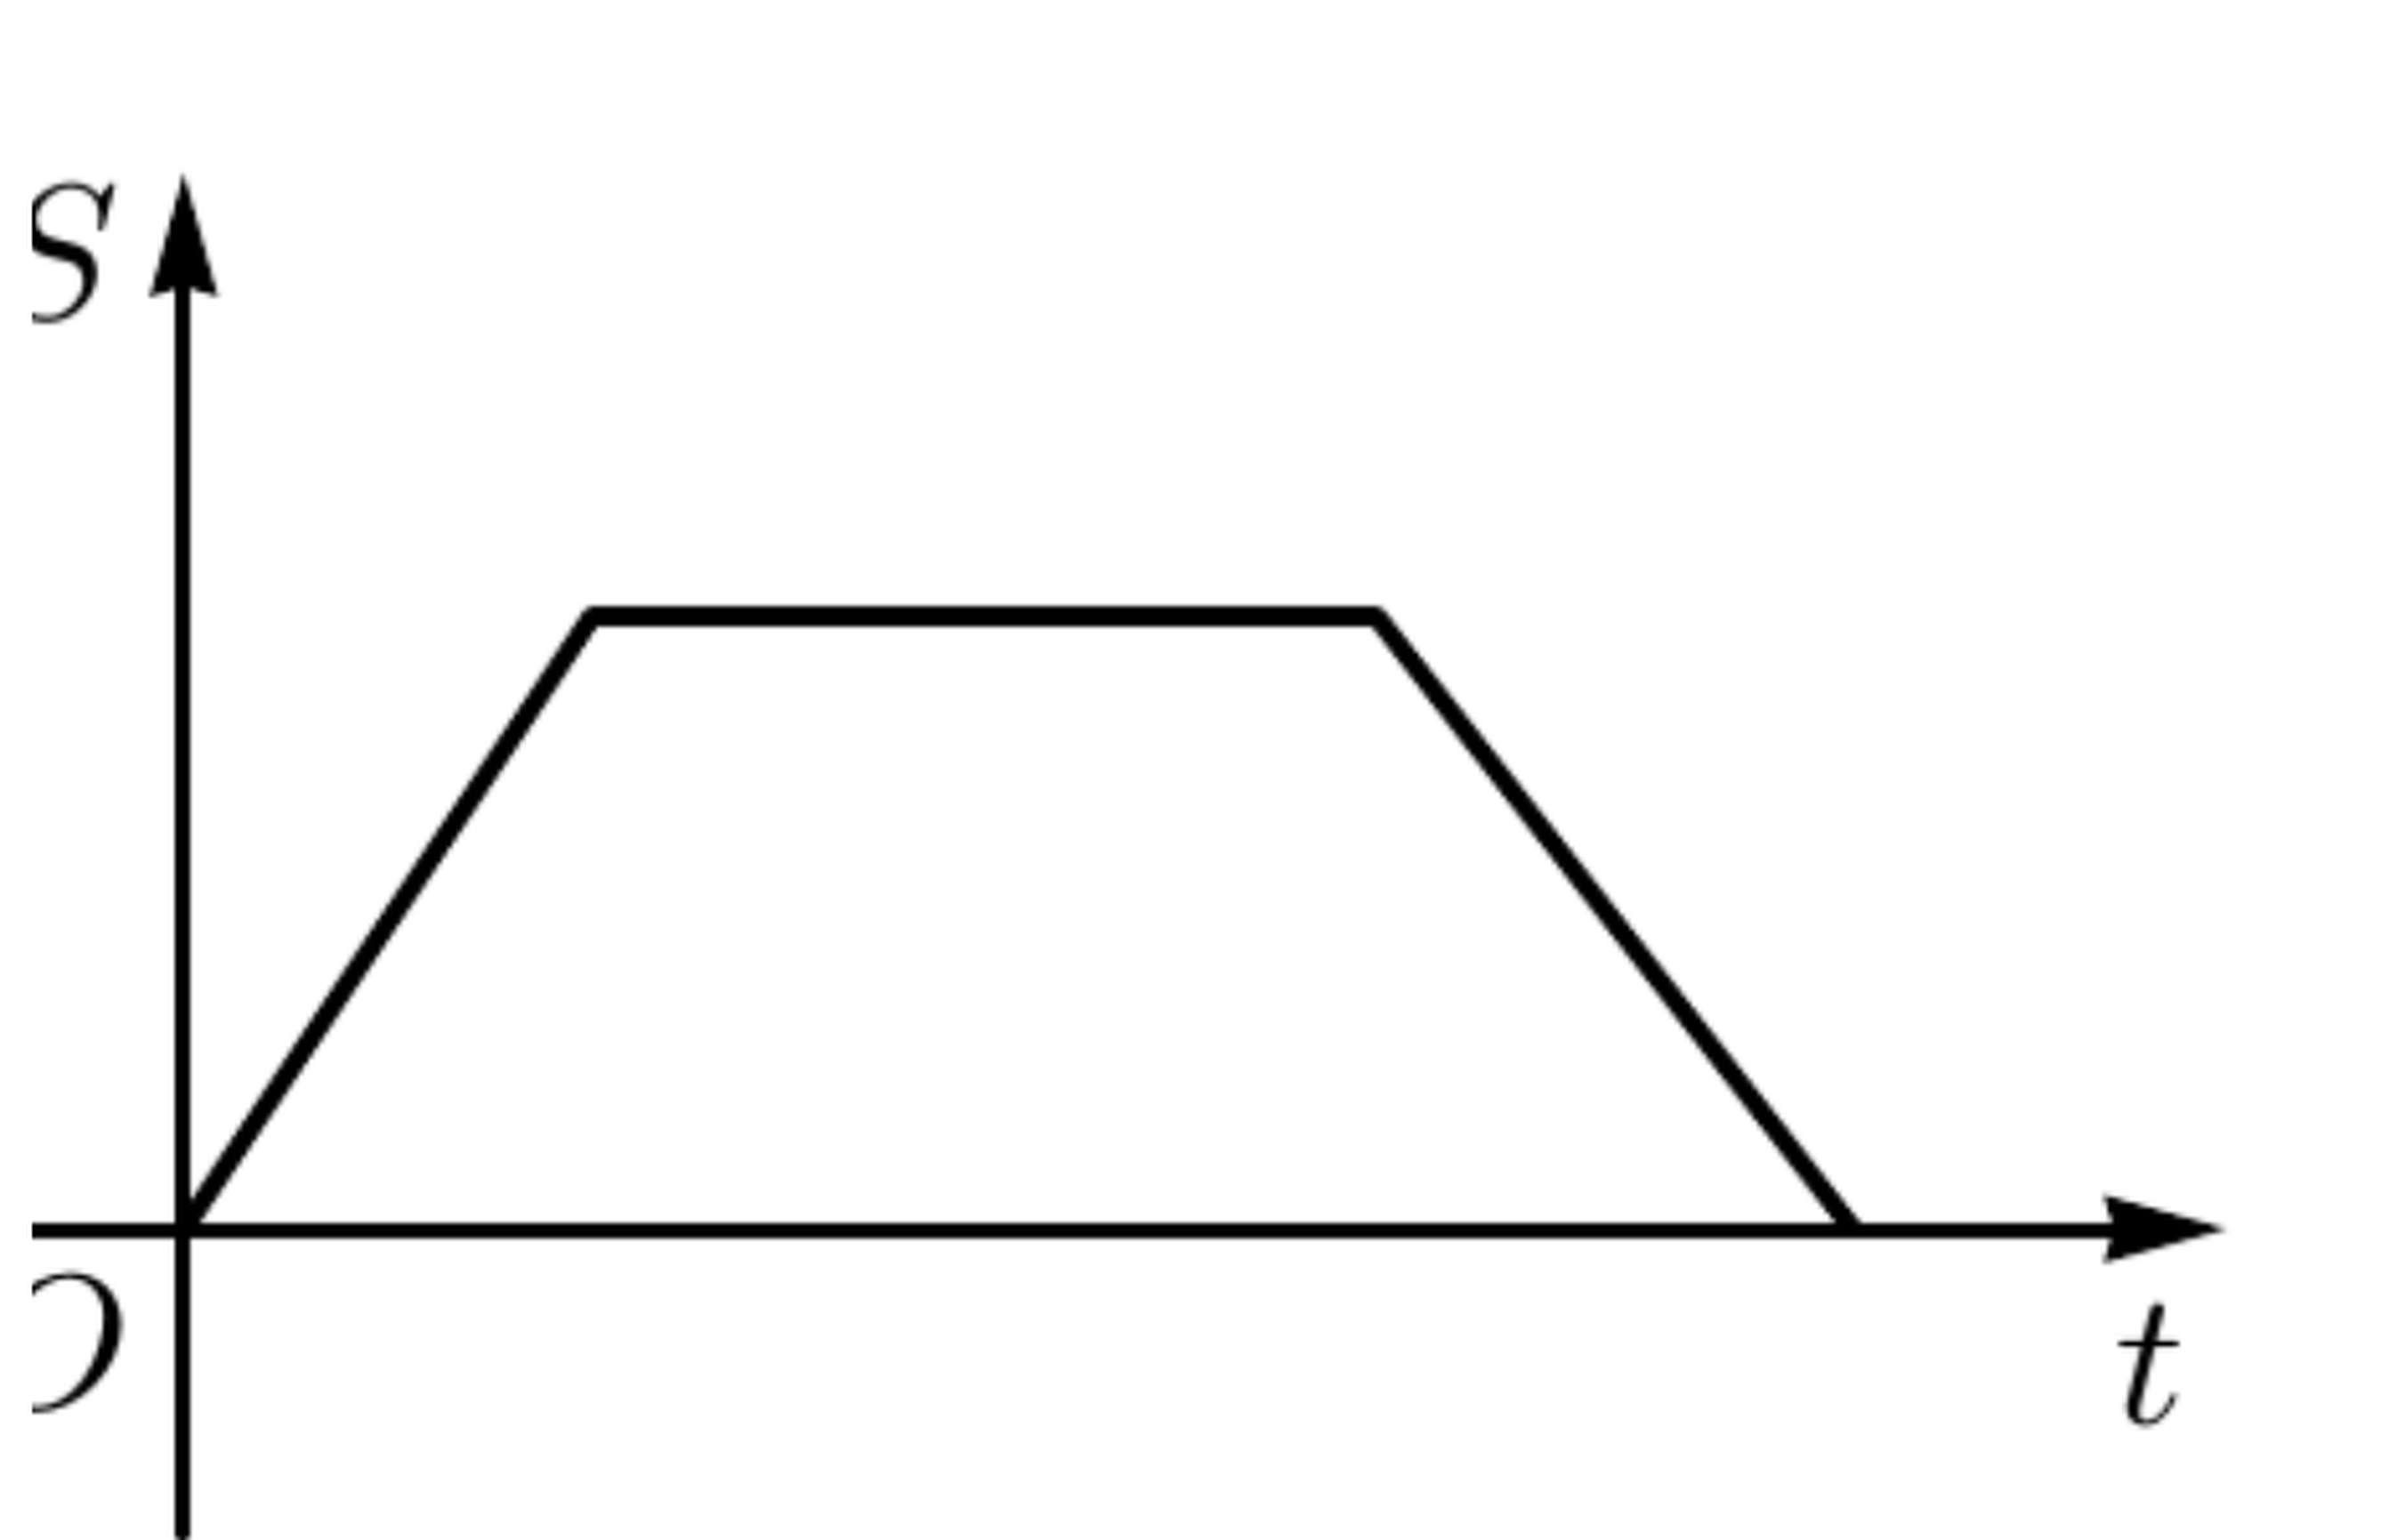
\includegraphics[width=0.34\textwidth]{figures/gao156_q14_st.png}
\end{center}

\keepwithprev
\begin{center}
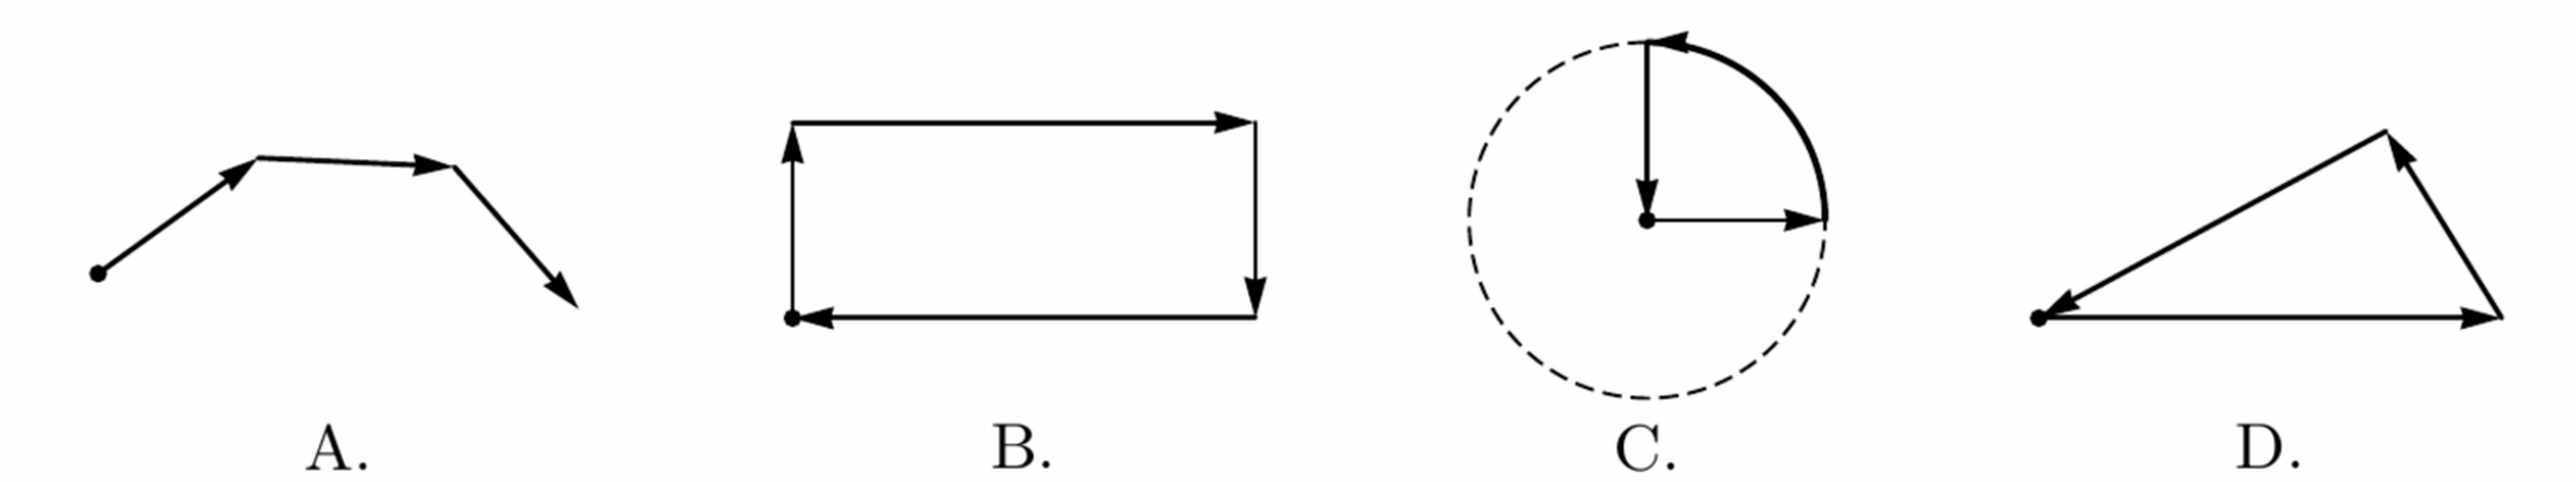
\includegraphics[width=0.86\textwidth]{figures/gao156_q14_opts.png}
\end{center}

\ifanswer
\solbegin
\step{由王老师锻炼时所走的离家距离（$S$）与行走时间（$t$）之间的函数关系图，}
\step{得在中间一段时间里，他到家的距离为定值，}
\step{故他所走的路程是一段以家为圆心的圆弧，故选 $C$.}
\solend
\fi

% === Q15 === 解析内曲线交点图（仅答案版出）；解析 4 行，故选 B
\item 已知 $a+2^a=b+\log_2 b=c+\log_3 c=k$，若 $k<1$，则\mbox{（\quad）}

\keepwithprev
A. $c<a<b$\qquad B. $a<c<b$\qquad C. $b<a<c$\qquad D. $a<b<c$

\ifanswer
\solbegin
\step{因为 $a+2^a=b+\log_2 b=c+\log_3 c=k$，}
\step{所以 $2^a=-a+k$，$\log_2 b=-b+k$，$\log_3 c=-c+k$，其中 $k<1$；}
\step{分别作出 $y=2^x$，$y=\log_2 x$，$y=\log_3 x$ 和 $y=-x+k$ 的图象，}

\begin{center}
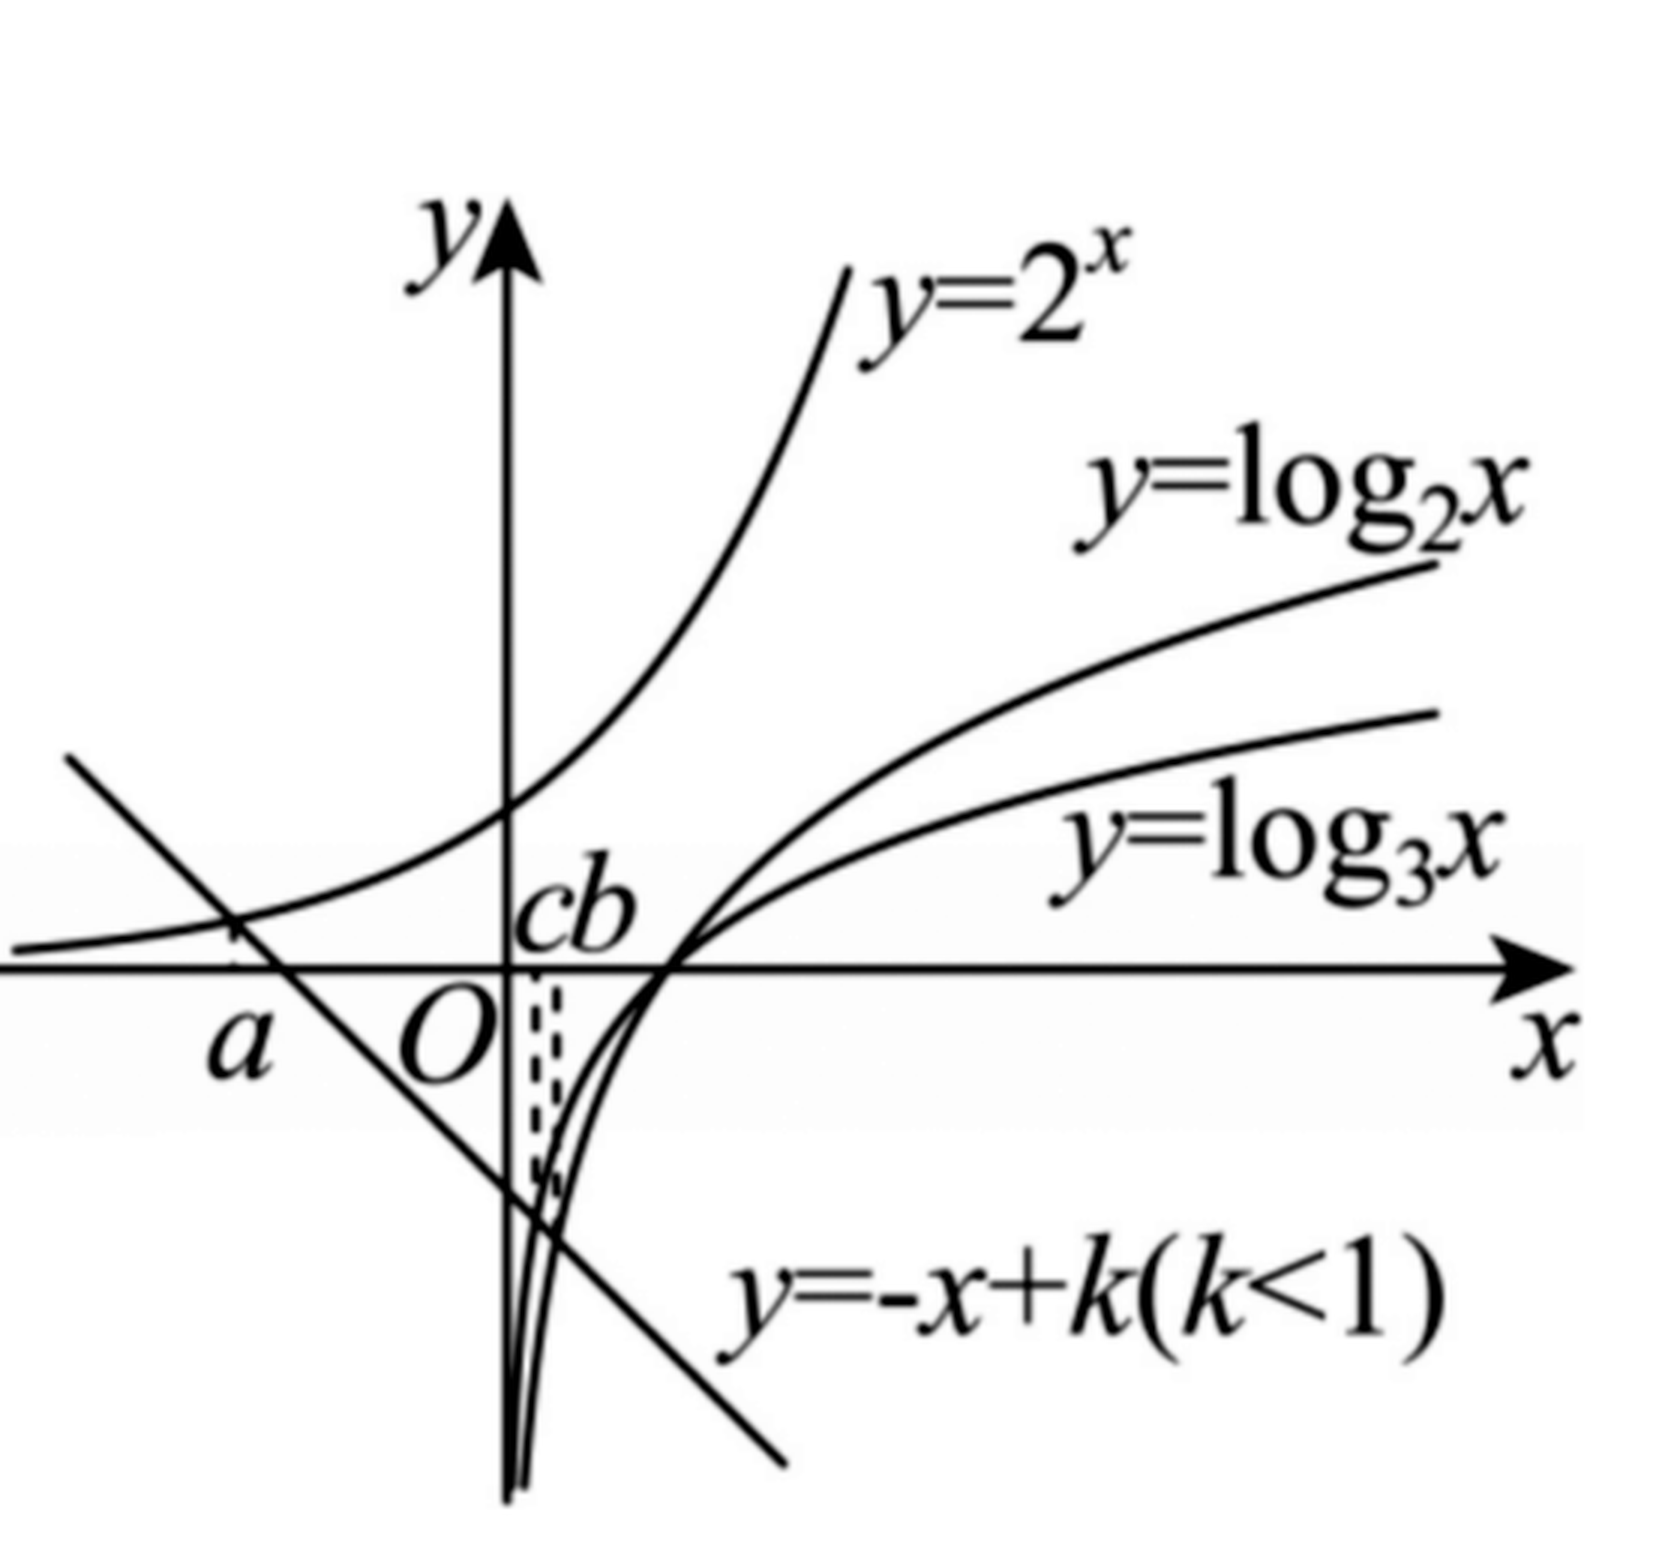
\includegraphics[width=0.52\textwidth]{figures/gao156_q15_curves.png}
\end{center}

\step{如图所示，由图象得 $a<c<b$. 故选 $B$.}
\solend
\fi

% === Q16 === ①② 文本圈数字、"一阶/二阶不动点""稳定点"自定义名词；解析 5 行，故选 A
\item 对定义域为 $I$ 的函数 $y=f(x)$，若存在 $x_0\in I$ 使得 $f(x_0)=x_0$，则称 $x_0$ 是函数 $f(x)$ 的
一阶不动点，简称不动点；若存在 $x_0\in I$ 使得 $f(f(x_0))=x_0$，则称 $x_0$ 是函数 $f(x)$ 的二阶
不动点，简称稳定点. 现有如下两个命题：①存在函数非 $y=x$ 且有无穷多个不动点；②
存在函数有无穷多个稳定点，且这些稳定点不都是不动点. 则\mbox{（\quad）}

\keepwithprev
A. ①成立，②成立\qquad\qquad B. ①成立，②不成立

C. ①不成立，②成立\qquad\qquad D. ①不成立，②不成立

\ifanswer
\solbegin
\step{①取定义在全体实数上的 $f(x)=\lvert x\rvert$，其不动点为一切非负实数，有无穷多个，}
\step{且 $f(-1)=1\ne-1$，①成立.}
\step{②取定义在全体实数上的 $g(x)=-x$，则 $g(g(x))=-(-x)=x$，}
\step{全体实数都是稳定点，而不动点只有 0，②成立.}
\step{故选 $A$.}
\solend
\fi

\end{enumerate}

\bigsec{三、解答题}

\begin{enumerate}
\setcounter{enumi}{16}

% === Q17 === $A\cap B$、$B\cap C$、\varnothing、\mid；解析 6 行
\item 设集合 $A=\{x\mid-1\leqslant x\leqslant2\}$，$B=\{x\mid2m<x<1\}$，$C=\{x\mid x<-1$ 或 $x>2\}$.

(1) 若 $A\cap B=B$，求实数 $m$ 的取值范围；

(2) 若 $B\cap C$ 中只有一个整数，求实数 $m$ 的取值范围.

\ifanswer
\solbegin
\step{(1) 当 $m\geqslant\dfrac12$ 时，$B=\varnothing$，满足 $A\cap B=B$.}
\step{当 $m<\dfrac12$ 时，$A\cap B=B$ 等价于 $2m\geqslant-1$，得 $-\dfrac12\leqslant m<\dfrac12$.}
\step{因此 $m$ 的取值范围为 $\left[-\dfrac12,+\infty\right)$.}
\step{(2) $B\cap C=\{x\mid2m<x<-1\}$，其中只有一个整数时，该整数必为 $-2$.}
\step{包含 $-2$ 且不包含 $-3$，等价于 $-3\leqslant2m<-2$，}
\step{因此 $m$ 的取值范围为 $\left[-\dfrac32,-1\right)$.}
\solend
\fi

% === Q18 === 幂函数 $x^{-\frac13}$、$m\in\R$；解析 12 行，跨 05—06 页
\item 已知幂函数 $f(x)=(3m^2-2m)x^m$（$m\in\R$）在定义域上不单调.

(1) 求函数 $f(x)$ 的解析式；

(2) 若 $f(a+1)<f(-2a+3)$，求实数 $a$ 的取值范围.

\ifanswer
\solbegin
\step{(1) 由幂函数的定义，$3m^2-2m=1$，即 $(3m+1)(m-1)=0$，得 $m=1$ 或 $m=-\dfrac13$.}
\step{当 $m=1$ 时，$f(x)=x$ 在定义域上单调递增，不合题意.}
\step{当 $m=-\dfrac13$ 时，$f(-1)=-1<f(1)=1$，而 $f(1)=1>f(8)=\dfrac12$，}
\step{故 $f(x)$ 在定义域上不单调.}
\step{因此 $f(x)=x^{-\frac13}$，定义域为 $(-\infty,0)\cup(0,+\infty)$.}
\step{(2) 有意义的条件为 $a\ne-1$ 且 $a\ne\dfrac32$.}
\step{当 $a<-1$ 时，$a+1<0<-2a+3$，有 $f(a+1)<0<f(-2a+3)$，}
\step{不等式成立.}
\step{当 $-1<a<\dfrac32$ 时，利用 $f(x)$ 在 $(0,+\infty)$ 上单调递减，}
\step{原不等式等价于 $a+1>-2a+3$，得 $\dfrac23<a<\dfrac32$.}
\step{当 $a>\dfrac32$ 时，$f(a+1)>0>f(-2a+3)$，不等式不成立.}
\step{所以 $a\in(-\infty,-1)\cup\left(\dfrac23,\dfrac32\right)$.}
\solend
\fi

% === Q19 === 两套解法（法一红字 \stepm，法二无标签）；\Delta 与 \subseteq；解析 21 行，跨 06—08 页
\item 已知 $a,c\in\R$，函数 $f(x)=\dfrac{x^2+(3a+1)x+c}{x+a}$.

(1) 若 $a=0$，求函数的定义域，并判断是否存在 $c$ 使得 $y=f(x)$ 图像关于原点对称，说明理由；

(2) 若函数过点 $(1,3)$，且函数 $y=f(x)$ 与 $x$ 轴负半轴有两个不同交点，求此时 $c$ 的值和 $a$ 的取值范围.

\ifanswer
\solbegin
\step{(1) 当 $a=0$ 时，$f(x)=\dfrac{x^2+(3a+1)x+c}{x+a}=\dfrac{x^2+x+c}{x}=x+\dfrac cx+1$，}
\step{故定义域为 $(-\infty,0)\cup(0,+\infty)$；}
\step{若存在实数 $c$，使得函数 $f(x)$ 为奇函数，则必有 $f(x)+f(-x)=0$，}
\step{而 $x+\dfrac cx+1+(-x)+\dfrac c{-x}+1=2\ne0$，}
\step{所以不存在实数 $c$，使得函数 $f(x)$ 为奇函数；}
\step{(2) 函数 $f(x)$ 的图像过点 $(1,3)$，则 $f(1)=\dfrac{1+(3a+1)+c}{1+a}=\dfrac{3a+c+2}{a+1}=3$，}
\step{解得 $c=1$，所以 $f(x)=\dfrac{x^2+(3a+1)x+1}{x+a}$，}
\stepm{法一：}{令 $f(x)=0$，则 $x^2+(3a+1)x+1=0$，此时方程有两不等负根，}
\step{则有 $\begin{cases}\Delta=(3a+1)^2-4>0\\-(3a+1)<0\end{cases}\Rightarrow\begin{cases}a>\dfrac13\text{ 或 }a<-1\\a>-\dfrac13\end{cases}\Rightarrow a>\dfrac13$，}
\step{注意到分母 $x+a\ne0$，则 $x\ne-a$，}
\step{若 $x=-a$ 也是方程 $x^2+(3a+1)x+1=0$ 的解，}
\step{代入方程 $(-a)^2+(3a+1)(-a)+1=0\Rightarrow2a^2+a-1=(a+1)(2a-1)=0$，}
\step{解得 $a=-1$ 或 $a=\dfrac12$，从而 $a\ne\dfrac12$，}
\step{综上，实数 $a$ 的取值范围为 $\left(\dfrac13,\dfrac12\right)\cup\left(\dfrac12,+\infty\right)$.}
\step{令 $g(x)=x^2+(3a+1)x+1$，与 $x$ 轴负半轴有两个交点，}
\step{则 $\begin{cases}-(3a+1)<0\\\Delta=(3a+1)^2-4>0\end{cases}\Rightarrow a>\dfrac13$.}
\step{注意到分母 $x+a\ne0$，则 $x\ne-a$，}
\step{若 $x=-a$ 也是方程 $x^2+(3a+1)x+1=0$ 的解，}
\step{代入方程 $(-a)^2+(3a+1)(-a)+1=0\Rightarrow2a^2+a-1=(a+1)(2a-1)=0$，}
\step{解得 $a=-1$ 或 $a=\dfrac12$，从而 $a\ne\dfrac12$，}
\step{综上，实数 $a$ 的取值范围为 $\left(\dfrac13,\dfrac12\right)\cup\left(\dfrac12,+\infty\right)$.}
\solend
\fi

% === Q20 === $Q$ 常数段 80000 照录；cases 与基本不等式；解析 10 行，跨 08—09 页
\item 某工厂生产某种零件的固定成本为 20000 元，每生产一个零件要增加投入 100 元，已知
总收入 $Q$（单位：元）关于产量 $x$（单位：个）满足函数：$Q=\begin{cases}400x-\dfrac12x^2,&0\leqslant x\leqslant400\\80000,&x>400\end{cases}$.

(1) 将利润 $P$（单位：元）表示为产量 $x$ 的函数；（总收入$=$总成本$+$利润）

(2) 当产量为何值时，零件的单位利润最大？最大单位利润是多少元？（单位利润$=$利润$\div$产量）

\ifanswer
\solbegin
\step{(1) 当 $0\leqslant x\leqslant400$ 时，}
\step{$P(x)=400x-\dfrac12x^2-20000-100x=-\dfrac12x^2+300x-20000$，}
\step{当 $x>400$ 时，$P(x)=80000-100x-20000=60000-100x$，}
\step{故 $P(x)=\begin{cases}-\dfrac12x^2+300x-20000,&0\leqslant x\leqslant400\\60000-100x,&x>400\end{cases}$.}
\step{(2) 设零件的单位利润为 $g(x)$，则 $g(x)=\begin{cases}-\dfrac12x-\dfrac{20000}{x}+300,&0\leqslant x\leqslant400\\\dfrac{60000}{x}-100,&x>400\end{cases}$，}
\step{当 $0\leqslant x\leqslant400$ 时，}
\step{$g(x)=300-\left(\dfrac12x+\dfrac{20000}{x}\right)\leqslant300-2\sqrt{\dfrac x2\cdot\dfrac{20000}{x}}=100$，}
\step{当且仅当 $\dfrac x2=\dfrac{20000}{x}$，即 $x=200$ 时取等号，}
\step{当 $x>400$ 时，$g(x)=\dfrac{60000}{x}-100$，此时无最值，}
\step{故当产量为 200 个，零件的单位利润最大，最大单位利润是 100 元.}
\solend
\fi

% === Q21 === 上升集定义、$D(x_0)=\{d\in\R\mid\cdots\}$、①②③ 文本圈数字、
%            \subseteq 带下划线、$-2^{-x}$；解析 19 行，跨 09—10 页
\item 已知函数 $y=f(x)$ 的定义域为 $\R$. 对任意 $x_0\in\R$，定义集合
$D(x_0)=\{d\in\R\mid f(x_0+d)>f(x_0)\}$，则称 $D(x_0)$ 为函数 $y=f(x)$ 在 $x_0$ 处的上升集.

(1) 若 $f(x)=1-x$，求 $D(-1)$；

(2) 若 $f(x)=\begin{cases}2^x,&x<0\\0,&x=0\\-2^{-x},&x>0\end{cases}$，求 $D(x)$；

(3) 设 $y=f(x)$ 满足：①当 $x<0$ 时，$f(x)=2^x$；②若 $f(x_1)\leqslant f(x_2)$，则
$D(x_2)\subseteq D(x_1)$；③当 $0<x<1$ 时，$f(x)<f(0)$. 证明：$f(0)\geqslant1$.

\ifanswer
\solbegin
\step{(1) $f(-1+d)>f(-1)\Leftrightarrow2-d>2\Leftrightarrow d<0$，所以 $D(-1)=(-\infty,0)$.}
\step{(2) 函数在 $(-\infty,0)$、$(0,+\infty)$ 上分别严格递增，}
\step{且这两个区间上的函数值分别为正、负，$f(0)=0$.}
\step{当 $x<0$ 时，$f(x+d)>f(x)\Leftrightarrow x<x+d<0\Leftrightarrow0<d<-x$，}
\step{当 $x=0$ 时，$f(d)>f(0)\Leftrightarrow d<0$，}
\step{当 $x>0$ 时，$f(x+d)>f(x)\Leftrightarrow x+d\leqslant0$ 或 $x+d>x$}
\step{$\Leftrightarrow d\leqslant-x$ 或 $d>0$，}
\step{因此 $D(x)=\begin{cases}(0,-x),&x<0\\(-\infty,0),&x=0\\(-\infty,-x]\cup(0,+\infty),&x>0\end{cases}$.}
\step{(3) 任取 $a\in(-1,0)$，}
\step{令 $d=-\dfrac a2$，则 $0<d<1$，且 $f(a+d)=2^{\frac a2}>2^a=f(a)$，}
\step{所以 $d\in D(a)$；}
\step{由③，$f(d)<f(0)$，所以 $d\notin D(0)$.}
\step{若 $f(0)\leqslant f(a)$，由②得 $D(a)\subseteq D(0)$，与上述结论矛盾.}
\step{因此，对任意 $a\in(-1,0)$，都有 $f(0)>2^a$.}
\step{特别地 $f(0)>2^{-\frac12}>0$.}
\step{若 $f(0)<1$，取 $a=\dfrac12\log_2 f(0)$，则 $-\dfrac14<a<0$，且}
\step{$2^a=\sqrt{f(0)}>f(0)$，}
\step{与 $f(0)>2^a$ 矛盾.}
\step{所以 $f(0)\geqslant1$.}
\solend
\fi

\end{enumerate}

\end{document}
"
% 紧凑版：xelatex "\def\iscompact{1}% 高一156_大同中学_期中.tex
%   —— 高一上数学"2026-2027 年大同中学高一上期中"（试卷版/答案版/紧凑版）
% 试卷版：xelatex 高一156_大同中学_期中.tex
% 答案版：xelatex "\def\isanswer{1}\input{高一156_大同中学_期中.tex}"
% 紧凑版：xelatex "\def\iscompact{1}\input{高一156_大同中学_期中.tex}"
%
% ① 原始材料：微信公众号"魔都数学加油站"文章，连载"27学年高一156"，原文标题
% "27学年高一156——2026-2027年上海市大同中学高一上期中"；
% 原文链接：https://mp.weixin.qq.com/s/xLtS5tyjCPJIWCIBohwGvw 。
% 正文为 10 张 PNG 页（01/02/03/04/05/06/07/08/09/10 各页分辨率混排
% 2560×3620 与 4762×6735，逐页按各自分辨率裁图核对）。
% 体例：讲评版——填空 3—12（10 题）、选择 13—16（4 题）、解答 17—21（5 题），
% 共 19 题，自第 3 题起编（1、2 未印在本篇）；Q3 只印【答案】、其余 18 题
% 逐题印【解析】（逐题核实，见 ②）。题目、答案、解析均据原图转录；卷面粉红色
% 水印"魔都数学加油站"及公众号页脚未录入。
%
% 卷首标题：原卷印作"2026-2027 年大同中学高一上期中"，年份区间按全稿惯例排 en dash；
% 原卷卷面未印副标题，本稿按同期中卷知识模块口径补出"集合与常用逻辑用语、不等式、函数"。
%
% ② 与原卷的排版差异：
%   ① 原文从第 3 题起，本稿保留原题号；共 19 题三节，解答题 5 题到 21；
%   ② 混合体例：第 3 题只印【答案】、无【解析】，按 高一140 第 5 题／高一145
%      第 3 题／高一151 第 7 题成例另提 \ans{}、不补造解析；其余 18 题印
%      【解析】、用 \solbegin…\solend；四道选择题答案在解析末句"故选 C／C／B／A"
%      （逐个放大复核）、括号 \mbox{（\quad）} 留空、不另提 \ans{}；答案版
%      【答案】/【解析】标记数 = 19 = 全卷题数（1 个 \ans ＋ 18 个 \solbegin）；
%   ③ 原卷卷面未印副标题，本稿按知识模块口径补出；
%   ④ 原卷填空横线按全稿惯例排 \blankline[4.4em]；选择题括号排 \mbox{（\quad）}、
%      选项段前按惯例各加 \keepwithprev；解答题不留作答区、不加 \anspace
%      （原卷为讲评版，109—113 起全稿不用 \anspace）；
%   ⑤ 数集：Q3"$x\in\R$"、Q18"$m\in\R$"、Q19"$a,c\in\R$"、Q21"定义域为 \R"
%      "任意 $x_0\in\R$""$d\in\R$"原卷印正体粗体 R，按全稿惯例归一 \R；
%      绝对值排 \lvert…\rvert（Q11 $\lvert2^x-1\rvert$、Q16 $\lvert x\rvert$），
%      集合描述竖线排 \mid（Q17 $A=\{x\mid\cdots\}$、Q21 $D(x_0)=\{d\in\R\mid\cdots\}$），
%      空集 \varnothing（Q17"$B=\varnothing$"），不等号按全稿惯例排 \leqslant／\geqslant；
%   ⑥ 子集符号逐处照录不统一：Q21 (3) 题干"$D(x_2)\subseteq D(x_1)$"与解析
%      "$D(a)\subseteq D(0)$"均印带下划线 ⊆，照录 \subseteq；本卷无单线 ⊂ 用例；
%   ⑦ 判别式：Q19 两套解法"$\Delta=(3a+1)^2-4>0$"印等腰偏高 \Delta，照录 \Delta；
%      本卷无扁三角 \triangle 用例；
%   ⑧ 红字照录为黑体：Q19 (2) 解析第一套解法行首"法一："原卷排**红色加粗**，
%      按 高一53 成例排 \stepm{法一：}{…}（加粗着色、不改黑色基调），全库无红字
%      排字先例、本稿不引入红色定义，文件头注明；第二套解法原卷直接以
%      "令 $g(x)=x^2+(3a+1)x+1$，与 $x$ 轴负半轴有两个交点，"另起，
%      **未印"法二："标签**（逐页像素级复核：07 页仅 1437—1475 一处红字，
%      08 页无红字），照录为普通 \step、不补造标签；
%   ⑨ 文本模式圈数字逐处照录：Q12 解析 ①② 两情形、Q16 两则命题与四个选项及
%      解析的 ①②、Q21 (3) 三条件 ①②③ 与解析"由③""由②"，均为印刷圈数字
%      （非 \textcircled、非数学模式），计入圈数字实测；
%   ⑩ 自定义名词照录：Q16"一阶不动点，简称不动点""二阶不动点，简称稳定点"、
%      Q21"上升集"；Q16 题干"存在函数非 $y=x$ 且有无穷多个不动点"照录；
%   ⑪ 中文弯引号照录：Q3""存在 $x\in\R$，$x^3-1\leqslant0$" 否定形式为"、
%      Q13"使"$\dfrac{x+1}{1-x}\geqslant0$"成立的必要不充分条件是"；
%      注释里一律 ASCII 引号；数学式内 CJK 用 \text{}（Q19 cases 内"或"）；
%   ⑫ 半角逗号在数学组之间是全稿惯例、非笔误，逐处照录（$a,c$、$x,y$、$a,b$
%      之类）；行末西文句点 ASCII `.`；行中全角逗号／顿号照录；
%   ⑬ 复杂式照录别简化：Q6 $\left(\dfrac{1}{\sqrt a}\right)^{\frac27}\cdot\sqrt[7]{a^3}$
%      与解析 $a^{\frac{12}{7}-\frac17+\frac37}$、Q8 $2\sqrt4+5=9$（$\sqrt4$ 未化简）、
%      Q9 $\left(\sqrt x+\dfrac{1}{\sqrt x}\right)^3$、Q12 $\dfrac{4a-(2-a)^2}{4a}$、
%      Q18 $f(8)=\dfrac12$、Q19 $2a^2+a-1=(a+1)(2a-1)=0$、Q20 $Q$ 的常数段
%      $80000$（不是 $80000-100x$）与 $2\sqrt{\dfrac x2\cdot\dfrac{20000}{x}}$、
%      Q21 $f(a+d)=2^{\frac a2}>2^a=f(a)$ 与 $2^a=\sqrt{f(0)}>f(0)$ 等；
%      \left…\right 不得拆到不同 $…$ 组（Q5 $\left(0,\dfrac12\right)$、
%      Q12 $\left[0,4+2\sqrt3\right)$、Q17 $\left[-\dfrac12,+\infty\right)$、
%      Q19 $\left(\dfrac13,\dfrac12\right)\cup\left(\dfrac12,+\infty\right)$、
%      Q20 $\left(\dfrac12x+\dfrac{20000}{x}\right)$ 等）；cases 块整体算一个印刷行；
%   ⑭ 一条 \step = 原卷解析的一个印刷行；别并折行、别拆行。跨页续印按题合并
%      （Q6 的 01 页上下题干重复印、Q8 的 01—02 页、Q12 的 02—03 页、
%      Q15 的 04 页上下、Q16 的 04—05 页、Q17 的 05 页上下、Q18 的 05—06 页、
%      Q19 的 06—08 页、Q20 的 08—09 页、Q21 的 09—10 页）；
%      跨半页重叠行（Q12 的"②若 …"、Q18 的"原不等式等价于 …"、
%      Q20 的"【解析】(1) 当 $0\leqslant x\leqslant400$ 时，"、Q21 的
%      "【解析】(1) $f(-1+d)>f(-1)\cdots$"与"与 $f(0)>2^a$ 矛盾."）
%      只算一个印刷行；
%   ⑮ 配图：全卷 3 组（逐页通读 10 页确认）——
%      · Q14 题干 S-t 梯形图（03 页右下，离家距离 S 对行走时间 t），题目配图、
%        三版都出，裁 figures/gao156_q14_st.png；
%      · Q14 四幅路线选项（04 页上部，A/B/C/D 四幅横排、C 为以家为圆心的圆弧），
%        题目配图、三版都出，合并成一张，裁 figures/gao156_q14_opts.png；
%      · Q15 解析内曲线交点图（04 页右下，$y=2^x$、$y=\log_2x$、$y=\log_3x$
%        与 $y=-x+k$），仅答案版出，裁 figures/gao156_q15_curves.png；
%      3 图均取自原卷截图，去粉色水印、去色、3×~4× LANCZOS 放大；
%      Q14 题干"题干＋两图"整块用 \needvspace 守卫推走（守卫放 \item 之前，
%      见 高一154 Q15／高一136 Q13 成例）；Q15 解析内图放 \ifanswer 内
%      \solbegin…\solend 的两 \step 之间（高一108 第 6 题／高一154 附加题 2 成例）；
%      其余各页逐页确认无其它题目配图、无解析配图、无表格；10 页下半仅水印、无正文。
%
% ③ 行数复核：一条 \step = 原卷解析的一个印刷行，cases 块作一个印刷行计。
%   逐题数（主会话逐页核对定稿）：Q3：0（只印【答案】、提 \ans{}，不计入 \step 账）；
%   Q4：1；Q5：1；Q6：1；Q7：1；Q8：3；Q9：2；Q10：2；Q11：5；Q12：12；
%   Q13：3；Q14：3；Q15：4；Q16：5；Q17：6；Q18：12；Q19：21；Q20：10；Q21：19。
%   合计 111 行（110 条 \step ＋ 1 条 \stepm），与原卷逐题印刷行相等。
%   全卷 19 题：Q3 一处 \ans{} ＋ 其余 18 题设 \solbegin…\solend，
%   答案版【答案】/【解析】标记数 = 19 = 全卷题数。
%
% ④ 页码分布（供回原图复核）：
%   卷首标题＋"一、填空题"＋Q3 题干＋【答案】、Q4 题干＋解析 1 行、
%   Q5 题干＋解析 1 行、Q6 题干首行在 01 页上半；
%   Q6 题干（重复印）＋解析 1 行、Q7 题干＋解析 1 行、Q8 题干＋解析前 2 行
%   在 01 页下半；Q8 解析末行、Q9 题干＋解析 2 行、Q10 题干＋解析 2 行、
%   Q11 题干首行在 02 页上半；Q11 题干（重复印）＋解析 5 行、
%   Q12 题干＋解析首行在 02 页下半；Q12 解析中 9 行在 03 页上半；
%   Q12 解析末 2 行＋"二、选择题"标题＋Q13 题干＋选项＋解析 3 行＋
%   Q14 题干首行在 03 页下半；Q14 题干续行＋四幅选项图＋解析 3 行＋
%   Q15 题干＋选项＋解析前 2 行＋Q16 题干在 04 页上半；
%   Q15 解析后 2 行＋曲线图＋Q16 选项＋解析前 2 行在 04 页下半；
%   Q16 解析后 3 行＋"三、解答题"标题＋Q17 题干＋两问＋解析 (1) 3 行
%   在 05 页上半；Q17 解析 (2) 3 行＋Q18 题干＋两问＋解析 (1) 首 2 行
%   在 05 页下半；Q18 解析 (1)(2) 中 8 行在 06 页上半；Q18 解析末 2 行＋
%   Q19 题干＋两问＋解析 (1) 首行在 06 页下半；Q19 解析 (1) 后 4 行＋
%   (2) 前 2 行＋法一 2 行在 07 页上半；法一后 5 行＋法二前 3 行在 07 页下半；
%   法二后 4 行＋Q20 题干＋两问＋解析 (1) 首行在 08 页上半；
%   Q20 解析 (1) 后 3 行＋(2) 前 5 行在 08 页下半；Q20 解析 (2) 末 2 行＋
%   Q21 题干＋三问＋解析 (1) 首行在 09 页上半；Q21 解析 (1)（重复印）＋
%   (2) 8 行＋(3) 首行在 09 页下半；Q21 (3) 解析中 8 行在 10 页上半；
%   Q21 (3) 末 2 行在 10 页下半。本稿按题连排，不丢行、不并折行；
%   全卷末题为第 21 题，无附加题节。
%
\documentclass[a4paper,11pt]{article}
\usepackage{common}

\begin{document}

\examtitlest[3]{2026--2027 年大同中学高一上期中}{集合与常用逻辑用语、不等式、函数}

\bigsec{一、填空题}

\begin{enumerate}
\setcounter{enumi}{2}

% === Q3 === 只印【答案】、无【解析】；R 正体粗体 \R；中文弯引号照录
\item “存在 $x\in\R$，$x^3-1\leqslant0$” 否定形式为\blankline[4.4em].

\ifanswer
\ans{对任意 $x\in\R$，$x^3-1>0$}
\fi

% === Q4 === 解析 1 行
\item 若实数 $a>0$ 且 $a\ne1$，函数 $y=a^{x-3}+1$ 的图像恒过定点 $P$，则点 $P$ 的坐标为\blankline[4.4em].

\ifanswer
\solbegin
\step{当 $x=3$ 时，$y=a^0+1=2$，与 $a$ 无关，所以定点为 $P(3,2)$.}
\solend
\fi

% === Q5 === 解析 1 行
\item 函数 $y=\dfrac{1}{3^x+2}$ 的值域是\blankline[4.4em].

\ifanswer
\solbegin
\step{$3^x\in(0,+\infty)$，因此 $3^x+2\in(2,+\infty)$，值域为 $\left(0,\dfrac12\right)$.}
\solend
\fi

% === Q6 === 根式嵌套照录；解析 1 行；题干跨 01 页上下重复印
\item 已知 $a>0$，化简 $a^{\frac{12}{7}}\cdot\left(\dfrac{1}{\sqrt a}\right)^{\frac27}\cdot\sqrt[7]{a^3}=$\blankline[4.4em].

\ifanswer
\solbegin
\step{原式 $=a^{\frac{12}{7}}\cdot a^{-\frac17}\cdot a^{\frac37}=a^{\frac{12}{7}-\frac17+\frac37}=a^2$.}
\solend
\fi

% === Q7 === 换底公式；解析 1 行
\item 已知 $\log_5 3=a$，用 $a$ 的代数式表示 $\log_{15}125=$\blankline[4.4em].

\ifanswer
\solbegin
\step{$\log_{15}125=\dfrac{\log_5 125}{\log_5 15}=\dfrac{3}{1+\log_5 3}=\dfrac{3}{1+a}$.}
\solend
\fi

% === Q8 === 基本不等式，$\sqrt4$ 照录未化简；解析 3 行，跨 01—02 页
\item 已知 $x>0$，$y>0$，且 $4x+y=xy$，则 $x+y$ 的最小值为\blankline[4.4em].

\ifanswer
\solbegin
\step{由 $4x+y=xy$，得 $\dfrac4y+\dfrac1x=1$，}
\step{则 $x+y=(x+y)\left(\dfrac4y+\dfrac1x\right)=\dfrac{4x}{y}+\dfrac yx+1+4\geqslant2\sqrt4+5=9$，}
\step{当且仅当 $\dfrac{4x}{y}=\dfrac yx$，即 $x=3$，$y=6$ 时取等号，故最小值为 9.}
\solend
\fi

% === Q9 === 解析 2 行
\item 已知 $x^{-1}+x=7$（$x>0$），则 $x^{\frac32}+x^{-\frac32}$ 的值为\blankline[4.4em].

\ifanswer
\solbegin
\step{$x>0$，有 $\sqrt x+\dfrac{1}{\sqrt x}=\sqrt{x+\dfrac1x+2}=3$，}
\step{所以 $x^{\frac32}+x^{-\frac32}=\left(\sqrt x+\dfrac{1}{\sqrt x}\right)^3-3\left(\sqrt x+\dfrac{1}{\sqrt x}\right)=27-9=18$.}
\solend
\fi

% === Q10 === $x_{\min}$；解析 2 行
\item 已知不等式 $x>\dfrac{2a+1}{a-1}$ 对任意的 $x\in[1,2]$ 恒成立，则实数 $a$ 的取值范围是\blankline[4.4em].

\ifanswer
\solbegin
\step{不等式 $x>\dfrac{2a+1}{a-1}$ 对任意的 $x\in[1,2]$ 恒成立，得 $\dfrac{2a+1}{a-1}<x_{\min}=1$，}
\step{即有 $\dfrac{a+2}{a-1}<0$，解得 $-2<a<1$，则实数 $a$ 的取值范围是 $(-2,1)$.}
\solend
\fi

% === Q11 === 分段函数 cases 与绝对值 \lvert…\rvert；解析 5 行
\item 已知函数 $f(x)=\begin{cases}\lvert2^x-1\rvert-a,&x\leqslant2\\\dfrac{3}{x-1}-a,&x>2\end{cases}$，若函数 $y=f(x)$ 图像与 $x$ 轴有三个不同交点，则实数 $a$ 的取值范围是\blankline[4.4em].

\ifanswer
\solbegin
\step{令 $g(x)=f(x)+a$.}
\step{在 $(-\infty,0)$、$[0,2]$、$(2,+\infty)$ 上，$g(x)$ 均严格单调，}
\step{值域依次为 $(0,1)$、$[0,3]$、$(0,3)$.}
\step{每段至多有一个交点，因而恰有三个不同交点，}
\step{当且仅当 $a\in(0,1)\cap[0,3]\cap(0,3)=(0,1)$.}
\solend
\fi

% === Q12 === ①② 文本圈数字、对称轴与最小值式照录；解析 12 行，跨 02—03 页
\item 已知函数 $f(x)=ax^2-(2-a)x+1$，$g(x)=x$，若对于任意实数 $x$，$f(x)$ 与 $g(x)$ 至少有一个为正数，则实数 $a$ 的取值范围是\blankline[4.4em].

\ifanswer
\solbegin
\step{当 $x>0$ 时，$g(x)>0$；当 $x<0$ 时，$g(x)<0$；}
\step{当 $x=0$ 时，$f(0)=1>0$；}
\step{因为对于任意实数 $x$，$f(x)$ 与 $g(x)$ 至少有一个为正数，}
\step{当 $x<0$ 时，因为 $g(x)<0$，所以 $f(x)=ax^2-(2-a)x+1>0$ 恒成立，}
\step{当 $a<0$ 时，显然不成立，}
\step{当 $a=0$ 时，$f(x)=-2x+1>0$，对 $x<0$ 时恒成立，满足题意，}
\step{当 $a>0$ 时，函数图象开口向上，对称轴 $x=\dfrac{2-a}{2a}$，}
\step{①若 $\dfrac{2-a}{2a}\geqslant0$，即 $0<a\leqslant2$ 时，函数 $f(x)$ 在 $(-\infty,0)$ 上严格减，$f(0)=1$，}
\step{故 $f(x)>0$ 对 $x<0$ 时恒成立，满足题意；}
\step{②若 $\dfrac{2-a}{2a}<0$，即 $a>2$ 时，$f(x)_{\min}=f\left(\dfrac{2-a}{2a}\right)=\dfrac{4a-(2-a)^2}{4a}>0$，}
\step{解得 $4-2\sqrt3<a<4+2\sqrt3$，所以 $2<a<4+2\sqrt3$.}
\step{综上，$0\leqslant a<4+2\sqrt3$，故实数 $a$ 的取值范围是 $\left[0,4+2\sqrt3\right)$.}
\solend
\fi

\end{enumerate}

\bigsec{二、选择题}

\begin{enumerate}
\setcounter{enumi}{12}

% === Q13 === 必要不充分条件；cases 块；解析 3 行，故选 C
\item 使 “$\dfrac{x+1}{1-x}\geqslant0$” 成立的必要不充分条件是\mbox{（\quad）}

\keepwithprev
A. $-1\leqslant x<1$\qquad B. $x\leqslant-1$ 或 $x>1$\qquad C. $-1\leqslant x\leqslant1$\qquad D. $x\leqslant-1$ 或 $x\geqslant0$

\ifanswer
\solbegin
\step{由不等式 $\dfrac{x+1}{1-x}\geqslant0$ 得 $\begin{cases}(x+1)(1-x)\geqslant0\\1-x\ne0\end{cases}$，解得 $-1\leqslant x<1$，}
\step{由题意结合选项，$-1\leqslant x<1\Rightarrow-1\leqslant x\leqslant1$ 成立，反之不成立，}
\step{所以 $-1\leqslant x\leqslant1$ 是 $\dfrac{x+1}{1-x}\geqslant0$ 成立的必要不充分条件. 故选 $C$.}
\solend
\fi

% === Q14 === 题干 S-t 图＋四幅路线选项（题目配图，三版都出）；守卫放 \item 之前；解析 3 行，故选 C
\needvspace{9cm}
\item 如图是王老师锻炼时所走的离家距离（$S$）与行走时间（$t$）之间的函数关系图，若
用黑点表示王老师家的位置，则王老师行走的路线可能是\mbox{（\quad）}

\begin{center}
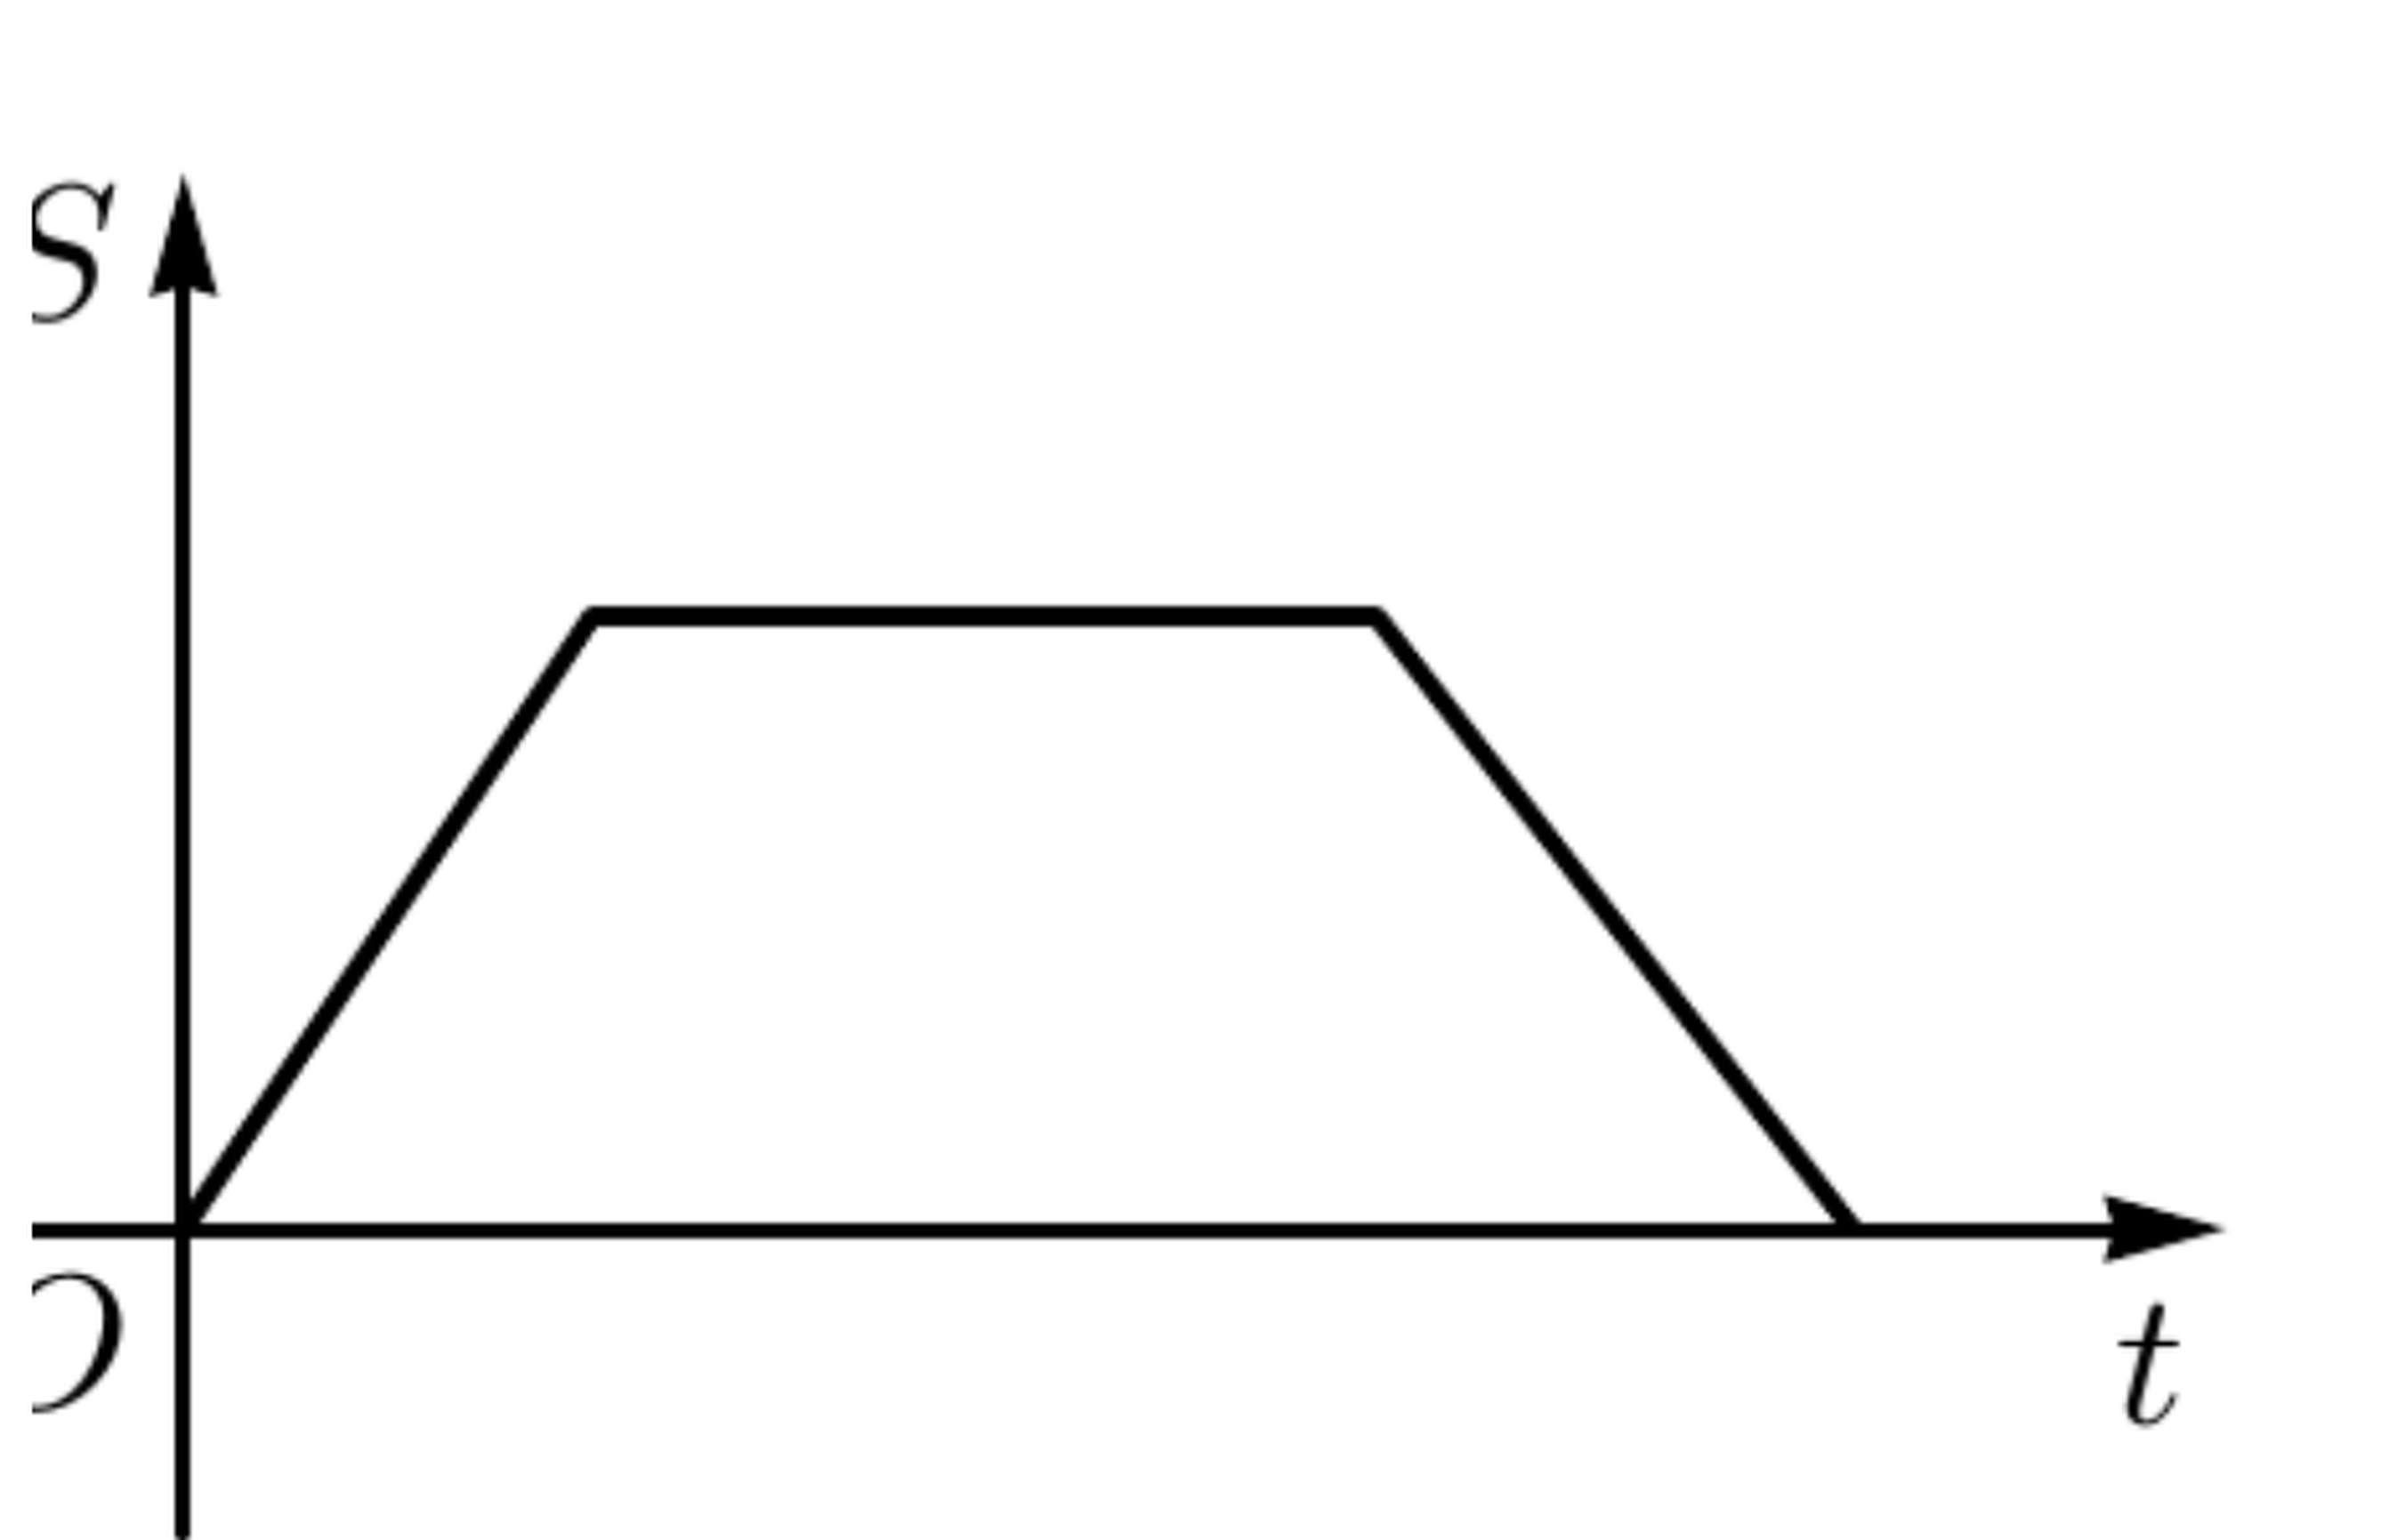
\includegraphics[width=0.34\textwidth]{figures/gao156_q14_st.png}
\end{center}

\keepwithprev
\begin{center}
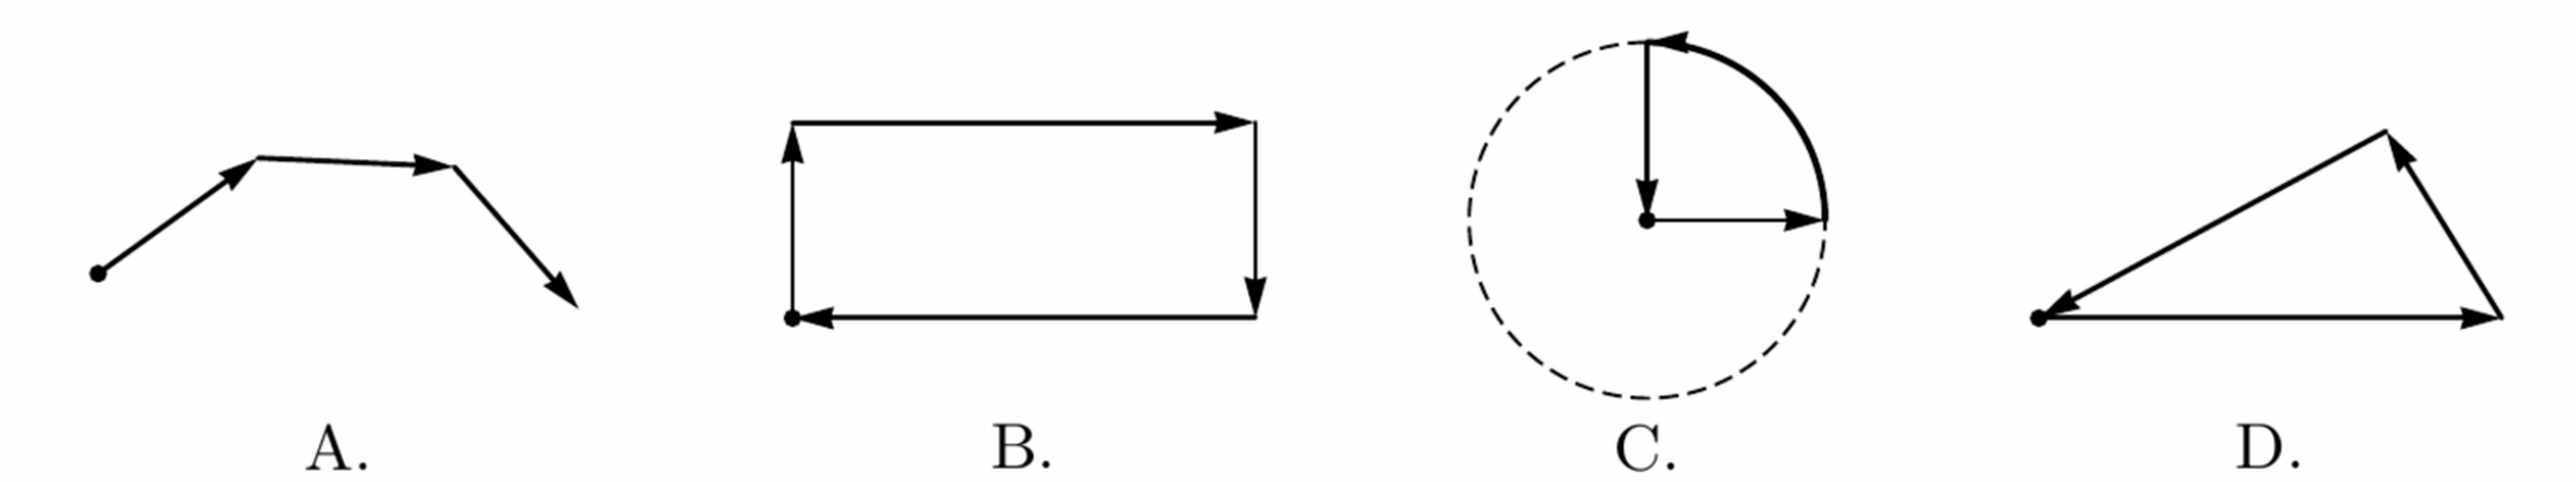
\includegraphics[width=0.86\textwidth]{figures/gao156_q14_opts.png}
\end{center}

\ifanswer
\solbegin
\step{由王老师锻炼时所走的离家距离（$S$）与行走时间（$t$）之间的函数关系图，}
\step{得在中间一段时间里，他到家的距离为定值，}
\step{故他所走的路程是一段以家为圆心的圆弧，故选 $C$.}
\solend
\fi

% === Q15 === 解析内曲线交点图（仅答案版出）；解析 4 行，故选 B
\item 已知 $a+2^a=b+\log_2 b=c+\log_3 c=k$，若 $k<1$，则\mbox{（\quad）}

\keepwithprev
A. $c<a<b$\qquad B. $a<c<b$\qquad C. $b<a<c$\qquad D. $a<b<c$

\ifanswer
\solbegin
\step{因为 $a+2^a=b+\log_2 b=c+\log_3 c=k$，}
\step{所以 $2^a=-a+k$，$\log_2 b=-b+k$，$\log_3 c=-c+k$，其中 $k<1$；}
\step{分别作出 $y=2^x$，$y=\log_2 x$，$y=\log_3 x$ 和 $y=-x+k$ 的图象，}

\begin{center}
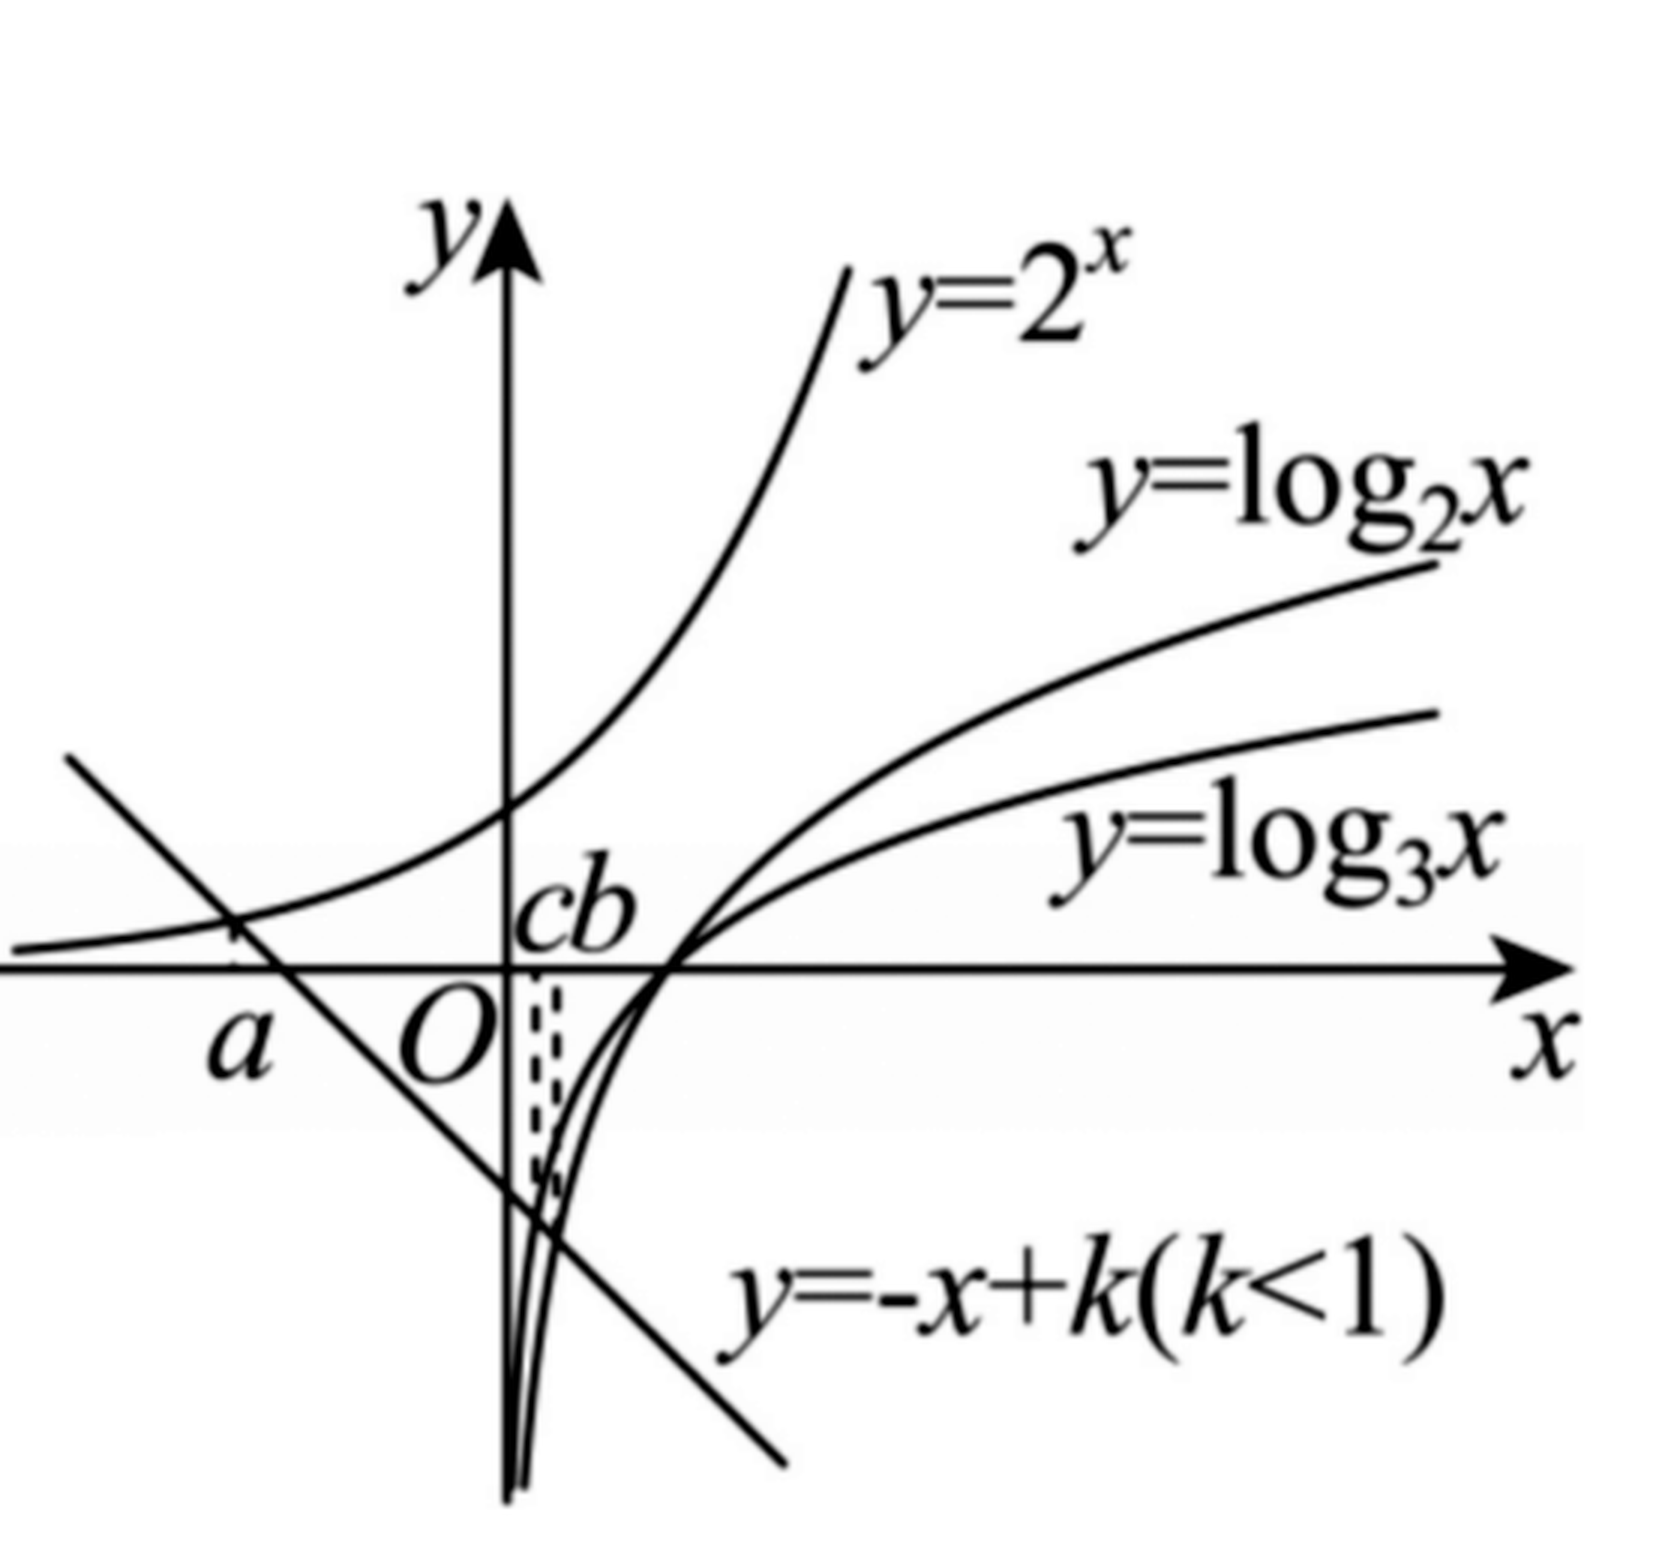
\includegraphics[width=0.52\textwidth]{figures/gao156_q15_curves.png}
\end{center}

\step{如图所示，由图象得 $a<c<b$. 故选 $B$.}
\solend
\fi

% === Q16 === ①② 文本圈数字、"一阶/二阶不动点""稳定点"自定义名词；解析 5 行，故选 A
\item 对定义域为 $I$ 的函数 $y=f(x)$，若存在 $x_0\in I$ 使得 $f(x_0)=x_0$，则称 $x_0$ 是函数 $f(x)$ 的
一阶不动点，简称不动点；若存在 $x_0\in I$ 使得 $f(f(x_0))=x_0$，则称 $x_0$ 是函数 $f(x)$ 的二阶
不动点，简称稳定点. 现有如下两个命题：①存在函数非 $y=x$ 且有无穷多个不动点；②
存在函数有无穷多个稳定点，且这些稳定点不都是不动点. 则\mbox{（\quad）}

\keepwithprev
A. ①成立，②成立\qquad\qquad B. ①成立，②不成立

C. ①不成立，②成立\qquad\qquad D. ①不成立，②不成立

\ifanswer
\solbegin
\step{①取定义在全体实数上的 $f(x)=\lvert x\rvert$，其不动点为一切非负实数，有无穷多个，}
\step{且 $f(-1)=1\ne-1$，①成立.}
\step{②取定义在全体实数上的 $g(x)=-x$，则 $g(g(x))=-(-x)=x$，}
\step{全体实数都是稳定点，而不动点只有 0，②成立.}
\step{故选 $A$.}
\solend
\fi

\end{enumerate}

\bigsec{三、解答题}

\begin{enumerate}
\setcounter{enumi}{16}

% === Q17 === $A\cap B$、$B\cap C$、\varnothing、\mid；解析 6 行
\item 设集合 $A=\{x\mid-1\leqslant x\leqslant2\}$，$B=\{x\mid2m<x<1\}$，$C=\{x\mid x<-1$ 或 $x>2\}$.

(1) 若 $A\cap B=B$，求实数 $m$ 的取值范围；

(2) 若 $B\cap C$ 中只有一个整数，求实数 $m$ 的取值范围.

\ifanswer
\solbegin
\step{(1) 当 $m\geqslant\dfrac12$ 时，$B=\varnothing$，满足 $A\cap B=B$.}
\step{当 $m<\dfrac12$ 时，$A\cap B=B$ 等价于 $2m\geqslant-1$，得 $-\dfrac12\leqslant m<\dfrac12$.}
\step{因此 $m$ 的取值范围为 $\left[-\dfrac12,+\infty\right)$.}
\step{(2) $B\cap C=\{x\mid2m<x<-1\}$，其中只有一个整数时，该整数必为 $-2$.}
\step{包含 $-2$ 且不包含 $-3$，等价于 $-3\leqslant2m<-2$，}
\step{因此 $m$ 的取值范围为 $\left[-\dfrac32,-1\right)$.}
\solend
\fi

% === Q18 === 幂函数 $x^{-\frac13}$、$m\in\R$；解析 12 行，跨 05—06 页
\item 已知幂函数 $f(x)=(3m^2-2m)x^m$（$m\in\R$）在定义域上不单调.

(1) 求函数 $f(x)$ 的解析式；

(2) 若 $f(a+1)<f(-2a+3)$，求实数 $a$ 的取值范围.

\ifanswer
\solbegin
\step{(1) 由幂函数的定义，$3m^2-2m=1$，即 $(3m+1)(m-1)=0$，得 $m=1$ 或 $m=-\dfrac13$.}
\step{当 $m=1$ 时，$f(x)=x$ 在定义域上单调递增，不合题意.}
\step{当 $m=-\dfrac13$ 时，$f(-1)=-1<f(1)=1$，而 $f(1)=1>f(8)=\dfrac12$，}
\step{故 $f(x)$ 在定义域上不单调.}
\step{因此 $f(x)=x^{-\frac13}$，定义域为 $(-\infty,0)\cup(0,+\infty)$.}
\step{(2) 有意义的条件为 $a\ne-1$ 且 $a\ne\dfrac32$.}
\step{当 $a<-1$ 时，$a+1<0<-2a+3$，有 $f(a+1)<0<f(-2a+3)$，}
\step{不等式成立.}
\step{当 $-1<a<\dfrac32$ 时，利用 $f(x)$ 在 $(0,+\infty)$ 上单调递减，}
\step{原不等式等价于 $a+1>-2a+3$，得 $\dfrac23<a<\dfrac32$.}
\step{当 $a>\dfrac32$ 时，$f(a+1)>0>f(-2a+3)$，不等式不成立.}
\step{所以 $a\in(-\infty,-1)\cup\left(\dfrac23,\dfrac32\right)$.}
\solend
\fi

% === Q19 === 两套解法（法一红字 \stepm，法二无标签）；\Delta 与 \subseteq；解析 21 行，跨 06—08 页
\item 已知 $a,c\in\R$，函数 $f(x)=\dfrac{x^2+(3a+1)x+c}{x+a}$.

(1) 若 $a=0$，求函数的定义域，并判断是否存在 $c$ 使得 $y=f(x)$ 图像关于原点对称，说明理由；

(2) 若函数过点 $(1,3)$，且函数 $y=f(x)$ 与 $x$ 轴负半轴有两个不同交点，求此时 $c$ 的值和 $a$ 的取值范围.

\ifanswer
\solbegin
\step{(1) 当 $a=0$ 时，$f(x)=\dfrac{x^2+(3a+1)x+c}{x+a}=\dfrac{x^2+x+c}{x}=x+\dfrac cx+1$，}
\step{故定义域为 $(-\infty,0)\cup(0,+\infty)$；}
\step{若存在实数 $c$，使得函数 $f(x)$ 为奇函数，则必有 $f(x)+f(-x)=0$，}
\step{而 $x+\dfrac cx+1+(-x)+\dfrac c{-x}+1=2\ne0$，}
\step{所以不存在实数 $c$，使得函数 $f(x)$ 为奇函数；}
\step{(2) 函数 $f(x)$ 的图像过点 $(1,3)$，则 $f(1)=\dfrac{1+(3a+1)+c}{1+a}=\dfrac{3a+c+2}{a+1}=3$，}
\step{解得 $c=1$，所以 $f(x)=\dfrac{x^2+(3a+1)x+1}{x+a}$，}
\stepm{法一：}{令 $f(x)=0$，则 $x^2+(3a+1)x+1=0$，此时方程有两不等负根，}
\step{则有 $\begin{cases}\Delta=(3a+1)^2-4>0\\-(3a+1)<0\end{cases}\Rightarrow\begin{cases}a>\dfrac13\text{ 或 }a<-1\\a>-\dfrac13\end{cases}\Rightarrow a>\dfrac13$，}
\step{注意到分母 $x+a\ne0$，则 $x\ne-a$，}
\step{若 $x=-a$ 也是方程 $x^2+(3a+1)x+1=0$ 的解，}
\step{代入方程 $(-a)^2+(3a+1)(-a)+1=0\Rightarrow2a^2+a-1=(a+1)(2a-1)=0$，}
\step{解得 $a=-1$ 或 $a=\dfrac12$，从而 $a\ne\dfrac12$，}
\step{综上，实数 $a$ 的取值范围为 $\left(\dfrac13,\dfrac12\right)\cup\left(\dfrac12,+\infty\right)$.}
\step{令 $g(x)=x^2+(3a+1)x+1$，与 $x$ 轴负半轴有两个交点，}
\step{则 $\begin{cases}-(3a+1)<0\\\Delta=(3a+1)^2-4>0\end{cases}\Rightarrow a>\dfrac13$.}
\step{注意到分母 $x+a\ne0$，则 $x\ne-a$，}
\step{若 $x=-a$ 也是方程 $x^2+(3a+1)x+1=0$ 的解，}
\step{代入方程 $(-a)^2+(3a+1)(-a)+1=0\Rightarrow2a^2+a-1=(a+1)(2a-1)=0$，}
\step{解得 $a=-1$ 或 $a=\dfrac12$，从而 $a\ne\dfrac12$，}
\step{综上，实数 $a$ 的取值范围为 $\left(\dfrac13,\dfrac12\right)\cup\left(\dfrac12,+\infty\right)$.}
\solend
\fi

% === Q20 === $Q$ 常数段 80000 照录；cases 与基本不等式；解析 10 行，跨 08—09 页
\item 某工厂生产某种零件的固定成本为 20000 元，每生产一个零件要增加投入 100 元，已知
总收入 $Q$（单位：元）关于产量 $x$（单位：个）满足函数：$Q=\begin{cases}400x-\dfrac12x^2,&0\leqslant x\leqslant400\\80000,&x>400\end{cases}$.

(1) 将利润 $P$（单位：元）表示为产量 $x$ 的函数；（总收入$=$总成本$+$利润）

(2) 当产量为何值时，零件的单位利润最大？最大单位利润是多少元？（单位利润$=$利润$\div$产量）

\ifanswer
\solbegin
\step{(1) 当 $0\leqslant x\leqslant400$ 时，}
\step{$P(x)=400x-\dfrac12x^2-20000-100x=-\dfrac12x^2+300x-20000$，}
\step{当 $x>400$ 时，$P(x)=80000-100x-20000=60000-100x$，}
\step{故 $P(x)=\begin{cases}-\dfrac12x^2+300x-20000,&0\leqslant x\leqslant400\\60000-100x,&x>400\end{cases}$.}
\step{(2) 设零件的单位利润为 $g(x)$，则 $g(x)=\begin{cases}-\dfrac12x-\dfrac{20000}{x}+300,&0\leqslant x\leqslant400\\\dfrac{60000}{x}-100,&x>400\end{cases}$，}
\step{当 $0\leqslant x\leqslant400$ 时，}
\step{$g(x)=300-\left(\dfrac12x+\dfrac{20000}{x}\right)\leqslant300-2\sqrt{\dfrac x2\cdot\dfrac{20000}{x}}=100$，}
\step{当且仅当 $\dfrac x2=\dfrac{20000}{x}$，即 $x=200$ 时取等号，}
\step{当 $x>400$ 时，$g(x)=\dfrac{60000}{x}-100$，此时无最值，}
\step{故当产量为 200 个，零件的单位利润最大，最大单位利润是 100 元.}
\solend
\fi

% === Q21 === 上升集定义、$D(x_0)=\{d\in\R\mid\cdots\}$、①②③ 文本圈数字、
%            \subseteq 带下划线、$-2^{-x}$；解析 19 行，跨 09—10 页
\item 已知函数 $y=f(x)$ 的定义域为 $\R$. 对任意 $x_0\in\R$，定义集合
$D(x_0)=\{d\in\R\mid f(x_0+d)>f(x_0)\}$，则称 $D(x_0)$ 为函数 $y=f(x)$ 在 $x_0$ 处的上升集.

(1) 若 $f(x)=1-x$，求 $D(-1)$；

(2) 若 $f(x)=\begin{cases}2^x,&x<0\\0,&x=0\\-2^{-x},&x>0\end{cases}$，求 $D(x)$；

(3) 设 $y=f(x)$ 满足：①当 $x<0$ 时，$f(x)=2^x$；②若 $f(x_1)\leqslant f(x_2)$，则
$D(x_2)\subseteq D(x_1)$；③当 $0<x<1$ 时，$f(x)<f(0)$. 证明：$f(0)\geqslant1$.

\ifanswer
\solbegin
\step{(1) $f(-1+d)>f(-1)\Leftrightarrow2-d>2\Leftrightarrow d<0$，所以 $D(-1)=(-\infty,0)$.}
\step{(2) 函数在 $(-\infty,0)$、$(0,+\infty)$ 上分别严格递增，}
\step{且这两个区间上的函数值分别为正、负，$f(0)=0$.}
\step{当 $x<0$ 时，$f(x+d)>f(x)\Leftrightarrow x<x+d<0\Leftrightarrow0<d<-x$，}
\step{当 $x=0$ 时，$f(d)>f(0)\Leftrightarrow d<0$，}
\step{当 $x>0$ 时，$f(x+d)>f(x)\Leftrightarrow x+d\leqslant0$ 或 $x+d>x$}
\step{$\Leftrightarrow d\leqslant-x$ 或 $d>0$，}
\step{因此 $D(x)=\begin{cases}(0,-x),&x<0\\(-\infty,0),&x=0\\(-\infty,-x]\cup(0,+\infty),&x>0\end{cases}$.}
\step{(3) 任取 $a\in(-1,0)$，}
\step{令 $d=-\dfrac a2$，则 $0<d<1$，且 $f(a+d)=2^{\frac a2}>2^a=f(a)$，}
\step{所以 $d\in D(a)$；}
\step{由③，$f(d)<f(0)$，所以 $d\notin D(0)$.}
\step{若 $f(0)\leqslant f(a)$，由②得 $D(a)\subseteq D(0)$，与上述结论矛盾.}
\step{因此，对任意 $a\in(-1,0)$，都有 $f(0)>2^a$.}
\step{特别地 $f(0)>2^{-\frac12}>0$.}
\step{若 $f(0)<1$，取 $a=\dfrac12\log_2 f(0)$，则 $-\dfrac14<a<0$，且}
\step{$2^a=\sqrt{f(0)}>f(0)$，}
\step{与 $f(0)>2^a$ 矛盾.}
\step{所以 $f(0)\geqslant1$.}
\solend
\fi

\end{enumerate}

\end{document}
"
%
% ① 原始材料：微信公众号"魔都数学加油站"文章，连载"27学年高一156"，原文标题
% "27学年高一156——2026-2027年上海市大同中学高一上期中"；
% 原文链接：https://mp.weixin.qq.com/s/xLtS5tyjCPJIWCIBohwGvw 。
% 正文为 10 张 PNG 页（01/02/03/04/05/06/07/08/09/10 各页分辨率混排
% 2560×3620 与 4762×6735，逐页按各自分辨率裁图核对）。
% 体例：讲评版——填空 3—12（10 题）、选择 13—16（4 题）、解答 17—21（5 题），
% 共 19 题，自第 3 题起编（1、2 未印在本篇）；Q3 只印【答案】、其余 18 题
% 逐题印【解析】（逐题核实，见 ②）。题目、答案、解析均据原图转录；卷面粉红色
% 水印"魔都数学加油站"及公众号页脚未录入。
%
% 卷首标题：原卷印作"2026-2027 年大同中学高一上期中"，年份区间按全稿惯例排 en dash；
% 原卷卷面未印副标题，本稿按同期中卷知识模块口径补出"集合与常用逻辑用语、不等式、函数"。
%
% ② 与原卷的排版差异：
%   ① 原文从第 3 题起，本稿保留原题号；共 19 题三节，解答题 5 题到 21；
%   ② 混合体例：第 3 题只印【答案】、无【解析】，按 高一140 第 5 题／高一145
%      第 3 题／高一151 第 7 题成例另提 \ans{}、不补造解析；其余 18 题印
%      【解析】、用 \solbegin…\solend；四道选择题答案在解析末句"故选 C／C／B／A"
%      （逐个放大复核）、括号 \mbox{（\quad）} 留空、不另提 \ans{}；答案版
%      【答案】/【解析】标记数 = 19 = 全卷题数（1 个 \ans ＋ 18 个 \solbegin）；
%   ③ 原卷卷面未印副标题，本稿按知识模块口径补出；
%   ④ 原卷填空横线按全稿惯例排 \blankline[4.4em]；选择题括号排 \mbox{（\quad）}、
%      选项段前按惯例各加 \keepwithprev；解答题不留作答区、不加 \anspace
%      （原卷为讲评版，109—113 起全稿不用 \anspace）；
%   ⑤ 数集：Q3"$x\in\R$"、Q18"$m\in\R$"、Q19"$a,c\in\R$"、Q21"定义域为 \R"
%      "任意 $x_0\in\R$""$d\in\R$"原卷印正体粗体 R，按全稿惯例归一 \R；
%      绝对值排 \lvert…\rvert（Q11 $\lvert2^x-1\rvert$、Q16 $\lvert x\rvert$），
%      集合描述竖线排 \mid（Q17 $A=\{x\mid\cdots\}$、Q21 $D(x_0)=\{d\in\R\mid\cdots\}$），
%      空集 \varnothing（Q17"$B=\varnothing$"），不等号按全稿惯例排 \leqslant／\geqslant；
%   ⑥ 子集符号逐处照录不统一：Q21 (3) 题干"$D(x_2)\subseteq D(x_1)$"与解析
%      "$D(a)\subseteq D(0)$"均印带下划线 ⊆，照录 \subseteq；本卷无单线 ⊂ 用例；
%   ⑦ 判别式：Q19 两套解法"$\Delta=(3a+1)^2-4>0$"印等腰偏高 \Delta，照录 \Delta；
%      本卷无扁三角 \triangle 用例；
%   ⑧ 红字照录为黑体：Q19 (2) 解析第一套解法行首"法一："原卷排**红色加粗**，
%      按 高一53 成例排 \stepm{法一：}{…}（加粗着色、不改黑色基调），全库无红字
%      排字先例、本稿不引入红色定义，文件头注明；第二套解法原卷直接以
%      "令 $g(x)=x^2+(3a+1)x+1$，与 $x$ 轴负半轴有两个交点，"另起，
%      **未印"法二："标签**（逐页像素级复核：07 页仅 1437—1475 一处红字，
%      08 页无红字），照录为普通 \step、不补造标签；
%   ⑨ 文本模式圈数字逐处照录：Q12 解析 ①② 两情形、Q16 两则命题与四个选项及
%      解析的 ①②、Q21 (3) 三条件 ①②③ 与解析"由③""由②"，均为印刷圈数字
%      （非 \textcircled、非数学模式），计入圈数字实测；
%   ⑩ 自定义名词照录：Q16"一阶不动点，简称不动点""二阶不动点，简称稳定点"、
%      Q21"上升集"；Q16 题干"存在函数非 $y=x$ 且有无穷多个不动点"照录；
%   ⑪ 中文弯引号照录：Q3""存在 $x\in\R$，$x^3-1\leqslant0$" 否定形式为"、
%      Q13"使"$\dfrac{x+1}{1-x}\geqslant0$"成立的必要不充分条件是"；
%      注释里一律 ASCII 引号；数学式内 CJK 用 \text{}（Q19 cases 内"或"）；
%   ⑫ 半角逗号在数学组之间是全稿惯例、非笔误，逐处照录（$a,c$、$x,y$、$a,b$
%      之类）；行末西文句点 ASCII `.`；行中全角逗号／顿号照录；
%   ⑬ 复杂式照录别简化：Q6 $\left(\dfrac{1}{\sqrt a}\right)^{\frac27}\cdot\sqrt[7]{a^3}$
%      与解析 $a^{\frac{12}{7}-\frac17+\frac37}$、Q8 $2\sqrt4+5=9$（$\sqrt4$ 未化简）、
%      Q9 $\left(\sqrt x+\dfrac{1}{\sqrt x}\right)^3$、Q12 $\dfrac{4a-(2-a)^2}{4a}$、
%      Q18 $f(8)=\dfrac12$、Q19 $2a^2+a-1=(a+1)(2a-1)=0$、Q20 $Q$ 的常数段
%      $80000$（不是 $80000-100x$）与 $2\sqrt{\dfrac x2\cdot\dfrac{20000}{x}}$、
%      Q21 $f(a+d)=2^{\frac a2}>2^a=f(a)$ 与 $2^a=\sqrt{f(0)}>f(0)$ 等；
%      \left…\right 不得拆到不同 $…$ 组（Q5 $\left(0,\dfrac12\right)$、
%      Q12 $\left[0,4+2\sqrt3\right)$、Q17 $\left[-\dfrac12,+\infty\right)$、
%      Q19 $\left(\dfrac13,\dfrac12\right)\cup\left(\dfrac12,+\infty\right)$、
%      Q20 $\left(\dfrac12x+\dfrac{20000}{x}\right)$ 等）；cases 块整体算一个印刷行；
%   ⑭ 一条 \step = 原卷解析的一个印刷行；别并折行、别拆行。跨页续印按题合并
%      （Q6 的 01 页上下题干重复印、Q8 的 01—02 页、Q12 的 02—03 页、
%      Q15 的 04 页上下、Q16 的 04—05 页、Q17 的 05 页上下、Q18 的 05—06 页、
%      Q19 的 06—08 页、Q20 的 08—09 页、Q21 的 09—10 页）；
%      跨半页重叠行（Q12 的"②若 …"、Q18 的"原不等式等价于 …"、
%      Q20 的"【解析】(1) 当 $0\leqslant x\leqslant400$ 时，"、Q21 的
%      "【解析】(1) $f(-1+d)>f(-1)\cdots$"与"与 $f(0)>2^a$ 矛盾."）
%      只算一个印刷行；
%   ⑮ 配图：全卷 3 组（逐页通读 10 页确认）——
%      · Q14 题干 S-t 梯形图（03 页右下，离家距离 S 对行走时间 t），题目配图、
%        三版都出，裁 figures/gao156_q14_st.png；
%      · Q14 四幅路线选项（04 页上部，A/B/C/D 四幅横排、C 为以家为圆心的圆弧），
%        题目配图、三版都出，合并成一张，裁 figures/gao156_q14_opts.png；
%      · Q15 解析内曲线交点图（04 页右下，$y=2^x$、$y=\log_2x$、$y=\log_3x$
%        与 $y=-x+k$），仅答案版出，裁 figures/gao156_q15_curves.png；
%      3 图均取自原卷截图，去粉色水印、去色、3×~4× LANCZOS 放大；
%      Q14 题干"题干＋两图"整块用 \needvspace 守卫推走（守卫放 \item 之前，
%      见 高一154 Q15／高一136 Q13 成例）；Q15 解析内图放 \ifanswer 内
%      \solbegin…\solend 的两 \step 之间（高一108 第 6 题／高一154 附加题 2 成例）；
%      其余各页逐页确认无其它题目配图、无解析配图、无表格；10 页下半仅水印、无正文。
%
% ③ 行数复核：一条 \step = 原卷解析的一个印刷行，cases 块作一个印刷行计。
%   逐题数（主会话逐页核对定稿）：Q3：0（只印【答案】、提 \ans{}，不计入 \step 账）；
%   Q4：1；Q5：1；Q6：1；Q7：1；Q8：3；Q9：2；Q10：2；Q11：5；Q12：12；
%   Q13：3；Q14：3；Q15：4；Q16：5；Q17：6；Q18：12；Q19：21；Q20：10；Q21：19。
%   合计 111 行（110 条 \step ＋ 1 条 \stepm），与原卷逐题印刷行相等。
%   全卷 19 题：Q3 一处 \ans{} ＋ 其余 18 题设 \solbegin…\solend，
%   答案版【答案】/【解析】标记数 = 19 = 全卷题数。
%
% ④ 页码分布（供回原图复核）：
%   卷首标题＋"一、填空题"＋Q3 题干＋【答案】、Q4 题干＋解析 1 行、
%   Q5 题干＋解析 1 行、Q6 题干首行在 01 页上半；
%   Q6 题干（重复印）＋解析 1 行、Q7 题干＋解析 1 行、Q8 题干＋解析前 2 行
%   在 01 页下半；Q8 解析末行、Q9 题干＋解析 2 行、Q10 题干＋解析 2 行、
%   Q11 题干首行在 02 页上半；Q11 题干（重复印）＋解析 5 行、
%   Q12 题干＋解析首行在 02 页下半；Q12 解析中 9 行在 03 页上半；
%   Q12 解析末 2 行＋"二、选择题"标题＋Q13 题干＋选项＋解析 3 行＋
%   Q14 题干首行在 03 页下半；Q14 题干续行＋四幅选项图＋解析 3 行＋
%   Q15 题干＋选项＋解析前 2 行＋Q16 题干在 04 页上半；
%   Q15 解析后 2 行＋曲线图＋Q16 选项＋解析前 2 行在 04 页下半；
%   Q16 解析后 3 行＋"三、解答题"标题＋Q17 题干＋两问＋解析 (1) 3 行
%   在 05 页上半；Q17 解析 (2) 3 行＋Q18 题干＋两问＋解析 (1) 首 2 行
%   在 05 页下半；Q18 解析 (1)(2) 中 8 行在 06 页上半；Q18 解析末 2 行＋
%   Q19 题干＋两问＋解析 (1) 首行在 06 页下半；Q19 解析 (1) 后 4 行＋
%   (2) 前 2 行＋法一 2 行在 07 页上半；法一后 5 行＋法二前 3 行在 07 页下半；
%   法二后 4 行＋Q20 题干＋两问＋解析 (1) 首行在 08 页上半；
%   Q20 解析 (1) 后 3 行＋(2) 前 5 行在 08 页下半；Q20 解析 (2) 末 2 行＋
%   Q21 题干＋三问＋解析 (1) 首行在 09 页上半；Q21 解析 (1)（重复印）＋
%   (2) 8 行＋(3) 首行在 09 页下半；Q21 (3) 解析中 8 行在 10 页上半；
%   Q21 (3) 末 2 行在 10 页下半。本稿按题连排，不丢行、不并折行；
%   全卷末题为第 21 题，无附加题节。
%
\documentclass[a4paper,11pt]{article}
\usepackage{common}

\begin{document}

\examtitlest[3]{2026--2027 年大同中学高一上期中}{集合与常用逻辑用语、不等式、函数}

\bigsec{一、填空题}

\begin{enumerate}
\setcounter{enumi}{2}

% === Q3 === 只印【答案】、无【解析】；R 正体粗体 \R；中文弯引号照录
\item “存在 $x\in\R$，$x^3-1\leqslant0$” 否定形式为\blankline[4.4em].

\ifanswer
\ans{对任意 $x\in\R$，$x^3-1>0$}
\fi

% === Q4 === 解析 1 行
\item 若实数 $a>0$ 且 $a\ne1$，函数 $y=a^{x-3}+1$ 的图像恒过定点 $P$，则点 $P$ 的坐标为\blankline[4.4em].

\ifanswer
\solbegin
\step{当 $x=3$ 时，$y=a^0+1=2$，与 $a$ 无关，所以定点为 $P(3,2)$.}
\solend
\fi

% === Q5 === 解析 1 行
\item 函数 $y=\dfrac{1}{3^x+2}$ 的值域是\blankline[4.4em].

\ifanswer
\solbegin
\step{$3^x\in(0,+\infty)$，因此 $3^x+2\in(2,+\infty)$，值域为 $\left(0,\dfrac12\right)$.}
\solend
\fi

% === Q6 === 根式嵌套照录；解析 1 行；题干跨 01 页上下重复印
\item 已知 $a>0$，化简 $a^{\frac{12}{7}}\cdot\left(\dfrac{1}{\sqrt a}\right)^{\frac27}\cdot\sqrt[7]{a^3}=$\blankline[4.4em].

\ifanswer
\solbegin
\step{原式 $=a^{\frac{12}{7}}\cdot a^{-\frac17}\cdot a^{\frac37}=a^{\frac{12}{7}-\frac17+\frac37}=a^2$.}
\solend
\fi

% === Q7 === 换底公式；解析 1 行
\item 已知 $\log_5 3=a$，用 $a$ 的代数式表示 $\log_{15}125=$\blankline[4.4em].

\ifanswer
\solbegin
\step{$\log_{15}125=\dfrac{\log_5 125}{\log_5 15}=\dfrac{3}{1+\log_5 3}=\dfrac{3}{1+a}$.}
\solend
\fi

% === Q8 === 基本不等式，$\sqrt4$ 照录未化简；解析 3 行，跨 01—02 页
\item 已知 $x>0$，$y>0$，且 $4x+y=xy$，则 $x+y$ 的最小值为\blankline[4.4em].

\ifanswer
\solbegin
\step{由 $4x+y=xy$，得 $\dfrac4y+\dfrac1x=1$，}
\step{则 $x+y=(x+y)\left(\dfrac4y+\dfrac1x\right)=\dfrac{4x}{y}+\dfrac yx+1+4\geqslant2\sqrt4+5=9$，}
\step{当且仅当 $\dfrac{4x}{y}=\dfrac yx$，即 $x=3$，$y=6$ 时取等号，故最小值为 9.}
\solend
\fi

% === Q9 === 解析 2 行
\item 已知 $x^{-1}+x=7$（$x>0$），则 $x^{\frac32}+x^{-\frac32}$ 的值为\blankline[4.4em].

\ifanswer
\solbegin
\step{$x>0$，有 $\sqrt x+\dfrac{1}{\sqrt x}=\sqrt{x+\dfrac1x+2}=3$，}
\step{所以 $x^{\frac32}+x^{-\frac32}=\left(\sqrt x+\dfrac{1}{\sqrt x}\right)^3-3\left(\sqrt x+\dfrac{1}{\sqrt x}\right)=27-9=18$.}
\solend
\fi

% === Q10 === $x_{\min}$；解析 2 行
\item 已知不等式 $x>\dfrac{2a+1}{a-1}$ 对任意的 $x\in[1,2]$ 恒成立，则实数 $a$ 的取值范围是\blankline[4.4em].

\ifanswer
\solbegin
\step{不等式 $x>\dfrac{2a+1}{a-1}$ 对任意的 $x\in[1,2]$ 恒成立，得 $\dfrac{2a+1}{a-1}<x_{\min}=1$，}
\step{即有 $\dfrac{a+2}{a-1}<0$，解得 $-2<a<1$，则实数 $a$ 的取值范围是 $(-2,1)$.}
\solend
\fi

% === Q11 === 分段函数 cases 与绝对值 \lvert…\rvert；解析 5 行
\item 已知函数 $f(x)=\begin{cases}\lvert2^x-1\rvert-a,&x\leqslant2\\\dfrac{3}{x-1}-a,&x>2\end{cases}$，若函数 $y=f(x)$ 图像与 $x$ 轴有三个不同交点，则实数 $a$ 的取值范围是\blankline[4.4em].

\ifanswer
\solbegin
\step{令 $g(x)=f(x)+a$.}
\step{在 $(-\infty,0)$、$[0,2]$、$(2,+\infty)$ 上，$g(x)$ 均严格单调，}
\step{值域依次为 $(0,1)$、$[0,3]$、$(0,3)$.}
\step{每段至多有一个交点，因而恰有三个不同交点，}
\step{当且仅当 $a\in(0,1)\cap[0,3]\cap(0,3)=(0,1)$.}
\solend
\fi

% === Q12 === ①② 文本圈数字、对称轴与最小值式照录；解析 12 行，跨 02—03 页
\item 已知函数 $f(x)=ax^2-(2-a)x+1$，$g(x)=x$，若对于任意实数 $x$，$f(x)$ 与 $g(x)$ 至少有一个为正数，则实数 $a$ 的取值范围是\blankline[4.4em].

\ifanswer
\solbegin
\step{当 $x>0$ 时，$g(x)>0$；当 $x<0$ 时，$g(x)<0$；}
\step{当 $x=0$ 时，$f(0)=1>0$；}
\step{因为对于任意实数 $x$，$f(x)$ 与 $g(x)$ 至少有一个为正数，}
\step{当 $x<0$ 时，因为 $g(x)<0$，所以 $f(x)=ax^2-(2-a)x+1>0$ 恒成立，}
\step{当 $a<0$ 时，显然不成立，}
\step{当 $a=0$ 时，$f(x)=-2x+1>0$，对 $x<0$ 时恒成立，满足题意，}
\step{当 $a>0$ 时，函数图象开口向上，对称轴 $x=\dfrac{2-a}{2a}$，}
\step{①若 $\dfrac{2-a}{2a}\geqslant0$，即 $0<a\leqslant2$ 时，函数 $f(x)$ 在 $(-\infty,0)$ 上严格减，$f(0)=1$，}
\step{故 $f(x)>0$ 对 $x<0$ 时恒成立，满足题意；}
\step{②若 $\dfrac{2-a}{2a}<0$，即 $a>2$ 时，$f(x)_{\min}=f\left(\dfrac{2-a}{2a}\right)=\dfrac{4a-(2-a)^2}{4a}>0$，}
\step{解得 $4-2\sqrt3<a<4+2\sqrt3$，所以 $2<a<4+2\sqrt3$.}
\step{综上，$0\leqslant a<4+2\sqrt3$，故实数 $a$ 的取值范围是 $\left[0,4+2\sqrt3\right)$.}
\solend
\fi

\end{enumerate}

\bigsec{二、选择题}

\begin{enumerate}
\setcounter{enumi}{12}

% === Q13 === 必要不充分条件；cases 块；解析 3 行，故选 C
\item 使 “$\dfrac{x+1}{1-x}\geqslant0$” 成立的必要不充分条件是\mbox{（\quad）}

\keepwithprev
A. $-1\leqslant x<1$\qquad B. $x\leqslant-1$ 或 $x>1$\qquad C. $-1\leqslant x\leqslant1$\qquad D. $x\leqslant-1$ 或 $x\geqslant0$

\ifanswer
\solbegin
\step{由不等式 $\dfrac{x+1}{1-x}\geqslant0$ 得 $\begin{cases}(x+1)(1-x)\geqslant0\\1-x\ne0\end{cases}$，解得 $-1\leqslant x<1$，}
\step{由题意结合选项，$-1\leqslant x<1\Rightarrow-1\leqslant x\leqslant1$ 成立，反之不成立，}
\step{所以 $-1\leqslant x\leqslant1$ 是 $\dfrac{x+1}{1-x}\geqslant0$ 成立的必要不充分条件. 故选 $C$.}
\solend
\fi

% === Q14 === 题干 S-t 图＋四幅路线选项（题目配图，三版都出）；守卫放 \item 之前；解析 3 行，故选 C
\needvspace{9cm}
\item 如图是王老师锻炼时所走的离家距离（$S$）与行走时间（$t$）之间的函数关系图，若
用黑点表示王老师家的位置，则王老师行走的路线可能是\mbox{（\quad）}

\begin{center}
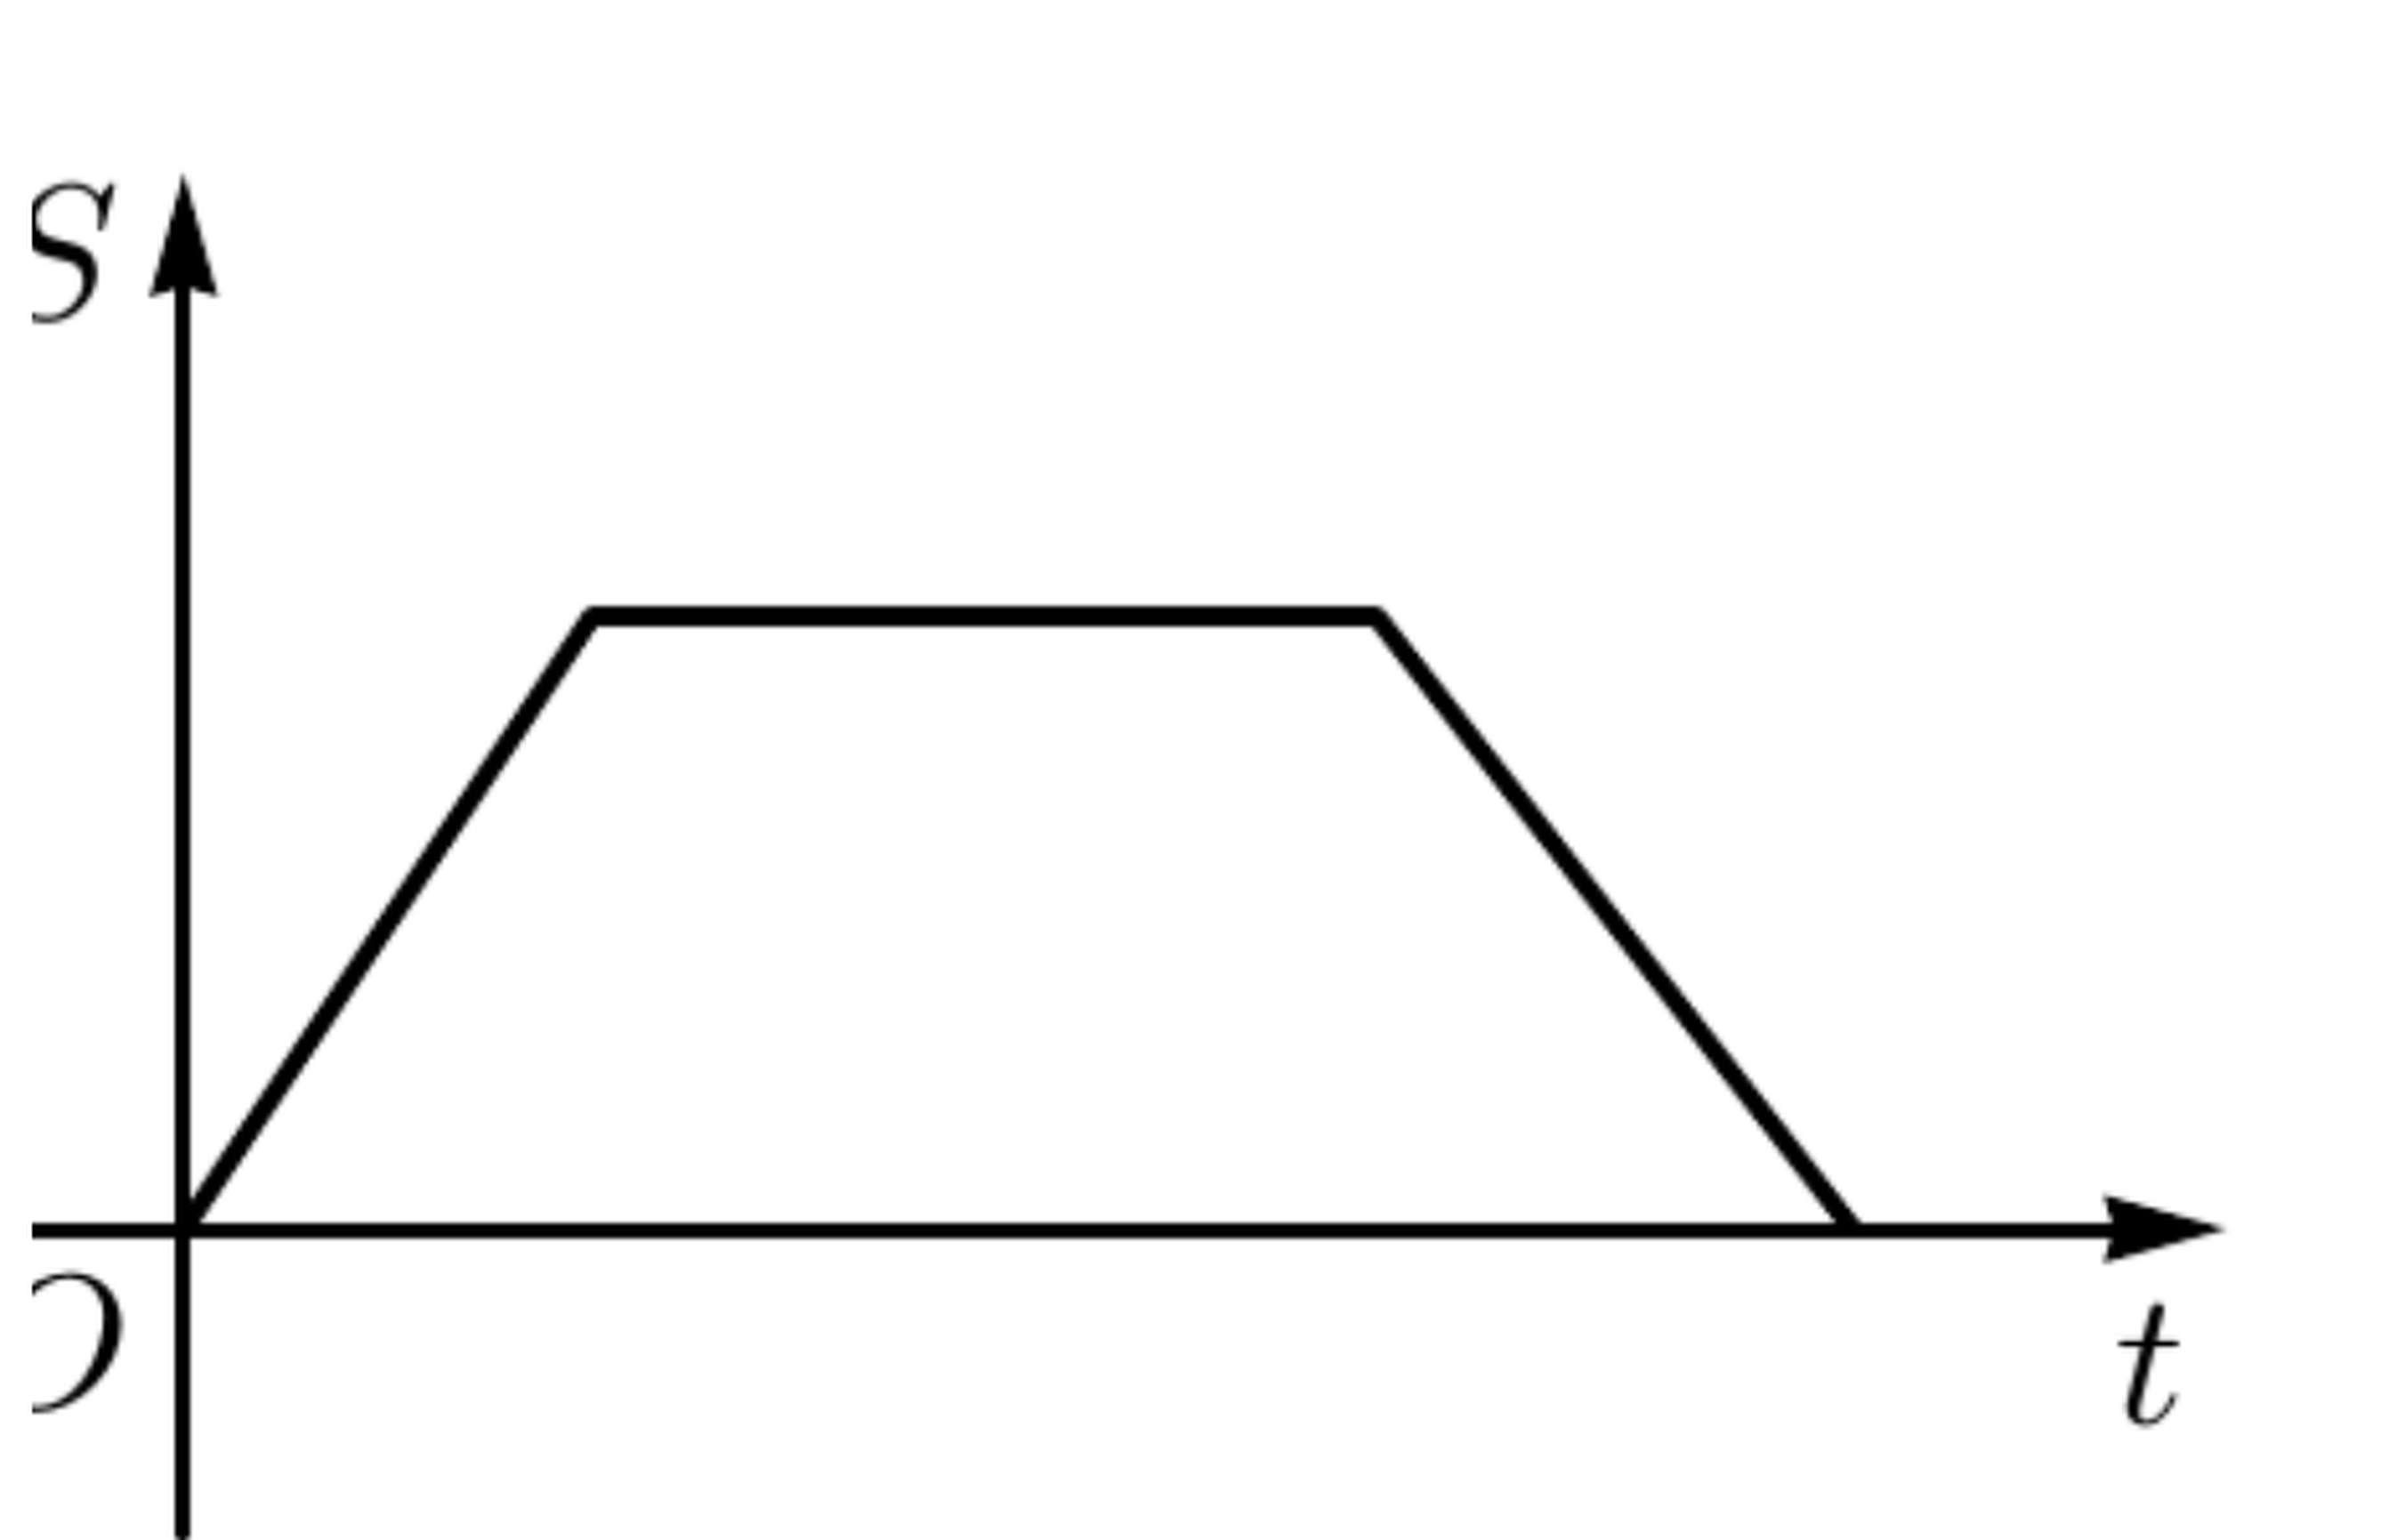
\includegraphics[width=0.34\textwidth]{figures/gao156_q14_st.png}
\end{center}

\keepwithprev
\begin{center}
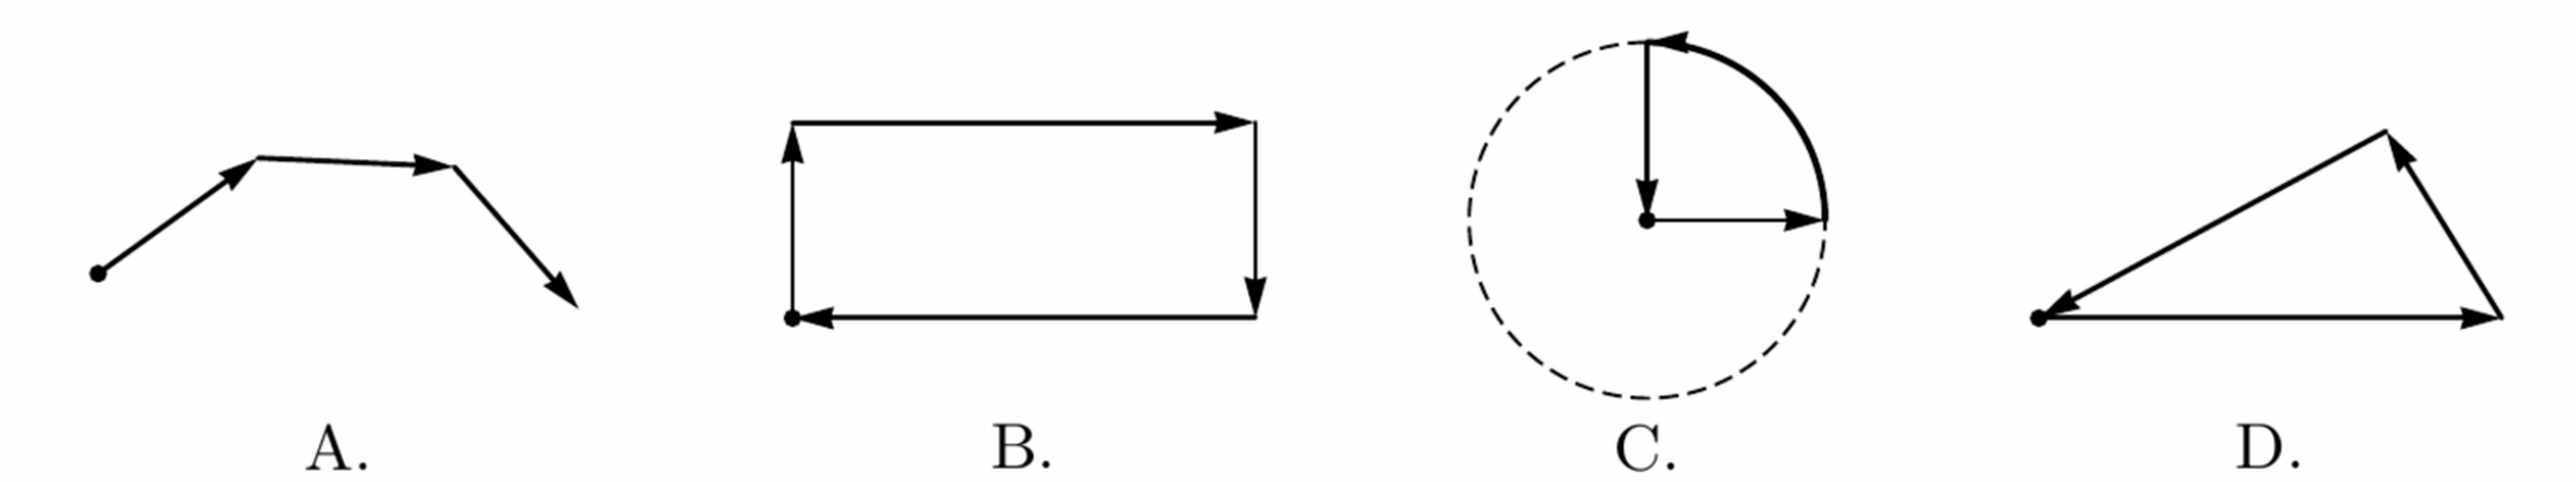
\includegraphics[width=0.86\textwidth]{figures/gao156_q14_opts.png}
\end{center}

\ifanswer
\solbegin
\step{由王老师锻炼时所走的离家距离（$S$）与行走时间（$t$）之间的函数关系图，}
\step{得在中间一段时间里，他到家的距离为定值，}
\step{故他所走的路程是一段以家为圆心的圆弧，故选 $C$.}
\solend
\fi

% === Q15 === 解析内曲线交点图（仅答案版出）；解析 4 行，故选 B
\item 已知 $a+2^a=b+\log_2 b=c+\log_3 c=k$，若 $k<1$，则\mbox{（\quad）}

\keepwithprev
A. $c<a<b$\qquad B. $a<c<b$\qquad C. $b<a<c$\qquad D. $a<b<c$

\ifanswer
\solbegin
\step{因为 $a+2^a=b+\log_2 b=c+\log_3 c=k$，}
\step{所以 $2^a=-a+k$，$\log_2 b=-b+k$，$\log_3 c=-c+k$，其中 $k<1$；}
\step{分别作出 $y=2^x$，$y=\log_2 x$，$y=\log_3 x$ 和 $y=-x+k$ 的图象，}

\begin{center}
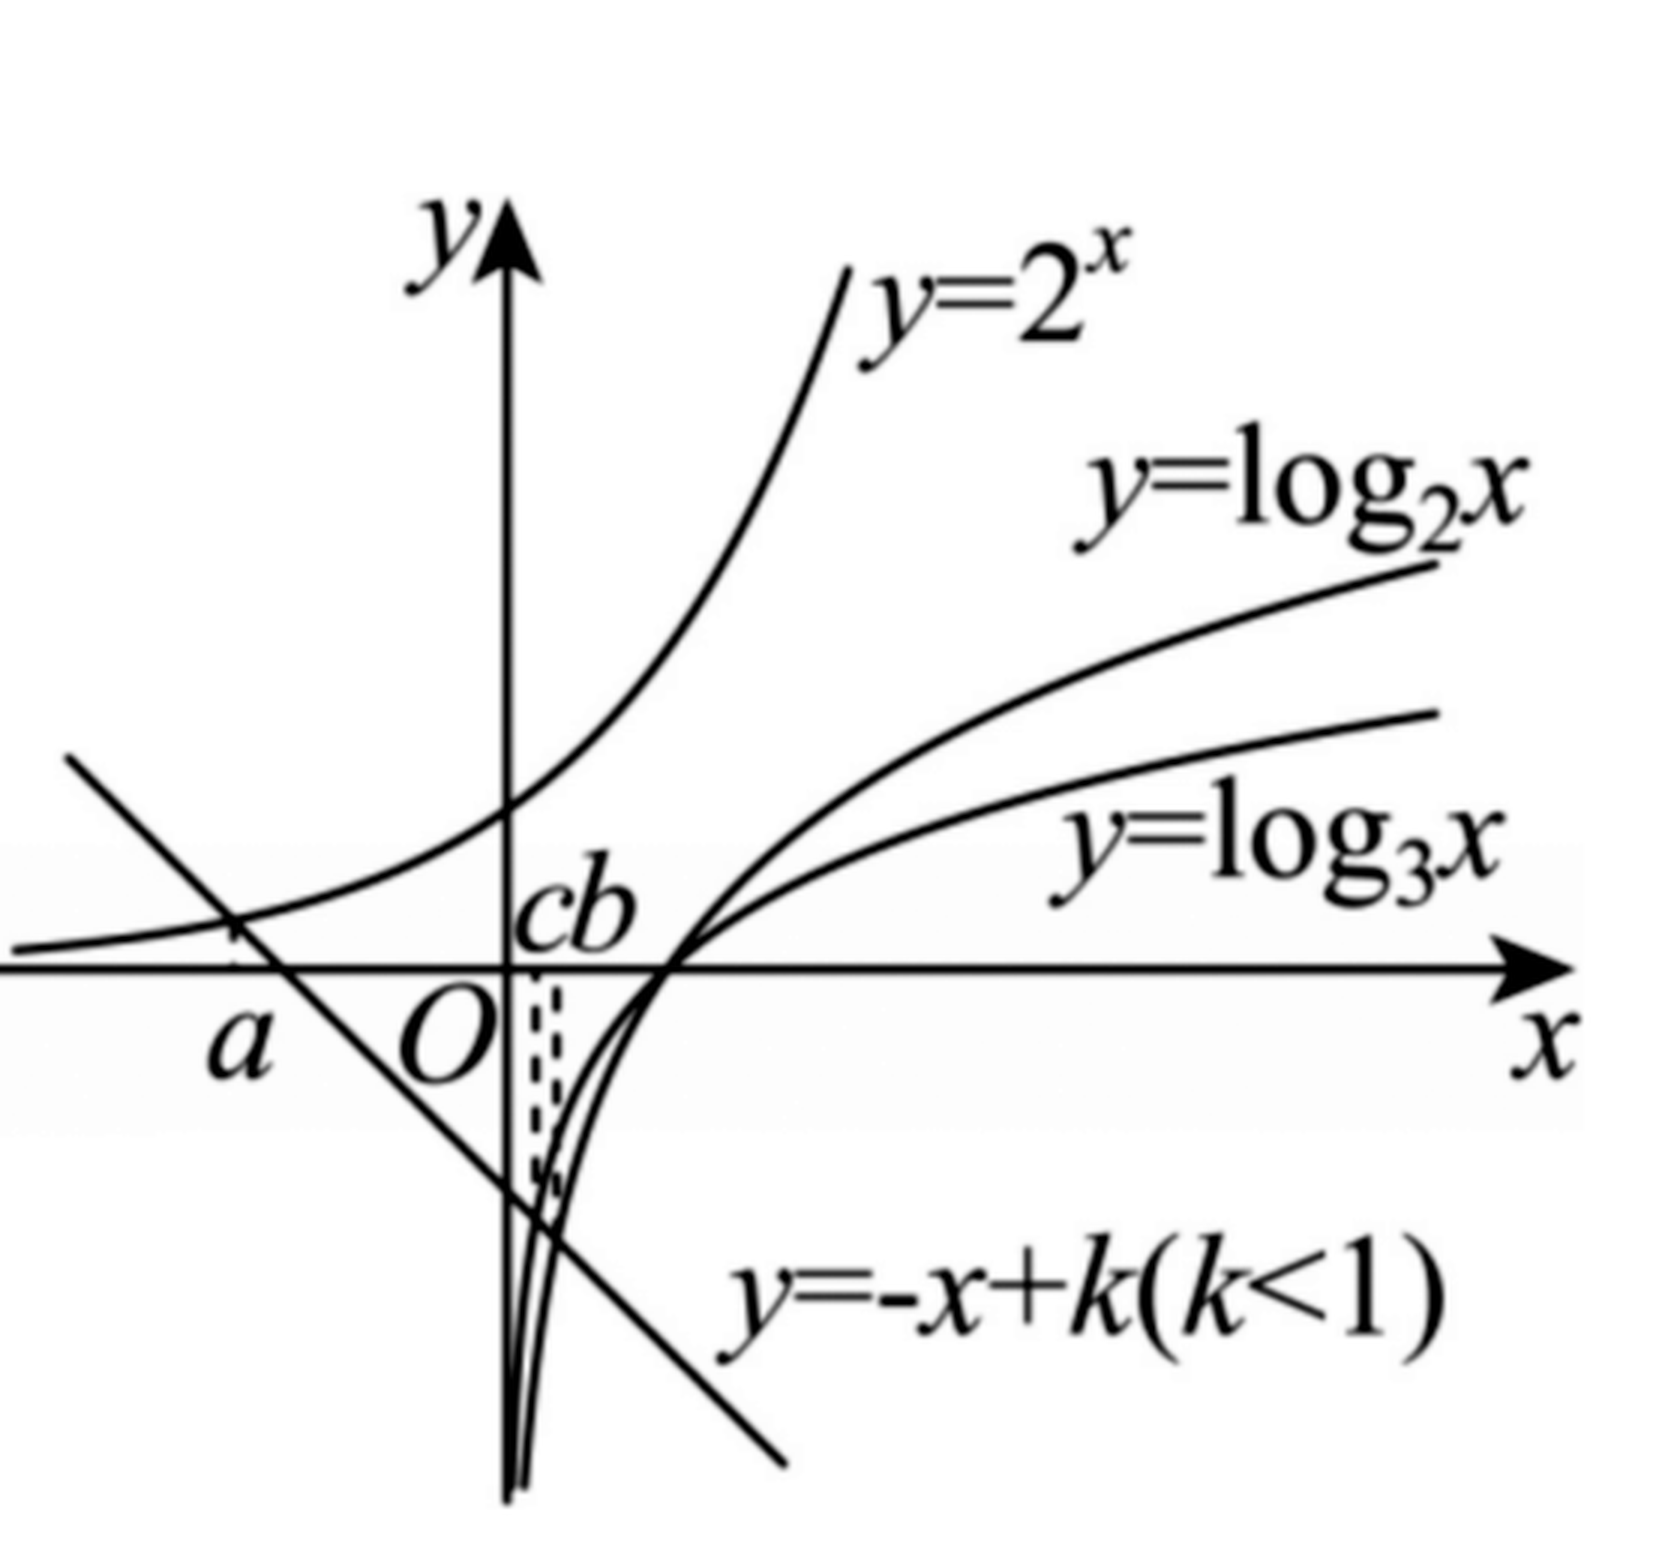
\includegraphics[width=0.52\textwidth]{figures/gao156_q15_curves.png}
\end{center}

\step{如图所示，由图象得 $a<c<b$. 故选 $B$.}
\solend
\fi

% === Q16 === ①② 文本圈数字、"一阶/二阶不动点""稳定点"自定义名词；解析 5 行，故选 A
\item 对定义域为 $I$ 的函数 $y=f(x)$，若存在 $x_0\in I$ 使得 $f(x_0)=x_0$，则称 $x_0$ 是函数 $f(x)$ 的
一阶不动点，简称不动点；若存在 $x_0\in I$ 使得 $f(f(x_0))=x_0$，则称 $x_0$ 是函数 $f(x)$ 的二阶
不动点，简称稳定点. 现有如下两个命题：①存在函数非 $y=x$ 且有无穷多个不动点；②
存在函数有无穷多个稳定点，且这些稳定点不都是不动点. 则\mbox{（\quad）}

\keepwithprev
A. ①成立，②成立\qquad\qquad B. ①成立，②不成立

C. ①不成立，②成立\qquad\qquad D. ①不成立，②不成立

\ifanswer
\solbegin
\step{①取定义在全体实数上的 $f(x)=\lvert x\rvert$，其不动点为一切非负实数，有无穷多个，}
\step{且 $f(-1)=1\ne-1$，①成立.}
\step{②取定义在全体实数上的 $g(x)=-x$，则 $g(g(x))=-(-x)=x$，}
\step{全体实数都是稳定点，而不动点只有 0，②成立.}
\step{故选 $A$.}
\solend
\fi

\end{enumerate}

\bigsec{三、解答题}

\begin{enumerate}
\setcounter{enumi}{16}

% === Q17 === $A\cap B$、$B\cap C$、\varnothing、\mid；解析 6 行
\item 设集合 $A=\{x\mid-1\leqslant x\leqslant2\}$，$B=\{x\mid2m<x<1\}$，$C=\{x\mid x<-1$ 或 $x>2\}$.

(1) 若 $A\cap B=B$，求实数 $m$ 的取值范围；

(2) 若 $B\cap C$ 中只有一个整数，求实数 $m$ 的取值范围.

\ifanswer
\solbegin
\step{(1) 当 $m\geqslant\dfrac12$ 时，$B=\varnothing$，满足 $A\cap B=B$.}
\step{当 $m<\dfrac12$ 时，$A\cap B=B$ 等价于 $2m\geqslant-1$，得 $-\dfrac12\leqslant m<\dfrac12$.}
\step{因此 $m$ 的取值范围为 $\left[-\dfrac12,+\infty\right)$.}
\step{(2) $B\cap C=\{x\mid2m<x<-1\}$，其中只有一个整数时，该整数必为 $-2$.}
\step{包含 $-2$ 且不包含 $-3$，等价于 $-3\leqslant2m<-2$，}
\step{因此 $m$ 的取值范围为 $\left[-\dfrac32,-1\right)$.}
\solend
\fi

% === Q18 === 幂函数 $x^{-\frac13}$、$m\in\R$；解析 12 行，跨 05—06 页
\item 已知幂函数 $f(x)=(3m^2-2m)x^m$（$m\in\R$）在定义域上不单调.

(1) 求函数 $f(x)$ 的解析式；

(2) 若 $f(a+1)<f(-2a+3)$，求实数 $a$ 的取值范围.

\ifanswer
\solbegin
\step{(1) 由幂函数的定义，$3m^2-2m=1$，即 $(3m+1)(m-1)=0$，得 $m=1$ 或 $m=-\dfrac13$.}
\step{当 $m=1$ 时，$f(x)=x$ 在定义域上单调递增，不合题意.}
\step{当 $m=-\dfrac13$ 时，$f(-1)=-1<f(1)=1$，而 $f(1)=1>f(8)=\dfrac12$，}
\step{故 $f(x)$ 在定义域上不单调.}
\step{因此 $f(x)=x^{-\frac13}$，定义域为 $(-\infty,0)\cup(0,+\infty)$.}
\step{(2) 有意义的条件为 $a\ne-1$ 且 $a\ne\dfrac32$.}
\step{当 $a<-1$ 时，$a+1<0<-2a+3$，有 $f(a+1)<0<f(-2a+3)$，}
\step{不等式成立.}
\step{当 $-1<a<\dfrac32$ 时，利用 $f(x)$ 在 $(0,+\infty)$ 上单调递减，}
\step{原不等式等价于 $a+1>-2a+3$，得 $\dfrac23<a<\dfrac32$.}
\step{当 $a>\dfrac32$ 时，$f(a+1)>0>f(-2a+3)$，不等式不成立.}
\step{所以 $a\in(-\infty,-1)\cup\left(\dfrac23,\dfrac32\right)$.}
\solend
\fi

% === Q19 === 两套解法（法一红字 \stepm，法二无标签）；\Delta 与 \subseteq；解析 21 行，跨 06—08 页
\item 已知 $a,c\in\R$，函数 $f(x)=\dfrac{x^2+(3a+1)x+c}{x+a}$.

(1) 若 $a=0$，求函数的定义域，并判断是否存在 $c$ 使得 $y=f(x)$ 图像关于原点对称，说明理由；

(2) 若函数过点 $(1,3)$，且函数 $y=f(x)$ 与 $x$ 轴负半轴有两个不同交点，求此时 $c$ 的值和 $a$ 的取值范围.

\ifanswer
\solbegin
\step{(1) 当 $a=0$ 时，$f(x)=\dfrac{x^2+(3a+1)x+c}{x+a}=\dfrac{x^2+x+c}{x}=x+\dfrac cx+1$，}
\step{故定义域为 $(-\infty,0)\cup(0,+\infty)$；}
\step{若存在实数 $c$，使得函数 $f(x)$ 为奇函数，则必有 $f(x)+f(-x)=0$，}
\step{而 $x+\dfrac cx+1+(-x)+\dfrac c{-x}+1=2\ne0$，}
\step{所以不存在实数 $c$，使得函数 $f(x)$ 为奇函数；}
\step{(2) 函数 $f(x)$ 的图像过点 $(1,3)$，则 $f(1)=\dfrac{1+(3a+1)+c}{1+a}=\dfrac{3a+c+2}{a+1}=3$，}
\step{解得 $c=1$，所以 $f(x)=\dfrac{x^2+(3a+1)x+1}{x+a}$，}
\stepm{法一：}{令 $f(x)=0$，则 $x^2+(3a+1)x+1=0$，此时方程有两不等负根，}
\step{则有 $\begin{cases}\Delta=(3a+1)^2-4>0\\-(3a+1)<0\end{cases}\Rightarrow\begin{cases}a>\dfrac13\text{ 或 }a<-1\\a>-\dfrac13\end{cases}\Rightarrow a>\dfrac13$，}
\step{注意到分母 $x+a\ne0$，则 $x\ne-a$，}
\step{若 $x=-a$ 也是方程 $x^2+(3a+1)x+1=0$ 的解，}
\step{代入方程 $(-a)^2+(3a+1)(-a)+1=0\Rightarrow2a^2+a-1=(a+1)(2a-1)=0$，}
\step{解得 $a=-1$ 或 $a=\dfrac12$，从而 $a\ne\dfrac12$，}
\step{综上，实数 $a$ 的取值范围为 $\left(\dfrac13,\dfrac12\right)\cup\left(\dfrac12,+\infty\right)$.}
\step{令 $g(x)=x^2+(3a+1)x+1$，与 $x$ 轴负半轴有两个交点，}
\step{则 $\begin{cases}-(3a+1)<0\\\Delta=(3a+1)^2-4>0\end{cases}\Rightarrow a>\dfrac13$.}
\step{注意到分母 $x+a\ne0$，则 $x\ne-a$，}
\step{若 $x=-a$ 也是方程 $x^2+(3a+1)x+1=0$ 的解，}
\step{代入方程 $(-a)^2+(3a+1)(-a)+1=0\Rightarrow2a^2+a-1=(a+1)(2a-1)=0$，}
\step{解得 $a=-1$ 或 $a=\dfrac12$，从而 $a\ne\dfrac12$，}
\step{综上，实数 $a$ 的取值范围为 $\left(\dfrac13,\dfrac12\right)\cup\left(\dfrac12,+\infty\right)$.}
\solend
\fi

% === Q20 === $Q$ 常数段 80000 照录；cases 与基本不等式；解析 10 行，跨 08—09 页
\item 某工厂生产某种零件的固定成本为 20000 元，每生产一个零件要增加投入 100 元，已知
总收入 $Q$（单位：元）关于产量 $x$（单位：个）满足函数：$Q=\begin{cases}400x-\dfrac12x^2,&0\leqslant x\leqslant400\\80000,&x>400\end{cases}$.

(1) 将利润 $P$（单位：元）表示为产量 $x$ 的函数；（总收入$=$总成本$+$利润）

(2) 当产量为何值时，零件的单位利润最大？最大单位利润是多少元？（单位利润$=$利润$\div$产量）

\ifanswer
\solbegin
\step{(1) 当 $0\leqslant x\leqslant400$ 时，}
\step{$P(x)=400x-\dfrac12x^2-20000-100x=-\dfrac12x^2+300x-20000$，}
\step{当 $x>400$ 时，$P(x)=80000-100x-20000=60000-100x$，}
\step{故 $P(x)=\begin{cases}-\dfrac12x^2+300x-20000,&0\leqslant x\leqslant400\\60000-100x,&x>400\end{cases}$.}
\step{(2) 设零件的单位利润为 $g(x)$，则 $g(x)=\begin{cases}-\dfrac12x-\dfrac{20000}{x}+300,&0\leqslant x\leqslant400\\\dfrac{60000}{x}-100,&x>400\end{cases}$，}
\step{当 $0\leqslant x\leqslant400$ 时，}
\step{$g(x)=300-\left(\dfrac12x+\dfrac{20000}{x}\right)\leqslant300-2\sqrt{\dfrac x2\cdot\dfrac{20000}{x}}=100$，}
\step{当且仅当 $\dfrac x2=\dfrac{20000}{x}$，即 $x=200$ 时取等号，}
\step{当 $x>400$ 时，$g(x)=\dfrac{60000}{x}-100$，此时无最值，}
\step{故当产量为 200 个，零件的单位利润最大，最大单位利润是 100 元.}
\solend
\fi

% === Q21 === 上升集定义、$D(x_0)=\{d\in\R\mid\cdots\}$、①②③ 文本圈数字、
%            \subseteq 带下划线、$-2^{-x}$；解析 19 行，跨 09—10 页
\item 已知函数 $y=f(x)$ 的定义域为 $\R$. 对任意 $x_0\in\R$，定义集合
$D(x_0)=\{d\in\R\mid f(x_0+d)>f(x_0)\}$，则称 $D(x_0)$ 为函数 $y=f(x)$ 在 $x_0$ 处的上升集.

(1) 若 $f(x)=1-x$，求 $D(-1)$；

(2) 若 $f(x)=\begin{cases}2^x,&x<0\\0,&x=0\\-2^{-x},&x>0\end{cases}$，求 $D(x)$；

(3) 设 $y=f(x)$ 满足：①当 $x<0$ 时，$f(x)=2^x$；②若 $f(x_1)\leqslant f(x_2)$，则
$D(x_2)\subseteq D(x_1)$；③当 $0<x<1$ 时，$f(x)<f(0)$. 证明：$f(0)\geqslant1$.

\ifanswer
\solbegin
\step{(1) $f(-1+d)>f(-1)\Leftrightarrow2-d>2\Leftrightarrow d<0$，所以 $D(-1)=(-\infty,0)$.}
\step{(2) 函数在 $(-\infty,0)$、$(0,+\infty)$ 上分别严格递增，}
\step{且这两个区间上的函数值分别为正、负，$f(0)=0$.}
\step{当 $x<0$ 时，$f(x+d)>f(x)\Leftrightarrow x<x+d<0\Leftrightarrow0<d<-x$，}
\step{当 $x=0$ 时，$f(d)>f(0)\Leftrightarrow d<0$，}
\step{当 $x>0$ 时，$f(x+d)>f(x)\Leftrightarrow x+d\leqslant0$ 或 $x+d>x$}
\step{$\Leftrightarrow d\leqslant-x$ 或 $d>0$，}
\step{因此 $D(x)=\begin{cases}(0,-x),&x<0\\(-\infty,0),&x=0\\(-\infty,-x]\cup(0,+\infty),&x>0\end{cases}$.}
\step{(3) 任取 $a\in(-1,0)$，}
\step{令 $d=-\dfrac a2$，则 $0<d<1$，且 $f(a+d)=2^{\frac a2}>2^a=f(a)$，}
\step{所以 $d\in D(a)$；}
\step{由③，$f(d)<f(0)$，所以 $d\notin D(0)$.}
\step{若 $f(0)\leqslant f(a)$，由②得 $D(a)\subseteq D(0)$，与上述结论矛盾.}
\step{因此，对任意 $a\in(-1,0)$，都有 $f(0)>2^a$.}
\step{特别地 $f(0)>2^{-\frac12}>0$.}
\step{若 $f(0)<1$，取 $a=\dfrac12\log_2 f(0)$，则 $-\dfrac14<a<0$，且}
\step{$2^a=\sqrt{f(0)}>f(0)$，}
\step{与 $f(0)>2^a$ 矛盾.}
\step{所以 $f(0)\geqslant1$.}
\solend
\fi

\end{enumerate}

\end{document}
"
% 紧凑版：xelatex "\def\iscompact{1}% 高一156_大同中学_期中.tex
%   —— 高一上数学"2026-2027 年大同中学高一上期中"（试卷版/答案版/紧凑版）
% 试卷版：xelatex 高一156_大同中学_期中.tex
% 答案版：xelatex "\def\isanswer{1}% 高一156_大同中学_期中.tex
%   —— 高一上数学"2026-2027 年大同中学高一上期中"（试卷版/答案版/紧凑版）
% 试卷版：xelatex 高一156_大同中学_期中.tex
% 答案版：xelatex "\def\isanswer{1}\input{高一156_大同中学_期中.tex}"
% 紧凑版：xelatex "\def\iscompact{1}\input{高一156_大同中学_期中.tex}"
%
% ① 原始材料：微信公众号"魔都数学加油站"文章，连载"27学年高一156"，原文标题
% "27学年高一156——2026-2027年上海市大同中学高一上期中"；
% 原文链接：https://mp.weixin.qq.com/s/xLtS5tyjCPJIWCIBohwGvw 。
% 正文为 10 张 PNG 页（01/02/03/04/05/06/07/08/09/10 各页分辨率混排
% 2560×3620 与 4762×6735，逐页按各自分辨率裁图核对）。
% 体例：讲评版——填空 3—12（10 题）、选择 13—16（4 题）、解答 17—21（5 题），
% 共 19 题，自第 3 题起编（1、2 未印在本篇）；Q3 只印【答案】、其余 18 题
% 逐题印【解析】（逐题核实，见 ②）。题目、答案、解析均据原图转录；卷面粉红色
% 水印"魔都数学加油站"及公众号页脚未录入。
%
% 卷首标题：原卷印作"2026-2027 年大同中学高一上期中"，年份区间按全稿惯例排 en dash；
% 原卷卷面未印副标题，本稿按同期中卷知识模块口径补出"集合与常用逻辑用语、不等式、函数"。
%
% ② 与原卷的排版差异：
%   ① 原文从第 3 题起，本稿保留原题号；共 19 题三节，解答题 5 题到 21；
%   ② 混合体例：第 3 题只印【答案】、无【解析】，按 高一140 第 5 题／高一145
%      第 3 题／高一151 第 7 题成例另提 \ans{}、不补造解析；其余 18 题印
%      【解析】、用 \solbegin…\solend；四道选择题答案在解析末句"故选 C／C／B／A"
%      （逐个放大复核）、括号 \mbox{（\quad）} 留空、不另提 \ans{}；答案版
%      【答案】/【解析】标记数 = 19 = 全卷题数（1 个 \ans ＋ 18 个 \solbegin）；
%   ③ 原卷卷面未印副标题，本稿按知识模块口径补出；
%   ④ 原卷填空横线按全稿惯例排 \blankline[4.4em]；选择题括号排 \mbox{（\quad）}、
%      选项段前按惯例各加 \keepwithprev；解答题不留作答区、不加 \anspace
%      （原卷为讲评版，109—113 起全稿不用 \anspace）；
%   ⑤ 数集：Q3"$x\in\R$"、Q18"$m\in\R$"、Q19"$a,c\in\R$"、Q21"定义域为 \R"
%      "任意 $x_0\in\R$""$d\in\R$"原卷印正体粗体 R，按全稿惯例归一 \R；
%      绝对值排 \lvert…\rvert（Q11 $\lvert2^x-1\rvert$、Q16 $\lvert x\rvert$），
%      集合描述竖线排 \mid（Q17 $A=\{x\mid\cdots\}$、Q21 $D(x_0)=\{d\in\R\mid\cdots\}$），
%      空集 \varnothing（Q17"$B=\varnothing$"），不等号按全稿惯例排 \leqslant／\geqslant；
%   ⑥ 子集符号逐处照录不统一：Q21 (3) 题干"$D(x_2)\subseteq D(x_1)$"与解析
%      "$D(a)\subseteq D(0)$"均印带下划线 ⊆，照录 \subseteq；本卷无单线 ⊂ 用例；
%   ⑦ 判别式：Q19 两套解法"$\Delta=(3a+1)^2-4>0$"印等腰偏高 \Delta，照录 \Delta；
%      本卷无扁三角 \triangle 用例；
%   ⑧ 红字照录为黑体：Q19 (2) 解析第一套解法行首"法一："原卷排**红色加粗**，
%      按 高一53 成例排 \stepm{法一：}{…}（加粗着色、不改黑色基调），全库无红字
%      排字先例、本稿不引入红色定义，文件头注明；第二套解法原卷直接以
%      "令 $g(x)=x^2+(3a+1)x+1$，与 $x$ 轴负半轴有两个交点，"另起，
%      **未印"法二："标签**（逐页像素级复核：07 页仅 1437—1475 一处红字，
%      08 页无红字），照录为普通 \step、不补造标签；
%   ⑨ 文本模式圈数字逐处照录：Q12 解析 ①② 两情形、Q16 两则命题与四个选项及
%      解析的 ①②、Q21 (3) 三条件 ①②③ 与解析"由③""由②"，均为印刷圈数字
%      （非 \textcircled、非数学模式），计入圈数字实测；
%   ⑩ 自定义名词照录：Q16"一阶不动点，简称不动点""二阶不动点，简称稳定点"、
%      Q21"上升集"；Q16 题干"存在函数非 $y=x$ 且有无穷多个不动点"照录；
%   ⑪ 中文弯引号照录：Q3""存在 $x\in\R$，$x^3-1\leqslant0$" 否定形式为"、
%      Q13"使"$\dfrac{x+1}{1-x}\geqslant0$"成立的必要不充分条件是"；
%      注释里一律 ASCII 引号；数学式内 CJK 用 \text{}（Q19 cases 内"或"）；
%   ⑫ 半角逗号在数学组之间是全稿惯例、非笔误，逐处照录（$a,c$、$x,y$、$a,b$
%      之类）；行末西文句点 ASCII `.`；行中全角逗号／顿号照录；
%   ⑬ 复杂式照录别简化：Q6 $\left(\dfrac{1}{\sqrt a}\right)^{\frac27}\cdot\sqrt[7]{a^3}$
%      与解析 $a^{\frac{12}{7}-\frac17+\frac37}$、Q8 $2\sqrt4+5=9$（$\sqrt4$ 未化简）、
%      Q9 $\left(\sqrt x+\dfrac{1}{\sqrt x}\right)^3$、Q12 $\dfrac{4a-(2-a)^2}{4a}$、
%      Q18 $f(8)=\dfrac12$、Q19 $2a^2+a-1=(a+1)(2a-1)=0$、Q20 $Q$ 的常数段
%      $80000$（不是 $80000-100x$）与 $2\sqrt{\dfrac x2\cdot\dfrac{20000}{x}}$、
%      Q21 $f(a+d)=2^{\frac a2}>2^a=f(a)$ 与 $2^a=\sqrt{f(0)}>f(0)$ 等；
%      \left…\right 不得拆到不同 $…$ 组（Q5 $\left(0,\dfrac12\right)$、
%      Q12 $\left[0,4+2\sqrt3\right)$、Q17 $\left[-\dfrac12,+\infty\right)$、
%      Q19 $\left(\dfrac13,\dfrac12\right)\cup\left(\dfrac12,+\infty\right)$、
%      Q20 $\left(\dfrac12x+\dfrac{20000}{x}\right)$ 等）；cases 块整体算一个印刷行；
%   ⑭ 一条 \step = 原卷解析的一个印刷行；别并折行、别拆行。跨页续印按题合并
%      （Q6 的 01 页上下题干重复印、Q8 的 01—02 页、Q12 的 02—03 页、
%      Q15 的 04 页上下、Q16 的 04—05 页、Q17 的 05 页上下、Q18 的 05—06 页、
%      Q19 的 06—08 页、Q20 的 08—09 页、Q21 的 09—10 页）；
%      跨半页重叠行（Q12 的"②若 …"、Q18 的"原不等式等价于 …"、
%      Q20 的"【解析】(1) 当 $0\leqslant x\leqslant400$ 时，"、Q21 的
%      "【解析】(1) $f(-1+d)>f(-1)\cdots$"与"与 $f(0)>2^a$ 矛盾."）
%      只算一个印刷行；
%   ⑮ 配图：全卷 3 组（逐页通读 10 页确认）——
%      · Q14 题干 S-t 梯形图（03 页右下，离家距离 S 对行走时间 t），题目配图、
%        三版都出，裁 figures/gao156_q14_st.png；
%      · Q14 四幅路线选项（04 页上部，A/B/C/D 四幅横排、C 为以家为圆心的圆弧），
%        题目配图、三版都出，合并成一张，裁 figures/gao156_q14_opts.png；
%      · Q15 解析内曲线交点图（04 页右下，$y=2^x$、$y=\log_2x$、$y=\log_3x$
%        与 $y=-x+k$），仅答案版出，裁 figures/gao156_q15_curves.png；
%      3 图均取自原卷截图，去粉色水印、去色、3×~4× LANCZOS 放大；
%      Q14 题干"题干＋两图"整块用 \needvspace 守卫推走（守卫放 \item 之前，
%      见 高一154 Q15／高一136 Q13 成例）；Q15 解析内图放 \ifanswer 内
%      \solbegin…\solend 的两 \step 之间（高一108 第 6 题／高一154 附加题 2 成例）；
%      其余各页逐页确认无其它题目配图、无解析配图、无表格；10 页下半仅水印、无正文。
%
% ③ 行数复核：一条 \step = 原卷解析的一个印刷行，cases 块作一个印刷行计。
%   逐题数（主会话逐页核对定稿）：Q3：0（只印【答案】、提 \ans{}，不计入 \step 账）；
%   Q4：1；Q5：1；Q6：1；Q7：1；Q8：3；Q9：2；Q10：2；Q11：5；Q12：12；
%   Q13：3；Q14：3；Q15：4；Q16：5；Q17：6；Q18：12；Q19：21；Q20：10；Q21：19。
%   合计 111 行（110 条 \step ＋ 1 条 \stepm），与原卷逐题印刷行相等。
%   全卷 19 题：Q3 一处 \ans{} ＋ 其余 18 题设 \solbegin…\solend，
%   答案版【答案】/【解析】标记数 = 19 = 全卷题数。
%
% ④ 页码分布（供回原图复核）：
%   卷首标题＋"一、填空题"＋Q3 题干＋【答案】、Q4 题干＋解析 1 行、
%   Q5 题干＋解析 1 行、Q6 题干首行在 01 页上半；
%   Q6 题干（重复印）＋解析 1 行、Q7 题干＋解析 1 行、Q8 题干＋解析前 2 行
%   在 01 页下半；Q8 解析末行、Q9 题干＋解析 2 行、Q10 题干＋解析 2 行、
%   Q11 题干首行在 02 页上半；Q11 题干（重复印）＋解析 5 行、
%   Q12 题干＋解析首行在 02 页下半；Q12 解析中 9 行在 03 页上半；
%   Q12 解析末 2 行＋"二、选择题"标题＋Q13 题干＋选项＋解析 3 行＋
%   Q14 题干首行在 03 页下半；Q14 题干续行＋四幅选项图＋解析 3 行＋
%   Q15 题干＋选项＋解析前 2 行＋Q16 题干在 04 页上半；
%   Q15 解析后 2 行＋曲线图＋Q16 选项＋解析前 2 行在 04 页下半；
%   Q16 解析后 3 行＋"三、解答题"标题＋Q17 题干＋两问＋解析 (1) 3 行
%   在 05 页上半；Q17 解析 (2) 3 行＋Q18 题干＋两问＋解析 (1) 首 2 行
%   在 05 页下半；Q18 解析 (1)(2) 中 8 行在 06 页上半；Q18 解析末 2 行＋
%   Q19 题干＋两问＋解析 (1) 首行在 06 页下半；Q19 解析 (1) 后 4 行＋
%   (2) 前 2 行＋法一 2 行在 07 页上半；法一后 5 行＋法二前 3 行在 07 页下半；
%   法二后 4 行＋Q20 题干＋两问＋解析 (1) 首行在 08 页上半；
%   Q20 解析 (1) 后 3 行＋(2) 前 5 行在 08 页下半；Q20 解析 (2) 末 2 行＋
%   Q21 题干＋三问＋解析 (1) 首行在 09 页上半；Q21 解析 (1)（重复印）＋
%   (2) 8 行＋(3) 首行在 09 页下半；Q21 (3) 解析中 8 行在 10 页上半；
%   Q21 (3) 末 2 行在 10 页下半。本稿按题连排，不丢行、不并折行；
%   全卷末题为第 21 题，无附加题节。
%
\documentclass[a4paper,11pt]{article}
\usepackage{common}

\begin{document}

\examtitlest[3]{2026--2027 年大同中学高一上期中}{集合与常用逻辑用语、不等式、函数}

\bigsec{一、填空题}

\begin{enumerate}
\setcounter{enumi}{2}

% === Q3 === 只印【答案】、无【解析】；R 正体粗体 \R；中文弯引号照录
\item “存在 $x\in\R$，$x^3-1\leqslant0$” 否定形式为\blankline[4.4em].

\ifanswer
\ans{对任意 $x\in\R$，$x^3-1>0$}
\fi

% === Q4 === 解析 1 行
\item 若实数 $a>0$ 且 $a\ne1$，函数 $y=a^{x-3}+1$ 的图像恒过定点 $P$，则点 $P$ 的坐标为\blankline[4.4em].

\ifanswer
\solbegin
\step{当 $x=3$ 时，$y=a^0+1=2$，与 $a$ 无关，所以定点为 $P(3,2)$.}
\solend
\fi

% === Q5 === 解析 1 行
\item 函数 $y=\dfrac{1}{3^x+2}$ 的值域是\blankline[4.4em].

\ifanswer
\solbegin
\step{$3^x\in(0,+\infty)$，因此 $3^x+2\in(2,+\infty)$，值域为 $\left(0,\dfrac12\right)$.}
\solend
\fi

% === Q6 === 根式嵌套照录；解析 1 行；题干跨 01 页上下重复印
\item 已知 $a>0$，化简 $a^{\frac{12}{7}}\cdot\left(\dfrac{1}{\sqrt a}\right)^{\frac27}\cdot\sqrt[7]{a^3}=$\blankline[4.4em].

\ifanswer
\solbegin
\step{原式 $=a^{\frac{12}{7}}\cdot a^{-\frac17}\cdot a^{\frac37}=a^{\frac{12}{7}-\frac17+\frac37}=a^2$.}
\solend
\fi

% === Q7 === 换底公式；解析 1 行
\item 已知 $\log_5 3=a$，用 $a$ 的代数式表示 $\log_{15}125=$\blankline[4.4em].

\ifanswer
\solbegin
\step{$\log_{15}125=\dfrac{\log_5 125}{\log_5 15}=\dfrac{3}{1+\log_5 3}=\dfrac{3}{1+a}$.}
\solend
\fi

% === Q8 === 基本不等式，$\sqrt4$ 照录未化简；解析 3 行，跨 01—02 页
\item 已知 $x>0$，$y>0$，且 $4x+y=xy$，则 $x+y$ 的最小值为\blankline[4.4em].

\ifanswer
\solbegin
\step{由 $4x+y=xy$，得 $\dfrac4y+\dfrac1x=1$，}
\step{则 $x+y=(x+y)\left(\dfrac4y+\dfrac1x\right)=\dfrac{4x}{y}+\dfrac yx+1+4\geqslant2\sqrt4+5=9$，}
\step{当且仅当 $\dfrac{4x}{y}=\dfrac yx$，即 $x=3$，$y=6$ 时取等号，故最小值为 9.}
\solend
\fi

% === Q9 === 解析 2 行
\item 已知 $x^{-1}+x=7$（$x>0$），则 $x^{\frac32}+x^{-\frac32}$ 的值为\blankline[4.4em].

\ifanswer
\solbegin
\step{$x>0$，有 $\sqrt x+\dfrac{1}{\sqrt x}=\sqrt{x+\dfrac1x+2}=3$，}
\step{所以 $x^{\frac32}+x^{-\frac32}=\left(\sqrt x+\dfrac{1}{\sqrt x}\right)^3-3\left(\sqrt x+\dfrac{1}{\sqrt x}\right)=27-9=18$.}
\solend
\fi

% === Q10 === $x_{\min}$；解析 2 行
\item 已知不等式 $x>\dfrac{2a+1}{a-1}$ 对任意的 $x\in[1,2]$ 恒成立，则实数 $a$ 的取值范围是\blankline[4.4em].

\ifanswer
\solbegin
\step{不等式 $x>\dfrac{2a+1}{a-1}$ 对任意的 $x\in[1,2]$ 恒成立，得 $\dfrac{2a+1}{a-1}<x_{\min}=1$，}
\step{即有 $\dfrac{a+2}{a-1}<0$，解得 $-2<a<1$，则实数 $a$ 的取值范围是 $(-2,1)$.}
\solend
\fi

% === Q11 === 分段函数 cases 与绝对值 \lvert…\rvert；解析 5 行
\item 已知函数 $f(x)=\begin{cases}\lvert2^x-1\rvert-a,&x\leqslant2\\\dfrac{3}{x-1}-a,&x>2\end{cases}$，若函数 $y=f(x)$ 图像与 $x$ 轴有三个不同交点，则实数 $a$ 的取值范围是\blankline[4.4em].

\ifanswer
\solbegin
\step{令 $g(x)=f(x)+a$.}
\step{在 $(-\infty,0)$、$[0,2]$、$(2,+\infty)$ 上，$g(x)$ 均严格单调，}
\step{值域依次为 $(0,1)$、$[0,3]$、$(0,3)$.}
\step{每段至多有一个交点，因而恰有三个不同交点，}
\step{当且仅当 $a\in(0,1)\cap[0,3]\cap(0,3)=(0,1)$.}
\solend
\fi

% === Q12 === ①② 文本圈数字、对称轴与最小值式照录；解析 12 行，跨 02—03 页
\item 已知函数 $f(x)=ax^2-(2-a)x+1$，$g(x)=x$，若对于任意实数 $x$，$f(x)$ 与 $g(x)$ 至少有一个为正数，则实数 $a$ 的取值范围是\blankline[4.4em].

\ifanswer
\solbegin
\step{当 $x>0$ 时，$g(x)>0$；当 $x<0$ 时，$g(x)<0$；}
\step{当 $x=0$ 时，$f(0)=1>0$；}
\step{因为对于任意实数 $x$，$f(x)$ 与 $g(x)$ 至少有一个为正数，}
\step{当 $x<0$ 时，因为 $g(x)<0$，所以 $f(x)=ax^2-(2-a)x+1>0$ 恒成立，}
\step{当 $a<0$ 时，显然不成立，}
\step{当 $a=0$ 时，$f(x)=-2x+1>0$，对 $x<0$ 时恒成立，满足题意，}
\step{当 $a>0$ 时，函数图象开口向上，对称轴 $x=\dfrac{2-a}{2a}$，}
\step{①若 $\dfrac{2-a}{2a}\geqslant0$，即 $0<a\leqslant2$ 时，函数 $f(x)$ 在 $(-\infty,0)$ 上严格减，$f(0)=1$，}
\step{故 $f(x)>0$ 对 $x<0$ 时恒成立，满足题意；}
\step{②若 $\dfrac{2-a}{2a}<0$，即 $a>2$ 时，$f(x)_{\min}=f\left(\dfrac{2-a}{2a}\right)=\dfrac{4a-(2-a)^2}{4a}>0$，}
\step{解得 $4-2\sqrt3<a<4+2\sqrt3$，所以 $2<a<4+2\sqrt3$.}
\step{综上，$0\leqslant a<4+2\sqrt3$，故实数 $a$ 的取值范围是 $\left[0,4+2\sqrt3\right)$.}
\solend
\fi

\end{enumerate}

\bigsec{二、选择题}

\begin{enumerate}
\setcounter{enumi}{12}

% === Q13 === 必要不充分条件；cases 块；解析 3 行，故选 C
\item 使 “$\dfrac{x+1}{1-x}\geqslant0$” 成立的必要不充分条件是\mbox{（\quad）}

\keepwithprev
A. $-1\leqslant x<1$\qquad B. $x\leqslant-1$ 或 $x>1$\qquad C. $-1\leqslant x\leqslant1$\qquad D. $x\leqslant-1$ 或 $x\geqslant0$

\ifanswer
\solbegin
\step{由不等式 $\dfrac{x+1}{1-x}\geqslant0$ 得 $\begin{cases}(x+1)(1-x)\geqslant0\\1-x\ne0\end{cases}$，解得 $-1\leqslant x<1$，}
\step{由题意结合选项，$-1\leqslant x<1\Rightarrow-1\leqslant x\leqslant1$ 成立，反之不成立，}
\step{所以 $-1\leqslant x\leqslant1$ 是 $\dfrac{x+1}{1-x}\geqslant0$ 成立的必要不充分条件. 故选 $C$.}
\solend
\fi

% === Q14 === 题干 S-t 图＋四幅路线选项（题目配图，三版都出）；守卫放 \item 之前；解析 3 行，故选 C
\needvspace{9cm}
\item 如图是王老师锻炼时所走的离家距离（$S$）与行走时间（$t$）之间的函数关系图，若
用黑点表示王老师家的位置，则王老师行走的路线可能是\mbox{（\quad）}

\begin{center}
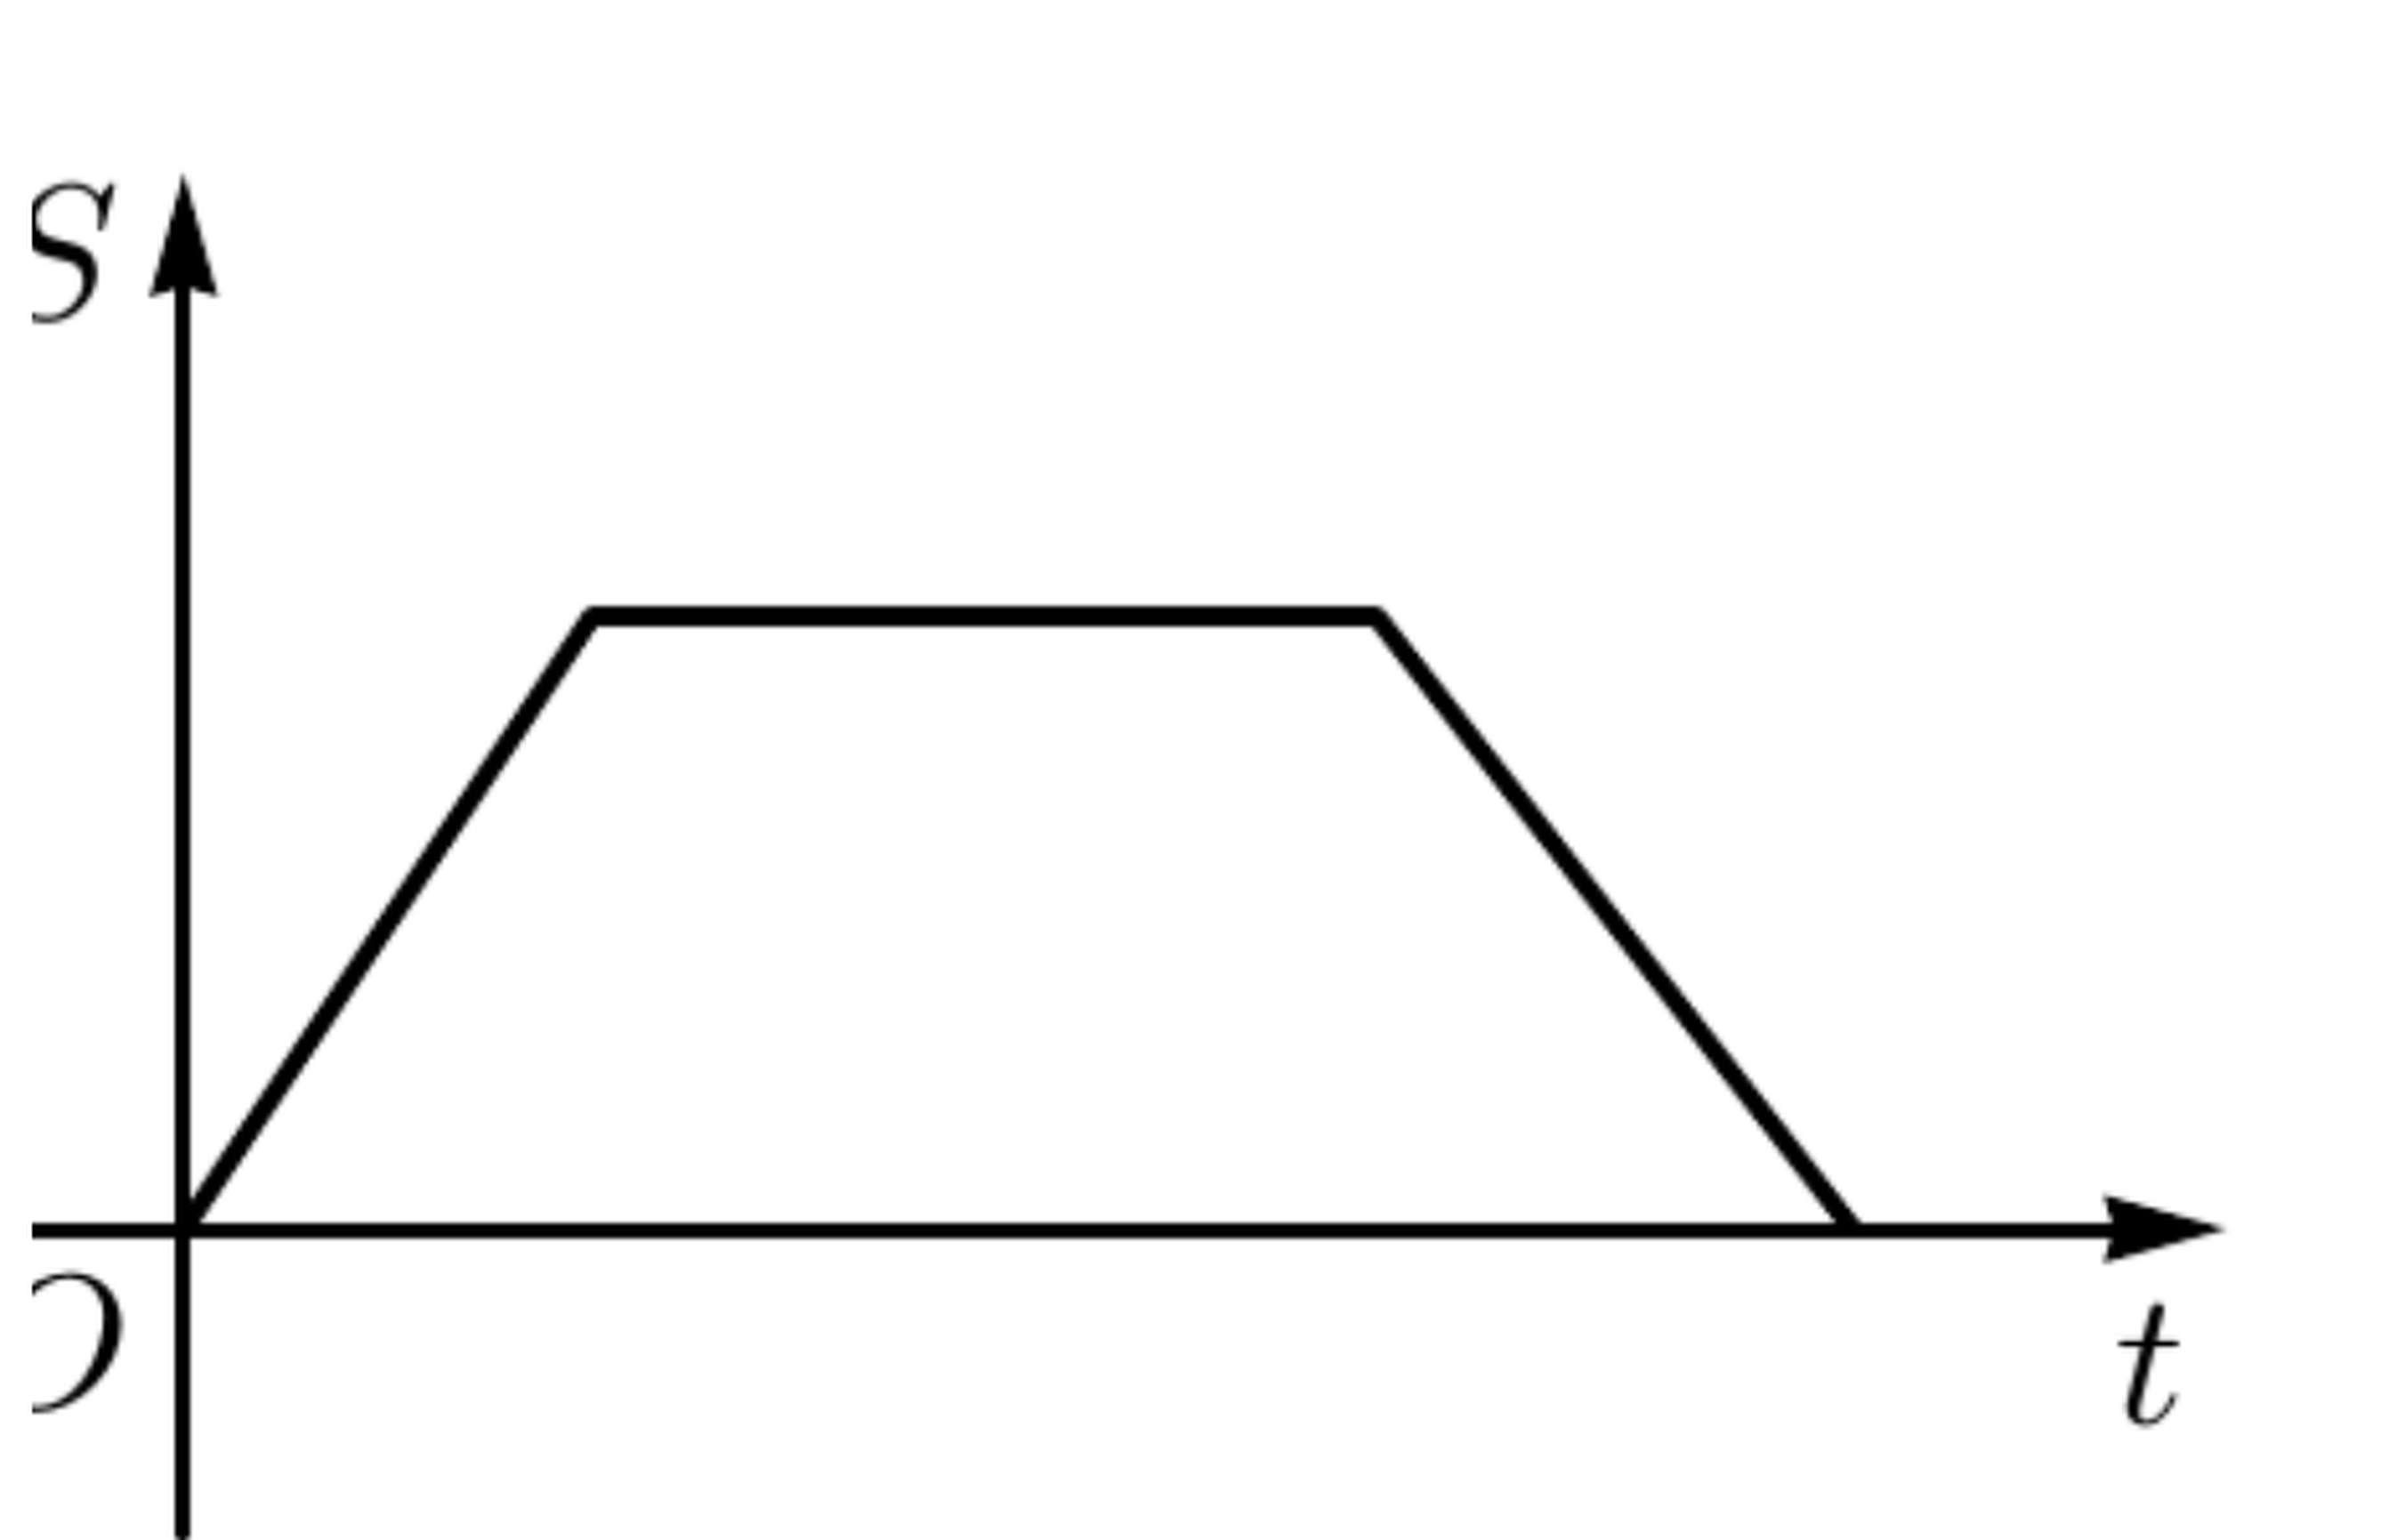
\includegraphics[width=0.34\textwidth]{figures/gao156_q14_st.png}
\end{center}

\keepwithprev
\begin{center}
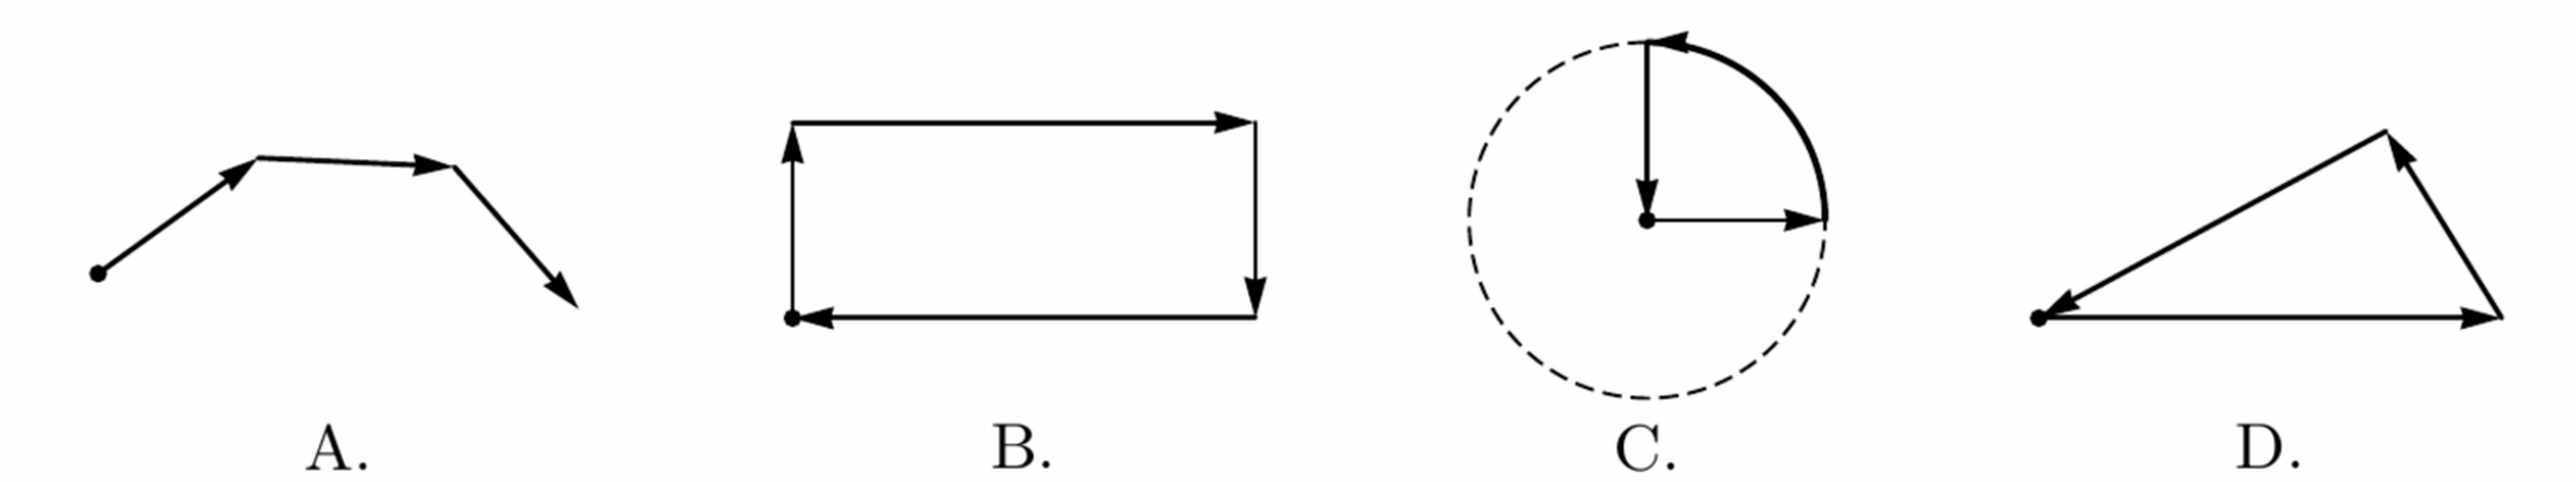
\includegraphics[width=0.86\textwidth]{figures/gao156_q14_opts.png}
\end{center}

\ifanswer
\solbegin
\step{由王老师锻炼时所走的离家距离（$S$）与行走时间（$t$）之间的函数关系图，}
\step{得在中间一段时间里，他到家的距离为定值，}
\step{故他所走的路程是一段以家为圆心的圆弧，故选 $C$.}
\solend
\fi

% === Q15 === 解析内曲线交点图（仅答案版出）；解析 4 行，故选 B
\item 已知 $a+2^a=b+\log_2 b=c+\log_3 c=k$，若 $k<1$，则\mbox{（\quad）}

\keepwithprev
A. $c<a<b$\qquad B. $a<c<b$\qquad C. $b<a<c$\qquad D. $a<b<c$

\ifanswer
\solbegin
\step{因为 $a+2^a=b+\log_2 b=c+\log_3 c=k$，}
\step{所以 $2^a=-a+k$，$\log_2 b=-b+k$，$\log_3 c=-c+k$，其中 $k<1$；}
\step{分别作出 $y=2^x$，$y=\log_2 x$，$y=\log_3 x$ 和 $y=-x+k$ 的图象，}

\begin{center}
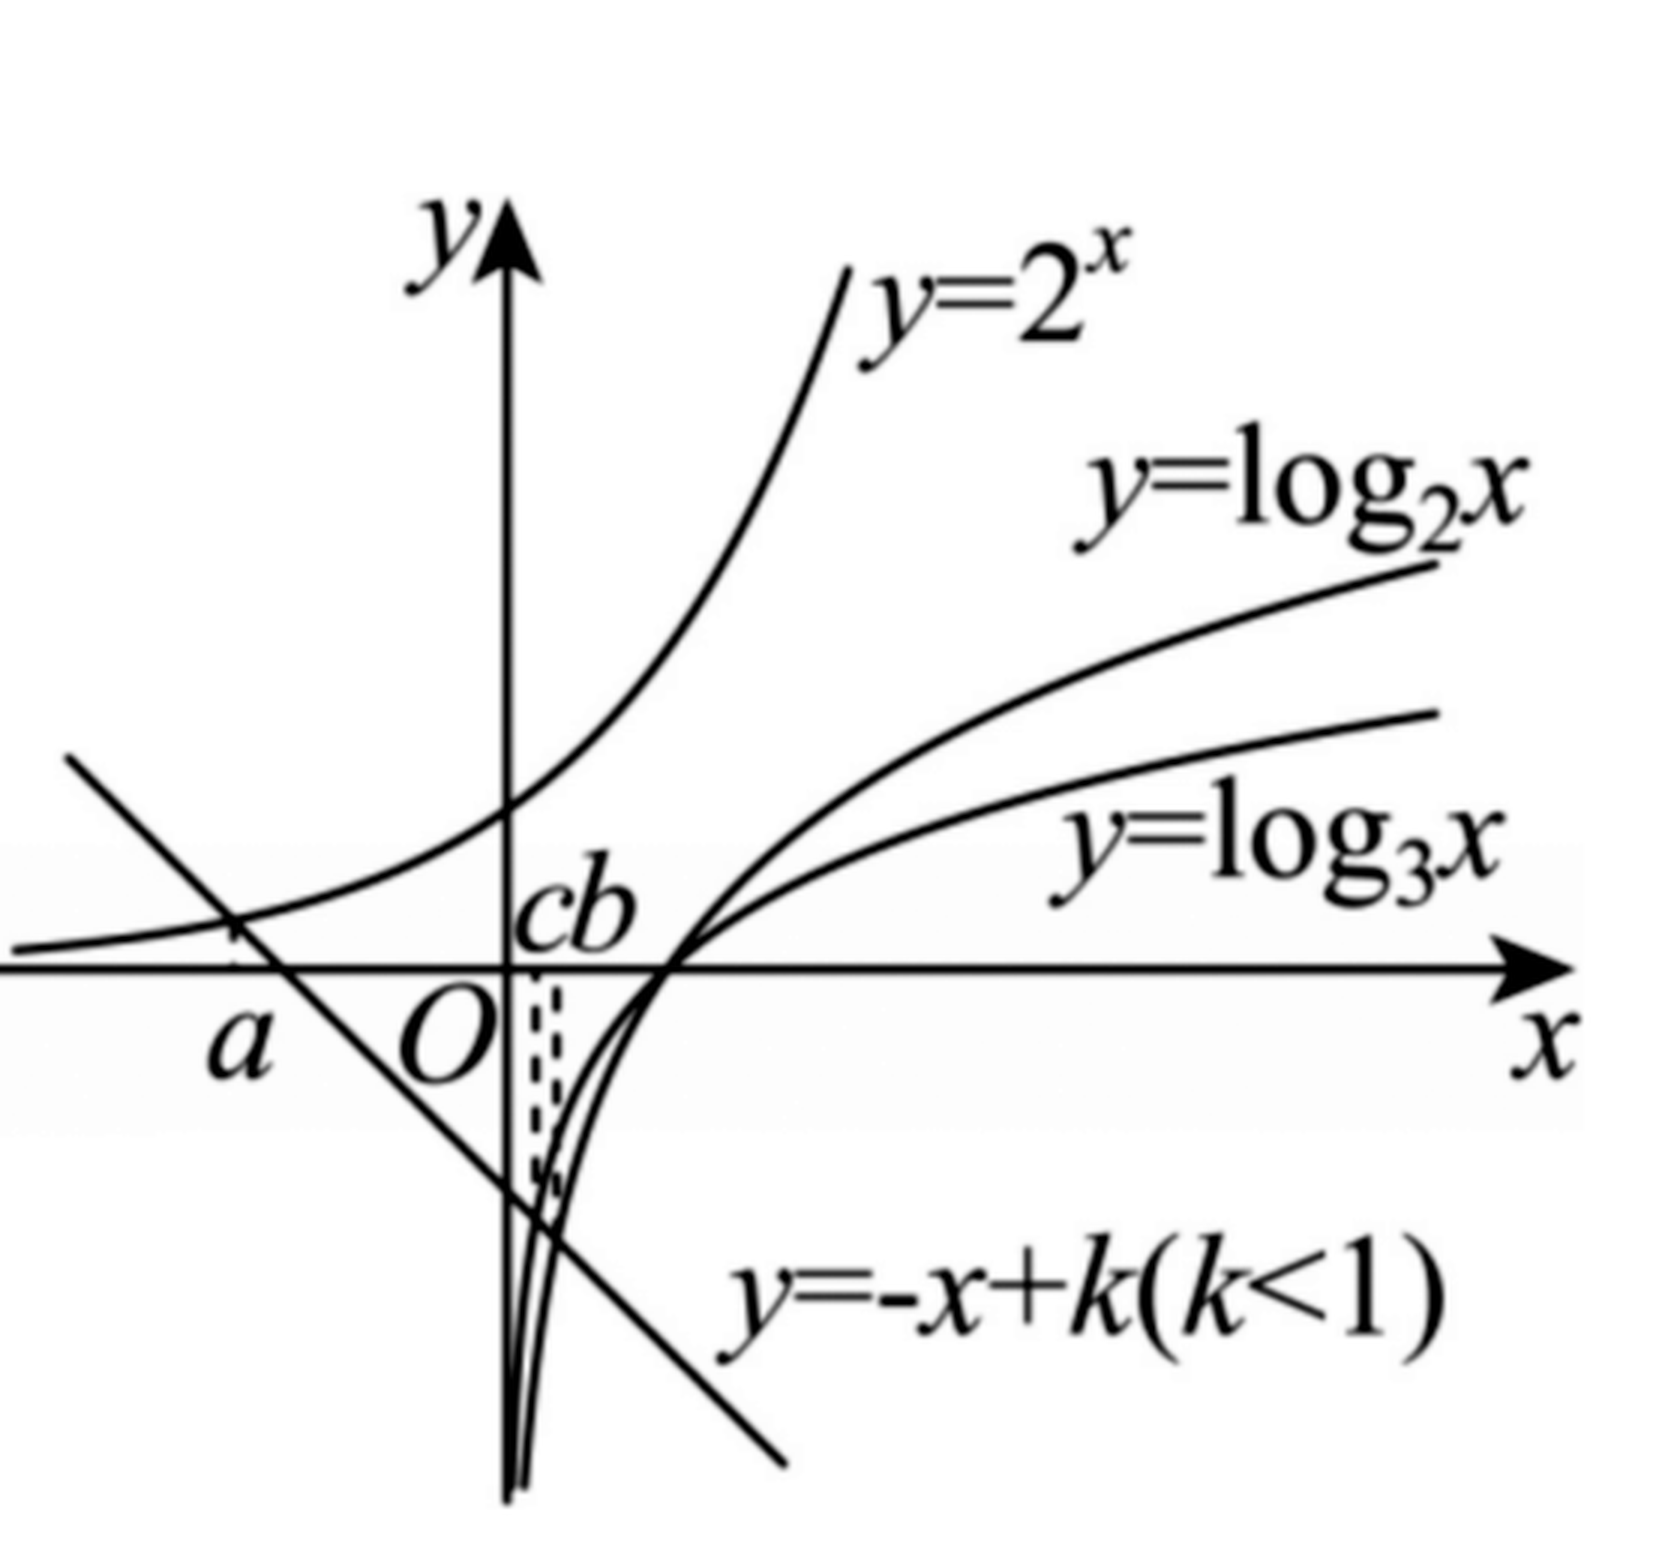
\includegraphics[width=0.52\textwidth]{figures/gao156_q15_curves.png}
\end{center}

\step{如图所示，由图象得 $a<c<b$. 故选 $B$.}
\solend
\fi

% === Q16 === ①② 文本圈数字、"一阶/二阶不动点""稳定点"自定义名词；解析 5 行，故选 A
\item 对定义域为 $I$ 的函数 $y=f(x)$，若存在 $x_0\in I$ 使得 $f(x_0)=x_0$，则称 $x_0$ 是函数 $f(x)$ 的
一阶不动点，简称不动点；若存在 $x_0\in I$ 使得 $f(f(x_0))=x_0$，则称 $x_0$ 是函数 $f(x)$ 的二阶
不动点，简称稳定点. 现有如下两个命题：①存在函数非 $y=x$ 且有无穷多个不动点；②
存在函数有无穷多个稳定点，且这些稳定点不都是不动点. 则\mbox{（\quad）}

\keepwithprev
A. ①成立，②成立\qquad\qquad B. ①成立，②不成立

C. ①不成立，②成立\qquad\qquad D. ①不成立，②不成立

\ifanswer
\solbegin
\step{①取定义在全体实数上的 $f(x)=\lvert x\rvert$，其不动点为一切非负实数，有无穷多个，}
\step{且 $f(-1)=1\ne-1$，①成立.}
\step{②取定义在全体实数上的 $g(x)=-x$，则 $g(g(x))=-(-x)=x$，}
\step{全体实数都是稳定点，而不动点只有 0，②成立.}
\step{故选 $A$.}
\solend
\fi

\end{enumerate}

\bigsec{三、解答题}

\begin{enumerate}
\setcounter{enumi}{16}

% === Q17 === $A\cap B$、$B\cap C$、\varnothing、\mid；解析 6 行
\item 设集合 $A=\{x\mid-1\leqslant x\leqslant2\}$，$B=\{x\mid2m<x<1\}$，$C=\{x\mid x<-1$ 或 $x>2\}$.

(1) 若 $A\cap B=B$，求实数 $m$ 的取值范围；

(2) 若 $B\cap C$ 中只有一个整数，求实数 $m$ 的取值范围.

\ifanswer
\solbegin
\step{(1) 当 $m\geqslant\dfrac12$ 时，$B=\varnothing$，满足 $A\cap B=B$.}
\step{当 $m<\dfrac12$ 时，$A\cap B=B$ 等价于 $2m\geqslant-1$，得 $-\dfrac12\leqslant m<\dfrac12$.}
\step{因此 $m$ 的取值范围为 $\left[-\dfrac12,+\infty\right)$.}
\step{(2) $B\cap C=\{x\mid2m<x<-1\}$，其中只有一个整数时，该整数必为 $-2$.}
\step{包含 $-2$ 且不包含 $-3$，等价于 $-3\leqslant2m<-2$，}
\step{因此 $m$ 的取值范围为 $\left[-\dfrac32,-1\right)$.}
\solend
\fi

% === Q18 === 幂函数 $x^{-\frac13}$、$m\in\R$；解析 12 行，跨 05—06 页
\item 已知幂函数 $f(x)=(3m^2-2m)x^m$（$m\in\R$）在定义域上不单调.

(1) 求函数 $f(x)$ 的解析式；

(2) 若 $f(a+1)<f(-2a+3)$，求实数 $a$ 的取值范围.

\ifanswer
\solbegin
\step{(1) 由幂函数的定义，$3m^2-2m=1$，即 $(3m+1)(m-1)=0$，得 $m=1$ 或 $m=-\dfrac13$.}
\step{当 $m=1$ 时，$f(x)=x$ 在定义域上单调递增，不合题意.}
\step{当 $m=-\dfrac13$ 时，$f(-1)=-1<f(1)=1$，而 $f(1)=1>f(8)=\dfrac12$，}
\step{故 $f(x)$ 在定义域上不单调.}
\step{因此 $f(x)=x^{-\frac13}$，定义域为 $(-\infty,0)\cup(0,+\infty)$.}
\step{(2) 有意义的条件为 $a\ne-1$ 且 $a\ne\dfrac32$.}
\step{当 $a<-1$ 时，$a+1<0<-2a+3$，有 $f(a+1)<0<f(-2a+3)$，}
\step{不等式成立.}
\step{当 $-1<a<\dfrac32$ 时，利用 $f(x)$ 在 $(0,+\infty)$ 上单调递减，}
\step{原不等式等价于 $a+1>-2a+3$，得 $\dfrac23<a<\dfrac32$.}
\step{当 $a>\dfrac32$ 时，$f(a+1)>0>f(-2a+3)$，不等式不成立.}
\step{所以 $a\in(-\infty,-1)\cup\left(\dfrac23,\dfrac32\right)$.}
\solend
\fi

% === Q19 === 两套解法（法一红字 \stepm，法二无标签）；\Delta 与 \subseteq；解析 21 行，跨 06—08 页
\item 已知 $a,c\in\R$，函数 $f(x)=\dfrac{x^2+(3a+1)x+c}{x+a}$.

(1) 若 $a=0$，求函数的定义域，并判断是否存在 $c$ 使得 $y=f(x)$ 图像关于原点对称，说明理由；

(2) 若函数过点 $(1,3)$，且函数 $y=f(x)$ 与 $x$ 轴负半轴有两个不同交点，求此时 $c$ 的值和 $a$ 的取值范围.

\ifanswer
\solbegin
\step{(1) 当 $a=0$ 时，$f(x)=\dfrac{x^2+(3a+1)x+c}{x+a}=\dfrac{x^2+x+c}{x}=x+\dfrac cx+1$，}
\step{故定义域为 $(-\infty,0)\cup(0,+\infty)$；}
\step{若存在实数 $c$，使得函数 $f(x)$ 为奇函数，则必有 $f(x)+f(-x)=0$，}
\step{而 $x+\dfrac cx+1+(-x)+\dfrac c{-x}+1=2\ne0$，}
\step{所以不存在实数 $c$，使得函数 $f(x)$ 为奇函数；}
\step{(2) 函数 $f(x)$ 的图像过点 $(1,3)$，则 $f(1)=\dfrac{1+(3a+1)+c}{1+a}=\dfrac{3a+c+2}{a+1}=3$，}
\step{解得 $c=1$，所以 $f(x)=\dfrac{x^2+(3a+1)x+1}{x+a}$，}
\stepm{法一：}{令 $f(x)=0$，则 $x^2+(3a+1)x+1=0$，此时方程有两不等负根，}
\step{则有 $\begin{cases}\Delta=(3a+1)^2-4>0\\-(3a+1)<0\end{cases}\Rightarrow\begin{cases}a>\dfrac13\text{ 或 }a<-1\\a>-\dfrac13\end{cases}\Rightarrow a>\dfrac13$，}
\step{注意到分母 $x+a\ne0$，则 $x\ne-a$，}
\step{若 $x=-a$ 也是方程 $x^2+(3a+1)x+1=0$ 的解，}
\step{代入方程 $(-a)^2+(3a+1)(-a)+1=0\Rightarrow2a^2+a-1=(a+1)(2a-1)=0$，}
\step{解得 $a=-1$ 或 $a=\dfrac12$，从而 $a\ne\dfrac12$，}
\step{综上，实数 $a$ 的取值范围为 $\left(\dfrac13,\dfrac12\right)\cup\left(\dfrac12,+\infty\right)$.}
\step{令 $g(x)=x^2+(3a+1)x+1$，与 $x$ 轴负半轴有两个交点，}
\step{则 $\begin{cases}-(3a+1)<0\\\Delta=(3a+1)^2-4>0\end{cases}\Rightarrow a>\dfrac13$.}
\step{注意到分母 $x+a\ne0$，则 $x\ne-a$，}
\step{若 $x=-a$ 也是方程 $x^2+(3a+1)x+1=0$ 的解，}
\step{代入方程 $(-a)^2+(3a+1)(-a)+1=0\Rightarrow2a^2+a-1=(a+1)(2a-1)=0$，}
\step{解得 $a=-1$ 或 $a=\dfrac12$，从而 $a\ne\dfrac12$，}
\step{综上，实数 $a$ 的取值范围为 $\left(\dfrac13,\dfrac12\right)\cup\left(\dfrac12,+\infty\right)$.}
\solend
\fi

% === Q20 === $Q$ 常数段 80000 照录；cases 与基本不等式；解析 10 行，跨 08—09 页
\item 某工厂生产某种零件的固定成本为 20000 元，每生产一个零件要增加投入 100 元，已知
总收入 $Q$（单位：元）关于产量 $x$（单位：个）满足函数：$Q=\begin{cases}400x-\dfrac12x^2,&0\leqslant x\leqslant400\\80000,&x>400\end{cases}$.

(1) 将利润 $P$（单位：元）表示为产量 $x$ 的函数；（总收入$=$总成本$+$利润）

(2) 当产量为何值时，零件的单位利润最大？最大单位利润是多少元？（单位利润$=$利润$\div$产量）

\ifanswer
\solbegin
\step{(1) 当 $0\leqslant x\leqslant400$ 时，}
\step{$P(x)=400x-\dfrac12x^2-20000-100x=-\dfrac12x^2+300x-20000$，}
\step{当 $x>400$ 时，$P(x)=80000-100x-20000=60000-100x$，}
\step{故 $P(x)=\begin{cases}-\dfrac12x^2+300x-20000,&0\leqslant x\leqslant400\\60000-100x,&x>400\end{cases}$.}
\step{(2) 设零件的单位利润为 $g(x)$，则 $g(x)=\begin{cases}-\dfrac12x-\dfrac{20000}{x}+300,&0\leqslant x\leqslant400\\\dfrac{60000}{x}-100,&x>400\end{cases}$，}
\step{当 $0\leqslant x\leqslant400$ 时，}
\step{$g(x)=300-\left(\dfrac12x+\dfrac{20000}{x}\right)\leqslant300-2\sqrt{\dfrac x2\cdot\dfrac{20000}{x}}=100$，}
\step{当且仅当 $\dfrac x2=\dfrac{20000}{x}$，即 $x=200$ 时取等号，}
\step{当 $x>400$ 时，$g(x)=\dfrac{60000}{x}-100$，此时无最值，}
\step{故当产量为 200 个，零件的单位利润最大，最大单位利润是 100 元.}
\solend
\fi

% === Q21 === 上升集定义、$D(x_0)=\{d\in\R\mid\cdots\}$、①②③ 文本圈数字、
%            \subseteq 带下划线、$-2^{-x}$；解析 19 行，跨 09—10 页
\item 已知函数 $y=f(x)$ 的定义域为 $\R$. 对任意 $x_0\in\R$，定义集合
$D(x_0)=\{d\in\R\mid f(x_0+d)>f(x_0)\}$，则称 $D(x_0)$ 为函数 $y=f(x)$ 在 $x_0$ 处的上升集.

(1) 若 $f(x)=1-x$，求 $D(-1)$；

(2) 若 $f(x)=\begin{cases}2^x,&x<0\\0,&x=0\\-2^{-x},&x>0\end{cases}$，求 $D(x)$；

(3) 设 $y=f(x)$ 满足：①当 $x<0$ 时，$f(x)=2^x$；②若 $f(x_1)\leqslant f(x_2)$，则
$D(x_2)\subseteq D(x_1)$；③当 $0<x<1$ 时，$f(x)<f(0)$. 证明：$f(0)\geqslant1$.

\ifanswer
\solbegin
\step{(1) $f(-1+d)>f(-1)\Leftrightarrow2-d>2\Leftrightarrow d<0$，所以 $D(-1)=(-\infty,0)$.}
\step{(2) 函数在 $(-\infty,0)$、$(0,+\infty)$ 上分别严格递增，}
\step{且这两个区间上的函数值分别为正、负，$f(0)=0$.}
\step{当 $x<0$ 时，$f(x+d)>f(x)\Leftrightarrow x<x+d<0\Leftrightarrow0<d<-x$，}
\step{当 $x=0$ 时，$f(d)>f(0)\Leftrightarrow d<0$，}
\step{当 $x>0$ 时，$f(x+d)>f(x)\Leftrightarrow x+d\leqslant0$ 或 $x+d>x$}
\step{$\Leftrightarrow d\leqslant-x$ 或 $d>0$，}
\step{因此 $D(x)=\begin{cases}(0,-x),&x<0\\(-\infty,0),&x=0\\(-\infty,-x]\cup(0,+\infty),&x>0\end{cases}$.}
\step{(3) 任取 $a\in(-1,0)$，}
\step{令 $d=-\dfrac a2$，则 $0<d<1$，且 $f(a+d)=2^{\frac a2}>2^a=f(a)$，}
\step{所以 $d\in D(a)$；}
\step{由③，$f(d)<f(0)$，所以 $d\notin D(0)$.}
\step{若 $f(0)\leqslant f(a)$，由②得 $D(a)\subseteq D(0)$，与上述结论矛盾.}
\step{因此，对任意 $a\in(-1,0)$，都有 $f(0)>2^a$.}
\step{特别地 $f(0)>2^{-\frac12}>0$.}
\step{若 $f(0)<1$，取 $a=\dfrac12\log_2 f(0)$，则 $-\dfrac14<a<0$，且}
\step{$2^a=\sqrt{f(0)}>f(0)$，}
\step{与 $f(0)>2^a$ 矛盾.}
\step{所以 $f(0)\geqslant1$.}
\solend
\fi

\end{enumerate}

\end{document}
"
% 紧凑版：xelatex "\def\iscompact{1}% 高一156_大同中学_期中.tex
%   —— 高一上数学"2026-2027 年大同中学高一上期中"（试卷版/答案版/紧凑版）
% 试卷版：xelatex 高一156_大同中学_期中.tex
% 答案版：xelatex "\def\isanswer{1}\input{高一156_大同中学_期中.tex}"
% 紧凑版：xelatex "\def\iscompact{1}\input{高一156_大同中学_期中.tex}"
%
% ① 原始材料：微信公众号"魔都数学加油站"文章，连载"27学年高一156"，原文标题
% "27学年高一156——2026-2027年上海市大同中学高一上期中"；
% 原文链接：https://mp.weixin.qq.com/s/xLtS5tyjCPJIWCIBohwGvw 。
% 正文为 10 张 PNG 页（01/02/03/04/05/06/07/08/09/10 各页分辨率混排
% 2560×3620 与 4762×6735，逐页按各自分辨率裁图核对）。
% 体例：讲评版——填空 3—12（10 题）、选择 13—16（4 题）、解答 17—21（5 题），
% 共 19 题，自第 3 题起编（1、2 未印在本篇）；Q3 只印【答案】、其余 18 题
% 逐题印【解析】（逐题核实，见 ②）。题目、答案、解析均据原图转录；卷面粉红色
% 水印"魔都数学加油站"及公众号页脚未录入。
%
% 卷首标题：原卷印作"2026-2027 年大同中学高一上期中"，年份区间按全稿惯例排 en dash；
% 原卷卷面未印副标题，本稿按同期中卷知识模块口径补出"集合与常用逻辑用语、不等式、函数"。
%
% ② 与原卷的排版差异：
%   ① 原文从第 3 题起，本稿保留原题号；共 19 题三节，解答题 5 题到 21；
%   ② 混合体例：第 3 题只印【答案】、无【解析】，按 高一140 第 5 题／高一145
%      第 3 题／高一151 第 7 题成例另提 \ans{}、不补造解析；其余 18 题印
%      【解析】、用 \solbegin…\solend；四道选择题答案在解析末句"故选 C／C／B／A"
%      （逐个放大复核）、括号 \mbox{（\quad）} 留空、不另提 \ans{}；答案版
%      【答案】/【解析】标记数 = 19 = 全卷题数（1 个 \ans ＋ 18 个 \solbegin）；
%   ③ 原卷卷面未印副标题，本稿按知识模块口径补出；
%   ④ 原卷填空横线按全稿惯例排 \blankline[4.4em]；选择题括号排 \mbox{（\quad）}、
%      选项段前按惯例各加 \keepwithprev；解答题不留作答区、不加 \anspace
%      （原卷为讲评版，109—113 起全稿不用 \anspace）；
%   ⑤ 数集：Q3"$x\in\R$"、Q18"$m\in\R$"、Q19"$a,c\in\R$"、Q21"定义域为 \R"
%      "任意 $x_0\in\R$""$d\in\R$"原卷印正体粗体 R，按全稿惯例归一 \R；
%      绝对值排 \lvert…\rvert（Q11 $\lvert2^x-1\rvert$、Q16 $\lvert x\rvert$），
%      集合描述竖线排 \mid（Q17 $A=\{x\mid\cdots\}$、Q21 $D(x_0)=\{d\in\R\mid\cdots\}$），
%      空集 \varnothing（Q17"$B=\varnothing$"），不等号按全稿惯例排 \leqslant／\geqslant；
%   ⑥ 子集符号逐处照录不统一：Q21 (3) 题干"$D(x_2)\subseteq D(x_1)$"与解析
%      "$D(a)\subseteq D(0)$"均印带下划线 ⊆，照录 \subseteq；本卷无单线 ⊂ 用例；
%   ⑦ 判别式：Q19 两套解法"$\Delta=(3a+1)^2-4>0$"印等腰偏高 \Delta，照录 \Delta；
%      本卷无扁三角 \triangle 用例；
%   ⑧ 红字照录为黑体：Q19 (2) 解析第一套解法行首"法一："原卷排**红色加粗**，
%      按 高一53 成例排 \stepm{法一：}{…}（加粗着色、不改黑色基调），全库无红字
%      排字先例、本稿不引入红色定义，文件头注明；第二套解法原卷直接以
%      "令 $g(x)=x^2+(3a+1)x+1$，与 $x$ 轴负半轴有两个交点，"另起，
%      **未印"法二："标签**（逐页像素级复核：07 页仅 1437—1475 一处红字，
%      08 页无红字），照录为普通 \step、不补造标签；
%   ⑨ 文本模式圈数字逐处照录：Q12 解析 ①② 两情形、Q16 两则命题与四个选项及
%      解析的 ①②、Q21 (3) 三条件 ①②③ 与解析"由③""由②"，均为印刷圈数字
%      （非 \textcircled、非数学模式），计入圈数字实测；
%   ⑩ 自定义名词照录：Q16"一阶不动点，简称不动点""二阶不动点，简称稳定点"、
%      Q21"上升集"；Q16 题干"存在函数非 $y=x$ 且有无穷多个不动点"照录；
%   ⑪ 中文弯引号照录：Q3""存在 $x\in\R$，$x^3-1\leqslant0$" 否定形式为"、
%      Q13"使"$\dfrac{x+1}{1-x}\geqslant0$"成立的必要不充分条件是"；
%      注释里一律 ASCII 引号；数学式内 CJK 用 \text{}（Q19 cases 内"或"）；
%   ⑫ 半角逗号在数学组之间是全稿惯例、非笔误，逐处照录（$a,c$、$x,y$、$a,b$
%      之类）；行末西文句点 ASCII `.`；行中全角逗号／顿号照录；
%   ⑬ 复杂式照录别简化：Q6 $\left(\dfrac{1}{\sqrt a}\right)^{\frac27}\cdot\sqrt[7]{a^3}$
%      与解析 $a^{\frac{12}{7}-\frac17+\frac37}$、Q8 $2\sqrt4+5=9$（$\sqrt4$ 未化简）、
%      Q9 $\left(\sqrt x+\dfrac{1}{\sqrt x}\right)^3$、Q12 $\dfrac{4a-(2-a)^2}{4a}$、
%      Q18 $f(8)=\dfrac12$、Q19 $2a^2+a-1=(a+1)(2a-1)=0$、Q20 $Q$ 的常数段
%      $80000$（不是 $80000-100x$）与 $2\sqrt{\dfrac x2\cdot\dfrac{20000}{x}}$、
%      Q21 $f(a+d)=2^{\frac a2}>2^a=f(a)$ 与 $2^a=\sqrt{f(0)}>f(0)$ 等；
%      \left…\right 不得拆到不同 $…$ 组（Q5 $\left(0,\dfrac12\right)$、
%      Q12 $\left[0,4+2\sqrt3\right)$、Q17 $\left[-\dfrac12,+\infty\right)$、
%      Q19 $\left(\dfrac13,\dfrac12\right)\cup\left(\dfrac12,+\infty\right)$、
%      Q20 $\left(\dfrac12x+\dfrac{20000}{x}\right)$ 等）；cases 块整体算一个印刷行；
%   ⑭ 一条 \step = 原卷解析的一个印刷行；别并折行、别拆行。跨页续印按题合并
%      （Q6 的 01 页上下题干重复印、Q8 的 01—02 页、Q12 的 02—03 页、
%      Q15 的 04 页上下、Q16 的 04—05 页、Q17 的 05 页上下、Q18 的 05—06 页、
%      Q19 的 06—08 页、Q20 的 08—09 页、Q21 的 09—10 页）；
%      跨半页重叠行（Q12 的"②若 …"、Q18 的"原不等式等价于 …"、
%      Q20 的"【解析】(1) 当 $0\leqslant x\leqslant400$ 时，"、Q21 的
%      "【解析】(1) $f(-1+d)>f(-1)\cdots$"与"与 $f(0)>2^a$ 矛盾."）
%      只算一个印刷行；
%   ⑮ 配图：全卷 3 组（逐页通读 10 页确认）——
%      · Q14 题干 S-t 梯形图（03 页右下，离家距离 S 对行走时间 t），题目配图、
%        三版都出，裁 figures/gao156_q14_st.png；
%      · Q14 四幅路线选项（04 页上部，A/B/C/D 四幅横排、C 为以家为圆心的圆弧），
%        题目配图、三版都出，合并成一张，裁 figures/gao156_q14_opts.png；
%      · Q15 解析内曲线交点图（04 页右下，$y=2^x$、$y=\log_2x$、$y=\log_3x$
%        与 $y=-x+k$），仅答案版出，裁 figures/gao156_q15_curves.png；
%      3 图均取自原卷截图，去粉色水印、去色、3×~4× LANCZOS 放大；
%      Q14 题干"题干＋两图"整块用 \needvspace 守卫推走（守卫放 \item 之前，
%      见 高一154 Q15／高一136 Q13 成例）；Q15 解析内图放 \ifanswer 内
%      \solbegin…\solend 的两 \step 之间（高一108 第 6 题／高一154 附加题 2 成例）；
%      其余各页逐页确认无其它题目配图、无解析配图、无表格；10 页下半仅水印、无正文。
%
% ③ 行数复核：一条 \step = 原卷解析的一个印刷行，cases 块作一个印刷行计。
%   逐题数（主会话逐页核对定稿）：Q3：0（只印【答案】、提 \ans{}，不计入 \step 账）；
%   Q4：1；Q5：1；Q6：1；Q7：1；Q8：3；Q9：2；Q10：2；Q11：5；Q12：12；
%   Q13：3；Q14：3；Q15：4；Q16：5；Q17：6；Q18：12；Q19：21；Q20：10；Q21：19。
%   合计 111 行（110 条 \step ＋ 1 条 \stepm），与原卷逐题印刷行相等。
%   全卷 19 题：Q3 一处 \ans{} ＋ 其余 18 题设 \solbegin…\solend，
%   答案版【答案】/【解析】标记数 = 19 = 全卷题数。
%
% ④ 页码分布（供回原图复核）：
%   卷首标题＋"一、填空题"＋Q3 题干＋【答案】、Q4 题干＋解析 1 行、
%   Q5 题干＋解析 1 行、Q6 题干首行在 01 页上半；
%   Q6 题干（重复印）＋解析 1 行、Q7 题干＋解析 1 行、Q8 题干＋解析前 2 行
%   在 01 页下半；Q8 解析末行、Q9 题干＋解析 2 行、Q10 题干＋解析 2 行、
%   Q11 题干首行在 02 页上半；Q11 题干（重复印）＋解析 5 行、
%   Q12 题干＋解析首行在 02 页下半；Q12 解析中 9 行在 03 页上半；
%   Q12 解析末 2 行＋"二、选择题"标题＋Q13 题干＋选项＋解析 3 行＋
%   Q14 题干首行在 03 页下半；Q14 题干续行＋四幅选项图＋解析 3 行＋
%   Q15 题干＋选项＋解析前 2 行＋Q16 题干在 04 页上半；
%   Q15 解析后 2 行＋曲线图＋Q16 选项＋解析前 2 行在 04 页下半；
%   Q16 解析后 3 行＋"三、解答题"标题＋Q17 题干＋两问＋解析 (1) 3 行
%   在 05 页上半；Q17 解析 (2) 3 行＋Q18 题干＋两问＋解析 (1) 首 2 行
%   在 05 页下半；Q18 解析 (1)(2) 中 8 行在 06 页上半；Q18 解析末 2 行＋
%   Q19 题干＋两问＋解析 (1) 首行在 06 页下半；Q19 解析 (1) 后 4 行＋
%   (2) 前 2 行＋法一 2 行在 07 页上半；法一后 5 行＋法二前 3 行在 07 页下半；
%   法二后 4 行＋Q20 题干＋两问＋解析 (1) 首行在 08 页上半；
%   Q20 解析 (1) 后 3 行＋(2) 前 5 行在 08 页下半；Q20 解析 (2) 末 2 行＋
%   Q21 题干＋三问＋解析 (1) 首行在 09 页上半；Q21 解析 (1)（重复印）＋
%   (2) 8 行＋(3) 首行在 09 页下半；Q21 (3) 解析中 8 行在 10 页上半；
%   Q21 (3) 末 2 行在 10 页下半。本稿按题连排，不丢行、不并折行；
%   全卷末题为第 21 题，无附加题节。
%
\documentclass[a4paper,11pt]{article}
\usepackage{common}

\begin{document}

\examtitlest[3]{2026--2027 年大同中学高一上期中}{集合与常用逻辑用语、不等式、函数}

\bigsec{一、填空题}

\begin{enumerate}
\setcounter{enumi}{2}

% === Q3 === 只印【答案】、无【解析】；R 正体粗体 \R；中文弯引号照录
\item “存在 $x\in\R$，$x^3-1\leqslant0$” 否定形式为\blankline[4.4em].

\ifanswer
\ans{对任意 $x\in\R$，$x^3-1>0$}
\fi

% === Q4 === 解析 1 行
\item 若实数 $a>0$ 且 $a\ne1$，函数 $y=a^{x-3}+1$ 的图像恒过定点 $P$，则点 $P$ 的坐标为\blankline[4.4em].

\ifanswer
\solbegin
\step{当 $x=3$ 时，$y=a^0+1=2$，与 $a$ 无关，所以定点为 $P(3,2)$.}
\solend
\fi

% === Q5 === 解析 1 行
\item 函数 $y=\dfrac{1}{3^x+2}$ 的值域是\blankline[4.4em].

\ifanswer
\solbegin
\step{$3^x\in(0,+\infty)$，因此 $3^x+2\in(2,+\infty)$，值域为 $\left(0,\dfrac12\right)$.}
\solend
\fi

% === Q6 === 根式嵌套照录；解析 1 行；题干跨 01 页上下重复印
\item 已知 $a>0$，化简 $a^{\frac{12}{7}}\cdot\left(\dfrac{1}{\sqrt a}\right)^{\frac27}\cdot\sqrt[7]{a^3}=$\blankline[4.4em].

\ifanswer
\solbegin
\step{原式 $=a^{\frac{12}{7}}\cdot a^{-\frac17}\cdot a^{\frac37}=a^{\frac{12}{7}-\frac17+\frac37}=a^2$.}
\solend
\fi

% === Q7 === 换底公式；解析 1 行
\item 已知 $\log_5 3=a$，用 $a$ 的代数式表示 $\log_{15}125=$\blankline[4.4em].

\ifanswer
\solbegin
\step{$\log_{15}125=\dfrac{\log_5 125}{\log_5 15}=\dfrac{3}{1+\log_5 3}=\dfrac{3}{1+a}$.}
\solend
\fi

% === Q8 === 基本不等式，$\sqrt4$ 照录未化简；解析 3 行，跨 01—02 页
\item 已知 $x>0$，$y>0$，且 $4x+y=xy$，则 $x+y$ 的最小值为\blankline[4.4em].

\ifanswer
\solbegin
\step{由 $4x+y=xy$，得 $\dfrac4y+\dfrac1x=1$，}
\step{则 $x+y=(x+y)\left(\dfrac4y+\dfrac1x\right)=\dfrac{4x}{y}+\dfrac yx+1+4\geqslant2\sqrt4+5=9$，}
\step{当且仅当 $\dfrac{4x}{y}=\dfrac yx$，即 $x=3$，$y=6$ 时取等号，故最小值为 9.}
\solend
\fi

% === Q9 === 解析 2 行
\item 已知 $x^{-1}+x=7$（$x>0$），则 $x^{\frac32}+x^{-\frac32}$ 的值为\blankline[4.4em].

\ifanswer
\solbegin
\step{$x>0$，有 $\sqrt x+\dfrac{1}{\sqrt x}=\sqrt{x+\dfrac1x+2}=3$，}
\step{所以 $x^{\frac32}+x^{-\frac32}=\left(\sqrt x+\dfrac{1}{\sqrt x}\right)^3-3\left(\sqrt x+\dfrac{1}{\sqrt x}\right)=27-9=18$.}
\solend
\fi

% === Q10 === $x_{\min}$；解析 2 行
\item 已知不等式 $x>\dfrac{2a+1}{a-1}$ 对任意的 $x\in[1,2]$ 恒成立，则实数 $a$ 的取值范围是\blankline[4.4em].

\ifanswer
\solbegin
\step{不等式 $x>\dfrac{2a+1}{a-1}$ 对任意的 $x\in[1,2]$ 恒成立，得 $\dfrac{2a+1}{a-1}<x_{\min}=1$，}
\step{即有 $\dfrac{a+2}{a-1}<0$，解得 $-2<a<1$，则实数 $a$ 的取值范围是 $(-2,1)$.}
\solend
\fi

% === Q11 === 分段函数 cases 与绝对值 \lvert…\rvert；解析 5 行
\item 已知函数 $f(x)=\begin{cases}\lvert2^x-1\rvert-a,&x\leqslant2\\\dfrac{3}{x-1}-a,&x>2\end{cases}$，若函数 $y=f(x)$ 图像与 $x$ 轴有三个不同交点，则实数 $a$ 的取值范围是\blankline[4.4em].

\ifanswer
\solbegin
\step{令 $g(x)=f(x)+a$.}
\step{在 $(-\infty,0)$、$[0,2]$、$(2,+\infty)$ 上，$g(x)$ 均严格单调，}
\step{值域依次为 $(0,1)$、$[0,3]$、$(0,3)$.}
\step{每段至多有一个交点，因而恰有三个不同交点，}
\step{当且仅当 $a\in(0,1)\cap[0,3]\cap(0,3)=(0,1)$.}
\solend
\fi

% === Q12 === ①② 文本圈数字、对称轴与最小值式照录；解析 12 行，跨 02—03 页
\item 已知函数 $f(x)=ax^2-(2-a)x+1$，$g(x)=x$，若对于任意实数 $x$，$f(x)$ 与 $g(x)$ 至少有一个为正数，则实数 $a$ 的取值范围是\blankline[4.4em].

\ifanswer
\solbegin
\step{当 $x>0$ 时，$g(x)>0$；当 $x<0$ 时，$g(x)<0$；}
\step{当 $x=0$ 时，$f(0)=1>0$；}
\step{因为对于任意实数 $x$，$f(x)$ 与 $g(x)$ 至少有一个为正数，}
\step{当 $x<0$ 时，因为 $g(x)<0$，所以 $f(x)=ax^2-(2-a)x+1>0$ 恒成立，}
\step{当 $a<0$ 时，显然不成立，}
\step{当 $a=0$ 时，$f(x)=-2x+1>0$，对 $x<0$ 时恒成立，满足题意，}
\step{当 $a>0$ 时，函数图象开口向上，对称轴 $x=\dfrac{2-a}{2a}$，}
\step{①若 $\dfrac{2-a}{2a}\geqslant0$，即 $0<a\leqslant2$ 时，函数 $f(x)$ 在 $(-\infty,0)$ 上严格减，$f(0)=1$，}
\step{故 $f(x)>0$ 对 $x<0$ 时恒成立，满足题意；}
\step{②若 $\dfrac{2-a}{2a}<0$，即 $a>2$ 时，$f(x)_{\min}=f\left(\dfrac{2-a}{2a}\right)=\dfrac{4a-(2-a)^2}{4a}>0$，}
\step{解得 $4-2\sqrt3<a<4+2\sqrt3$，所以 $2<a<4+2\sqrt3$.}
\step{综上，$0\leqslant a<4+2\sqrt3$，故实数 $a$ 的取值范围是 $\left[0,4+2\sqrt3\right)$.}
\solend
\fi

\end{enumerate}

\bigsec{二、选择题}

\begin{enumerate}
\setcounter{enumi}{12}

% === Q13 === 必要不充分条件；cases 块；解析 3 行，故选 C
\item 使 “$\dfrac{x+1}{1-x}\geqslant0$” 成立的必要不充分条件是\mbox{（\quad）}

\keepwithprev
A. $-1\leqslant x<1$\qquad B. $x\leqslant-1$ 或 $x>1$\qquad C. $-1\leqslant x\leqslant1$\qquad D. $x\leqslant-1$ 或 $x\geqslant0$

\ifanswer
\solbegin
\step{由不等式 $\dfrac{x+1}{1-x}\geqslant0$ 得 $\begin{cases}(x+1)(1-x)\geqslant0\\1-x\ne0\end{cases}$，解得 $-1\leqslant x<1$，}
\step{由题意结合选项，$-1\leqslant x<1\Rightarrow-1\leqslant x\leqslant1$ 成立，反之不成立，}
\step{所以 $-1\leqslant x\leqslant1$ 是 $\dfrac{x+1}{1-x}\geqslant0$ 成立的必要不充分条件. 故选 $C$.}
\solend
\fi

% === Q14 === 题干 S-t 图＋四幅路线选项（题目配图，三版都出）；守卫放 \item 之前；解析 3 行，故选 C
\needvspace{9cm}
\item 如图是王老师锻炼时所走的离家距离（$S$）与行走时间（$t$）之间的函数关系图，若
用黑点表示王老师家的位置，则王老师行走的路线可能是\mbox{（\quad）}

\begin{center}
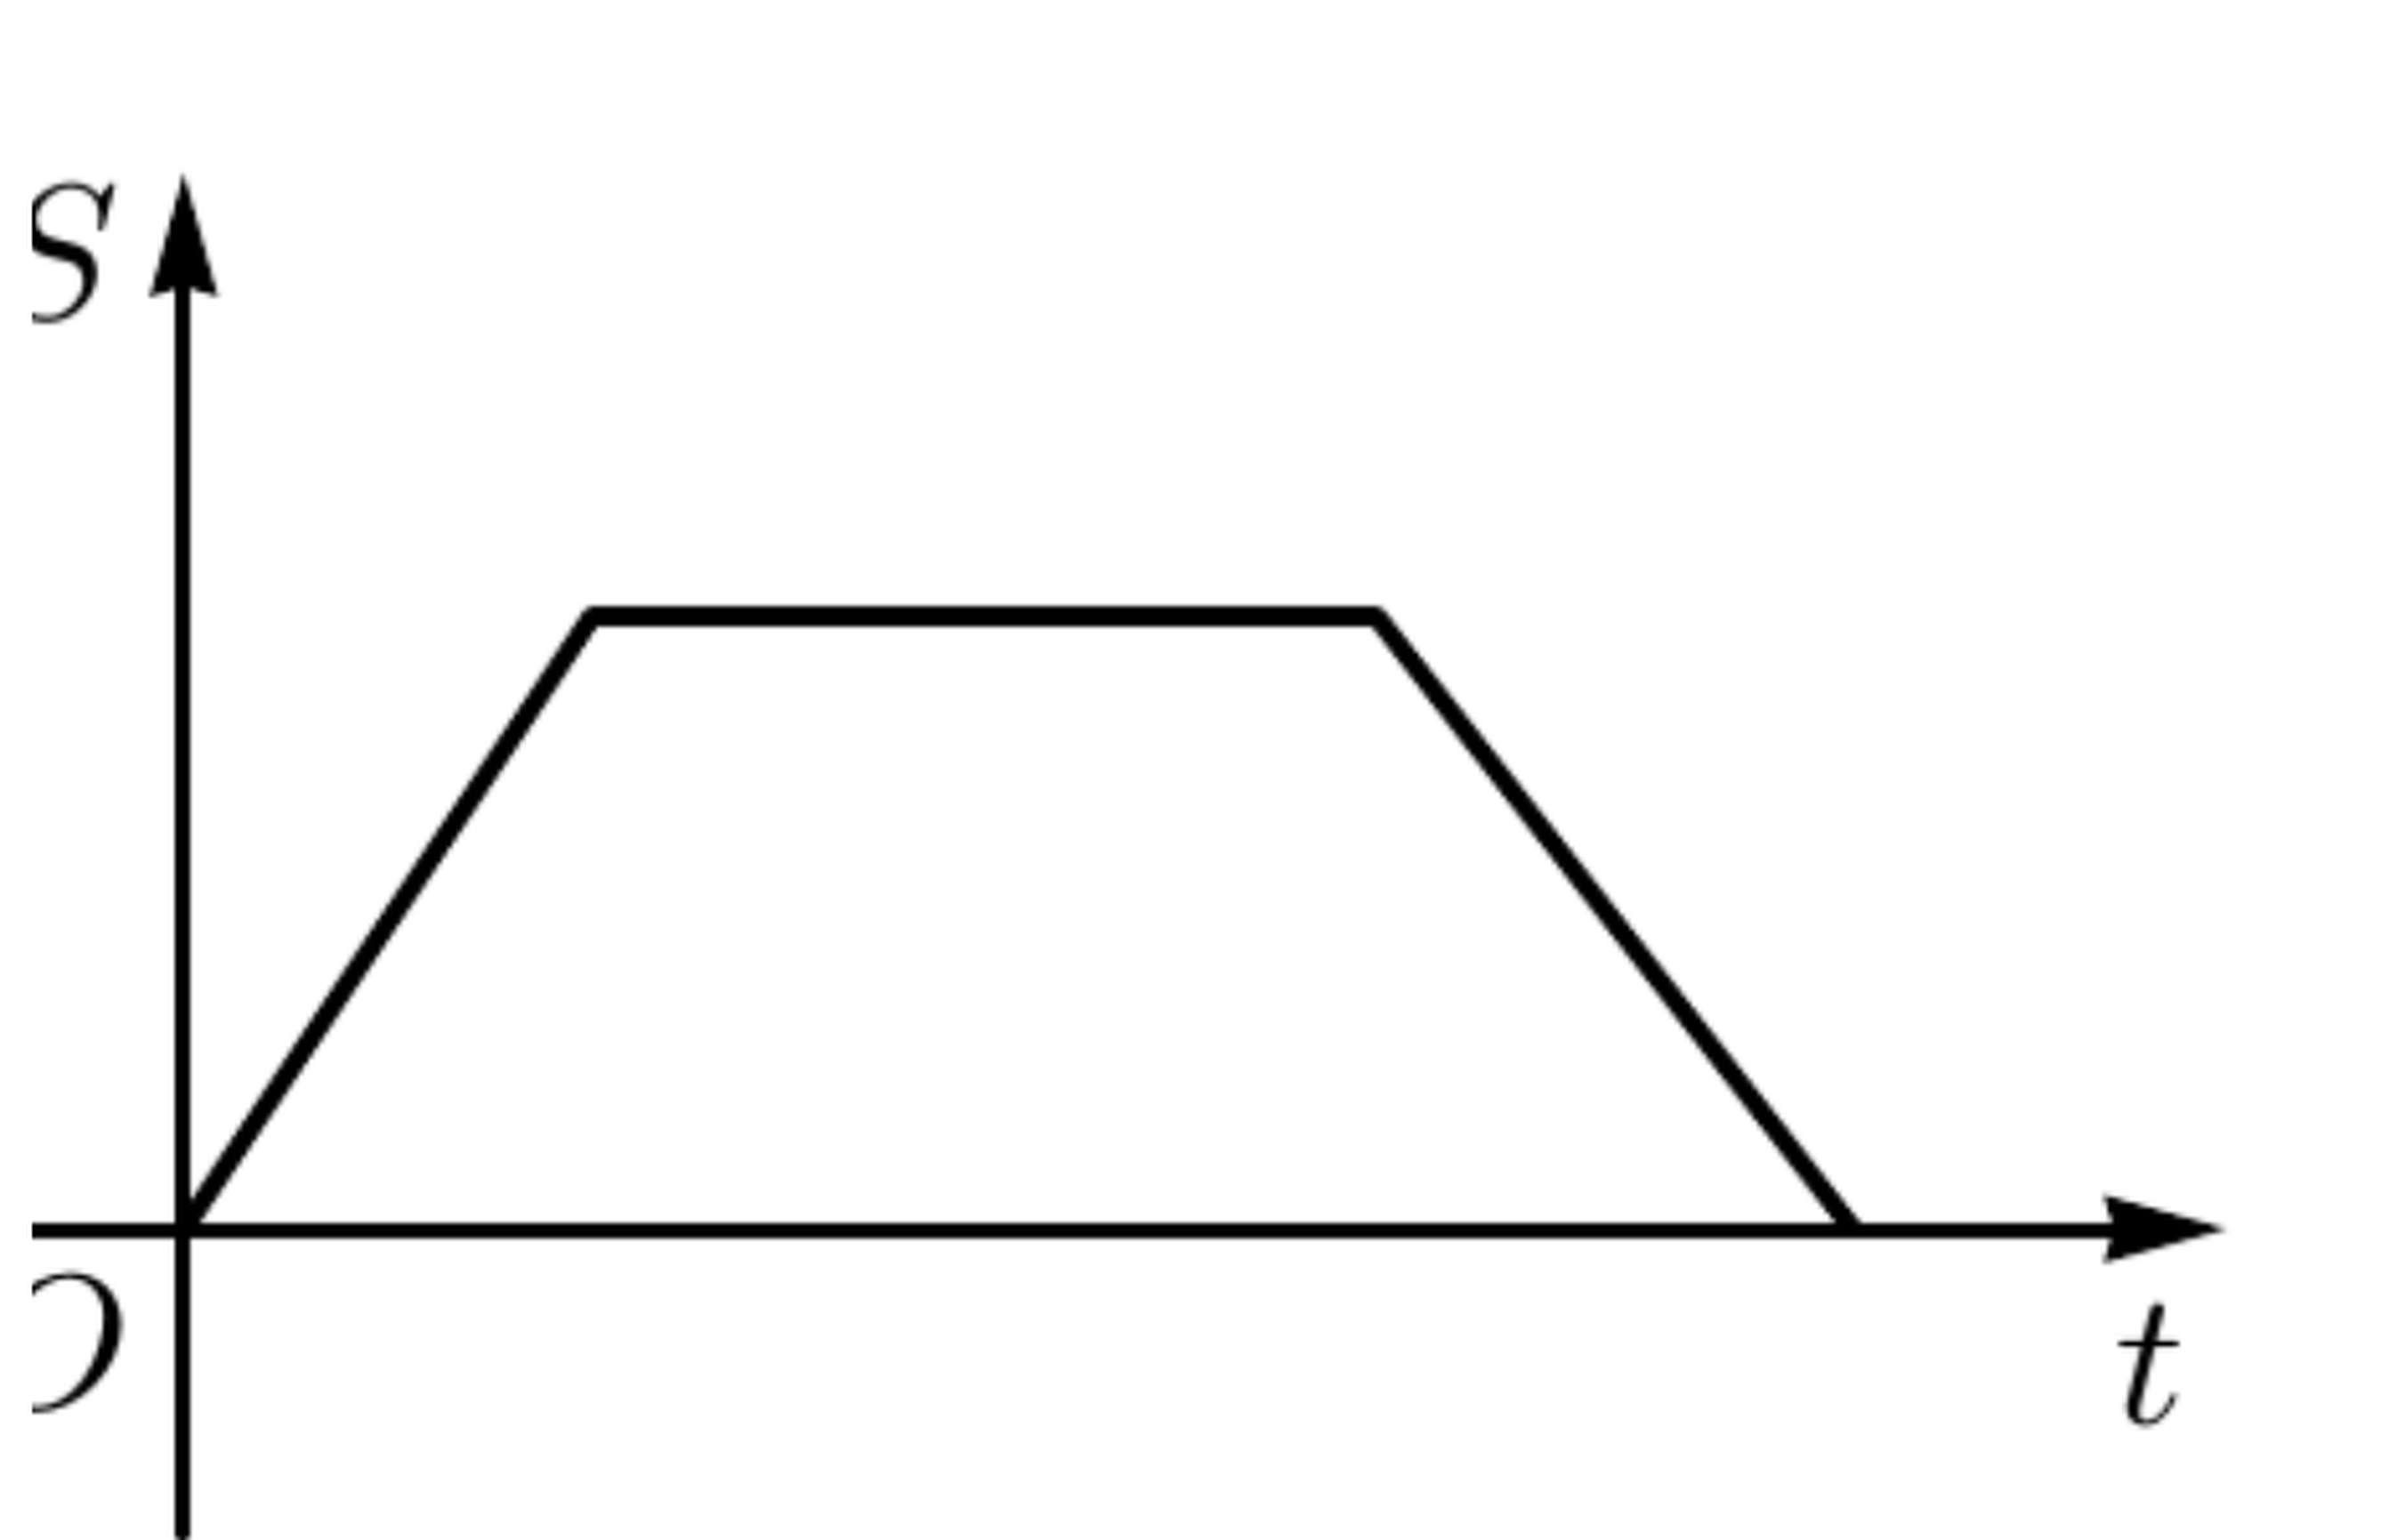
\includegraphics[width=0.34\textwidth]{figures/gao156_q14_st.png}
\end{center}

\keepwithprev
\begin{center}
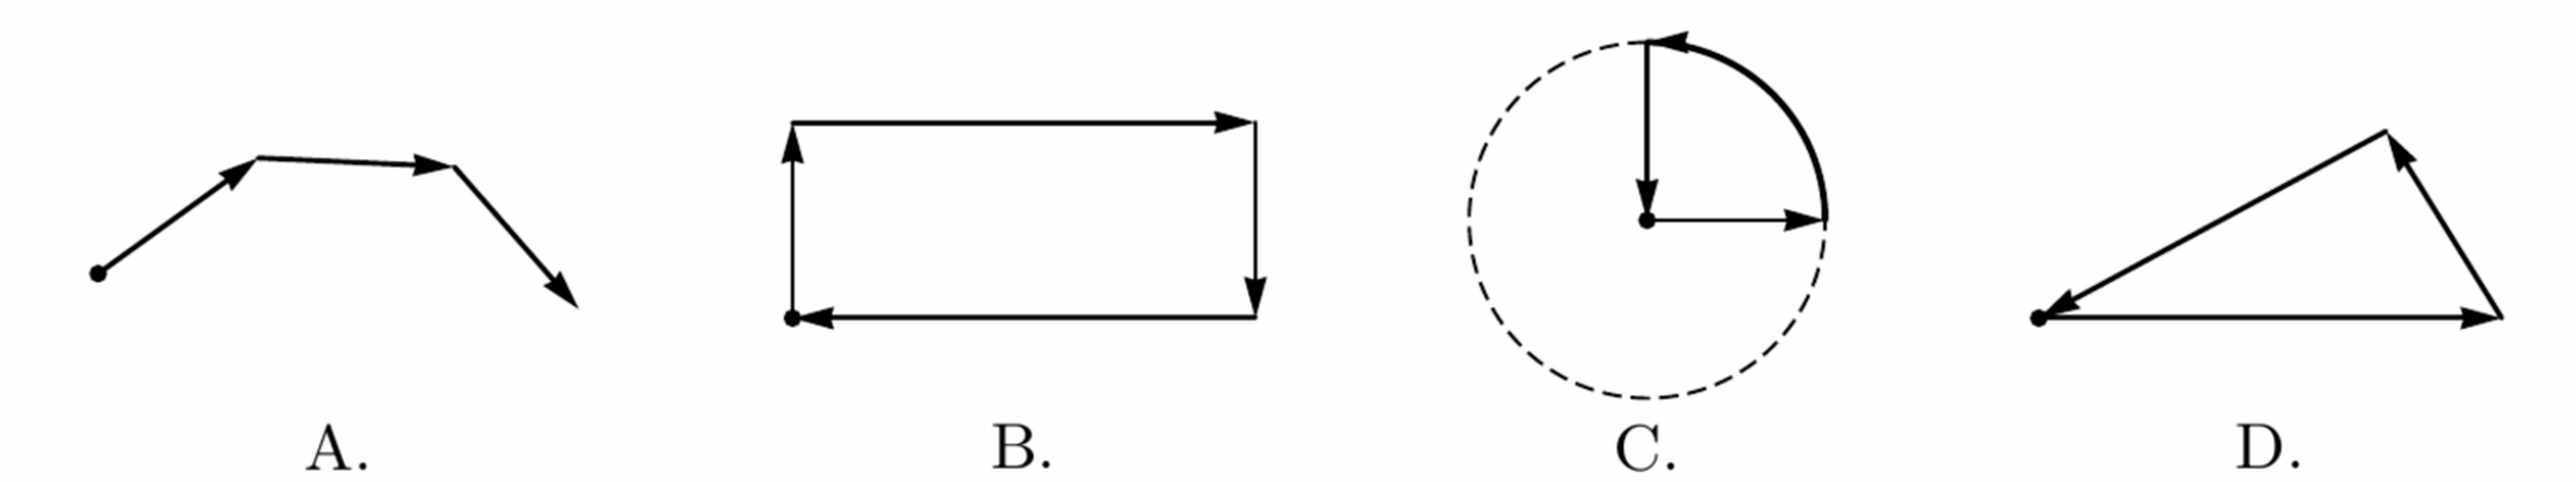
\includegraphics[width=0.86\textwidth]{figures/gao156_q14_opts.png}
\end{center}

\ifanswer
\solbegin
\step{由王老师锻炼时所走的离家距离（$S$）与行走时间（$t$）之间的函数关系图，}
\step{得在中间一段时间里，他到家的距离为定值，}
\step{故他所走的路程是一段以家为圆心的圆弧，故选 $C$.}
\solend
\fi

% === Q15 === 解析内曲线交点图（仅答案版出）；解析 4 行，故选 B
\item 已知 $a+2^a=b+\log_2 b=c+\log_3 c=k$，若 $k<1$，则\mbox{（\quad）}

\keepwithprev
A. $c<a<b$\qquad B. $a<c<b$\qquad C. $b<a<c$\qquad D. $a<b<c$

\ifanswer
\solbegin
\step{因为 $a+2^a=b+\log_2 b=c+\log_3 c=k$，}
\step{所以 $2^a=-a+k$，$\log_2 b=-b+k$，$\log_3 c=-c+k$，其中 $k<1$；}
\step{分别作出 $y=2^x$，$y=\log_2 x$，$y=\log_3 x$ 和 $y=-x+k$ 的图象，}

\begin{center}
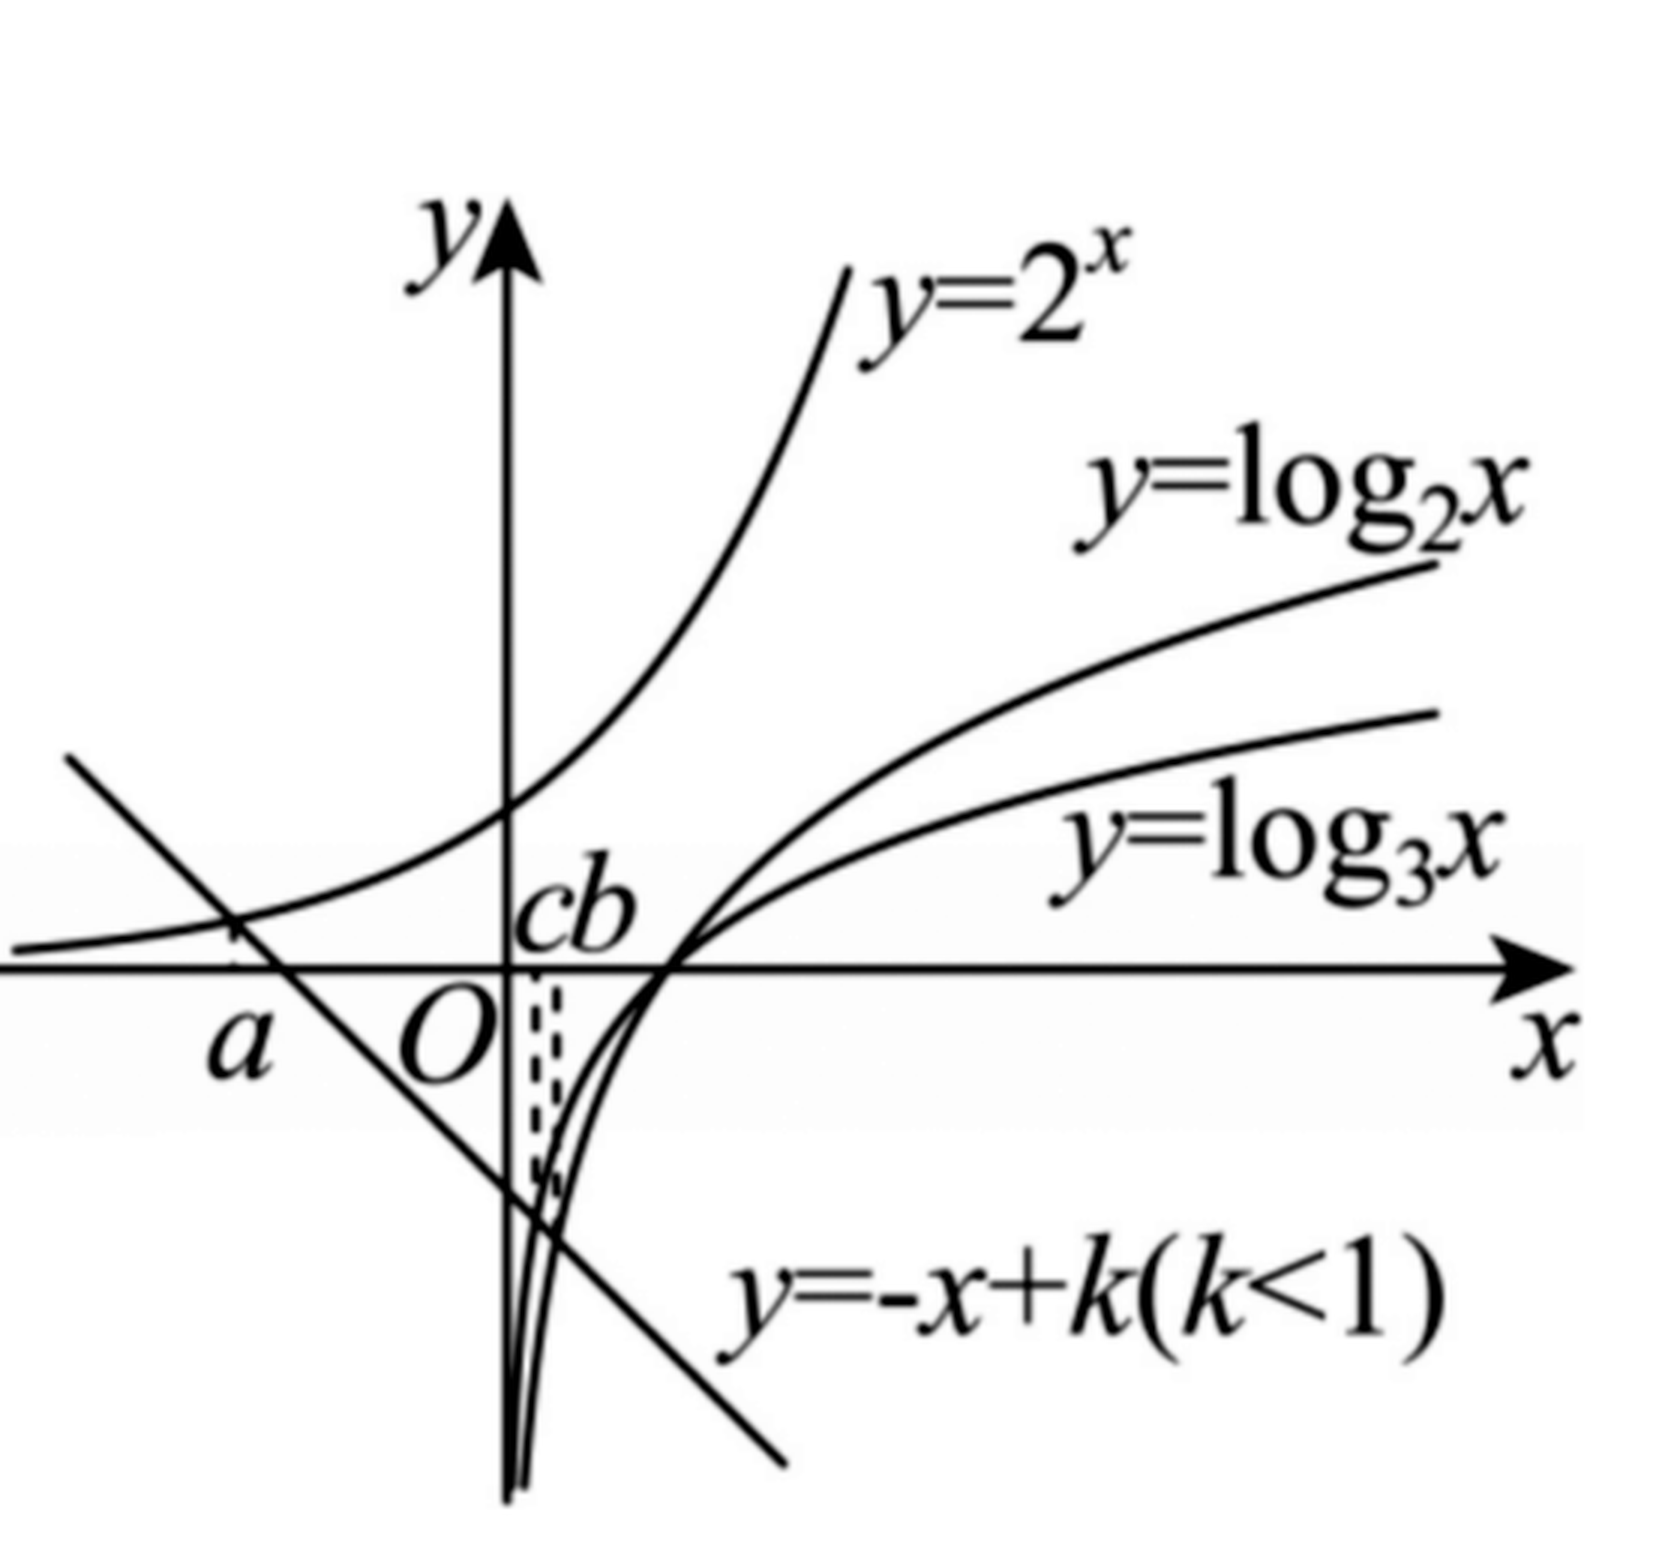
\includegraphics[width=0.52\textwidth]{figures/gao156_q15_curves.png}
\end{center}

\step{如图所示，由图象得 $a<c<b$. 故选 $B$.}
\solend
\fi

% === Q16 === ①② 文本圈数字、"一阶/二阶不动点""稳定点"自定义名词；解析 5 行，故选 A
\item 对定义域为 $I$ 的函数 $y=f(x)$，若存在 $x_0\in I$ 使得 $f(x_0)=x_0$，则称 $x_0$ 是函数 $f(x)$ 的
一阶不动点，简称不动点；若存在 $x_0\in I$ 使得 $f(f(x_0))=x_0$，则称 $x_0$ 是函数 $f(x)$ 的二阶
不动点，简称稳定点. 现有如下两个命题：①存在函数非 $y=x$ 且有无穷多个不动点；②
存在函数有无穷多个稳定点，且这些稳定点不都是不动点. 则\mbox{（\quad）}

\keepwithprev
A. ①成立，②成立\qquad\qquad B. ①成立，②不成立

C. ①不成立，②成立\qquad\qquad D. ①不成立，②不成立

\ifanswer
\solbegin
\step{①取定义在全体实数上的 $f(x)=\lvert x\rvert$，其不动点为一切非负实数，有无穷多个，}
\step{且 $f(-1)=1\ne-1$，①成立.}
\step{②取定义在全体实数上的 $g(x)=-x$，则 $g(g(x))=-(-x)=x$，}
\step{全体实数都是稳定点，而不动点只有 0，②成立.}
\step{故选 $A$.}
\solend
\fi

\end{enumerate}

\bigsec{三、解答题}

\begin{enumerate}
\setcounter{enumi}{16}

% === Q17 === $A\cap B$、$B\cap C$、\varnothing、\mid；解析 6 行
\item 设集合 $A=\{x\mid-1\leqslant x\leqslant2\}$，$B=\{x\mid2m<x<1\}$，$C=\{x\mid x<-1$ 或 $x>2\}$.

(1) 若 $A\cap B=B$，求实数 $m$ 的取值范围；

(2) 若 $B\cap C$ 中只有一个整数，求实数 $m$ 的取值范围.

\ifanswer
\solbegin
\step{(1) 当 $m\geqslant\dfrac12$ 时，$B=\varnothing$，满足 $A\cap B=B$.}
\step{当 $m<\dfrac12$ 时，$A\cap B=B$ 等价于 $2m\geqslant-1$，得 $-\dfrac12\leqslant m<\dfrac12$.}
\step{因此 $m$ 的取值范围为 $\left[-\dfrac12,+\infty\right)$.}
\step{(2) $B\cap C=\{x\mid2m<x<-1\}$，其中只有一个整数时，该整数必为 $-2$.}
\step{包含 $-2$ 且不包含 $-3$，等价于 $-3\leqslant2m<-2$，}
\step{因此 $m$ 的取值范围为 $\left[-\dfrac32,-1\right)$.}
\solend
\fi

% === Q18 === 幂函数 $x^{-\frac13}$、$m\in\R$；解析 12 行，跨 05—06 页
\item 已知幂函数 $f(x)=(3m^2-2m)x^m$（$m\in\R$）在定义域上不单调.

(1) 求函数 $f(x)$ 的解析式；

(2) 若 $f(a+1)<f(-2a+3)$，求实数 $a$ 的取值范围.

\ifanswer
\solbegin
\step{(1) 由幂函数的定义，$3m^2-2m=1$，即 $(3m+1)(m-1)=0$，得 $m=1$ 或 $m=-\dfrac13$.}
\step{当 $m=1$ 时，$f(x)=x$ 在定义域上单调递增，不合题意.}
\step{当 $m=-\dfrac13$ 时，$f(-1)=-1<f(1)=1$，而 $f(1)=1>f(8)=\dfrac12$，}
\step{故 $f(x)$ 在定义域上不单调.}
\step{因此 $f(x)=x^{-\frac13}$，定义域为 $(-\infty,0)\cup(0,+\infty)$.}
\step{(2) 有意义的条件为 $a\ne-1$ 且 $a\ne\dfrac32$.}
\step{当 $a<-1$ 时，$a+1<0<-2a+3$，有 $f(a+1)<0<f(-2a+3)$，}
\step{不等式成立.}
\step{当 $-1<a<\dfrac32$ 时，利用 $f(x)$ 在 $(0,+\infty)$ 上单调递减，}
\step{原不等式等价于 $a+1>-2a+3$，得 $\dfrac23<a<\dfrac32$.}
\step{当 $a>\dfrac32$ 时，$f(a+1)>0>f(-2a+3)$，不等式不成立.}
\step{所以 $a\in(-\infty,-1)\cup\left(\dfrac23,\dfrac32\right)$.}
\solend
\fi

% === Q19 === 两套解法（法一红字 \stepm，法二无标签）；\Delta 与 \subseteq；解析 21 行，跨 06—08 页
\item 已知 $a,c\in\R$，函数 $f(x)=\dfrac{x^2+(3a+1)x+c}{x+a}$.

(1) 若 $a=0$，求函数的定义域，并判断是否存在 $c$ 使得 $y=f(x)$ 图像关于原点对称，说明理由；

(2) 若函数过点 $(1,3)$，且函数 $y=f(x)$ 与 $x$ 轴负半轴有两个不同交点，求此时 $c$ 的值和 $a$ 的取值范围.

\ifanswer
\solbegin
\step{(1) 当 $a=0$ 时，$f(x)=\dfrac{x^2+(3a+1)x+c}{x+a}=\dfrac{x^2+x+c}{x}=x+\dfrac cx+1$，}
\step{故定义域为 $(-\infty,0)\cup(0,+\infty)$；}
\step{若存在实数 $c$，使得函数 $f(x)$ 为奇函数，则必有 $f(x)+f(-x)=0$，}
\step{而 $x+\dfrac cx+1+(-x)+\dfrac c{-x}+1=2\ne0$，}
\step{所以不存在实数 $c$，使得函数 $f(x)$ 为奇函数；}
\step{(2) 函数 $f(x)$ 的图像过点 $(1,3)$，则 $f(1)=\dfrac{1+(3a+1)+c}{1+a}=\dfrac{3a+c+2}{a+1}=3$，}
\step{解得 $c=1$，所以 $f(x)=\dfrac{x^2+(3a+1)x+1}{x+a}$，}
\stepm{法一：}{令 $f(x)=0$，则 $x^2+(3a+1)x+1=0$，此时方程有两不等负根，}
\step{则有 $\begin{cases}\Delta=(3a+1)^2-4>0\\-(3a+1)<0\end{cases}\Rightarrow\begin{cases}a>\dfrac13\text{ 或 }a<-1\\a>-\dfrac13\end{cases}\Rightarrow a>\dfrac13$，}
\step{注意到分母 $x+a\ne0$，则 $x\ne-a$，}
\step{若 $x=-a$ 也是方程 $x^2+(3a+1)x+1=0$ 的解，}
\step{代入方程 $(-a)^2+(3a+1)(-a)+1=0\Rightarrow2a^2+a-1=(a+1)(2a-1)=0$，}
\step{解得 $a=-1$ 或 $a=\dfrac12$，从而 $a\ne\dfrac12$，}
\step{综上，实数 $a$ 的取值范围为 $\left(\dfrac13,\dfrac12\right)\cup\left(\dfrac12,+\infty\right)$.}
\step{令 $g(x)=x^2+(3a+1)x+1$，与 $x$ 轴负半轴有两个交点，}
\step{则 $\begin{cases}-(3a+1)<0\\\Delta=(3a+1)^2-4>0\end{cases}\Rightarrow a>\dfrac13$.}
\step{注意到分母 $x+a\ne0$，则 $x\ne-a$，}
\step{若 $x=-a$ 也是方程 $x^2+(3a+1)x+1=0$ 的解，}
\step{代入方程 $(-a)^2+(3a+1)(-a)+1=0\Rightarrow2a^2+a-1=(a+1)(2a-1)=0$，}
\step{解得 $a=-1$ 或 $a=\dfrac12$，从而 $a\ne\dfrac12$，}
\step{综上，实数 $a$ 的取值范围为 $\left(\dfrac13,\dfrac12\right)\cup\left(\dfrac12,+\infty\right)$.}
\solend
\fi

% === Q20 === $Q$ 常数段 80000 照录；cases 与基本不等式；解析 10 行，跨 08—09 页
\item 某工厂生产某种零件的固定成本为 20000 元，每生产一个零件要增加投入 100 元，已知
总收入 $Q$（单位：元）关于产量 $x$（单位：个）满足函数：$Q=\begin{cases}400x-\dfrac12x^2,&0\leqslant x\leqslant400\\80000,&x>400\end{cases}$.

(1) 将利润 $P$（单位：元）表示为产量 $x$ 的函数；（总收入$=$总成本$+$利润）

(2) 当产量为何值时，零件的单位利润最大？最大单位利润是多少元？（单位利润$=$利润$\div$产量）

\ifanswer
\solbegin
\step{(1) 当 $0\leqslant x\leqslant400$ 时，}
\step{$P(x)=400x-\dfrac12x^2-20000-100x=-\dfrac12x^2+300x-20000$，}
\step{当 $x>400$ 时，$P(x)=80000-100x-20000=60000-100x$，}
\step{故 $P(x)=\begin{cases}-\dfrac12x^2+300x-20000,&0\leqslant x\leqslant400\\60000-100x,&x>400\end{cases}$.}
\step{(2) 设零件的单位利润为 $g(x)$，则 $g(x)=\begin{cases}-\dfrac12x-\dfrac{20000}{x}+300,&0\leqslant x\leqslant400\\\dfrac{60000}{x}-100,&x>400\end{cases}$，}
\step{当 $0\leqslant x\leqslant400$ 时，}
\step{$g(x)=300-\left(\dfrac12x+\dfrac{20000}{x}\right)\leqslant300-2\sqrt{\dfrac x2\cdot\dfrac{20000}{x}}=100$，}
\step{当且仅当 $\dfrac x2=\dfrac{20000}{x}$，即 $x=200$ 时取等号，}
\step{当 $x>400$ 时，$g(x)=\dfrac{60000}{x}-100$，此时无最值，}
\step{故当产量为 200 个，零件的单位利润最大，最大单位利润是 100 元.}
\solend
\fi

% === Q21 === 上升集定义、$D(x_0)=\{d\in\R\mid\cdots\}$、①②③ 文本圈数字、
%            \subseteq 带下划线、$-2^{-x}$；解析 19 行，跨 09—10 页
\item 已知函数 $y=f(x)$ 的定义域为 $\R$. 对任意 $x_0\in\R$，定义集合
$D(x_0)=\{d\in\R\mid f(x_0+d)>f(x_0)\}$，则称 $D(x_0)$ 为函数 $y=f(x)$ 在 $x_0$ 处的上升集.

(1) 若 $f(x)=1-x$，求 $D(-1)$；

(2) 若 $f(x)=\begin{cases}2^x,&x<0\\0,&x=0\\-2^{-x},&x>0\end{cases}$，求 $D(x)$；

(3) 设 $y=f(x)$ 满足：①当 $x<0$ 时，$f(x)=2^x$；②若 $f(x_1)\leqslant f(x_2)$，则
$D(x_2)\subseteq D(x_1)$；③当 $0<x<1$ 时，$f(x)<f(0)$. 证明：$f(0)\geqslant1$.

\ifanswer
\solbegin
\step{(1) $f(-1+d)>f(-1)\Leftrightarrow2-d>2\Leftrightarrow d<0$，所以 $D(-1)=(-\infty,0)$.}
\step{(2) 函数在 $(-\infty,0)$、$(0,+\infty)$ 上分别严格递增，}
\step{且这两个区间上的函数值分别为正、负，$f(0)=0$.}
\step{当 $x<0$ 时，$f(x+d)>f(x)\Leftrightarrow x<x+d<0\Leftrightarrow0<d<-x$，}
\step{当 $x=0$ 时，$f(d)>f(0)\Leftrightarrow d<0$，}
\step{当 $x>0$ 时，$f(x+d)>f(x)\Leftrightarrow x+d\leqslant0$ 或 $x+d>x$}
\step{$\Leftrightarrow d\leqslant-x$ 或 $d>0$，}
\step{因此 $D(x)=\begin{cases}(0,-x),&x<0\\(-\infty,0),&x=0\\(-\infty,-x]\cup(0,+\infty),&x>0\end{cases}$.}
\step{(3) 任取 $a\in(-1,0)$，}
\step{令 $d=-\dfrac a2$，则 $0<d<1$，且 $f(a+d)=2^{\frac a2}>2^a=f(a)$，}
\step{所以 $d\in D(a)$；}
\step{由③，$f(d)<f(0)$，所以 $d\notin D(0)$.}
\step{若 $f(0)\leqslant f(a)$，由②得 $D(a)\subseteq D(0)$，与上述结论矛盾.}
\step{因此，对任意 $a\in(-1,0)$，都有 $f(0)>2^a$.}
\step{特别地 $f(0)>2^{-\frac12}>0$.}
\step{若 $f(0)<1$，取 $a=\dfrac12\log_2 f(0)$，则 $-\dfrac14<a<0$，且}
\step{$2^a=\sqrt{f(0)}>f(0)$，}
\step{与 $f(0)>2^a$ 矛盾.}
\step{所以 $f(0)\geqslant1$.}
\solend
\fi

\end{enumerate}

\end{document}
"
%
% ① 原始材料：微信公众号"魔都数学加油站"文章，连载"27学年高一156"，原文标题
% "27学年高一156——2026-2027年上海市大同中学高一上期中"；
% 原文链接：https://mp.weixin.qq.com/s/xLtS5tyjCPJIWCIBohwGvw 。
% 正文为 10 张 PNG 页（01/02/03/04/05/06/07/08/09/10 各页分辨率混排
% 2560×3620 与 4762×6735，逐页按各自分辨率裁图核对）。
% 体例：讲评版——填空 3—12（10 题）、选择 13—16（4 题）、解答 17—21（5 题），
% 共 19 题，自第 3 题起编（1、2 未印在本篇）；Q3 只印【答案】、其余 18 题
% 逐题印【解析】（逐题核实，见 ②）。题目、答案、解析均据原图转录；卷面粉红色
% 水印"魔都数学加油站"及公众号页脚未录入。
%
% 卷首标题：原卷印作"2026-2027 年大同中学高一上期中"，年份区间按全稿惯例排 en dash；
% 原卷卷面未印副标题，本稿按同期中卷知识模块口径补出"集合与常用逻辑用语、不等式、函数"。
%
% ② 与原卷的排版差异：
%   ① 原文从第 3 题起，本稿保留原题号；共 19 题三节，解答题 5 题到 21；
%   ② 混合体例：第 3 题只印【答案】、无【解析】，按 高一140 第 5 题／高一145
%      第 3 题／高一151 第 7 题成例另提 \ans{}、不补造解析；其余 18 题印
%      【解析】、用 \solbegin…\solend；四道选择题答案在解析末句"故选 C／C／B／A"
%      （逐个放大复核）、括号 \mbox{（\quad）} 留空、不另提 \ans{}；答案版
%      【答案】/【解析】标记数 = 19 = 全卷题数（1 个 \ans ＋ 18 个 \solbegin）；
%   ③ 原卷卷面未印副标题，本稿按知识模块口径补出；
%   ④ 原卷填空横线按全稿惯例排 \blankline[4.4em]；选择题括号排 \mbox{（\quad）}、
%      选项段前按惯例各加 \keepwithprev；解答题不留作答区、不加 \anspace
%      （原卷为讲评版，109—113 起全稿不用 \anspace）；
%   ⑤ 数集：Q3"$x\in\R$"、Q18"$m\in\R$"、Q19"$a,c\in\R$"、Q21"定义域为 \R"
%      "任意 $x_0\in\R$""$d\in\R$"原卷印正体粗体 R，按全稿惯例归一 \R；
%      绝对值排 \lvert…\rvert（Q11 $\lvert2^x-1\rvert$、Q16 $\lvert x\rvert$），
%      集合描述竖线排 \mid（Q17 $A=\{x\mid\cdots\}$、Q21 $D(x_0)=\{d\in\R\mid\cdots\}$），
%      空集 \varnothing（Q17"$B=\varnothing$"），不等号按全稿惯例排 \leqslant／\geqslant；
%   ⑥ 子集符号逐处照录不统一：Q21 (3) 题干"$D(x_2)\subseteq D(x_1)$"与解析
%      "$D(a)\subseteq D(0)$"均印带下划线 ⊆，照录 \subseteq；本卷无单线 ⊂ 用例；
%   ⑦ 判别式：Q19 两套解法"$\Delta=(3a+1)^2-4>0$"印等腰偏高 \Delta，照录 \Delta；
%      本卷无扁三角 \triangle 用例；
%   ⑧ 红字照录为黑体：Q19 (2) 解析第一套解法行首"法一："原卷排**红色加粗**，
%      按 高一53 成例排 \stepm{法一：}{…}（加粗着色、不改黑色基调），全库无红字
%      排字先例、本稿不引入红色定义，文件头注明；第二套解法原卷直接以
%      "令 $g(x)=x^2+(3a+1)x+1$，与 $x$ 轴负半轴有两个交点，"另起，
%      **未印"法二："标签**（逐页像素级复核：07 页仅 1437—1475 一处红字，
%      08 页无红字），照录为普通 \step、不补造标签；
%   ⑨ 文本模式圈数字逐处照录：Q12 解析 ①② 两情形、Q16 两则命题与四个选项及
%      解析的 ①②、Q21 (3) 三条件 ①②③ 与解析"由③""由②"，均为印刷圈数字
%      （非 \textcircled、非数学模式），计入圈数字实测；
%   ⑩ 自定义名词照录：Q16"一阶不动点，简称不动点""二阶不动点，简称稳定点"、
%      Q21"上升集"；Q16 题干"存在函数非 $y=x$ 且有无穷多个不动点"照录；
%   ⑪ 中文弯引号照录：Q3""存在 $x\in\R$，$x^3-1\leqslant0$" 否定形式为"、
%      Q13"使"$\dfrac{x+1}{1-x}\geqslant0$"成立的必要不充分条件是"；
%      注释里一律 ASCII 引号；数学式内 CJK 用 \text{}（Q19 cases 内"或"）；
%   ⑫ 半角逗号在数学组之间是全稿惯例、非笔误，逐处照录（$a,c$、$x,y$、$a,b$
%      之类）；行末西文句点 ASCII `.`；行中全角逗号／顿号照录；
%   ⑬ 复杂式照录别简化：Q6 $\left(\dfrac{1}{\sqrt a}\right)^{\frac27}\cdot\sqrt[7]{a^3}$
%      与解析 $a^{\frac{12}{7}-\frac17+\frac37}$、Q8 $2\sqrt4+5=9$（$\sqrt4$ 未化简）、
%      Q9 $\left(\sqrt x+\dfrac{1}{\sqrt x}\right)^3$、Q12 $\dfrac{4a-(2-a)^2}{4a}$、
%      Q18 $f(8)=\dfrac12$、Q19 $2a^2+a-1=(a+1)(2a-1)=0$、Q20 $Q$ 的常数段
%      $80000$（不是 $80000-100x$）与 $2\sqrt{\dfrac x2\cdot\dfrac{20000}{x}}$、
%      Q21 $f(a+d)=2^{\frac a2}>2^a=f(a)$ 与 $2^a=\sqrt{f(0)}>f(0)$ 等；
%      \left…\right 不得拆到不同 $…$ 组（Q5 $\left(0,\dfrac12\right)$、
%      Q12 $\left[0,4+2\sqrt3\right)$、Q17 $\left[-\dfrac12,+\infty\right)$、
%      Q19 $\left(\dfrac13,\dfrac12\right)\cup\left(\dfrac12,+\infty\right)$、
%      Q20 $\left(\dfrac12x+\dfrac{20000}{x}\right)$ 等）；cases 块整体算一个印刷行；
%   ⑭ 一条 \step = 原卷解析的一个印刷行；别并折行、别拆行。跨页续印按题合并
%      （Q6 的 01 页上下题干重复印、Q8 的 01—02 页、Q12 的 02—03 页、
%      Q15 的 04 页上下、Q16 的 04—05 页、Q17 的 05 页上下、Q18 的 05—06 页、
%      Q19 的 06—08 页、Q20 的 08—09 页、Q21 的 09—10 页）；
%      跨半页重叠行（Q12 的"②若 …"、Q18 的"原不等式等价于 …"、
%      Q20 的"【解析】(1) 当 $0\leqslant x\leqslant400$ 时，"、Q21 的
%      "【解析】(1) $f(-1+d)>f(-1)\cdots$"与"与 $f(0)>2^a$ 矛盾."）
%      只算一个印刷行；
%   ⑮ 配图：全卷 3 组（逐页通读 10 页确认）——
%      · Q14 题干 S-t 梯形图（03 页右下，离家距离 S 对行走时间 t），题目配图、
%        三版都出，裁 figures/gao156_q14_st.png；
%      · Q14 四幅路线选项（04 页上部，A/B/C/D 四幅横排、C 为以家为圆心的圆弧），
%        题目配图、三版都出，合并成一张，裁 figures/gao156_q14_opts.png；
%      · Q15 解析内曲线交点图（04 页右下，$y=2^x$、$y=\log_2x$、$y=\log_3x$
%        与 $y=-x+k$），仅答案版出，裁 figures/gao156_q15_curves.png；
%      3 图均取自原卷截图，去粉色水印、去色、3×~4× LANCZOS 放大；
%      Q14 题干"题干＋两图"整块用 \needvspace 守卫推走（守卫放 \item 之前，
%      见 高一154 Q15／高一136 Q13 成例）；Q15 解析内图放 \ifanswer 内
%      \solbegin…\solend 的两 \step 之间（高一108 第 6 题／高一154 附加题 2 成例）；
%      其余各页逐页确认无其它题目配图、无解析配图、无表格；10 页下半仅水印、无正文。
%
% ③ 行数复核：一条 \step = 原卷解析的一个印刷行，cases 块作一个印刷行计。
%   逐题数（主会话逐页核对定稿）：Q3：0（只印【答案】、提 \ans{}，不计入 \step 账）；
%   Q4：1；Q5：1；Q6：1；Q7：1；Q8：3；Q9：2；Q10：2；Q11：5；Q12：12；
%   Q13：3；Q14：3；Q15：4；Q16：5；Q17：6；Q18：12；Q19：21；Q20：10；Q21：19。
%   合计 111 行（110 条 \step ＋ 1 条 \stepm），与原卷逐题印刷行相等。
%   全卷 19 题：Q3 一处 \ans{} ＋ 其余 18 题设 \solbegin…\solend，
%   答案版【答案】/【解析】标记数 = 19 = 全卷题数。
%
% ④ 页码分布（供回原图复核）：
%   卷首标题＋"一、填空题"＋Q3 题干＋【答案】、Q4 题干＋解析 1 行、
%   Q5 题干＋解析 1 行、Q6 题干首行在 01 页上半；
%   Q6 题干（重复印）＋解析 1 行、Q7 题干＋解析 1 行、Q8 题干＋解析前 2 行
%   在 01 页下半；Q8 解析末行、Q9 题干＋解析 2 行、Q10 题干＋解析 2 行、
%   Q11 题干首行在 02 页上半；Q11 题干（重复印）＋解析 5 行、
%   Q12 题干＋解析首行在 02 页下半；Q12 解析中 9 行在 03 页上半；
%   Q12 解析末 2 行＋"二、选择题"标题＋Q13 题干＋选项＋解析 3 行＋
%   Q14 题干首行在 03 页下半；Q14 题干续行＋四幅选项图＋解析 3 行＋
%   Q15 题干＋选项＋解析前 2 行＋Q16 题干在 04 页上半；
%   Q15 解析后 2 行＋曲线图＋Q16 选项＋解析前 2 行在 04 页下半；
%   Q16 解析后 3 行＋"三、解答题"标题＋Q17 题干＋两问＋解析 (1) 3 行
%   在 05 页上半；Q17 解析 (2) 3 行＋Q18 题干＋两问＋解析 (1) 首 2 行
%   在 05 页下半；Q18 解析 (1)(2) 中 8 行在 06 页上半；Q18 解析末 2 行＋
%   Q19 题干＋两问＋解析 (1) 首行在 06 页下半；Q19 解析 (1) 后 4 行＋
%   (2) 前 2 行＋法一 2 行在 07 页上半；法一后 5 行＋法二前 3 行在 07 页下半；
%   法二后 4 行＋Q20 题干＋两问＋解析 (1) 首行在 08 页上半；
%   Q20 解析 (1) 后 3 行＋(2) 前 5 行在 08 页下半；Q20 解析 (2) 末 2 行＋
%   Q21 题干＋三问＋解析 (1) 首行在 09 页上半；Q21 解析 (1)（重复印）＋
%   (2) 8 行＋(3) 首行在 09 页下半；Q21 (3) 解析中 8 行在 10 页上半；
%   Q21 (3) 末 2 行在 10 页下半。本稿按题连排，不丢行、不并折行；
%   全卷末题为第 21 题，无附加题节。
%
\documentclass[a4paper,11pt]{article}
\usepackage{common}

\begin{document}

\examtitlest[3]{2026--2027 年大同中学高一上期中}{集合与常用逻辑用语、不等式、函数}

\bigsec{一、填空题}

\begin{enumerate}
\setcounter{enumi}{2}

% === Q3 === 只印【答案】、无【解析】；R 正体粗体 \R；中文弯引号照录
\item “存在 $x\in\R$，$x^3-1\leqslant0$” 否定形式为\blankline[4.4em].

\ifanswer
\ans{对任意 $x\in\R$，$x^3-1>0$}
\fi

% === Q4 === 解析 1 行
\item 若实数 $a>0$ 且 $a\ne1$，函数 $y=a^{x-3}+1$ 的图像恒过定点 $P$，则点 $P$ 的坐标为\blankline[4.4em].

\ifanswer
\solbegin
\step{当 $x=3$ 时，$y=a^0+1=2$，与 $a$ 无关，所以定点为 $P(3,2)$.}
\solend
\fi

% === Q5 === 解析 1 行
\item 函数 $y=\dfrac{1}{3^x+2}$ 的值域是\blankline[4.4em].

\ifanswer
\solbegin
\step{$3^x\in(0,+\infty)$，因此 $3^x+2\in(2,+\infty)$，值域为 $\left(0,\dfrac12\right)$.}
\solend
\fi

% === Q6 === 根式嵌套照录；解析 1 行；题干跨 01 页上下重复印
\item 已知 $a>0$，化简 $a^{\frac{12}{7}}\cdot\left(\dfrac{1}{\sqrt a}\right)^{\frac27}\cdot\sqrt[7]{a^3}=$\blankline[4.4em].

\ifanswer
\solbegin
\step{原式 $=a^{\frac{12}{7}}\cdot a^{-\frac17}\cdot a^{\frac37}=a^{\frac{12}{7}-\frac17+\frac37}=a^2$.}
\solend
\fi

% === Q7 === 换底公式；解析 1 行
\item 已知 $\log_5 3=a$，用 $a$ 的代数式表示 $\log_{15}125=$\blankline[4.4em].

\ifanswer
\solbegin
\step{$\log_{15}125=\dfrac{\log_5 125}{\log_5 15}=\dfrac{3}{1+\log_5 3}=\dfrac{3}{1+a}$.}
\solend
\fi

% === Q8 === 基本不等式，$\sqrt4$ 照录未化简；解析 3 行，跨 01—02 页
\item 已知 $x>0$，$y>0$，且 $4x+y=xy$，则 $x+y$ 的最小值为\blankline[4.4em].

\ifanswer
\solbegin
\step{由 $4x+y=xy$，得 $\dfrac4y+\dfrac1x=1$，}
\step{则 $x+y=(x+y)\left(\dfrac4y+\dfrac1x\right)=\dfrac{4x}{y}+\dfrac yx+1+4\geqslant2\sqrt4+5=9$，}
\step{当且仅当 $\dfrac{4x}{y}=\dfrac yx$，即 $x=3$，$y=6$ 时取等号，故最小值为 9.}
\solend
\fi

% === Q9 === 解析 2 行
\item 已知 $x^{-1}+x=7$（$x>0$），则 $x^{\frac32}+x^{-\frac32}$ 的值为\blankline[4.4em].

\ifanswer
\solbegin
\step{$x>0$，有 $\sqrt x+\dfrac{1}{\sqrt x}=\sqrt{x+\dfrac1x+2}=3$，}
\step{所以 $x^{\frac32}+x^{-\frac32}=\left(\sqrt x+\dfrac{1}{\sqrt x}\right)^3-3\left(\sqrt x+\dfrac{1}{\sqrt x}\right)=27-9=18$.}
\solend
\fi

% === Q10 === $x_{\min}$；解析 2 行
\item 已知不等式 $x>\dfrac{2a+1}{a-1}$ 对任意的 $x\in[1,2]$ 恒成立，则实数 $a$ 的取值范围是\blankline[4.4em].

\ifanswer
\solbegin
\step{不等式 $x>\dfrac{2a+1}{a-1}$ 对任意的 $x\in[1,2]$ 恒成立，得 $\dfrac{2a+1}{a-1}<x_{\min}=1$，}
\step{即有 $\dfrac{a+2}{a-1}<0$，解得 $-2<a<1$，则实数 $a$ 的取值范围是 $(-2,1)$.}
\solend
\fi

% === Q11 === 分段函数 cases 与绝对值 \lvert…\rvert；解析 5 行
\item 已知函数 $f(x)=\begin{cases}\lvert2^x-1\rvert-a,&x\leqslant2\\\dfrac{3}{x-1}-a,&x>2\end{cases}$，若函数 $y=f(x)$ 图像与 $x$ 轴有三个不同交点，则实数 $a$ 的取值范围是\blankline[4.4em].

\ifanswer
\solbegin
\step{令 $g(x)=f(x)+a$.}
\step{在 $(-\infty,0)$、$[0,2]$、$(2,+\infty)$ 上，$g(x)$ 均严格单调，}
\step{值域依次为 $(0,1)$、$[0,3]$、$(0,3)$.}
\step{每段至多有一个交点，因而恰有三个不同交点，}
\step{当且仅当 $a\in(0,1)\cap[0,3]\cap(0,3)=(0,1)$.}
\solend
\fi

% === Q12 === ①② 文本圈数字、对称轴与最小值式照录；解析 12 行，跨 02—03 页
\item 已知函数 $f(x)=ax^2-(2-a)x+1$，$g(x)=x$，若对于任意实数 $x$，$f(x)$ 与 $g(x)$ 至少有一个为正数，则实数 $a$ 的取值范围是\blankline[4.4em].

\ifanswer
\solbegin
\step{当 $x>0$ 时，$g(x)>0$；当 $x<0$ 时，$g(x)<0$；}
\step{当 $x=0$ 时，$f(0)=1>0$；}
\step{因为对于任意实数 $x$，$f(x)$ 与 $g(x)$ 至少有一个为正数，}
\step{当 $x<0$ 时，因为 $g(x)<0$，所以 $f(x)=ax^2-(2-a)x+1>0$ 恒成立，}
\step{当 $a<0$ 时，显然不成立，}
\step{当 $a=0$ 时，$f(x)=-2x+1>0$，对 $x<0$ 时恒成立，满足题意，}
\step{当 $a>0$ 时，函数图象开口向上，对称轴 $x=\dfrac{2-a}{2a}$，}
\step{①若 $\dfrac{2-a}{2a}\geqslant0$，即 $0<a\leqslant2$ 时，函数 $f(x)$ 在 $(-\infty,0)$ 上严格减，$f(0)=1$，}
\step{故 $f(x)>0$ 对 $x<0$ 时恒成立，满足题意；}
\step{②若 $\dfrac{2-a}{2a}<0$，即 $a>2$ 时，$f(x)_{\min}=f\left(\dfrac{2-a}{2a}\right)=\dfrac{4a-(2-a)^2}{4a}>0$，}
\step{解得 $4-2\sqrt3<a<4+2\sqrt3$，所以 $2<a<4+2\sqrt3$.}
\step{综上，$0\leqslant a<4+2\sqrt3$，故实数 $a$ 的取值范围是 $\left[0,4+2\sqrt3\right)$.}
\solend
\fi

\end{enumerate}

\bigsec{二、选择题}

\begin{enumerate}
\setcounter{enumi}{12}

% === Q13 === 必要不充分条件；cases 块；解析 3 行，故选 C
\item 使 “$\dfrac{x+1}{1-x}\geqslant0$” 成立的必要不充分条件是\mbox{（\quad）}

\keepwithprev
A. $-1\leqslant x<1$\qquad B. $x\leqslant-1$ 或 $x>1$\qquad C. $-1\leqslant x\leqslant1$\qquad D. $x\leqslant-1$ 或 $x\geqslant0$

\ifanswer
\solbegin
\step{由不等式 $\dfrac{x+1}{1-x}\geqslant0$ 得 $\begin{cases}(x+1)(1-x)\geqslant0\\1-x\ne0\end{cases}$，解得 $-1\leqslant x<1$，}
\step{由题意结合选项，$-1\leqslant x<1\Rightarrow-1\leqslant x\leqslant1$ 成立，反之不成立，}
\step{所以 $-1\leqslant x\leqslant1$ 是 $\dfrac{x+1}{1-x}\geqslant0$ 成立的必要不充分条件. 故选 $C$.}
\solend
\fi

% === Q14 === 题干 S-t 图＋四幅路线选项（题目配图，三版都出）；守卫放 \item 之前；解析 3 行，故选 C
\needvspace{9cm}
\item 如图是王老师锻炼时所走的离家距离（$S$）与行走时间（$t$）之间的函数关系图，若
用黑点表示王老师家的位置，则王老师行走的路线可能是\mbox{（\quad）}

\begin{center}
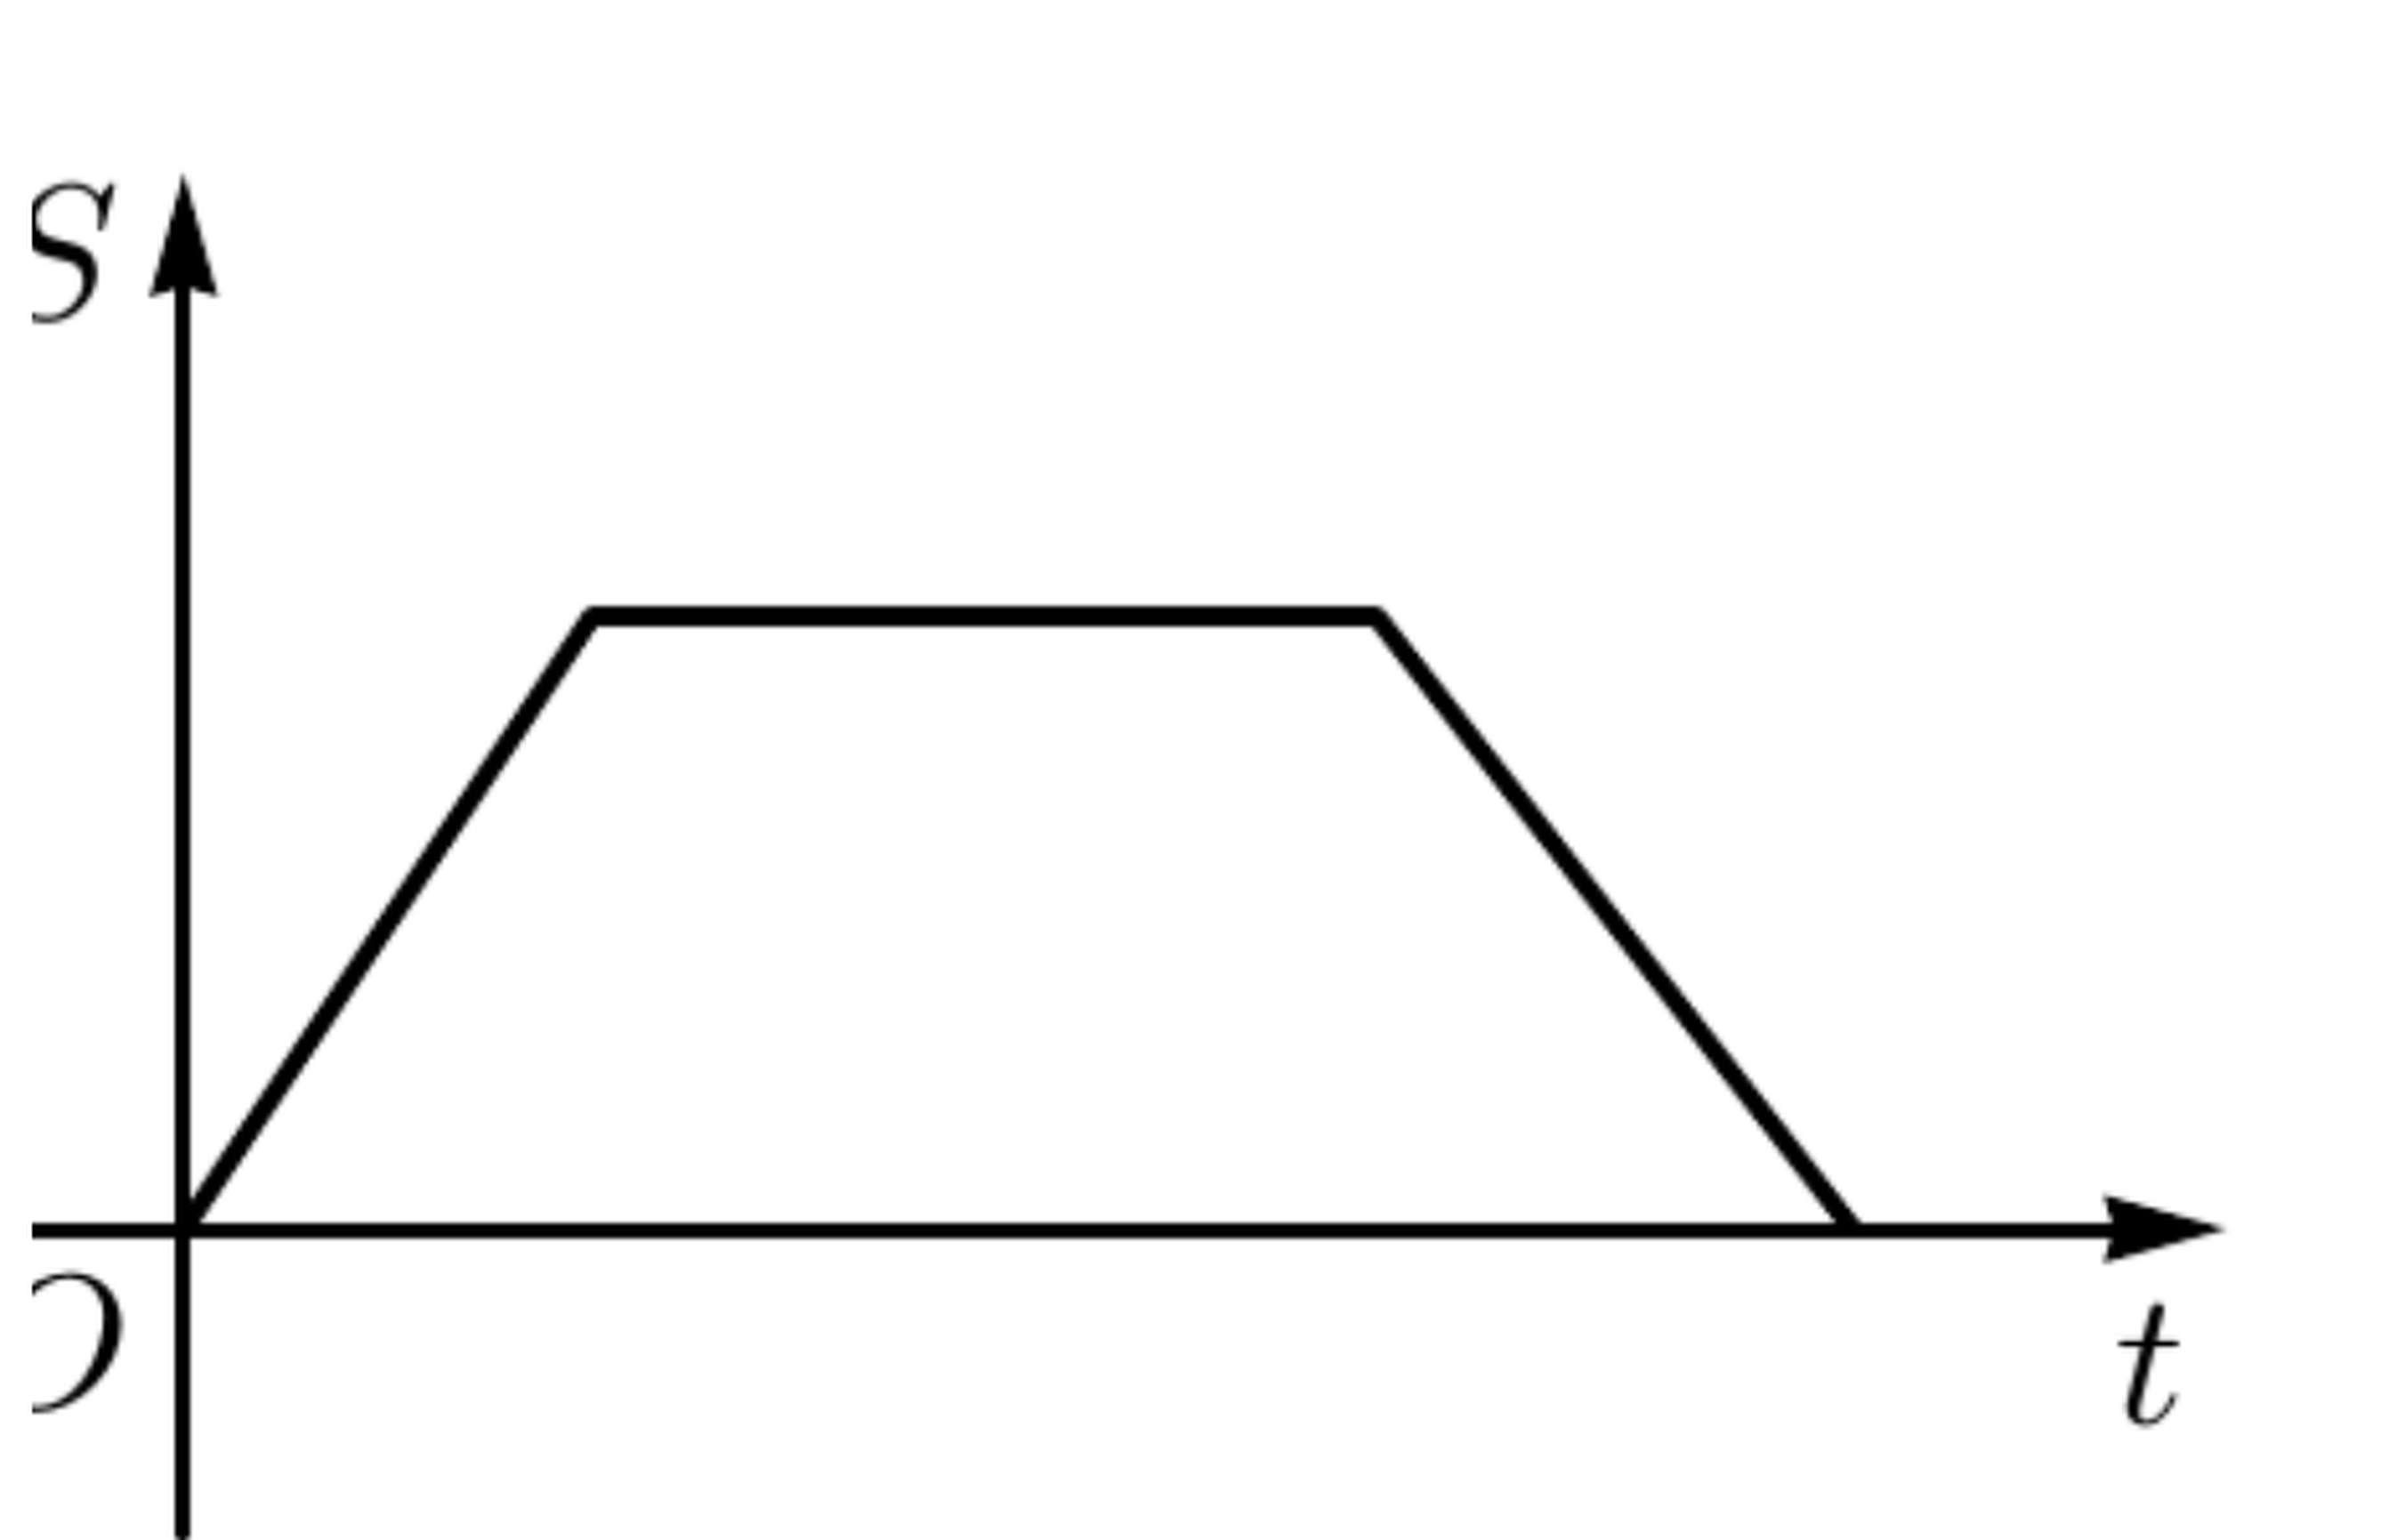
\includegraphics[width=0.34\textwidth]{figures/gao156_q14_st.png}
\end{center}

\keepwithprev
\begin{center}
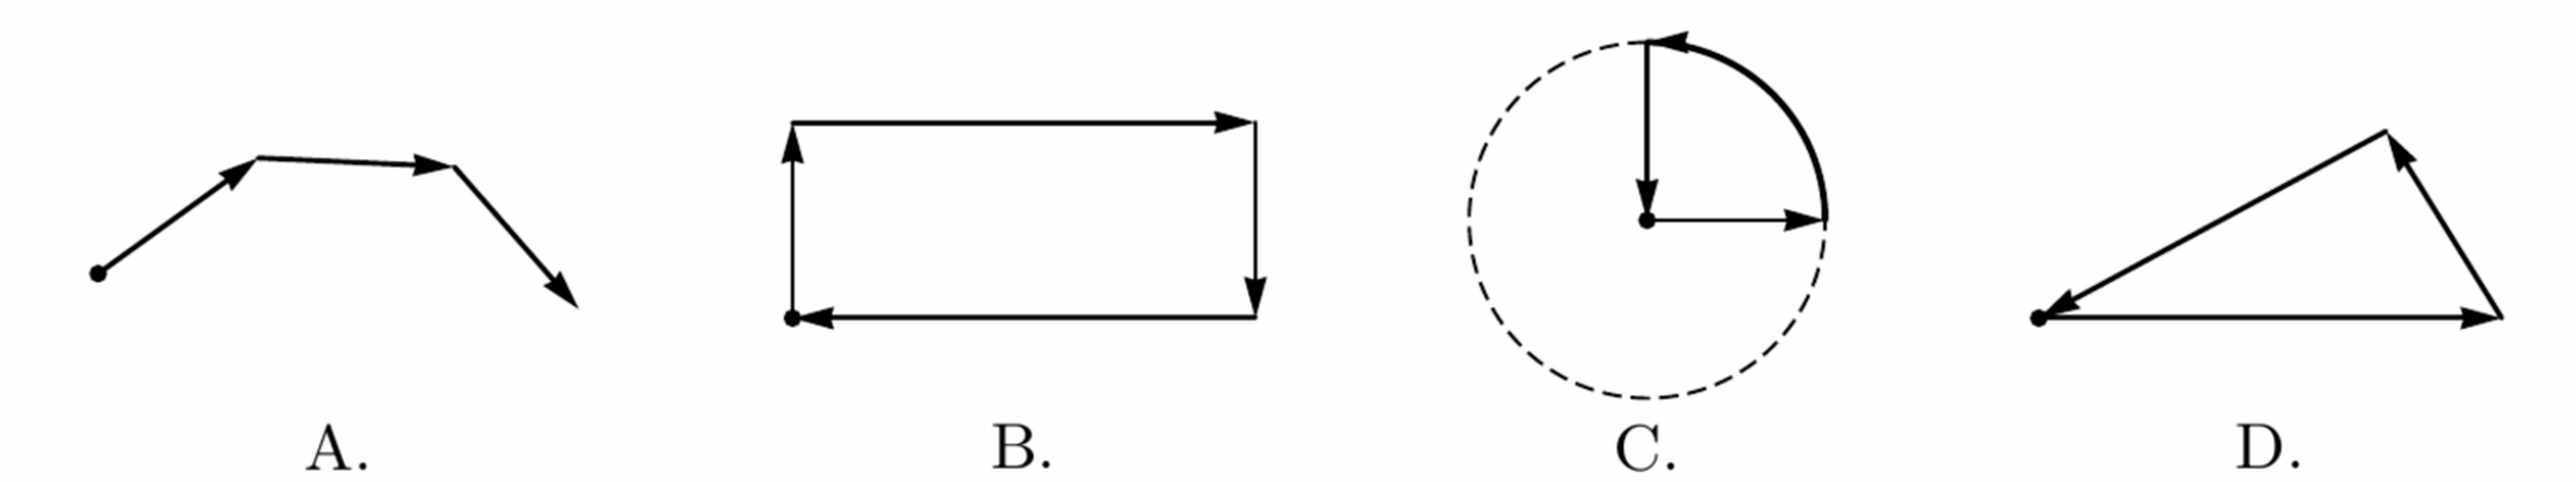
\includegraphics[width=0.86\textwidth]{figures/gao156_q14_opts.png}
\end{center}

\ifanswer
\solbegin
\step{由王老师锻炼时所走的离家距离（$S$）与行走时间（$t$）之间的函数关系图，}
\step{得在中间一段时间里，他到家的距离为定值，}
\step{故他所走的路程是一段以家为圆心的圆弧，故选 $C$.}
\solend
\fi

% === Q15 === 解析内曲线交点图（仅答案版出）；解析 4 行，故选 B
\item 已知 $a+2^a=b+\log_2 b=c+\log_3 c=k$，若 $k<1$，则\mbox{（\quad）}

\keepwithprev
A. $c<a<b$\qquad B. $a<c<b$\qquad C. $b<a<c$\qquad D. $a<b<c$

\ifanswer
\solbegin
\step{因为 $a+2^a=b+\log_2 b=c+\log_3 c=k$，}
\step{所以 $2^a=-a+k$，$\log_2 b=-b+k$，$\log_3 c=-c+k$，其中 $k<1$；}
\step{分别作出 $y=2^x$，$y=\log_2 x$，$y=\log_3 x$ 和 $y=-x+k$ 的图象，}

\begin{center}
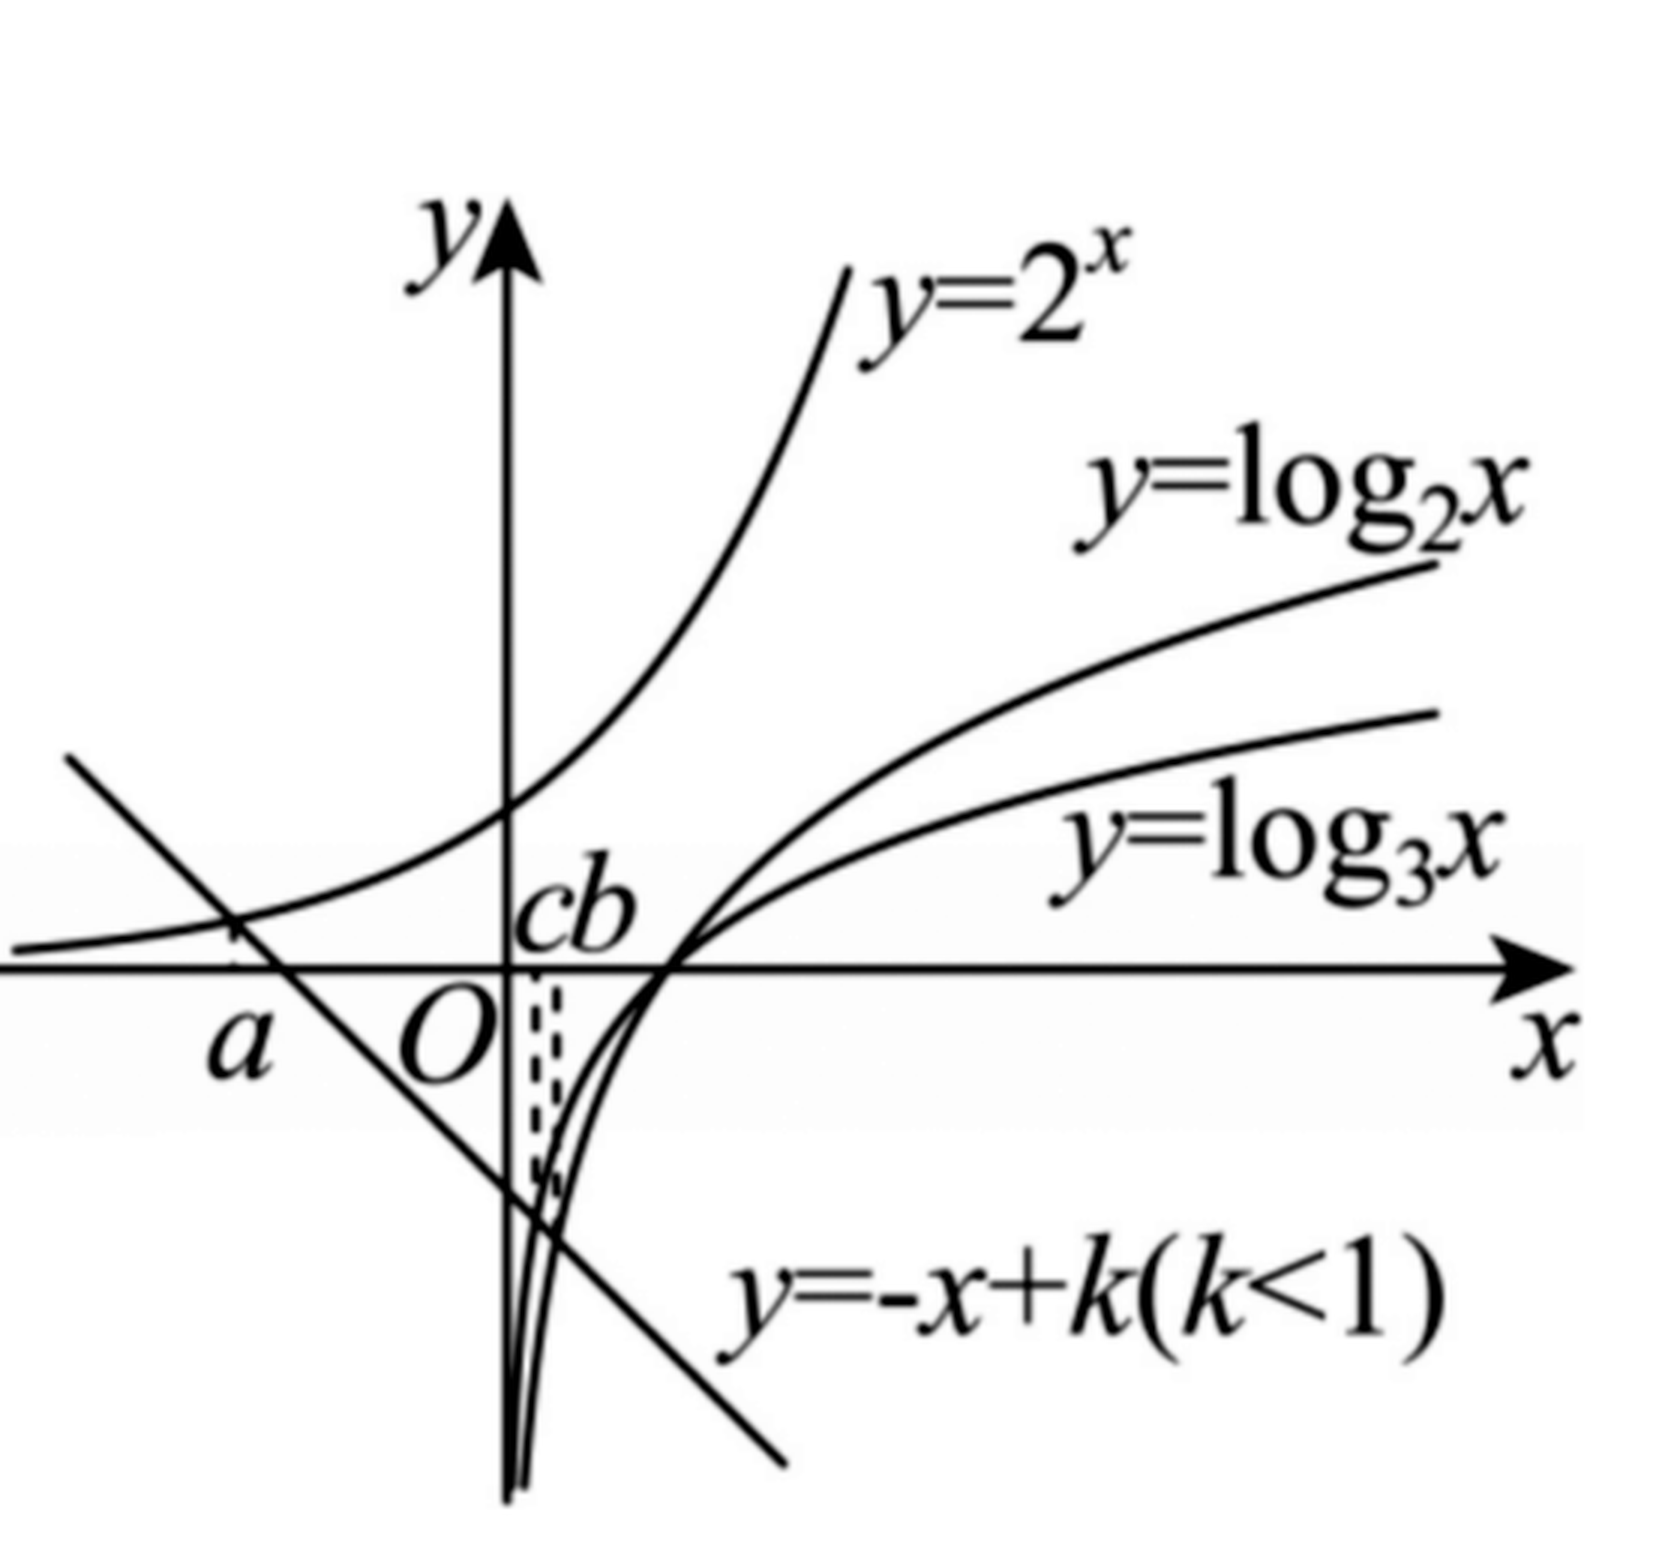
\includegraphics[width=0.52\textwidth]{figures/gao156_q15_curves.png}
\end{center}

\step{如图所示，由图象得 $a<c<b$. 故选 $B$.}
\solend
\fi

% === Q16 === ①② 文本圈数字、"一阶/二阶不动点""稳定点"自定义名词；解析 5 行，故选 A
\item 对定义域为 $I$ 的函数 $y=f(x)$，若存在 $x_0\in I$ 使得 $f(x_0)=x_0$，则称 $x_0$ 是函数 $f(x)$ 的
一阶不动点，简称不动点；若存在 $x_0\in I$ 使得 $f(f(x_0))=x_0$，则称 $x_0$ 是函数 $f(x)$ 的二阶
不动点，简称稳定点. 现有如下两个命题：①存在函数非 $y=x$ 且有无穷多个不动点；②
存在函数有无穷多个稳定点，且这些稳定点不都是不动点. 则\mbox{（\quad）}

\keepwithprev
A. ①成立，②成立\qquad\qquad B. ①成立，②不成立

C. ①不成立，②成立\qquad\qquad D. ①不成立，②不成立

\ifanswer
\solbegin
\step{①取定义在全体实数上的 $f(x)=\lvert x\rvert$，其不动点为一切非负实数，有无穷多个，}
\step{且 $f(-1)=1\ne-1$，①成立.}
\step{②取定义在全体实数上的 $g(x)=-x$，则 $g(g(x))=-(-x)=x$，}
\step{全体实数都是稳定点，而不动点只有 0，②成立.}
\step{故选 $A$.}
\solend
\fi

\end{enumerate}

\bigsec{三、解答题}

\begin{enumerate}
\setcounter{enumi}{16}

% === Q17 === $A\cap B$、$B\cap C$、\varnothing、\mid；解析 6 行
\item 设集合 $A=\{x\mid-1\leqslant x\leqslant2\}$，$B=\{x\mid2m<x<1\}$，$C=\{x\mid x<-1$ 或 $x>2\}$.

(1) 若 $A\cap B=B$，求实数 $m$ 的取值范围；

(2) 若 $B\cap C$ 中只有一个整数，求实数 $m$ 的取值范围.

\ifanswer
\solbegin
\step{(1) 当 $m\geqslant\dfrac12$ 时，$B=\varnothing$，满足 $A\cap B=B$.}
\step{当 $m<\dfrac12$ 时，$A\cap B=B$ 等价于 $2m\geqslant-1$，得 $-\dfrac12\leqslant m<\dfrac12$.}
\step{因此 $m$ 的取值范围为 $\left[-\dfrac12,+\infty\right)$.}
\step{(2) $B\cap C=\{x\mid2m<x<-1\}$，其中只有一个整数时，该整数必为 $-2$.}
\step{包含 $-2$ 且不包含 $-3$，等价于 $-3\leqslant2m<-2$，}
\step{因此 $m$ 的取值范围为 $\left[-\dfrac32,-1\right)$.}
\solend
\fi

% === Q18 === 幂函数 $x^{-\frac13}$、$m\in\R$；解析 12 行，跨 05—06 页
\item 已知幂函数 $f(x)=(3m^2-2m)x^m$（$m\in\R$）在定义域上不单调.

(1) 求函数 $f(x)$ 的解析式；

(2) 若 $f(a+1)<f(-2a+3)$，求实数 $a$ 的取值范围.

\ifanswer
\solbegin
\step{(1) 由幂函数的定义，$3m^2-2m=1$，即 $(3m+1)(m-1)=0$，得 $m=1$ 或 $m=-\dfrac13$.}
\step{当 $m=1$ 时，$f(x)=x$ 在定义域上单调递增，不合题意.}
\step{当 $m=-\dfrac13$ 时，$f(-1)=-1<f(1)=1$，而 $f(1)=1>f(8)=\dfrac12$，}
\step{故 $f(x)$ 在定义域上不单调.}
\step{因此 $f(x)=x^{-\frac13}$，定义域为 $(-\infty,0)\cup(0,+\infty)$.}
\step{(2) 有意义的条件为 $a\ne-1$ 且 $a\ne\dfrac32$.}
\step{当 $a<-1$ 时，$a+1<0<-2a+3$，有 $f(a+1)<0<f(-2a+3)$，}
\step{不等式成立.}
\step{当 $-1<a<\dfrac32$ 时，利用 $f(x)$ 在 $(0,+\infty)$ 上单调递减，}
\step{原不等式等价于 $a+1>-2a+3$，得 $\dfrac23<a<\dfrac32$.}
\step{当 $a>\dfrac32$ 时，$f(a+1)>0>f(-2a+3)$，不等式不成立.}
\step{所以 $a\in(-\infty,-1)\cup\left(\dfrac23,\dfrac32\right)$.}
\solend
\fi

% === Q19 === 两套解法（法一红字 \stepm，法二无标签）；\Delta 与 \subseteq；解析 21 行，跨 06—08 页
\item 已知 $a,c\in\R$，函数 $f(x)=\dfrac{x^2+(3a+1)x+c}{x+a}$.

(1) 若 $a=0$，求函数的定义域，并判断是否存在 $c$ 使得 $y=f(x)$ 图像关于原点对称，说明理由；

(2) 若函数过点 $(1,3)$，且函数 $y=f(x)$ 与 $x$ 轴负半轴有两个不同交点，求此时 $c$ 的值和 $a$ 的取值范围.

\ifanswer
\solbegin
\step{(1) 当 $a=0$ 时，$f(x)=\dfrac{x^2+(3a+1)x+c}{x+a}=\dfrac{x^2+x+c}{x}=x+\dfrac cx+1$，}
\step{故定义域为 $(-\infty,0)\cup(0,+\infty)$；}
\step{若存在实数 $c$，使得函数 $f(x)$ 为奇函数，则必有 $f(x)+f(-x)=0$，}
\step{而 $x+\dfrac cx+1+(-x)+\dfrac c{-x}+1=2\ne0$，}
\step{所以不存在实数 $c$，使得函数 $f(x)$ 为奇函数；}
\step{(2) 函数 $f(x)$ 的图像过点 $(1,3)$，则 $f(1)=\dfrac{1+(3a+1)+c}{1+a}=\dfrac{3a+c+2}{a+1}=3$，}
\step{解得 $c=1$，所以 $f(x)=\dfrac{x^2+(3a+1)x+1}{x+a}$，}
\stepm{法一：}{令 $f(x)=0$，则 $x^2+(3a+1)x+1=0$，此时方程有两不等负根，}
\step{则有 $\begin{cases}\Delta=(3a+1)^2-4>0\\-(3a+1)<0\end{cases}\Rightarrow\begin{cases}a>\dfrac13\text{ 或 }a<-1\\a>-\dfrac13\end{cases}\Rightarrow a>\dfrac13$，}
\step{注意到分母 $x+a\ne0$，则 $x\ne-a$，}
\step{若 $x=-a$ 也是方程 $x^2+(3a+1)x+1=0$ 的解，}
\step{代入方程 $(-a)^2+(3a+1)(-a)+1=0\Rightarrow2a^2+a-1=(a+1)(2a-1)=0$，}
\step{解得 $a=-1$ 或 $a=\dfrac12$，从而 $a\ne\dfrac12$，}
\step{综上，实数 $a$ 的取值范围为 $\left(\dfrac13,\dfrac12\right)\cup\left(\dfrac12,+\infty\right)$.}
\step{令 $g(x)=x^2+(3a+1)x+1$，与 $x$ 轴负半轴有两个交点，}
\step{则 $\begin{cases}-(3a+1)<0\\\Delta=(3a+1)^2-4>0\end{cases}\Rightarrow a>\dfrac13$.}
\step{注意到分母 $x+a\ne0$，则 $x\ne-a$，}
\step{若 $x=-a$ 也是方程 $x^2+(3a+1)x+1=0$ 的解，}
\step{代入方程 $(-a)^2+(3a+1)(-a)+1=0\Rightarrow2a^2+a-1=(a+1)(2a-1)=0$，}
\step{解得 $a=-1$ 或 $a=\dfrac12$，从而 $a\ne\dfrac12$，}
\step{综上，实数 $a$ 的取值范围为 $\left(\dfrac13,\dfrac12\right)\cup\left(\dfrac12,+\infty\right)$.}
\solend
\fi

% === Q20 === $Q$ 常数段 80000 照录；cases 与基本不等式；解析 10 行，跨 08—09 页
\item 某工厂生产某种零件的固定成本为 20000 元，每生产一个零件要增加投入 100 元，已知
总收入 $Q$（单位：元）关于产量 $x$（单位：个）满足函数：$Q=\begin{cases}400x-\dfrac12x^2,&0\leqslant x\leqslant400\\80000,&x>400\end{cases}$.

(1) 将利润 $P$（单位：元）表示为产量 $x$ 的函数；（总收入$=$总成本$+$利润）

(2) 当产量为何值时，零件的单位利润最大？最大单位利润是多少元？（单位利润$=$利润$\div$产量）

\ifanswer
\solbegin
\step{(1) 当 $0\leqslant x\leqslant400$ 时，}
\step{$P(x)=400x-\dfrac12x^2-20000-100x=-\dfrac12x^2+300x-20000$，}
\step{当 $x>400$ 时，$P(x)=80000-100x-20000=60000-100x$，}
\step{故 $P(x)=\begin{cases}-\dfrac12x^2+300x-20000,&0\leqslant x\leqslant400\\60000-100x,&x>400\end{cases}$.}
\step{(2) 设零件的单位利润为 $g(x)$，则 $g(x)=\begin{cases}-\dfrac12x-\dfrac{20000}{x}+300,&0\leqslant x\leqslant400\\\dfrac{60000}{x}-100,&x>400\end{cases}$，}
\step{当 $0\leqslant x\leqslant400$ 时，}
\step{$g(x)=300-\left(\dfrac12x+\dfrac{20000}{x}\right)\leqslant300-2\sqrt{\dfrac x2\cdot\dfrac{20000}{x}}=100$，}
\step{当且仅当 $\dfrac x2=\dfrac{20000}{x}$，即 $x=200$ 时取等号，}
\step{当 $x>400$ 时，$g(x)=\dfrac{60000}{x}-100$，此时无最值，}
\step{故当产量为 200 个，零件的单位利润最大，最大单位利润是 100 元.}
\solend
\fi

% === Q21 === 上升集定义、$D(x_0)=\{d\in\R\mid\cdots\}$、①②③ 文本圈数字、
%            \subseteq 带下划线、$-2^{-x}$；解析 19 行，跨 09—10 页
\item 已知函数 $y=f(x)$ 的定义域为 $\R$. 对任意 $x_0\in\R$，定义集合
$D(x_0)=\{d\in\R\mid f(x_0+d)>f(x_0)\}$，则称 $D(x_0)$ 为函数 $y=f(x)$ 在 $x_0$ 处的上升集.

(1) 若 $f(x)=1-x$，求 $D(-1)$；

(2) 若 $f(x)=\begin{cases}2^x,&x<0\\0,&x=0\\-2^{-x},&x>0\end{cases}$，求 $D(x)$；

(3) 设 $y=f(x)$ 满足：①当 $x<0$ 时，$f(x)=2^x$；②若 $f(x_1)\leqslant f(x_2)$，则
$D(x_2)\subseteq D(x_1)$；③当 $0<x<1$ 时，$f(x)<f(0)$. 证明：$f(0)\geqslant1$.

\ifanswer
\solbegin
\step{(1) $f(-1+d)>f(-1)\Leftrightarrow2-d>2\Leftrightarrow d<0$，所以 $D(-1)=(-\infty,0)$.}
\step{(2) 函数在 $(-\infty,0)$、$(0,+\infty)$ 上分别严格递增，}
\step{且这两个区间上的函数值分别为正、负，$f(0)=0$.}
\step{当 $x<0$ 时，$f(x+d)>f(x)\Leftrightarrow x<x+d<0\Leftrightarrow0<d<-x$，}
\step{当 $x=0$ 时，$f(d)>f(0)\Leftrightarrow d<0$，}
\step{当 $x>0$ 时，$f(x+d)>f(x)\Leftrightarrow x+d\leqslant0$ 或 $x+d>x$}
\step{$\Leftrightarrow d\leqslant-x$ 或 $d>0$，}
\step{因此 $D(x)=\begin{cases}(0,-x),&x<0\\(-\infty,0),&x=0\\(-\infty,-x]\cup(0,+\infty),&x>0\end{cases}$.}
\step{(3) 任取 $a\in(-1,0)$，}
\step{令 $d=-\dfrac a2$，则 $0<d<1$，且 $f(a+d)=2^{\frac a2}>2^a=f(a)$，}
\step{所以 $d\in D(a)$；}
\step{由③，$f(d)<f(0)$，所以 $d\notin D(0)$.}
\step{若 $f(0)\leqslant f(a)$，由②得 $D(a)\subseteq D(0)$，与上述结论矛盾.}
\step{因此，对任意 $a\in(-1,0)$，都有 $f(0)>2^a$.}
\step{特别地 $f(0)>2^{-\frac12}>0$.}
\step{若 $f(0)<1$，取 $a=\dfrac12\log_2 f(0)$，则 $-\dfrac14<a<0$，且}
\step{$2^a=\sqrt{f(0)}>f(0)$，}
\step{与 $f(0)>2^a$ 矛盾.}
\step{所以 $f(0)\geqslant1$.}
\solend
\fi

\end{enumerate}

\end{document}
"
%
% ① 原始材料：微信公众号"魔都数学加油站"文章，连载"27学年高一156"，原文标题
% "27学年高一156——2026-2027年上海市大同中学高一上期中"；
% 原文链接：https://mp.weixin.qq.com/s/xLtS5tyjCPJIWCIBohwGvw 。
% 正文为 10 张 PNG 页（01/02/03/04/05/06/07/08/09/10 各页分辨率混排
% 2560×3620 与 4762×6735，逐页按各自分辨率裁图核对）。
% 体例：讲评版——填空 3—12（10 题）、选择 13—16（4 题）、解答 17—21（5 题），
% 共 19 题，自第 3 题起编（1、2 未印在本篇）；Q3 只印【答案】、其余 18 题
% 逐题印【解析】（逐题核实，见 ②）。题目、答案、解析均据原图转录；卷面粉红色
% 水印"魔都数学加油站"及公众号页脚未录入。
%
% 卷首标题：原卷印作"2026-2027 年大同中学高一上期中"，年份区间按全稿惯例排 en dash；
% 原卷卷面未印副标题，本稿按同期中卷知识模块口径补出"集合与常用逻辑用语、不等式、函数"。
%
% ② 与原卷的排版差异：
%   ① 原文从第 3 题起，本稿保留原题号；共 19 题三节，解答题 5 题到 21；
%   ② 混合体例：第 3 题只印【答案】、无【解析】，按 高一140 第 5 题／高一145
%      第 3 题／高一151 第 7 题成例另提 \ans{}、不补造解析；其余 18 题印
%      【解析】、用 \solbegin…\solend；四道选择题答案在解析末句"故选 C／C／B／A"
%      （逐个放大复核）、括号 \mbox{（\quad）} 留空、不另提 \ans{}；答案版
%      【答案】/【解析】标记数 = 19 = 全卷题数（1 个 \ans ＋ 18 个 \solbegin）；
%   ③ 原卷卷面未印副标题，本稿按知识模块口径补出；
%   ④ 原卷填空横线按全稿惯例排 \blankline[4.4em]；选择题括号排 \mbox{（\quad）}、
%      选项段前按惯例各加 \keepwithprev；解答题不留作答区、不加 \anspace
%      （原卷为讲评版，109—113 起全稿不用 \anspace）；
%   ⑤ 数集：Q3"$x\in\R$"、Q18"$m\in\R$"、Q19"$a,c\in\R$"、Q21"定义域为 \R"
%      "任意 $x_0\in\R$""$d\in\R$"原卷印正体粗体 R，按全稿惯例归一 \R；
%      绝对值排 \lvert…\rvert（Q11 $\lvert2^x-1\rvert$、Q16 $\lvert x\rvert$），
%      集合描述竖线排 \mid（Q17 $A=\{x\mid\cdots\}$、Q21 $D(x_0)=\{d\in\R\mid\cdots\}$），
%      空集 \varnothing（Q17"$B=\varnothing$"），不等号按全稿惯例排 \leqslant／\geqslant；
%   ⑥ 子集符号逐处照录不统一：Q21 (3) 题干"$D(x_2)\subseteq D(x_1)$"与解析
%      "$D(a)\subseteq D(0)$"均印带下划线 ⊆，照录 \subseteq；本卷无单线 ⊂ 用例；
%   ⑦ 判别式：Q19 两套解法"$\Delta=(3a+1)^2-4>0$"印等腰偏高 \Delta，照录 \Delta；
%      本卷无扁三角 \triangle 用例；
%   ⑧ 红字照录为黑体：Q19 (2) 解析第一套解法行首"法一："原卷排**红色加粗**，
%      按 高一53 成例排 \stepm{法一：}{…}（加粗着色、不改黑色基调），全库无红字
%      排字先例、本稿不引入红色定义，文件头注明；第二套解法原卷直接以
%      "令 $g(x)=x^2+(3a+1)x+1$，与 $x$ 轴负半轴有两个交点，"另起，
%      **未印"法二："标签**（逐页像素级复核：07 页仅 1437—1475 一处红字，
%      08 页无红字），照录为普通 \step、不补造标签；
%   ⑨ 文本模式圈数字逐处照录：Q12 解析 ①② 两情形、Q16 两则命题与四个选项及
%      解析的 ①②、Q21 (3) 三条件 ①②③ 与解析"由③""由②"，均为印刷圈数字
%      （非 \textcircled、非数学模式），计入圈数字实测；
%   ⑩ 自定义名词照录：Q16"一阶不动点，简称不动点""二阶不动点，简称稳定点"、
%      Q21"上升集"；Q16 题干"存在函数非 $y=x$ 且有无穷多个不动点"照录；
%   ⑪ 中文弯引号照录：Q3""存在 $x\in\R$，$x^3-1\leqslant0$" 否定形式为"、
%      Q13"使"$\dfrac{x+1}{1-x}\geqslant0$"成立的必要不充分条件是"；
%      注释里一律 ASCII 引号；数学式内 CJK 用 \text{}（Q19 cases 内"或"）；
%   ⑫ 半角逗号在数学组之间是全稿惯例、非笔误，逐处照录（$a,c$、$x,y$、$a,b$
%      之类）；行末西文句点 ASCII `.`；行中全角逗号／顿号照录；
%   ⑬ 复杂式照录别简化：Q6 $\left(\dfrac{1}{\sqrt a}\right)^{\frac27}\cdot\sqrt[7]{a^3}$
%      与解析 $a^{\frac{12}{7}-\frac17+\frac37}$、Q8 $2\sqrt4+5=9$（$\sqrt4$ 未化简）、
%      Q9 $\left(\sqrt x+\dfrac{1}{\sqrt x}\right)^3$、Q12 $\dfrac{4a-(2-a)^2}{4a}$、
%      Q18 $f(8)=\dfrac12$、Q19 $2a^2+a-1=(a+1)(2a-1)=0$、Q20 $Q$ 的常数段
%      $80000$（不是 $80000-100x$）与 $2\sqrt{\dfrac x2\cdot\dfrac{20000}{x}}$、
%      Q21 $f(a+d)=2^{\frac a2}>2^a=f(a)$ 与 $2^a=\sqrt{f(0)}>f(0)$ 等；
%      \left…\right 不得拆到不同 $…$ 组（Q5 $\left(0,\dfrac12\right)$、
%      Q12 $\left[0,4+2\sqrt3\right)$、Q17 $\left[-\dfrac12,+\infty\right)$、
%      Q19 $\left(\dfrac13,\dfrac12\right)\cup\left(\dfrac12,+\infty\right)$、
%      Q20 $\left(\dfrac12x+\dfrac{20000}{x}\right)$ 等）；cases 块整体算一个印刷行；
%   ⑭ 一条 \step = 原卷解析的一个印刷行；别并折行、别拆行。跨页续印按题合并
%      （Q6 的 01 页上下题干重复印、Q8 的 01—02 页、Q12 的 02—03 页、
%      Q15 的 04 页上下、Q16 的 04—05 页、Q17 的 05 页上下、Q18 的 05—06 页、
%      Q19 的 06—08 页、Q20 的 08—09 页、Q21 的 09—10 页）；
%      跨半页重叠行（Q12 的"②若 …"、Q18 的"原不等式等价于 …"、
%      Q20 的"【解析】(1) 当 $0\leqslant x\leqslant400$ 时，"、Q21 的
%      "【解析】(1) $f(-1+d)>f(-1)\cdots$"与"与 $f(0)>2^a$ 矛盾."）
%      只算一个印刷行；
%   ⑮ 配图：全卷 3 组（逐页通读 10 页确认）——
%      · Q14 题干 S-t 梯形图（03 页右下，离家距离 S 对行走时间 t），题目配图、
%        三版都出，裁 figures/gao156_q14_st.png；
%      · Q14 四幅路线选项（04 页上部，A/B/C/D 四幅横排、C 为以家为圆心的圆弧），
%        题目配图、三版都出，合并成一张，裁 figures/gao156_q14_opts.png；
%      · Q15 解析内曲线交点图（04 页右下，$y=2^x$、$y=\log_2x$、$y=\log_3x$
%        与 $y=-x+k$），仅答案版出，裁 figures/gao156_q15_curves.png；
%      3 图均取自原卷截图，去粉色水印、去色、3×~4× LANCZOS 放大；
%      Q14 题干"题干＋两图"整块用 \needvspace 守卫推走（守卫放 \item 之前，
%      见 高一154 Q15／高一136 Q13 成例）；Q15 解析内图放 \ifanswer 内
%      \solbegin…\solend 的两 \step 之间（高一108 第 6 题／高一154 附加题 2 成例）；
%      其余各页逐页确认无其它题目配图、无解析配图、无表格；10 页下半仅水印、无正文。
%
% ③ 行数复核：一条 \step = 原卷解析的一个印刷行，cases 块作一个印刷行计。
%   逐题数（主会话逐页核对定稿）：Q3：0（只印【答案】、提 \ans{}，不计入 \step 账）；
%   Q4：1；Q5：1；Q6：1；Q7：1；Q8：3；Q9：2；Q10：2；Q11：5；Q12：12；
%   Q13：3；Q14：3；Q15：4；Q16：5；Q17：6；Q18：12；Q19：21；Q20：10；Q21：19。
%   合计 111 行（110 条 \step ＋ 1 条 \stepm），与原卷逐题印刷行相等。
%   全卷 19 题：Q3 一处 \ans{} ＋ 其余 18 题设 \solbegin…\solend，
%   答案版【答案】/【解析】标记数 = 19 = 全卷题数。
%
% ④ 页码分布（供回原图复核）：
%   卷首标题＋"一、填空题"＋Q3 题干＋【答案】、Q4 题干＋解析 1 行、
%   Q5 题干＋解析 1 行、Q6 题干首行在 01 页上半；
%   Q6 题干（重复印）＋解析 1 行、Q7 题干＋解析 1 行、Q8 题干＋解析前 2 行
%   在 01 页下半；Q8 解析末行、Q9 题干＋解析 2 行、Q10 题干＋解析 2 行、
%   Q11 题干首行在 02 页上半；Q11 题干（重复印）＋解析 5 行、
%   Q12 题干＋解析首行在 02 页下半；Q12 解析中 9 行在 03 页上半；
%   Q12 解析末 2 行＋"二、选择题"标题＋Q13 题干＋选项＋解析 3 行＋
%   Q14 题干首行在 03 页下半；Q14 题干续行＋四幅选项图＋解析 3 行＋
%   Q15 题干＋选项＋解析前 2 行＋Q16 题干在 04 页上半；
%   Q15 解析后 2 行＋曲线图＋Q16 选项＋解析前 2 行在 04 页下半；
%   Q16 解析后 3 行＋"三、解答题"标题＋Q17 题干＋两问＋解析 (1) 3 行
%   在 05 页上半；Q17 解析 (2) 3 行＋Q18 题干＋两问＋解析 (1) 首 2 行
%   在 05 页下半；Q18 解析 (1)(2) 中 8 行在 06 页上半；Q18 解析末 2 行＋
%   Q19 题干＋两问＋解析 (1) 首行在 06 页下半；Q19 解析 (1) 后 4 行＋
%   (2) 前 2 行＋法一 2 行在 07 页上半；法一后 5 行＋法二前 3 行在 07 页下半；
%   法二后 4 行＋Q20 题干＋两问＋解析 (1) 首行在 08 页上半；
%   Q20 解析 (1) 后 3 行＋(2) 前 5 行在 08 页下半；Q20 解析 (2) 末 2 行＋
%   Q21 题干＋三问＋解析 (1) 首行在 09 页上半；Q21 解析 (1)（重复印）＋
%   (2) 8 行＋(3) 首行在 09 页下半；Q21 (3) 解析中 8 行在 10 页上半；
%   Q21 (3) 末 2 行在 10 页下半。本稿按题连排，不丢行、不并折行；
%   全卷末题为第 21 题，无附加题节。
%
\documentclass[a4paper,11pt]{article}
\usepackage{common}

\begin{document}

\examtitlest[3]{2026--2027 年大同中学高一上期中}{集合与常用逻辑用语、不等式、函数}

\bigsec{一、填空题}

\begin{enumerate}
\setcounter{enumi}{2}

% === Q3 === 只印【答案】、无【解析】；R 正体粗体 \R；中文弯引号照录
\item “存在 $x\in\R$，$x^3-1\leqslant0$” 否定形式为\blankline[4.4em].

\ifanswer
\ans{对任意 $x\in\R$，$x^3-1>0$}
\fi

% === Q4 === 解析 1 行
\item 若实数 $a>0$ 且 $a\ne1$，函数 $y=a^{x-3}+1$ 的图像恒过定点 $P$，则点 $P$ 的坐标为\blankline[4.4em].

\ifanswer
\solbegin
\step{当 $x=3$ 时，$y=a^0+1=2$，与 $a$ 无关，所以定点为 $P(3,2)$.}
\solend
\fi

% === Q5 === 解析 1 行
\item 函数 $y=\dfrac{1}{3^x+2}$ 的值域是\blankline[4.4em].

\ifanswer
\solbegin
\step{$3^x\in(0,+\infty)$，因此 $3^x+2\in(2,+\infty)$，值域为 $\left(0,\dfrac12\right)$.}
\solend
\fi

% === Q6 === 根式嵌套照录；解析 1 行；题干跨 01 页上下重复印
\item 已知 $a>0$，化简 $a^{\frac{12}{7}}\cdot\left(\dfrac{1}{\sqrt a}\right)^{\frac27}\cdot\sqrt[7]{a^3}=$\blankline[4.4em].

\ifanswer
\solbegin
\step{原式 $=a^{\frac{12}{7}}\cdot a^{-\frac17}\cdot a^{\frac37}=a^{\frac{12}{7}-\frac17+\frac37}=a^2$.}
\solend
\fi

% === Q7 === 换底公式；解析 1 行
\item 已知 $\log_5 3=a$，用 $a$ 的代数式表示 $\log_{15}125=$\blankline[4.4em].

\ifanswer
\solbegin
\step{$\log_{15}125=\dfrac{\log_5 125}{\log_5 15}=\dfrac{3}{1+\log_5 3}=\dfrac{3}{1+a}$.}
\solend
\fi

% === Q8 === 基本不等式，$\sqrt4$ 照录未化简；解析 3 行，跨 01—02 页
\item 已知 $x>0$，$y>0$，且 $4x+y=xy$，则 $x+y$ 的最小值为\blankline[4.4em].

\ifanswer
\solbegin
\step{由 $4x+y=xy$，得 $\dfrac4y+\dfrac1x=1$，}
\step{则 $x+y=(x+y)\left(\dfrac4y+\dfrac1x\right)=\dfrac{4x}{y}+\dfrac yx+1+4\geqslant2\sqrt4+5=9$，}
\step{当且仅当 $\dfrac{4x}{y}=\dfrac yx$，即 $x=3$，$y=6$ 时取等号，故最小值为 9.}
\solend
\fi

% === Q9 === 解析 2 行
\item 已知 $x^{-1}+x=7$（$x>0$），则 $x^{\frac32}+x^{-\frac32}$ 的值为\blankline[4.4em].

\ifanswer
\solbegin
\step{$x>0$，有 $\sqrt x+\dfrac{1}{\sqrt x}=\sqrt{x+\dfrac1x+2}=3$，}
\step{所以 $x^{\frac32}+x^{-\frac32}=\left(\sqrt x+\dfrac{1}{\sqrt x}\right)^3-3\left(\sqrt x+\dfrac{1}{\sqrt x}\right)=27-9=18$.}
\solend
\fi

% === Q10 === $x_{\min}$；解析 2 行
\item 已知不等式 $x>\dfrac{2a+1}{a-1}$ 对任意的 $x\in[1,2]$ 恒成立，则实数 $a$ 的取值范围是\blankline[4.4em].

\ifanswer
\solbegin
\step{不等式 $x>\dfrac{2a+1}{a-1}$ 对任意的 $x\in[1,2]$ 恒成立，得 $\dfrac{2a+1}{a-1}<x_{\min}=1$，}
\step{即有 $\dfrac{a+2}{a-1}<0$，解得 $-2<a<1$，则实数 $a$ 的取值范围是 $(-2,1)$.}
\solend
\fi

% === Q11 === 分段函数 cases 与绝对值 \lvert…\rvert；解析 5 行
\item 已知函数 $f(x)=\begin{cases}\lvert2^x-1\rvert-a,&x\leqslant2\\\dfrac{3}{x-1}-a,&x>2\end{cases}$，若函数 $y=f(x)$ 图像与 $x$ 轴有三个不同交点，则实数 $a$ 的取值范围是\blankline[4.4em].

\ifanswer
\solbegin
\step{令 $g(x)=f(x)+a$.}
\step{在 $(-\infty,0)$、$[0,2]$、$(2,+\infty)$ 上，$g(x)$ 均严格单调，}
\step{值域依次为 $(0,1)$、$[0,3]$、$(0,3)$.}
\step{每段至多有一个交点，因而恰有三个不同交点，}
\step{当且仅当 $a\in(0,1)\cap[0,3]\cap(0,3)=(0,1)$.}
\solend
\fi

% === Q12 === ①② 文本圈数字、对称轴与最小值式照录；解析 12 行，跨 02—03 页
\item 已知函数 $f(x)=ax^2-(2-a)x+1$，$g(x)=x$，若对于任意实数 $x$，$f(x)$ 与 $g(x)$ 至少有一个为正数，则实数 $a$ 的取值范围是\blankline[4.4em].

\ifanswer
\solbegin
\step{当 $x>0$ 时，$g(x)>0$；当 $x<0$ 时，$g(x)<0$；}
\step{当 $x=0$ 时，$f(0)=1>0$；}
\step{因为对于任意实数 $x$，$f(x)$ 与 $g(x)$ 至少有一个为正数，}
\step{当 $x<0$ 时，因为 $g(x)<0$，所以 $f(x)=ax^2-(2-a)x+1>0$ 恒成立，}
\step{当 $a<0$ 时，显然不成立，}
\step{当 $a=0$ 时，$f(x)=-2x+1>0$，对 $x<0$ 时恒成立，满足题意，}
\step{当 $a>0$ 时，函数图象开口向上，对称轴 $x=\dfrac{2-a}{2a}$，}
\step{①若 $\dfrac{2-a}{2a}\geqslant0$，即 $0<a\leqslant2$ 时，函数 $f(x)$ 在 $(-\infty,0)$ 上严格减，$f(0)=1$，}
\step{故 $f(x)>0$ 对 $x<0$ 时恒成立，满足题意；}
\step{②若 $\dfrac{2-a}{2a}<0$，即 $a>2$ 时，$f(x)_{\min}=f\left(\dfrac{2-a}{2a}\right)=\dfrac{4a-(2-a)^2}{4a}>0$，}
\step{解得 $4-2\sqrt3<a<4+2\sqrt3$，所以 $2<a<4+2\sqrt3$.}
\step{综上，$0\leqslant a<4+2\sqrt3$，故实数 $a$ 的取值范围是 $\left[0,4+2\sqrt3\right)$.}
\solend
\fi

\end{enumerate}

\bigsec{二、选择题}

\begin{enumerate}
\setcounter{enumi}{12}

% === Q13 === 必要不充分条件；cases 块；解析 3 行，故选 C
\item 使 “$\dfrac{x+1}{1-x}\geqslant0$” 成立的必要不充分条件是\mbox{（\quad）}

\keepwithprev
A. $-1\leqslant x<1$\qquad B. $x\leqslant-1$ 或 $x>1$\qquad C. $-1\leqslant x\leqslant1$\qquad D. $x\leqslant-1$ 或 $x\geqslant0$

\ifanswer
\solbegin
\step{由不等式 $\dfrac{x+1}{1-x}\geqslant0$ 得 $\begin{cases}(x+1)(1-x)\geqslant0\\1-x\ne0\end{cases}$，解得 $-1\leqslant x<1$，}
\step{由题意结合选项，$-1\leqslant x<1\Rightarrow-1\leqslant x\leqslant1$ 成立，反之不成立，}
\step{所以 $-1\leqslant x\leqslant1$ 是 $\dfrac{x+1}{1-x}\geqslant0$ 成立的必要不充分条件. 故选 $C$.}
\solend
\fi

% === Q14 === 题干 S-t 图＋四幅路线选项（题目配图，三版都出）；守卫放 \item 之前；解析 3 行，故选 C
\needvspace{9cm}
\item 如图是王老师锻炼时所走的离家距离（$S$）与行走时间（$t$）之间的函数关系图，若
用黑点表示王老师家的位置，则王老师行走的路线可能是\mbox{（\quad）}

\begin{center}
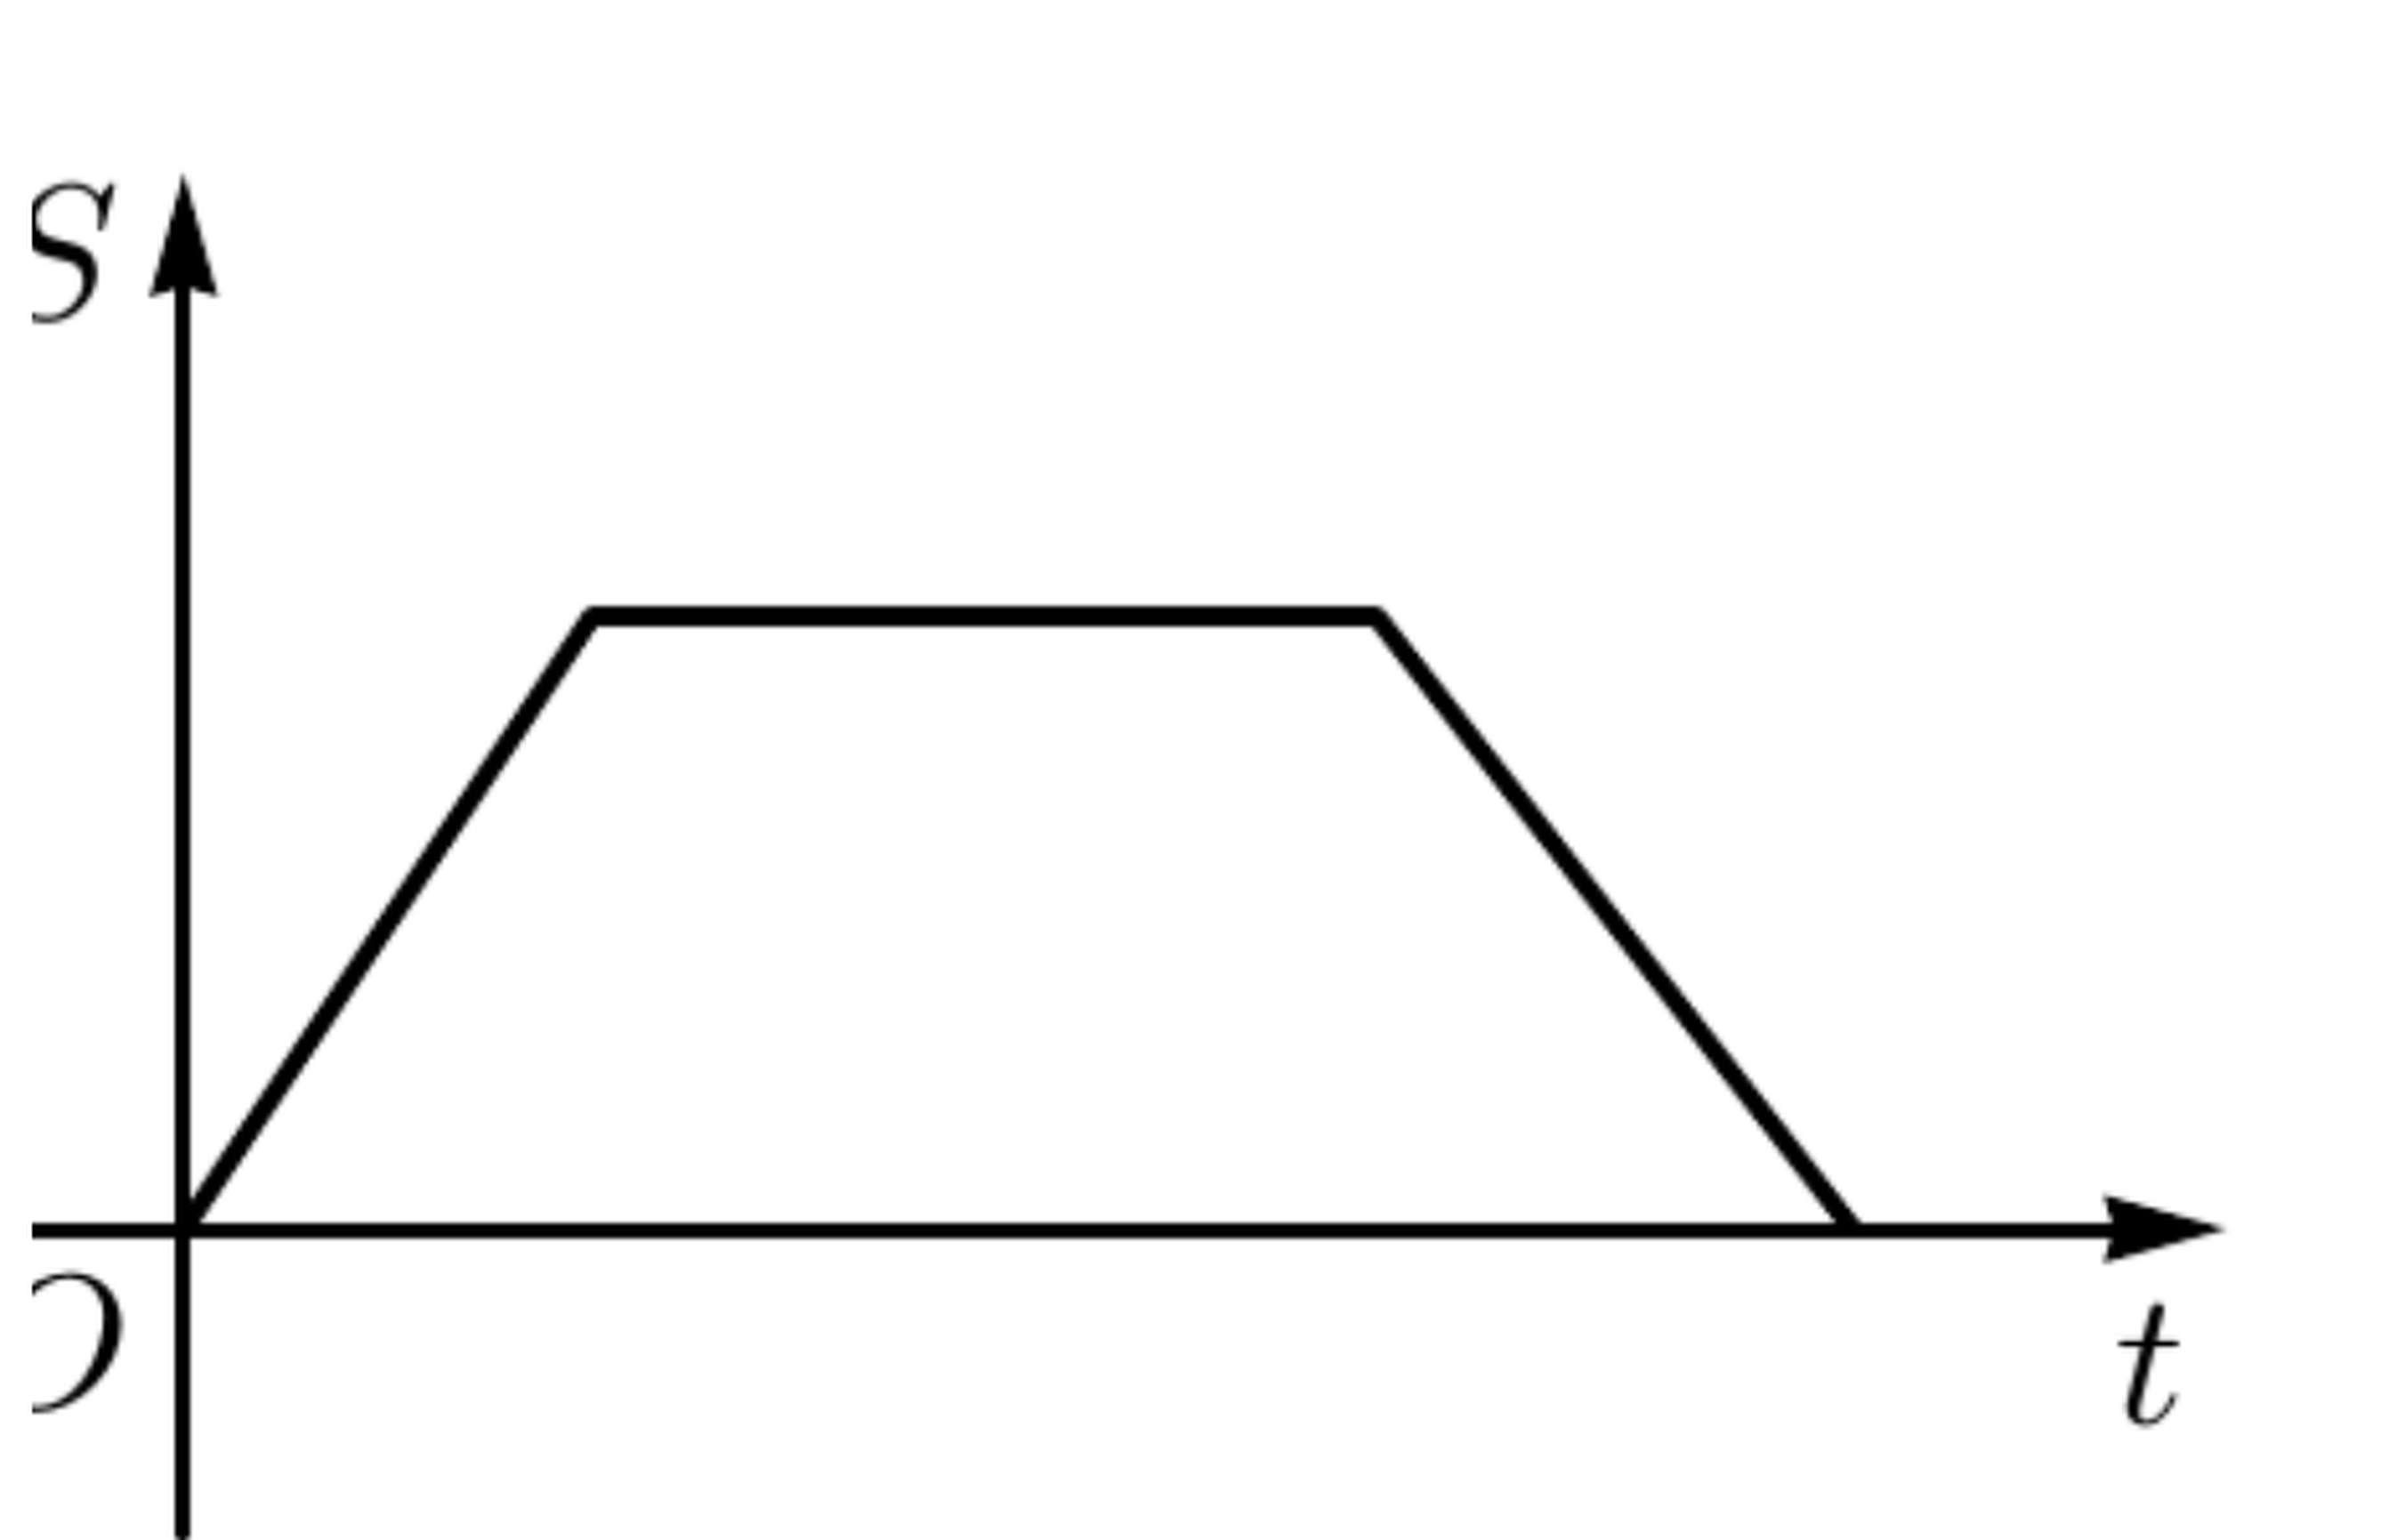
\includegraphics[width=0.34\textwidth]{figures/gao156_q14_st.png}
\end{center}

\keepwithprev
\begin{center}
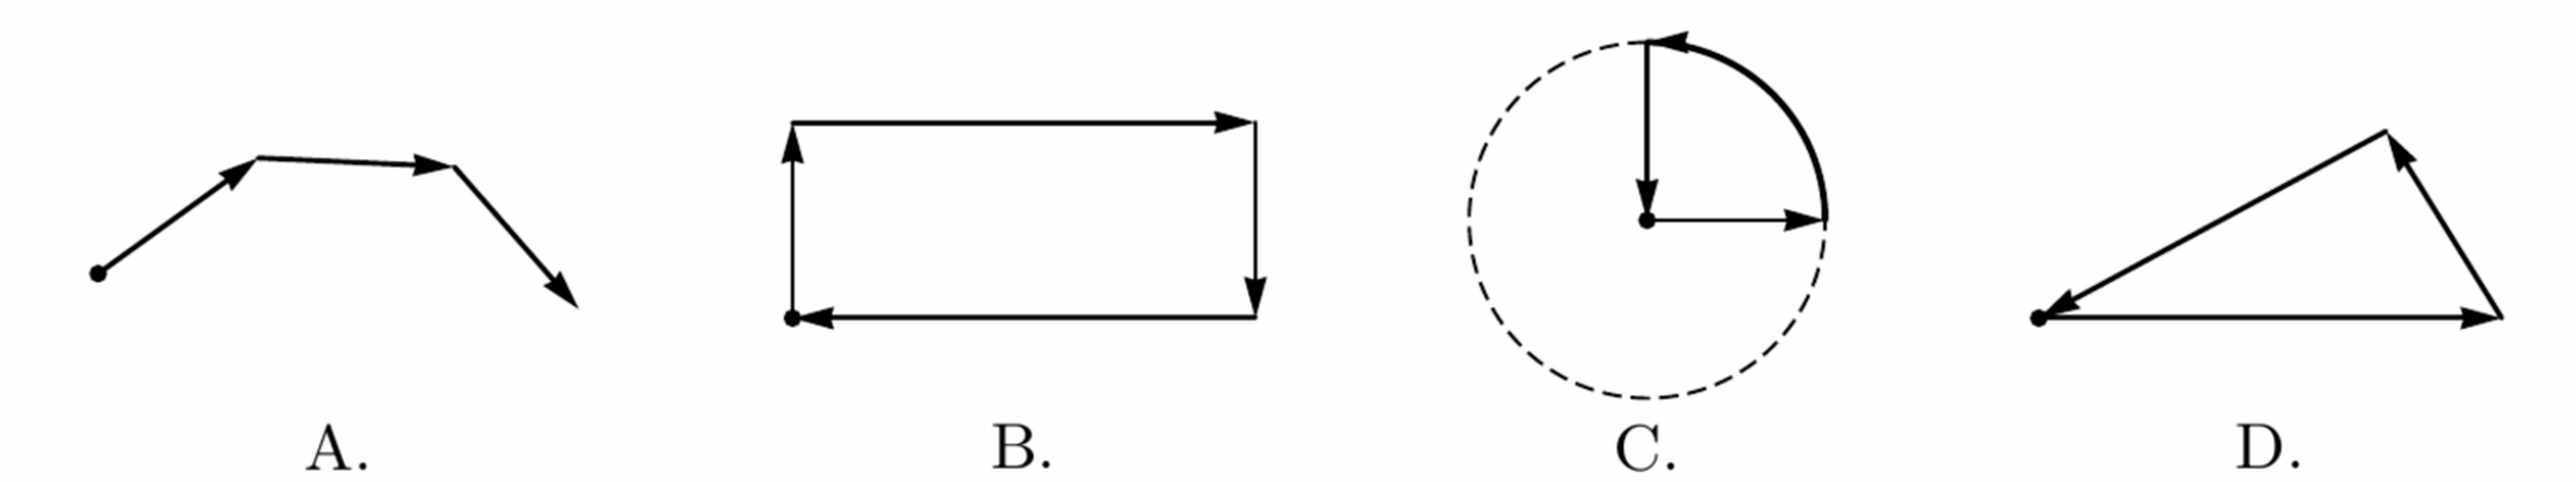
\includegraphics[width=0.86\textwidth]{figures/gao156_q14_opts.png}
\end{center}

\ifanswer
\solbegin
\step{由王老师锻炼时所走的离家距离（$S$）与行走时间（$t$）之间的函数关系图，}
\step{得在中间一段时间里，他到家的距离为定值，}
\step{故他所走的路程是一段以家为圆心的圆弧，故选 $C$.}
\solend
\fi

% === Q15 === 解析内曲线交点图（仅答案版出）；解析 4 行，故选 B
\item 已知 $a+2^a=b+\log_2 b=c+\log_3 c=k$，若 $k<1$，则\mbox{（\quad）}

\keepwithprev
A. $c<a<b$\qquad B. $a<c<b$\qquad C. $b<a<c$\qquad D. $a<b<c$

\ifanswer
\solbegin
\step{因为 $a+2^a=b+\log_2 b=c+\log_3 c=k$，}
\step{所以 $2^a=-a+k$，$\log_2 b=-b+k$，$\log_3 c=-c+k$，其中 $k<1$；}
\step{分别作出 $y=2^x$，$y=\log_2 x$，$y=\log_3 x$ 和 $y=-x+k$ 的图象，}

\begin{center}
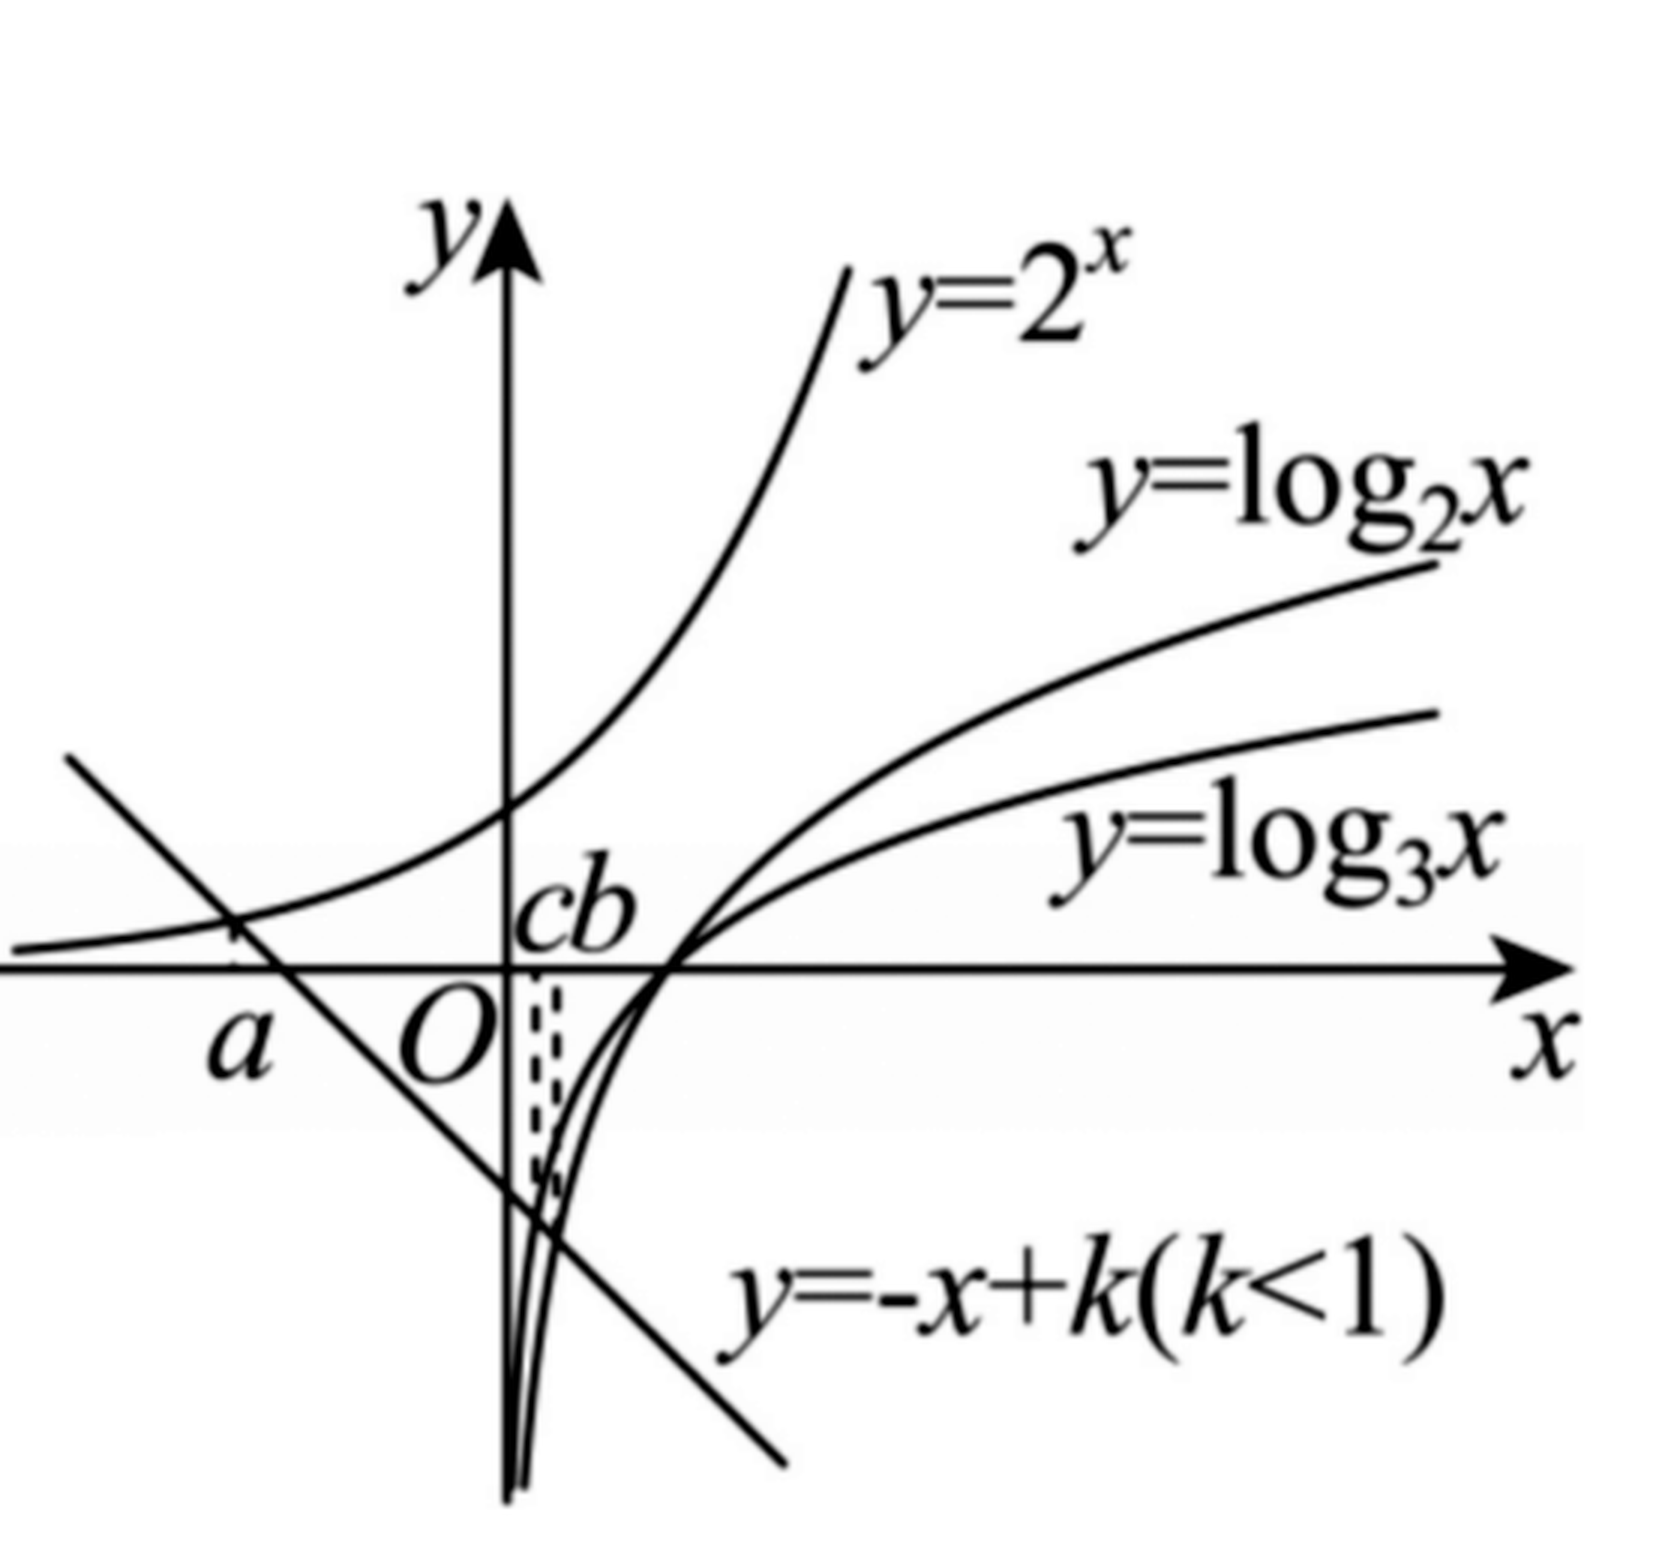
\includegraphics[width=0.52\textwidth]{figures/gao156_q15_curves.png}
\end{center}

\step{如图所示，由图象得 $a<c<b$. 故选 $B$.}
\solend
\fi

% === Q16 === ①② 文本圈数字、"一阶/二阶不动点""稳定点"自定义名词；解析 5 行，故选 A
\item 对定义域为 $I$ 的函数 $y=f(x)$，若存在 $x_0\in I$ 使得 $f(x_0)=x_0$，则称 $x_0$ 是函数 $f(x)$ 的
一阶不动点，简称不动点；若存在 $x_0\in I$ 使得 $f(f(x_0))=x_0$，则称 $x_0$ 是函数 $f(x)$ 的二阶
不动点，简称稳定点. 现有如下两个命题：①存在函数非 $y=x$ 且有无穷多个不动点；②
存在函数有无穷多个稳定点，且这些稳定点不都是不动点. 则\mbox{（\quad）}

\keepwithprev
A. ①成立，②成立\qquad\qquad B. ①成立，②不成立

C. ①不成立，②成立\qquad\qquad D. ①不成立，②不成立

\ifanswer
\solbegin
\step{①取定义在全体实数上的 $f(x)=\lvert x\rvert$，其不动点为一切非负实数，有无穷多个，}
\step{且 $f(-1)=1\ne-1$，①成立.}
\step{②取定义在全体实数上的 $g(x)=-x$，则 $g(g(x))=-(-x)=x$，}
\step{全体实数都是稳定点，而不动点只有 0，②成立.}
\step{故选 $A$.}
\solend
\fi

\end{enumerate}

\bigsec{三、解答题}

\begin{enumerate}
\setcounter{enumi}{16}

% === Q17 === $A\cap B$、$B\cap C$、\varnothing、\mid；解析 6 行
\item 设集合 $A=\{x\mid-1\leqslant x\leqslant2\}$，$B=\{x\mid2m<x<1\}$，$C=\{x\mid x<-1$ 或 $x>2\}$.

(1) 若 $A\cap B=B$，求实数 $m$ 的取值范围；

(2) 若 $B\cap C$ 中只有一个整数，求实数 $m$ 的取值范围.

\ifanswer
\solbegin
\step{(1) 当 $m\geqslant\dfrac12$ 时，$B=\varnothing$，满足 $A\cap B=B$.}
\step{当 $m<\dfrac12$ 时，$A\cap B=B$ 等价于 $2m\geqslant-1$，得 $-\dfrac12\leqslant m<\dfrac12$.}
\step{因此 $m$ 的取值范围为 $\left[-\dfrac12,+\infty\right)$.}
\step{(2) $B\cap C=\{x\mid2m<x<-1\}$，其中只有一个整数时，该整数必为 $-2$.}
\step{包含 $-2$ 且不包含 $-3$，等价于 $-3\leqslant2m<-2$，}
\step{因此 $m$ 的取值范围为 $\left[-\dfrac32,-1\right)$.}
\solend
\fi

% === Q18 === 幂函数 $x^{-\frac13}$、$m\in\R$；解析 12 行，跨 05—06 页
\item 已知幂函数 $f(x)=(3m^2-2m)x^m$（$m\in\R$）在定义域上不单调.

(1) 求函数 $f(x)$ 的解析式；

(2) 若 $f(a+1)<f(-2a+3)$，求实数 $a$ 的取值范围.

\ifanswer
\solbegin
\step{(1) 由幂函数的定义，$3m^2-2m=1$，即 $(3m+1)(m-1)=0$，得 $m=1$ 或 $m=-\dfrac13$.}
\step{当 $m=1$ 时，$f(x)=x$ 在定义域上单调递增，不合题意.}
\step{当 $m=-\dfrac13$ 时，$f(-1)=-1<f(1)=1$，而 $f(1)=1>f(8)=\dfrac12$，}
\step{故 $f(x)$ 在定义域上不单调.}
\step{因此 $f(x)=x^{-\frac13}$，定义域为 $(-\infty,0)\cup(0,+\infty)$.}
\step{(2) 有意义的条件为 $a\ne-1$ 且 $a\ne\dfrac32$.}
\step{当 $a<-1$ 时，$a+1<0<-2a+3$，有 $f(a+1)<0<f(-2a+3)$，}
\step{不等式成立.}
\step{当 $-1<a<\dfrac32$ 时，利用 $f(x)$ 在 $(0,+\infty)$ 上单调递减，}
\step{原不等式等价于 $a+1>-2a+3$，得 $\dfrac23<a<\dfrac32$.}
\step{当 $a>\dfrac32$ 时，$f(a+1)>0>f(-2a+3)$，不等式不成立.}
\step{所以 $a\in(-\infty,-1)\cup\left(\dfrac23,\dfrac32\right)$.}
\solend
\fi

% === Q19 === 两套解法（法一红字 \stepm，法二无标签）；\Delta 与 \subseteq；解析 21 行，跨 06—08 页
\item 已知 $a,c\in\R$，函数 $f(x)=\dfrac{x^2+(3a+1)x+c}{x+a}$.

(1) 若 $a=0$，求函数的定义域，并判断是否存在 $c$ 使得 $y=f(x)$ 图像关于原点对称，说明理由；

(2) 若函数过点 $(1,3)$，且函数 $y=f(x)$ 与 $x$ 轴负半轴有两个不同交点，求此时 $c$ 的值和 $a$ 的取值范围.

\ifanswer
\solbegin
\step{(1) 当 $a=0$ 时，$f(x)=\dfrac{x^2+(3a+1)x+c}{x+a}=\dfrac{x^2+x+c}{x}=x+\dfrac cx+1$，}
\step{故定义域为 $(-\infty,0)\cup(0,+\infty)$；}
\step{若存在实数 $c$，使得函数 $f(x)$ 为奇函数，则必有 $f(x)+f(-x)=0$，}
\step{而 $x+\dfrac cx+1+(-x)+\dfrac c{-x}+1=2\ne0$，}
\step{所以不存在实数 $c$，使得函数 $f(x)$ 为奇函数；}
\step{(2) 函数 $f(x)$ 的图像过点 $(1,3)$，则 $f(1)=\dfrac{1+(3a+1)+c}{1+a}=\dfrac{3a+c+2}{a+1}=3$，}
\step{解得 $c=1$，所以 $f(x)=\dfrac{x^2+(3a+1)x+1}{x+a}$，}
\stepm{法一：}{令 $f(x)=0$，则 $x^2+(3a+1)x+1=0$，此时方程有两不等负根，}
\step{则有 $\begin{cases}\Delta=(3a+1)^2-4>0\\-(3a+1)<0\end{cases}\Rightarrow\begin{cases}a>\dfrac13\text{ 或 }a<-1\\a>-\dfrac13\end{cases}\Rightarrow a>\dfrac13$，}
\step{注意到分母 $x+a\ne0$，则 $x\ne-a$，}
\step{若 $x=-a$ 也是方程 $x^2+(3a+1)x+1=0$ 的解，}
\step{代入方程 $(-a)^2+(3a+1)(-a)+1=0\Rightarrow2a^2+a-1=(a+1)(2a-1)=0$，}
\step{解得 $a=-1$ 或 $a=\dfrac12$，从而 $a\ne\dfrac12$，}
\step{综上，实数 $a$ 的取值范围为 $\left(\dfrac13,\dfrac12\right)\cup\left(\dfrac12,+\infty\right)$.}
\step{令 $g(x)=x^2+(3a+1)x+1$，与 $x$ 轴负半轴有两个交点，}
\step{则 $\begin{cases}-(3a+1)<0\\\Delta=(3a+1)^2-4>0\end{cases}\Rightarrow a>\dfrac13$.}
\step{注意到分母 $x+a\ne0$，则 $x\ne-a$，}
\step{若 $x=-a$ 也是方程 $x^2+(3a+1)x+1=0$ 的解，}
\step{代入方程 $(-a)^2+(3a+1)(-a)+1=0\Rightarrow2a^2+a-1=(a+1)(2a-1)=0$，}
\step{解得 $a=-1$ 或 $a=\dfrac12$，从而 $a\ne\dfrac12$，}
\step{综上，实数 $a$ 的取值范围为 $\left(\dfrac13,\dfrac12\right)\cup\left(\dfrac12,+\infty\right)$.}
\solend
\fi

% === Q20 === $Q$ 常数段 80000 照录；cases 与基本不等式；解析 10 行，跨 08—09 页
\item 某工厂生产某种零件的固定成本为 20000 元，每生产一个零件要增加投入 100 元，已知
总收入 $Q$（单位：元）关于产量 $x$（单位：个）满足函数：$Q=\begin{cases}400x-\dfrac12x^2,&0\leqslant x\leqslant400\\80000,&x>400\end{cases}$.

(1) 将利润 $P$（单位：元）表示为产量 $x$ 的函数；（总收入$=$总成本$+$利润）

(2) 当产量为何值时，零件的单位利润最大？最大单位利润是多少元？（单位利润$=$利润$\div$产量）

\ifanswer
\solbegin
\step{(1) 当 $0\leqslant x\leqslant400$ 时，}
\step{$P(x)=400x-\dfrac12x^2-20000-100x=-\dfrac12x^2+300x-20000$，}
\step{当 $x>400$ 时，$P(x)=80000-100x-20000=60000-100x$，}
\step{故 $P(x)=\begin{cases}-\dfrac12x^2+300x-20000,&0\leqslant x\leqslant400\\60000-100x,&x>400\end{cases}$.}
\step{(2) 设零件的单位利润为 $g(x)$，则 $g(x)=\begin{cases}-\dfrac12x-\dfrac{20000}{x}+300,&0\leqslant x\leqslant400\\\dfrac{60000}{x}-100,&x>400\end{cases}$，}
\step{当 $0\leqslant x\leqslant400$ 时，}
\step{$g(x)=300-\left(\dfrac12x+\dfrac{20000}{x}\right)\leqslant300-2\sqrt{\dfrac x2\cdot\dfrac{20000}{x}}=100$，}
\step{当且仅当 $\dfrac x2=\dfrac{20000}{x}$，即 $x=200$ 时取等号，}
\step{当 $x>400$ 时，$g(x)=\dfrac{60000}{x}-100$，此时无最值，}
\step{故当产量为 200 个，零件的单位利润最大，最大单位利润是 100 元.}
\solend
\fi

% === Q21 === 上升集定义、$D(x_0)=\{d\in\R\mid\cdots\}$、①②③ 文本圈数字、
%            \subseteq 带下划线、$-2^{-x}$；解析 19 行，跨 09—10 页
\item 已知函数 $y=f(x)$ 的定义域为 $\R$. 对任意 $x_0\in\R$，定义集合
$D(x_0)=\{d\in\R\mid f(x_0+d)>f(x_0)\}$，则称 $D(x_0)$ 为函数 $y=f(x)$ 在 $x_0$ 处的上升集.

(1) 若 $f(x)=1-x$，求 $D(-1)$；

(2) 若 $f(x)=\begin{cases}2^x,&x<0\\0,&x=0\\-2^{-x},&x>0\end{cases}$，求 $D(x)$；

(3) 设 $y=f(x)$ 满足：①当 $x<0$ 时，$f(x)=2^x$；②若 $f(x_1)\leqslant f(x_2)$，则
$D(x_2)\subseteq D(x_1)$；③当 $0<x<1$ 时，$f(x)<f(0)$. 证明：$f(0)\geqslant1$.

\ifanswer
\solbegin
\step{(1) $f(-1+d)>f(-1)\Leftrightarrow2-d>2\Leftrightarrow d<0$，所以 $D(-1)=(-\infty,0)$.}
\step{(2) 函数在 $(-\infty,0)$、$(0,+\infty)$ 上分别严格递增，}
\step{且这两个区间上的函数值分别为正、负，$f(0)=0$.}
\step{当 $x<0$ 时，$f(x+d)>f(x)\Leftrightarrow x<x+d<0\Leftrightarrow0<d<-x$，}
\step{当 $x=0$ 时，$f(d)>f(0)\Leftrightarrow d<0$，}
\step{当 $x>0$ 时，$f(x+d)>f(x)\Leftrightarrow x+d\leqslant0$ 或 $x+d>x$}
\step{$\Leftrightarrow d\leqslant-x$ 或 $d>0$，}
\step{因此 $D(x)=\begin{cases}(0,-x),&x<0\\(-\infty,0),&x=0\\(-\infty,-x]\cup(0,+\infty),&x>0\end{cases}$.}
\step{(3) 任取 $a\in(-1,0)$，}
\step{令 $d=-\dfrac a2$，则 $0<d<1$，且 $f(a+d)=2^{\frac a2}>2^a=f(a)$，}
\step{所以 $d\in D(a)$；}
\step{由③，$f(d)<f(0)$，所以 $d\notin D(0)$.}
\step{若 $f(0)\leqslant f(a)$，由②得 $D(a)\subseteq D(0)$，与上述结论矛盾.}
\step{因此，对任意 $a\in(-1,0)$，都有 $f(0)>2^a$.}
\step{特别地 $f(0)>2^{-\frac12}>0$.}
\step{若 $f(0)<1$，取 $a=\dfrac12\log_2 f(0)$，则 $-\dfrac14<a<0$，且}
\step{$2^a=\sqrt{f(0)}>f(0)$，}
\step{与 $f(0)>2^a$ 矛盾.}
\step{所以 $f(0)\geqslant1$.}
\solend
\fi

\end{enumerate}

\end{document}
"
% 紧凑版：xelatex "\def\iscompact{1}% 高一156_大同中学_期中.tex
%   —— 高一上数学"2026-2027 年大同中学高一上期中"（试卷版/答案版/紧凑版）
% 试卷版：xelatex 高一156_大同中学_期中.tex
% 答案版：xelatex "\def\isanswer{1}% 高一156_大同中学_期中.tex
%   —— 高一上数学"2026-2027 年大同中学高一上期中"（试卷版/答案版/紧凑版）
% 试卷版：xelatex 高一156_大同中学_期中.tex
% 答案版：xelatex "\def\isanswer{1}% 高一156_大同中学_期中.tex
%   —— 高一上数学"2026-2027 年大同中学高一上期中"（试卷版/答案版/紧凑版）
% 试卷版：xelatex 高一156_大同中学_期中.tex
% 答案版：xelatex "\def\isanswer{1}\input{高一156_大同中学_期中.tex}"
% 紧凑版：xelatex "\def\iscompact{1}\input{高一156_大同中学_期中.tex}"
%
% ① 原始材料：微信公众号"魔都数学加油站"文章，连载"27学年高一156"，原文标题
% "27学年高一156——2026-2027年上海市大同中学高一上期中"；
% 原文链接：https://mp.weixin.qq.com/s/xLtS5tyjCPJIWCIBohwGvw 。
% 正文为 10 张 PNG 页（01/02/03/04/05/06/07/08/09/10 各页分辨率混排
% 2560×3620 与 4762×6735，逐页按各自分辨率裁图核对）。
% 体例：讲评版——填空 3—12（10 题）、选择 13—16（4 题）、解答 17—21（5 题），
% 共 19 题，自第 3 题起编（1、2 未印在本篇）；Q3 只印【答案】、其余 18 题
% 逐题印【解析】（逐题核实，见 ②）。题目、答案、解析均据原图转录；卷面粉红色
% 水印"魔都数学加油站"及公众号页脚未录入。
%
% 卷首标题：原卷印作"2026-2027 年大同中学高一上期中"，年份区间按全稿惯例排 en dash；
% 原卷卷面未印副标题，本稿按同期中卷知识模块口径补出"集合与常用逻辑用语、不等式、函数"。
%
% ② 与原卷的排版差异：
%   ① 原文从第 3 题起，本稿保留原题号；共 19 题三节，解答题 5 题到 21；
%   ② 混合体例：第 3 题只印【答案】、无【解析】，按 高一140 第 5 题／高一145
%      第 3 题／高一151 第 7 题成例另提 \ans{}、不补造解析；其余 18 题印
%      【解析】、用 \solbegin…\solend；四道选择题答案在解析末句"故选 C／C／B／A"
%      （逐个放大复核）、括号 \mbox{（\quad）} 留空、不另提 \ans{}；答案版
%      【答案】/【解析】标记数 = 19 = 全卷题数（1 个 \ans ＋ 18 个 \solbegin）；
%   ③ 原卷卷面未印副标题，本稿按知识模块口径补出；
%   ④ 原卷填空横线按全稿惯例排 \blankline[4.4em]；选择题括号排 \mbox{（\quad）}、
%      选项段前按惯例各加 \keepwithprev；解答题不留作答区、不加 \anspace
%      （原卷为讲评版，109—113 起全稿不用 \anspace）；
%   ⑤ 数集：Q3"$x\in\R$"、Q18"$m\in\R$"、Q19"$a,c\in\R$"、Q21"定义域为 \R"
%      "任意 $x_0\in\R$""$d\in\R$"原卷印正体粗体 R，按全稿惯例归一 \R；
%      绝对值排 \lvert…\rvert（Q11 $\lvert2^x-1\rvert$、Q16 $\lvert x\rvert$），
%      集合描述竖线排 \mid（Q17 $A=\{x\mid\cdots\}$、Q21 $D(x_0)=\{d\in\R\mid\cdots\}$），
%      空集 \varnothing（Q17"$B=\varnothing$"），不等号按全稿惯例排 \leqslant／\geqslant；
%   ⑥ 子集符号逐处照录不统一：Q21 (3) 题干"$D(x_2)\subseteq D(x_1)$"与解析
%      "$D(a)\subseteq D(0)$"均印带下划线 ⊆，照录 \subseteq；本卷无单线 ⊂ 用例；
%   ⑦ 判别式：Q19 两套解法"$\Delta=(3a+1)^2-4>0$"印等腰偏高 \Delta，照录 \Delta；
%      本卷无扁三角 \triangle 用例；
%   ⑧ 红字照录为黑体：Q19 (2) 解析第一套解法行首"法一："原卷排**红色加粗**，
%      按 高一53 成例排 \stepm{法一：}{…}（加粗着色、不改黑色基调），全库无红字
%      排字先例、本稿不引入红色定义，文件头注明；第二套解法原卷直接以
%      "令 $g(x)=x^2+(3a+1)x+1$，与 $x$ 轴负半轴有两个交点，"另起，
%      **未印"法二："标签**（逐页像素级复核：07 页仅 1437—1475 一处红字，
%      08 页无红字），照录为普通 \step、不补造标签；
%   ⑨ 文本模式圈数字逐处照录：Q12 解析 ①② 两情形、Q16 两则命题与四个选项及
%      解析的 ①②、Q21 (3) 三条件 ①②③ 与解析"由③""由②"，均为印刷圈数字
%      （非 \textcircled、非数学模式），计入圈数字实测；
%   ⑩ 自定义名词照录：Q16"一阶不动点，简称不动点""二阶不动点，简称稳定点"、
%      Q21"上升集"；Q16 题干"存在函数非 $y=x$ 且有无穷多个不动点"照录；
%   ⑪ 中文弯引号照录：Q3""存在 $x\in\R$，$x^3-1\leqslant0$" 否定形式为"、
%      Q13"使"$\dfrac{x+1}{1-x}\geqslant0$"成立的必要不充分条件是"；
%      注释里一律 ASCII 引号；数学式内 CJK 用 \text{}（Q19 cases 内"或"）；
%   ⑫ 半角逗号在数学组之间是全稿惯例、非笔误，逐处照录（$a,c$、$x,y$、$a,b$
%      之类）；行末西文句点 ASCII `.`；行中全角逗号／顿号照录；
%   ⑬ 复杂式照录别简化：Q6 $\left(\dfrac{1}{\sqrt a}\right)^{\frac27}\cdot\sqrt[7]{a^3}$
%      与解析 $a^{\frac{12}{7}-\frac17+\frac37}$、Q8 $2\sqrt4+5=9$（$\sqrt4$ 未化简）、
%      Q9 $\left(\sqrt x+\dfrac{1}{\sqrt x}\right)^3$、Q12 $\dfrac{4a-(2-a)^2}{4a}$、
%      Q18 $f(8)=\dfrac12$、Q19 $2a^2+a-1=(a+1)(2a-1)=0$、Q20 $Q$ 的常数段
%      $80000$（不是 $80000-100x$）与 $2\sqrt{\dfrac x2\cdot\dfrac{20000}{x}}$、
%      Q21 $f(a+d)=2^{\frac a2}>2^a=f(a)$ 与 $2^a=\sqrt{f(0)}>f(0)$ 等；
%      \left…\right 不得拆到不同 $…$ 组（Q5 $\left(0,\dfrac12\right)$、
%      Q12 $\left[0,4+2\sqrt3\right)$、Q17 $\left[-\dfrac12,+\infty\right)$、
%      Q19 $\left(\dfrac13,\dfrac12\right)\cup\left(\dfrac12,+\infty\right)$、
%      Q20 $\left(\dfrac12x+\dfrac{20000}{x}\right)$ 等）；cases 块整体算一个印刷行；
%   ⑭ 一条 \step = 原卷解析的一个印刷行；别并折行、别拆行。跨页续印按题合并
%      （Q6 的 01 页上下题干重复印、Q8 的 01—02 页、Q12 的 02—03 页、
%      Q15 的 04 页上下、Q16 的 04—05 页、Q17 的 05 页上下、Q18 的 05—06 页、
%      Q19 的 06—08 页、Q20 的 08—09 页、Q21 的 09—10 页）；
%      跨半页重叠行（Q12 的"②若 …"、Q18 的"原不等式等价于 …"、
%      Q20 的"【解析】(1) 当 $0\leqslant x\leqslant400$ 时，"、Q21 的
%      "【解析】(1) $f(-1+d)>f(-1)\cdots$"与"与 $f(0)>2^a$ 矛盾."）
%      只算一个印刷行；
%   ⑮ 配图：全卷 3 组（逐页通读 10 页确认）——
%      · Q14 题干 S-t 梯形图（03 页右下，离家距离 S 对行走时间 t），题目配图、
%        三版都出，裁 figures/gao156_q14_st.png；
%      · Q14 四幅路线选项（04 页上部，A/B/C/D 四幅横排、C 为以家为圆心的圆弧），
%        题目配图、三版都出，合并成一张，裁 figures/gao156_q14_opts.png；
%      · Q15 解析内曲线交点图（04 页右下，$y=2^x$、$y=\log_2x$、$y=\log_3x$
%        与 $y=-x+k$），仅答案版出，裁 figures/gao156_q15_curves.png；
%      3 图均取自原卷截图，去粉色水印、去色、3×~4× LANCZOS 放大；
%      Q14 题干"题干＋两图"整块用 \needvspace 守卫推走（守卫放 \item 之前，
%      见 高一154 Q15／高一136 Q13 成例）；Q15 解析内图放 \ifanswer 内
%      \solbegin…\solend 的两 \step 之间（高一108 第 6 题／高一154 附加题 2 成例）；
%      其余各页逐页确认无其它题目配图、无解析配图、无表格；10 页下半仅水印、无正文。
%
% ③ 行数复核：一条 \step = 原卷解析的一个印刷行，cases 块作一个印刷行计。
%   逐题数（主会话逐页核对定稿）：Q3：0（只印【答案】、提 \ans{}，不计入 \step 账）；
%   Q4：1；Q5：1；Q6：1；Q7：1；Q8：3；Q9：2；Q10：2；Q11：5；Q12：12；
%   Q13：3；Q14：3；Q15：4；Q16：5；Q17：6；Q18：12；Q19：21；Q20：10；Q21：19。
%   合计 111 行（110 条 \step ＋ 1 条 \stepm），与原卷逐题印刷行相等。
%   全卷 19 题：Q3 一处 \ans{} ＋ 其余 18 题设 \solbegin…\solend，
%   答案版【答案】/【解析】标记数 = 19 = 全卷题数。
%
% ④ 页码分布（供回原图复核）：
%   卷首标题＋"一、填空题"＋Q3 题干＋【答案】、Q4 题干＋解析 1 行、
%   Q5 题干＋解析 1 行、Q6 题干首行在 01 页上半；
%   Q6 题干（重复印）＋解析 1 行、Q7 题干＋解析 1 行、Q8 题干＋解析前 2 行
%   在 01 页下半；Q8 解析末行、Q9 题干＋解析 2 行、Q10 题干＋解析 2 行、
%   Q11 题干首行在 02 页上半；Q11 题干（重复印）＋解析 5 行、
%   Q12 题干＋解析首行在 02 页下半；Q12 解析中 9 行在 03 页上半；
%   Q12 解析末 2 行＋"二、选择题"标题＋Q13 题干＋选项＋解析 3 行＋
%   Q14 题干首行在 03 页下半；Q14 题干续行＋四幅选项图＋解析 3 行＋
%   Q15 题干＋选项＋解析前 2 行＋Q16 题干在 04 页上半；
%   Q15 解析后 2 行＋曲线图＋Q16 选项＋解析前 2 行在 04 页下半；
%   Q16 解析后 3 行＋"三、解答题"标题＋Q17 题干＋两问＋解析 (1) 3 行
%   在 05 页上半；Q17 解析 (2) 3 行＋Q18 题干＋两问＋解析 (1) 首 2 行
%   在 05 页下半；Q18 解析 (1)(2) 中 8 行在 06 页上半；Q18 解析末 2 行＋
%   Q19 题干＋两问＋解析 (1) 首行在 06 页下半；Q19 解析 (1) 后 4 行＋
%   (2) 前 2 行＋法一 2 行在 07 页上半；法一后 5 行＋法二前 3 行在 07 页下半；
%   法二后 4 行＋Q20 题干＋两问＋解析 (1) 首行在 08 页上半；
%   Q20 解析 (1) 后 3 行＋(2) 前 5 行在 08 页下半；Q20 解析 (2) 末 2 行＋
%   Q21 题干＋三问＋解析 (1) 首行在 09 页上半；Q21 解析 (1)（重复印）＋
%   (2) 8 行＋(3) 首行在 09 页下半；Q21 (3) 解析中 8 行在 10 页上半；
%   Q21 (3) 末 2 行在 10 页下半。本稿按题连排，不丢行、不并折行；
%   全卷末题为第 21 题，无附加题节。
%
\documentclass[a4paper,11pt]{article}
\usepackage{common}

\begin{document}

\examtitlest[3]{2026--2027 年大同中学高一上期中}{集合与常用逻辑用语、不等式、函数}

\bigsec{一、填空题}

\begin{enumerate}
\setcounter{enumi}{2}

% === Q3 === 只印【答案】、无【解析】；R 正体粗体 \R；中文弯引号照录
\item “存在 $x\in\R$，$x^3-1\leqslant0$” 否定形式为\blankline[4.4em].

\ifanswer
\ans{对任意 $x\in\R$，$x^3-1>0$}
\fi

% === Q4 === 解析 1 行
\item 若实数 $a>0$ 且 $a\ne1$，函数 $y=a^{x-3}+1$ 的图像恒过定点 $P$，则点 $P$ 的坐标为\blankline[4.4em].

\ifanswer
\solbegin
\step{当 $x=3$ 时，$y=a^0+1=2$，与 $a$ 无关，所以定点为 $P(3,2)$.}
\solend
\fi

% === Q5 === 解析 1 行
\item 函数 $y=\dfrac{1}{3^x+2}$ 的值域是\blankline[4.4em].

\ifanswer
\solbegin
\step{$3^x\in(0,+\infty)$，因此 $3^x+2\in(2,+\infty)$，值域为 $\left(0,\dfrac12\right)$.}
\solend
\fi

% === Q6 === 根式嵌套照录；解析 1 行；题干跨 01 页上下重复印
\item 已知 $a>0$，化简 $a^{\frac{12}{7}}\cdot\left(\dfrac{1}{\sqrt a}\right)^{\frac27}\cdot\sqrt[7]{a^3}=$\blankline[4.4em].

\ifanswer
\solbegin
\step{原式 $=a^{\frac{12}{7}}\cdot a^{-\frac17}\cdot a^{\frac37}=a^{\frac{12}{7}-\frac17+\frac37}=a^2$.}
\solend
\fi

% === Q7 === 换底公式；解析 1 行
\item 已知 $\log_5 3=a$，用 $a$ 的代数式表示 $\log_{15}125=$\blankline[4.4em].

\ifanswer
\solbegin
\step{$\log_{15}125=\dfrac{\log_5 125}{\log_5 15}=\dfrac{3}{1+\log_5 3}=\dfrac{3}{1+a}$.}
\solend
\fi

% === Q8 === 基本不等式，$\sqrt4$ 照录未化简；解析 3 行，跨 01—02 页
\item 已知 $x>0$，$y>0$，且 $4x+y=xy$，则 $x+y$ 的最小值为\blankline[4.4em].

\ifanswer
\solbegin
\step{由 $4x+y=xy$，得 $\dfrac4y+\dfrac1x=1$，}
\step{则 $x+y=(x+y)\left(\dfrac4y+\dfrac1x\right)=\dfrac{4x}{y}+\dfrac yx+1+4\geqslant2\sqrt4+5=9$，}
\step{当且仅当 $\dfrac{4x}{y}=\dfrac yx$，即 $x=3$，$y=6$ 时取等号，故最小值为 9.}
\solend
\fi

% === Q9 === 解析 2 行
\item 已知 $x^{-1}+x=7$（$x>0$），则 $x^{\frac32}+x^{-\frac32}$ 的值为\blankline[4.4em].

\ifanswer
\solbegin
\step{$x>0$，有 $\sqrt x+\dfrac{1}{\sqrt x}=\sqrt{x+\dfrac1x+2}=3$，}
\step{所以 $x^{\frac32}+x^{-\frac32}=\left(\sqrt x+\dfrac{1}{\sqrt x}\right)^3-3\left(\sqrt x+\dfrac{1}{\sqrt x}\right)=27-9=18$.}
\solend
\fi

% === Q10 === $x_{\min}$；解析 2 行
\item 已知不等式 $x>\dfrac{2a+1}{a-1}$ 对任意的 $x\in[1,2]$ 恒成立，则实数 $a$ 的取值范围是\blankline[4.4em].

\ifanswer
\solbegin
\step{不等式 $x>\dfrac{2a+1}{a-1}$ 对任意的 $x\in[1,2]$ 恒成立，得 $\dfrac{2a+1}{a-1}<x_{\min}=1$，}
\step{即有 $\dfrac{a+2}{a-1}<0$，解得 $-2<a<1$，则实数 $a$ 的取值范围是 $(-2,1)$.}
\solend
\fi

% === Q11 === 分段函数 cases 与绝对值 \lvert…\rvert；解析 5 行
\item 已知函数 $f(x)=\begin{cases}\lvert2^x-1\rvert-a,&x\leqslant2\\\dfrac{3}{x-1}-a,&x>2\end{cases}$，若函数 $y=f(x)$ 图像与 $x$ 轴有三个不同交点，则实数 $a$ 的取值范围是\blankline[4.4em].

\ifanswer
\solbegin
\step{令 $g(x)=f(x)+a$.}
\step{在 $(-\infty,0)$、$[0,2]$、$(2,+\infty)$ 上，$g(x)$ 均严格单调，}
\step{值域依次为 $(0,1)$、$[0,3]$、$(0,3)$.}
\step{每段至多有一个交点，因而恰有三个不同交点，}
\step{当且仅当 $a\in(0,1)\cap[0,3]\cap(0,3)=(0,1)$.}
\solend
\fi

% === Q12 === ①② 文本圈数字、对称轴与最小值式照录；解析 12 行，跨 02—03 页
\item 已知函数 $f(x)=ax^2-(2-a)x+1$，$g(x)=x$，若对于任意实数 $x$，$f(x)$ 与 $g(x)$ 至少有一个为正数，则实数 $a$ 的取值范围是\blankline[4.4em].

\ifanswer
\solbegin
\step{当 $x>0$ 时，$g(x)>0$；当 $x<0$ 时，$g(x)<0$；}
\step{当 $x=0$ 时，$f(0)=1>0$；}
\step{因为对于任意实数 $x$，$f(x)$ 与 $g(x)$ 至少有一个为正数，}
\step{当 $x<0$ 时，因为 $g(x)<0$，所以 $f(x)=ax^2-(2-a)x+1>0$ 恒成立，}
\step{当 $a<0$ 时，显然不成立，}
\step{当 $a=0$ 时，$f(x)=-2x+1>0$，对 $x<0$ 时恒成立，满足题意，}
\step{当 $a>0$ 时，函数图象开口向上，对称轴 $x=\dfrac{2-a}{2a}$，}
\step{①若 $\dfrac{2-a}{2a}\geqslant0$，即 $0<a\leqslant2$ 时，函数 $f(x)$ 在 $(-\infty,0)$ 上严格减，$f(0)=1$，}
\step{故 $f(x)>0$ 对 $x<0$ 时恒成立，满足题意；}
\step{②若 $\dfrac{2-a}{2a}<0$，即 $a>2$ 时，$f(x)_{\min}=f\left(\dfrac{2-a}{2a}\right)=\dfrac{4a-(2-a)^2}{4a}>0$，}
\step{解得 $4-2\sqrt3<a<4+2\sqrt3$，所以 $2<a<4+2\sqrt3$.}
\step{综上，$0\leqslant a<4+2\sqrt3$，故实数 $a$ 的取值范围是 $\left[0,4+2\sqrt3\right)$.}
\solend
\fi

\end{enumerate}

\bigsec{二、选择题}

\begin{enumerate}
\setcounter{enumi}{12}

% === Q13 === 必要不充分条件；cases 块；解析 3 行，故选 C
\item 使 “$\dfrac{x+1}{1-x}\geqslant0$” 成立的必要不充分条件是\mbox{（\quad）}

\keepwithprev
A. $-1\leqslant x<1$\qquad B. $x\leqslant-1$ 或 $x>1$\qquad C. $-1\leqslant x\leqslant1$\qquad D. $x\leqslant-1$ 或 $x\geqslant0$

\ifanswer
\solbegin
\step{由不等式 $\dfrac{x+1}{1-x}\geqslant0$ 得 $\begin{cases}(x+1)(1-x)\geqslant0\\1-x\ne0\end{cases}$，解得 $-1\leqslant x<1$，}
\step{由题意结合选项，$-1\leqslant x<1\Rightarrow-1\leqslant x\leqslant1$ 成立，反之不成立，}
\step{所以 $-1\leqslant x\leqslant1$ 是 $\dfrac{x+1}{1-x}\geqslant0$ 成立的必要不充分条件. 故选 $C$.}
\solend
\fi

% === Q14 === 题干 S-t 图＋四幅路线选项（题目配图，三版都出）；守卫放 \item 之前；解析 3 行，故选 C
\needvspace{9cm}
\item 如图是王老师锻炼时所走的离家距离（$S$）与行走时间（$t$）之间的函数关系图，若
用黑点表示王老师家的位置，则王老师行走的路线可能是\mbox{（\quad）}

\begin{center}
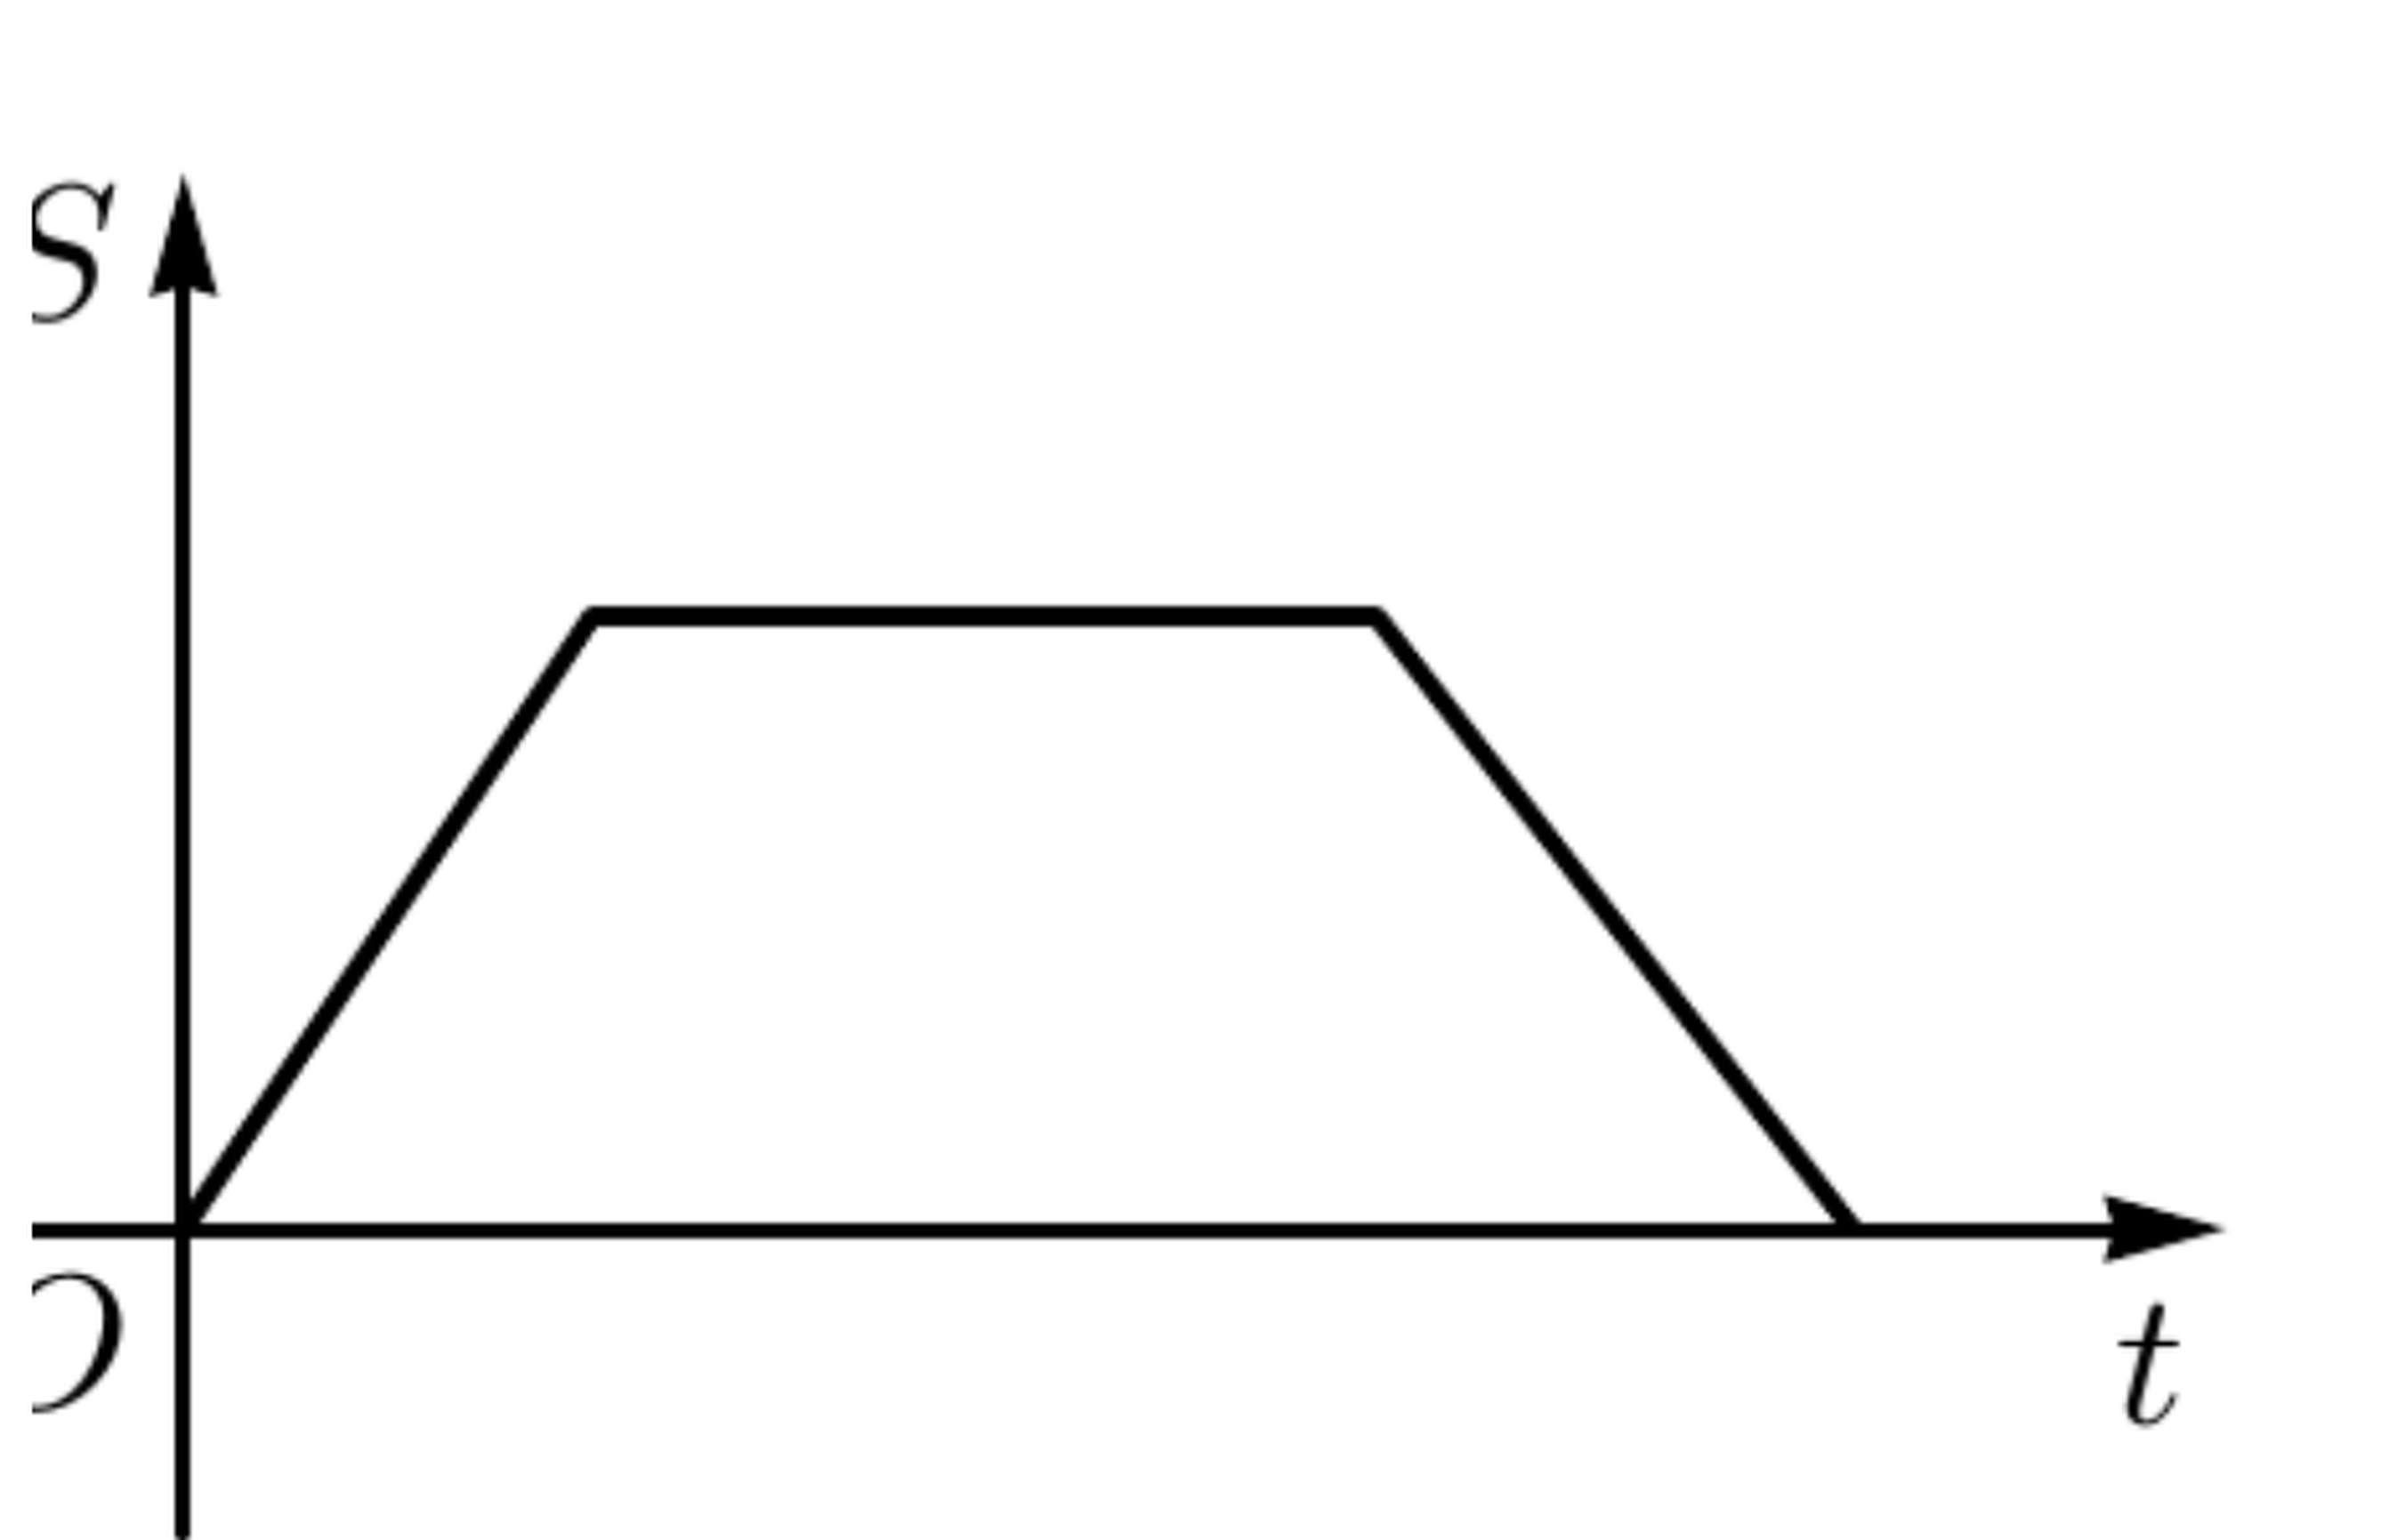
\includegraphics[width=0.34\textwidth]{figures/gao156_q14_st.png}
\end{center}

\keepwithprev
\begin{center}
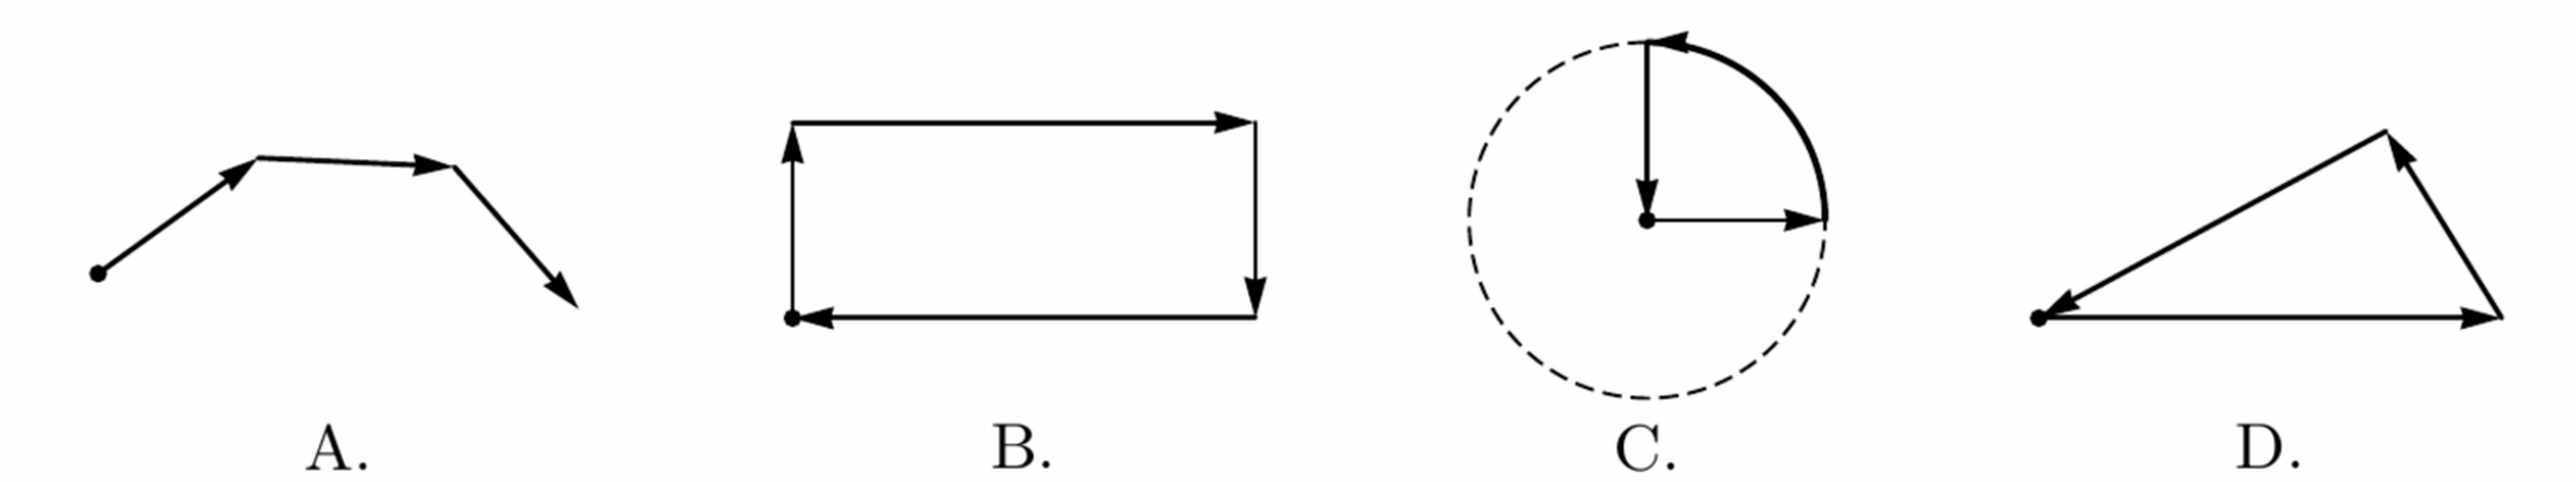
\includegraphics[width=0.86\textwidth]{figures/gao156_q14_opts.png}
\end{center}

\ifanswer
\solbegin
\step{由王老师锻炼时所走的离家距离（$S$）与行走时间（$t$）之间的函数关系图，}
\step{得在中间一段时间里，他到家的距离为定值，}
\step{故他所走的路程是一段以家为圆心的圆弧，故选 $C$.}
\solend
\fi

% === Q15 === 解析内曲线交点图（仅答案版出）；解析 4 行，故选 B
\item 已知 $a+2^a=b+\log_2 b=c+\log_3 c=k$，若 $k<1$，则\mbox{（\quad）}

\keepwithprev
A. $c<a<b$\qquad B. $a<c<b$\qquad C. $b<a<c$\qquad D. $a<b<c$

\ifanswer
\solbegin
\step{因为 $a+2^a=b+\log_2 b=c+\log_3 c=k$，}
\step{所以 $2^a=-a+k$，$\log_2 b=-b+k$，$\log_3 c=-c+k$，其中 $k<1$；}
\step{分别作出 $y=2^x$，$y=\log_2 x$，$y=\log_3 x$ 和 $y=-x+k$ 的图象，}

\begin{center}
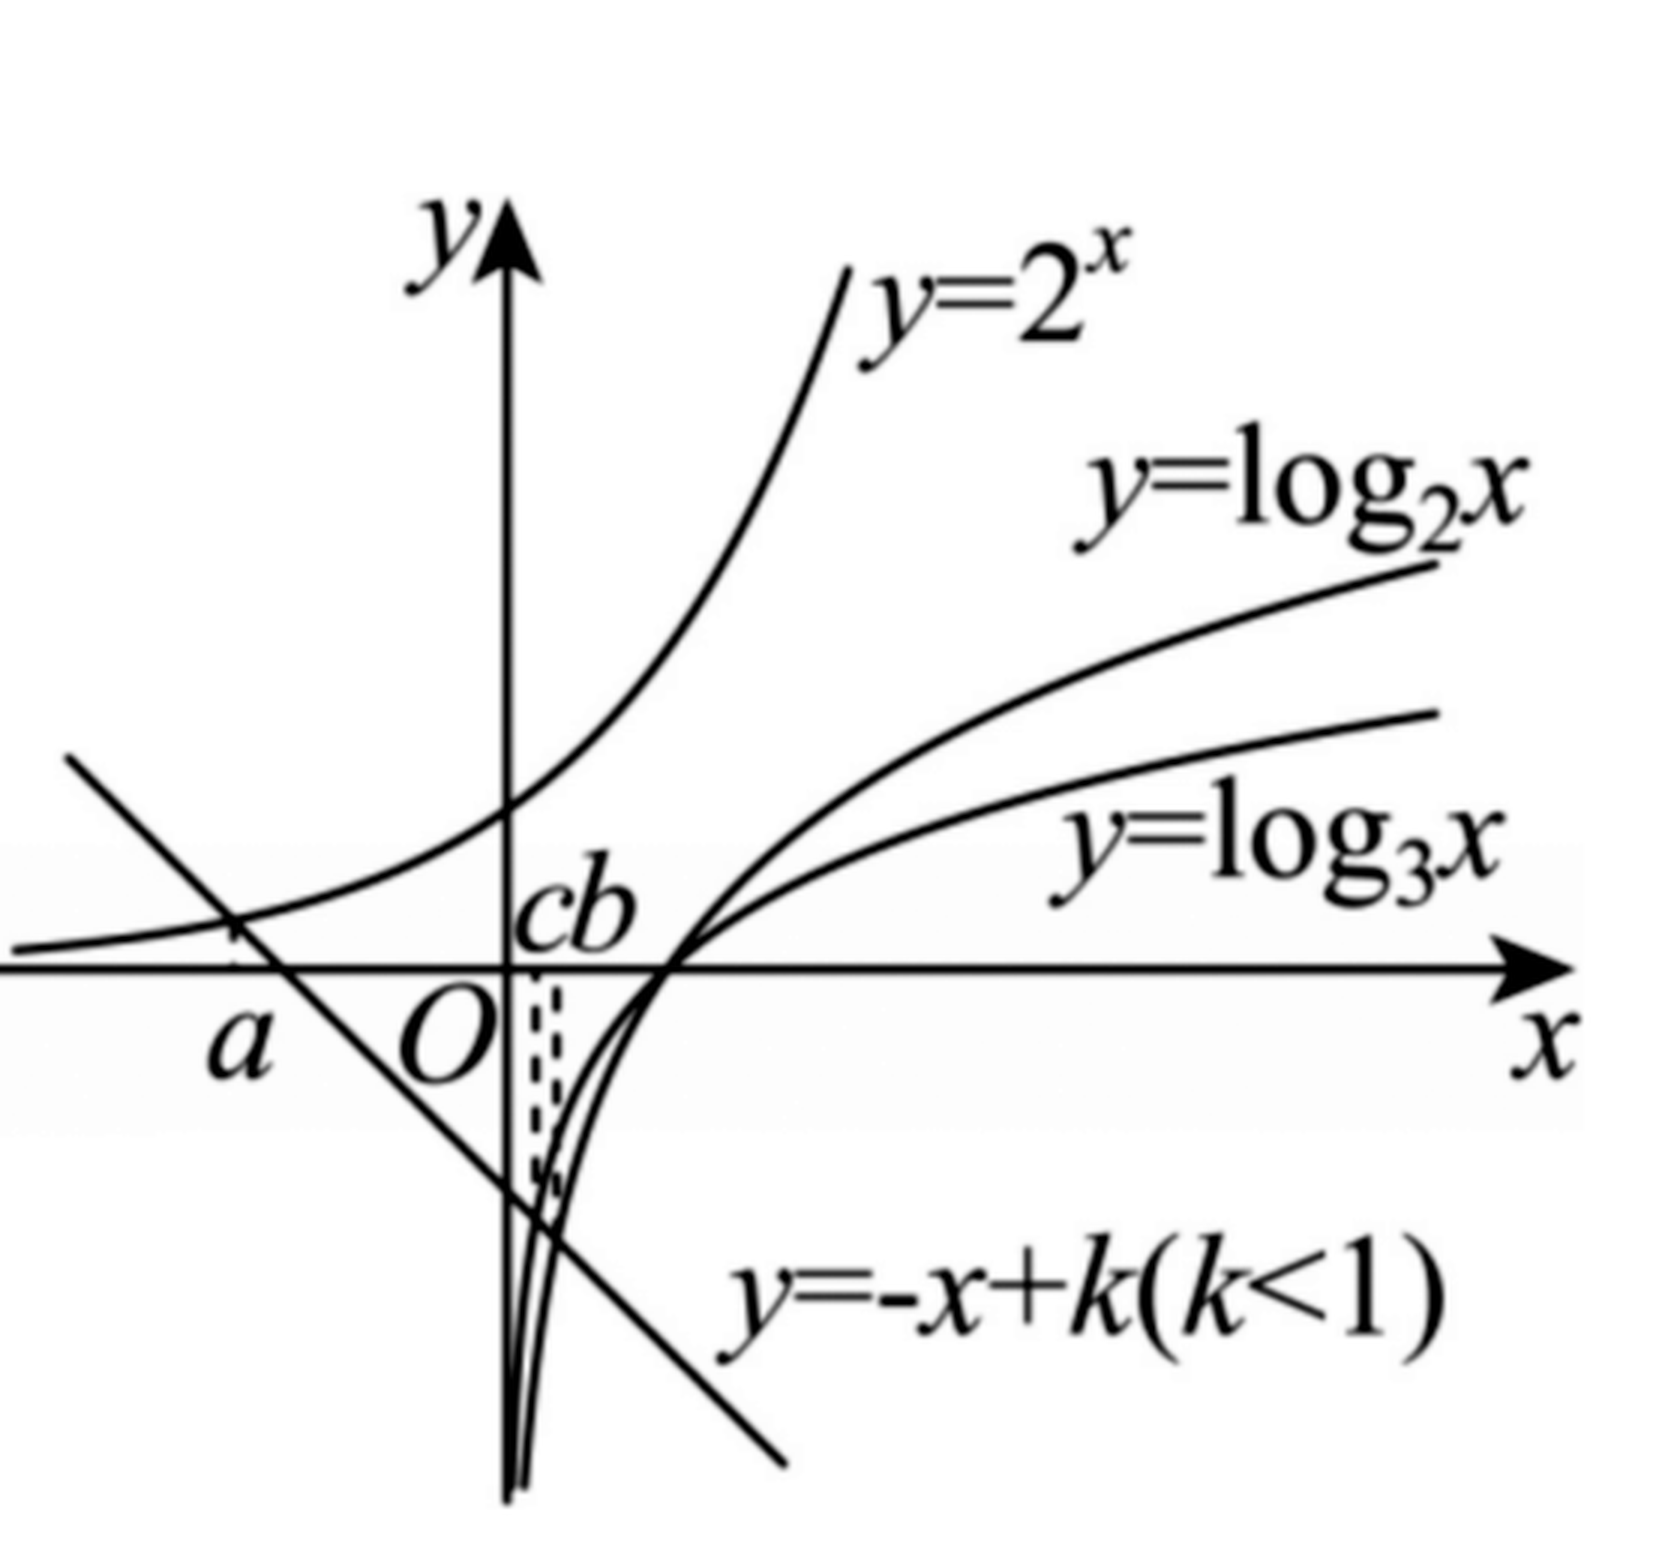
\includegraphics[width=0.52\textwidth]{figures/gao156_q15_curves.png}
\end{center}

\step{如图所示，由图象得 $a<c<b$. 故选 $B$.}
\solend
\fi

% === Q16 === ①② 文本圈数字、"一阶/二阶不动点""稳定点"自定义名词；解析 5 行，故选 A
\item 对定义域为 $I$ 的函数 $y=f(x)$，若存在 $x_0\in I$ 使得 $f(x_0)=x_0$，则称 $x_0$ 是函数 $f(x)$ 的
一阶不动点，简称不动点；若存在 $x_0\in I$ 使得 $f(f(x_0))=x_0$，则称 $x_0$ 是函数 $f(x)$ 的二阶
不动点，简称稳定点. 现有如下两个命题：①存在函数非 $y=x$ 且有无穷多个不动点；②
存在函数有无穷多个稳定点，且这些稳定点不都是不动点. 则\mbox{（\quad）}

\keepwithprev
A. ①成立，②成立\qquad\qquad B. ①成立，②不成立

C. ①不成立，②成立\qquad\qquad D. ①不成立，②不成立

\ifanswer
\solbegin
\step{①取定义在全体实数上的 $f(x)=\lvert x\rvert$，其不动点为一切非负实数，有无穷多个，}
\step{且 $f(-1)=1\ne-1$，①成立.}
\step{②取定义在全体实数上的 $g(x)=-x$，则 $g(g(x))=-(-x)=x$，}
\step{全体实数都是稳定点，而不动点只有 0，②成立.}
\step{故选 $A$.}
\solend
\fi

\end{enumerate}

\bigsec{三、解答题}

\begin{enumerate}
\setcounter{enumi}{16}

% === Q17 === $A\cap B$、$B\cap C$、\varnothing、\mid；解析 6 行
\item 设集合 $A=\{x\mid-1\leqslant x\leqslant2\}$，$B=\{x\mid2m<x<1\}$，$C=\{x\mid x<-1$ 或 $x>2\}$.

(1) 若 $A\cap B=B$，求实数 $m$ 的取值范围；

(2) 若 $B\cap C$ 中只有一个整数，求实数 $m$ 的取值范围.

\ifanswer
\solbegin
\step{(1) 当 $m\geqslant\dfrac12$ 时，$B=\varnothing$，满足 $A\cap B=B$.}
\step{当 $m<\dfrac12$ 时，$A\cap B=B$ 等价于 $2m\geqslant-1$，得 $-\dfrac12\leqslant m<\dfrac12$.}
\step{因此 $m$ 的取值范围为 $\left[-\dfrac12,+\infty\right)$.}
\step{(2) $B\cap C=\{x\mid2m<x<-1\}$，其中只有一个整数时，该整数必为 $-2$.}
\step{包含 $-2$ 且不包含 $-3$，等价于 $-3\leqslant2m<-2$，}
\step{因此 $m$ 的取值范围为 $\left[-\dfrac32,-1\right)$.}
\solend
\fi

% === Q18 === 幂函数 $x^{-\frac13}$、$m\in\R$；解析 12 行，跨 05—06 页
\item 已知幂函数 $f(x)=(3m^2-2m)x^m$（$m\in\R$）在定义域上不单调.

(1) 求函数 $f(x)$ 的解析式；

(2) 若 $f(a+1)<f(-2a+3)$，求实数 $a$ 的取值范围.

\ifanswer
\solbegin
\step{(1) 由幂函数的定义，$3m^2-2m=1$，即 $(3m+1)(m-1)=0$，得 $m=1$ 或 $m=-\dfrac13$.}
\step{当 $m=1$ 时，$f(x)=x$ 在定义域上单调递增，不合题意.}
\step{当 $m=-\dfrac13$ 时，$f(-1)=-1<f(1)=1$，而 $f(1)=1>f(8)=\dfrac12$，}
\step{故 $f(x)$ 在定义域上不单调.}
\step{因此 $f(x)=x^{-\frac13}$，定义域为 $(-\infty,0)\cup(0,+\infty)$.}
\step{(2) 有意义的条件为 $a\ne-1$ 且 $a\ne\dfrac32$.}
\step{当 $a<-1$ 时，$a+1<0<-2a+3$，有 $f(a+1)<0<f(-2a+3)$，}
\step{不等式成立.}
\step{当 $-1<a<\dfrac32$ 时，利用 $f(x)$ 在 $(0,+\infty)$ 上单调递减，}
\step{原不等式等价于 $a+1>-2a+3$，得 $\dfrac23<a<\dfrac32$.}
\step{当 $a>\dfrac32$ 时，$f(a+1)>0>f(-2a+3)$，不等式不成立.}
\step{所以 $a\in(-\infty,-1)\cup\left(\dfrac23,\dfrac32\right)$.}
\solend
\fi

% === Q19 === 两套解法（法一红字 \stepm，法二无标签）；\Delta 与 \subseteq；解析 21 行，跨 06—08 页
\item 已知 $a,c\in\R$，函数 $f(x)=\dfrac{x^2+(3a+1)x+c}{x+a}$.

(1) 若 $a=0$，求函数的定义域，并判断是否存在 $c$ 使得 $y=f(x)$ 图像关于原点对称，说明理由；

(2) 若函数过点 $(1,3)$，且函数 $y=f(x)$ 与 $x$ 轴负半轴有两个不同交点，求此时 $c$ 的值和 $a$ 的取值范围.

\ifanswer
\solbegin
\step{(1) 当 $a=0$ 时，$f(x)=\dfrac{x^2+(3a+1)x+c}{x+a}=\dfrac{x^2+x+c}{x}=x+\dfrac cx+1$，}
\step{故定义域为 $(-\infty,0)\cup(0,+\infty)$；}
\step{若存在实数 $c$，使得函数 $f(x)$ 为奇函数，则必有 $f(x)+f(-x)=0$，}
\step{而 $x+\dfrac cx+1+(-x)+\dfrac c{-x}+1=2\ne0$，}
\step{所以不存在实数 $c$，使得函数 $f(x)$ 为奇函数；}
\step{(2) 函数 $f(x)$ 的图像过点 $(1,3)$，则 $f(1)=\dfrac{1+(3a+1)+c}{1+a}=\dfrac{3a+c+2}{a+1}=3$，}
\step{解得 $c=1$，所以 $f(x)=\dfrac{x^2+(3a+1)x+1}{x+a}$，}
\stepm{法一：}{令 $f(x)=0$，则 $x^2+(3a+1)x+1=0$，此时方程有两不等负根，}
\step{则有 $\begin{cases}\Delta=(3a+1)^2-4>0\\-(3a+1)<0\end{cases}\Rightarrow\begin{cases}a>\dfrac13\text{ 或 }a<-1\\a>-\dfrac13\end{cases}\Rightarrow a>\dfrac13$，}
\step{注意到分母 $x+a\ne0$，则 $x\ne-a$，}
\step{若 $x=-a$ 也是方程 $x^2+(3a+1)x+1=0$ 的解，}
\step{代入方程 $(-a)^2+(3a+1)(-a)+1=0\Rightarrow2a^2+a-1=(a+1)(2a-1)=0$，}
\step{解得 $a=-1$ 或 $a=\dfrac12$，从而 $a\ne\dfrac12$，}
\step{综上，实数 $a$ 的取值范围为 $\left(\dfrac13,\dfrac12\right)\cup\left(\dfrac12,+\infty\right)$.}
\step{令 $g(x)=x^2+(3a+1)x+1$，与 $x$ 轴负半轴有两个交点，}
\step{则 $\begin{cases}-(3a+1)<0\\\Delta=(3a+1)^2-4>0\end{cases}\Rightarrow a>\dfrac13$.}
\step{注意到分母 $x+a\ne0$，则 $x\ne-a$，}
\step{若 $x=-a$ 也是方程 $x^2+(3a+1)x+1=0$ 的解，}
\step{代入方程 $(-a)^2+(3a+1)(-a)+1=0\Rightarrow2a^2+a-1=(a+1)(2a-1)=0$，}
\step{解得 $a=-1$ 或 $a=\dfrac12$，从而 $a\ne\dfrac12$，}
\step{综上，实数 $a$ 的取值范围为 $\left(\dfrac13,\dfrac12\right)\cup\left(\dfrac12,+\infty\right)$.}
\solend
\fi

% === Q20 === $Q$ 常数段 80000 照录；cases 与基本不等式；解析 10 行，跨 08—09 页
\item 某工厂生产某种零件的固定成本为 20000 元，每生产一个零件要增加投入 100 元，已知
总收入 $Q$（单位：元）关于产量 $x$（单位：个）满足函数：$Q=\begin{cases}400x-\dfrac12x^2,&0\leqslant x\leqslant400\\80000,&x>400\end{cases}$.

(1) 将利润 $P$（单位：元）表示为产量 $x$ 的函数；（总收入$=$总成本$+$利润）

(2) 当产量为何值时，零件的单位利润最大？最大单位利润是多少元？（单位利润$=$利润$\div$产量）

\ifanswer
\solbegin
\step{(1) 当 $0\leqslant x\leqslant400$ 时，}
\step{$P(x)=400x-\dfrac12x^2-20000-100x=-\dfrac12x^2+300x-20000$，}
\step{当 $x>400$ 时，$P(x)=80000-100x-20000=60000-100x$，}
\step{故 $P(x)=\begin{cases}-\dfrac12x^2+300x-20000,&0\leqslant x\leqslant400\\60000-100x,&x>400\end{cases}$.}
\step{(2) 设零件的单位利润为 $g(x)$，则 $g(x)=\begin{cases}-\dfrac12x-\dfrac{20000}{x}+300,&0\leqslant x\leqslant400\\\dfrac{60000}{x}-100,&x>400\end{cases}$，}
\step{当 $0\leqslant x\leqslant400$ 时，}
\step{$g(x)=300-\left(\dfrac12x+\dfrac{20000}{x}\right)\leqslant300-2\sqrt{\dfrac x2\cdot\dfrac{20000}{x}}=100$，}
\step{当且仅当 $\dfrac x2=\dfrac{20000}{x}$，即 $x=200$ 时取等号，}
\step{当 $x>400$ 时，$g(x)=\dfrac{60000}{x}-100$，此时无最值，}
\step{故当产量为 200 个，零件的单位利润最大，最大单位利润是 100 元.}
\solend
\fi

% === Q21 === 上升集定义、$D(x_0)=\{d\in\R\mid\cdots\}$、①②③ 文本圈数字、
%            \subseteq 带下划线、$-2^{-x}$；解析 19 行，跨 09—10 页
\item 已知函数 $y=f(x)$ 的定义域为 $\R$. 对任意 $x_0\in\R$，定义集合
$D(x_0)=\{d\in\R\mid f(x_0+d)>f(x_0)\}$，则称 $D(x_0)$ 为函数 $y=f(x)$ 在 $x_0$ 处的上升集.

(1) 若 $f(x)=1-x$，求 $D(-1)$；

(2) 若 $f(x)=\begin{cases}2^x,&x<0\\0,&x=0\\-2^{-x},&x>0\end{cases}$，求 $D(x)$；

(3) 设 $y=f(x)$ 满足：①当 $x<0$ 时，$f(x)=2^x$；②若 $f(x_1)\leqslant f(x_2)$，则
$D(x_2)\subseteq D(x_1)$；③当 $0<x<1$ 时，$f(x)<f(0)$. 证明：$f(0)\geqslant1$.

\ifanswer
\solbegin
\step{(1) $f(-1+d)>f(-1)\Leftrightarrow2-d>2\Leftrightarrow d<0$，所以 $D(-1)=(-\infty,0)$.}
\step{(2) 函数在 $(-\infty,0)$、$(0,+\infty)$ 上分别严格递增，}
\step{且这两个区间上的函数值分别为正、负，$f(0)=0$.}
\step{当 $x<0$ 时，$f(x+d)>f(x)\Leftrightarrow x<x+d<0\Leftrightarrow0<d<-x$，}
\step{当 $x=0$ 时，$f(d)>f(0)\Leftrightarrow d<0$，}
\step{当 $x>0$ 时，$f(x+d)>f(x)\Leftrightarrow x+d\leqslant0$ 或 $x+d>x$}
\step{$\Leftrightarrow d\leqslant-x$ 或 $d>0$，}
\step{因此 $D(x)=\begin{cases}(0,-x),&x<0\\(-\infty,0),&x=0\\(-\infty,-x]\cup(0,+\infty),&x>0\end{cases}$.}
\step{(3) 任取 $a\in(-1,0)$，}
\step{令 $d=-\dfrac a2$，则 $0<d<1$，且 $f(a+d)=2^{\frac a2}>2^a=f(a)$，}
\step{所以 $d\in D(a)$；}
\step{由③，$f(d)<f(0)$，所以 $d\notin D(0)$.}
\step{若 $f(0)\leqslant f(a)$，由②得 $D(a)\subseteq D(0)$，与上述结论矛盾.}
\step{因此，对任意 $a\in(-1,0)$，都有 $f(0)>2^a$.}
\step{特别地 $f(0)>2^{-\frac12}>0$.}
\step{若 $f(0)<1$，取 $a=\dfrac12\log_2 f(0)$，则 $-\dfrac14<a<0$，且}
\step{$2^a=\sqrt{f(0)}>f(0)$，}
\step{与 $f(0)>2^a$ 矛盾.}
\step{所以 $f(0)\geqslant1$.}
\solend
\fi

\end{enumerate}

\end{document}
"
% 紧凑版：xelatex "\def\iscompact{1}% 高一156_大同中学_期中.tex
%   —— 高一上数学"2026-2027 年大同中学高一上期中"（试卷版/答案版/紧凑版）
% 试卷版：xelatex 高一156_大同中学_期中.tex
% 答案版：xelatex "\def\isanswer{1}\input{高一156_大同中学_期中.tex}"
% 紧凑版：xelatex "\def\iscompact{1}\input{高一156_大同中学_期中.tex}"
%
% ① 原始材料：微信公众号"魔都数学加油站"文章，连载"27学年高一156"，原文标题
% "27学年高一156——2026-2027年上海市大同中学高一上期中"；
% 原文链接：https://mp.weixin.qq.com/s/xLtS5tyjCPJIWCIBohwGvw 。
% 正文为 10 张 PNG 页（01/02/03/04/05/06/07/08/09/10 各页分辨率混排
% 2560×3620 与 4762×6735，逐页按各自分辨率裁图核对）。
% 体例：讲评版——填空 3—12（10 题）、选择 13—16（4 题）、解答 17—21（5 题），
% 共 19 题，自第 3 题起编（1、2 未印在本篇）；Q3 只印【答案】、其余 18 题
% 逐题印【解析】（逐题核实，见 ②）。题目、答案、解析均据原图转录；卷面粉红色
% 水印"魔都数学加油站"及公众号页脚未录入。
%
% 卷首标题：原卷印作"2026-2027 年大同中学高一上期中"，年份区间按全稿惯例排 en dash；
% 原卷卷面未印副标题，本稿按同期中卷知识模块口径补出"集合与常用逻辑用语、不等式、函数"。
%
% ② 与原卷的排版差异：
%   ① 原文从第 3 题起，本稿保留原题号；共 19 题三节，解答题 5 题到 21；
%   ② 混合体例：第 3 题只印【答案】、无【解析】，按 高一140 第 5 题／高一145
%      第 3 题／高一151 第 7 题成例另提 \ans{}、不补造解析；其余 18 题印
%      【解析】、用 \solbegin…\solend；四道选择题答案在解析末句"故选 C／C／B／A"
%      （逐个放大复核）、括号 \mbox{（\quad）} 留空、不另提 \ans{}；答案版
%      【答案】/【解析】标记数 = 19 = 全卷题数（1 个 \ans ＋ 18 个 \solbegin）；
%   ③ 原卷卷面未印副标题，本稿按知识模块口径补出；
%   ④ 原卷填空横线按全稿惯例排 \blankline[4.4em]；选择题括号排 \mbox{（\quad）}、
%      选项段前按惯例各加 \keepwithprev；解答题不留作答区、不加 \anspace
%      （原卷为讲评版，109—113 起全稿不用 \anspace）；
%   ⑤ 数集：Q3"$x\in\R$"、Q18"$m\in\R$"、Q19"$a,c\in\R$"、Q21"定义域为 \R"
%      "任意 $x_0\in\R$""$d\in\R$"原卷印正体粗体 R，按全稿惯例归一 \R；
%      绝对值排 \lvert…\rvert（Q11 $\lvert2^x-1\rvert$、Q16 $\lvert x\rvert$），
%      集合描述竖线排 \mid（Q17 $A=\{x\mid\cdots\}$、Q21 $D(x_0)=\{d\in\R\mid\cdots\}$），
%      空集 \varnothing（Q17"$B=\varnothing$"），不等号按全稿惯例排 \leqslant／\geqslant；
%   ⑥ 子集符号逐处照录不统一：Q21 (3) 题干"$D(x_2)\subseteq D(x_1)$"与解析
%      "$D(a)\subseteq D(0)$"均印带下划线 ⊆，照录 \subseteq；本卷无单线 ⊂ 用例；
%   ⑦ 判别式：Q19 两套解法"$\Delta=(3a+1)^2-4>0$"印等腰偏高 \Delta，照录 \Delta；
%      本卷无扁三角 \triangle 用例；
%   ⑧ 红字照录为黑体：Q19 (2) 解析第一套解法行首"法一："原卷排**红色加粗**，
%      按 高一53 成例排 \stepm{法一：}{…}（加粗着色、不改黑色基调），全库无红字
%      排字先例、本稿不引入红色定义，文件头注明；第二套解法原卷直接以
%      "令 $g(x)=x^2+(3a+1)x+1$，与 $x$ 轴负半轴有两个交点，"另起，
%      **未印"法二："标签**（逐页像素级复核：07 页仅 1437—1475 一处红字，
%      08 页无红字），照录为普通 \step、不补造标签；
%   ⑨ 文本模式圈数字逐处照录：Q12 解析 ①② 两情形、Q16 两则命题与四个选项及
%      解析的 ①②、Q21 (3) 三条件 ①②③ 与解析"由③""由②"，均为印刷圈数字
%      （非 \textcircled、非数学模式），计入圈数字实测；
%   ⑩ 自定义名词照录：Q16"一阶不动点，简称不动点""二阶不动点，简称稳定点"、
%      Q21"上升集"；Q16 题干"存在函数非 $y=x$ 且有无穷多个不动点"照录；
%   ⑪ 中文弯引号照录：Q3""存在 $x\in\R$，$x^3-1\leqslant0$" 否定形式为"、
%      Q13"使"$\dfrac{x+1}{1-x}\geqslant0$"成立的必要不充分条件是"；
%      注释里一律 ASCII 引号；数学式内 CJK 用 \text{}（Q19 cases 内"或"）；
%   ⑫ 半角逗号在数学组之间是全稿惯例、非笔误，逐处照录（$a,c$、$x,y$、$a,b$
%      之类）；行末西文句点 ASCII `.`；行中全角逗号／顿号照录；
%   ⑬ 复杂式照录别简化：Q6 $\left(\dfrac{1}{\sqrt a}\right)^{\frac27}\cdot\sqrt[7]{a^3}$
%      与解析 $a^{\frac{12}{7}-\frac17+\frac37}$、Q8 $2\sqrt4+5=9$（$\sqrt4$ 未化简）、
%      Q9 $\left(\sqrt x+\dfrac{1}{\sqrt x}\right)^3$、Q12 $\dfrac{4a-(2-a)^2}{4a}$、
%      Q18 $f(8)=\dfrac12$、Q19 $2a^2+a-1=(a+1)(2a-1)=0$、Q20 $Q$ 的常数段
%      $80000$（不是 $80000-100x$）与 $2\sqrt{\dfrac x2\cdot\dfrac{20000}{x}}$、
%      Q21 $f(a+d)=2^{\frac a2}>2^a=f(a)$ 与 $2^a=\sqrt{f(0)}>f(0)$ 等；
%      \left…\right 不得拆到不同 $…$ 组（Q5 $\left(0,\dfrac12\right)$、
%      Q12 $\left[0,4+2\sqrt3\right)$、Q17 $\left[-\dfrac12,+\infty\right)$、
%      Q19 $\left(\dfrac13,\dfrac12\right)\cup\left(\dfrac12,+\infty\right)$、
%      Q20 $\left(\dfrac12x+\dfrac{20000}{x}\right)$ 等）；cases 块整体算一个印刷行；
%   ⑭ 一条 \step = 原卷解析的一个印刷行；别并折行、别拆行。跨页续印按题合并
%      （Q6 的 01 页上下题干重复印、Q8 的 01—02 页、Q12 的 02—03 页、
%      Q15 的 04 页上下、Q16 的 04—05 页、Q17 的 05 页上下、Q18 的 05—06 页、
%      Q19 的 06—08 页、Q20 的 08—09 页、Q21 的 09—10 页）；
%      跨半页重叠行（Q12 的"②若 …"、Q18 的"原不等式等价于 …"、
%      Q20 的"【解析】(1) 当 $0\leqslant x\leqslant400$ 时，"、Q21 的
%      "【解析】(1) $f(-1+d)>f(-1)\cdots$"与"与 $f(0)>2^a$ 矛盾."）
%      只算一个印刷行；
%   ⑮ 配图：全卷 3 组（逐页通读 10 页确认）——
%      · Q14 题干 S-t 梯形图（03 页右下，离家距离 S 对行走时间 t），题目配图、
%        三版都出，裁 figures/gao156_q14_st.png；
%      · Q14 四幅路线选项（04 页上部，A/B/C/D 四幅横排、C 为以家为圆心的圆弧），
%        题目配图、三版都出，合并成一张，裁 figures/gao156_q14_opts.png；
%      · Q15 解析内曲线交点图（04 页右下，$y=2^x$、$y=\log_2x$、$y=\log_3x$
%        与 $y=-x+k$），仅答案版出，裁 figures/gao156_q15_curves.png；
%      3 图均取自原卷截图，去粉色水印、去色、3×~4× LANCZOS 放大；
%      Q14 题干"题干＋两图"整块用 \needvspace 守卫推走（守卫放 \item 之前，
%      见 高一154 Q15／高一136 Q13 成例）；Q15 解析内图放 \ifanswer 内
%      \solbegin…\solend 的两 \step 之间（高一108 第 6 题／高一154 附加题 2 成例）；
%      其余各页逐页确认无其它题目配图、无解析配图、无表格；10 页下半仅水印、无正文。
%
% ③ 行数复核：一条 \step = 原卷解析的一个印刷行，cases 块作一个印刷行计。
%   逐题数（主会话逐页核对定稿）：Q3：0（只印【答案】、提 \ans{}，不计入 \step 账）；
%   Q4：1；Q5：1；Q6：1；Q7：1；Q8：3；Q9：2；Q10：2；Q11：5；Q12：12；
%   Q13：3；Q14：3；Q15：4；Q16：5；Q17：6；Q18：12；Q19：21；Q20：10；Q21：19。
%   合计 111 行（110 条 \step ＋ 1 条 \stepm），与原卷逐题印刷行相等。
%   全卷 19 题：Q3 一处 \ans{} ＋ 其余 18 题设 \solbegin…\solend，
%   答案版【答案】/【解析】标记数 = 19 = 全卷题数。
%
% ④ 页码分布（供回原图复核）：
%   卷首标题＋"一、填空题"＋Q3 题干＋【答案】、Q4 题干＋解析 1 行、
%   Q5 题干＋解析 1 行、Q6 题干首行在 01 页上半；
%   Q6 题干（重复印）＋解析 1 行、Q7 题干＋解析 1 行、Q8 题干＋解析前 2 行
%   在 01 页下半；Q8 解析末行、Q9 题干＋解析 2 行、Q10 题干＋解析 2 行、
%   Q11 题干首行在 02 页上半；Q11 题干（重复印）＋解析 5 行、
%   Q12 题干＋解析首行在 02 页下半；Q12 解析中 9 行在 03 页上半；
%   Q12 解析末 2 行＋"二、选择题"标题＋Q13 题干＋选项＋解析 3 行＋
%   Q14 题干首行在 03 页下半；Q14 题干续行＋四幅选项图＋解析 3 行＋
%   Q15 题干＋选项＋解析前 2 行＋Q16 题干在 04 页上半；
%   Q15 解析后 2 行＋曲线图＋Q16 选项＋解析前 2 行在 04 页下半；
%   Q16 解析后 3 行＋"三、解答题"标题＋Q17 题干＋两问＋解析 (1) 3 行
%   在 05 页上半；Q17 解析 (2) 3 行＋Q18 题干＋两问＋解析 (1) 首 2 行
%   在 05 页下半；Q18 解析 (1)(2) 中 8 行在 06 页上半；Q18 解析末 2 行＋
%   Q19 题干＋两问＋解析 (1) 首行在 06 页下半；Q19 解析 (1) 后 4 行＋
%   (2) 前 2 行＋法一 2 行在 07 页上半；法一后 5 行＋法二前 3 行在 07 页下半；
%   法二后 4 行＋Q20 题干＋两问＋解析 (1) 首行在 08 页上半；
%   Q20 解析 (1) 后 3 行＋(2) 前 5 行在 08 页下半；Q20 解析 (2) 末 2 行＋
%   Q21 题干＋三问＋解析 (1) 首行在 09 页上半；Q21 解析 (1)（重复印）＋
%   (2) 8 行＋(3) 首行在 09 页下半；Q21 (3) 解析中 8 行在 10 页上半；
%   Q21 (3) 末 2 行在 10 页下半。本稿按题连排，不丢行、不并折行；
%   全卷末题为第 21 题，无附加题节。
%
\documentclass[a4paper,11pt]{article}
\usepackage{common}

\begin{document}

\examtitlest[3]{2026--2027 年大同中学高一上期中}{集合与常用逻辑用语、不等式、函数}

\bigsec{一、填空题}

\begin{enumerate}
\setcounter{enumi}{2}

% === Q3 === 只印【答案】、无【解析】；R 正体粗体 \R；中文弯引号照录
\item “存在 $x\in\R$，$x^3-1\leqslant0$” 否定形式为\blankline[4.4em].

\ifanswer
\ans{对任意 $x\in\R$，$x^3-1>0$}
\fi

% === Q4 === 解析 1 行
\item 若实数 $a>0$ 且 $a\ne1$，函数 $y=a^{x-3}+1$ 的图像恒过定点 $P$，则点 $P$ 的坐标为\blankline[4.4em].

\ifanswer
\solbegin
\step{当 $x=3$ 时，$y=a^0+1=2$，与 $a$ 无关，所以定点为 $P(3,2)$.}
\solend
\fi

% === Q5 === 解析 1 行
\item 函数 $y=\dfrac{1}{3^x+2}$ 的值域是\blankline[4.4em].

\ifanswer
\solbegin
\step{$3^x\in(0,+\infty)$，因此 $3^x+2\in(2,+\infty)$，值域为 $\left(0,\dfrac12\right)$.}
\solend
\fi

% === Q6 === 根式嵌套照录；解析 1 行；题干跨 01 页上下重复印
\item 已知 $a>0$，化简 $a^{\frac{12}{7}}\cdot\left(\dfrac{1}{\sqrt a}\right)^{\frac27}\cdot\sqrt[7]{a^3}=$\blankline[4.4em].

\ifanswer
\solbegin
\step{原式 $=a^{\frac{12}{7}}\cdot a^{-\frac17}\cdot a^{\frac37}=a^{\frac{12}{7}-\frac17+\frac37}=a^2$.}
\solend
\fi

% === Q7 === 换底公式；解析 1 行
\item 已知 $\log_5 3=a$，用 $a$ 的代数式表示 $\log_{15}125=$\blankline[4.4em].

\ifanswer
\solbegin
\step{$\log_{15}125=\dfrac{\log_5 125}{\log_5 15}=\dfrac{3}{1+\log_5 3}=\dfrac{3}{1+a}$.}
\solend
\fi

% === Q8 === 基本不等式，$\sqrt4$ 照录未化简；解析 3 行，跨 01—02 页
\item 已知 $x>0$，$y>0$，且 $4x+y=xy$，则 $x+y$ 的最小值为\blankline[4.4em].

\ifanswer
\solbegin
\step{由 $4x+y=xy$，得 $\dfrac4y+\dfrac1x=1$，}
\step{则 $x+y=(x+y)\left(\dfrac4y+\dfrac1x\right)=\dfrac{4x}{y}+\dfrac yx+1+4\geqslant2\sqrt4+5=9$，}
\step{当且仅当 $\dfrac{4x}{y}=\dfrac yx$，即 $x=3$，$y=6$ 时取等号，故最小值为 9.}
\solend
\fi

% === Q9 === 解析 2 行
\item 已知 $x^{-1}+x=7$（$x>0$），则 $x^{\frac32}+x^{-\frac32}$ 的值为\blankline[4.4em].

\ifanswer
\solbegin
\step{$x>0$，有 $\sqrt x+\dfrac{1}{\sqrt x}=\sqrt{x+\dfrac1x+2}=3$，}
\step{所以 $x^{\frac32}+x^{-\frac32}=\left(\sqrt x+\dfrac{1}{\sqrt x}\right)^3-3\left(\sqrt x+\dfrac{1}{\sqrt x}\right)=27-9=18$.}
\solend
\fi

% === Q10 === $x_{\min}$；解析 2 行
\item 已知不等式 $x>\dfrac{2a+1}{a-1}$ 对任意的 $x\in[1,2]$ 恒成立，则实数 $a$ 的取值范围是\blankline[4.4em].

\ifanswer
\solbegin
\step{不等式 $x>\dfrac{2a+1}{a-1}$ 对任意的 $x\in[1,2]$ 恒成立，得 $\dfrac{2a+1}{a-1}<x_{\min}=1$，}
\step{即有 $\dfrac{a+2}{a-1}<0$，解得 $-2<a<1$，则实数 $a$ 的取值范围是 $(-2,1)$.}
\solend
\fi

% === Q11 === 分段函数 cases 与绝对值 \lvert…\rvert；解析 5 行
\item 已知函数 $f(x)=\begin{cases}\lvert2^x-1\rvert-a,&x\leqslant2\\\dfrac{3}{x-1}-a,&x>2\end{cases}$，若函数 $y=f(x)$ 图像与 $x$ 轴有三个不同交点，则实数 $a$ 的取值范围是\blankline[4.4em].

\ifanswer
\solbegin
\step{令 $g(x)=f(x)+a$.}
\step{在 $(-\infty,0)$、$[0,2]$、$(2,+\infty)$ 上，$g(x)$ 均严格单调，}
\step{值域依次为 $(0,1)$、$[0,3]$、$(0,3)$.}
\step{每段至多有一个交点，因而恰有三个不同交点，}
\step{当且仅当 $a\in(0,1)\cap[0,3]\cap(0,3)=(0,1)$.}
\solend
\fi

% === Q12 === ①② 文本圈数字、对称轴与最小值式照录；解析 12 行，跨 02—03 页
\item 已知函数 $f(x)=ax^2-(2-a)x+1$，$g(x)=x$，若对于任意实数 $x$，$f(x)$ 与 $g(x)$ 至少有一个为正数，则实数 $a$ 的取值范围是\blankline[4.4em].

\ifanswer
\solbegin
\step{当 $x>0$ 时，$g(x)>0$；当 $x<0$ 时，$g(x)<0$；}
\step{当 $x=0$ 时，$f(0)=1>0$；}
\step{因为对于任意实数 $x$，$f(x)$ 与 $g(x)$ 至少有一个为正数，}
\step{当 $x<0$ 时，因为 $g(x)<0$，所以 $f(x)=ax^2-(2-a)x+1>0$ 恒成立，}
\step{当 $a<0$ 时，显然不成立，}
\step{当 $a=0$ 时，$f(x)=-2x+1>0$，对 $x<0$ 时恒成立，满足题意，}
\step{当 $a>0$ 时，函数图象开口向上，对称轴 $x=\dfrac{2-a}{2a}$，}
\step{①若 $\dfrac{2-a}{2a}\geqslant0$，即 $0<a\leqslant2$ 时，函数 $f(x)$ 在 $(-\infty,0)$ 上严格减，$f(0)=1$，}
\step{故 $f(x)>0$ 对 $x<0$ 时恒成立，满足题意；}
\step{②若 $\dfrac{2-a}{2a}<0$，即 $a>2$ 时，$f(x)_{\min}=f\left(\dfrac{2-a}{2a}\right)=\dfrac{4a-(2-a)^2}{4a}>0$，}
\step{解得 $4-2\sqrt3<a<4+2\sqrt3$，所以 $2<a<4+2\sqrt3$.}
\step{综上，$0\leqslant a<4+2\sqrt3$，故实数 $a$ 的取值范围是 $\left[0,4+2\sqrt3\right)$.}
\solend
\fi

\end{enumerate}

\bigsec{二、选择题}

\begin{enumerate}
\setcounter{enumi}{12}

% === Q13 === 必要不充分条件；cases 块；解析 3 行，故选 C
\item 使 “$\dfrac{x+1}{1-x}\geqslant0$” 成立的必要不充分条件是\mbox{（\quad）}

\keepwithprev
A. $-1\leqslant x<1$\qquad B. $x\leqslant-1$ 或 $x>1$\qquad C. $-1\leqslant x\leqslant1$\qquad D. $x\leqslant-1$ 或 $x\geqslant0$

\ifanswer
\solbegin
\step{由不等式 $\dfrac{x+1}{1-x}\geqslant0$ 得 $\begin{cases}(x+1)(1-x)\geqslant0\\1-x\ne0\end{cases}$，解得 $-1\leqslant x<1$，}
\step{由题意结合选项，$-1\leqslant x<1\Rightarrow-1\leqslant x\leqslant1$ 成立，反之不成立，}
\step{所以 $-1\leqslant x\leqslant1$ 是 $\dfrac{x+1}{1-x}\geqslant0$ 成立的必要不充分条件. 故选 $C$.}
\solend
\fi

% === Q14 === 题干 S-t 图＋四幅路线选项（题目配图，三版都出）；守卫放 \item 之前；解析 3 行，故选 C
\needvspace{9cm}
\item 如图是王老师锻炼时所走的离家距离（$S$）与行走时间（$t$）之间的函数关系图，若
用黑点表示王老师家的位置，则王老师行走的路线可能是\mbox{（\quad）}

\begin{center}
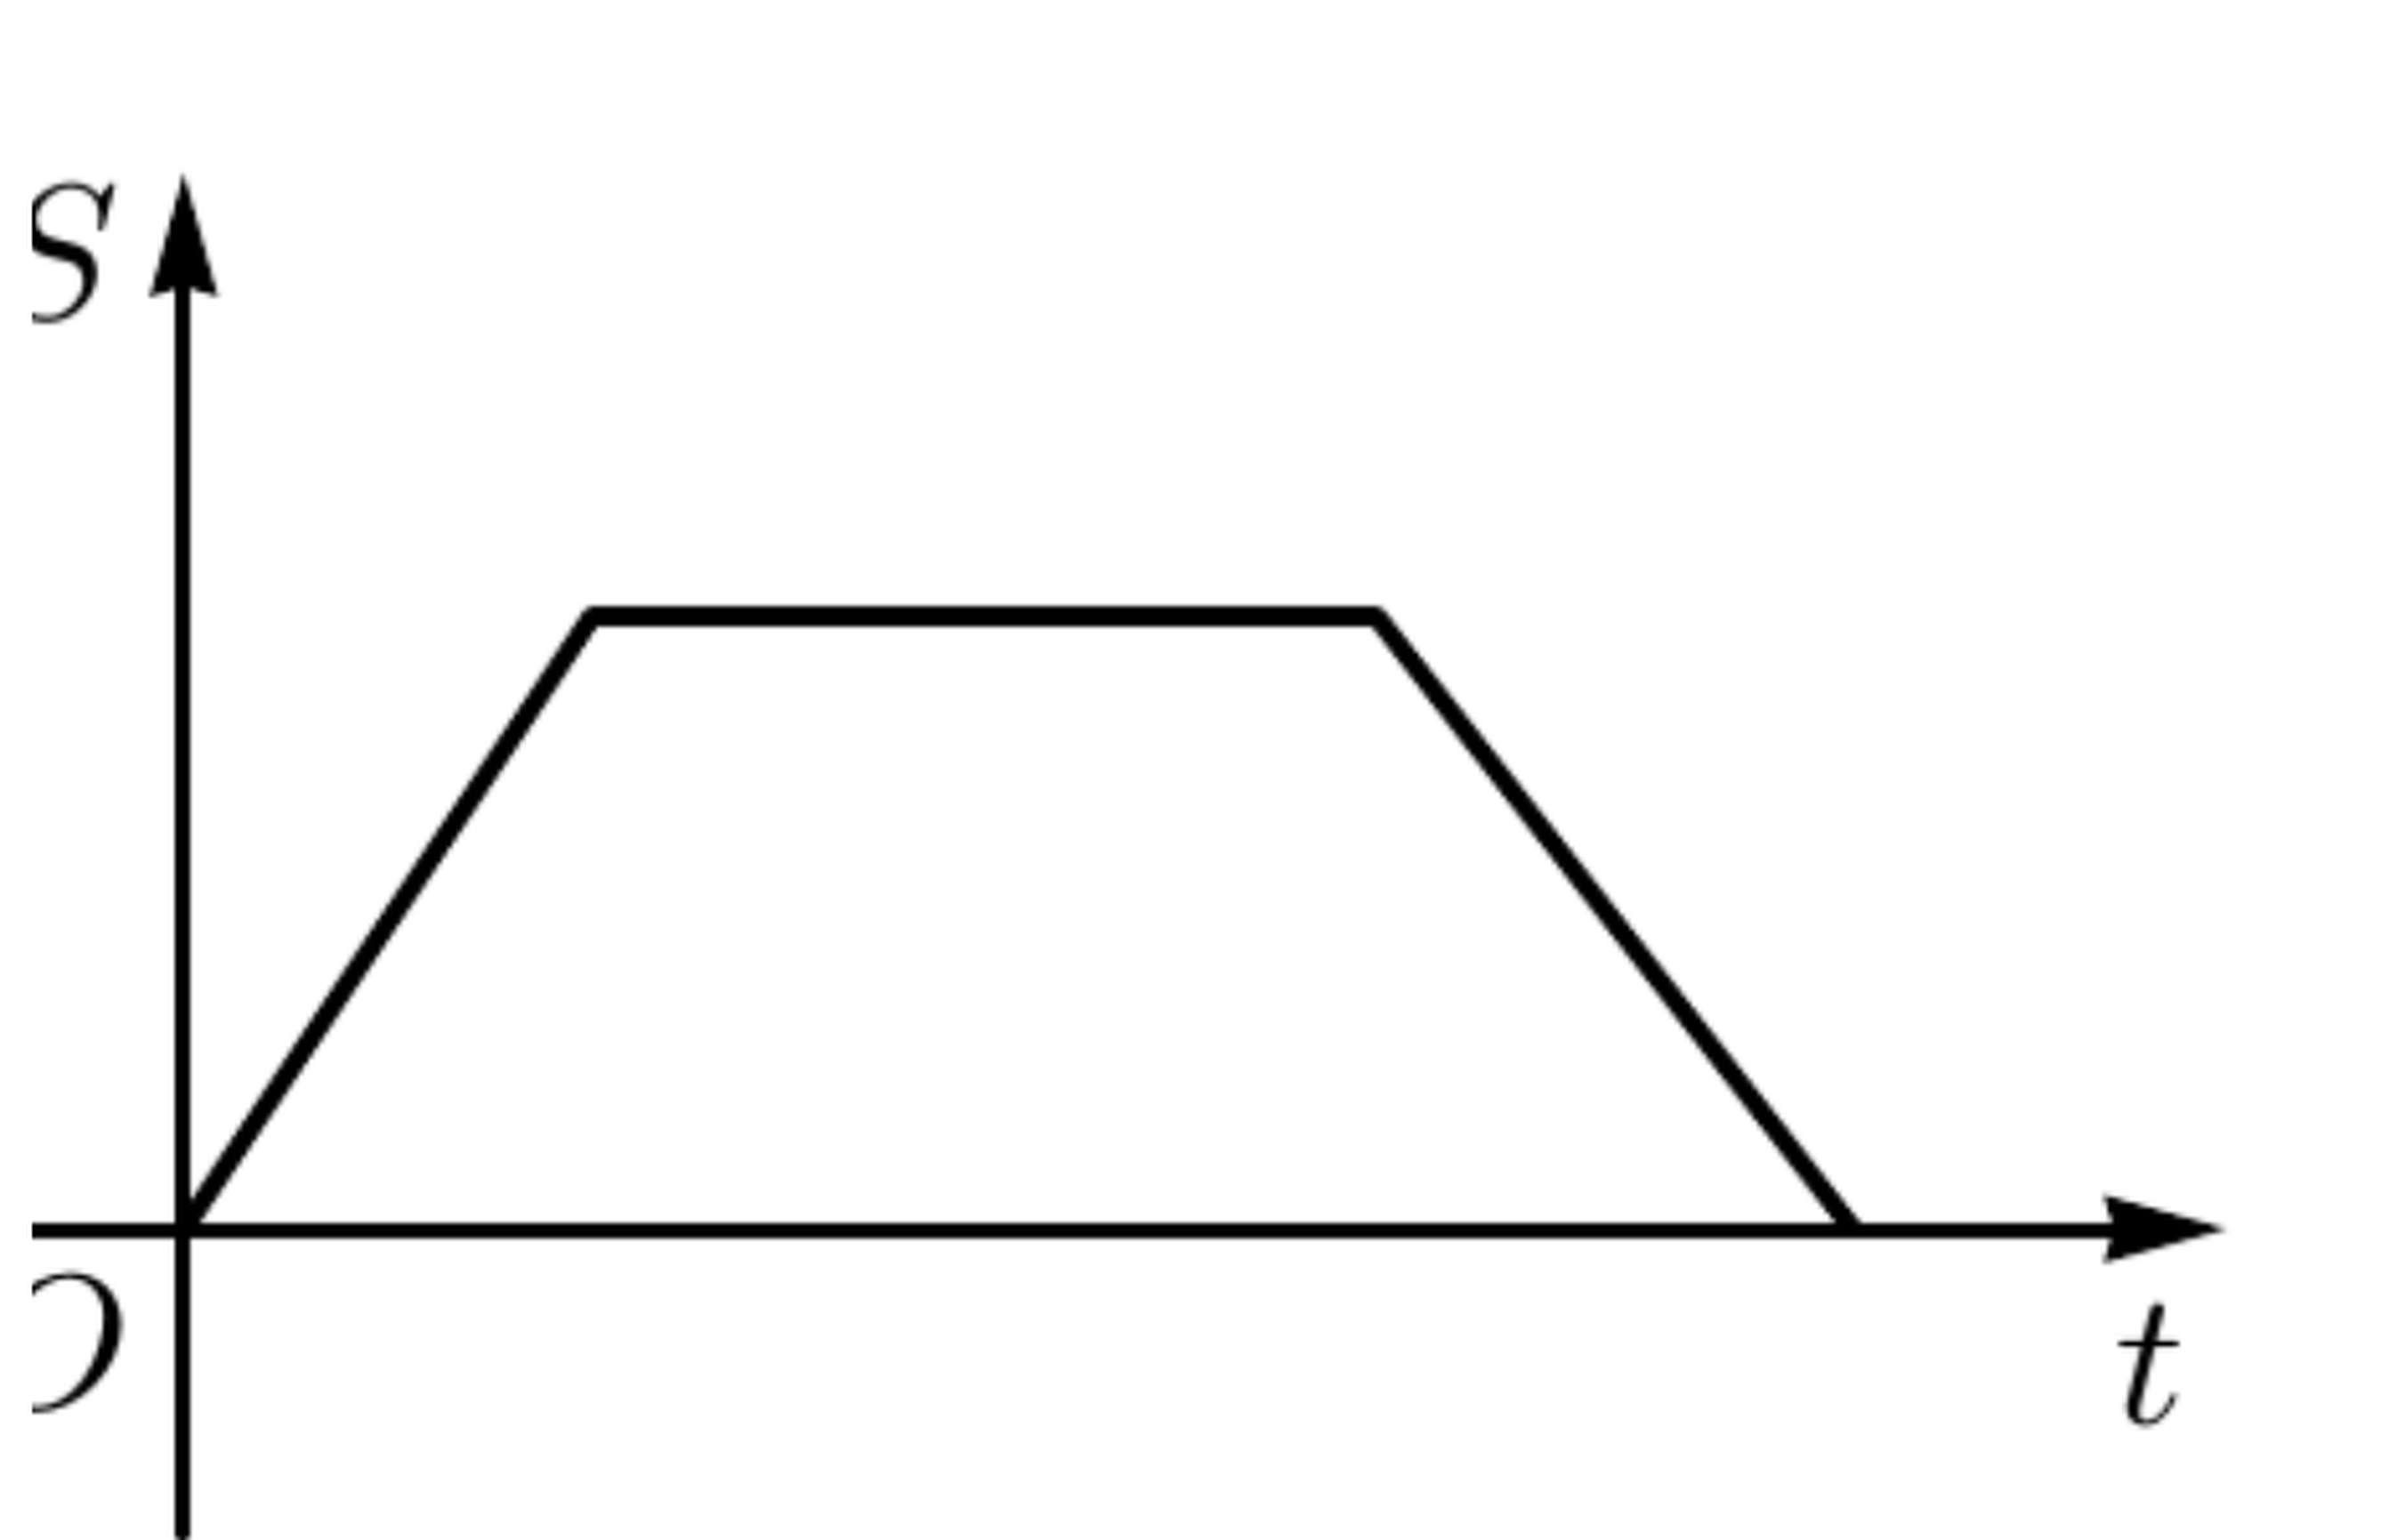
\includegraphics[width=0.34\textwidth]{figures/gao156_q14_st.png}
\end{center}

\keepwithprev
\begin{center}
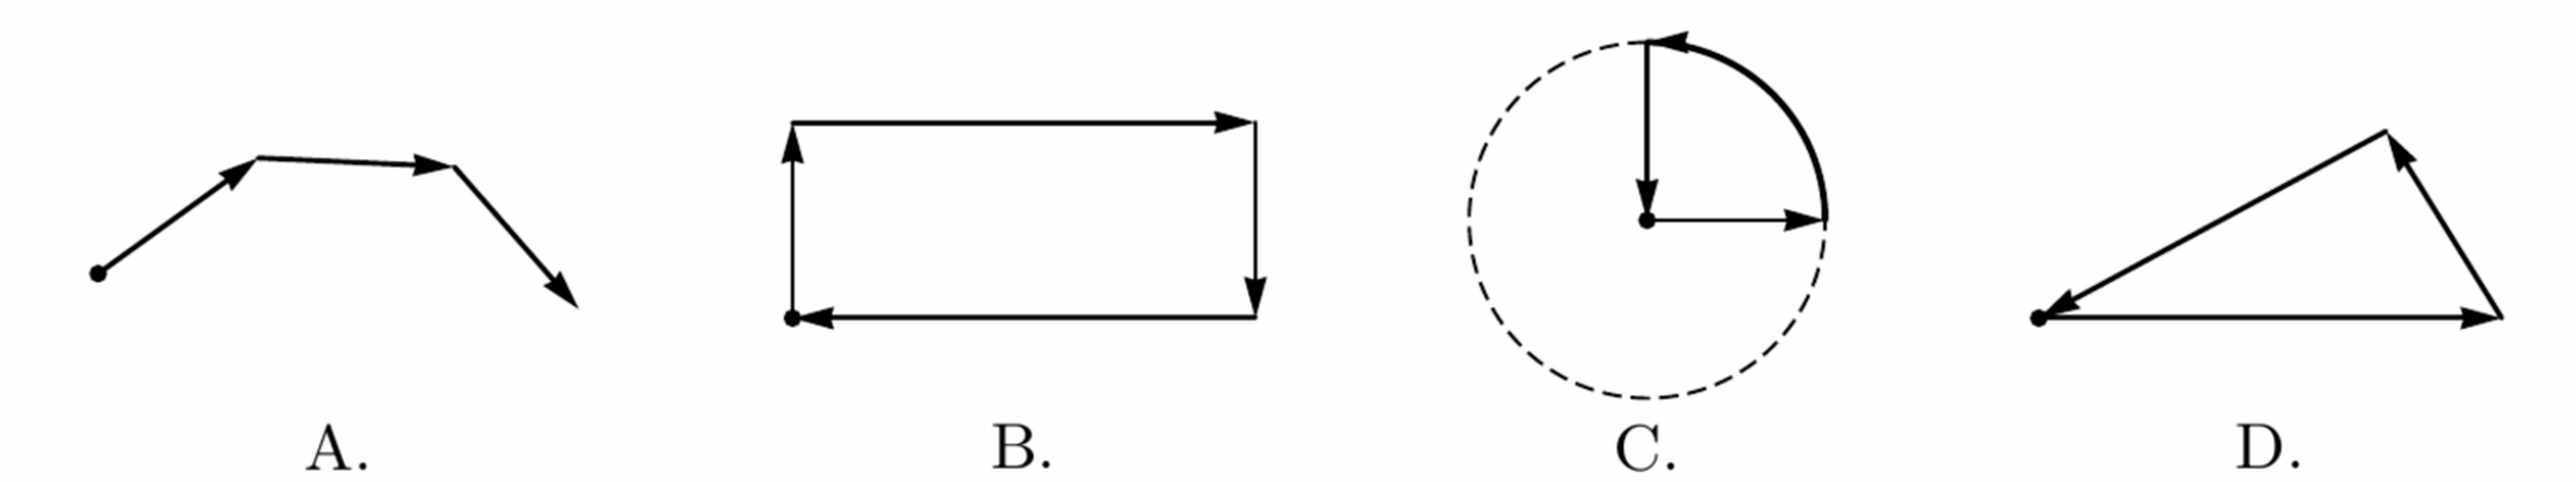
\includegraphics[width=0.86\textwidth]{figures/gao156_q14_opts.png}
\end{center}

\ifanswer
\solbegin
\step{由王老师锻炼时所走的离家距离（$S$）与行走时间（$t$）之间的函数关系图，}
\step{得在中间一段时间里，他到家的距离为定值，}
\step{故他所走的路程是一段以家为圆心的圆弧，故选 $C$.}
\solend
\fi

% === Q15 === 解析内曲线交点图（仅答案版出）；解析 4 行，故选 B
\item 已知 $a+2^a=b+\log_2 b=c+\log_3 c=k$，若 $k<1$，则\mbox{（\quad）}

\keepwithprev
A. $c<a<b$\qquad B. $a<c<b$\qquad C. $b<a<c$\qquad D. $a<b<c$

\ifanswer
\solbegin
\step{因为 $a+2^a=b+\log_2 b=c+\log_3 c=k$，}
\step{所以 $2^a=-a+k$，$\log_2 b=-b+k$，$\log_3 c=-c+k$，其中 $k<1$；}
\step{分别作出 $y=2^x$，$y=\log_2 x$，$y=\log_3 x$ 和 $y=-x+k$ 的图象，}

\begin{center}
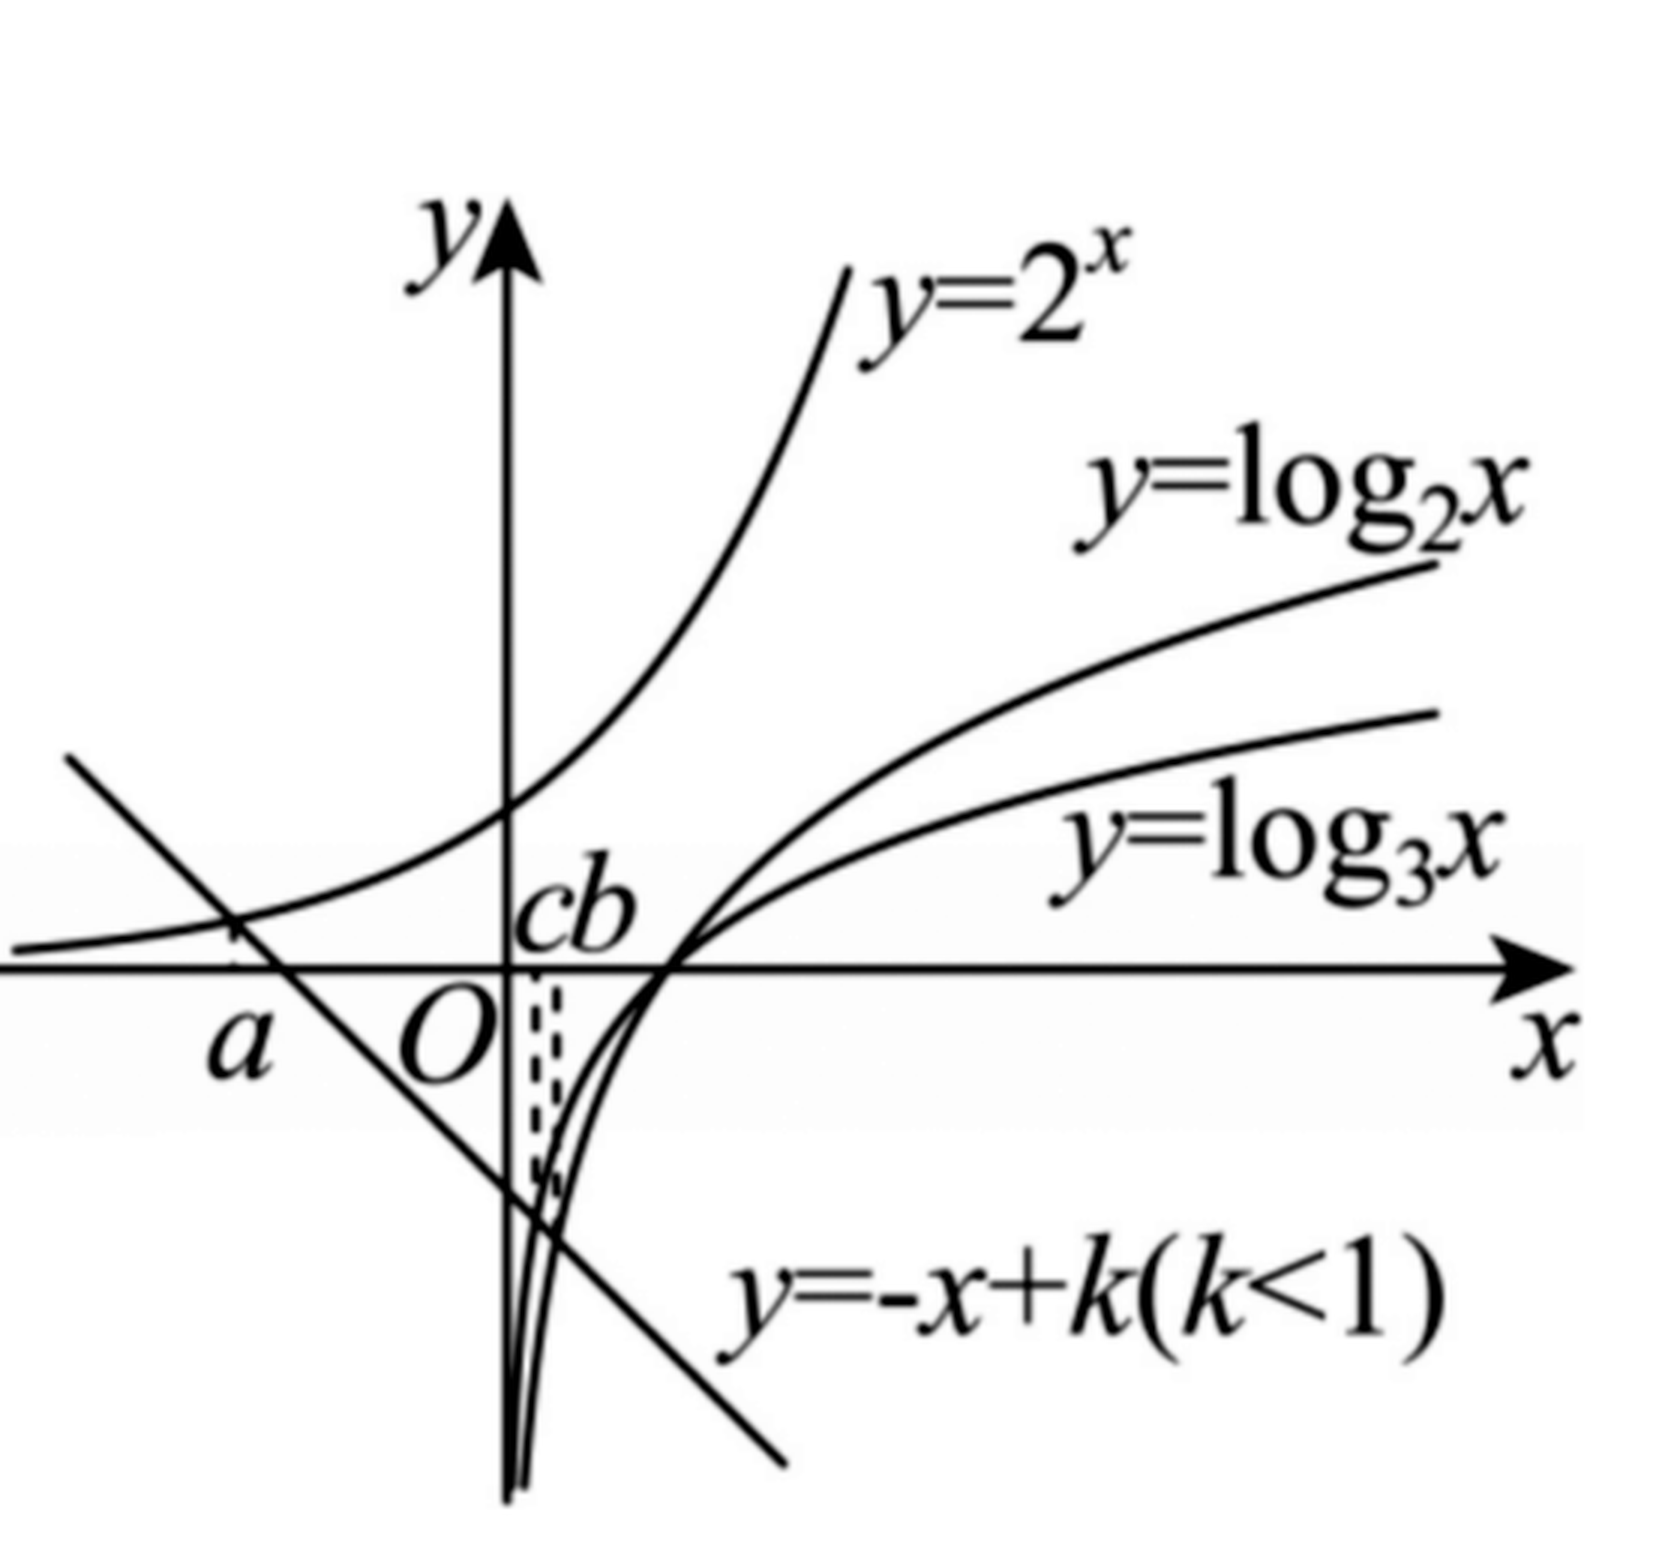
\includegraphics[width=0.52\textwidth]{figures/gao156_q15_curves.png}
\end{center}

\step{如图所示，由图象得 $a<c<b$. 故选 $B$.}
\solend
\fi

% === Q16 === ①② 文本圈数字、"一阶/二阶不动点""稳定点"自定义名词；解析 5 行，故选 A
\item 对定义域为 $I$ 的函数 $y=f(x)$，若存在 $x_0\in I$ 使得 $f(x_0)=x_0$，则称 $x_0$ 是函数 $f(x)$ 的
一阶不动点，简称不动点；若存在 $x_0\in I$ 使得 $f(f(x_0))=x_0$，则称 $x_0$ 是函数 $f(x)$ 的二阶
不动点，简称稳定点. 现有如下两个命题：①存在函数非 $y=x$ 且有无穷多个不动点；②
存在函数有无穷多个稳定点，且这些稳定点不都是不动点. 则\mbox{（\quad）}

\keepwithprev
A. ①成立，②成立\qquad\qquad B. ①成立，②不成立

C. ①不成立，②成立\qquad\qquad D. ①不成立，②不成立

\ifanswer
\solbegin
\step{①取定义在全体实数上的 $f(x)=\lvert x\rvert$，其不动点为一切非负实数，有无穷多个，}
\step{且 $f(-1)=1\ne-1$，①成立.}
\step{②取定义在全体实数上的 $g(x)=-x$，则 $g(g(x))=-(-x)=x$，}
\step{全体实数都是稳定点，而不动点只有 0，②成立.}
\step{故选 $A$.}
\solend
\fi

\end{enumerate}

\bigsec{三、解答题}

\begin{enumerate}
\setcounter{enumi}{16}

% === Q17 === $A\cap B$、$B\cap C$、\varnothing、\mid；解析 6 行
\item 设集合 $A=\{x\mid-1\leqslant x\leqslant2\}$，$B=\{x\mid2m<x<1\}$，$C=\{x\mid x<-1$ 或 $x>2\}$.

(1) 若 $A\cap B=B$，求实数 $m$ 的取值范围；

(2) 若 $B\cap C$ 中只有一个整数，求实数 $m$ 的取值范围.

\ifanswer
\solbegin
\step{(1) 当 $m\geqslant\dfrac12$ 时，$B=\varnothing$，满足 $A\cap B=B$.}
\step{当 $m<\dfrac12$ 时，$A\cap B=B$ 等价于 $2m\geqslant-1$，得 $-\dfrac12\leqslant m<\dfrac12$.}
\step{因此 $m$ 的取值范围为 $\left[-\dfrac12,+\infty\right)$.}
\step{(2) $B\cap C=\{x\mid2m<x<-1\}$，其中只有一个整数时，该整数必为 $-2$.}
\step{包含 $-2$ 且不包含 $-3$，等价于 $-3\leqslant2m<-2$，}
\step{因此 $m$ 的取值范围为 $\left[-\dfrac32,-1\right)$.}
\solend
\fi

% === Q18 === 幂函数 $x^{-\frac13}$、$m\in\R$；解析 12 行，跨 05—06 页
\item 已知幂函数 $f(x)=(3m^2-2m)x^m$（$m\in\R$）在定义域上不单调.

(1) 求函数 $f(x)$ 的解析式；

(2) 若 $f(a+1)<f(-2a+3)$，求实数 $a$ 的取值范围.

\ifanswer
\solbegin
\step{(1) 由幂函数的定义，$3m^2-2m=1$，即 $(3m+1)(m-1)=0$，得 $m=1$ 或 $m=-\dfrac13$.}
\step{当 $m=1$ 时，$f(x)=x$ 在定义域上单调递增，不合题意.}
\step{当 $m=-\dfrac13$ 时，$f(-1)=-1<f(1)=1$，而 $f(1)=1>f(8)=\dfrac12$，}
\step{故 $f(x)$ 在定义域上不单调.}
\step{因此 $f(x)=x^{-\frac13}$，定义域为 $(-\infty,0)\cup(0,+\infty)$.}
\step{(2) 有意义的条件为 $a\ne-1$ 且 $a\ne\dfrac32$.}
\step{当 $a<-1$ 时，$a+1<0<-2a+3$，有 $f(a+1)<0<f(-2a+3)$，}
\step{不等式成立.}
\step{当 $-1<a<\dfrac32$ 时，利用 $f(x)$ 在 $(0,+\infty)$ 上单调递减，}
\step{原不等式等价于 $a+1>-2a+3$，得 $\dfrac23<a<\dfrac32$.}
\step{当 $a>\dfrac32$ 时，$f(a+1)>0>f(-2a+3)$，不等式不成立.}
\step{所以 $a\in(-\infty,-1)\cup\left(\dfrac23,\dfrac32\right)$.}
\solend
\fi

% === Q19 === 两套解法（法一红字 \stepm，法二无标签）；\Delta 与 \subseteq；解析 21 行，跨 06—08 页
\item 已知 $a,c\in\R$，函数 $f(x)=\dfrac{x^2+(3a+1)x+c}{x+a}$.

(1) 若 $a=0$，求函数的定义域，并判断是否存在 $c$ 使得 $y=f(x)$ 图像关于原点对称，说明理由；

(2) 若函数过点 $(1,3)$，且函数 $y=f(x)$ 与 $x$ 轴负半轴有两个不同交点，求此时 $c$ 的值和 $a$ 的取值范围.

\ifanswer
\solbegin
\step{(1) 当 $a=0$ 时，$f(x)=\dfrac{x^2+(3a+1)x+c}{x+a}=\dfrac{x^2+x+c}{x}=x+\dfrac cx+1$，}
\step{故定义域为 $(-\infty,0)\cup(0,+\infty)$；}
\step{若存在实数 $c$，使得函数 $f(x)$ 为奇函数，则必有 $f(x)+f(-x)=0$，}
\step{而 $x+\dfrac cx+1+(-x)+\dfrac c{-x}+1=2\ne0$，}
\step{所以不存在实数 $c$，使得函数 $f(x)$ 为奇函数；}
\step{(2) 函数 $f(x)$ 的图像过点 $(1,3)$，则 $f(1)=\dfrac{1+(3a+1)+c}{1+a}=\dfrac{3a+c+2}{a+1}=3$，}
\step{解得 $c=1$，所以 $f(x)=\dfrac{x^2+(3a+1)x+1}{x+a}$，}
\stepm{法一：}{令 $f(x)=0$，则 $x^2+(3a+1)x+1=0$，此时方程有两不等负根，}
\step{则有 $\begin{cases}\Delta=(3a+1)^2-4>0\\-(3a+1)<0\end{cases}\Rightarrow\begin{cases}a>\dfrac13\text{ 或 }a<-1\\a>-\dfrac13\end{cases}\Rightarrow a>\dfrac13$，}
\step{注意到分母 $x+a\ne0$，则 $x\ne-a$，}
\step{若 $x=-a$ 也是方程 $x^2+(3a+1)x+1=0$ 的解，}
\step{代入方程 $(-a)^2+(3a+1)(-a)+1=0\Rightarrow2a^2+a-1=(a+1)(2a-1)=0$，}
\step{解得 $a=-1$ 或 $a=\dfrac12$，从而 $a\ne\dfrac12$，}
\step{综上，实数 $a$ 的取值范围为 $\left(\dfrac13,\dfrac12\right)\cup\left(\dfrac12,+\infty\right)$.}
\step{令 $g(x)=x^2+(3a+1)x+1$，与 $x$ 轴负半轴有两个交点，}
\step{则 $\begin{cases}-(3a+1)<0\\\Delta=(3a+1)^2-4>0\end{cases}\Rightarrow a>\dfrac13$.}
\step{注意到分母 $x+a\ne0$，则 $x\ne-a$，}
\step{若 $x=-a$ 也是方程 $x^2+(3a+1)x+1=0$ 的解，}
\step{代入方程 $(-a)^2+(3a+1)(-a)+1=0\Rightarrow2a^2+a-1=(a+1)(2a-1)=0$，}
\step{解得 $a=-1$ 或 $a=\dfrac12$，从而 $a\ne\dfrac12$，}
\step{综上，实数 $a$ 的取值范围为 $\left(\dfrac13,\dfrac12\right)\cup\left(\dfrac12,+\infty\right)$.}
\solend
\fi

% === Q20 === $Q$ 常数段 80000 照录；cases 与基本不等式；解析 10 行，跨 08—09 页
\item 某工厂生产某种零件的固定成本为 20000 元，每生产一个零件要增加投入 100 元，已知
总收入 $Q$（单位：元）关于产量 $x$（单位：个）满足函数：$Q=\begin{cases}400x-\dfrac12x^2,&0\leqslant x\leqslant400\\80000,&x>400\end{cases}$.

(1) 将利润 $P$（单位：元）表示为产量 $x$ 的函数；（总收入$=$总成本$+$利润）

(2) 当产量为何值时，零件的单位利润最大？最大单位利润是多少元？（单位利润$=$利润$\div$产量）

\ifanswer
\solbegin
\step{(1) 当 $0\leqslant x\leqslant400$ 时，}
\step{$P(x)=400x-\dfrac12x^2-20000-100x=-\dfrac12x^2+300x-20000$，}
\step{当 $x>400$ 时，$P(x)=80000-100x-20000=60000-100x$，}
\step{故 $P(x)=\begin{cases}-\dfrac12x^2+300x-20000,&0\leqslant x\leqslant400\\60000-100x,&x>400\end{cases}$.}
\step{(2) 设零件的单位利润为 $g(x)$，则 $g(x)=\begin{cases}-\dfrac12x-\dfrac{20000}{x}+300,&0\leqslant x\leqslant400\\\dfrac{60000}{x}-100,&x>400\end{cases}$，}
\step{当 $0\leqslant x\leqslant400$ 时，}
\step{$g(x)=300-\left(\dfrac12x+\dfrac{20000}{x}\right)\leqslant300-2\sqrt{\dfrac x2\cdot\dfrac{20000}{x}}=100$，}
\step{当且仅当 $\dfrac x2=\dfrac{20000}{x}$，即 $x=200$ 时取等号，}
\step{当 $x>400$ 时，$g(x)=\dfrac{60000}{x}-100$，此时无最值，}
\step{故当产量为 200 个，零件的单位利润最大，最大单位利润是 100 元.}
\solend
\fi

% === Q21 === 上升集定义、$D(x_0)=\{d\in\R\mid\cdots\}$、①②③ 文本圈数字、
%            \subseteq 带下划线、$-2^{-x}$；解析 19 行，跨 09—10 页
\item 已知函数 $y=f(x)$ 的定义域为 $\R$. 对任意 $x_0\in\R$，定义集合
$D(x_0)=\{d\in\R\mid f(x_0+d)>f(x_0)\}$，则称 $D(x_0)$ 为函数 $y=f(x)$ 在 $x_0$ 处的上升集.

(1) 若 $f(x)=1-x$，求 $D(-1)$；

(2) 若 $f(x)=\begin{cases}2^x,&x<0\\0,&x=0\\-2^{-x},&x>0\end{cases}$，求 $D(x)$；

(3) 设 $y=f(x)$ 满足：①当 $x<0$ 时，$f(x)=2^x$；②若 $f(x_1)\leqslant f(x_2)$，则
$D(x_2)\subseteq D(x_1)$；③当 $0<x<1$ 时，$f(x)<f(0)$. 证明：$f(0)\geqslant1$.

\ifanswer
\solbegin
\step{(1) $f(-1+d)>f(-1)\Leftrightarrow2-d>2\Leftrightarrow d<0$，所以 $D(-1)=(-\infty,0)$.}
\step{(2) 函数在 $(-\infty,0)$、$(0,+\infty)$ 上分别严格递增，}
\step{且这两个区间上的函数值分别为正、负，$f(0)=0$.}
\step{当 $x<0$ 时，$f(x+d)>f(x)\Leftrightarrow x<x+d<0\Leftrightarrow0<d<-x$，}
\step{当 $x=0$ 时，$f(d)>f(0)\Leftrightarrow d<0$，}
\step{当 $x>0$ 时，$f(x+d)>f(x)\Leftrightarrow x+d\leqslant0$ 或 $x+d>x$}
\step{$\Leftrightarrow d\leqslant-x$ 或 $d>0$，}
\step{因此 $D(x)=\begin{cases}(0,-x),&x<0\\(-\infty,0),&x=0\\(-\infty,-x]\cup(0,+\infty),&x>0\end{cases}$.}
\step{(3) 任取 $a\in(-1,0)$，}
\step{令 $d=-\dfrac a2$，则 $0<d<1$，且 $f(a+d)=2^{\frac a2}>2^a=f(a)$，}
\step{所以 $d\in D(a)$；}
\step{由③，$f(d)<f(0)$，所以 $d\notin D(0)$.}
\step{若 $f(0)\leqslant f(a)$，由②得 $D(a)\subseteq D(0)$，与上述结论矛盾.}
\step{因此，对任意 $a\in(-1,0)$，都有 $f(0)>2^a$.}
\step{特别地 $f(0)>2^{-\frac12}>0$.}
\step{若 $f(0)<1$，取 $a=\dfrac12\log_2 f(0)$，则 $-\dfrac14<a<0$，且}
\step{$2^a=\sqrt{f(0)}>f(0)$，}
\step{与 $f(0)>2^a$ 矛盾.}
\step{所以 $f(0)\geqslant1$.}
\solend
\fi

\end{enumerate}

\end{document}
"
%
% ① 原始材料：微信公众号"魔都数学加油站"文章，连载"27学年高一156"，原文标题
% "27学年高一156——2026-2027年上海市大同中学高一上期中"；
% 原文链接：https://mp.weixin.qq.com/s/xLtS5tyjCPJIWCIBohwGvw 。
% 正文为 10 张 PNG 页（01/02/03/04/05/06/07/08/09/10 各页分辨率混排
% 2560×3620 与 4762×6735，逐页按各自分辨率裁图核对）。
% 体例：讲评版——填空 3—12（10 题）、选择 13—16（4 题）、解答 17—21（5 题），
% 共 19 题，自第 3 题起编（1、2 未印在本篇）；Q3 只印【答案】、其余 18 题
% 逐题印【解析】（逐题核实，见 ②）。题目、答案、解析均据原图转录；卷面粉红色
% 水印"魔都数学加油站"及公众号页脚未录入。
%
% 卷首标题：原卷印作"2026-2027 年大同中学高一上期中"，年份区间按全稿惯例排 en dash；
% 原卷卷面未印副标题，本稿按同期中卷知识模块口径补出"集合与常用逻辑用语、不等式、函数"。
%
% ② 与原卷的排版差异：
%   ① 原文从第 3 题起，本稿保留原题号；共 19 题三节，解答题 5 题到 21；
%   ② 混合体例：第 3 题只印【答案】、无【解析】，按 高一140 第 5 题／高一145
%      第 3 题／高一151 第 7 题成例另提 \ans{}、不补造解析；其余 18 题印
%      【解析】、用 \solbegin…\solend；四道选择题答案在解析末句"故选 C／C／B／A"
%      （逐个放大复核）、括号 \mbox{（\quad）} 留空、不另提 \ans{}；答案版
%      【答案】/【解析】标记数 = 19 = 全卷题数（1 个 \ans ＋ 18 个 \solbegin）；
%   ③ 原卷卷面未印副标题，本稿按知识模块口径补出；
%   ④ 原卷填空横线按全稿惯例排 \blankline[4.4em]；选择题括号排 \mbox{（\quad）}、
%      选项段前按惯例各加 \keepwithprev；解答题不留作答区、不加 \anspace
%      （原卷为讲评版，109—113 起全稿不用 \anspace）；
%   ⑤ 数集：Q3"$x\in\R$"、Q18"$m\in\R$"、Q19"$a,c\in\R$"、Q21"定义域为 \R"
%      "任意 $x_0\in\R$""$d\in\R$"原卷印正体粗体 R，按全稿惯例归一 \R；
%      绝对值排 \lvert…\rvert（Q11 $\lvert2^x-1\rvert$、Q16 $\lvert x\rvert$），
%      集合描述竖线排 \mid（Q17 $A=\{x\mid\cdots\}$、Q21 $D(x_0)=\{d\in\R\mid\cdots\}$），
%      空集 \varnothing（Q17"$B=\varnothing$"），不等号按全稿惯例排 \leqslant／\geqslant；
%   ⑥ 子集符号逐处照录不统一：Q21 (3) 题干"$D(x_2)\subseteq D(x_1)$"与解析
%      "$D(a)\subseteq D(0)$"均印带下划线 ⊆，照录 \subseteq；本卷无单线 ⊂ 用例；
%   ⑦ 判别式：Q19 两套解法"$\Delta=(3a+1)^2-4>0$"印等腰偏高 \Delta，照录 \Delta；
%      本卷无扁三角 \triangle 用例；
%   ⑧ 红字照录为黑体：Q19 (2) 解析第一套解法行首"法一："原卷排**红色加粗**，
%      按 高一53 成例排 \stepm{法一：}{…}（加粗着色、不改黑色基调），全库无红字
%      排字先例、本稿不引入红色定义，文件头注明；第二套解法原卷直接以
%      "令 $g(x)=x^2+(3a+1)x+1$，与 $x$ 轴负半轴有两个交点，"另起，
%      **未印"法二："标签**（逐页像素级复核：07 页仅 1437—1475 一处红字，
%      08 页无红字），照录为普通 \step、不补造标签；
%   ⑨ 文本模式圈数字逐处照录：Q12 解析 ①② 两情形、Q16 两则命题与四个选项及
%      解析的 ①②、Q21 (3) 三条件 ①②③ 与解析"由③""由②"，均为印刷圈数字
%      （非 \textcircled、非数学模式），计入圈数字实测；
%   ⑩ 自定义名词照录：Q16"一阶不动点，简称不动点""二阶不动点，简称稳定点"、
%      Q21"上升集"；Q16 题干"存在函数非 $y=x$ 且有无穷多个不动点"照录；
%   ⑪ 中文弯引号照录：Q3""存在 $x\in\R$，$x^3-1\leqslant0$" 否定形式为"、
%      Q13"使"$\dfrac{x+1}{1-x}\geqslant0$"成立的必要不充分条件是"；
%      注释里一律 ASCII 引号；数学式内 CJK 用 \text{}（Q19 cases 内"或"）；
%   ⑫ 半角逗号在数学组之间是全稿惯例、非笔误，逐处照录（$a,c$、$x,y$、$a,b$
%      之类）；行末西文句点 ASCII `.`；行中全角逗号／顿号照录；
%   ⑬ 复杂式照录别简化：Q6 $\left(\dfrac{1}{\sqrt a}\right)^{\frac27}\cdot\sqrt[7]{a^3}$
%      与解析 $a^{\frac{12}{7}-\frac17+\frac37}$、Q8 $2\sqrt4+5=9$（$\sqrt4$ 未化简）、
%      Q9 $\left(\sqrt x+\dfrac{1}{\sqrt x}\right)^3$、Q12 $\dfrac{4a-(2-a)^2}{4a}$、
%      Q18 $f(8)=\dfrac12$、Q19 $2a^2+a-1=(a+1)(2a-1)=0$、Q20 $Q$ 的常数段
%      $80000$（不是 $80000-100x$）与 $2\sqrt{\dfrac x2\cdot\dfrac{20000}{x}}$、
%      Q21 $f(a+d)=2^{\frac a2}>2^a=f(a)$ 与 $2^a=\sqrt{f(0)}>f(0)$ 等；
%      \left…\right 不得拆到不同 $…$ 组（Q5 $\left(0,\dfrac12\right)$、
%      Q12 $\left[0,4+2\sqrt3\right)$、Q17 $\left[-\dfrac12,+\infty\right)$、
%      Q19 $\left(\dfrac13,\dfrac12\right)\cup\left(\dfrac12,+\infty\right)$、
%      Q20 $\left(\dfrac12x+\dfrac{20000}{x}\right)$ 等）；cases 块整体算一个印刷行；
%   ⑭ 一条 \step = 原卷解析的一个印刷行；别并折行、别拆行。跨页续印按题合并
%      （Q6 的 01 页上下题干重复印、Q8 的 01—02 页、Q12 的 02—03 页、
%      Q15 的 04 页上下、Q16 的 04—05 页、Q17 的 05 页上下、Q18 的 05—06 页、
%      Q19 的 06—08 页、Q20 的 08—09 页、Q21 的 09—10 页）；
%      跨半页重叠行（Q12 的"②若 …"、Q18 的"原不等式等价于 …"、
%      Q20 的"【解析】(1) 当 $0\leqslant x\leqslant400$ 时，"、Q21 的
%      "【解析】(1) $f(-1+d)>f(-1)\cdots$"与"与 $f(0)>2^a$ 矛盾."）
%      只算一个印刷行；
%   ⑮ 配图：全卷 3 组（逐页通读 10 页确认）——
%      · Q14 题干 S-t 梯形图（03 页右下，离家距离 S 对行走时间 t），题目配图、
%        三版都出，裁 figures/gao156_q14_st.png；
%      · Q14 四幅路线选项（04 页上部，A/B/C/D 四幅横排、C 为以家为圆心的圆弧），
%        题目配图、三版都出，合并成一张，裁 figures/gao156_q14_opts.png；
%      · Q15 解析内曲线交点图（04 页右下，$y=2^x$、$y=\log_2x$、$y=\log_3x$
%        与 $y=-x+k$），仅答案版出，裁 figures/gao156_q15_curves.png；
%      3 图均取自原卷截图，去粉色水印、去色、3×~4× LANCZOS 放大；
%      Q14 题干"题干＋两图"整块用 \needvspace 守卫推走（守卫放 \item 之前，
%      见 高一154 Q15／高一136 Q13 成例）；Q15 解析内图放 \ifanswer 内
%      \solbegin…\solend 的两 \step 之间（高一108 第 6 题／高一154 附加题 2 成例）；
%      其余各页逐页确认无其它题目配图、无解析配图、无表格；10 页下半仅水印、无正文。
%
% ③ 行数复核：一条 \step = 原卷解析的一个印刷行，cases 块作一个印刷行计。
%   逐题数（主会话逐页核对定稿）：Q3：0（只印【答案】、提 \ans{}，不计入 \step 账）；
%   Q4：1；Q5：1；Q6：1；Q7：1；Q8：3；Q9：2；Q10：2；Q11：5；Q12：12；
%   Q13：3；Q14：3；Q15：4；Q16：5；Q17：6；Q18：12；Q19：21；Q20：10；Q21：19。
%   合计 111 行（110 条 \step ＋ 1 条 \stepm），与原卷逐题印刷行相等。
%   全卷 19 题：Q3 一处 \ans{} ＋ 其余 18 题设 \solbegin…\solend，
%   答案版【答案】/【解析】标记数 = 19 = 全卷题数。
%
% ④ 页码分布（供回原图复核）：
%   卷首标题＋"一、填空题"＋Q3 题干＋【答案】、Q4 题干＋解析 1 行、
%   Q5 题干＋解析 1 行、Q6 题干首行在 01 页上半；
%   Q6 题干（重复印）＋解析 1 行、Q7 题干＋解析 1 行、Q8 题干＋解析前 2 行
%   在 01 页下半；Q8 解析末行、Q9 题干＋解析 2 行、Q10 题干＋解析 2 行、
%   Q11 题干首行在 02 页上半；Q11 题干（重复印）＋解析 5 行、
%   Q12 题干＋解析首行在 02 页下半；Q12 解析中 9 行在 03 页上半；
%   Q12 解析末 2 行＋"二、选择题"标题＋Q13 题干＋选项＋解析 3 行＋
%   Q14 题干首行在 03 页下半；Q14 题干续行＋四幅选项图＋解析 3 行＋
%   Q15 题干＋选项＋解析前 2 行＋Q16 题干在 04 页上半；
%   Q15 解析后 2 行＋曲线图＋Q16 选项＋解析前 2 行在 04 页下半；
%   Q16 解析后 3 行＋"三、解答题"标题＋Q17 题干＋两问＋解析 (1) 3 行
%   在 05 页上半；Q17 解析 (2) 3 行＋Q18 题干＋两问＋解析 (1) 首 2 行
%   在 05 页下半；Q18 解析 (1)(2) 中 8 行在 06 页上半；Q18 解析末 2 行＋
%   Q19 题干＋两问＋解析 (1) 首行在 06 页下半；Q19 解析 (1) 后 4 行＋
%   (2) 前 2 行＋法一 2 行在 07 页上半；法一后 5 行＋法二前 3 行在 07 页下半；
%   法二后 4 行＋Q20 题干＋两问＋解析 (1) 首行在 08 页上半；
%   Q20 解析 (1) 后 3 行＋(2) 前 5 行在 08 页下半；Q20 解析 (2) 末 2 行＋
%   Q21 题干＋三问＋解析 (1) 首行在 09 页上半；Q21 解析 (1)（重复印）＋
%   (2) 8 行＋(3) 首行在 09 页下半；Q21 (3) 解析中 8 行在 10 页上半；
%   Q21 (3) 末 2 行在 10 页下半。本稿按题连排，不丢行、不并折行；
%   全卷末题为第 21 题，无附加题节。
%
\documentclass[a4paper,11pt]{article}
\usepackage{common}

\begin{document}

\examtitlest[3]{2026--2027 年大同中学高一上期中}{集合与常用逻辑用语、不等式、函数}

\bigsec{一、填空题}

\begin{enumerate}
\setcounter{enumi}{2}

% === Q3 === 只印【答案】、无【解析】；R 正体粗体 \R；中文弯引号照录
\item “存在 $x\in\R$，$x^3-1\leqslant0$” 否定形式为\blankline[4.4em].

\ifanswer
\ans{对任意 $x\in\R$，$x^3-1>0$}
\fi

% === Q4 === 解析 1 行
\item 若实数 $a>0$ 且 $a\ne1$，函数 $y=a^{x-3}+1$ 的图像恒过定点 $P$，则点 $P$ 的坐标为\blankline[4.4em].

\ifanswer
\solbegin
\step{当 $x=3$ 时，$y=a^0+1=2$，与 $a$ 无关，所以定点为 $P(3,2)$.}
\solend
\fi

% === Q5 === 解析 1 行
\item 函数 $y=\dfrac{1}{3^x+2}$ 的值域是\blankline[4.4em].

\ifanswer
\solbegin
\step{$3^x\in(0,+\infty)$，因此 $3^x+2\in(2,+\infty)$，值域为 $\left(0,\dfrac12\right)$.}
\solend
\fi

% === Q6 === 根式嵌套照录；解析 1 行；题干跨 01 页上下重复印
\item 已知 $a>0$，化简 $a^{\frac{12}{7}}\cdot\left(\dfrac{1}{\sqrt a}\right)^{\frac27}\cdot\sqrt[7]{a^3}=$\blankline[4.4em].

\ifanswer
\solbegin
\step{原式 $=a^{\frac{12}{7}}\cdot a^{-\frac17}\cdot a^{\frac37}=a^{\frac{12}{7}-\frac17+\frac37}=a^2$.}
\solend
\fi

% === Q7 === 换底公式；解析 1 行
\item 已知 $\log_5 3=a$，用 $a$ 的代数式表示 $\log_{15}125=$\blankline[4.4em].

\ifanswer
\solbegin
\step{$\log_{15}125=\dfrac{\log_5 125}{\log_5 15}=\dfrac{3}{1+\log_5 3}=\dfrac{3}{1+a}$.}
\solend
\fi

% === Q8 === 基本不等式，$\sqrt4$ 照录未化简；解析 3 行，跨 01—02 页
\item 已知 $x>0$，$y>0$，且 $4x+y=xy$，则 $x+y$ 的最小值为\blankline[4.4em].

\ifanswer
\solbegin
\step{由 $4x+y=xy$，得 $\dfrac4y+\dfrac1x=1$，}
\step{则 $x+y=(x+y)\left(\dfrac4y+\dfrac1x\right)=\dfrac{4x}{y}+\dfrac yx+1+4\geqslant2\sqrt4+5=9$，}
\step{当且仅当 $\dfrac{4x}{y}=\dfrac yx$，即 $x=3$，$y=6$ 时取等号，故最小值为 9.}
\solend
\fi

% === Q9 === 解析 2 行
\item 已知 $x^{-1}+x=7$（$x>0$），则 $x^{\frac32}+x^{-\frac32}$ 的值为\blankline[4.4em].

\ifanswer
\solbegin
\step{$x>0$，有 $\sqrt x+\dfrac{1}{\sqrt x}=\sqrt{x+\dfrac1x+2}=3$，}
\step{所以 $x^{\frac32}+x^{-\frac32}=\left(\sqrt x+\dfrac{1}{\sqrt x}\right)^3-3\left(\sqrt x+\dfrac{1}{\sqrt x}\right)=27-9=18$.}
\solend
\fi

% === Q10 === $x_{\min}$；解析 2 行
\item 已知不等式 $x>\dfrac{2a+1}{a-1}$ 对任意的 $x\in[1,2]$ 恒成立，则实数 $a$ 的取值范围是\blankline[4.4em].

\ifanswer
\solbegin
\step{不等式 $x>\dfrac{2a+1}{a-1}$ 对任意的 $x\in[1,2]$ 恒成立，得 $\dfrac{2a+1}{a-1}<x_{\min}=1$，}
\step{即有 $\dfrac{a+2}{a-1}<0$，解得 $-2<a<1$，则实数 $a$ 的取值范围是 $(-2,1)$.}
\solend
\fi

% === Q11 === 分段函数 cases 与绝对值 \lvert…\rvert；解析 5 行
\item 已知函数 $f(x)=\begin{cases}\lvert2^x-1\rvert-a,&x\leqslant2\\\dfrac{3}{x-1}-a,&x>2\end{cases}$，若函数 $y=f(x)$ 图像与 $x$ 轴有三个不同交点，则实数 $a$ 的取值范围是\blankline[4.4em].

\ifanswer
\solbegin
\step{令 $g(x)=f(x)+a$.}
\step{在 $(-\infty,0)$、$[0,2]$、$(2,+\infty)$ 上，$g(x)$ 均严格单调，}
\step{值域依次为 $(0,1)$、$[0,3]$、$(0,3)$.}
\step{每段至多有一个交点，因而恰有三个不同交点，}
\step{当且仅当 $a\in(0,1)\cap[0,3]\cap(0,3)=(0,1)$.}
\solend
\fi

% === Q12 === ①② 文本圈数字、对称轴与最小值式照录；解析 12 行，跨 02—03 页
\item 已知函数 $f(x)=ax^2-(2-a)x+1$，$g(x)=x$，若对于任意实数 $x$，$f(x)$ 与 $g(x)$ 至少有一个为正数，则实数 $a$ 的取值范围是\blankline[4.4em].

\ifanswer
\solbegin
\step{当 $x>0$ 时，$g(x)>0$；当 $x<0$ 时，$g(x)<0$；}
\step{当 $x=0$ 时，$f(0)=1>0$；}
\step{因为对于任意实数 $x$，$f(x)$ 与 $g(x)$ 至少有一个为正数，}
\step{当 $x<0$ 时，因为 $g(x)<0$，所以 $f(x)=ax^2-(2-a)x+1>0$ 恒成立，}
\step{当 $a<0$ 时，显然不成立，}
\step{当 $a=0$ 时，$f(x)=-2x+1>0$，对 $x<0$ 时恒成立，满足题意，}
\step{当 $a>0$ 时，函数图象开口向上，对称轴 $x=\dfrac{2-a}{2a}$，}
\step{①若 $\dfrac{2-a}{2a}\geqslant0$，即 $0<a\leqslant2$ 时，函数 $f(x)$ 在 $(-\infty,0)$ 上严格减，$f(0)=1$，}
\step{故 $f(x)>0$ 对 $x<0$ 时恒成立，满足题意；}
\step{②若 $\dfrac{2-a}{2a}<0$，即 $a>2$ 时，$f(x)_{\min}=f\left(\dfrac{2-a}{2a}\right)=\dfrac{4a-(2-a)^2}{4a}>0$，}
\step{解得 $4-2\sqrt3<a<4+2\sqrt3$，所以 $2<a<4+2\sqrt3$.}
\step{综上，$0\leqslant a<4+2\sqrt3$，故实数 $a$ 的取值范围是 $\left[0,4+2\sqrt3\right)$.}
\solend
\fi

\end{enumerate}

\bigsec{二、选择题}

\begin{enumerate}
\setcounter{enumi}{12}

% === Q13 === 必要不充分条件；cases 块；解析 3 行，故选 C
\item 使 “$\dfrac{x+1}{1-x}\geqslant0$” 成立的必要不充分条件是\mbox{（\quad）}

\keepwithprev
A. $-1\leqslant x<1$\qquad B. $x\leqslant-1$ 或 $x>1$\qquad C. $-1\leqslant x\leqslant1$\qquad D. $x\leqslant-1$ 或 $x\geqslant0$

\ifanswer
\solbegin
\step{由不等式 $\dfrac{x+1}{1-x}\geqslant0$ 得 $\begin{cases}(x+1)(1-x)\geqslant0\\1-x\ne0\end{cases}$，解得 $-1\leqslant x<1$，}
\step{由题意结合选项，$-1\leqslant x<1\Rightarrow-1\leqslant x\leqslant1$ 成立，反之不成立，}
\step{所以 $-1\leqslant x\leqslant1$ 是 $\dfrac{x+1}{1-x}\geqslant0$ 成立的必要不充分条件. 故选 $C$.}
\solend
\fi

% === Q14 === 题干 S-t 图＋四幅路线选项（题目配图，三版都出）；守卫放 \item 之前；解析 3 行，故选 C
\needvspace{9cm}
\item 如图是王老师锻炼时所走的离家距离（$S$）与行走时间（$t$）之间的函数关系图，若
用黑点表示王老师家的位置，则王老师行走的路线可能是\mbox{（\quad）}

\begin{center}
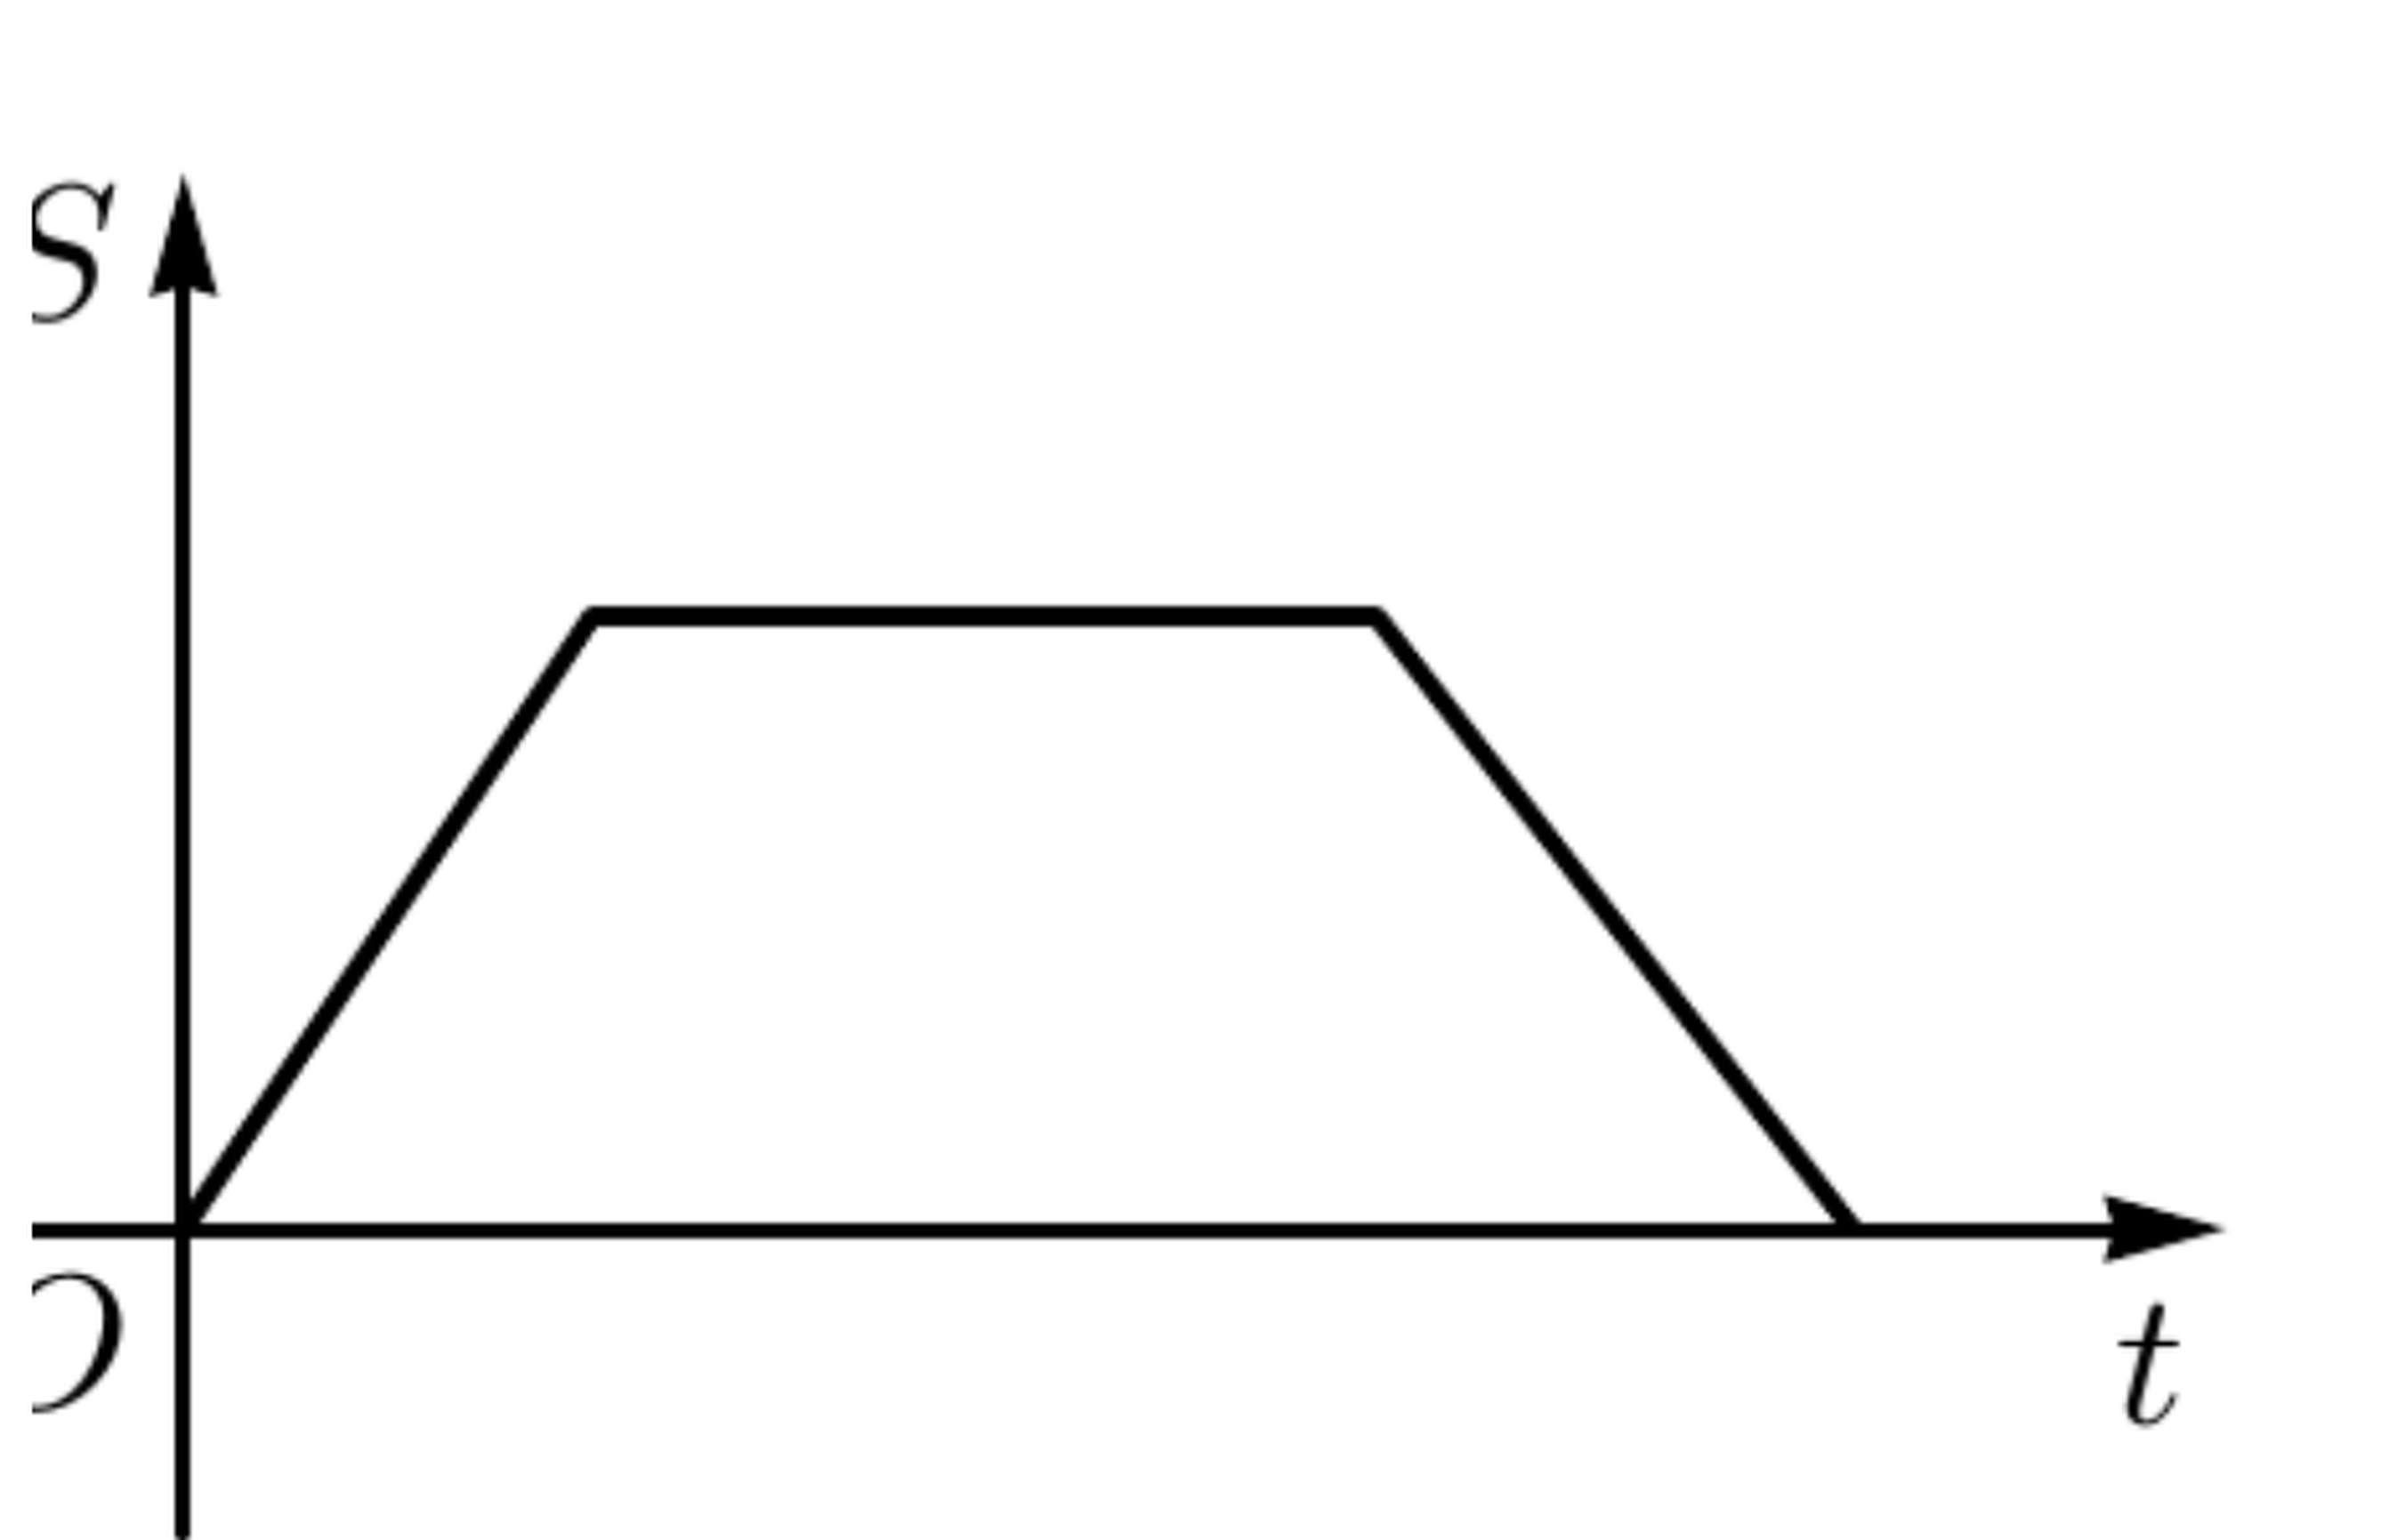
\includegraphics[width=0.34\textwidth]{figures/gao156_q14_st.png}
\end{center}

\keepwithprev
\begin{center}
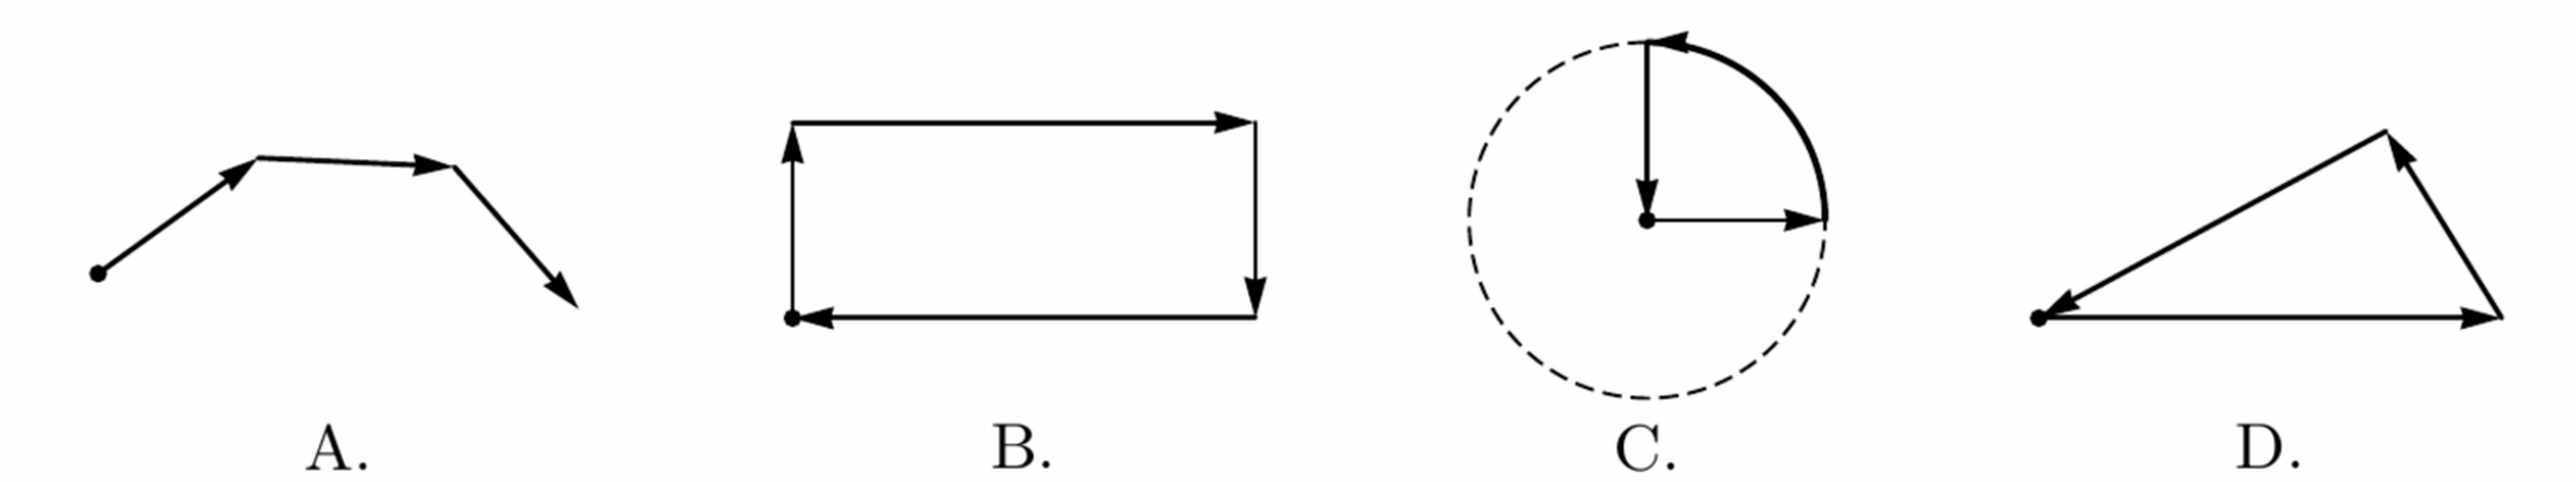
\includegraphics[width=0.86\textwidth]{figures/gao156_q14_opts.png}
\end{center}

\ifanswer
\solbegin
\step{由王老师锻炼时所走的离家距离（$S$）与行走时间（$t$）之间的函数关系图，}
\step{得在中间一段时间里，他到家的距离为定值，}
\step{故他所走的路程是一段以家为圆心的圆弧，故选 $C$.}
\solend
\fi

% === Q15 === 解析内曲线交点图（仅答案版出）；解析 4 行，故选 B
\item 已知 $a+2^a=b+\log_2 b=c+\log_3 c=k$，若 $k<1$，则\mbox{（\quad）}

\keepwithprev
A. $c<a<b$\qquad B. $a<c<b$\qquad C. $b<a<c$\qquad D. $a<b<c$

\ifanswer
\solbegin
\step{因为 $a+2^a=b+\log_2 b=c+\log_3 c=k$，}
\step{所以 $2^a=-a+k$，$\log_2 b=-b+k$，$\log_3 c=-c+k$，其中 $k<1$；}
\step{分别作出 $y=2^x$，$y=\log_2 x$，$y=\log_3 x$ 和 $y=-x+k$ 的图象，}

\begin{center}
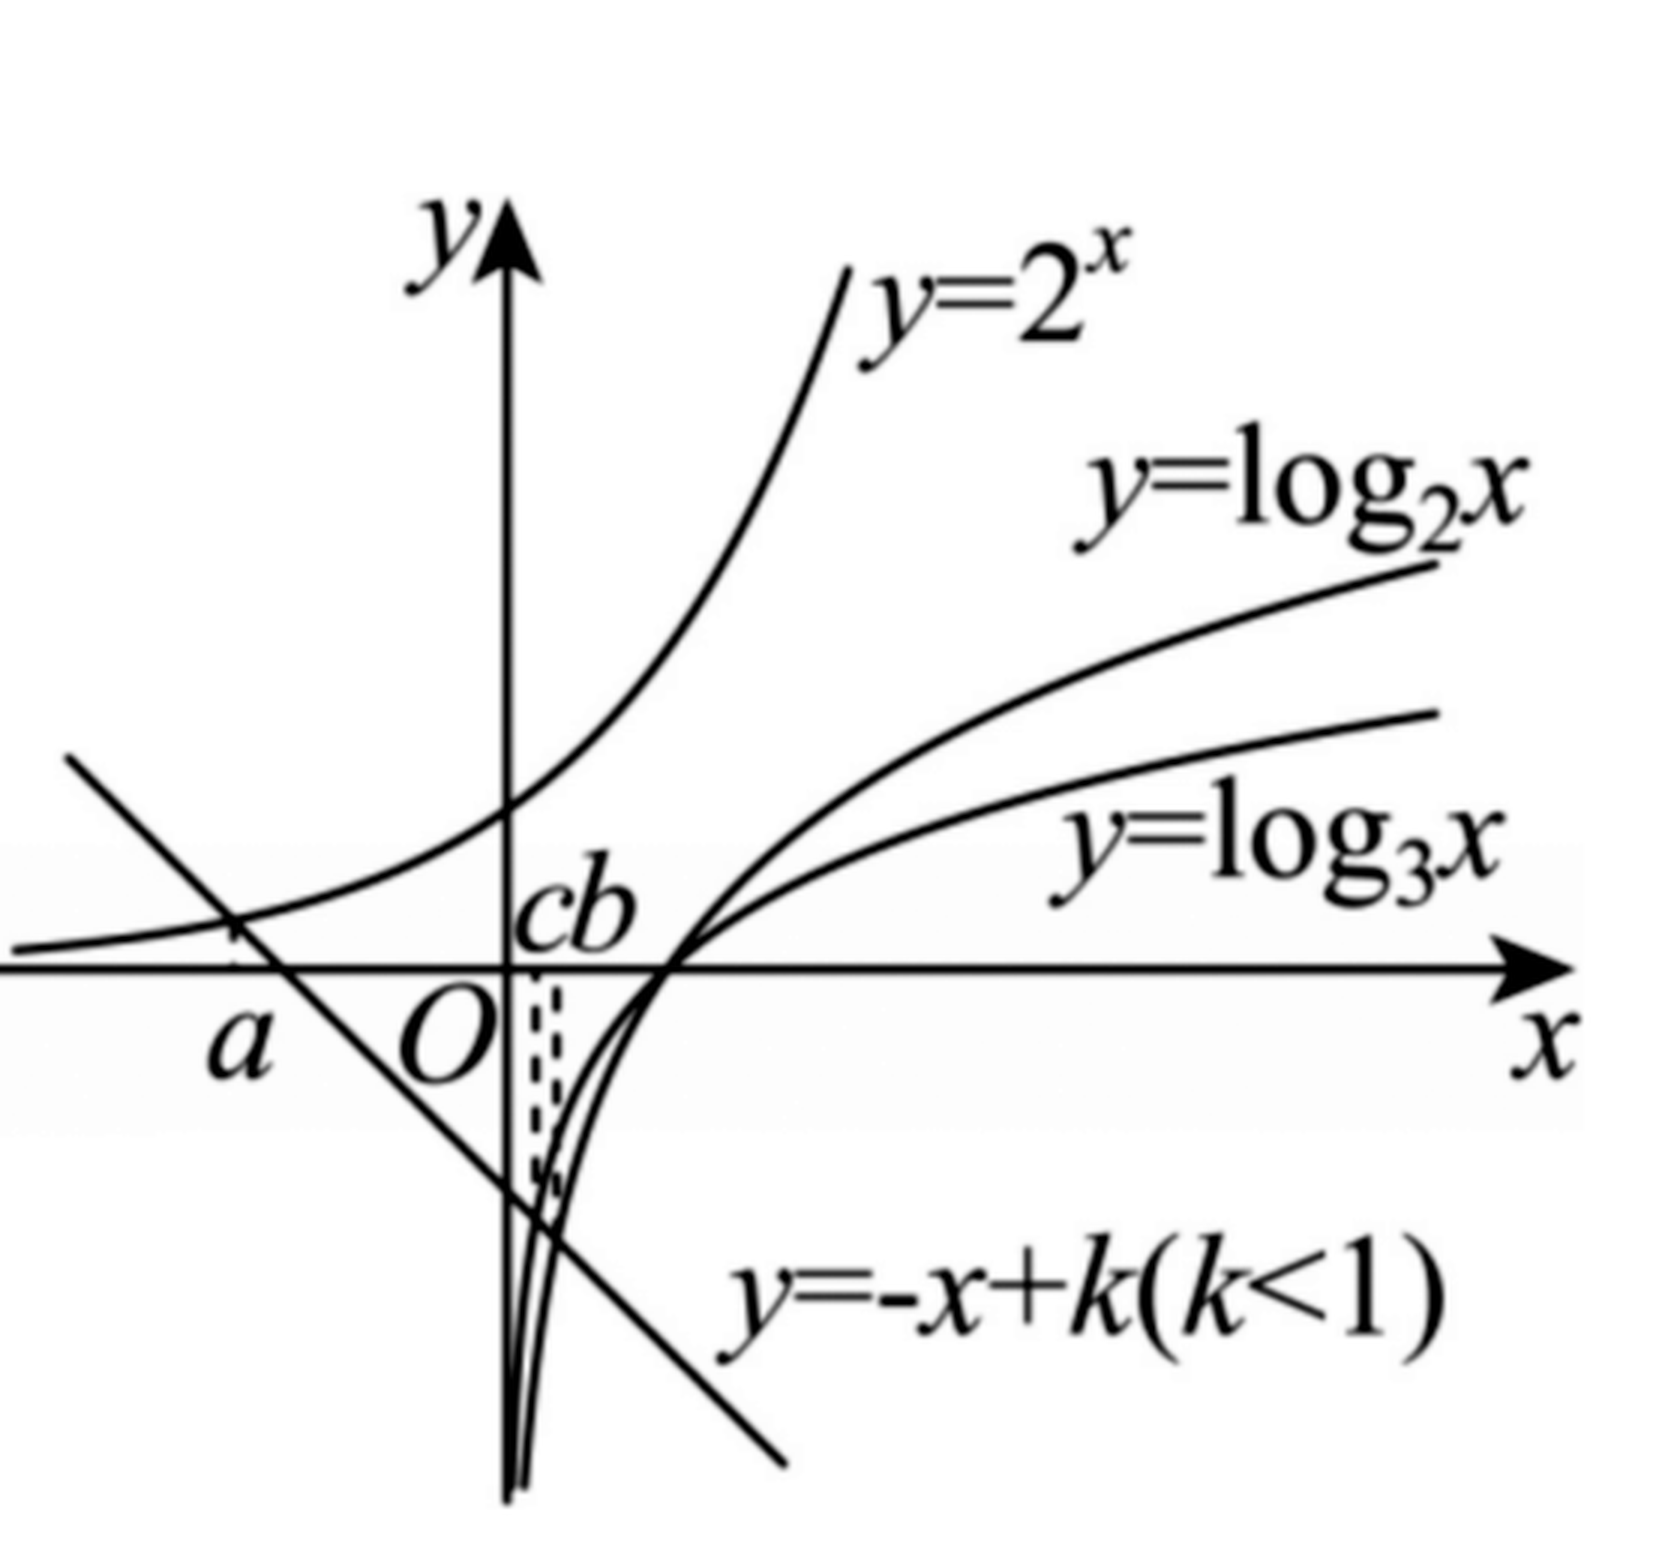
\includegraphics[width=0.52\textwidth]{figures/gao156_q15_curves.png}
\end{center}

\step{如图所示，由图象得 $a<c<b$. 故选 $B$.}
\solend
\fi

% === Q16 === ①② 文本圈数字、"一阶/二阶不动点""稳定点"自定义名词；解析 5 行，故选 A
\item 对定义域为 $I$ 的函数 $y=f(x)$，若存在 $x_0\in I$ 使得 $f(x_0)=x_0$，则称 $x_0$ 是函数 $f(x)$ 的
一阶不动点，简称不动点；若存在 $x_0\in I$ 使得 $f(f(x_0))=x_0$，则称 $x_0$ 是函数 $f(x)$ 的二阶
不动点，简称稳定点. 现有如下两个命题：①存在函数非 $y=x$ 且有无穷多个不动点；②
存在函数有无穷多个稳定点，且这些稳定点不都是不动点. 则\mbox{（\quad）}

\keepwithprev
A. ①成立，②成立\qquad\qquad B. ①成立，②不成立

C. ①不成立，②成立\qquad\qquad D. ①不成立，②不成立

\ifanswer
\solbegin
\step{①取定义在全体实数上的 $f(x)=\lvert x\rvert$，其不动点为一切非负实数，有无穷多个，}
\step{且 $f(-1)=1\ne-1$，①成立.}
\step{②取定义在全体实数上的 $g(x)=-x$，则 $g(g(x))=-(-x)=x$，}
\step{全体实数都是稳定点，而不动点只有 0，②成立.}
\step{故选 $A$.}
\solend
\fi

\end{enumerate}

\bigsec{三、解答题}

\begin{enumerate}
\setcounter{enumi}{16}

% === Q17 === $A\cap B$、$B\cap C$、\varnothing、\mid；解析 6 行
\item 设集合 $A=\{x\mid-1\leqslant x\leqslant2\}$，$B=\{x\mid2m<x<1\}$，$C=\{x\mid x<-1$ 或 $x>2\}$.

(1) 若 $A\cap B=B$，求实数 $m$ 的取值范围；

(2) 若 $B\cap C$ 中只有一个整数，求实数 $m$ 的取值范围.

\ifanswer
\solbegin
\step{(1) 当 $m\geqslant\dfrac12$ 时，$B=\varnothing$，满足 $A\cap B=B$.}
\step{当 $m<\dfrac12$ 时，$A\cap B=B$ 等价于 $2m\geqslant-1$，得 $-\dfrac12\leqslant m<\dfrac12$.}
\step{因此 $m$ 的取值范围为 $\left[-\dfrac12,+\infty\right)$.}
\step{(2) $B\cap C=\{x\mid2m<x<-1\}$，其中只有一个整数时，该整数必为 $-2$.}
\step{包含 $-2$ 且不包含 $-3$，等价于 $-3\leqslant2m<-2$，}
\step{因此 $m$ 的取值范围为 $\left[-\dfrac32,-1\right)$.}
\solend
\fi

% === Q18 === 幂函数 $x^{-\frac13}$、$m\in\R$；解析 12 行，跨 05—06 页
\item 已知幂函数 $f(x)=(3m^2-2m)x^m$（$m\in\R$）在定义域上不单调.

(1) 求函数 $f(x)$ 的解析式；

(2) 若 $f(a+1)<f(-2a+3)$，求实数 $a$ 的取值范围.

\ifanswer
\solbegin
\step{(1) 由幂函数的定义，$3m^2-2m=1$，即 $(3m+1)(m-1)=0$，得 $m=1$ 或 $m=-\dfrac13$.}
\step{当 $m=1$ 时，$f(x)=x$ 在定义域上单调递增，不合题意.}
\step{当 $m=-\dfrac13$ 时，$f(-1)=-1<f(1)=1$，而 $f(1)=1>f(8)=\dfrac12$，}
\step{故 $f(x)$ 在定义域上不单调.}
\step{因此 $f(x)=x^{-\frac13}$，定义域为 $(-\infty,0)\cup(0,+\infty)$.}
\step{(2) 有意义的条件为 $a\ne-1$ 且 $a\ne\dfrac32$.}
\step{当 $a<-1$ 时，$a+1<0<-2a+3$，有 $f(a+1)<0<f(-2a+3)$，}
\step{不等式成立.}
\step{当 $-1<a<\dfrac32$ 时，利用 $f(x)$ 在 $(0,+\infty)$ 上单调递减，}
\step{原不等式等价于 $a+1>-2a+3$，得 $\dfrac23<a<\dfrac32$.}
\step{当 $a>\dfrac32$ 时，$f(a+1)>0>f(-2a+3)$，不等式不成立.}
\step{所以 $a\in(-\infty,-1)\cup\left(\dfrac23,\dfrac32\right)$.}
\solend
\fi

% === Q19 === 两套解法（法一红字 \stepm，法二无标签）；\Delta 与 \subseteq；解析 21 行，跨 06—08 页
\item 已知 $a,c\in\R$，函数 $f(x)=\dfrac{x^2+(3a+1)x+c}{x+a}$.

(1) 若 $a=0$，求函数的定义域，并判断是否存在 $c$ 使得 $y=f(x)$ 图像关于原点对称，说明理由；

(2) 若函数过点 $(1,3)$，且函数 $y=f(x)$ 与 $x$ 轴负半轴有两个不同交点，求此时 $c$ 的值和 $a$ 的取值范围.

\ifanswer
\solbegin
\step{(1) 当 $a=0$ 时，$f(x)=\dfrac{x^2+(3a+1)x+c}{x+a}=\dfrac{x^2+x+c}{x}=x+\dfrac cx+1$，}
\step{故定义域为 $(-\infty,0)\cup(0,+\infty)$；}
\step{若存在实数 $c$，使得函数 $f(x)$ 为奇函数，则必有 $f(x)+f(-x)=0$，}
\step{而 $x+\dfrac cx+1+(-x)+\dfrac c{-x}+1=2\ne0$，}
\step{所以不存在实数 $c$，使得函数 $f(x)$ 为奇函数；}
\step{(2) 函数 $f(x)$ 的图像过点 $(1,3)$，则 $f(1)=\dfrac{1+(3a+1)+c}{1+a}=\dfrac{3a+c+2}{a+1}=3$，}
\step{解得 $c=1$，所以 $f(x)=\dfrac{x^2+(3a+1)x+1}{x+a}$，}
\stepm{法一：}{令 $f(x)=0$，则 $x^2+(3a+1)x+1=0$，此时方程有两不等负根，}
\step{则有 $\begin{cases}\Delta=(3a+1)^2-4>0\\-(3a+1)<0\end{cases}\Rightarrow\begin{cases}a>\dfrac13\text{ 或 }a<-1\\a>-\dfrac13\end{cases}\Rightarrow a>\dfrac13$，}
\step{注意到分母 $x+a\ne0$，则 $x\ne-a$，}
\step{若 $x=-a$ 也是方程 $x^2+(3a+1)x+1=0$ 的解，}
\step{代入方程 $(-a)^2+(3a+1)(-a)+1=0\Rightarrow2a^2+a-1=(a+1)(2a-1)=0$，}
\step{解得 $a=-1$ 或 $a=\dfrac12$，从而 $a\ne\dfrac12$，}
\step{综上，实数 $a$ 的取值范围为 $\left(\dfrac13,\dfrac12\right)\cup\left(\dfrac12,+\infty\right)$.}
\step{令 $g(x)=x^2+(3a+1)x+1$，与 $x$ 轴负半轴有两个交点，}
\step{则 $\begin{cases}-(3a+1)<0\\\Delta=(3a+1)^2-4>0\end{cases}\Rightarrow a>\dfrac13$.}
\step{注意到分母 $x+a\ne0$，则 $x\ne-a$，}
\step{若 $x=-a$ 也是方程 $x^2+(3a+1)x+1=0$ 的解，}
\step{代入方程 $(-a)^2+(3a+1)(-a)+1=0\Rightarrow2a^2+a-1=(a+1)(2a-1)=0$，}
\step{解得 $a=-1$ 或 $a=\dfrac12$，从而 $a\ne\dfrac12$，}
\step{综上，实数 $a$ 的取值范围为 $\left(\dfrac13,\dfrac12\right)\cup\left(\dfrac12,+\infty\right)$.}
\solend
\fi

% === Q20 === $Q$ 常数段 80000 照录；cases 与基本不等式；解析 10 行，跨 08—09 页
\item 某工厂生产某种零件的固定成本为 20000 元，每生产一个零件要增加投入 100 元，已知
总收入 $Q$（单位：元）关于产量 $x$（单位：个）满足函数：$Q=\begin{cases}400x-\dfrac12x^2,&0\leqslant x\leqslant400\\80000,&x>400\end{cases}$.

(1) 将利润 $P$（单位：元）表示为产量 $x$ 的函数；（总收入$=$总成本$+$利润）

(2) 当产量为何值时，零件的单位利润最大？最大单位利润是多少元？（单位利润$=$利润$\div$产量）

\ifanswer
\solbegin
\step{(1) 当 $0\leqslant x\leqslant400$ 时，}
\step{$P(x)=400x-\dfrac12x^2-20000-100x=-\dfrac12x^2+300x-20000$，}
\step{当 $x>400$ 时，$P(x)=80000-100x-20000=60000-100x$，}
\step{故 $P(x)=\begin{cases}-\dfrac12x^2+300x-20000,&0\leqslant x\leqslant400\\60000-100x,&x>400\end{cases}$.}
\step{(2) 设零件的单位利润为 $g(x)$，则 $g(x)=\begin{cases}-\dfrac12x-\dfrac{20000}{x}+300,&0\leqslant x\leqslant400\\\dfrac{60000}{x}-100,&x>400\end{cases}$，}
\step{当 $0\leqslant x\leqslant400$ 时，}
\step{$g(x)=300-\left(\dfrac12x+\dfrac{20000}{x}\right)\leqslant300-2\sqrt{\dfrac x2\cdot\dfrac{20000}{x}}=100$，}
\step{当且仅当 $\dfrac x2=\dfrac{20000}{x}$，即 $x=200$ 时取等号，}
\step{当 $x>400$ 时，$g(x)=\dfrac{60000}{x}-100$，此时无最值，}
\step{故当产量为 200 个，零件的单位利润最大，最大单位利润是 100 元.}
\solend
\fi

% === Q21 === 上升集定义、$D(x_0)=\{d\in\R\mid\cdots\}$、①②③ 文本圈数字、
%            \subseteq 带下划线、$-2^{-x}$；解析 19 行，跨 09—10 页
\item 已知函数 $y=f(x)$ 的定义域为 $\R$. 对任意 $x_0\in\R$，定义集合
$D(x_0)=\{d\in\R\mid f(x_0+d)>f(x_0)\}$，则称 $D(x_0)$ 为函数 $y=f(x)$ 在 $x_0$ 处的上升集.

(1) 若 $f(x)=1-x$，求 $D(-1)$；

(2) 若 $f(x)=\begin{cases}2^x,&x<0\\0,&x=0\\-2^{-x},&x>0\end{cases}$，求 $D(x)$；

(3) 设 $y=f(x)$ 满足：①当 $x<0$ 时，$f(x)=2^x$；②若 $f(x_1)\leqslant f(x_2)$，则
$D(x_2)\subseteq D(x_1)$；③当 $0<x<1$ 时，$f(x)<f(0)$. 证明：$f(0)\geqslant1$.

\ifanswer
\solbegin
\step{(1) $f(-1+d)>f(-1)\Leftrightarrow2-d>2\Leftrightarrow d<0$，所以 $D(-1)=(-\infty,0)$.}
\step{(2) 函数在 $(-\infty,0)$、$(0,+\infty)$ 上分别严格递增，}
\step{且这两个区间上的函数值分别为正、负，$f(0)=0$.}
\step{当 $x<0$ 时，$f(x+d)>f(x)\Leftrightarrow x<x+d<0\Leftrightarrow0<d<-x$，}
\step{当 $x=0$ 时，$f(d)>f(0)\Leftrightarrow d<0$，}
\step{当 $x>0$ 时，$f(x+d)>f(x)\Leftrightarrow x+d\leqslant0$ 或 $x+d>x$}
\step{$\Leftrightarrow d\leqslant-x$ 或 $d>0$，}
\step{因此 $D(x)=\begin{cases}(0,-x),&x<0\\(-\infty,0),&x=0\\(-\infty,-x]\cup(0,+\infty),&x>0\end{cases}$.}
\step{(3) 任取 $a\in(-1,0)$，}
\step{令 $d=-\dfrac a2$，则 $0<d<1$，且 $f(a+d)=2^{\frac a2}>2^a=f(a)$，}
\step{所以 $d\in D(a)$；}
\step{由③，$f(d)<f(0)$，所以 $d\notin D(0)$.}
\step{若 $f(0)\leqslant f(a)$，由②得 $D(a)\subseteq D(0)$，与上述结论矛盾.}
\step{因此，对任意 $a\in(-1,0)$，都有 $f(0)>2^a$.}
\step{特别地 $f(0)>2^{-\frac12}>0$.}
\step{若 $f(0)<1$，取 $a=\dfrac12\log_2 f(0)$，则 $-\dfrac14<a<0$，且}
\step{$2^a=\sqrt{f(0)}>f(0)$，}
\step{与 $f(0)>2^a$ 矛盾.}
\step{所以 $f(0)\geqslant1$.}
\solend
\fi

\end{enumerate}

\end{document}
"
% 紧凑版：xelatex "\def\iscompact{1}% 高一156_大同中学_期中.tex
%   —— 高一上数学"2026-2027 年大同中学高一上期中"（试卷版/答案版/紧凑版）
% 试卷版：xelatex 高一156_大同中学_期中.tex
% 答案版：xelatex "\def\isanswer{1}% 高一156_大同中学_期中.tex
%   —— 高一上数学"2026-2027 年大同中学高一上期中"（试卷版/答案版/紧凑版）
% 试卷版：xelatex 高一156_大同中学_期中.tex
% 答案版：xelatex "\def\isanswer{1}\input{高一156_大同中学_期中.tex}"
% 紧凑版：xelatex "\def\iscompact{1}\input{高一156_大同中学_期中.tex}"
%
% ① 原始材料：微信公众号"魔都数学加油站"文章，连载"27学年高一156"，原文标题
% "27学年高一156——2026-2027年上海市大同中学高一上期中"；
% 原文链接：https://mp.weixin.qq.com/s/xLtS5tyjCPJIWCIBohwGvw 。
% 正文为 10 张 PNG 页（01/02/03/04/05/06/07/08/09/10 各页分辨率混排
% 2560×3620 与 4762×6735，逐页按各自分辨率裁图核对）。
% 体例：讲评版——填空 3—12（10 题）、选择 13—16（4 题）、解答 17—21（5 题），
% 共 19 题，自第 3 题起编（1、2 未印在本篇）；Q3 只印【答案】、其余 18 题
% 逐题印【解析】（逐题核实，见 ②）。题目、答案、解析均据原图转录；卷面粉红色
% 水印"魔都数学加油站"及公众号页脚未录入。
%
% 卷首标题：原卷印作"2026-2027 年大同中学高一上期中"，年份区间按全稿惯例排 en dash；
% 原卷卷面未印副标题，本稿按同期中卷知识模块口径补出"集合与常用逻辑用语、不等式、函数"。
%
% ② 与原卷的排版差异：
%   ① 原文从第 3 题起，本稿保留原题号；共 19 题三节，解答题 5 题到 21；
%   ② 混合体例：第 3 题只印【答案】、无【解析】，按 高一140 第 5 题／高一145
%      第 3 题／高一151 第 7 题成例另提 \ans{}、不补造解析；其余 18 题印
%      【解析】、用 \solbegin…\solend；四道选择题答案在解析末句"故选 C／C／B／A"
%      （逐个放大复核）、括号 \mbox{（\quad）} 留空、不另提 \ans{}；答案版
%      【答案】/【解析】标记数 = 19 = 全卷题数（1 个 \ans ＋ 18 个 \solbegin）；
%   ③ 原卷卷面未印副标题，本稿按知识模块口径补出；
%   ④ 原卷填空横线按全稿惯例排 \blankline[4.4em]；选择题括号排 \mbox{（\quad）}、
%      选项段前按惯例各加 \keepwithprev；解答题不留作答区、不加 \anspace
%      （原卷为讲评版，109—113 起全稿不用 \anspace）；
%   ⑤ 数集：Q3"$x\in\R$"、Q18"$m\in\R$"、Q19"$a,c\in\R$"、Q21"定义域为 \R"
%      "任意 $x_0\in\R$""$d\in\R$"原卷印正体粗体 R，按全稿惯例归一 \R；
%      绝对值排 \lvert…\rvert（Q11 $\lvert2^x-1\rvert$、Q16 $\lvert x\rvert$），
%      集合描述竖线排 \mid（Q17 $A=\{x\mid\cdots\}$、Q21 $D(x_0)=\{d\in\R\mid\cdots\}$），
%      空集 \varnothing（Q17"$B=\varnothing$"），不等号按全稿惯例排 \leqslant／\geqslant；
%   ⑥ 子集符号逐处照录不统一：Q21 (3) 题干"$D(x_2)\subseteq D(x_1)$"与解析
%      "$D(a)\subseteq D(0)$"均印带下划线 ⊆，照录 \subseteq；本卷无单线 ⊂ 用例；
%   ⑦ 判别式：Q19 两套解法"$\Delta=(3a+1)^2-4>0$"印等腰偏高 \Delta，照录 \Delta；
%      本卷无扁三角 \triangle 用例；
%   ⑧ 红字照录为黑体：Q19 (2) 解析第一套解法行首"法一："原卷排**红色加粗**，
%      按 高一53 成例排 \stepm{法一：}{…}（加粗着色、不改黑色基调），全库无红字
%      排字先例、本稿不引入红色定义，文件头注明；第二套解法原卷直接以
%      "令 $g(x)=x^2+(3a+1)x+1$，与 $x$ 轴负半轴有两个交点，"另起，
%      **未印"法二："标签**（逐页像素级复核：07 页仅 1437—1475 一处红字，
%      08 页无红字），照录为普通 \step、不补造标签；
%   ⑨ 文本模式圈数字逐处照录：Q12 解析 ①② 两情形、Q16 两则命题与四个选项及
%      解析的 ①②、Q21 (3) 三条件 ①②③ 与解析"由③""由②"，均为印刷圈数字
%      （非 \textcircled、非数学模式），计入圈数字实测；
%   ⑩ 自定义名词照录：Q16"一阶不动点，简称不动点""二阶不动点，简称稳定点"、
%      Q21"上升集"；Q16 题干"存在函数非 $y=x$ 且有无穷多个不动点"照录；
%   ⑪ 中文弯引号照录：Q3""存在 $x\in\R$，$x^3-1\leqslant0$" 否定形式为"、
%      Q13"使"$\dfrac{x+1}{1-x}\geqslant0$"成立的必要不充分条件是"；
%      注释里一律 ASCII 引号；数学式内 CJK 用 \text{}（Q19 cases 内"或"）；
%   ⑫ 半角逗号在数学组之间是全稿惯例、非笔误，逐处照录（$a,c$、$x,y$、$a,b$
%      之类）；行末西文句点 ASCII `.`；行中全角逗号／顿号照录；
%   ⑬ 复杂式照录别简化：Q6 $\left(\dfrac{1}{\sqrt a}\right)^{\frac27}\cdot\sqrt[7]{a^3}$
%      与解析 $a^{\frac{12}{7}-\frac17+\frac37}$、Q8 $2\sqrt4+5=9$（$\sqrt4$ 未化简）、
%      Q9 $\left(\sqrt x+\dfrac{1}{\sqrt x}\right)^3$、Q12 $\dfrac{4a-(2-a)^2}{4a}$、
%      Q18 $f(8)=\dfrac12$、Q19 $2a^2+a-1=(a+1)(2a-1)=0$、Q20 $Q$ 的常数段
%      $80000$（不是 $80000-100x$）与 $2\sqrt{\dfrac x2\cdot\dfrac{20000}{x}}$、
%      Q21 $f(a+d)=2^{\frac a2}>2^a=f(a)$ 与 $2^a=\sqrt{f(0)}>f(0)$ 等；
%      \left…\right 不得拆到不同 $…$ 组（Q5 $\left(0,\dfrac12\right)$、
%      Q12 $\left[0,4+2\sqrt3\right)$、Q17 $\left[-\dfrac12,+\infty\right)$、
%      Q19 $\left(\dfrac13,\dfrac12\right)\cup\left(\dfrac12,+\infty\right)$、
%      Q20 $\left(\dfrac12x+\dfrac{20000}{x}\right)$ 等）；cases 块整体算一个印刷行；
%   ⑭ 一条 \step = 原卷解析的一个印刷行；别并折行、别拆行。跨页续印按题合并
%      （Q6 的 01 页上下题干重复印、Q8 的 01—02 页、Q12 的 02—03 页、
%      Q15 的 04 页上下、Q16 的 04—05 页、Q17 的 05 页上下、Q18 的 05—06 页、
%      Q19 的 06—08 页、Q20 的 08—09 页、Q21 的 09—10 页）；
%      跨半页重叠行（Q12 的"②若 …"、Q18 的"原不等式等价于 …"、
%      Q20 的"【解析】(1) 当 $0\leqslant x\leqslant400$ 时，"、Q21 的
%      "【解析】(1) $f(-1+d)>f(-1)\cdots$"与"与 $f(0)>2^a$ 矛盾."）
%      只算一个印刷行；
%   ⑮ 配图：全卷 3 组（逐页通读 10 页确认）——
%      · Q14 题干 S-t 梯形图（03 页右下，离家距离 S 对行走时间 t），题目配图、
%        三版都出，裁 figures/gao156_q14_st.png；
%      · Q14 四幅路线选项（04 页上部，A/B/C/D 四幅横排、C 为以家为圆心的圆弧），
%        题目配图、三版都出，合并成一张，裁 figures/gao156_q14_opts.png；
%      · Q15 解析内曲线交点图（04 页右下，$y=2^x$、$y=\log_2x$、$y=\log_3x$
%        与 $y=-x+k$），仅答案版出，裁 figures/gao156_q15_curves.png；
%      3 图均取自原卷截图，去粉色水印、去色、3×~4× LANCZOS 放大；
%      Q14 题干"题干＋两图"整块用 \needvspace 守卫推走（守卫放 \item 之前，
%      见 高一154 Q15／高一136 Q13 成例）；Q15 解析内图放 \ifanswer 内
%      \solbegin…\solend 的两 \step 之间（高一108 第 6 题／高一154 附加题 2 成例）；
%      其余各页逐页确认无其它题目配图、无解析配图、无表格；10 页下半仅水印、无正文。
%
% ③ 行数复核：一条 \step = 原卷解析的一个印刷行，cases 块作一个印刷行计。
%   逐题数（主会话逐页核对定稿）：Q3：0（只印【答案】、提 \ans{}，不计入 \step 账）；
%   Q4：1；Q5：1；Q6：1；Q7：1；Q8：3；Q9：2；Q10：2；Q11：5；Q12：12；
%   Q13：3；Q14：3；Q15：4；Q16：5；Q17：6；Q18：12；Q19：21；Q20：10；Q21：19。
%   合计 111 行（110 条 \step ＋ 1 条 \stepm），与原卷逐题印刷行相等。
%   全卷 19 题：Q3 一处 \ans{} ＋ 其余 18 题设 \solbegin…\solend，
%   答案版【答案】/【解析】标记数 = 19 = 全卷题数。
%
% ④ 页码分布（供回原图复核）：
%   卷首标题＋"一、填空题"＋Q3 题干＋【答案】、Q4 题干＋解析 1 行、
%   Q5 题干＋解析 1 行、Q6 题干首行在 01 页上半；
%   Q6 题干（重复印）＋解析 1 行、Q7 题干＋解析 1 行、Q8 题干＋解析前 2 行
%   在 01 页下半；Q8 解析末行、Q9 题干＋解析 2 行、Q10 题干＋解析 2 行、
%   Q11 题干首行在 02 页上半；Q11 题干（重复印）＋解析 5 行、
%   Q12 题干＋解析首行在 02 页下半；Q12 解析中 9 行在 03 页上半；
%   Q12 解析末 2 行＋"二、选择题"标题＋Q13 题干＋选项＋解析 3 行＋
%   Q14 题干首行在 03 页下半；Q14 题干续行＋四幅选项图＋解析 3 行＋
%   Q15 题干＋选项＋解析前 2 行＋Q16 题干在 04 页上半；
%   Q15 解析后 2 行＋曲线图＋Q16 选项＋解析前 2 行在 04 页下半；
%   Q16 解析后 3 行＋"三、解答题"标题＋Q17 题干＋两问＋解析 (1) 3 行
%   在 05 页上半；Q17 解析 (2) 3 行＋Q18 题干＋两问＋解析 (1) 首 2 行
%   在 05 页下半；Q18 解析 (1)(2) 中 8 行在 06 页上半；Q18 解析末 2 行＋
%   Q19 题干＋两问＋解析 (1) 首行在 06 页下半；Q19 解析 (1) 后 4 行＋
%   (2) 前 2 行＋法一 2 行在 07 页上半；法一后 5 行＋法二前 3 行在 07 页下半；
%   法二后 4 行＋Q20 题干＋两问＋解析 (1) 首行在 08 页上半；
%   Q20 解析 (1) 后 3 行＋(2) 前 5 行在 08 页下半；Q20 解析 (2) 末 2 行＋
%   Q21 题干＋三问＋解析 (1) 首行在 09 页上半；Q21 解析 (1)（重复印）＋
%   (2) 8 行＋(3) 首行在 09 页下半；Q21 (3) 解析中 8 行在 10 页上半；
%   Q21 (3) 末 2 行在 10 页下半。本稿按题连排，不丢行、不并折行；
%   全卷末题为第 21 题，无附加题节。
%
\documentclass[a4paper,11pt]{article}
\usepackage{common}

\begin{document}

\examtitlest[3]{2026--2027 年大同中学高一上期中}{集合与常用逻辑用语、不等式、函数}

\bigsec{一、填空题}

\begin{enumerate}
\setcounter{enumi}{2}

% === Q3 === 只印【答案】、无【解析】；R 正体粗体 \R；中文弯引号照录
\item “存在 $x\in\R$，$x^3-1\leqslant0$” 否定形式为\blankline[4.4em].

\ifanswer
\ans{对任意 $x\in\R$，$x^3-1>0$}
\fi

% === Q4 === 解析 1 行
\item 若实数 $a>0$ 且 $a\ne1$，函数 $y=a^{x-3}+1$ 的图像恒过定点 $P$，则点 $P$ 的坐标为\blankline[4.4em].

\ifanswer
\solbegin
\step{当 $x=3$ 时，$y=a^0+1=2$，与 $a$ 无关，所以定点为 $P(3,2)$.}
\solend
\fi

% === Q5 === 解析 1 行
\item 函数 $y=\dfrac{1}{3^x+2}$ 的值域是\blankline[4.4em].

\ifanswer
\solbegin
\step{$3^x\in(0,+\infty)$，因此 $3^x+2\in(2,+\infty)$，值域为 $\left(0,\dfrac12\right)$.}
\solend
\fi

% === Q6 === 根式嵌套照录；解析 1 行；题干跨 01 页上下重复印
\item 已知 $a>0$，化简 $a^{\frac{12}{7}}\cdot\left(\dfrac{1}{\sqrt a}\right)^{\frac27}\cdot\sqrt[7]{a^3}=$\blankline[4.4em].

\ifanswer
\solbegin
\step{原式 $=a^{\frac{12}{7}}\cdot a^{-\frac17}\cdot a^{\frac37}=a^{\frac{12}{7}-\frac17+\frac37}=a^2$.}
\solend
\fi

% === Q7 === 换底公式；解析 1 行
\item 已知 $\log_5 3=a$，用 $a$ 的代数式表示 $\log_{15}125=$\blankline[4.4em].

\ifanswer
\solbegin
\step{$\log_{15}125=\dfrac{\log_5 125}{\log_5 15}=\dfrac{3}{1+\log_5 3}=\dfrac{3}{1+a}$.}
\solend
\fi

% === Q8 === 基本不等式，$\sqrt4$ 照录未化简；解析 3 行，跨 01—02 页
\item 已知 $x>0$，$y>0$，且 $4x+y=xy$，则 $x+y$ 的最小值为\blankline[4.4em].

\ifanswer
\solbegin
\step{由 $4x+y=xy$，得 $\dfrac4y+\dfrac1x=1$，}
\step{则 $x+y=(x+y)\left(\dfrac4y+\dfrac1x\right)=\dfrac{4x}{y}+\dfrac yx+1+4\geqslant2\sqrt4+5=9$，}
\step{当且仅当 $\dfrac{4x}{y}=\dfrac yx$，即 $x=3$，$y=6$ 时取等号，故最小值为 9.}
\solend
\fi

% === Q9 === 解析 2 行
\item 已知 $x^{-1}+x=7$（$x>0$），则 $x^{\frac32}+x^{-\frac32}$ 的值为\blankline[4.4em].

\ifanswer
\solbegin
\step{$x>0$，有 $\sqrt x+\dfrac{1}{\sqrt x}=\sqrt{x+\dfrac1x+2}=3$，}
\step{所以 $x^{\frac32}+x^{-\frac32}=\left(\sqrt x+\dfrac{1}{\sqrt x}\right)^3-3\left(\sqrt x+\dfrac{1}{\sqrt x}\right)=27-9=18$.}
\solend
\fi

% === Q10 === $x_{\min}$；解析 2 行
\item 已知不等式 $x>\dfrac{2a+1}{a-1}$ 对任意的 $x\in[1,2]$ 恒成立，则实数 $a$ 的取值范围是\blankline[4.4em].

\ifanswer
\solbegin
\step{不等式 $x>\dfrac{2a+1}{a-1}$ 对任意的 $x\in[1,2]$ 恒成立，得 $\dfrac{2a+1}{a-1}<x_{\min}=1$，}
\step{即有 $\dfrac{a+2}{a-1}<0$，解得 $-2<a<1$，则实数 $a$ 的取值范围是 $(-2,1)$.}
\solend
\fi

% === Q11 === 分段函数 cases 与绝对值 \lvert…\rvert；解析 5 行
\item 已知函数 $f(x)=\begin{cases}\lvert2^x-1\rvert-a,&x\leqslant2\\\dfrac{3}{x-1}-a,&x>2\end{cases}$，若函数 $y=f(x)$ 图像与 $x$ 轴有三个不同交点，则实数 $a$ 的取值范围是\blankline[4.4em].

\ifanswer
\solbegin
\step{令 $g(x)=f(x)+a$.}
\step{在 $(-\infty,0)$、$[0,2]$、$(2,+\infty)$ 上，$g(x)$ 均严格单调，}
\step{值域依次为 $(0,1)$、$[0,3]$、$(0,3)$.}
\step{每段至多有一个交点，因而恰有三个不同交点，}
\step{当且仅当 $a\in(0,1)\cap[0,3]\cap(0,3)=(0,1)$.}
\solend
\fi

% === Q12 === ①② 文本圈数字、对称轴与最小值式照录；解析 12 行，跨 02—03 页
\item 已知函数 $f(x)=ax^2-(2-a)x+1$，$g(x)=x$，若对于任意实数 $x$，$f(x)$ 与 $g(x)$ 至少有一个为正数，则实数 $a$ 的取值范围是\blankline[4.4em].

\ifanswer
\solbegin
\step{当 $x>0$ 时，$g(x)>0$；当 $x<0$ 时，$g(x)<0$；}
\step{当 $x=0$ 时，$f(0)=1>0$；}
\step{因为对于任意实数 $x$，$f(x)$ 与 $g(x)$ 至少有一个为正数，}
\step{当 $x<0$ 时，因为 $g(x)<0$，所以 $f(x)=ax^2-(2-a)x+1>0$ 恒成立，}
\step{当 $a<0$ 时，显然不成立，}
\step{当 $a=0$ 时，$f(x)=-2x+1>0$，对 $x<0$ 时恒成立，满足题意，}
\step{当 $a>0$ 时，函数图象开口向上，对称轴 $x=\dfrac{2-a}{2a}$，}
\step{①若 $\dfrac{2-a}{2a}\geqslant0$，即 $0<a\leqslant2$ 时，函数 $f(x)$ 在 $(-\infty,0)$ 上严格减，$f(0)=1$，}
\step{故 $f(x)>0$ 对 $x<0$ 时恒成立，满足题意；}
\step{②若 $\dfrac{2-a}{2a}<0$，即 $a>2$ 时，$f(x)_{\min}=f\left(\dfrac{2-a}{2a}\right)=\dfrac{4a-(2-a)^2}{4a}>0$，}
\step{解得 $4-2\sqrt3<a<4+2\sqrt3$，所以 $2<a<4+2\sqrt3$.}
\step{综上，$0\leqslant a<4+2\sqrt3$，故实数 $a$ 的取值范围是 $\left[0,4+2\sqrt3\right)$.}
\solend
\fi

\end{enumerate}

\bigsec{二、选择题}

\begin{enumerate}
\setcounter{enumi}{12}

% === Q13 === 必要不充分条件；cases 块；解析 3 行，故选 C
\item 使 “$\dfrac{x+1}{1-x}\geqslant0$” 成立的必要不充分条件是\mbox{（\quad）}

\keepwithprev
A. $-1\leqslant x<1$\qquad B. $x\leqslant-1$ 或 $x>1$\qquad C. $-1\leqslant x\leqslant1$\qquad D. $x\leqslant-1$ 或 $x\geqslant0$

\ifanswer
\solbegin
\step{由不等式 $\dfrac{x+1}{1-x}\geqslant0$ 得 $\begin{cases}(x+1)(1-x)\geqslant0\\1-x\ne0\end{cases}$，解得 $-1\leqslant x<1$，}
\step{由题意结合选项，$-1\leqslant x<1\Rightarrow-1\leqslant x\leqslant1$ 成立，反之不成立，}
\step{所以 $-1\leqslant x\leqslant1$ 是 $\dfrac{x+1}{1-x}\geqslant0$ 成立的必要不充分条件. 故选 $C$.}
\solend
\fi

% === Q14 === 题干 S-t 图＋四幅路线选项（题目配图，三版都出）；守卫放 \item 之前；解析 3 行，故选 C
\needvspace{9cm}
\item 如图是王老师锻炼时所走的离家距离（$S$）与行走时间（$t$）之间的函数关系图，若
用黑点表示王老师家的位置，则王老师行走的路线可能是\mbox{（\quad）}

\begin{center}
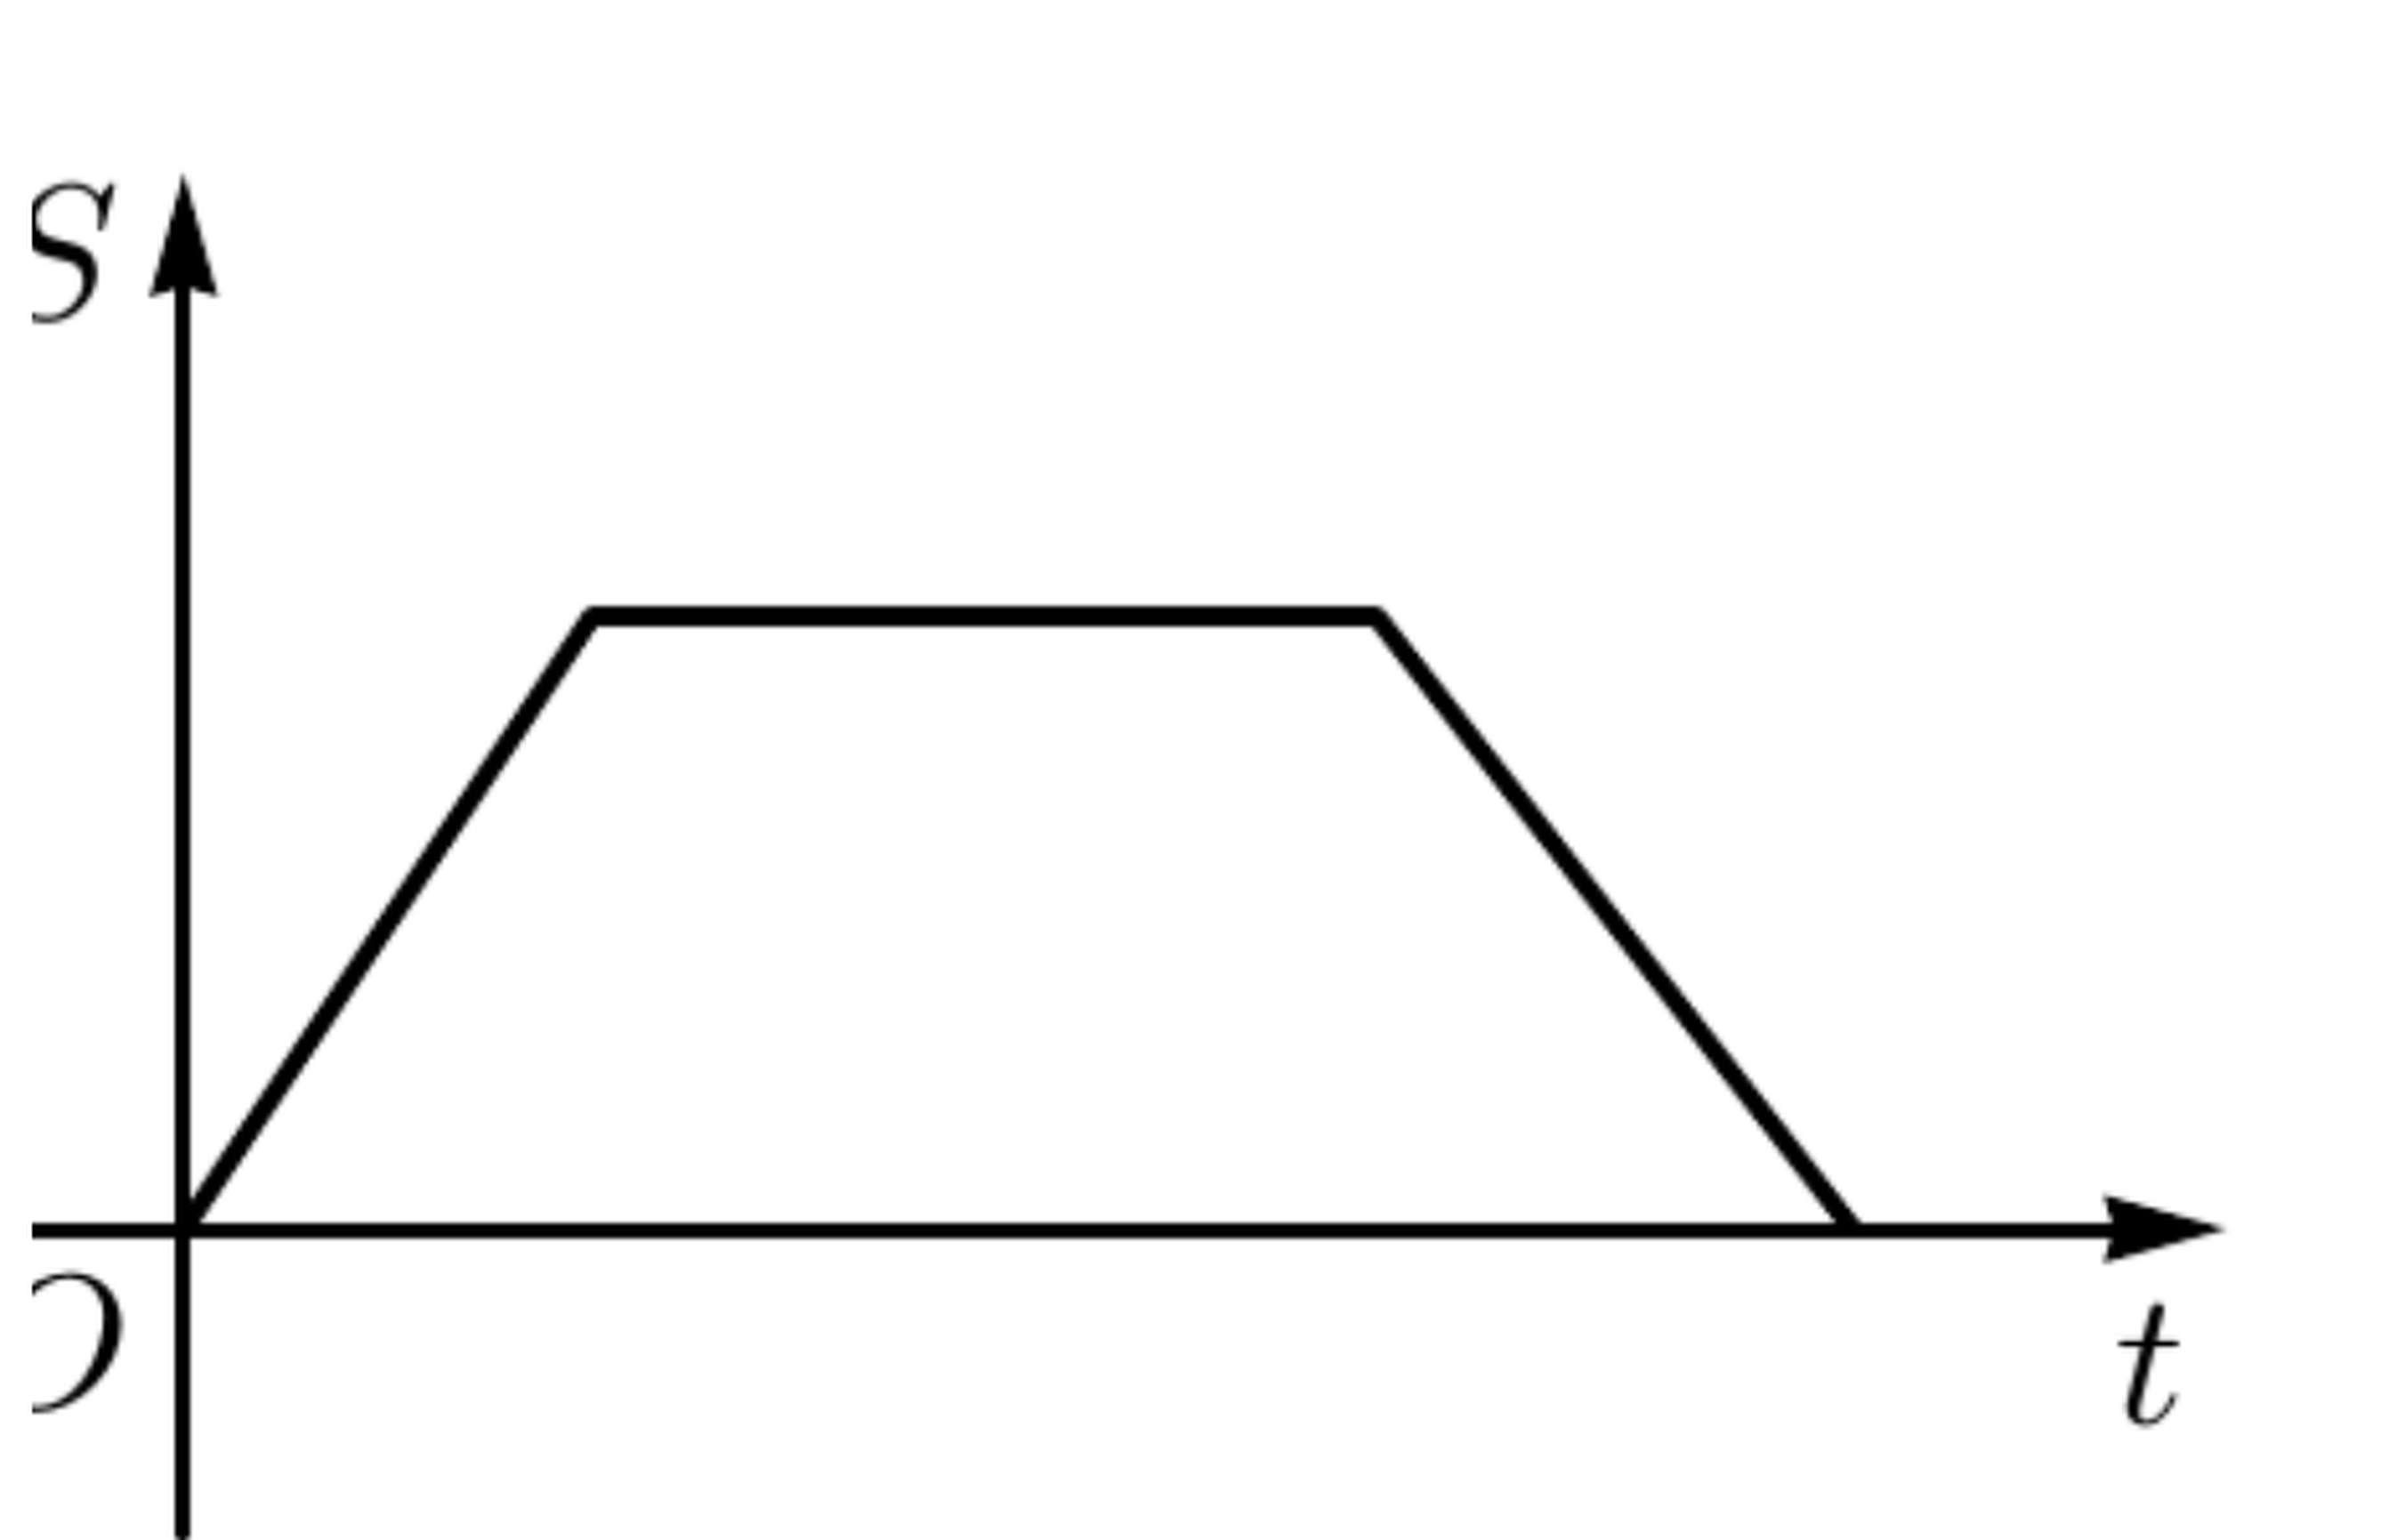
\includegraphics[width=0.34\textwidth]{figures/gao156_q14_st.png}
\end{center}

\keepwithprev
\begin{center}
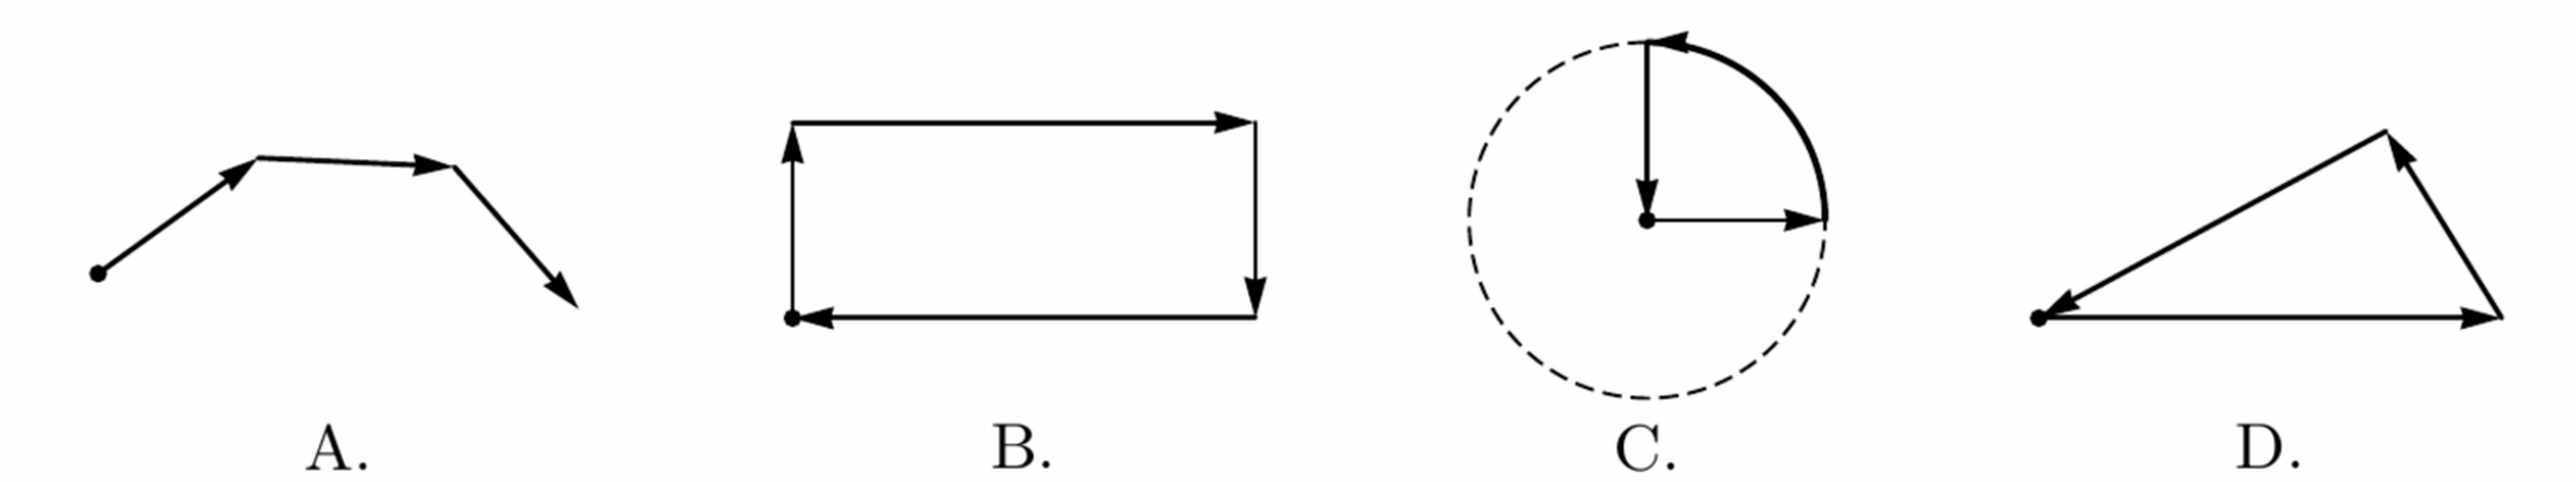
\includegraphics[width=0.86\textwidth]{figures/gao156_q14_opts.png}
\end{center}

\ifanswer
\solbegin
\step{由王老师锻炼时所走的离家距离（$S$）与行走时间（$t$）之间的函数关系图，}
\step{得在中间一段时间里，他到家的距离为定值，}
\step{故他所走的路程是一段以家为圆心的圆弧，故选 $C$.}
\solend
\fi

% === Q15 === 解析内曲线交点图（仅答案版出）；解析 4 行，故选 B
\item 已知 $a+2^a=b+\log_2 b=c+\log_3 c=k$，若 $k<1$，则\mbox{（\quad）}

\keepwithprev
A. $c<a<b$\qquad B. $a<c<b$\qquad C. $b<a<c$\qquad D. $a<b<c$

\ifanswer
\solbegin
\step{因为 $a+2^a=b+\log_2 b=c+\log_3 c=k$，}
\step{所以 $2^a=-a+k$，$\log_2 b=-b+k$，$\log_3 c=-c+k$，其中 $k<1$；}
\step{分别作出 $y=2^x$，$y=\log_2 x$，$y=\log_3 x$ 和 $y=-x+k$ 的图象，}

\begin{center}
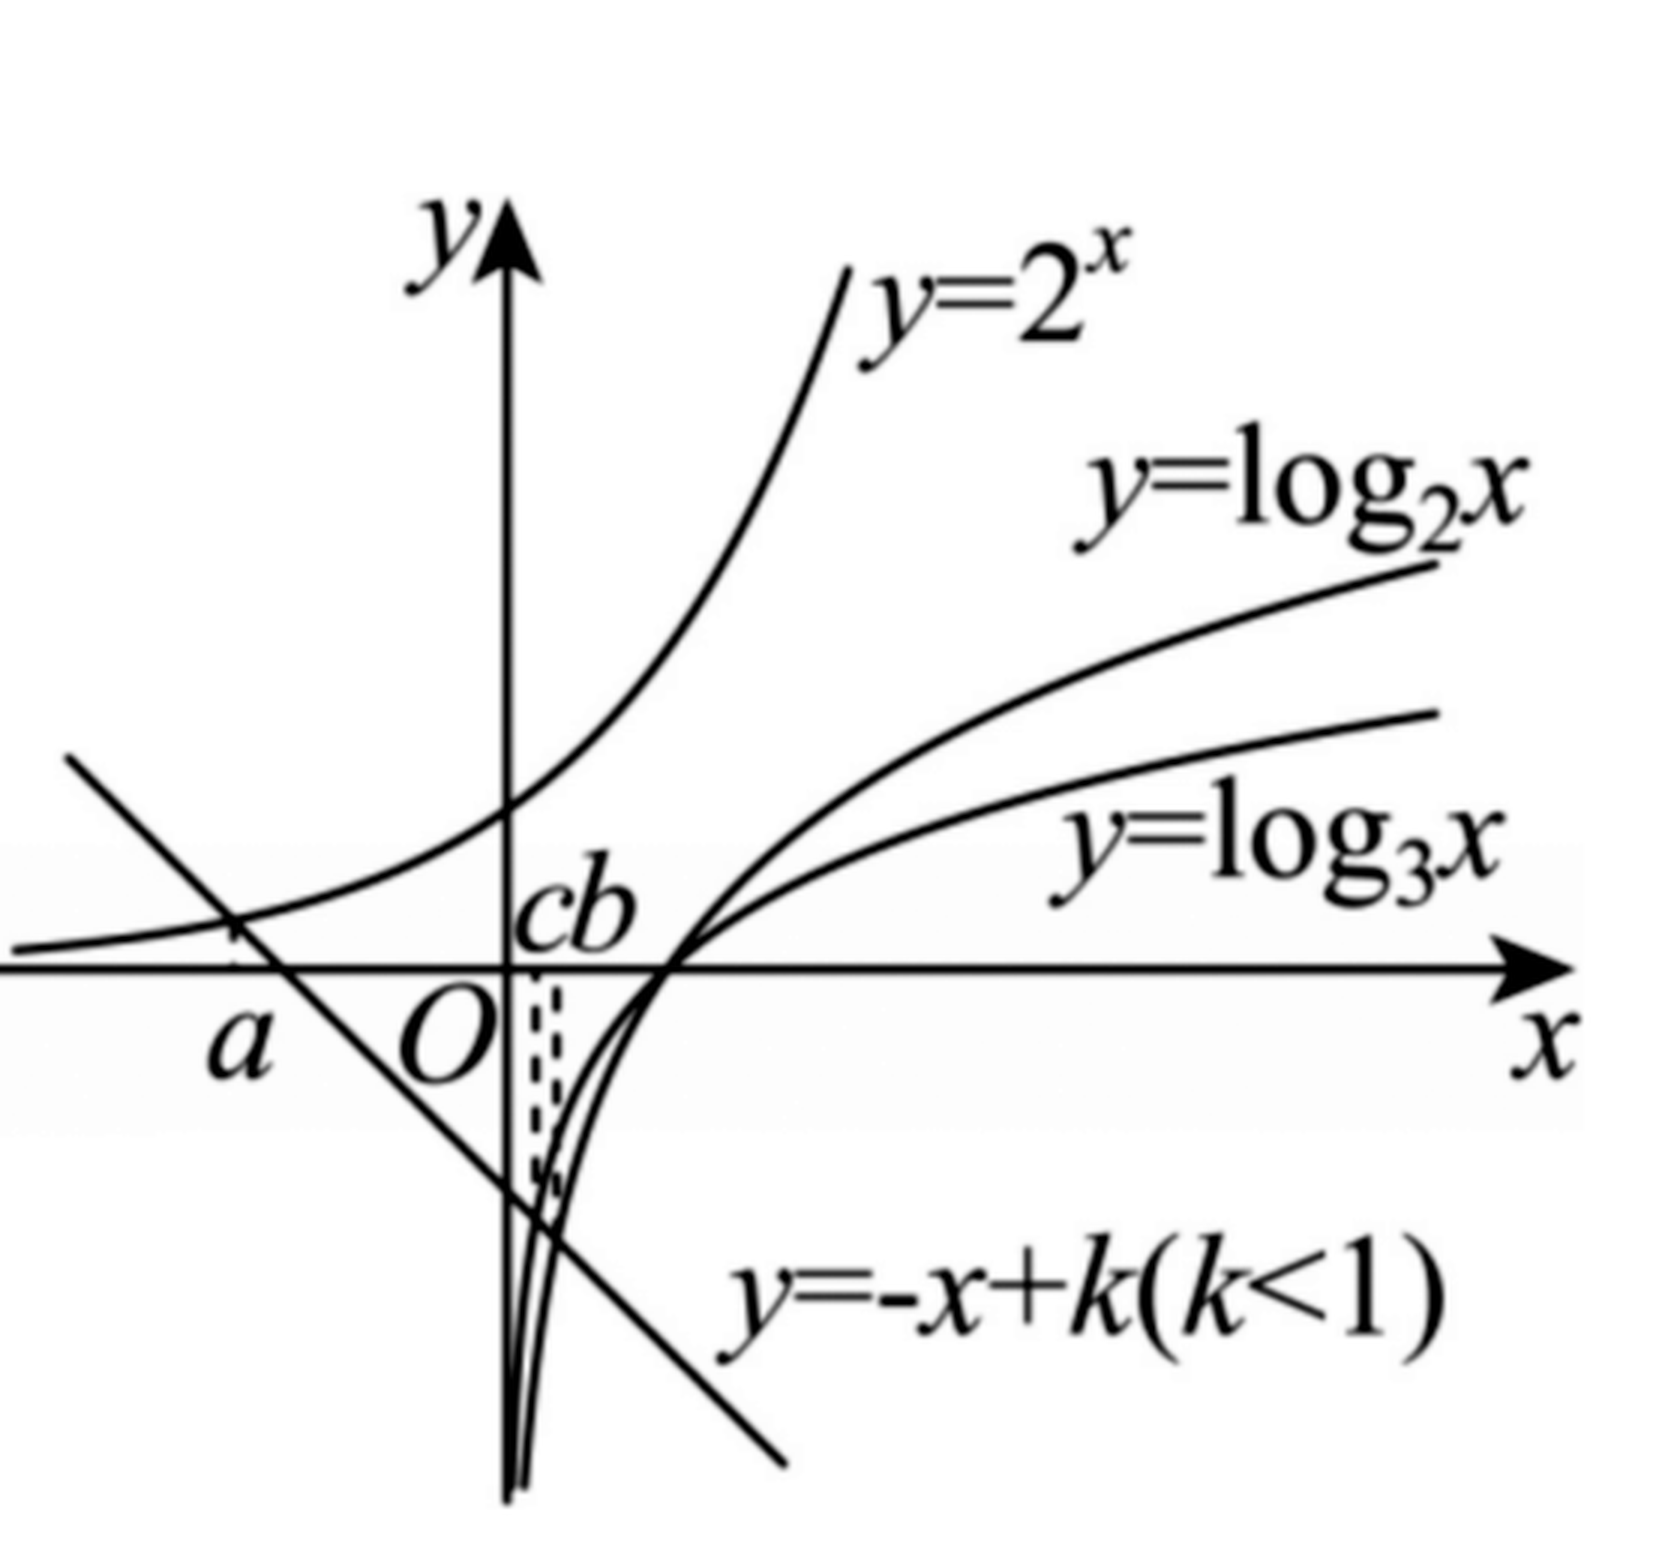
\includegraphics[width=0.52\textwidth]{figures/gao156_q15_curves.png}
\end{center}

\step{如图所示，由图象得 $a<c<b$. 故选 $B$.}
\solend
\fi

% === Q16 === ①② 文本圈数字、"一阶/二阶不动点""稳定点"自定义名词；解析 5 行，故选 A
\item 对定义域为 $I$ 的函数 $y=f(x)$，若存在 $x_0\in I$ 使得 $f(x_0)=x_0$，则称 $x_0$ 是函数 $f(x)$ 的
一阶不动点，简称不动点；若存在 $x_0\in I$ 使得 $f(f(x_0))=x_0$，则称 $x_0$ 是函数 $f(x)$ 的二阶
不动点，简称稳定点. 现有如下两个命题：①存在函数非 $y=x$ 且有无穷多个不动点；②
存在函数有无穷多个稳定点，且这些稳定点不都是不动点. 则\mbox{（\quad）}

\keepwithprev
A. ①成立，②成立\qquad\qquad B. ①成立，②不成立

C. ①不成立，②成立\qquad\qquad D. ①不成立，②不成立

\ifanswer
\solbegin
\step{①取定义在全体实数上的 $f(x)=\lvert x\rvert$，其不动点为一切非负实数，有无穷多个，}
\step{且 $f(-1)=1\ne-1$，①成立.}
\step{②取定义在全体实数上的 $g(x)=-x$，则 $g(g(x))=-(-x)=x$，}
\step{全体实数都是稳定点，而不动点只有 0，②成立.}
\step{故选 $A$.}
\solend
\fi

\end{enumerate}

\bigsec{三、解答题}

\begin{enumerate}
\setcounter{enumi}{16}

% === Q17 === $A\cap B$、$B\cap C$、\varnothing、\mid；解析 6 行
\item 设集合 $A=\{x\mid-1\leqslant x\leqslant2\}$，$B=\{x\mid2m<x<1\}$，$C=\{x\mid x<-1$ 或 $x>2\}$.

(1) 若 $A\cap B=B$，求实数 $m$ 的取值范围；

(2) 若 $B\cap C$ 中只有一个整数，求实数 $m$ 的取值范围.

\ifanswer
\solbegin
\step{(1) 当 $m\geqslant\dfrac12$ 时，$B=\varnothing$，满足 $A\cap B=B$.}
\step{当 $m<\dfrac12$ 时，$A\cap B=B$ 等价于 $2m\geqslant-1$，得 $-\dfrac12\leqslant m<\dfrac12$.}
\step{因此 $m$ 的取值范围为 $\left[-\dfrac12,+\infty\right)$.}
\step{(2) $B\cap C=\{x\mid2m<x<-1\}$，其中只有一个整数时，该整数必为 $-2$.}
\step{包含 $-2$ 且不包含 $-3$，等价于 $-3\leqslant2m<-2$，}
\step{因此 $m$ 的取值范围为 $\left[-\dfrac32,-1\right)$.}
\solend
\fi

% === Q18 === 幂函数 $x^{-\frac13}$、$m\in\R$；解析 12 行，跨 05—06 页
\item 已知幂函数 $f(x)=(3m^2-2m)x^m$（$m\in\R$）在定义域上不单调.

(1) 求函数 $f(x)$ 的解析式；

(2) 若 $f(a+1)<f(-2a+3)$，求实数 $a$ 的取值范围.

\ifanswer
\solbegin
\step{(1) 由幂函数的定义，$3m^2-2m=1$，即 $(3m+1)(m-1)=0$，得 $m=1$ 或 $m=-\dfrac13$.}
\step{当 $m=1$ 时，$f(x)=x$ 在定义域上单调递增，不合题意.}
\step{当 $m=-\dfrac13$ 时，$f(-1)=-1<f(1)=1$，而 $f(1)=1>f(8)=\dfrac12$，}
\step{故 $f(x)$ 在定义域上不单调.}
\step{因此 $f(x)=x^{-\frac13}$，定义域为 $(-\infty,0)\cup(0,+\infty)$.}
\step{(2) 有意义的条件为 $a\ne-1$ 且 $a\ne\dfrac32$.}
\step{当 $a<-1$ 时，$a+1<0<-2a+3$，有 $f(a+1)<0<f(-2a+3)$，}
\step{不等式成立.}
\step{当 $-1<a<\dfrac32$ 时，利用 $f(x)$ 在 $(0,+\infty)$ 上单调递减，}
\step{原不等式等价于 $a+1>-2a+3$，得 $\dfrac23<a<\dfrac32$.}
\step{当 $a>\dfrac32$ 时，$f(a+1)>0>f(-2a+3)$，不等式不成立.}
\step{所以 $a\in(-\infty,-1)\cup\left(\dfrac23,\dfrac32\right)$.}
\solend
\fi

% === Q19 === 两套解法（法一红字 \stepm，法二无标签）；\Delta 与 \subseteq；解析 21 行，跨 06—08 页
\item 已知 $a,c\in\R$，函数 $f(x)=\dfrac{x^2+(3a+1)x+c}{x+a}$.

(1) 若 $a=0$，求函数的定义域，并判断是否存在 $c$ 使得 $y=f(x)$ 图像关于原点对称，说明理由；

(2) 若函数过点 $(1,3)$，且函数 $y=f(x)$ 与 $x$ 轴负半轴有两个不同交点，求此时 $c$ 的值和 $a$ 的取值范围.

\ifanswer
\solbegin
\step{(1) 当 $a=0$ 时，$f(x)=\dfrac{x^2+(3a+1)x+c}{x+a}=\dfrac{x^2+x+c}{x}=x+\dfrac cx+1$，}
\step{故定义域为 $(-\infty,0)\cup(0,+\infty)$；}
\step{若存在实数 $c$，使得函数 $f(x)$ 为奇函数，则必有 $f(x)+f(-x)=0$，}
\step{而 $x+\dfrac cx+1+(-x)+\dfrac c{-x}+1=2\ne0$，}
\step{所以不存在实数 $c$，使得函数 $f(x)$ 为奇函数；}
\step{(2) 函数 $f(x)$ 的图像过点 $(1,3)$，则 $f(1)=\dfrac{1+(3a+1)+c}{1+a}=\dfrac{3a+c+2}{a+1}=3$，}
\step{解得 $c=1$，所以 $f(x)=\dfrac{x^2+(3a+1)x+1}{x+a}$，}
\stepm{法一：}{令 $f(x)=0$，则 $x^2+(3a+1)x+1=0$，此时方程有两不等负根，}
\step{则有 $\begin{cases}\Delta=(3a+1)^2-4>0\\-(3a+1)<0\end{cases}\Rightarrow\begin{cases}a>\dfrac13\text{ 或 }a<-1\\a>-\dfrac13\end{cases}\Rightarrow a>\dfrac13$，}
\step{注意到分母 $x+a\ne0$，则 $x\ne-a$，}
\step{若 $x=-a$ 也是方程 $x^2+(3a+1)x+1=0$ 的解，}
\step{代入方程 $(-a)^2+(3a+1)(-a)+1=0\Rightarrow2a^2+a-1=(a+1)(2a-1)=0$，}
\step{解得 $a=-1$ 或 $a=\dfrac12$，从而 $a\ne\dfrac12$，}
\step{综上，实数 $a$ 的取值范围为 $\left(\dfrac13,\dfrac12\right)\cup\left(\dfrac12,+\infty\right)$.}
\step{令 $g(x)=x^2+(3a+1)x+1$，与 $x$ 轴负半轴有两个交点，}
\step{则 $\begin{cases}-(3a+1)<0\\\Delta=(3a+1)^2-4>0\end{cases}\Rightarrow a>\dfrac13$.}
\step{注意到分母 $x+a\ne0$，则 $x\ne-a$，}
\step{若 $x=-a$ 也是方程 $x^2+(3a+1)x+1=0$ 的解，}
\step{代入方程 $(-a)^2+(3a+1)(-a)+1=0\Rightarrow2a^2+a-1=(a+1)(2a-1)=0$，}
\step{解得 $a=-1$ 或 $a=\dfrac12$，从而 $a\ne\dfrac12$，}
\step{综上，实数 $a$ 的取值范围为 $\left(\dfrac13,\dfrac12\right)\cup\left(\dfrac12,+\infty\right)$.}
\solend
\fi

% === Q20 === $Q$ 常数段 80000 照录；cases 与基本不等式；解析 10 行，跨 08—09 页
\item 某工厂生产某种零件的固定成本为 20000 元，每生产一个零件要增加投入 100 元，已知
总收入 $Q$（单位：元）关于产量 $x$（单位：个）满足函数：$Q=\begin{cases}400x-\dfrac12x^2,&0\leqslant x\leqslant400\\80000,&x>400\end{cases}$.

(1) 将利润 $P$（单位：元）表示为产量 $x$ 的函数；（总收入$=$总成本$+$利润）

(2) 当产量为何值时，零件的单位利润最大？最大单位利润是多少元？（单位利润$=$利润$\div$产量）

\ifanswer
\solbegin
\step{(1) 当 $0\leqslant x\leqslant400$ 时，}
\step{$P(x)=400x-\dfrac12x^2-20000-100x=-\dfrac12x^2+300x-20000$，}
\step{当 $x>400$ 时，$P(x)=80000-100x-20000=60000-100x$，}
\step{故 $P(x)=\begin{cases}-\dfrac12x^2+300x-20000,&0\leqslant x\leqslant400\\60000-100x,&x>400\end{cases}$.}
\step{(2) 设零件的单位利润为 $g(x)$，则 $g(x)=\begin{cases}-\dfrac12x-\dfrac{20000}{x}+300,&0\leqslant x\leqslant400\\\dfrac{60000}{x}-100,&x>400\end{cases}$，}
\step{当 $0\leqslant x\leqslant400$ 时，}
\step{$g(x)=300-\left(\dfrac12x+\dfrac{20000}{x}\right)\leqslant300-2\sqrt{\dfrac x2\cdot\dfrac{20000}{x}}=100$，}
\step{当且仅当 $\dfrac x2=\dfrac{20000}{x}$，即 $x=200$ 时取等号，}
\step{当 $x>400$ 时，$g(x)=\dfrac{60000}{x}-100$，此时无最值，}
\step{故当产量为 200 个，零件的单位利润最大，最大单位利润是 100 元.}
\solend
\fi

% === Q21 === 上升集定义、$D(x_0)=\{d\in\R\mid\cdots\}$、①②③ 文本圈数字、
%            \subseteq 带下划线、$-2^{-x}$；解析 19 行，跨 09—10 页
\item 已知函数 $y=f(x)$ 的定义域为 $\R$. 对任意 $x_0\in\R$，定义集合
$D(x_0)=\{d\in\R\mid f(x_0+d)>f(x_0)\}$，则称 $D(x_0)$ 为函数 $y=f(x)$ 在 $x_0$ 处的上升集.

(1) 若 $f(x)=1-x$，求 $D(-1)$；

(2) 若 $f(x)=\begin{cases}2^x,&x<0\\0,&x=0\\-2^{-x},&x>0\end{cases}$，求 $D(x)$；

(3) 设 $y=f(x)$ 满足：①当 $x<0$ 时，$f(x)=2^x$；②若 $f(x_1)\leqslant f(x_2)$，则
$D(x_2)\subseteq D(x_1)$；③当 $0<x<1$ 时，$f(x)<f(0)$. 证明：$f(0)\geqslant1$.

\ifanswer
\solbegin
\step{(1) $f(-1+d)>f(-1)\Leftrightarrow2-d>2\Leftrightarrow d<0$，所以 $D(-1)=(-\infty,0)$.}
\step{(2) 函数在 $(-\infty,0)$、$(0,+\infty)$ 上分别严格递增，}
\step{且这两个区间上的函数值分别为正、负，$f(0)=0$.}
\step{当 $x<0$ 时，$f(x+d)>f(x)\Leftrightarrow x<x+d<0\Leftrightarrow0<d<-x$，}
\step{当 $x=0$ 时，$f(d)>f(0)\Leftrightarrow d<0$，}
\step{当 $x>0$ 时，$f(x+d)>f(x)\Leftrightarrow x+d\leqslant0$ 或 $x+d>x$}
\step{$\Leftrightarrow d\leqslant-x$ 或 $d>0$，}
\step{因此 $D(x)=\begin{cases}(0,-x),&x<0\\(-\infty,0),&x=0\\(-\infty,-x]\cup(0,+\infty),&x>0\end{cases}$.}
\step{(3) 任取 $a\in(-1,0)$，}
\step{令 $d=-\dfrac a2$，则 $0<d<1$，且 $f(a+d)=2^{\frac a2}>2^a=f(a)$，}
\step{所以 $d\in D(a)$；}
\step{由③，$f(d)<f(0)$，所以 $d\notin D(0)$.}
\step{若 $f(0)\leqslant f(a)$，由②得 $D(a)\subseteq D(0)$，与上述结论矛盾.}
\step{因此，对任意 $a\in(-1,0)$，都有 $f(0)>2^a$.}
\step{特别地 $f(0)>2^{-\frac12}>0$.}
\step{若 $f(0)<1$，取 $a=\dfrac12\log_2 f(0)$，则 $-\dfrac14<a<0$，且}
\step{$2^a=\sqrt{f(0)}>f(0)$，}
\step{与 $f(0)>2^a$ 矛盾.}
\step{所以 $f(0)\geqslant1$.}
\solend
\fi

\end{enumerate}

\end{document}
"
% 紧凑版：xelatex "\def\iscompact{1}% 高一156_大同中学_期中.tex
%   —— 高一上数学"2026-2027 年大同中学高一上期中"（试卷版/答案版/紧凑版）
% 试卷版：xelatex 高一156_大同中学_期中.tex
% 答案版：xelatex "\def\isanswer{1}\input{高一156_大同中学_期中.tex}"
% 紧凑版：xelatex "\def\iscompact{1}\input{高一156_大同中学_期中.tex}"
%
% ① 原始材料：微信公众号"魔都数学加油站"文章，连载"27学年高一156"，原文标题
% "27学年高一156——2026-2027年上海市大同中学高一上期中"；
% 原文链接：https://mp.weixin.qq.com/s/xLtS5tyjCPJIWCIBohwGvw 。
% 正文为 10 张 PNG 页（01/02/03/04/05/06/07/08/09/10 各页分辨率混排
% 2560×3620 与 4762×6735，逐页按各自分辨率裁图核对）。
% 体例：讲评版——填空 3—12（10 题）、选择 13—16（4 题）、解答 17—21（5 题），
% 共 19 题，自第 3 题起编（1、2 未印在本篇）；Q3 只印【答案】、其余 18 题
% 逐题印【解析】（逐题核实，见 ②）。题目、答案、解析均据原图转录；卷面粉红色
% 水印"魔都数学加油站"及公众号页脚未录入。
%
% 卷首标题：原卷印作"2026-2027 年大同中学高一上期中"，年份区间按全稿惯例排 en dash；
% 原卷卷面未印副标题，本稿按同期中卷知识模块口径补出"集合与常用逻辑用语、不等式、函数"。
%
% ② 与原卷的排版差异：
%   ① 原文从第 3 题起，本稿保留原题号；共 19 题三节，解答题 5 题到 21；
%   ② 混合体例：第 3 题只印【答案】、无【解析】，按 高一140 第 5 题／高一145
%      第 3 题／高一151 第 7 题成例另提 \ans{}、不补造解析；其余 18 题印
%      【解析】、用 \solbegin…\solend；四道选择题答案在解析末句"故选 C／C／B／A"
%      （逐个放大复核）、括号 \mbox{（\quad）} 留空、不另提 \ans{}；答案版
%      【答案】/【解析】标记数 = 19 = 全卷题数（1 个 \ans ＋ 18 个 \solbegin）；
%   ③ 原卷卷面未印副标题，本稿按知识模块口径补出；
%   ④ 原卷填空横线按全稿惯例排 \blankline[4.4em]；选择题括号排 \mbox{（\quad）}、
%      选项段前按惯例各加 \keepwithprev；解答题不留作答区、不加 \anspace
%      （原卷为讲评版，109—113 起全稿不用 \anspace）；
%   ⑤ 数集：Q3"$x\in\R$"、Q18"$m\in\R$"、Q19"$a,c\in\R$"、Q21"定义域为 \R"
%      "任意 $x_0\in\R$""$d\in\R$"原卷印正体粗体 R，按全稿惯例归一 \R；
%      绝对值排 \lvert…\rvert（Q11 $\lvert2^x-1\rvert$、Q16 $\lvert x\rvert$），
%      集合描述竖线排 \mid（Q17 $A=\{x\mid\cdots\}$、Q21 $D(x_0)=\{d\in\R\mid\cdots\}$），
%      空集 \varnothing（Q17"$B=\varnothing$"），不等号按全稿惯例排 \leqslant／\geqslant；
%   ⑥ 子集符号逐处照录不统一：Q21 (3) 题干"$D(x_2)\subseteq D(x_1)$"与解析
%      "$D(a)\subseteq D(0)$"均印带下划线 ⊆，照录 \subseteq；本卷无单线 ⊂ 用例；
%   ⑦ 判别式：Q19 两套解法"$\Delta=(3a+1)^2-4>0$"印等腰偏高 \Delta，照录 \Delta；
%      本卷无扁三角 \triangle 用例；
%   ⑧ 红字照录为黑体：Q19 (2) 解析第一套解法行首"法一："原卷排**红色加粗**，
%      按 高一53 成例排 \stepm{法一：}{…}（加粗着色、不改黑色基调），全库无红字
%      排字先例、本稿不引入红色定义，文件头注明；第二套解法原卷直接以
%      "令 $g(x)=x^2+(3a+1)x+1$，与 $x$ 轴负半轴有两个交点，"另起，
%      **未印"法二："标签**（逐页像素级复核：07 页仅 1437—1475 一处红字，
%      08 页无红字），照录为普通 \step、不补造标签；
%   ⑨ 文本模式圈数字逐处照录：Q12 解析 ①② 两情形、Q16 两则命题与四个选项及
%      解析的 ①②、Q21 (3) 三条件 ①②③ 与解析"由③""由②"，均为印刷圈数字
%      （非 \textcircled、非数学模式），计入圈数字实测；
%   ⑩ 自定义名词照录：Q16"一阶不动点，简称不动点""二阶不动点，简称稳定点"、
%      Q21"上升集"；Q16 题干"存在函数非 $y=x$ 且有无穷多个不动点"照录；
%   ⑪ 中文弯引号照录：Q3""存在 $x\in\R$，$x^3-1\leqslant0$" 否定形式为"、
%      Q13"使"$\dfrac{x+1}{1-x}\geqslant0$"成立的必要不充分条件是"；
%      注释里一律 ASCII 引号；数学式内 CJK 用 \text{}（Q19 cases 内"或"）；
%   ⑫ 半角逗号在数学组之间是全稿惯例、非笔误，逐处照录（$a,c$、$x,y$、$a,b$
%      之类）；行末西文句点 ASCII `.`；行中全角逗号／顿号照录；
%   ⑬ 复杂式照录别简化：Q6 $\left(\dfrac{1}{\sqrt a}\right)^{\frac27}\cdot\sqrt[7]{a^3}$
%      与解析 $a^{\frac{12}{7}-\frac17+\frac37}$、Q8 $2\sqrt4+5=9$（$\sqrt4$ 未化简）、
%      Q9 $\left(\sqrt x+\dfrac{1}{\sqrt x}\right)^3$、Q12 $\dfrac{4a-(2-a)^2}{4a}$、
%      Q18 $f(8)=\dfrac12$、Q19 $2a^2+a-1=(a+1)(2a-1)=0$、Q20 $Q$ 的常数段
%      $80000$（不是 $80000-100x$）与 $2\sqrt{\dfrac x2\cdot\dfrac{20000}{x}}$、
%      Q21 $f(a+d)=2^{\frac a2}>2^a=f(a)$ 与 $2^a=\sqrt{f(0)}>f(0)$ 等；
%      \left…\right 不得拆到不同 $…$ 组（Q5 $\left(0,\dfrac12\right)$、
%      Q12 $\left[0,4+2\sqrt3\right)$、Q17 $\left[-\dfrac12,+\infty\right)$、
%      Q19 $\left(\dfrac13,\dfrac12\right)\cup\left(\dfrac12,+\infty\right)$、
%      Q20 $\left(\dfrac12x+\dfrac{20000}{x}\right)$ 等）；cases 块整体算一个印刷行；
%   ⑭ 一条 \step = 原卷解析的一个印刷行；别并折行、别拆行。跨页续印按题合并
%      （Q6 的 01 页上下题干重复印、Q8 的 01—02 页、Q12 的 02—03 页、
%      Q15 的 04 页上下、Q16 的 04—05 页、Q17 的 05 页上下、Q18 的 05—06 页、
%      Q19 的 06—08 页、Q20 的 08—09 页、Q21 的 09—10 页）；
%      跨半页重叠行（Q12 的"②若 …"、Q18 的"原不等式等价于 …"、
%      Q20 的"【解析】(1) 当 $0\leqslant x\leqslant400$ 时，"、Q21 的
%      "【解析】(1) $f(-1+d)>f(-1)\cdots$"与"与 $f(0)>2^a$ 矛盾."）
%      只算一个印刷行；
%   ⑮ 配图：全卷 3 组（逐页通读 10 页确认）——
%      · Q14 题干 S-t 梯形图（03 页右下，离家距离 S 对行走时间 t），题目配图、
%        三版都出，裁 figures/gao156_q14_st.png；
%      · Q14 四幅路线选项（04 页上部，A/B/C/D 四幅横排、C 为以家为圆心的圆弧），
%        题目配图、三版都出，合并成一张，裁 figures/gao156_q14_opts.png；
%      · Q15 解析内曲线交点图（04 页右下，$y=2^x$、$y=\log_2x$、$y=\log_3x$
%        与 $y=-x+k$），仅答案版出，裁 figures/gao156_q15_curves.png；
%      3 图均取自原卷截图，去粉色水印、去色、3×~4× LANCZOS 放大；
%      Q14 题干"题干＋两图"整块用 \needvspace 守卫推走（守卫放 \item 之前，
%      见 高一154 Q15／高一136 Q13 成例）；Q15 解析内图放 \ifanswer 内
%      \solbegin…\solend 的两 \step 之间（高一108 第 6 题／高一154 附加题 2 成例）；
%      其余各页逐页确认无其它题目配图、无解析配图、无表格；10 页下半仅水印、无正文。
%
% ③ 行数复核：一条 \step = 原卷解析的一个印刷行，cases 块作一个印刷行计。
%   逐题数（主会话逐页核对定稿）：Q3：0（只印【答案】、提 \ans{}，不计入 \step 账）；
%   Q4：1；Q5：1；Q6：1；Q7：1；Q8：3；Q9：2；Q10：2；Q11：5；Q12：12；
%   Q13：3；Q14：3；Q15：4；Q16：5；Q17：6；Q18：12；Q19：21；Q20：10；Q21：19。
%   合计 111 行（110 条 \step ＋ 1 条 \stepm），与原卷逐题印刷行相等。
%   全卷 19 题：Q3 一处 \ans{} ＋ 其余 18 题设 \solbegin…\solend，
%   答案版【答案】/【解析】标记数 = 19 = 全卷题数。
%
% ④ 页码分布（供回原图复核）：
%   卷首标题＋"一、填空题"＋Q3 题干＋【答案】、Q4 题干＋解析 1 行、
%   Q5 题干＋解析 1 行、Q6 题干首行在 01 页上半；
%   Q6 题干（重复印）＋解析 1 行、Q7 题干＋解析 1 行、Q8 题干＋解析前 2 行
%   在 01 页下半；Q8 解析末行、Q9 题干＋解析 2 行、Q10 题干＋解析 2 行、
%   Q11 题干首行在 02 页上半；Q11 题干（重复印）＋解析 5 行、
%   Q12 题干＋解析首行在 02 页下半；Q12 解析中 9 行在 03 页上半；
%   Q12 解析末 2 行＋"二、选择题"标题＋Q13 题干＋选项＋解析 3 行＋
%   Q14 题干首行在 03 页下半；Q14 题干续行＋四幅选项图＋解析 3 行＋
%   Q15 题干＋选项＋解析前 2 行＋Q16 题干在 04 页上半；
%   Q15 解析后 2 行＋曲线图＋Q16 选项＋解析前 2 行在 04 页下半；
%   Q16 解析后 3 行＋"三、解答题"标题＋Q17 题干＋两问＋解析 (1) 3 行
%   在 05 页上半；Q17 解析 (2) 3 行＋Q18 题干＋两问＋解析 (1) 首 2 行
%   在 05 页下半；Q18 解析 (1)(2) 中 8 行在 06 页上半；Q18 解析末 2 行＋
%   Q19 题干＋两问＋解析 (1) 首行在 06 页下半；Q19 解析 (1) 后 4 行＋
%   (2) 前 2 行＋法一 2 行在 07 页上半；法一后 5 行＋法二前 3 行在 07 页下半；
%   法二后 4 行＋Q20 题干＋两问＋解析 (1) 首行在 08 页上半；
%   Q20 解析 (1) 后 3 行＋(2) 前 5 行在 08 页下半；Q20 解析 (2) 末 2 行＋
%   Q21 题干＋三问＋解析 (1) 首行在 09 页上半；Q21 解析 (1)（重复印）＋
%   (2) 8 行＋(3) 首行在 09 页下半；Q21 (3) 解析中 8 行在 10 页上半；
%   Q21 (3) 末 2 行在 10 页下半。本稿按题连排，不丢行、不并折行；
%   全卷末题为第 21 题，无附加题节。
%
\documentclass[a4paper,11pt]{article}
\usepackage{common}

\begin{document}

\examtitlest[3]{2026--2027 年大同中学高一上期中}{集合与常用逻辑用语、不等式、函数}

\bigsec{一、填空题}

\begin{enumerate}
\setcounter{enumi}{2}

% === Q3 === 只印【答案】、无【解析】；R 正体粗体 \R；中文弯引号照录
\item “存在 $x\in\R$，$x^3-1\leqslant0$” 否定形式为\blankline[4.4em].

\ifanswer
\ans{对任意 $x\in\R$，$x^3-1>0$}
\fi

% === Q4 === 解析 1 行
\item 若实数 $a>0$ 且 $a\ne1$，函数 $y=a^{x-3}+1$ 的图像恒过定点 $P$，则点 $P$ 的坐标为\blankline[4.4em].

\ifanswer
\solbegin
\step{当 $x=3$ 时，$y=a^0+1=2$，与 $a$ 无关，所以定点为 $P(3,2)$.}
\solend
\fi

% === Q5 === 解析 1 行
\item 函数 $y=\dfrac{1}{3^x+2}$ 的值域是\blankline[4.4em].

\ifanswer
\solbegin
\step{$3^x\in(0,+\infty)$，因此 $3^x+2\in(2,+\infty)$，值域为 $\left(0,\dfrac12\right)$.}
\solend
\fi

% === Q6 === 根式嵌套照录；解析 1 行；题干跨 01 页上下重复印
\item 已知 $a>0$，化简 $a^{\frac{12}{7}}\cdot\left(\dfrac{1}{\sqrt a}\right)^{\frac27}\cdot\sqrt[7]{a^3}=$\blankline[4.4em].

\ifanswer
\solbegin
\step{原式 $=a^{\frac{12}{7}}\cdot a^{-\frac17}\cdot a^{\frac37}=a^{\frac{12}{7}-\frac17+\frac37}=a^2$.}
\solend
\fi

% === Q7 === 换底公式；解析 1 行
\item 已知 $\log_5 3=a$，用 $a$ 的代数式表示 $\log_{15}125=$\blankline[4.4em].

\ifanswer
\solbegin
\step{$\log_{15}125=\dfrac{\log_5 125}{\log_5 15}=\dfrac{3}{1+\log_5 3}=\dfrac{3}{1+a}$.}
\solend
\fi

% === Q8 === 基本不等式，$\sqrt4$ 照录未化简；解析 3 行，跨 01—02 页
\item 已知 $x>0$，$y>0$，且 $4x+y=xy$，则 $x+y$ 的最小值为\blankline[4.4em].

\ifanswer
\solbegin
\step{由 $4x+y=xy$，得 $\dfrac4y+\dfrac1x=1$，}
\step{则 $x+y=(x+y)\left(\dfrac4y+\dfrac1x\right)=\dfrac{4x}{y}+\dfrac yx+1+4\geqslant2\sqrt4+5=9$，}
\step{当且仅当 $\dfrac{4x}{y}=\dfrac yx$，即 $x=3$，$y=6$ 时取等号，故最小值为 9.}
\solend
\fi

% === Q9 === 解析 2 行
\item 已知 $x^{-1}+x=7$（$x>0$），则 $x^{\frac32}+x^{-\frac32}$ 的值为\blankline[4.4em].

\ifanswer
\solbegin
\step{$x>0$，有 $\sqrt x+\dfrac{1}{\sqrt x}=\sqrt{x+\dfrac1x+2}=3$，}
\step{所以 $x^{\frac32}+x^{-\frac32}=\left(\sqrt x+\dfrac{1}{\sqrt x}\right)^3-3\left(\sqrt x+\dfrac{1}{\sqrt x}\right)=27-9=18$.}
\solend
\fi

% === Q10 === $x_{\min}$；解析 2 行
\item 已知不等式 $x>\dfrac{2a+1}{a-1}$ 对任意的 $x\in[1,2]$ 恒成立，则实数 $a$ 的取值范围是\blankline[4.4em].

\ifanswer
\solbegin
\step{不等式 $x>\dfrac{2a+1}{a-1}$ 对任意的 $x\in[1,2]$ 恒成立，得 $\dfrac{2a+1}{a-1}<x_{\min}=1$，}
\step{即有 $\dfrac{a+2}{a-1}<0$，解得 $-2<a<1$，则实数 $a$ 的取值范围是 $(-2,1)$.}
\solend
\fi

% === Q11 === 分段函数 cases 与绝对值 \lvert…\rvert；解析 5 行
\item 已知函数 $f(x)=\begin{cases}\lvert2^x-1\rvert-a,&x\leqslant2\\\dfrac{3}{x-1}-a,&x>2\end{cases}$，若函数 $y=f(x)$ 图像与 $x$ 轴有三个不同交点，则实数 $a$ 的取值范围是\blankline[4.4em].

\ifanswer
\solbegin
\step{令 $g(x)=f(x)+a$.}
\step{在 $(-\infty,0)$、$[0,2]$、$(2,+\infty)$ 上，$g(x)$ 均严格单调，}
\step{值域依次为 $(0,1)$、$[0,3]$、$(0,3)$.}
\step{每段至多有一个交点，因而恰有三个不同交点，}
\step{当且仅当 $a\in(0,1)\cap[0,3]\cap(0,3)=(0,1)$.}
\solend
\fi

% === Q12 === ①② 文本圈数字、对称轴与最小值式照录；解析 12 行，跨 02—03 页
\item 已知函数 $f(x)=ax^2-(2-a)x+1$，$g(x)=x$，若对于任意实数 $x$，$f(x)$ 与 $g(x)$ 至少有一个为正数，则实数 $a$ 的取值范围是\blankline[4.4em].

\ifanswer
\solbegin
\step{当 $x>0$ 时，$g(x)>0$；当 $x<0$ 时，$g(x)<0$；}
\step{当 $x=0$ 时，$f(0)=1>0$；}
\step{因为对于任意实数 $x$，$f(x)$ 与 $g(x)$ 至少有一个为正数，}
\step{当 $x<0$ 时，因为 $g(x)<0$，所以 $f(x)=ax^2-(2-a)x+1>0$ 恒成立，}
\step{当 $a<0$ 时，显然不成立，}
\step{当 $a=0$ 时，$f(x)=-2x+1>0$，对 $x<0$ 时恒成立，满足题意，}
\step{当 $a>0$ 时，函数图象开口向上，对称轴 $x=\dfrac{2-a}{2a}$，}
\step{①若 $\dfrac{2-a}{2a}\geqslant0$，即 $0<a\leqslant2$ 时，函数 $f(x)$ 在 $(-\infty,0)$ 上严格减，$f(0)=1$，}
\step{故 $f(x)>0$ 对 $x<0$ 时恒成立，满足题意；}
\step{②若 $\dfrac{2-a}{2a}<0$，即 $a>2$ 时，$f(x)_{\min}=f\left(\dfrac{2-a}{2a}\right)=\dfrac{4a-(2-a)^2}{4a}>0$，}
\step{解得 $4-2\sqrt3<a<4+2\sqrt3$，所以 $2<a<4+2\sqrt3$.}
\step{综上，$0\leqslant a<4+2\sqrt3$，故实数 $a$ 的取值范围是 $\left[0,4+2\sqrt3\right)$.}
\solend
\fi

\end{enumerate}

\bigsec{二、选择题}

\begin{enumerate}
\setcounter{enumi}{12}

% === Q13 === 必要不充分条件；cases 块；解析 3 行，故选 C
\item 使 “$\dfrac{x+1}{1-x}\geqslant0$” 成立的必要不充分条件是\mbox{（\quad）}

\keepwithprev
A. $-1\leqslant x<1$\qquad B. $x\leqslant-1$ 或 $x>1$\qquad C. $-1\leqslant x\leqslant1$\qquad D. $x\leqslant-1$ 或 $x\geqslant0$

\ifanswer
\solbegin
\step{由不等式 $\dfrac{x+1}{1-x}\geqslant0$ 得 $\begin{cases}(x+1)(1-x)\geqslant0\\1-x\ne0\end{cases}$，解得 $-1\leqslant x<1$，}
\step{由题意结合选项，$-1\leqslant x<1\Rightarrow-1\leqslant x\leqslant1$ 成立，反之不成立，}
\step{所以 $-1\leqslant x\leqslant1$ 是 $\dfrac{x+1}{1-x}\geqslant0$ 成立的必要不充分条件. 故选 $C$.}
\solend
\fi

% === Q14 === 题干 S-t 图＋四幅路线选项（题目配图，三版都出）；守卫放 \item 之前；解析 3 行，故选 C
\needvspace{9cm}
\item 如图是王老师锻炼时所走的离家距离（$S$）与行走时间（$t$）之间的函数关系图，若
用黑点表示王老师家的位置，则王老师行走的路线可能是\mbox{（\quad）}

\begin{center}
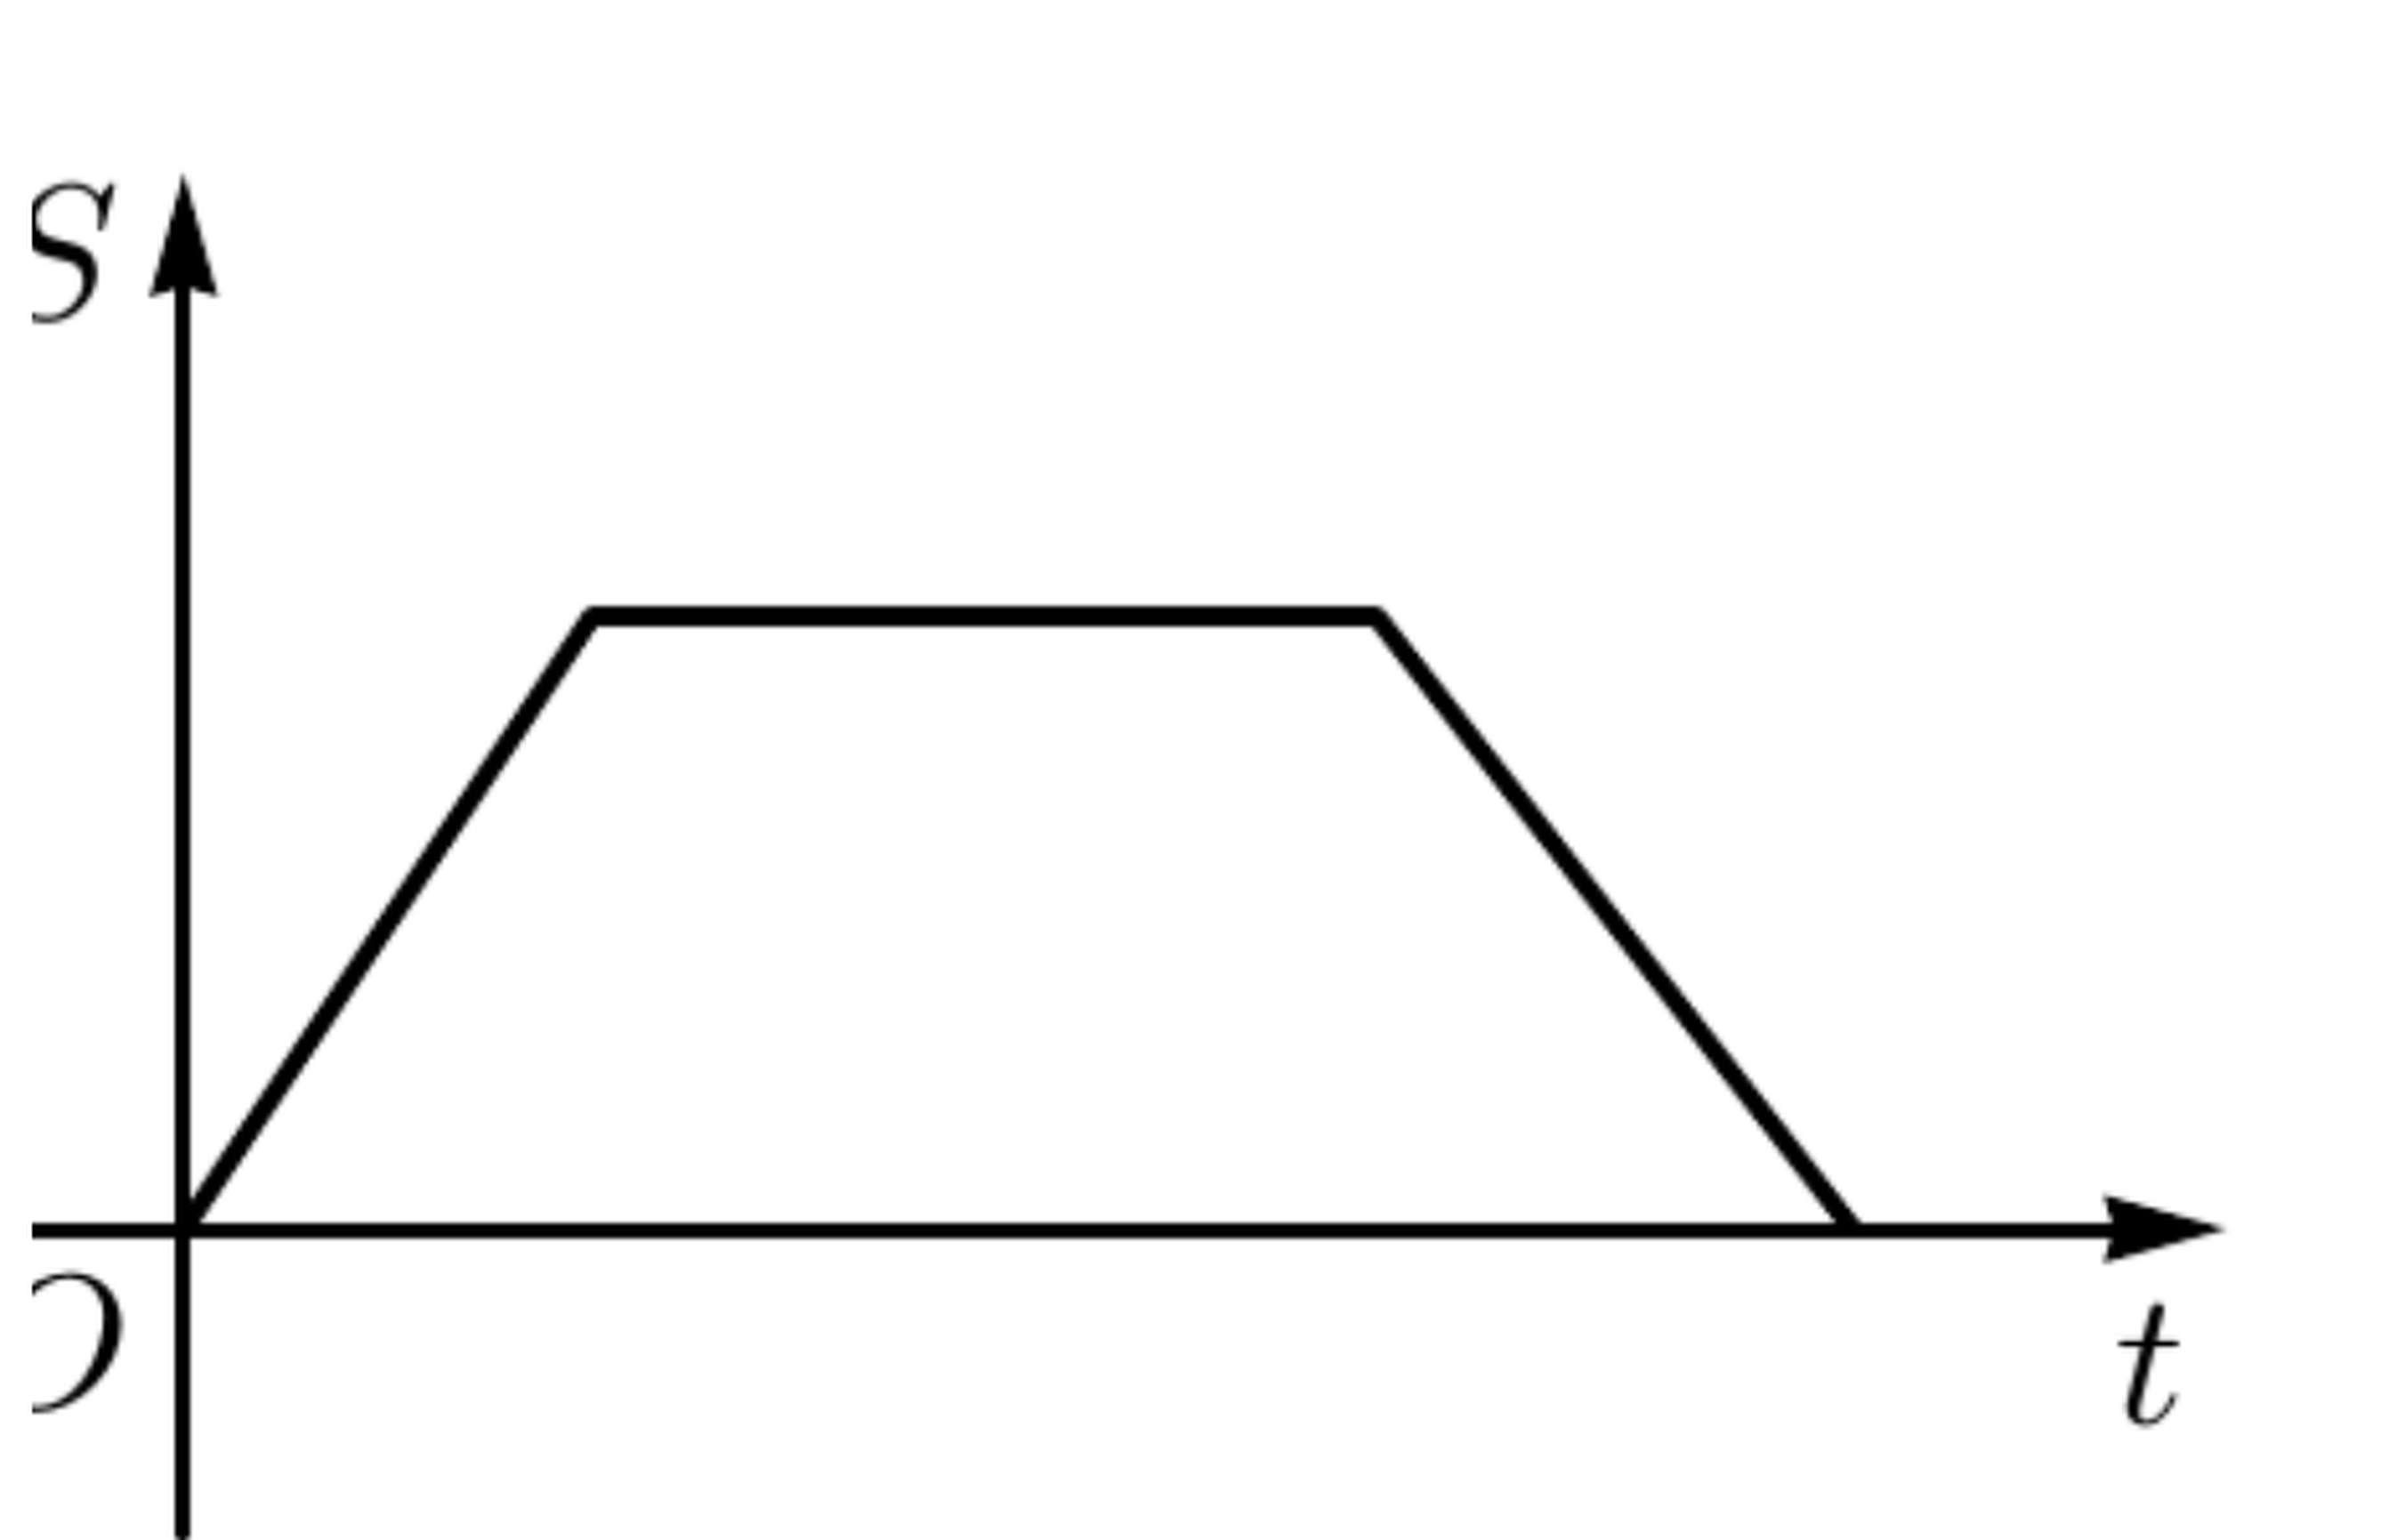
\includegraphics[width=0.34\textwidth]{figures/gao156_q14_st.png}
\end{center}

\keepwithprev
\begin{center}
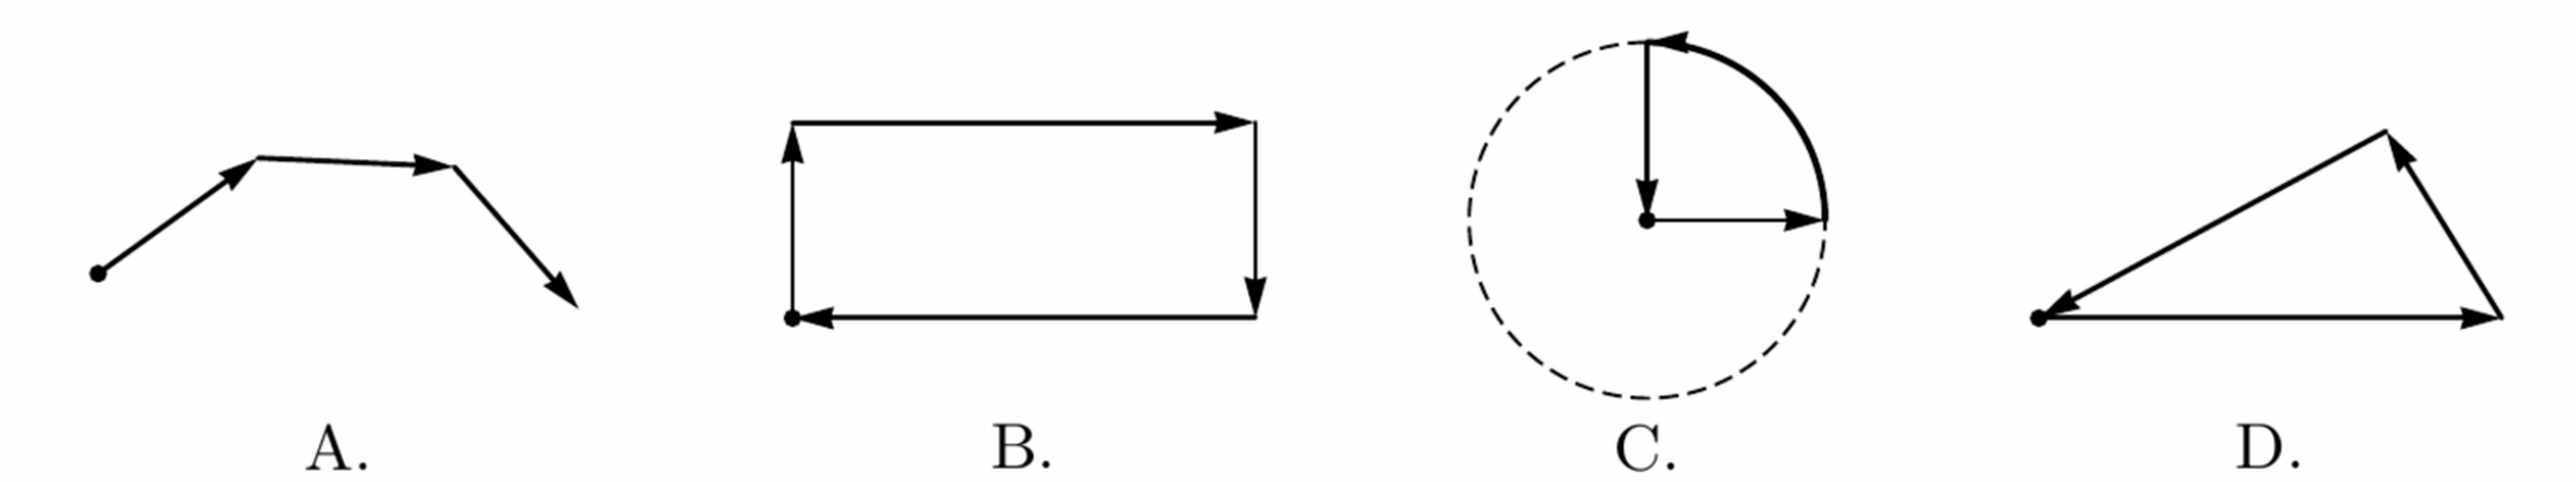
\includegraphics[width=0.86\textwidth]{figures/gao156_q14_opts.png}
\end{center}

\ifanswer
\solbegin
\step{由王老师锻炼时所走的离家距离（$S$）与行走时间（$t$）之间的函数关系图，}
\step{得在中间一段时间里，他到家的距离为定值，}
\step{故他所走的路程是一段以家为圆心的圆弧，故选 $C$.}
\solend
\fi

% === Q15 === 解析内曲线交点图（仅答案版出）；解析 4 行，故选 B
\item 已知 $a+2^a=b+\log_2 b=c+\log_3 c=k$，若 $k<1$，则\mbox{（\quad）}

\keepwithprev
A. $c<a<b$\qquad B. $a<c<b$\qquad C. $b<a<c$\qquad D. $a<b<c$

\ifanswer
\solbegin
\step{因为 $a+2^a=b+\log_2 b=c+\log_3 c=k$，}
\step{所以 $2^a=-a+k$，$\log_2 b=-b+k$，$\log_3 c=-c+k$，其中 $k<1$；}
\step{分别作出 $y=2^x$，$y=\log_2 x$，$y=\log_3 x$ 和 $y=-x+k$ 的图象，}

\begin{center}
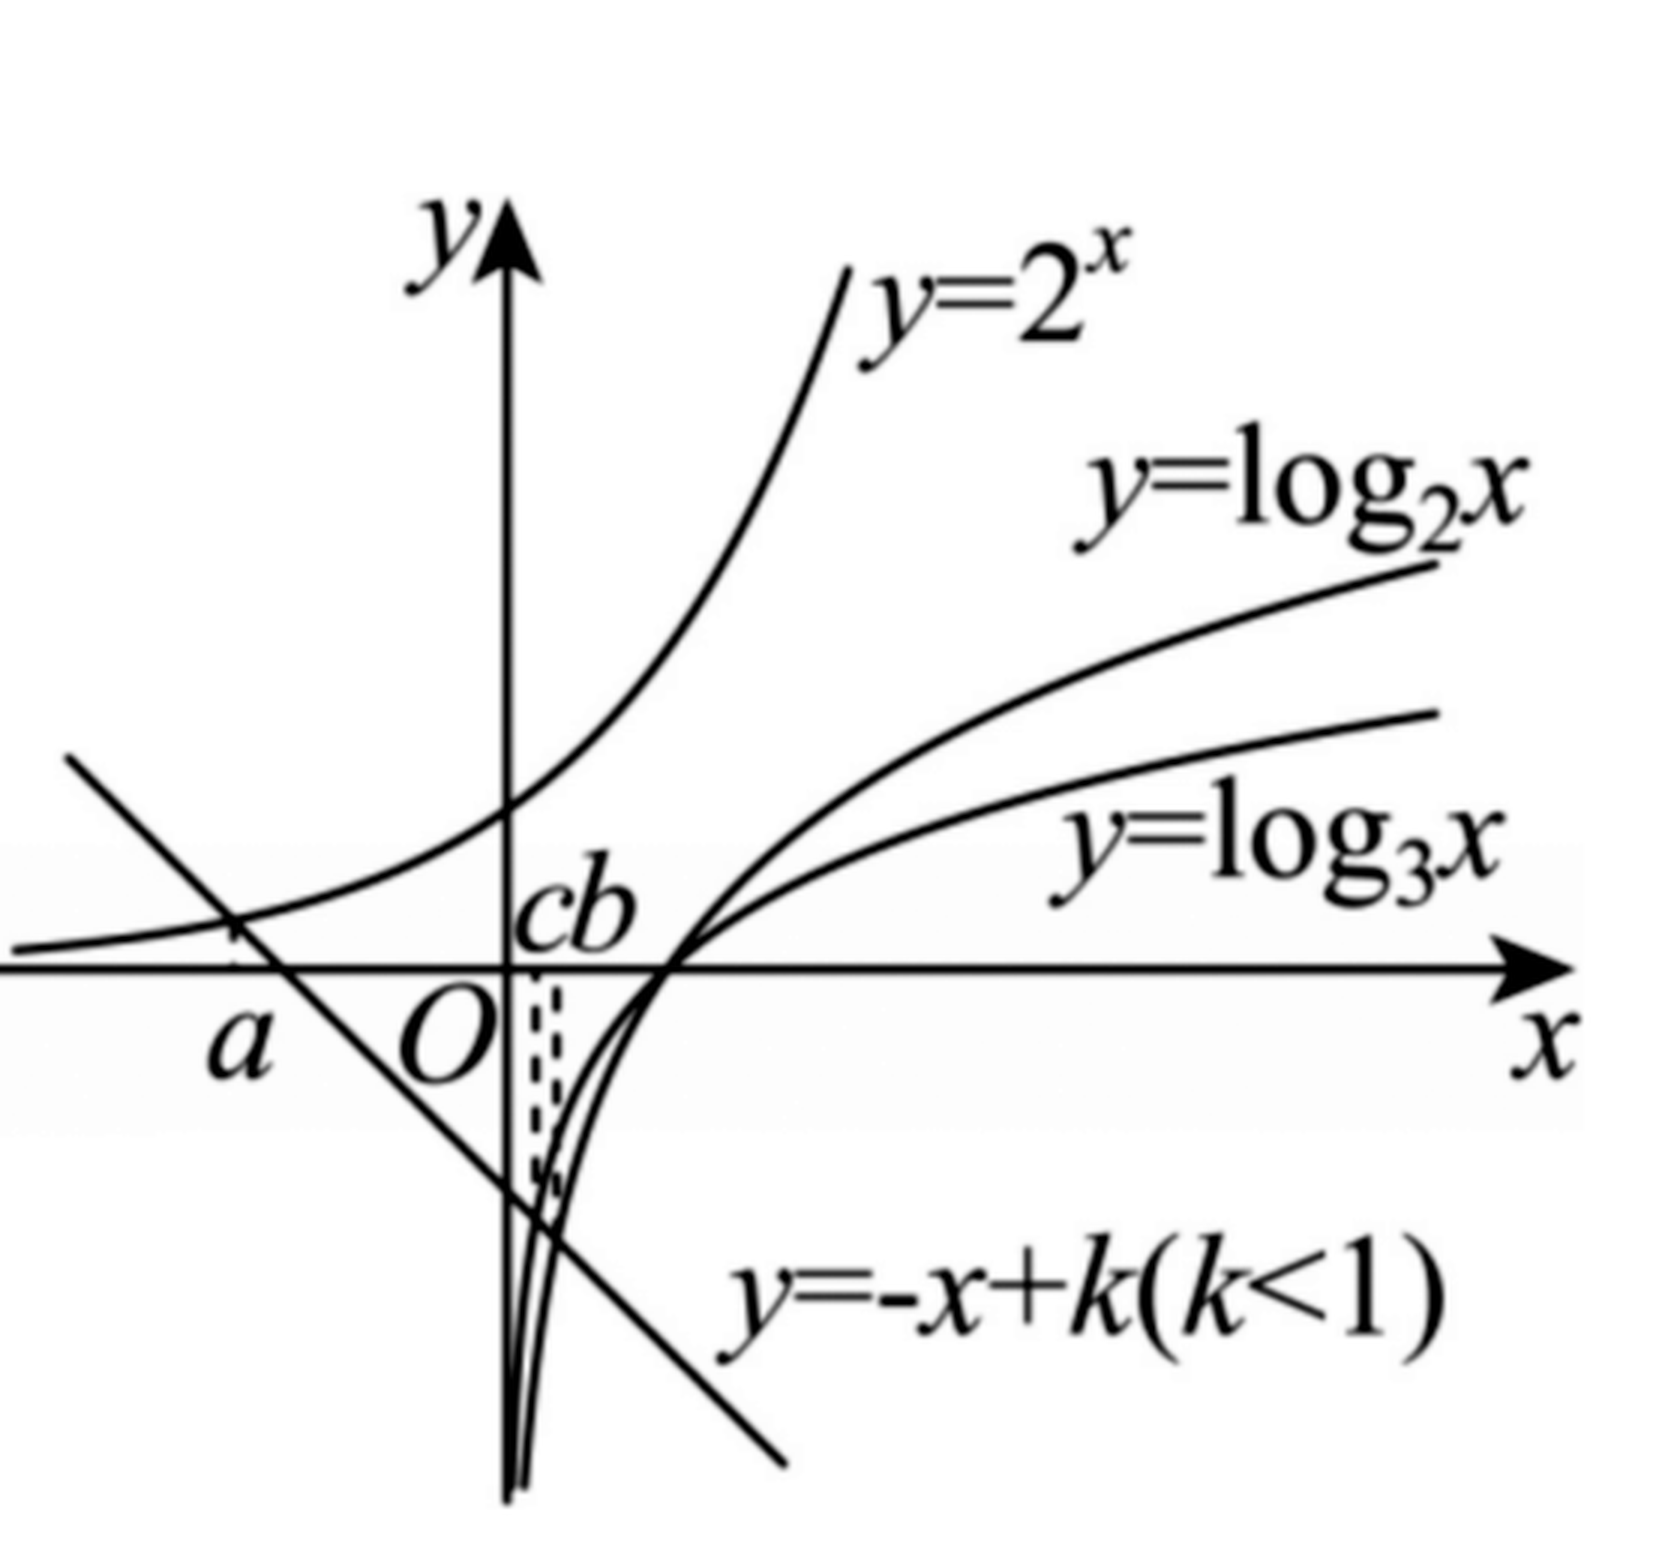
\includegraphics[width=0.52\textwidth]{figures/gao156_q15_curves.png}
\end{center}

\step{如图所示，由图象得 $a<c<b$. 故选 $B$.}
\solend
\fi

% === Q16 === ①② 文本圈数字、"一阶/二阶不动点""稳定点"自定义名词；解析 5 行，故选 A
\item 对定义域为 $I$ 的函数 $y=f(x)$，若存在 $x_0\in I$ 使得 $f(x_0)=x_0$，则称 $x_0$ 是函数 $f(x)$ 的
一阶不动点，简称不动点；若存在 $x_0\in I$ 使得 $f(f(x_0))=x_0$，则称 $x_0$ 是函数 $f(x)$ 的二阶
不动点，简称稳定点. 现有如下两个命题：①存在函数非 $y=x$ 且有无穷多个不动点；②
存在函数有无穷多个稳定点，且这些稳定点不都是不动点. 则\mbox{（\quad）}

\keepwithprev
A. ①成立，②成立\qquad\qquad B. ①成立，②不成立

C. ①不成立，②成立\qquad\qquad D. ①不成立，②不成立

\ifanswer
\solbegin
\step{①取定义在全体实数上的 $f(x)=\lvert x\rvert$，其不动点为一切非负实数，有无穷多个，}
\step{且 $f(-1)=1\ne-1$，①成立.}
\step{②取定义在全体实数上的 $g(x)=-x$，则 $g(g(x))=-(-x)=x$，}
\step{全体实数都是稳定点，而不动点只有 0，②成立.}
\step{故选 $A$.}
\solend
\fi

\end{enumerate}

\bigsec{三、解答题}

\begin{enumerate}
\setcounter{enumi}{16}

% === Q17 === $A\cap B$、$B\cap C$、\varnothing、\mid；解析 6 行
\item 设集合 $A=\{x\mid-1\leqslant x\leqslant2\}$，$B=\{x\mid2m<x<1\}$，$C=\{x\mid x<-1$ 或 $x>2\}$.

(1) 若 $A\cap B=B$，求实数 $m$ 的取值范围；

(2) 若 $B\cap C$ 中只有一个整数，求实数 $m$ 的取值范围.

\ifanswer
\solbegin
\step{(1) 当 $m\geqslant\dfrac12$ 时，$B=\varnothing$，满足 $A\cap B=B$.}
\step{当 $m<\dfrac12$ 时，$A\cap B=B$ 等价于 $2m\geqslant-1$，得 $-\dfrac12\leqslant m<\dfrac12$.}
\step{因此 $m$ 的取值范围为 $\left[-\dfrac12,+\infty\right)$.}
\step{(2) $B\cap C=\{x\mid2m<x<-1\}$，其中只有一个整数时，该整数必为 $-2$.}
\step{包含 $-2$ 且不包含 $-3$，等价于 $-3\leqslant2m<-2$，}
\step{因此 $m$ 的取值范围为 $\left[-\dfrac32,-1\right)$.}
\solend
\fi

% === Q18 === 幂函数 $x^{-\frac13}$、$m\in\R$；解析 12 行，跨 05—06 页
\item 已知幂函数 $f(x)=(3m^2-2m)x^m$（$m\in\R$）在定义域上不单调.

(1) 求函数 $f(x)$ 的解析式；

(2) 若 $f(a+1)<f(-2a+3)$，求实数 $a$ 的取值范围.

\ifanswer
\solbegin
\step{(1) 由幂函数的定义，$3m^2-2m=1$，即 $(3m+1)(m-1)=0$，得 $m=1$ 或 $m=-\dfrac13$.}
\step{当 $m=1$ 时，$f(x)=x$ 在定义域上单调递增，不合题意.}
\step{当 $m=-\dfrac13$ 时，$f(-1)=-1<f(1)=1$，而 $f(1)=1>f(8)=\dfrac12$，}
\step{故 $f(x)$ 在定义域上不单调.}
\step{因此 $f(x)=x^{-\frac13}$，定义域为 $(-\infty,0)\cup(0,+\infty)$.}
\step{(2) 有意义的条件为 $a\ne-1$ 且 $a\ne\dfrac32$.}
\step{当 $a<-1$ 时，$a+1<0<-2a+3$，有 $f(a+1)<0<f(-2a+3)$，}
\step{不等式成立.}
\step{当 $-1<a<\dfrac32$ 时，利用 $f(x)$ 在 $(0,+\infty)$ 上单调递减，}
\step{原不等式等价于 $a+1>-2a+3$，得 $\dfrac23<a<\dfrac32$.}
\step{当 $a>\dfrac32$ 时，$f(a+1)>0>f(-2a+3)$，不等式不成立.}
\step{所以 $a\in(-\infty,-1)\cup\left(\dfrac23,\dfrac32\right)$.}
\solend
\fi

% === Q19 === 两套解法（法一红字 \stepm，法二无标签）；\Delta 与 \subseteq；解析 21 行，跨 06—08 页
\item 已知 $a,c\in\R$，函数 $f(x)=\dfrac{x^2+(3a+1)x+c}{x+a}$.

(1) 若 $a=0$，求函数的定义域，并判断是否存在 $c$ 使得 $y=f(x)$ 图像关于原点对称，说明理由；

(2) 若函数过点 $(1,3)$，且函数 $y=f(x)$ 与 $x$ 轴负半轴有两个不同交点，求此时 $c$ 的值和 $a$ 的取值范围.

\ifanswer
\solbegin
\step{(1) 当 $a=0$ 时，$f(x)=\dfrac{x^2+(3a+1)x+c}{x+a}=\dfrac{x^2+x+c}{x}=x+\dfrac cx+1$，}
\step{故定义域为 $(-\infty,0)\cup(0,+\infty)$；}
\step{若存在实数 $c$，使得函数 $f(x)$ 为奇函数，则必有 $f(x)+f(-x)=0$，}
\step{而 $x+\dfrac cx+1+(-x)+\dfrac c{-x}+1=2\ne0$，}
\step{所以不存在实数 $c$，使得函数 $f(x)$ 为奇函数；}
\step{(2) 函数 $f(x)$ 的图像过点 $(1,3)$，则 $f(1)=\dfrac{1+(3a+1)+c}{1+a}=\dfrac{3a+c+2}{a+1}=3$，}
\step{解得 $c=1$，所以 $f(x)=\dfrac{x^2+(3a+1)x+1}{x+a}$，}
\stepm{法一：}{令 $f(x)=0$，则 $x^2+(3a+1)x+1=0$，此时方程有两不等负根，}
\step{则有 $\begin{cases}\Delta=(3a+1)^2-4>0\\-(3a+1)<0\end{cases}\Rightarrow\begin{cases}a>\dfrac13\text{ 或 }a<-1\\a>-\dfrac13\end{cases}\Rightarrow a>\dfrac13$，}
\step{注意到分母 $x+a\ne0$，则 $x\ne-a$，}
\step{若 $x=-a$ 也是方程 $x^2+(3a+1)x+1=0$ 的解，}
\step{代入方程 $(-a)^2+(3a+1)(-a)+1=0\Rightarrow2a^2+a-1=(a+1)(2a-1)=0$，}
\step{解得 $a=-1$ 或 $a=\dfrac12$，从而 $a\ne\dfrac12$，}
\step{综上，实数 $a$ 的取值范围为 $\left(\dfrac13,\dfrac12\right)\cup\left(\dfrac12,+\infty\right)$.}
\step{令 $g(x)=x^2+(3a+1)x+1$，与 $x$ 轴负半轴有两个交点，}
\step{则 $\begin{cases}-(3a+1)<0\\\Delta=(3a+1)^2-4>0\end{cases}\Rightarrow a>\dfrac13$.}
\step{注意到分母 $x+a\ne0$，则 $x\ne-a$，}
\step{若 $x=-a$ 也是方程 $x^2+(3a+1)x+1=0$ 的解，}
\step{代入方程 $(-a)^2+(3a+1)(-a)+1=0\Rightarrow2a^2+a-1=(a+1)(2a-1)=0$，}
\step{解得 $a=-1$ 或 $a=\dfrac12$，从而 $a\ne\dfrac12$，}
\step{综上，实数 $a$ 的取值范围为 $\left(\dfrac13,\dfrac12\right)\cup\left(\dfrac12,+\infty\right)$.}
\solend
\fi

% === Q20 === $Q$ 常数段 80000 照录；cases 与基本不等式；解析 10 行，跨 08—09 页
\item 某工厂生产某种零件的固定成本为 20000 元，每生产一个零件要增加投入 100 元，已知
总收入 $Q$（单位：元）关于产量 $x$（单位：个）满足函数：$Q=\begin{cases}400x-\dfrac12x^2,&0\leqslant x\leqslant400\\80000,&x>400\end{cases}$.

(1) 将利润 $P$（单位：元）表示为产量 $x$ 的函数；（总收入$=$总成本$+$利润）

(2) 当产量为何值时，零件的单位利润最大？最大单位利润是多少元？（单位利润$=$利润$\div$产量）

\ifanswer
\solbegin
\step{(1) 当 $0\leqslant x\leqslant400$ 时，}
\step{$P(x)=400x-\dfrac12x^2-20000-100x=-\dfrac12x^2+300x-20000$，}
\step{当 $x>400$ 时，$P(x)=80000-100x-20000=60000-100x$，}
\step{故 $P(x)=\begin{cases}-\dfrac12x^2+300x-20000,&0\leqslant x\leqslant400\\60000-100x,&x>400\end{cases}$.}
\step{(2) 设零件的单位利润为 $g(x)$，则 $g(x)=\begin{cases}-\dfrac12x-\dfrac{20000}{x}+300,&0\leqslant x\leqslant400\\\dfrac{60000}{x}-100,&x>400\end{cases}$，}
\step{当 $0\leqslant x\leqslant400$ 时，}
\step{$g(x)=300-\left(\dfrac12x+\dfrac{20000}{x}\right)\leqslant300-2\sqrt{\dfrac x2\cdot\dfrac{20000}{x}}=100$，}
\step{当且仅当 $\dfrac x2=\dfrac{20000}{x}$，即 $x=200$ 时取等号，}
\step{当 $x>400$ 时，$g(x)=\dfrac{60000}{x}-100$，此时无最值，}
\step{故当产量为 200 个，零件的单位利润最大，最大单位利润是 100 元.}
\solend
\fi

% === Q21 === 上升集定义、$D(x_0)=\{d\in\R\mid\cdots\}$、①②③ 文本圈数字、
%            \subseteq 带下划线、$-2^{-x}$；解析 19 行，跨 09—10 页
\item 已知函数 $y=f(x)$ 的定义域为 $\R$. 对任意 $x_0\in\R$，定义集合
$D(x_0)=\{d\in\R\mid f(x_0+d)>f(x_0)\}$，则称 $D(x_0)$ 为函数 $y=f(x)$ 在 $x_0$ 处的上升集.

(1) 若 $f(x)=1-x$，求 $D(-1)$；

(2) 若 $f(x)=\begin{cases}2^x,&x<0\\0,&x=0\\-2^{-x},&x>0\end{cases}$，求 $D(x)$；

(3) 设 $y=f(x)$ 满足：①当 $x<0$ 时，$f(x)=2^x$；②若 $f(x_1)\leqslant f(x_2)$，则
$D(x_2)\subseteq D(x_1)$；③当 $0<x<1$ 时，$f(x)<f(0)$. 证明：$f(0)\geqslant1$.

\ifanswer
\solbegin
\step{(1) $f(-1+d)>f(-1)\Leftrightarrow2-d>2\Leftrightarrow d<0$，所以 $D(-1)=(-\infty,0)$.}
\step{(2) 函数在 $(-\infty,0)$、$(0,+\infty)$ 上分别严格递增，}
\step{且这两个区间上的函数值分别为正、负，$f(0)=0$.}
\step{当 $x<0$ 时，$f(x+d)>f(x)\Leftrightarrow x<x+d<0\Leftrightarrow0<d<-x$，}
\step{当 $x=0$ 时，$f(d)>f(0)\Leftrightarrow d<0$，}
\step{当 $x>0$ 时，$f(x+d)>f(x)\Leftrightarrow x+d\leqslant0$ 或 $x+d>x$}
\step{$\Leftrightarrow d\leqslant-x$ 或 $d>0$，}
\step{因此 $D(x)=\begin{cases}(0,-x),&x<0\\(-\infty,0),&x=0\\(-\infty,-x]\cup(0,+\infty),&x>0\end{cases}$.}
\step{(3) 任取 $a\in(-1,0)$，}
\step{令 $d=-\dfrac a2$，则 $0<d<1$，且 $f(a+d)=2^{\frac a2}>2^a=f(a)$，}
\step{所以 $d\in D(a)$；}
\step{由③，$f(d)<f(0)$，所以 $d\notin D(0)$.}
\step{若 $f(0)\leqslant f(a)$，由②得 $D(a)\subseteq D(0)$，与上述结论矛盾.}
\step{因此，对任意 $a\in(-1,0)$，都有 $f(0)>2^a$.}
\step{特别地 $f(0)>2^{-\frac12}>0$.}
\step{若 $f(0)<1$，取 $a=\dfrac12\log_2 f(0)$，则 $-\dfrac14<a<0$，且}
\step{$2^a=\sqrt{f(0)}>f(0)$，}
\step{与 $f(0)>2^a$ 矛盾.}
\step{所以 $f(0)\geqslant1$.}
\solend
\fi

\end{enumerate}

\end{document}
"
%
% ① 原始材料：微信公众号"魔都数学加油站"文章，连载"27学年高一156"，原文标题
% "27学年高一156——2026-2027年上海市大同中学高一上期中"；
% 原文链接：https://mp.weixin.qq.com/s/xLtS5tyjCPJIWCIBohwGvw 。
% 正文为 10 张 PNG 页（01/02/03/04/05/06/07/08/09/10 各页分辨率混排
% 2560×3620 与 4762×6735，逐页按各自分辨率裁图核对）。
% 体例：讲评版——填空 3—12（10 题）、选择 13—16（4 题）、解答 17—21（5 题），
% 共 19 题，自第 3 题起编（1、2 未印在本篇）；Q3 只印【答案】、其余 18 题
% 逐题印【解析】（逐题核实，见 ②）。题目、答案、解析均据原图转录；卷面粉红色
% 水印"魔都数学加油站"及公众号页脚未录入。
%
% 卷首标题：原卷印作"2026-2027 年大同中学高一上期中"，年份区间按全稿惯例排 en dash；
% 原卷卷面未印副标题，本稿按同期中卷知识模块口径补出"集合与常用逻辑用语、不等式、函数"。
%
% ② 与原卷的排版差异：
%   ① 原文从第 3 题起，本稿保留原题号；共 19 题三节，解答题 5 题到 21；
%   ② 混合体例：第 3 题只印【答案】、无【解析】，按 高一140 第 5 题／高一145
%      第 3 题／高一151 第 7 题成例另提 \ans{}、不补造解析；其余 18 题印
%      【解析】、用 \solbegin…\solend；四道选择题答案在解析末句"故选 C／C／B／A"
%      （逐个放大复核）、括号 \mbox{（\quad）} 留空、不另提 \ans{}；答案版
%      【答案】/【解析】标记数 = 19 = 全卷题数（1 个 \ans ＋ 18 个 \solbegin）；
%   ③ 原卷卷面未印副标题，本稿按知识模块口径补出；
%   ④ 原卷填空横线按全稿惯例排 \blankline[4.4em]；选择题括号排 \mbox{（\quad）}、
%      选项段前按惯例各加 \keepwithprev；解答题不留作答区、不加 \anspace
%      （原卷为讲评版，109—113 起全稿不用 \anspace）；
%   ⑤ 数集：Q3"$x\in\R$"、Q18"$m\in\R$"、Q19"$a,c\in\R$"、Q21"定义域为 \R"
%      "任意 $x_0\in\R$""$d\in\R$"原卷印正体粗体 R，按全稿惯例归一 \R；
%      绝对值排 \lvert…\rvert（Q11 $\lvert2^x-1\rvert$、Q16 $\lvert x\rvert$），
%      集合描述竖线排 \mid（Q17 $A=\{x\mid\cdots\}$、Q21 $D(x_0)=\{d\in\R\mid\cdots\}$），
%      空集 \varnothing（Q17"$B=\varnothing$"），不等号按全稿惯例排 \leqslant／\geqslant；
%   ⑥ 子集符号逐处照录不统一：Q21 (3) 题干"$D(x_2)\subseteq D(x_1)$"与解析
%      "$D(a)\subseteq D(0)$"均印带下划线 ⊆，照录 \subseteq；本卷无单线 ⊂ 用例；
%   ⑦ 判别式：Q19 两套解法"$\Delta=(3a+1)^2-4>0$"印等腰偏高 \Delta，照录 \Delta；
%      本卷无扁三角 \triangle 用例；
%   ⑧ 红字照录为黑体：Q19 (2) 解析第一套解法行首"法一："原卷排**红色加粗**，
%      按 高一53 成例排 \stepm{法一：}{…}（加粗着色、不改黑色基调），全库无红字
%      排字先例、本稿不引入红色定义，文件头注明；第二套解法原卷直接以
%      "令 $g(x)=x^2+(3a+1)x+1$，与 $x$ 轴负半轴有两个交点，"另起，
%      **未印"法二："标签**（逐页像素级复核：07 页仅 1437—1475 一处红字，
%      08 页无红字），照录为普通 \step、不补造标签；
%   ⑨ 文本模式圈数字逐处照录：Q12 解析 ①② 两情形、Q16 两则命题与四个选项及
%      解析的 ①②、Q21 (3) 三条件 ①②③ 与解析"由③""由②"，均为印刷圈数字
%      （非 \textcircled、非数学模式），计入圈数字实测；
%   ⑩ 自定义名词照录：Q16"一阶不动点，简称不动点""二阶不动点，简称稳定点"、
%      Q21"上升集"；Q16 题干"存在函数非 $y=x$ 且有无穷多个不动点"照录；
%   ⑪ 中文弯引号照录：Q3""存在 $x\in\R$，$x^3-1\leqslant0$" 否定形式为"、
%      Q13"使"$\dfrac{x+1}{1-x}\geqslant0$"成立的必要不充分条件是"；
%      注释里一律 ASCII 引号；数学式内 CJK 用 \text{}（Q19 cases 内"或"）；
%   ⑫ 半角逗号在数学组之间是全稿惯例、非笔误，逐处照录（$a,c$、$x,y$、$a,b$
%      之类）；行末西文句点 ASCII `.`；行中全角逗号／顿号照录；
%   ⑬ 复杂式照录别简化：Q6 $\left(\dfrac{1}{\sqrt a}\right)^{\frac27}\cdot\sqrt[7]{a^3}$
%      与解析 $a^{\frac{12}{7}-\frac17+\frac37}$、Q8 $2\sqrt4+5=9$（$\sqrt4$ 未化简）、
%      Q9 $\left(\sqrt x+\dfrac{1}{\sqrt x}\right)^3$、Q12 $\dfrac{4a-(2-a)^2}{4a}$、
%      Q18 $f(8)=\dfrac12$、Q19 $2a^2+a-1=(a+1)(2a-1)=0$、Q20 $Q$ 的常数段
%      $80000$（不是 $80000-100x$）与 $2\sqrt{\dfrac x2\cdot\dfrac{20000}{x}}$、
%      Q21 $f(a+d)=2^{\frac a2}>2^a=f(a)$ 与 $2^a=\sqrt{f(0)}>f(0)$ 等；
%      \left…\right 不得拆到不同 $…$ 组（Q5 $\left(0,\dfrac12\right)$、
%      Q12 $\left[0,4+2\sqrt3\right)$、Q17 $\left[-\dfrac12,+\infty\right)$、
%      Q19 $\left(\dfrac13,\dfrac12\right)\cup\left(\dfrac12,+\infty\right)$、
%      Q20 $\left(\dfrac12x+\dfrac{20000}{x}\right)$ 等）；cases 块整体算一个印刷行；
%   ⑭ 一条 \step = 原卷解析的一个印刷行；别并折行、别拆行。跨页续印按题合并
%      （Q6 的 01 页上下题干重复印、Q8 的 01—02 页、Q12 的 02—03 页、
%      Q15 的 04 页上下、Q16 的 04—05 页、Q17 的 05 页上下、Q18 的 05—06 页、
%      Q19 的 06—08 页、Q20 的 08—09 页、Q21 的 09—10 页）；
%      跨半页重叠行（Q12 的"②若 …"、Q18 的"原不等式等价于 …"、
%      Q20 的"【解析】(1) 当 $0\leqslant x\leqslant400$ 时，"、Q21 的
%      "【解析】(1) $f(-1+d)>f(-1)\cdots$"与"与 $f(0)>2^a$ 矛盾."）
%      只算一个印刷行；
%   ⑮ 配图：全卷 3 组（逐页通读 10 页确认）——
%      · Q14 题干 S-t 梯形图（03 页右下，离家距离 S 对行走时间 t），题目配图、
%        三版都出，裁 figures/gao156_q14_st.png；
%      · Q14 四幅路线选项（04 页上部，A/B/C/D 四幅横排、C 为以家为圆心的圆弧），
%        题目配图、三版都出，合并成一张，裁 figures/gao156_q14_opts.png；
%      · Q15 解析内曲线交点图（04 页右下，$y=2^x$、$y=\log_2x$、$y=\log_3x$
%        与 $y=-x+k$），仅答案版出，裁 figures/gao156_q15_curves.png；
%      3 图均取自原卷截图，去粉色水印、去色、3×~4× LANCZOS 放大；
%      Q14 题干"题干＋两图"整块用 \needvspace 守卫推走（守卫放 \item 之前，
%      见 高一154 Q15／高一136 Q13 成例）；Q15 解析内图放 \ifanswer 内
%      \solbegin…\solend 的两 \step 之间（高一108 第 6 题／高一154 附加题 2 成例）；
%      其余各页逐页确认无其它题目配图、无解析配图、无表格；10 页下半仅水印、无正文。
%
% ③ 行数复核：一条 \step = 原卷解析的一个印刷行，cases 块作一个印刷行计。
%   逐题数（主会话逐页核对定稿）：Q3：0（只印【答案】、提 \ans{}，不计入 \step 账）；
%   Q4：1；Q5：1；Q6：1；Q7：1；Q8：3；Q9：2；Q10：2；Q11：5；Q12：12；
%   Q13：3；Q14：3；Q15：4；Q16：5；Q17：6；Q18：12；Q19：21；Q20：10；Q21：19。
%   合计 111 行（110 条 \step ＋ 1 条 \stepm），与原卷逐题印刷行相等。
%   全卷 19 题：Q3 一处 \ans{} ＋ 其余 18 题设 \solbegin…\solend，
%   答案版【答案】/【解析】标记数 = 19 = 全卷题数。
%
% ④ 页码分布（供回原图复核）：
%   卷首标题＋"一、填空题"＋Q3 题干＋【答案】、Q4 题干＋解析 1 行、
%   Q5 题干＋解析 1 行、Q6 题干首行在 01 页上半；
%   Q6 题干（重复印）＋解析 1 行、Q7 题干＋解析 1 行、Q8 题干＋解析前 2 行
%   在 01 页下半；Q8 解析末行、Q9 题干＋解析 2 行、Q10 题干＋解析 2 行、
%   Q11 题干首行在 02 页上半；Q11 题干（重复印）＋解析 5 行、
%   Q12 题干＋解析首行在 02 页下半；Q12 解析中 9 行在 03 页上半；
%   Q12 解析末 2 行＋"二、选择题"标题＋Q13 题干＋选项＋解析 3 行＋
%   Q14 题干首行在 03 页下半；Q14 题干续行＋四幅选项图＋解析 3 行＋
%   Q15 题干＋选项＋解析前 2 行＋Q16 题干在 04 页上半；
%   Q15 解析后 2 行＋曲线图＋Q16 选项＋解析前 2 行在 04 页下半；
%   Q16 解析后 3 行＋"三、解答题"标题＋Q17 题干＋两问＋解析 (1) 3 行
%   在 05 页上半；Q17 解析 (2) 3 行＋Q18 题干＋两问＋解析 (1) 首 2 行
%   在 05 页下半；Q18 解析 (1)(2) 中 8 行在 06 页上半；Q18 解析末 2 行＋
%   Q19 题干＋两问＋解析 (1) 首行在 06 页下半；Q19 解析 (1) 后 4 行＋
%   (2) 前 2 行＋法一 2 行在 07 页上半；法一后 5 行＋法二前 3 行在 07 页下半；
%   法二后 4 行＋Q20 题干＋两问＋解析 (1) 首行在 08 页上半；
%   Q20 解析 (1) 后 3 行＋(2) 前 5 行在 08 页下半；Q20 解析 (2) 末 2 行＋
%   Q21 题干＋三问＋解析 (1) 首行在 09 页上半；Q21 解析 (1)（重复印）＋
%   (2) 8 行＋(3) 首行在 09 页下半；Q21 (3) 解析中 8 行在 10 页上半；
%   Q21 (3) 末 2 行在 10 页下半。本稿按题连排，不丢行、不并折行；
%   全卷末题为第 21 题，无附加题节。
%
\documentclass[a4paper,11pt]{article}
\usepackage{common}

\begin{document}

\examtitlest[3]{2026--2027 年大同中学高一上期中}{集合与常用逻辑用语、不等式、函数}

\bigsec{一、填空题}

\begin{enumerate}
\setcounter{enumi}{2}

% === Q3 === 只印【答案】、无【解析】；R 正体粗体 \R；中文弯引号照录
\item “存在 $x\in\R$，$x^3-1\leqslant0$” 否定形式为\blankline[4.4em].

\ifanswer
\ans{对任意 $x\in\R$，$x^3-1>0$}
\fi

% === Q4 === 解析 1 行
\item 若实数 $a>0$ 且 $a\ne1$，函数 $y=a^{x-3}+1$ 的图像恒过定点 $P$，则点 $P$ 的坐标为\blankline[4.4em].

\ifanswer
\solbegin
\step{当 $x=3$ 时，$y=a^0+1=2$，与 $a$ 无关，所以定点为 $P(3,2)$.}
\solend
\fi

% === Q5 === 解析 1 行
\item 函数 $y=\dfrac{1}{3^x+2}$ 的值域是\blankline[4.4em].

\ifanswer
\solbegin
\step{$3^x\in(0,+\infty)$，因此 $3^x+2\in(2,+\infty)$，值域为 $\left(0,\dfrac12\right)$.}
\solend
\fi

% === Q6 === 根式嵌套照录；解析 1 行；题干跨 01 页上下重复印
\item 已知 $a>0$，化简 $a^{\frac{12}{7}}\cdot\left(\dfrac{1}{\sqrt a}\right)^{\frac27}\cdot\sqrt[7]{a^3}=$\blankline[4.4em].

\ifanswer
\solbegin
\step{原式 $=a^{\frac{12}{7}}\cdot a^{-\frac17}\cdot a^{\frac37}=a^{\frac{12}{7}-\frac17+\frac37}=a^2$.}
\solend
\fi

% === Q7 === 换底公式；解析 1 行
\item 已知 $\log_5 3=a$，用 $a$ 的代数式表示 $\log_{15}125=$\blankline[4.4em].

\ifanswer
\solbegin
\step{$\log_{15}125=\dfrac{\log_5 125}{\log_5 15}=\dfrac{3}{1+\log_5 3}=\dfrac{3}{1+a}$.}
\solend
\fi

% === Q8 === 基本不等式，$\sqrt4$ 照录未化简；解析 3 行，跨 01—02 页
\item 已知 $x>0$，$y>0$，且 $4x+y=xy$，则 $x+y$ 的最小值为\blankline[4.4em].

\ifanswer
\solbegin
\step{由 $4x+y=xy$，得 $\dfrac4y+\dfrac1x=1$，}
\step{则 $x+y=(x+y)\left(\dfrac4y+\dfrac1x\right)=\dfrac{4x}{y}+\dfrac yx+1+4\geqslant2\sqrt4+5=9$，}
\step{当且仅当 $\dfrac{4x}{y}=\dfrac yx$，即 $x=3$，$y=6$ 时取等号，故最小值为 9.}
\solend
\fi

% === Q9 === 解析 2 行
\item 已知 $x^{-1}+x=7$（$x>0$），则 $x^{\frac32}+x^{-\frac32}$ 的值为\blankline[4.4em].

\ifanswer
\solbegin
\step{$x>0$，有 $\sqrt x+\dfrac{1}{\sqrt x}=\sqrt{x+\dfrac1x+2}=3$，}
\step{所以 $x^{\frac32}+x^{-\frac32}=\left(\sqrt x+\dfrac{1}{\sqrt x}\right)^3-3\left(\sqrt x+\dfrac{1}{\sqrt x}\right)=27-9=18$.}
\solend
\fi

% === Q10 === $x_{\min}$；解析 2 行
\item 已知不等式 $x>\dfrac{2a+1}{a-1}$ 对任意的 $x\in[1,2]$ 恒成立，则实数 $a$ 的取值范围是\blankline[4.4em].

\ifanswer
\solbegin
\step{不等式 $x>\dfrac{2a+1}{a-1}$ 对任意的 $x\in[1,2]$ 恒成立，得 $\dfrac{2a+1}{a-1}<x_{\min}=1$，}
\step{即有 $\dfrac{a+2}{a-1}<0$，解得 $-2<a<1$，则实数 $a$ 的取值范围是 $(-2,1)$.}
\solend
\fi

% === Q11 === 分段函数 cases 与绝对值 \lvert…\rvert；解析 5 行
\item 已知函数 $f(x)=\begin{cases}\lvert2^x-1\rvert-a,&x\leqslant2\\\dfrac{3}{x-1}-a,&x>2\end{cases}$，若函数 $y=f(x)$ 图像与 $x$ 轴有三个不同交点，则实数 $a$ 的取值范围是\blankline[4.4em].

\ifanswer
\solbegin
\step{令 $g(x)=f(x)+a$.}
\step{在 $(-\infty,0)$、$[0,2]$、$(2,+\infty)$ 上，$g(x)$ 均严格单调，}
\step{值域依次为 $(0,1)$、$[0,3]$、$(0,3)$.}
\step{每段至多有一个交点，因而恰有三个不同交点，}
\step{当且仅当 $a\in(0,1)\cap[0,3]\cap(0,3)=(0,1)$.}
\solend
\fi

% === Q12 === ①② 文本圈数字、对称轴与最小值式照录；解析 12 行，跨 02—03 页
\item 已知函数 $f(x)=ax^2-(2-a)x+1$，$g(x)=x$，若对于任意实数 $x$，$f(x)$ 与 $g(x)$ 至少有一个为正数，则实数 $a$ 的取值范围是\blankline[4.4em].

\ifanswer
\solbegin
\step{当 $x>0$ 时，$g(x)>0$；当 $x<0$ 时，$g(x)<0$；}
\step{当 $x=0$ 时，$f(0)=1>0$；}
\step{因为对于任意实数 $x$，$f(x)$ 与 $g(x)$ 至少有一个为正数，}
\step{当 $x<0$ 时，因为 $g(x)<0$，所以 $f(x)=ax^2-(2-a)x+1>0$ 恒成立，}
\step{当 $a<0$ 时，显然不成立，}
\step{当 $a=0$ 时，$f(x)=-2x+1>0$，对 $x<0$ 时恒成立，满足题意，}
\step{当 $a>0$ 时，函数图象开口向上，对称轴 $x=\dfrac{2-a}{2a}$，}
\step{①若 $\dfrac{2-a}{2a}\geqslant0$，即 $0<a\leqslant2$ 时，函数 $f(x)$ 在 $(-\infty,0)$ 上严格减，$f(0)=1$，}
\step{故 $f(x)>0$ 对 $x<0$ 时恒成立，满足题意；}
\step{②若 $\dfrac{2-a}{2a}<0$，即 $a>2$ 时，$f(x)_{\min}=f\left(\dfrac{2-a}{2a}\right)=\dfrac{4a-(2-a)^2}{4a}>0$，}
\step{解得 $4-2\sqrt3<a<4+2\sqrt3$，所以 $2<a<4+2\sqrt3$.}
\step{综上，$0\leqslant a<4+2\sqrt3$，故实数 $a$ 的取值范围是 $\left[0,4+2\sqrt3\right)$.}
\solend
\fi

\end{enumerate}

\bigsec{二、选择题}

\begin{enumerate}
\setcounter{enumi}{12}

% === Q13 === 必要不充分条件；cases 块；解析 3 行，故选 C
\item 使 “$\dfrac{x+1}{1-x}\geqslant0$” 成立的必要不充分条件是\mbox{（\quad）}

\keepwithprev
A. $-1\leqslant x<1$\qquad B. $x\leqslant-1$ 或 $x>1$\qquad C. $-1\leqslant x\leqslant1$\qquad D. $x\leqslant-1$ 或 $x\geqslant0$

\ifanswer
\solbegin
\step{由不等式 $\dfrac{x+1}{1-x}\geqslant0$ 得 $\begin{cases}(x+1)(1-x)\geqslant0\\1-x\ne0\end{cases}$，解得 $-1\leqslant x<1$，}
\step{由题意结合选项，$-1\leqslant x<1\Rightarrow-1\leqslant x\leqslant1$ 成立，反之不成立，}
\step{所以 $-1\leqslant x\leqslant1$ 是 $\dfrac{x+1}{1-x}\geqslant0$ 成立的必要不充分条件. 故选 $C$.}
\solend
\fi

% === Q14 === 题干 S-t 图＋四幅路线选项（题目配图，三版都出）；守卫放 \item 之前；解析 3 行，故选 C
\needvspace{9cm}
\item 如图是王老师锻炼时所走的离家距离（$S$）与行走时间（$t$）之间的函数关系图，若
用黑点表示王老师家的位置，则王老师行走的路线可能是\mbox{（\quad）}

\begin{center}
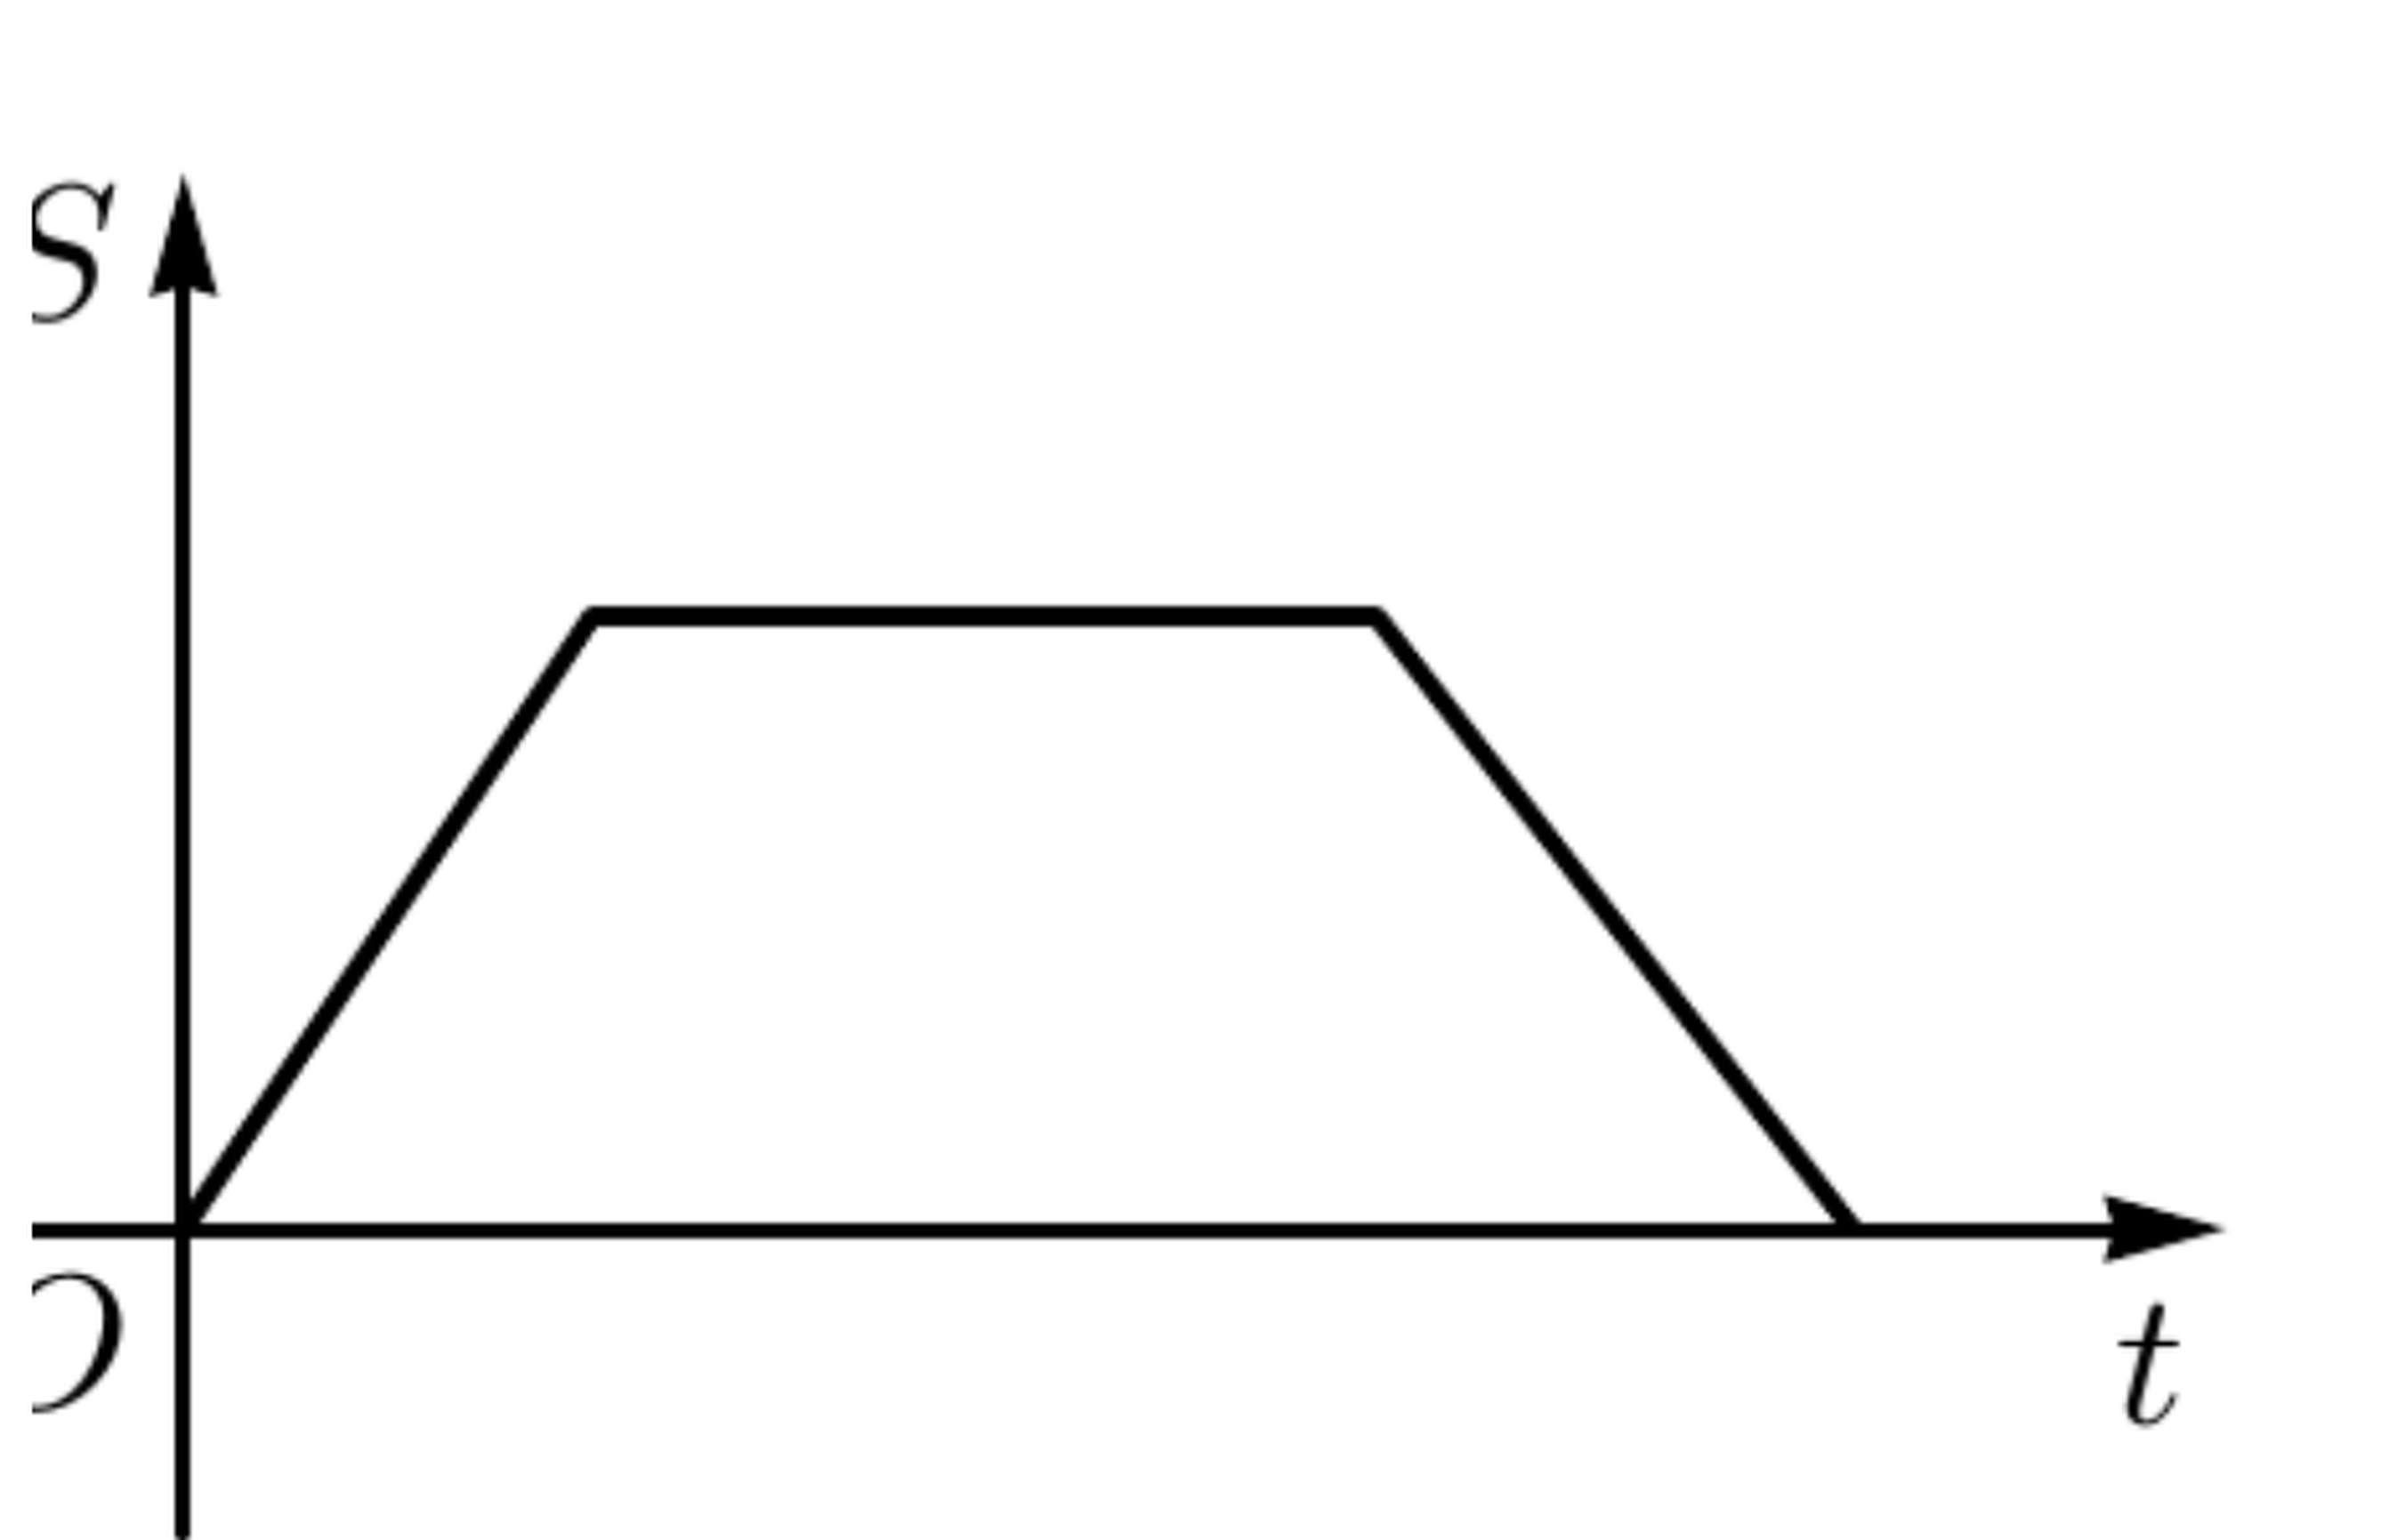
\includegraphics[width=0.34\textwidth]{figures/gao156_q14_st.png}
\end{center}

\keepwithprev
\begin{center}
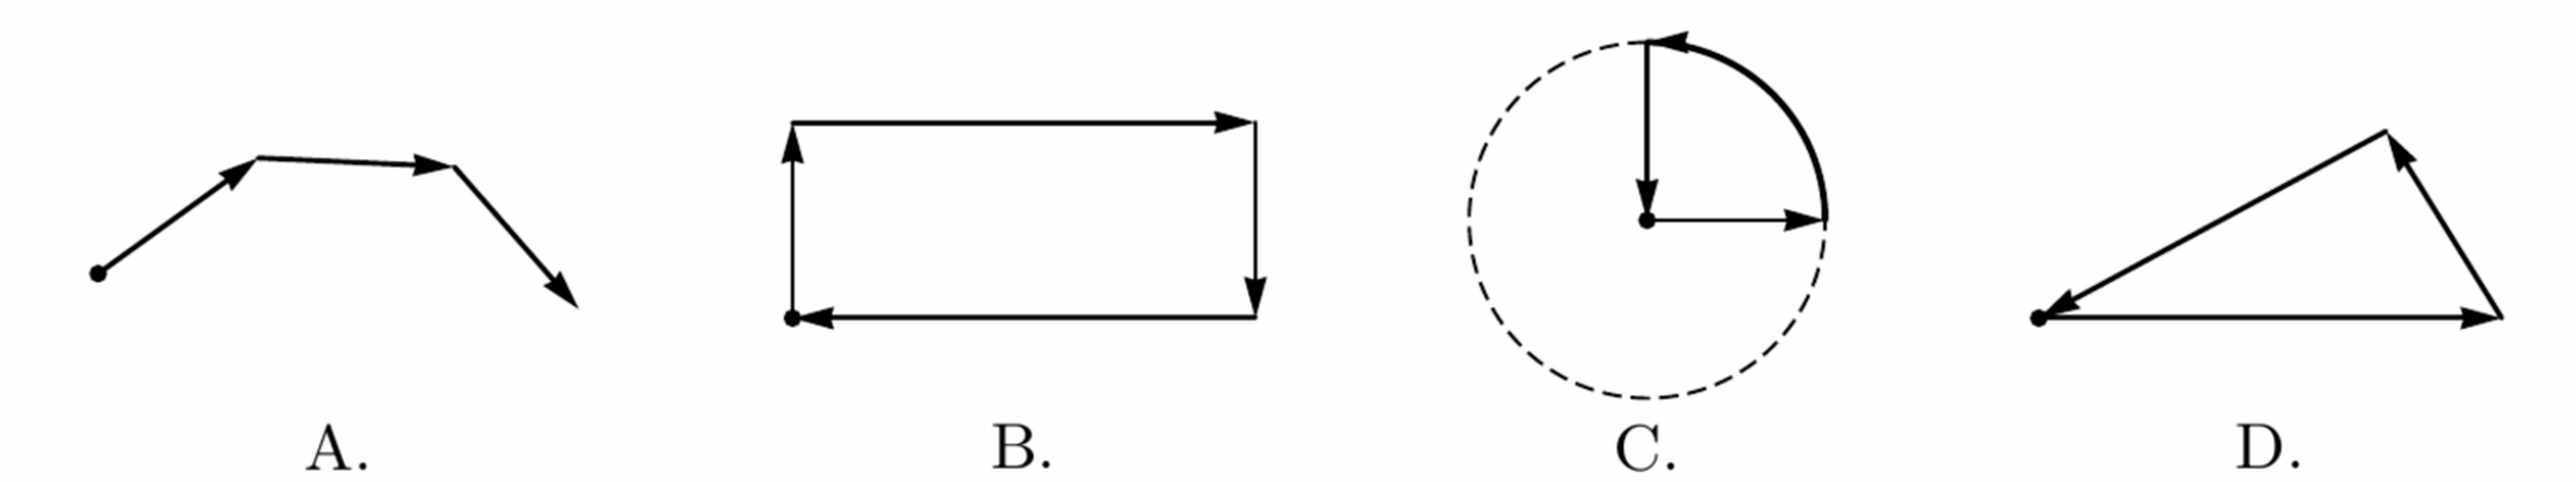
\includegraphics[width=0.86\textwidth]{figures/gao156_q14_opts.png}
\end{center}

\ifanswer
\solbegin
\step{由王老师锻炼时所走的离家距离（$S$）与行走时间（$t$）之间的函数关系图，}
\step{得在中间一段时间里，他到家的距离为定值，}
\step{故他所走的路程是一段以家为圆心的圆弧，故选 $C$.}
\solend
\fi

% === Q15 === 解析内曲线交点图（仅答案版出）；解析 4 行，故选 B
\item 已知 $a+2^a=b+\log_2 b=c+\log_3 c=k$，若 $k<1$，则\mbox{（\quad）}

\keepwithprev
A. $c<a<b$\qquad B. $a<c<b$\qquad C. $b<a<c$\qquad D. $a<b<c$

\ifanswer
\solbegin
\step{因为 $a+2^a=b+\log_2 b=c+\log_3 c=k$，}
\step{所以 $2^a=-a+k$，$\log_2 b=-b+k$，$\log_3 c=-c+k$，其中 $k<1$；}
\step{分别作出 $y=2^x$，$y=\log_2 x$，$y=\log_3 x$ 和 $y=-x+k$ 的图象，}

\begin{center}
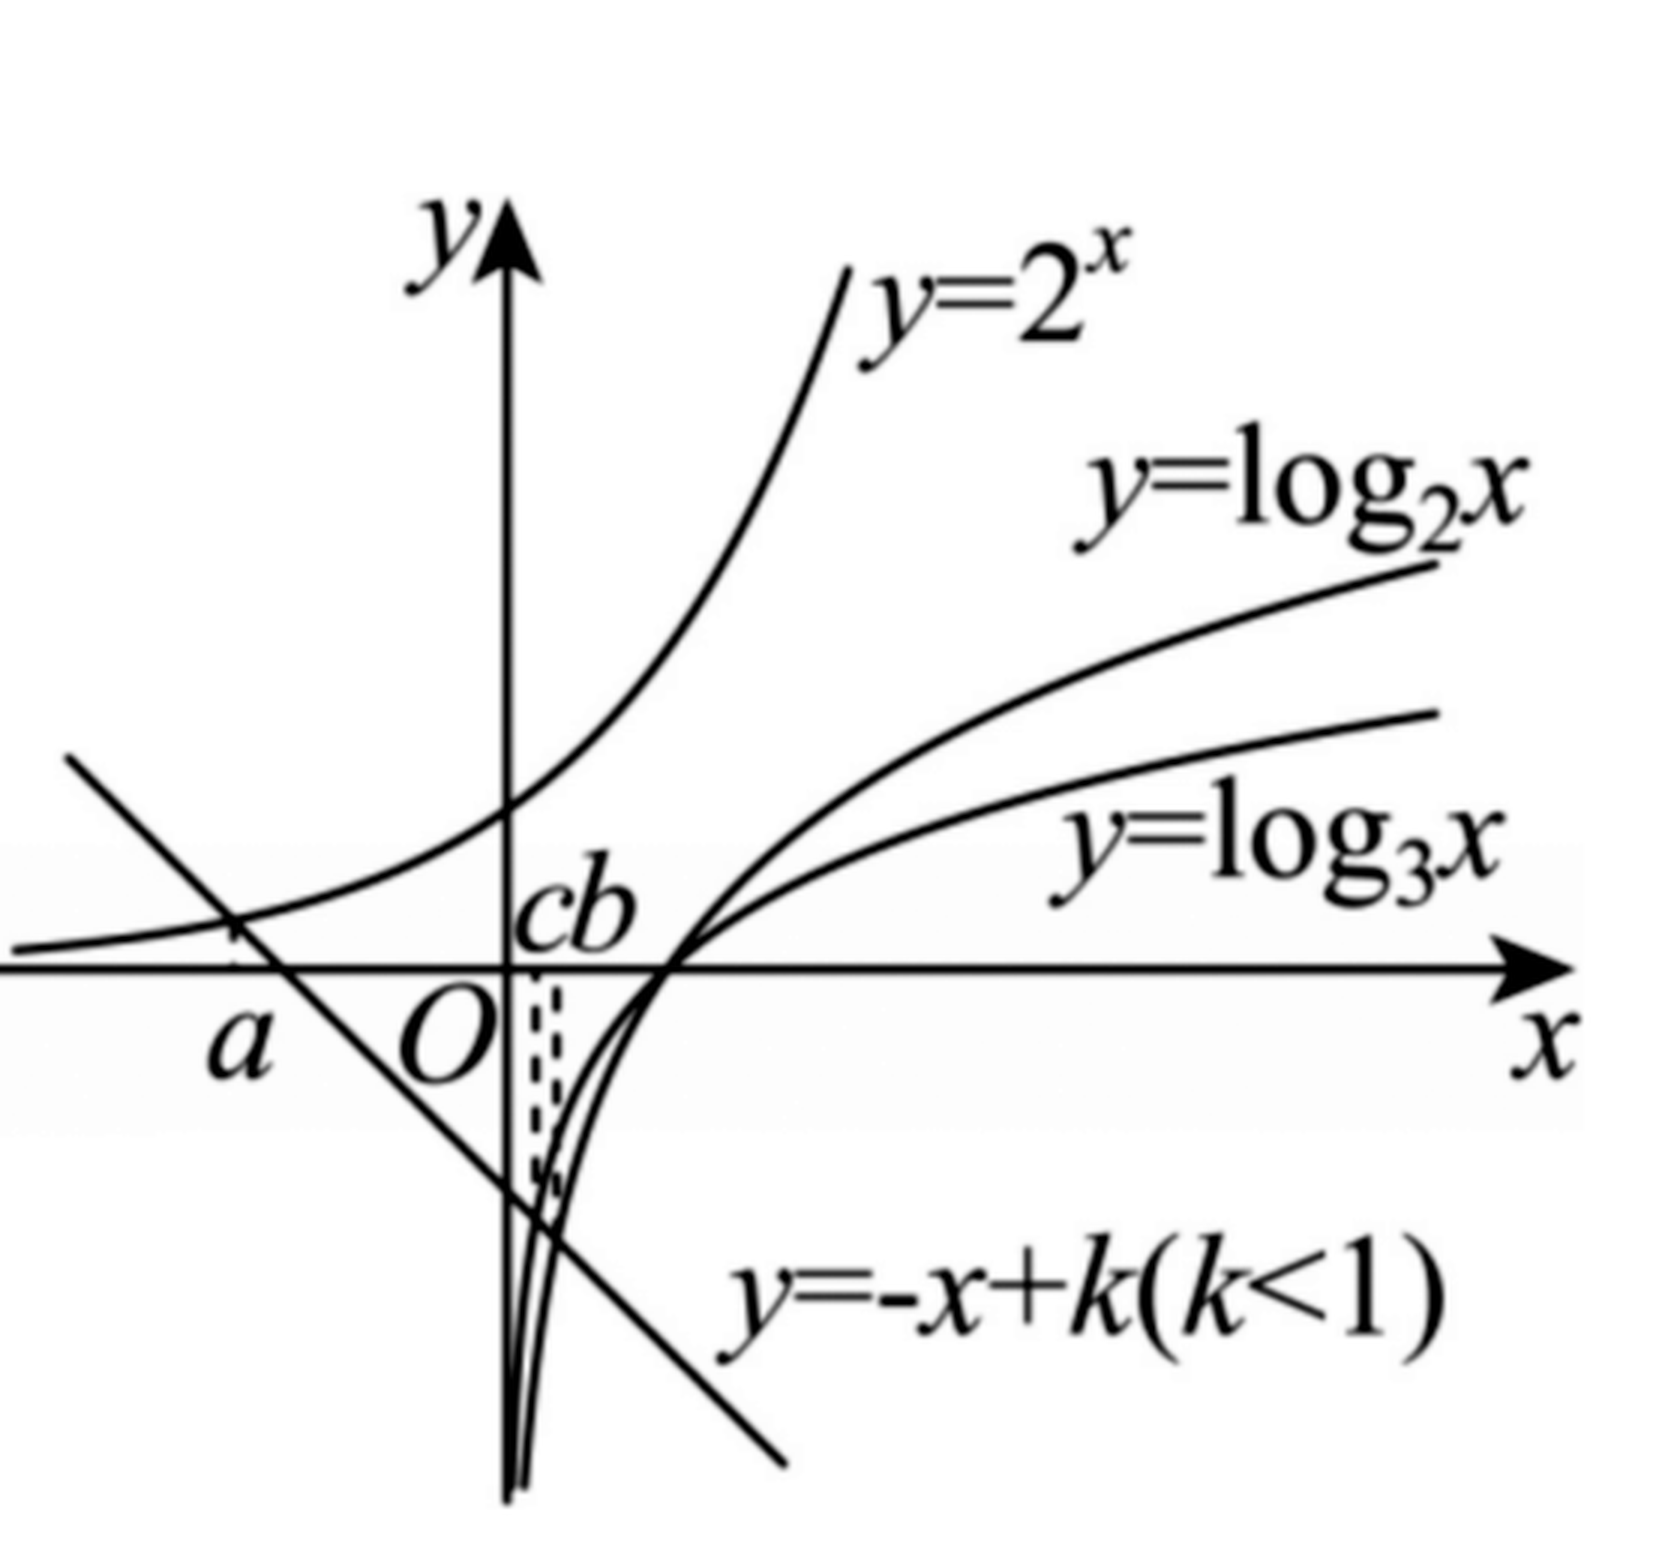
\includegraphics[width=0.52\textwidth]{figures/gao156_q15_curves.png}
\end{center}

\step{如图所示，由图象得 $a<c<b$. 故选 $B$.}
\solend
\fi

% === Q16 === ①② 文本圈数字、"一阶/二阶不动点""稳定点"自定义名词；解析 5 行，故选 A
\item 对定义域为 $I$ 的函数 $y=f(x)$，若存在 $x_0\in I$ 使得 $f(x_0)=x_0$，则称 $x_0$ 是函数 $f(x)$ 的
一阶不动点，简称不动点；若存在 $x_0\in I$ 使得 $f(f(x_0))=x_0$，则称 $x_0$ 是函数 $f(x)$ 的二阶
不动点，简称稳定点. 现有如下两个命题：①存在函数非 $y=x$ 且有无穷多个不动点；②
存在函数有无穷多个稳定点，且这些稳定点不都是不动点. 则\mbox{（\quad）}

\keepwithprev
A. ①成立，②成立\qquad\qquad B. ①成立，②不成立

C. ①不成立，②成立\qquad\qquad D. ①不成立，②不成立

\ifanswer
\solbegin
\step{①取定义在全体实数上的 $f(x)=\lvert x\rvert$，其不动点为一切非负实数，有无穷多个，}
\step{且 $f(-1)=1\ne-1$，①成立.}
\step{②取定义在全体实数上的 $g(x)=-x$，则 $g(g(x))=-(-x)=x$，}
\step{全体实数都是稳定点，而不动点只有 0，②成立.}
\step{故选 $A$.}
\solend
\fi

\end{enumerate}

\bigsec{三、解答题}

\begin{enumerate}
\setcounter{enumi}{16}

% === Q17 === $A\cap B$、$B\cap C$、\varnothing、\mid；解析 6 行
\item 设集合 $A=\{x\mid-1\leqslant x\leqslant2\}$，$B=\{x\mid2m<x<1\}$，$C=\{x\mid x<-1$ 或 $x>2\}$.

(1) 若 $A\cap B=B$，求实数 $m$ 的取值范围；

(2) 若 $B\cap C$ 中只有一个整数，求实数 $m$ 的取值范围.

\ifanswer
\solbegin
\step{(1) 当 $m\geqslant\dfrac12$ 时，$B=\varnothing$，满足 $A\cap B=B$.}
\step{当 $m<\dfrac12$ 时，$A\cap B=B$ 等价于 $2m\geqslant-1$，得 $-\dfrac12\leqslant m<\dfrac12$.}
\step{因此 $m$ 的取值范围为 $\left[-\dfrac12,+\infty\right)$.}
\step{(2) $B\cap C=\{x\mid2m<x<-1\}$，其中只有一个整数时，该整数必为 $-2$.}
\step{包含 $-2$ 且不包含 $-3$，等价于 $-3\leqslant2m<-2$，}
\step{因此 $m$ 的取值范围为 $\left[-\dfrac32,-1\right)$.}
\solend
\fi

% === Q18 === 幂函数 $x^{-\frac13}$、$m\in\R$；解析 12 行，跨 05—06 页
\item 已知幂函数 $f(x)=(3m^2-2m)x^m$（$m\in\R$）在定义域上不单调.

(1) 求函数 $f(x)$ 的解析式；

(2) 若 $f(a+1)<f(-2a+3)$，求实数 $a$ 的取值范围.

\ifanswer
\solbegin
\step{(1) 由幂函数的定义，$3m^2-2m=1$，即 $(3m+1)(m-1)=0$，得 $m=1$ 或 $m=-\dfrac13$.}
\step{当 $m=1$ 时，$f(x)=x$ 在定义域上单调递增，不合题意.}
\step{当 $m=-\dfrac13$ 时，$f(-1)=-1<f(1)=1$，而 $f(1)=1>f(8)=\dfrac12$，}
\step{故 $f(x)$ 在定义域上不单调.}
\step{因此 $f(x)=x^{-\frac13}$，定义域为 $(-\infty,0)\cup(0,+\infty)$.}
\step{(2) 有意义的条件为 $a\ne-1$ 且 $a\ne\dfrac32$.}
\step{当 $a<-1$ 时，$a+1<0<-2a+3$，有 $f(a+1)<0<f(-2a+3)$，}
\step{不等式成立.}
\step{当 $-1<a<\dfrac32$ 时，利用 $f(x)$ 在 $(0,+\infty)$ 上单调递减，}
\step{原不等式等价于 $a+1>-2a+3$，得 $\dfrac23<a<\dfrac32$.}
\step{当 $a>\dfrac32$ 时，$f(a+1)>0>f(-2a+3)$，不等式不成立.}
\step{所以 $a\in(-\infty,-1)\cup\left(\dfrac23,\dfrac32\right)$.}
\solend
\fi

% === Q19 === 两套解法（法一红字 \stepm，法二无标签）；\Delta 与 \subseteq；解析 21 行，跨 06—08 页
\item 已知 $a,c\in\R$，函数 $f(x)=\dfrac{x^2+(3a+1)x+c}{x+a}$.

(1) 若 $a=0$，求函数的定义域，并判断是否存在 $c$ 使得 $y=f(x)$ 图像关于原点对称，说明理由；

(2) 若函数过点 $(1,3)$，且函数 $y=f(x)$ 与 $x$ 轴负半轴有两个不同交点，求此时 $c$ 的值和 $a$ 的取值范围.

\ifanswer
\solbegin
\step{(1) 当 $a=0$ 时，$f(x)=\dfrac{x^2+(3a+1)x+c}{x+a}=\dfrac{x^2+x+c}{x}=x+\dfrac cx+1$，}
\step{故定义域为 $(-\infty,0)\cup(0,+\infty)$；}
\step{若存在实数 $c$，使得函数 $f(x)$ 为奇函数，则必有 $f(x)+f(-x)=0$，}
\step{而 $x+\dfrac cx+1+(-x)+\dfrac c{-x}+1=2\ne0$，}
\step{所以不存在实数 $c$，使得函数 $f(x)$ 为奇函数；}
\step{(2) 函数 $f(x)$ 的图像过点 $(1,3)$，则 $f(1)=\dfrac{1+(3a+1)+c}{1+a}=\dfrac{3a+c+2}{a+1}=3$，}
\step{解得 $c=1$，所以 $f(x)=\dfrac{x^2+(3a+1)x+1}{x+a}$，}
\stepm{法一：}{令 $f(x)=0$，则 $x^2+(3a+1)x+1=0$，此时方程有两不等负根，}
\step{则有 $\begin{cases}\Delta=(3a+1)^2-4>0\\-(3a+1)<0\end{cases}\Rightarrow\begin{cases}a>\dfrac13\text{ 或 }a<-1\\a>-\dfrac13\end{cases}\Rightarrow a>\dfrac13$，}
\step{注意到分母 $x+a\ne0$，则 $x\ne-a$，}
\step{若 $x=-a$ 也是方程 $x^2+(3a+1)x+1=0$ 的解，}
\step{代入方程 $(-a)^2+(3a+1)(-a)+1=0\Rightarrow2a^2+a-1=(a+1)(2a-1)=0$，}
\step{解得 $a=-1$ 或 $a=\dfrac12$，从而 $a\ne\dfrac12$，}
\step{综上，实数 $a$ 的取值范围为 $\left(\dfrac13,\dfrac12\right)\cup\left(\dfrac12,+\infty\right)$.}
\step{令 $g(x)=x^2+(3a+1)x+1$，与 $x$ 轴负半轴有两个交点，}
\step{则 $\begin{cases}-(3a+1)<0\\\Delta=(3a+1)^2-4>0\end{cases}\Rightarrow a>\dfrac13$.}
\step{注意到分母 $x+a\ne0$，则 $x\ne-a$，}
\step{若 $x=-a$ 也是方程 $x^2+(3a+1)x+1=0$ 的解，}
\step{代入方程 $(-a)^2+(3a+1)(-a)+1=0\Rightarrow2a^2+a-1=(a+1)(2a-1)=0$，}
\step{解得 $a=-1$ 或 $a=\dfrac12$，从而 $a\ne\dfrac12$，}
\step{综上，实数 $a$ 的取值范围为 $\left(\dfrac13,\dfrac12\right)\cup\left(\dfrac12,+\infty\right)$.}
\solend
\fi

% === Q20 === $Q$ 常数段 80000 照录；cases 与基本不等式；解析 10 行，跨 08—09 页
\item 某工厂生产某种零件的固定成本为 20000 元，每生产一个零件要增加投入 100 元，已知
总收入 $Q$（单位：元）关于产量 $x$（单位：个）满足函数：$Q=\begin{cases}400x-\dfrac12x^2,&0\leqslant x\leqslant400\\80000,&x>400\end{cases}$.

(1) 将利润 $P$（单位：元）表示为产量 $x$ 的函数；（总收入$=$总成本$+$利润）

(2) 当产量为何值时，零件的单位利润最大？最大单位利润是多少元？（单位利润$=$利润$\div$产量）

\ifanswer
\solbegin
\step{(1) 当 $0\leqslant x\leqslant400$ 时，}
\step{$P(x)=400x-\dfrac12x^2-20000-100x=-\dfrac12x^2+300x-20000$，}
\step{当 $x>400$ 时，$P(x)=80000-100x-20000=60000-100x$，}
\step{故 $P(x)=\begin{cases}-\dfrac12x^2+300x-20000,&0\leqslant x\leqslant400\\60000-100x,&x>400\end{cases}$.}
\step{(2) 设零件的单位利润为 $g(x)$，则 $g(x)=\begin{cases}-\dfrac12x-\dfrac{20000}{x}+300,&0\leqslant x\leqslant400\\\dfrac{60000}{x}-100,&x>400\end{cases}$，}
\step{当 $0\leqslant x\leqslant400$ 时，}
\step{$g(x)=300-\left(\dfrac12x+\dfrac{20000}{x}\right)\leqslant300-2\sqrt{\dfrac x2\cdot\dfrac{20000}{x}}=100$，}
\step{当且仅当 $\dfrac x2=\dfrac{20000}{x}$，即 $x=200$ 时取等号，}
\step{当 $x>400$ 时，$g(x)=\dfrac{60000}{x}-100$，此时无最值，}
\step{故当产量为 200 个，零件的单位利润最大，最大单位利润是 100 元.}
\solend
\fi

% === Q21 === 上升集定义、$D(x_0)=\{d\in\R\mid\cdots\}$、①②③ 文本圈数字、
%            \subseteq 带下划线、$-2^{-x}$；解析 19 行，跨 09—10 页
\item 已知函数 $y=f(x)$ 的定义域为 $\R$. 对任意 $x_0\in\R$，定义集合
$D(x_0)=\{d\in\R\mid f(x_0+d)>f(x_0)\}$，则称 $D(x_0)$ 为函数 $y=f(x)$ 在 $x_0$ 处的上升集.

(1) 若 $f(x)=1-x$，求 $D(-1)$；

(2) 若 $f(x)=\begin{cases}2^x,&x<0\\0,&x=0\\-2^{-x},&x>0\end{cases}$，求 $D(x)$；

(3) 设 $y=f(x)$ 满足：①当 $x<0$ 时，$f(x)=2^x$；②若 $f(x_1)\leqslant f(x_2)$，则
$D(x_2)\subseteq D(x_1)$；③当 $0<x<1$ 时，$f(x)<f(0)$. 证明：$f(0)\geqslant1$.

\ifanswer
\solbegin
\step{(1) $f(-1+d)>f(-1)\Leftrightarrow2-d>2\Leftrightarrow d<0$，所以 $D(-1)=(-\infty,0)$.}
\step{(2) 函数在 $(-\infty,0)$、$(0,+\infty)$ 上分别严格递增，}
\step{且这两个区间上的函数值分别为正、负，$f(0)=0$.}
\step{当 $x<0$ 时，$f(x+d)>f(x)\Leftrightarrow x<x+d<0\Leftrightarrow0<d<-x$，}
\step{当 $x=0$ 时，$f(d)>f(0)\Leftrightarrow d<0$，}
\step{当 $x>0$ 时，$f(x+d)>f(x)\Leftrightarrow x+d\leqslant0$ 或 $x+d>x$}
\step{$\Leftrightarrow d\leqslant-x$ 或 $d>0$，}
\step{因此 $D(x)=\begin{cases}(0,-x),&x<0\\(-\infty,0),&x=0\\(-\infty,-x]\cup(0,+\infty),&x>0\end{cases}$.}
\step{(3) 任取 $a\in(-1,0)$，}
\step{令 $d=-\dfrac a2$，则 $0<d<1$，且 $f(a+d)=2^{\frac a2}>2^a=f(a)$，}
\step{所以 $d\in D(a)$；}
\step{由③，$f(d)<f(0)$，所以 $d\notin D(0)$.}
\step{若 $f(0)\leqslant f(a)$，由②得 $D(a)\subseteq D(0)$，与上述结论矛盾.}
\step{因此，对任意 $a\in(-1,0)$，都有 $f(0)>2^a$.}
\step{特别地 $f(0)>2^{-\frac12}>0$.}
\step{若 $f(0)<1$，取 $a=\dfrac12\log_2 f(0)$，则 $-\dfrac14<a<0$，且}
\step{$2^a=\sqrt{f(0)}>f(0)$，}
\step{与 $f(0)>2^a$ 矛盾.}
\step{所以 $f(0)\geqslant1$.}
\solend
\fi

\end{enumerate}

\end{document}
"
%
% ① 原始材料：微信公众号"魔都数学加油站"文章，连载"27学年高一156"，原文标题
% "27学年高一156——2026-2027年上海市大同中学高一上期中"；
% 原文链接：https://mp.weixin.qq.com/s/xLtS5tyjCPJIWCIBohwGvw 。
% 正文为 10 张 PNG 页（01/02/03/04/05/06/07/08/09/10 各页分辨率混排
% 2560×3620 与 4762×6735，逐页按各自分辨率裁图核对）。
% 体例：讲评版——填空 3—12（10 题）、选择 13—16（4 题）、解答 17—21（5 题），
% 共 19 题，自第 3 题起编（1、2 未印在本篇）；Q3 只印【答案】、其余 18 题
% 逐题印【解析】（逐题核实，见 ②）。题目、答案、解析均据原图转录；卷面粉红色
% 水印"魔都数学加油站"及公众号页脚未录入。
%
% 卷首标题：原卷印作"2026-2027 年大同中学高一上期中"，年份区间按全稿惯例排 en dash；
% 原卷卷面未印副标题，本稿按同期中卷知识模块口径补出"集合与常用逻辑用语、不等式、函数"。
%
% ② 与原卷的排版差异：
%   ① 原文从第 3 题起，本稿保留原题号；共 19 题三节，解答题 5 题到 21；
%   ② 混合体例：第 3 题只印【答案】、无【解析】，按 高一140 第 5 题／高一145
%      第 3 题／高一151 第 7 题成例另提 \ans{}、不补造解析；其余 18 题印
%      【解析】、用 \solbegin…\solend；四道选择题答案在解析末句"故选 C／C／B／A"
%      （逐个放大复核）、括号 \mbox{（\quad）} 留空、不另提 \ans{}；答案版
%      【答案】/【解析】标记数 = 19 = 全卷题数（1 个 \ans ＋ 18 个 \solbegin）；
%   ③ 原卷卷面未印副标题，本稿按知识模块口径补出；
%   ④ 原卷填空横线按全稿惯例排 \blankline[4.4em]；选择题括号排 \mbox{（\quad）}、
%      选项段前按惯例各加 \keepwithprev；解答题不留作答区、不加 \anspace
%      （原卷为讲评版，109—113 起全稿不用 \anspace）；
%   ⑤ 数集：Q3"$x\in\R$"、Q18"$m\in\R$"、Q19"$a,c\in\R$"、Q21"定义域为 \R"
%      "任意 $x_0\in\R$""$d\in\R$"原卷印正体粗体 R，按全稿惯例归一 \R；
%      绝对值排 \lvert…\rvert（Q11 $\lvert2^x-1\rvert$、Q16 $\lvert x\rvert$），
%      集合描述竖线排 \mid（Q17 $A=\{x\mid\cdots\}$、Q21 $D(x_0)=\{d\in\R\mid\cdots\}$），
%      空集 \varnothing（Q17"$B=\varnothing$"），不等号按全稿惯例排 \leqslant／\geqslant；
%   ⑥ 子集符号逐处照录不统一：Q21 (3) 题干"$D(x_2)\subseteq D(x_1)$"与解析
%      "$D(a)\subseteq D(0)$"均印带下划线 ⊆，照录 \subseteq；本卷无单线 ⊂ 用例；
%   ⑦ 判别式：Q19 两套解法"$\Delta=(3a+1)^2-4>0$"印等腰偏高 \Delta，照录 \Delta；
%      本卷无扁三角 \triangle 用例；
%   ⑧ 红字照录为黑体：Q19 (2) 解析第一套解法行首"法一："原卷排**红色加粗**，
%      按 高一53 成例排 \stepm{法一：}{…}（加粗着色、不改黑色基调），全库无红字
%      排字先例、本稿不引入红色定义，文件头注明；第二套解法原卷直接以
%      "令 $g(x)=x^2+(3a+1)x+1$，与 $x$ 轴负半轴有两个交点，"另起，
%      **未印"法二："标签**（逐页像素级复核：07 页仅 1437—1475 一处红字，
%      08 页无红字），照录为普通 \step、不补造标签；
%   ⑨ 文本模式圈数字逐处照录：Q12 解析 ①② 两情形、Q16 两则命题与四个选项及
%      解析的 ①②、Q21 (3) 三条件 ①②③ 与解析"由③""由②"，均为印刷圈数字
%      （非 \textcircled、非数学模式），计入圈数字实测；
%   ⑩ 自定义名词照录：Q16"一阶不动点，简称不动点""二阶不动点，简称稳定点"、
%      Q21"上升集"；Q16 题干"存在函数非 $y=x$ 且有无穷多个不动点"照录；
%   ⑪ 中文弯引号照录：Q3""存在 $x\in\R$，$x^3-1\leqslant0$" 否定形式为"、
%      Q13"使"$\dfrac{x+1}{1-x}\geqslant0$"成立的必要不充分条件是"；
%      注释里一律 ASCII 引号；数学式内 CJK 用 \text{}（Q19 cases 内"或"）；
%   ⑫ 半角逗号在数学组之间是全稿惯例、非笔误，逐处照录（$a,c$、$x,y$、$a,b$
%      之类）；行末西文句点 ASCII `.`；行中全角逗号／顿号照录；
%   ⑬ 复杂式照录别简化：Q6 $\left(\dfrac{1}{\sqrt a}\right)^{\frac27}\cdot\sqrt[7]{a^3}$
%      与解析 $a^{\frac{12}{7}-\frac17+\frac37}$、Q8 $2\sqrt4+5=9$（$\sqrt4$ 未化简）、
%      Q9 $\left(\sqrt x+\dfrac{1}{\sqrt x}\right)^3$、Q12 $\dfrac{4a-(2-a)^2}{4a}$、
%      Q18 $f(8)=\dfrac12$、Q19 $2a^2+a-1=(a+1)(2a-1)=0$、Q20 $Q$ 的常数段
%      $80000$（不是 $80000-100x$）与 $2\sqrt{\dfrac x2\cdot\dfrac{20000}{x}}$、
%      Q21 $f(a+d)=2^{\frac a2}>2^a=f(a)$ 与 $2^a=\sqrt{f(0)}>f(0)$ 等；
%      \left…\right 不得拆到不同 $…$ 组（Q5 $\left(0,\dfrac12\right)$、
%      Q12 $\left[0,4+2\sqrt3\right)$、Q17 $\left[-\dfrac12,+\infty\right)$、
%      Q19 $\left(\dfrac13,\dfrac12\right)\cup\left(\dfrac12,+\infty\right)$、
%      Q20 $\left(\dfrac12x+\dfrac{20000}{x}\right)$ 等）；cases 块整体算一个印刷行；
%   ⑭ 一条 \step = 原卷解析的一个印刷行；别并折行、别拆行。跨页续印按题合并
%      （Q6 的 01 页上下题干重复印、Q8 的 01—02 页、Q12 的 02—03 页、
%      Q15 的 04 页上下、Q16 的 04—05 页、Q17 的 05 页上下、Q18 的 05—06 页、
%      Q19 的 06—08 页、Q20 的 08—09 页、Q21 的 09—10 页）；
%      跨半页重叠行（Q12 的"②若 …"、Q18 的"原不等式等价于 …"、
%      Q20 的"【解析】(1) 当 $0\leqslant x\leqslant400$ 时，"、Q21 的
%      "【解析】(1) $f(-1+d)>f(-1)\cdots$"与"与 $f(0)>2^a$ 矛盾."）
%      只算一个印刷行；
%   ⑮ 配图：全卷 3 组（逐页通读 10 页确认）——
%      · Q14 题干 S-t 梯形图（03 页右下，离家距离 S 对行走时间 t），题目配图、
%        三版都出，裁 figures/gao156_q14_st.png；
%      · Q14 四幅路线选项（04 页上部，A/B/C/D 四幅横排、C 为以家为圆心的圆弧），
%        题目配图、三版都出，合并成一张，裁 figures/gao156_q14_opts.png；
%      · Q15 解析内曲线交点图（04 页右下，$y=2^x$、$y=\log_2x$、$y=\log_3x$
%        与 $y=-x+k$），仅答案版出，裁 figures/gao156_q15_curves.png；
%      3 图均取自原卷截图，去粉色水印、去色、3×~4× LANCZOS 放大；
%      Q14 题干"题干＋两图"整块用 \needvspace 守卫推走（守卫放 \item 之前，
%      见 高一154 Q15／高一136 Q13 成例）；Q15 解析内图放 \ifanswer 内
%      \solbegin…\solend 的两 \step 之间（高一108 第 6 题／高一154 附加题 2 成例）；
%      其余各页逐页确认无其它题目配图、无解析配图、无表格；10 页下半仅水印、无正文。
%
% ③ 行数复核：一条 \step = 原卷解析的一个印刷行，cases 块作一个印刷行计。
%   逐题数（主会话逐页核对定稿）：Q3：0（只印【答案】、提 \ans{}，不计入 \step 账）；
%   Q4：1；Q5：1；Q6：1；Q7：1；Q8：3；Q9：2；Q10：2；Q11：5；Q12：12；
%   Q13：3；Q14：3；Q15：4；Q16：5；Q17：6；Q18：12；Q19：21；Q20：10；Q21：19。
%   合计 111 行（110 条 \step ＋ 1 条 \stepm），与原卷逐题印刷行相等。
%   全卷 19 题：Q3 一处 \ans{} ＋ 其余 18 题设 \solbegin…\solend，
%   答案版【答案】/【解析】标记数 = 19 = 全卷题数。
%
% ④ 页码分布（供回原图复核）：
%   卷首标题＋"一、填空题"＋Q3 题干＋【答案】、Q4 题干＋解析 1 行、
%   Q5 题干＋解析 1 行、Q6 题干首行在 01 页上半；
%   Q6 题干（重复印）＋解析 1 行、Q7 题干＋解析 1 行、Q8 题干＋解析前 2 行
%   在 01 页下半；Q8 解析末行、Q9 题干＋解析 2 行、Q10 题干＋解析 2 行、
%   Q11 题干首行在 02 页上半；Q11 题干（重复印）＋解析 5 行、
%   Q12 题干＋解析首行在 02 页下半；Q12 解析中 9 行在 03 页上半；
%   Q12 解析末 2 行＋"二、选择题"标题＋Q13 题干＋选项＋解析 3 行＋
%   Q14 题干首行在 03 页下半；Q14 题干续行＋四幅选项图＋解析 3 行＋
%   Q15 题干＋选项＋解析前 2 行＋Q16 题干在 04 页上半；
%   Q15 解析后 2 行＋曲线图＋Q16 选项＋解析前 2 行在 04 页下半；
%   Q16 解析后 3 行＋"三、解答题"标题＋Q17 题干＋两问＋解析 (1) 3 行
%   在 05 页上半；Q17 解析 (2) 3 行＋Q18 题干＋两问＋解析 (1) 首 2 行
%   在 05 页下半；Q18 解析 (1)(2) 中 8 行在 06 页上半；Q18 解析末 2 行＋
%   Q19 题干＋两问＋解析 (1) 首行在 06 页下半；Q19 解析 (1) 后 4 行＋
%   (2) 前 2 行＋法一 2 行在 07 页上半；法一后 5 行＋法二前 3 行在 07 页下半；
%   法二后 4 行＋Q20 题干＋两问＋解析 (1) 首行在 08 页上半；
%   Q20 解析 (1) 后 3 行＋(2) 前 5 行在 08 页下半；Q20 解析 (2) 末 2 行＋
%   Q21 题干＋三问＋解析 (1) 首行在 09 页上半；Q21 解析 (1)（重复印）＋
%   (2) 8 行＋(3) 首行在 09 页下半；Q21 (3) 解析中 8 行在 10 页上半；
%   Q21 (3) 末 2 行在 10 页下半。本稿按题连排，不丢行、不并折行；
%   全卷末题为第 21 题，无附加题节。
%
\documentclass[a4paper,11pt]{article}
\usepackage{common}

\begin{document}

\examtitlest[3]{2026--2027 年大同中学高一上期中}{集合与常用逻辑用语、不等式、函数}

\bigsec{一、填空题}

\begin{enumerate}
\setcounter{enumi}{2}

% === Q3 === 只印【答案】、无【解析】；R 正体粗体 \R；中文弯引号照录
\item “存在 $x\in\R$，$x^3-1\leqslant0$” 否定形式为\blankline[4.4em].

\ifanswer
\ans{对任意 $x\in\R$，$x^3-1>0$}
\fi

% === Q4 === 解析 1 行
\item 若实数 $a>0$ 且 $a\ne1$，函数 $y=a^{x-3}+1$ 的图像恒过定点 $P$，则点 $P$ 的坐标为\blankline[4.4em].

\ifanswer
\solbegin
\step{当 $x=3$ 时，$y=a^0+1=2$，与 $a$ 无关，所以定点为 $P(3,2)$.}
\solend
\fi

% === Q5 === 解析 1 行
\item 函数 $y=\dfrac{1}{3^x+2}$ 的值域是\blankline[4.4em].

\ifanswer
\solbegin
\step{$3^x\in(0,+\infty)$，因此 $3^x+2\in(2,+\infty)$，值域为 $\left(0,\dfrac12\right)$.}
\solend
\fi

% === Q6 === 根式嵌套照录；解析 1 行；题干跨 01 页上下重复印
\item 已知 $a>0$，化简 $a^{\frac{12}{7}}\cdot\left(\dfrac{1}{\sqrt a}\right)^{\frac27}\cdot\sqrt[7]{a^3}=$\blankline[4.4em].

\ifanswer
\solbegin
\step{原式 $=a^{\frac{12}{7}}\cdot a^{-\frac17}\cdot a^{\frac37}=a^{\frac{12}{7}-\frac17+\frac37}=a^2$.}
\solend
\fi

% === Q7 === 换底公式；解析 1 行
\item 已知 $\log_5 3=a$，用 $a$ 的代数式表示 $\log_{15}125=$\blankline[4.4em].

\ifanswer
\solbegin
\step{$\log_{15}125=\dfrac{\log_5 125}{\log_5 15}=\dfrac{3}{1+\log_5 3}=\dfrac{3}{1+a}$.}
\solend
\fi

% === Q8 === 基本不等式，$\sqrt4$ 照录未化简；解析 3 行，跨 01—02 页
\item 已知 $x>0$，$y>0$，且 $4x+y=xy$，则 $x+y$ 的最小值为\blankline[4.4em].

\ifanswer
\solbegin
\step{由 $4x+y=xy$，得 $\dfrac4y+\dfrac1x=1$，}
\step{则 $x+y=(x+y)\left(\dfrac4y+\dfrac1x\right)=\dfrac{4x}{y}+\dfrac yx+1+4\geqslant2\sqrt4+5=9$，}
\step{当且仅当 $\dfrac{4x}{y}=\dfrac yx$，即 $x=3$，$y=6$ 时取等号，故最小值为 9.}
\solend
\fi

% === Q9 === 解析 2 行
\item 已知 $x^{-1}+x=7$（$x>0$），则 $x^{\frac32}+x^{-\frac32}$ 的值为\blankline[4.4em].

\ifanswer
\solbegin
\step{$x>0$，有 $\sqrt x+\dfrac{1}{\sqrt x}=\sqrt{x+\dfrac1x+2}=3$，}
\step{所以 $x^{\frac32}+x^{-\frac32}=\left(\sqrt x+\dfrac{1}{\sqrt x}\right)^3-3\left(\sqrt x+\dfrac{1}{\sqrt x}\right)=27-9=18$.}
\solend
\fi

% === Q10 === $x_{\min}$；解析 2 行
\item 已知不等式 $x>\dfrac{2a+1}{a-1}$ 对任意的 $x\in[1,2]$ 恒成立，则实数 $a$ 的取值范围是\blankline[4.4em].

\ifanswer
\solbegin
\step{不等式 $x>\dfrac{2a+1}{a-1}$ 对任意的 $x\in[1,2]$ 恒成立，得 $\dfrac{2a+1}{a-1}<x_{\min}=1$，}
\step{即有 $\dfrac{a+2}{a-1}<0$，解得 $-2<a<1$，则实数 $a$ 的取值范围是 $(-2,1)$.}
\solend
\fi

% === Q11 === 分段函数 cases 与绝对值 \lvert…\rvert；解析 5 行
\item 已知函数 $f(x)=\begin{cases}\lvert2^x-1\rvert-a,&x\leqslant2\\\dfrac{3}{x-1}-a,&x>2\end{cases}$，若函数 $y=f(x)$ 图像与 $x$ 轴有三个不同交点，则实数 $a$ 的取值范围是\blankline[4.4em].

\ifanswer
\solbegin
\step{令 $g(x)=f(x)+a$.}
\step{在 $(-\infty,0)$、$[0,2]$、$(2,+\infty)$ 上，$g(x)$ 均严格单调，}
\step{值域依次为 $(0,1)$、$[0,3]$、$(0,3)$.}
\step{每段至多有一个交点，因而恰有三个不同交点，}
\step{当且仅当 $a\in(0,1)\cap[0,3]\cap(0,3)=(0,1)$.}
\solend
\fi

% === Q12 === ①② 文本圈数字、对称轴与最小值式照录；解析 12 行，跨 02—03 页
\item 已知函数 $f(x)=ax^2-(2-a)x+1$，$g(x)=x$，若对于任意实数 $x$，$f(x)$ 与 $g(x)$ 至少有一个为正数，则实数 $a$ 的取值范围是\blankline[4.4em].

\ifanswer
\solbegin
\step{当 $x>0$ 时，$g(x)>0$；当 $x<0$ 时，$g(x)<0$；}
\step{当 $x=0$ 时，$f(0)=1>0$；}
\step{因为对于任意实数 $x$，$f(x)$ 与 $g(x)$ 至少有一个为正数，}
\step{当 $x<0$ 时，因为 $g(x)<0$，所以 $f(x)=ax^2-(2-a)x+1>0$ 恒成立，}
\step{当 $a<0$ 时，显然不成立，}
\step{当 $a=0$ 时，$f(x)=-2x+1>0$，对 $x<0$ 时恒成立，满足题意，}
\step{当 $a>0$ 时，函数图象开口向上，对称轴 $x=\dfrac{2-a}{2a}$，}
\step{①若 $\dfrac{2-a}{2a}\geqslant0$，即 $0<a\leqslant2$ 时，函数 $f(x)$ 在 $(-\infty,0)$ 上严格减，$f(0)=1$，}
\step{故 $f(x)>0$ 对 $x<0$ 时恒成立，满足题意；}
\step{②若 $\dfrac{2-a}{2a}<0$，即 $a>2$ 时，$f(x)_{\min}=f\left(\dfrac{2-a}{2a}\right)=\dfrac{4a-(2-a)^2}{4a}>0$，}
\step{解得 $4-2\sqrt3<a<4+2\sqrt3$，所以 $2<a<4+2\sqrt3$.}
\step{综上，$0\leqslant a<4+2\sqrt3$，故实数 $a$ 的取值范围是 $\left[0,4+2\sqrt3\right)$.}
\solend
\fi

\end{enumerate}

\bigsec{二、选择题}

\begin{enumerate}
\setcounter{enumi}{12}

% === Q13 === 必要不充分条件；cases 块；解析 3 行，故选 C
\item 使 “$\dfrac{x+1}{1-x}\geqslant0$” 成立的必要不充分条件是\mbox{（\quad）}

\keepwithprev
A. $-1\leqslant x<1$\qquad B. $x\leqslant-1$ 或 $x>1$\qquad C. $-1\leqslant x\leqslant1$\qquad D. $x\leqslant-1$ 或 $x\geqslant0$

\ifanswer
\solbegin
\step{由不等式 $\dfrac{x+1}{1-x}\geqslant0$ 得 $\begin{cases}(x+1)(1-x)\geqslant0\\1-x\ne0\end{cases}$，解得 $-1\leqslant x<1$，}
\step{由题意结合选项，$-1\leqslant x<1\Rightarrow-1\leqslant x\leqslant1$ 成立，反之不成立，}
\step{所以 $-1\leqslant x\leqslant1$ 是 $\dfrac{x+1}{1-x}\geqslant0$ 成立的必要不充分条件. 故选 $C$.}
\solend
\fi

% === Q14 === 题干 S-t 图＋四幅路线选项（题目配图，三版都出）；守卫放 \item 之前；解析 3 行，故选 C
\needvspace{9cm}
\item 如图是王老师锻炼时所走的离家距离（$S$）与行走时间（$t$）之间的函数关系图，若
用黑点表示王老师家的位置，则王老师行走的路线可能是\mbox{（\quad）}

\begin{center}
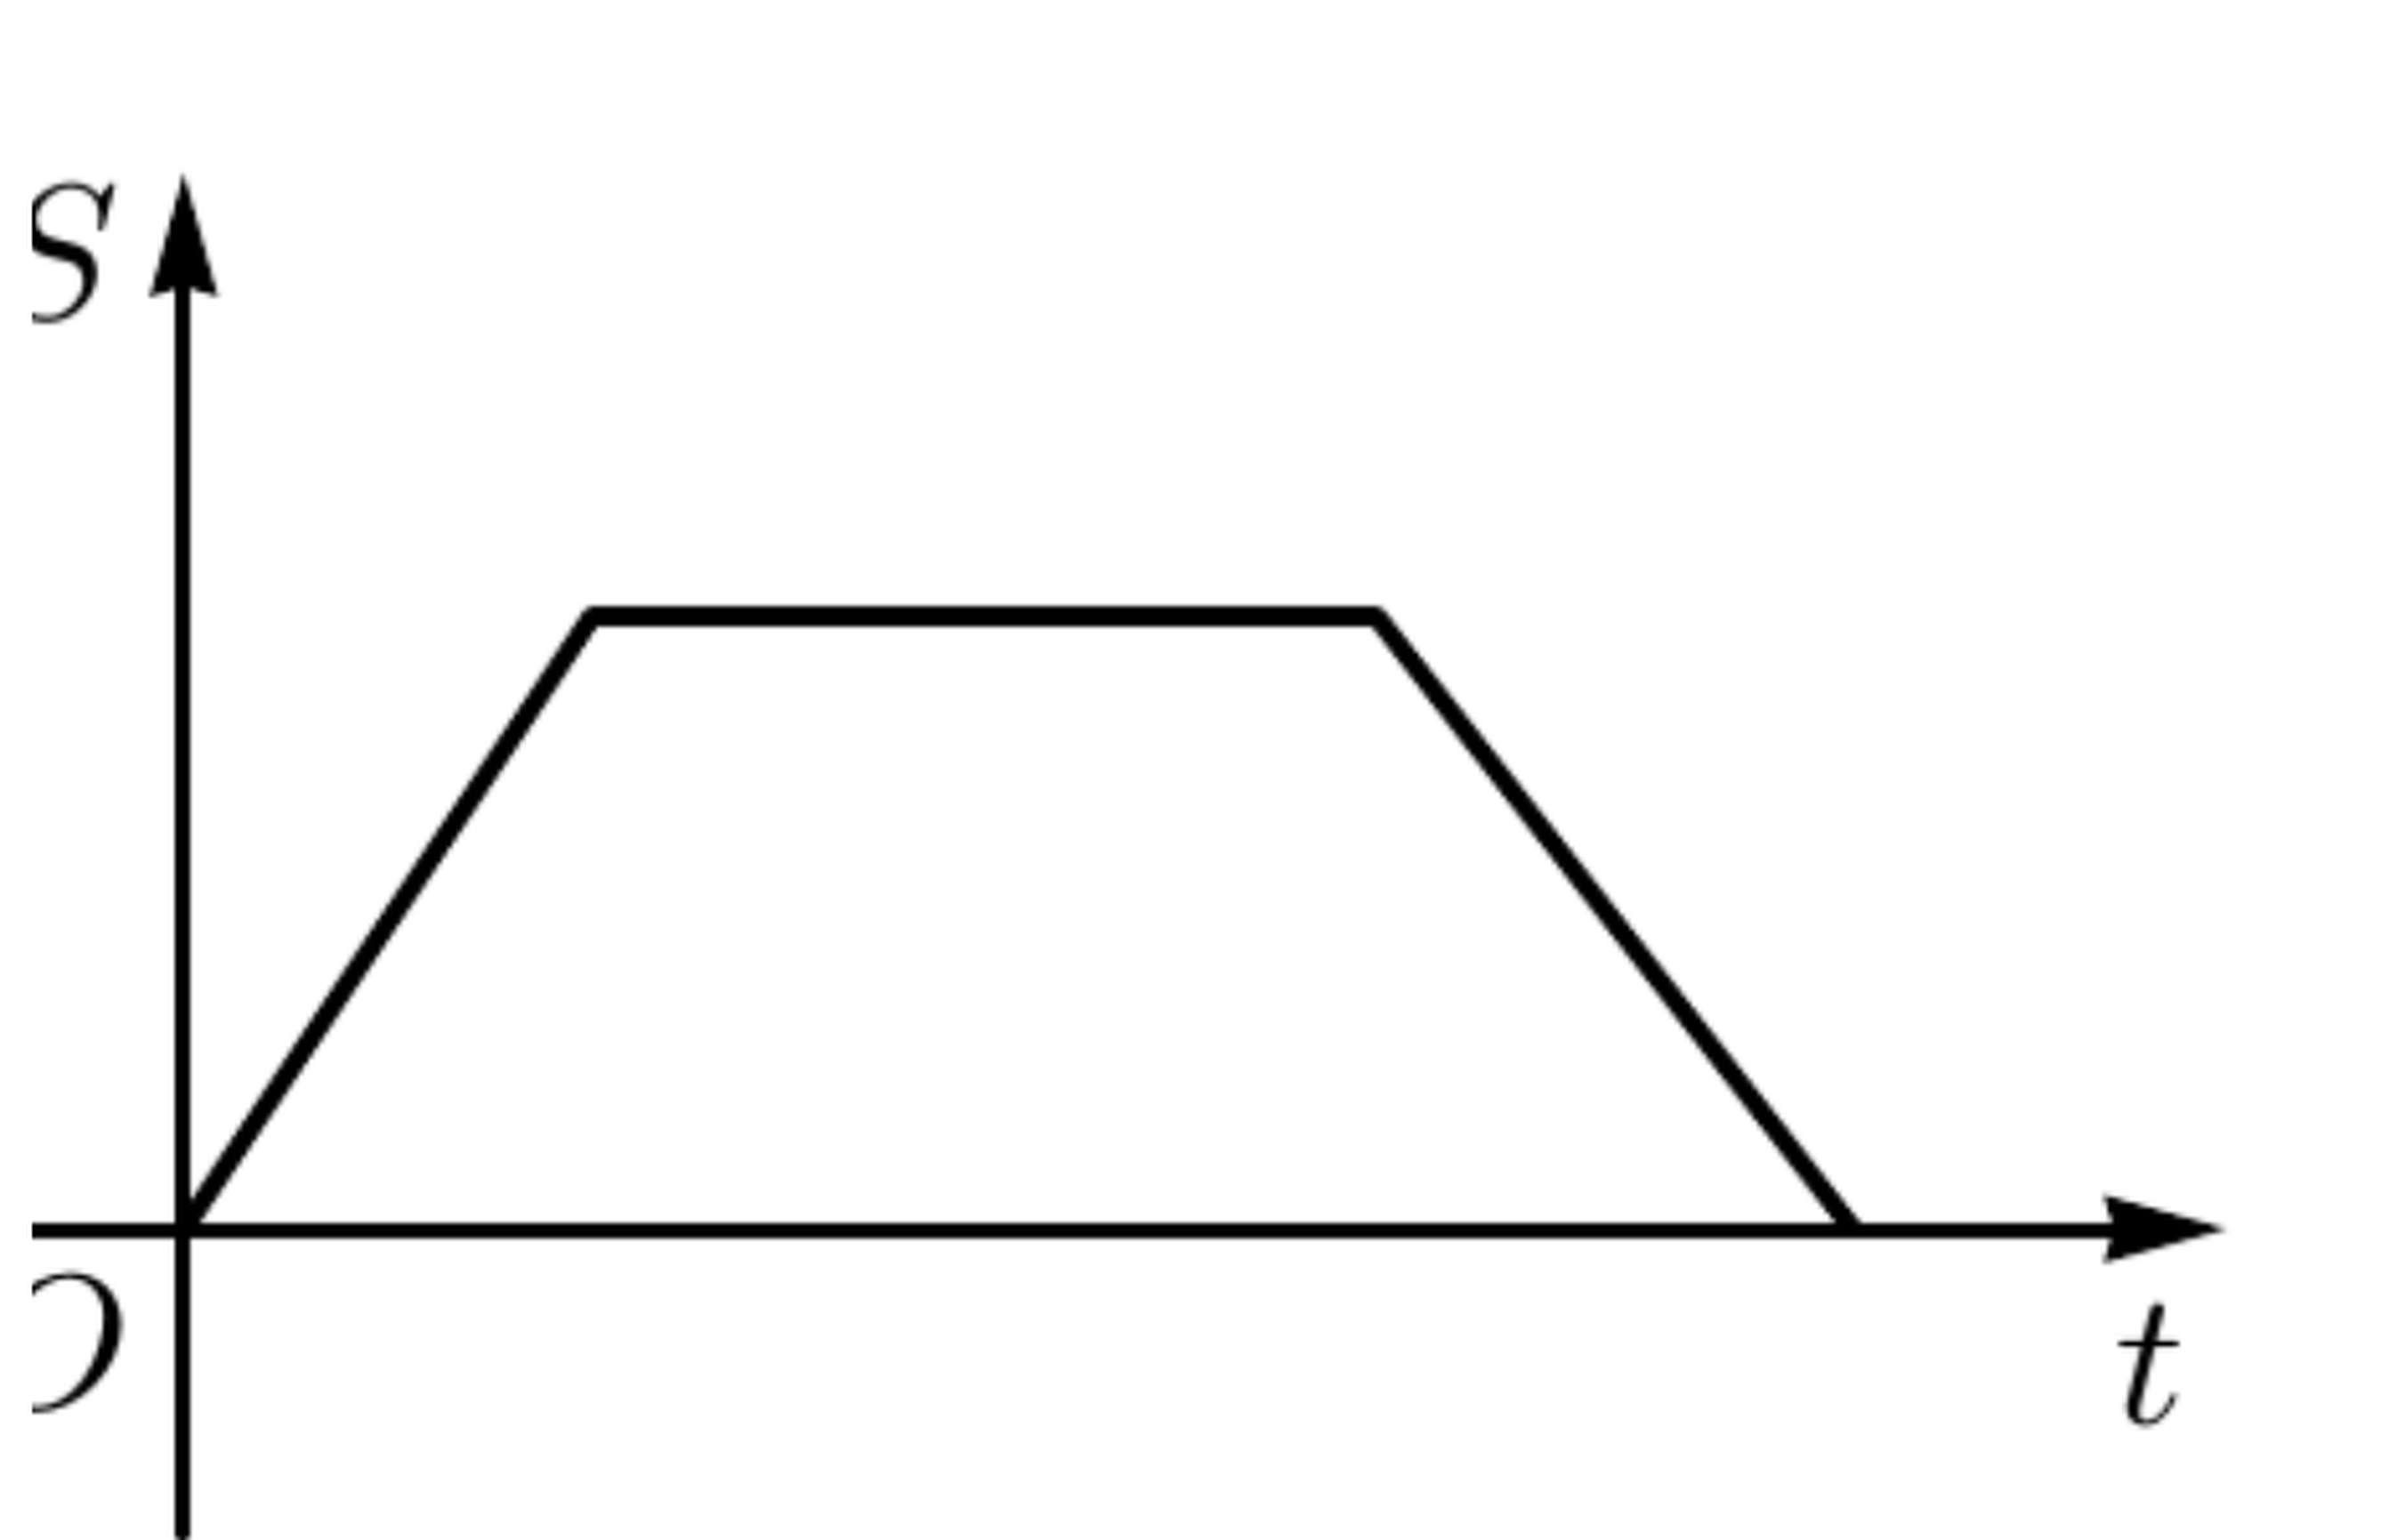
\includegraphics[width=0.34\textwidth]{figures/gao156_q14_st.png}
\end{center}

\keepwithprev
\begin{center}
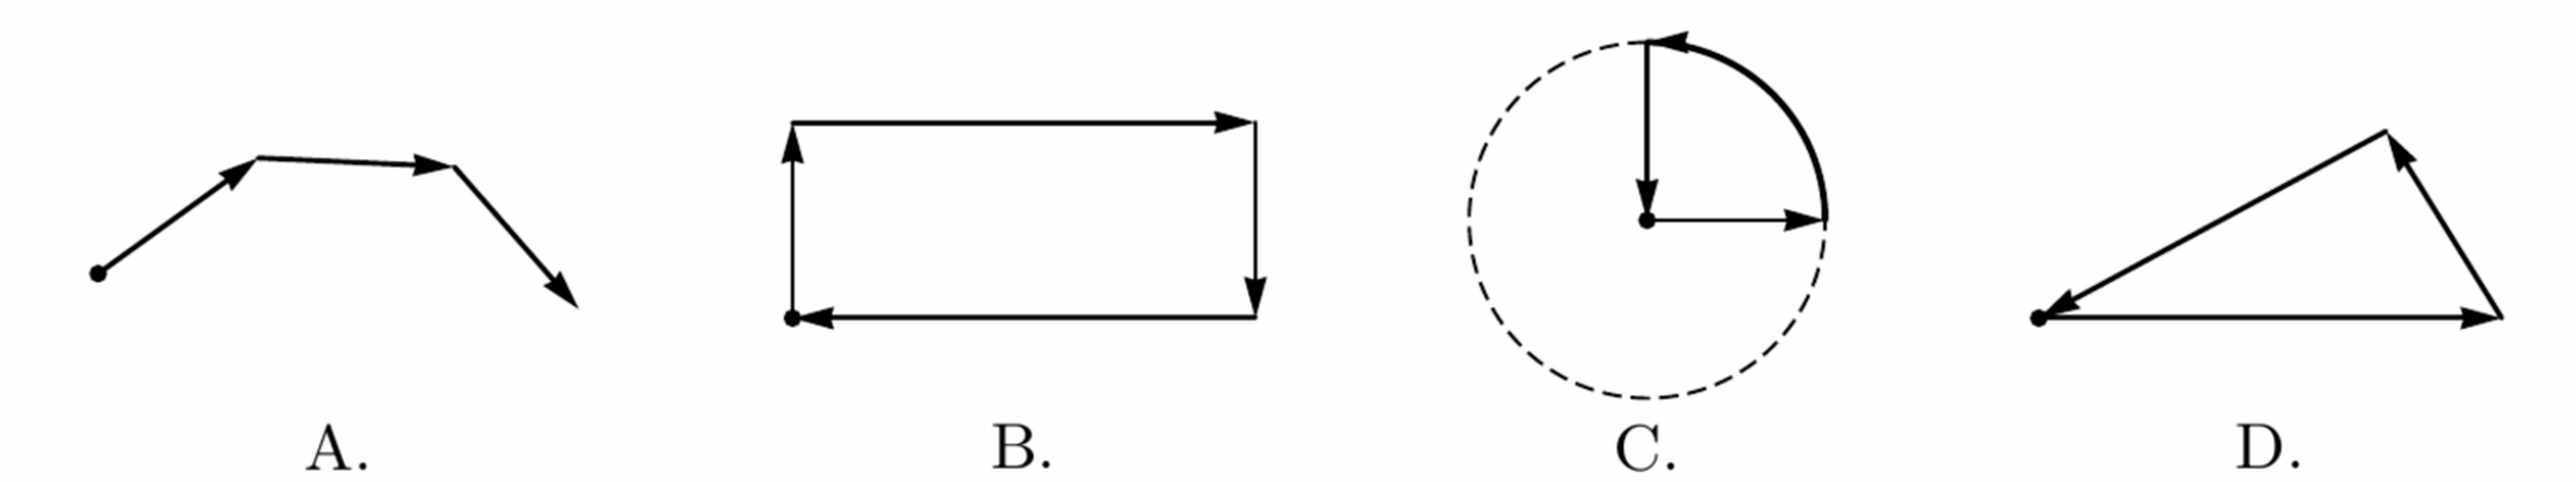
\includegraphics[width=0.86\textwidth]{figures/gao156_q14_opts.png}
\end{center}

\ifanswer
\solbegin
\step{由王老师锻炼时所走的离家距离（$S$）与行走时间（$t$）之间的函数关系图，}
\step{得在中间一段时间里，他到家的距离为定值，}
\step{故他所走的路程是一段以家为圆心的圆弧，故选 $C$.}
\solend
\fi

% === Q15 === 解析内曲线交点图（仅答案版出）；解析 4 行，故选 B
\item 已知 $a+2^a=b+\log_2 b=c+\log_3 c=k$，若 $k<1$，则\mbox{（\quad）}

\keepwithprev
A. $c<a<b$\qquad B. $a<c<b$\qquad C. $b<a<c$\qquad D. $a<b<c$

\ifanswer
\solbegin
\step{因为 $a+2^a=b+\log_2 b=c+\log_3 c=k$，}
\step{所以 $2^a=-a+k$，$\log_2 b=-b+k$，$\log_3 c=-c+k$，其中 $k<1$；}
\step{分别作出 $y=2^x$，$y=\log_2 x$，$y=\log_3 x$ 和 $y=-x+k$ 的图象，}

\begin{center}
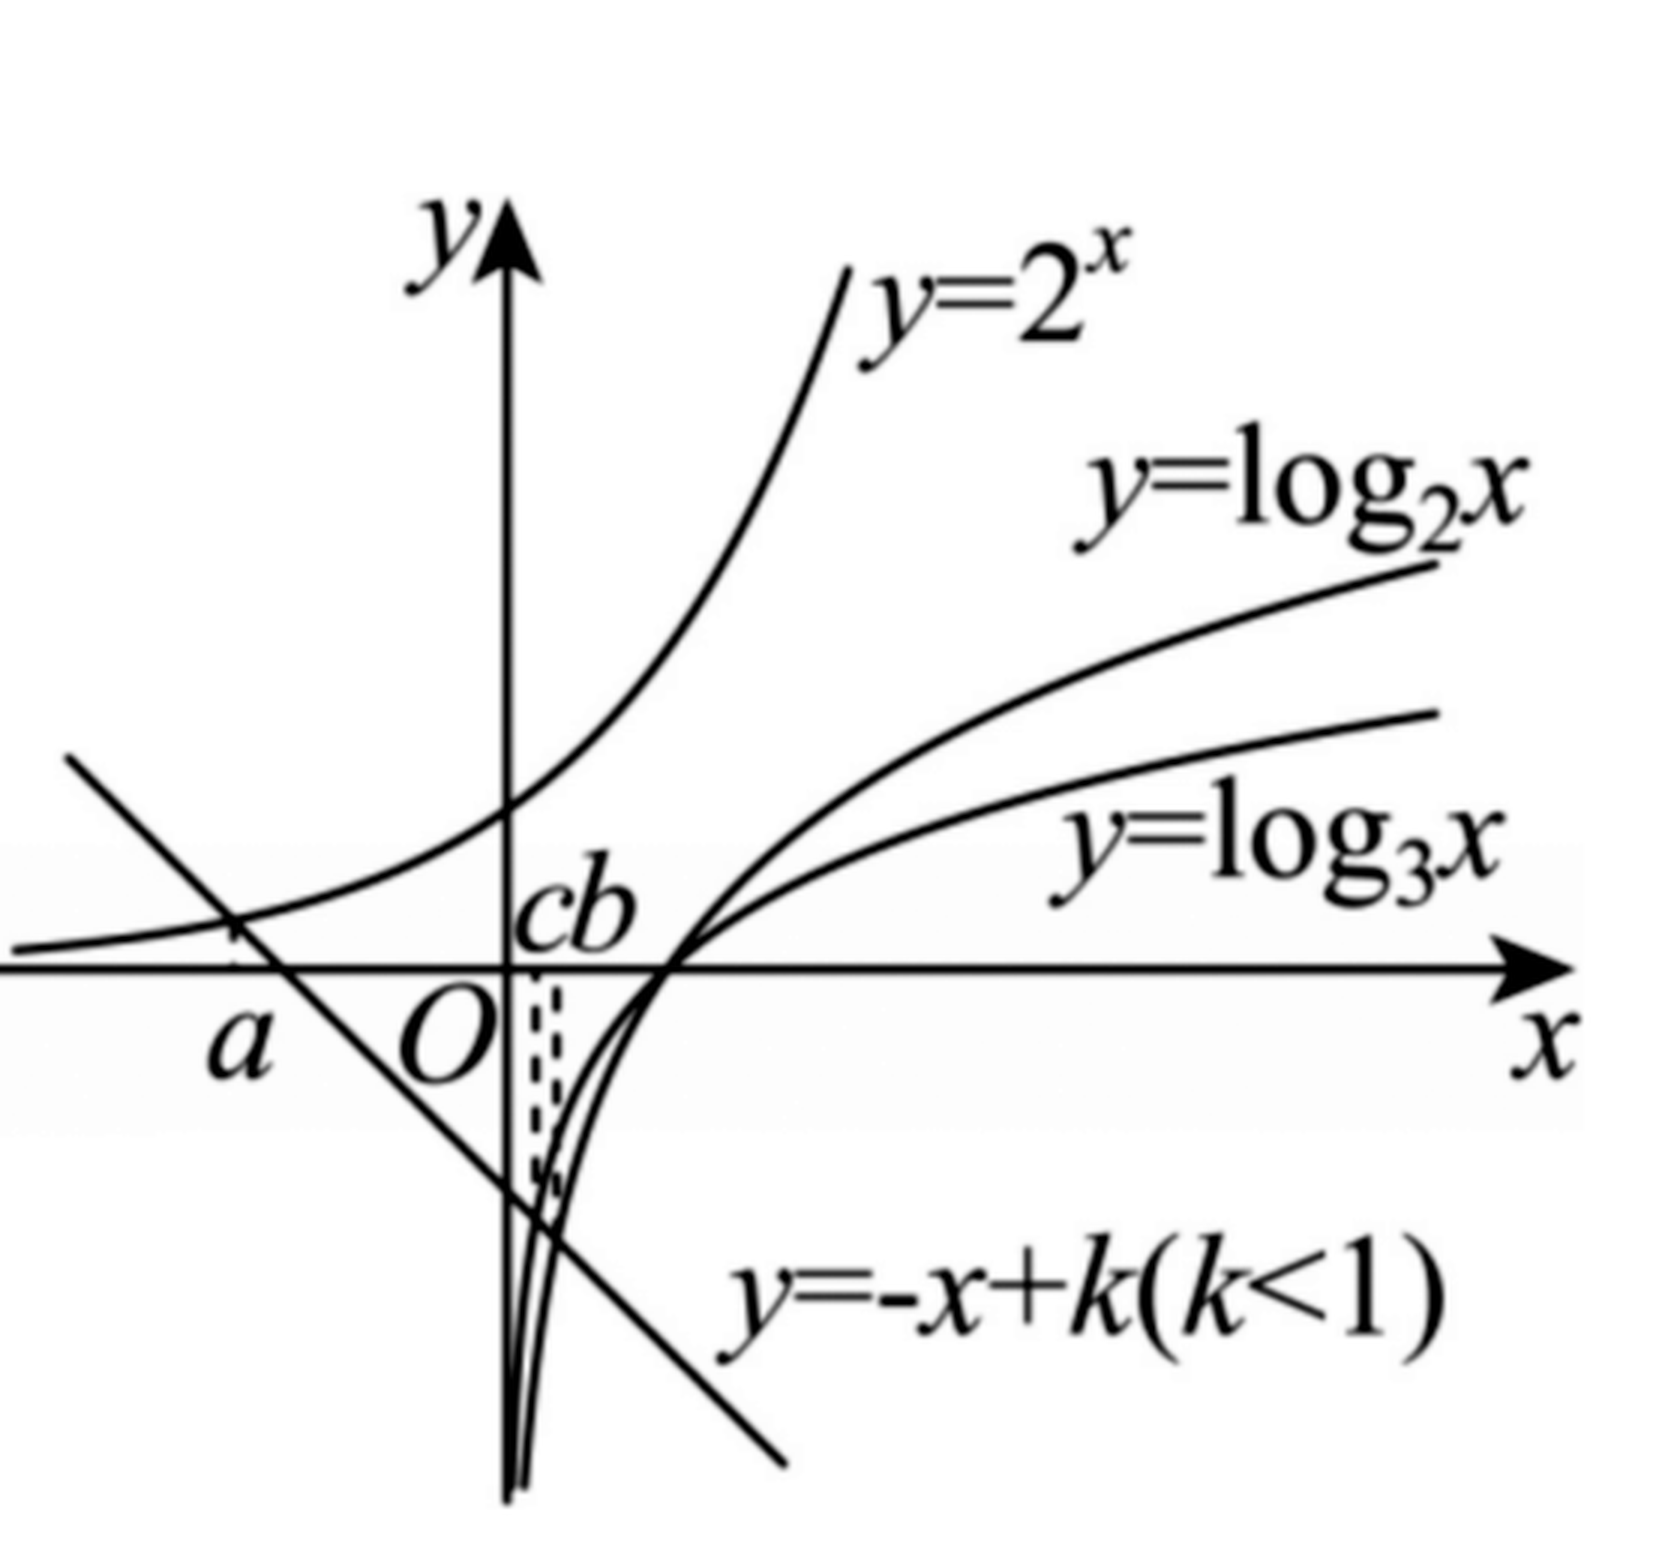
\includegraphics[width=0.52\textwidth]{figures/gao156_q15_curves.png}
\end{center}

\step{如图所示，由图象得 $a<c<b$. 故选 $B$.}
\solend
\fi

% === Q16 === ①② 文本圈数字、"一阶/二阶不动点""稳定点"自定义名词；解析 5 行，故选 A
\item 对定义域为 $I$ 的函数 $y=f(x)$，若存在 $x_0\in I$ 使得 $f(x_0)=x_0$，则称 $x_0$ 是函数 $f(x)$ 的
一阶不动点，简称不动点；若存在 $x_0\in I$ 使得 $f(f(x_0))=x_0$，则称 $x_0$ 是函数 $f(x)$ 的二阶
不动点，简称稳定点. 现有如下两个命题：①存在函数非 $y=x$ 且有无穷多个不动点；②
存在函数有无穷多个稳定点，且这些稳定点不都是不动点. 则\mbox{（\quad）}

\keepwithprev
A. ①成立，②成立\qquad\qquad B. ①成立，②不成立

C. ①不成立，②成立\qquad\qquad D. ①不成立，②不成立

\ifanswer
\solbegin
\step{①取定义在全体实数上的 $f(x)=\lvert x\rvert$，其不动点为一切非负实数，有无穷多个，}
\step{且 $f(-1)=1\ne-1$，①成立.}
\step{②取定义在全体实数上的 $g(x)=-x$，则 $g(g(x))=-(-x)=x$，}
\step{全体实数都是稳定点，而不动点只有 0，②成立.}
\step{故选 $A$.}
\solend
\fi

\end{enumerate}

\bigsec{三、解答题}

\begin{enumerate}
\setcounter{enumi}{16}

% === Q17 === $A\cap B$、$B\cap C$、\varnothing、\mid；解析 6 行
\item 设集合 $A=\{x\mid-1\leqslant x\leqslant2\}$，$B=\{x\mid2m<x<1\}$，$C=\{x\mid x<-1$ 或 $x>2\}$.

(1) 若 $A\cap B=B$，求实数 $m$ 的取值范围；

(2) 若 $B\cap C$ 中只有一个整数，求实数 $m$ 的取值范围.

\ifanswer
\solbegin
\step{(1) 当 $m\geqslant\dfrac12$ 时，$B=\varnothing$，满足 $A\cap B=B$.}
\step{当 $m<\dfrac12$ 时，$A\cap B=B$ 等价于 $2m\geqslant-1$，得 $-\dfrac12\leqslant m<\dfrac12$.}
\step{因此 $m$ 的取值范围为 $\left[-\dfrac12,+\infty\right)$.}
\step{(2) $B\cap C=\{x\mid2m<x<-1\}$，其中只有一个整数时，该整数必为 $-2$.}
\step{包含 $-2$ 且不包含 $-3$，等价于 $-3\leqslant2m<-2$，}
\step{因此 $m$ 的取值范围为 $\left[-\dfrac32,-1\right)$.}
\solend
\fi

% === Q18 === 幂函数 $x^{-\frac13}$、$m\in\R$；解析 12 行，跨 05—06 页
\item 已知幂函数 $f(x)=(3m^2-2m)x^m$（$m\in\R$）在定义域上不单调.

(1) 求函数 $f(x)$ 的解析式；

(2) 若 $f(a+1)<f(-2a+3)$，求实数 $a$ 的取值范围.

\ifanswer
\solbegin
\step{(1) 由幂函数的定义，$3m^2-2m=1$，即 $(3m+1)(m-1)=0$，得 $m=1$ 或 $m=-\dfrac13$.}
\step{当 $m=1$ 时，$f(x)=x$ 在定义域上单调递增，不合题意.}
\step{当 $m=-\dfrac13$ 时，$f(-1)=-1<f(1)=1$，而 $f(1)=1>f(8)=\dfrac12$，}
\step{故 $f(x)$ 在定义域上不单调.}
\step{因此 $f(x)=x^{-\frac13}$，定义域为 $(-\infty,0)\cup(0,+\infty)$.}
\step{(2) 有意义的条件为 $a\ne-1$ 且 $a\ne\dfrac32$.}
\step{当 $a<-1$ 时，$a+1<0<-2a+3$，有 $f(a+1)<0<f(-2a+3)$，}
\step{不等式成立.}
\step{当 $-1<a<\dfrac32$ 时，利用 $f(x)$ 在 $(0,+\infty)$ 上单调递减，}
\step{原不等式等价于 $a+1>-2a+3$，得 $\dfrac23<a<\dfrac32$.}
\step{当 $a>\dfrac32$ 时，$f(a+1)>0>f(-2a+3)$，不等式不成立.}
\step{所以 $a\in(-\infty,-1)\cup\left(\dfrac23,\dfrac32\right)$.}
\solend
\fi

% === Q19 === 两套解法（法一红字 \stepm，法二无标签）；\Delta 与 \subseteq；解析 21 行，跨 06—08 页
\item 已知 $a,c\in\R$，函数 $f(x)=\dfrac{x^2+(3a+1)x+c}{x+a}$.

(1) 若 $a=0$，求函数的定义域，并判断是否存在 $c$ 使得 $y=f(x)$ 图像关于原点对称，说明理由；

(2) 若函数过点 $(1,3)$，且函数 $y=f(x)$ 与 $x$ 轴负半轴有两个不同交点，求此时 $c$ 的值和 $a$ 的取值范围.

\ifanswer
\solbegin
\step{(1) 当 $a=0$ 时，$f(x)=\dfrac{x^2+(3a+1)x+c}{x+a}=\dfrac{x^2+x+c}{x}=x+\dfrac cx+1$，}
\step{故定义域为 $(-\infty,0)\cup(0,+\infty)$；}
\step{若存在实数 $c$，使得函数 $f(x)$ 为奇函数，则必有 $f(x)+f(-x)=0$，}
\step{而 $x+\dfrac cx+1+(-x)+\dfrac c{-x}+1=2\ne0$，}
\step{所以不存在实数 $c$，使得函数 $f(x)$ 为奇函数；}
\step{(2) 函数 $f(x)$ 的图像过点 $(1,3)$，则 $f(1)=\dfrac{1+(3a+1)+c}{1+a}=\dfrac{3a+c+2}{a+1}=3$，}
\step{解得 $c=1$，所以 $f(x)=\dfrac{x^2+(3a+1)x+1}{x+a}$，}
\stepm{法一：}{令 $f(x)=0$，则 $x^2+(3a+1)x+1=0$，此时方程有两不等负根，}
\step{则有 $\begin{cases}\Delta=(3a+1)^2-4>0\\-(3a+1)<0\end{cases}\Rightarrow\begin{cases}a>\dfrac13\text{ 或 }a<-1\\a>-\dfrac13\end{cases}\Rightarrow a>\dfrac13$，}
\step{注意到分母 $x+a\ne0$，则 $x\ne-a$，}
\step{若 $x=-a$ 也是方程 $x^2+(3a+1)x+1=0$ 的解，}
\step{代入方程 $(-a)^2+(3a+1)(-a)+1=0\Rightarrow2a^2+a-1=(a+1)(2a-1)=0$，}
\step{解得 $a=-1$ 或 $a=\dfrac12$，从而 $a\ne\dfrac12$，}
\step{综上，实数 $a$ 的取值范围为 $\left(\dfrac13,\dfrac12\right)\cup\left(\dfrac12,+\infty\right)$.}
\step{令 $g(x)=x^2+(3a+1)x+1$，与 $x$ 轴负半轴有两个交点，}
\step{则 $\begin{cases}-(3a+1)<0\\\Delta=(3a+1)^2-4>0\end{cases}\Rightarrow a>\dfrac13$.}
\step{注意到分母 $x+a\ne0$，则 $x\ne-a$，}
\step{若 $x=-a$ 也是方程 $x^2+(3a+1)x+1=0$ 的解，}
\step{代入方程 $(-a)^2+(3a+1)(-a)+1=0\Rightarrow2a^2+a-1=(a+1)(2a-1)=0$，}
\step{解得 $a=-1$ 或 $a=\dfrac12$，从而 $a\ne\dfrac12$，}
\step{综上，实数 $a$ 的取值范围为 $\left(\dfrac13,\dfrac12\right)\cup\left(\dfrac12,+\infty\right)$.}
\solend
\fi

% === Q20 === $Q$ 常数段 80000 照录；cases 与基本不等式；解析 10 行，跨 08—09 页
\item 某工厂生产某种零件的固定成本为 20000 元，每生产一个零件要增加投入 100 元，已知
总收入 $Q$（单位：元）关于产量 $x$（单位：个）满足函数：$Q=\begin{cases}400x-\dfrac12x^2,&0\leqslant x\leqslant400\\80000,&x>400\end{cases}$.

(1) 将利润 $P$（单位：元）表示为产量 $x$ 的函数；（总收入$=$总成本$+$利润）

(2) 当产量为何值时，零件的单位利润最大？最大单位利润是多少元？（单位利润$=$利润$\div$产量）

\ifanswer
\solbegin
\step{(1) 当 $0\leqslant x\leqslant400$ 时，}
\step{$P(x)=400x-\dfrac12x^2-20000-100x=-\dfrac12x^2+300x-20000$，}
\step{当 $x>400$ 时，$P(x)=80000-100x-20000=60000-100x$，}
\step{故 $P(x)=\begin{cases}-\dfrac12x^2+300x-20000,&0\leqslant x\leqslant400\\60000-100x,&x>400\end{cases}$.}
\step{(2) 设零件的单位利润为 $g(x)$，则 $g(x)=\begin{cases}-\dfrac12x-\dfrac{20000}{x}+300,&0\leqslant x\leqslant400\\\dfrac{60000}{x}-100,&x>400\end{cases}$，}
\step{当 $0\leqslant x\leqslant400$ 时，}
\step{$g(x)=300-\left(\dfrac12x+\dfrac{20000}{x}\right)\leqslant300-2\sqrt{\dfrac x2\cdot\dfrac{20000}{x}}=100$，}
\step{当且仅当 $\dfrac x2=\dfrac{20000}{x}$，即 $x=200$ 时取等号，}
\step{当 $x>400$ 时，$g(x)=\dfrac{60000}{x}-100$，此时无最值，}
\step{故当产量为 200 个，零件的单位利润最大，最大单位利润是 100 元.}
\solend
\fi

% === Q21 === 上升集定义、$D(x_0)=\{d\in\R\mid\cdots\}$、①②③ 文本圈数字、
%            \subseteq 带下划线、$-2^{-x}$；解析 19 行，跨 09—10 页
\item 已知函数 $y=f(x)$ 的定义域为 $\R$. 对任意 $x_0\in\R$，定义集合
$D(x_0)=\{d\in\R\mid f(x_0+d)>f(x_0)\}$，则称 $D(x_0)$ 为函数 $y=f(x)$ 在 $x_0$ 处的上升集.

(1) 若 $f(x)=1-x$，求 $D(-1)$；

(2) 若 $f(x)=\begin{cases}2^x,&x<0\\0,&x=0\\-2^{-x},&x>0\end{cases}$，求 $D(x)$；

(3) 设 $y=f(x)$ 满足：①当 $x<0$ 时，$f(x)=2^x$；②若 $f(x_1)\leqslant f(x_2)$，则
$D(x_2)\subseteq D(x_1)$；③当 $0<x<1$ 时，$f(x)<f(0)$. 证明：$f(0)\geqslant1$.

\ifanswer
\solbegin
\step{(1) $f(-1+d)>f(-1)\Leftrightarrow2-d>2\Leftrightarrow d<0$，所以 $D(-1)=(-\infty,0)$.}
\step{(2) 函数在 $(-\infty,0)$、$(0,+\infty)$ 上分别严格递增，}
\step{且这两个区间上的函数值分别为正、负，$f(0)=0$.}
\step{当 $x<0$ 时，$f(x+d)>f(x)\Leftrightarrow x<x+d<0\Leftrightarrow0<d<-x$，}
\step{当 $x=0$ 时，$f(d)>f(0)\Leftrightarrow d<0$，}
\step{当 $x>0$ 时，$f(x+d)>f(x)\Leftrightarrow x+d\leqslant0$ 或 $x+d>x$}
\step{$\Leftrightarrow d\leqslant-x$ 或 $d>0$，}
\step{因此 $D(x)=\begin{cases}(0,-x),&x<0\\(-\infty,0),&x=0\\(-\infty,-x]\cup(0,+\infty),&x>0\end{cases}$.}
\step{(3) 任取 $a\in(-1,0)$，}
\step{令 $d=-\dfrac a2$，则 $0<d<1$，且 $f(a+d)=2^{\frac a2}>2^a=f(a)$，}
\step{所以 $d\in D(a)$；}
\step{由③，$f(d)<f(0)$，所以 $d\notin D(0)$.}
\step{若 $f(0)\leqslant f(a)$，由②得 $D(a)\subseteq D(0)$，与上述结论矛盾.}
\step{因此，对任意 $a\in(-1,0)$，都有 $f(0)>2^a$.}
\step{特别地 $f(0)>2^{-\frac12}>0$.}
\step{若 $f(0)<1$，取 $a=\dfrac12\log_2 f(0)$，则 $-\dfrac14<a<0$，且}
\step{$2^a=\sqrt{f(0)}>f(0)$，}
\step{与 $f(0)>2^a$ 矛盾.}
\step{所以 $f(0)\geqslant1$.}
\solend
\fi

\end{enumerate}

\end{document}
"
%
% ① 原始材料：微信公众号"魔都数学加油站"文章，连载"27学年高一156"，原文标题
% "27学年高一156——2026-2027年上海市大同中学高一上期中"；
% 原文链接：https://mp.weixin.qq.com/s/xLtS5tyjCPJIWCIBohwGvw 。
% 正文为 10 张 PNG 页（01/02/03/04/05/06/07/08/09/10 各页分辨率混排
% 2560×3620 与 4762×6735，逐页按各自分辨率裁图核对）。
% 体例：讲评版——填空 3—12（10 题）、选择 13—16（4 题）、解答 17—21（5 题），
% 共 19 题，自第 3 题起编（1、2 未印在本篇）；Q3 只印【答案】、其余 18 题
% 逐题印【解析】（逐题核实，见 ②）。题目、答案、解析均据原图转录；卷面粉红色
% 水印"魔都数学加油站"及公众号页脚未录入。
%
% 卷首标题：原卷印作"2026-2027 年大同中学高一上期中"，年份区间按全稿惯例排 en dash；
% 原卷卷面未印副标题，本稿按同期中卷知识模块口径补出"集合与常用逻辑用语、不等式、函数"。
%
% ② 与原卷的排版差异：
%   ① 原文从第 3 题起，本稿保留原题号；共 19 题三节，解答题 5 题到 21；
%   ② 混合体例：第 3 题只印【答案】、无【解析】，按 高一140 第 5 题／高一145
%      第 3 题／高一151 第 7 题成例另提 \ans{}、不补造解析；其余 18 题印
%      【解析】、用 \solbegin…\solend；四道选择题答案在解析末句"故选 C／C／B／A"
%      （逐个放大复核）、括号 \mbox{（\quad）} 留空、不另提 \ans{}；答案版
%      【答案】/【解析】标记数 = 19 = 全卷题数（1 个 \ans ＋ 18 个 \solbegin）；
%   ③ 原卷卷面未印副标题，本稿按知识模块口径补出；
%   ④ 原卷填空横线按全稿惯例排 \blankline[4.4em]；选择题括号排 \mbox{（\quad）}、
%      选项段前按惯例各加 \keepwithprev；解答题不留作答区、不加 \anspace
%      （原卷为讲评版，109—113 起全稿不用 \anspace）；
%   ⑤ 数集：Q3"$x\in\R$"、Q18"$m\in\R$"、Q19"$a,c\in\R$"、Q21"定义域为 \R"
%      "任意 $x_0\in\R$""$d\in\R$"原卷印正体粗体 R，按全稿惯例归一 \R；
%      绝对值排 \lvert…\rvert（Q11 $\lvert2^x-1\rvert$、Q16 $\lvert x\rvert$），
%      集合描述竖线排 \mid（Q17 $A=\{x\mid\cdots\}$、Q21 $D(x_0)=\{d\in\R\mid\cdots\}$），
%      空集 \varnothing（Q17"$B=\varnothing$"），不等号按全稿惯例排 \leqslant／\geqslant；
%   ⑥ 子集符号逐处照录不统一：Q21 (3) 题干"$D(x_2)\subseteq D(x_1)$"与解析
%      "$D(a)\subseteq D(0)$"均印带下划线 ⊆，照录 \subseteq；本卷无单线 ⊂ 用例；
%   ⑦ 判别式：Q19 两套解法"$\Delta=(3a+1)^2-4>0$"印等腰偏高 \Delta，照录 \Delta；
%      本卷无扁三角 \triangle 用例；
%   ⑧ 红字照录为黑体：Q19 (2) 解析第一套解法行首"法一："原卷排**红色加粗**，
%      按 高一53 成例排 \stepm{法一：}{…}（加粗着色、不改黑色基调），全库无红字
%      排字先例、本稿不引入红色定义，文件头注明；第二套解法原卷直接以
%      "令 $g(x)=x^2+(3a+1)x+1$，与 $x$ 轴负半轴有两个交点，"另起，
%      **未印"法二："标签**（逐页像素级复核：07 页仅 1437—1475 一处红字，
%      08 页无红字），照录为普通 \step、不补造标签；
%   ⑨ 文本模式圈数字逐处照录：Q12 解析 ①② 两情形、Q16 两则命题与四个选项及
%      解析的 ①②、Q21 (3) 三条件 ①②③ 与解析"由③""由②"，均为印刷圈数字
%      （非 \textcircled、非数学模式），计入圈数字实测；
%   ⑩ 自定义名词照录：Q16"一阶不动点，简称不动点""二阶不动点，简称稳定点"、
%      Q21"上升集"；Q16 题干"存在函数非 $y=x$ 且有无穷多个不动点"照录；
%   ⑪ 中文弯引号照录：Q3""存在 $x\in\R$，$x^3-1\leqslant0$" 否定形式为"、
%      Q13"使"$\dfrac{x+1}{1-x}\geqslant0$"成立的必要不充分条件是"；
%      注释里一律 ASCII 引号；数学式内 CJK 用 \text{}（Q19 cases 内"或"）；
%   ⑫ 半角逗号在数学组之间是全稿惯例、非笔误，逐处照录（$a,c$、$x,y$、$a,b$
%      之类）；行末西文句点 ASCII `.`；行中全角逗号／顿号照录；
%   ⑬ 复杂式照录别简化：Q6 $\left(\dfrac{1}{\sqrt a}\right)^{\frac27}\cdot\sqrt[7]{a^3}$
%      与解析 $a^{\frac{12}{7}-\frac17+\frac37}$、Q8 $2\sqrt4+5=9$（$\sqrt4$ 未化简）、
%      Q9 $\left(\sqrt x+\dfrac{1}{\sqrt x}\right)^3$、Q12 $\dfrac{4a-(2-a)^2}{4a}$、
%      Q18 $f(8)=\dfrac12$、Q19 $2a^2+a-1=(a+1)(2a-1)=0$、Q20 $Q$ 的常数段
%      $80000$（不是 $80000-100x$）与 $2\sqrt{\dfrac x2\cdot\dfrac{20000}{x}}$、
%      Q21 $f(a+d)=2^{\frac a2}>2^a=f(a)$ 与 $2^a=\sqrt{f(0)}>f(0)$ 等；
%      \left…\right 不得拆到不同 $…$ 组（Q5 $\left(0,\dfrac12\right)$、
%      Q12 $\left[0,4+2\sqrt3\right)$、Q17 $\left[-\dfrac12,+\infty\right)$、
%      Q19 $\left(\dfrac13,\dfrac12\right)\cup\left(\dfrac12,+\infty\right)$、
%      Q20 $\left(\dfrac12x+\dfrac{20000}{x}\right)$ 等）；cases 块整体算一个印刷行；
%   ⑭ 一条 \step = 原卷解析的一个印刷行；别并折行、别拆行。跨页续印按题合并
%      （Q6 的 01 页上下题干重复印、Q8 的 01—02 页、Q12 的 02—03 页、
%      Q15 的 04 页上下、Q16 的 04—05 页、Q17 的 05 页上下、Q18 的 05—06 页、
%      Q19 的 06—08 页、Q20 的 08—09 页、Q21 的 09—10 页）；
%      跨半页重叠行（Q12 的"②若 …"、Q18 的"原不等式等价于 …"、
%      Q20 的"【解析】(1) 当 $0\leqslant x\leqslant400$ 时，"、Q21 的
%      "【解析】(1) $f(-1+d)>f(-1)\cdots$"与"与 $f(0)>2^a$ 矛盾."）
%      只算一个印刷行；
%   ⑮ 配图：全卷 3 组（逐页通读 10 页确认）——
%      · Q14 题干 S-t 梯形图（03 页右下，离家距离 S 对行走时间 t），题目配图、
%        三版都出，裁 figures/gao156_q14_st.png；
%      · Q14 四幅路线选项（04 页上部，A/B/C/D 四幅横排、C 为以家为圆心的圆弧），
%        题目配图、三版都出，合并成一张，裁 figures/gao156_q14_opts.png；
%      · Q15 解析内曲线交点图（04 页右下，$y=2^x$、$y=\log_2x$、$y=\log_3x$
%        与 $y=-x+k$），仅答案版出，裁 figures/gao156_q15_curves.png；
%      3 图均取自原卷截图，去粉色水印、去色、3×~4× LANCZOS 放大；
%      Q14 题干"题干＋两图"整块用 \needvspace 守卫推走（守卫放 \item 之前，
%      见 高一154 Q15／高一136 Q13 成例）；Q15 解析内图放 \ifanswer 内
%      \solbegin…\solend 的两 \step 之间（高一108 第 6 题／高一154 附加题 2 成例）；
%      其余各页逐页确认无其它题目配图、无解析配图、无表格；10 页下半仅水印、无正文。
%
% ③ 行数复核：一条 \step = 原卷解析的一个印刷行，cases 块作一个印刷行计。
%   逐题数（主会话逐页核对定稿）：Q3：0（只印【答案】、提 \ans{}，不计入 \step 账）；
%   Q4：1；Q5：1；Q6：1；Q7：1；Q8：3；Q9：2；Q10：2；Q11：5；Q12：12；
%   Q13：3；Q14：3；Q15：4；Q16：5；Q17：6；Q18：12；Q19：21；Q20：10；Q21：19。
%   合计 111 行（110 条 \step ＋ 1 条 \stepm），与原卷逐题印刷行相等。
%   全卷 19 题：Q3 一处 \ans{} ＋ 其余 18 题设 \solbegin…\solend，
%   答案版【答案】/【解析】标记数 = 19 = 全卷题数。
%
% ④ 页码分布（供回原图复核）：
%   卷首标题＋"一、填空题"＋Q3 题干＋【答案】、Q4 题干＋解析 1 行、
%   Q5 题干＋解析 1 行、Q6 题干首行在 01 页上半；
%   Q6 题干（重复印）＋解析 1 行、Q7 题干＋解析 1 行、Q8 题干＋解析前 2 行
%   在 01 页下半；Q8 解析末行、Q9 题干＋解析 2 行、Q10 题干＋解析 2 行、
%   Q11 题干首行在 02 页上半；Q11 题干（重复印）＋解析 5 行、
%   Q12 题干＋解析首行在 02 页下半；Q12 解析中 9 行在 03 页上半；
%   Q12 解析末 2 行＋"二、选择题"标题＋Q13 题干＋选项＋解析 3 行＋
%   Q14 题干首行在 03 页下半；Q14 题干续行＋四幅选项图＋解析 3 行＋
%   Q15 题干＋选项＋解析前 2 行＋Q16 题干在 04 页上半；
%   Q15 解析后 2 行＋曲线图＋Q16 选项＋解析前 2 行在 04 页下半；
%   Q16 解析后 3 行＋"三、解答题"标题＋Q17 题干＋两问＋解析 (1) 3 行
%   在 05 页上半；Q17 解析 (2) 3 行＋Q18 题干＋两问＋解析 (1) 首 2 行
%   在 05 页下半；Q18 解析 (1)(2) 中 8 行在 06 页上半；Q18 解析末 2 行＋
%   Q19 题干＋两问＋解析 (1) 首行在 06 页下半；Q19 解析 (1) 后 4 行＋
%   (2) 前 2 行＋法一 2 行在 07 页上半；法一后 5 行＋法二前 3 行在 07 页下半；
%   法二后 4 行＋Q20 题干＋两问＋解析 (1) 首行在 08 页上半；
%   Q20 解析 (1) 后 3 行＋(2) 前 5 行在 08 页下半；Q20 解析 (2) 末 2 行＋
%   Q21 题干＋三问＋解析 (1) 首行在 09 页上半；Q21 解析 (1)（重复印）＋
%   (2) 8 行＋(3) 首行在 09 页下半；Q21 (3) 解析中 8 行在 10 页上半；
%   Q21 (3) 末 2 行在 10 页下半。本稿按题连排，不丢行、不并折行；
%   全卷末题为第 21 题，无附加题节。
%
\documentclass[a4paper,11pt]{article}
\usepackage{common}

\begin{document}

\examtitlest[3]{2026--2027 年大同中学高一上期中}{集合与常用逻辑用语、不等式、函数}

\bigsec{一、填空题}

\begin{enumerate}
\setcounter{enumi}{2}

% === Q3 === 只印【答案】、无【解析】；R 正体粗体 \R；中文弯引号照录
\item “存在 $x\in\R$，$x^3-1\leqslant0$” 否定形式为\blankline[4.4em].

\ifanswer
\ans{对任意 $x\in\R$，$x^3-1>0$}
\fi

% === Q4 === 解析 1 行
\item 若实数 $a>0$ 且 $a\ne1$，函数 $y=a^{x-3}+1$ 的图像恒过定点 $P$，则点 $P$ 的坐标为\blankline[4.4em].

\ifanswer
\solbegin
\step{当 $x=3$ 时，$y=a^0+1=2$，与 $a$ 无关，所以定点为 $P(3,2)$.}
\solend
\fi

% === Q5 === 解析 1 行
\item 函数 $y=\dfrac{1}{3^x+2}$ 的值域是\blankline[4.4em].

\ifanswer
\solbegin
\step{$3^x\in(0,+\infty)$，因此 $3^x+2\in(2,+\infty)$，值域为 $\left(0,\dfrac12\right)$.}
\solend
\fi

% === Q6 === 根式嵌套照录；解析 1 行；题干跨 01 页上下重复印
\item 已知 $a>0$，化简 $a^{\frac{12}{7}}\cdot\left(\dfrac{1}{\sqrt a}\right)^{\frac27}\cdot\sqrt[7]{a^3}=$\blankline[4.4em].

\ifanswer
\solbegin
\step{原式 $=a^{\frac{12}{7}}\cdot a^{-\frac17}\cdot a^{\frac37}=a^{\frac{12}{7}-\frac17+\frac37}=a^2$.}
\solend
\fi

% === Q7 === 换底公式；解析 1 行
\item 已知 $\log_5 3=a$，用 $a$ 的代数式表示 $\log_{15}125=$\blankline[4.4em].

\ifanswer
\solbegin
\step{$\log_{15}125=\dfrac{\log_5 125}{\log_5 15}=\dfrac{3}{1+\log_5 3}=\dfrac{3}{1+a}$.}
\solend
\fi

% === Q8 === 基本不等式，$\sqrt4$ 照录未化简；解析 3 行，跨 01—02 页
\item 已知 $x>0$，$y>0$，且 $4x+y=xy$，则 $x+y$ 的最小值为\blankline[4.4em].

\ifanswer
\solbegin
\step{由 $4x+y=xy$，得 $\dfrac4y+\dfrac1x=1$，}
\step{则 $x+y=(x+y)\left(\dfrac4y+\dfrac1x\right)=\dfrac{4x}{y}+\dfrac yx+1+4\geqslant2\sqrt4+5=9$，}
\step{当且仅当 $\dfrac{4x}{y}=\dfrac yx$，即 $x=3$，$y=6$ 时取等号，故最小值为 9.}
\solend
\fi

% === Q9 === 解析 2 行
\item 已知 $x^{-1}+x=7$（$x>0$），则 $x^{\frac32}+x^{-\frac32}$ 的值为\blankline[4.4em].

\ifanswer
\solbegin
\step{$x>0$，有 $\sqrt x+\dfrac{1}{\sqrt x}=\sqrt{x+\dfrac1x+2}=3$，}
\step{所以 $x^{\frac32}+x^{-\frac32}=\left(\sqrt x+\dfrac{1}{\sqrt x}\right)^3-3\left(\sqrt x+\dfrac{1}{\sqrt x}\right)=27-9=18$.}
\solend
\fi

% === Q10 === $x_{\min}$；解析 2 行
\item 已知不等式 $x>\dfrac{2a+1}{a-1}$ 对任意的 $x\in[1,2]$ 恒成立，则实数 $a$ 的取值范围是\blankline[4.4em].

\ifanswer
\solbegin
\step{不等式 $x>\dfrac{2a+1}{a-1}$ 对任意的 $x\in[1,2]$ 恒成立，得 $\dfrac{2a+1}{a-1}<x_{\min}=1$，}
\step{即有 $\dfrac{a+2}{a-1}<0$，解得 $-2<a<1$，则实数 $a$ 的取值范围是 $(-2,1)$.}
\solend
\fi

% === Q11 === 分段函数 cases 与绝对值 \lvert…\rvert；解析 5 行
\item 已知函数 $f(x)=\begin{cases}\lvert2^x-1\rvert-a,&x\leqslant2\\\dfrac{3}{x-1}-a,&x>2\end{cases}$，若函数 $y=f(x)$ 图像与 $x$ 轴有三个不同交点，则实数 $a$ 的取值范围是\blankline[4.4em].

\ifanswer
\solbegin
\step{令 $g(x)=f(x)+a$.}
\step{在 $(-\infty,0)$、$[0,2]$、$(2,+\infty)$ 上，$g(x)$ 均严格单调，}
\step{值域依次为 $(0,1)$、$[0,3]$、$(0,3)$.}
\step{每段至多有一个交点，因而恰有三个不同交点，}
\step{当且仅当 $a\in(0,1)\cap[0,3]\cap(0,3)=(0,1)$.}
\solend
\fi

% === Q12 === ①② 文本圈数字、对称轴与最小值式照录；解析 12 行，跨 02—03 页
\item 已知函数 $f(x)=ax^2-(2-a)x+1$，$g(x)=x$，若对于任意实数 $x$，$f(x)$ 与 $g(x)$ 至少有一个为正数，则实数 $a$ 的取值范围是\blankline[4.4em].

\ifanswer
\solbegin
\step{当 $x>0$ 时，$g(x)>0$；当 $x<0$ 时，$g(x)<0$；}
\step{当 $x=0$ 时，$f(0)=1>0$；}
\step{因为对于任意实数 $x$，$f(x)$ 与 $g(x)$ 至少有一个为正数，}
\step{当 $x<0$ 时，因为 $g(x)<0$，所以 $f(x)=ax^2-(2-a)x+1>0$ 恒成立，}
\step{当 $a<0$ 时，显然不成立，}
\step{当 $a=0$ 时，$f(x)=-2x+1>0$，对 $x<0$ 时恒成立，满足题意，}
\step{当 $a>0$ 时，函数图象开口向上，对称轴 $x=\dfrac{2-a}{2a}$，}
\step{①若 $\dfrac{2-a}{2a}\geqslant0$，即 $0<a\leqslant2$ 时，函数 $f(x)$ 在 $(-\infty,0)$ 上严格减，$f(0)=1$，}
\step{故 $f(x)>0$ 对 $x<0$ 时恒成立，满足题意；}
\step{②若 $\dfrac{2-a}{2a}<0$，即 $a>2$ 时，$f(x)_{\min}=f\left(\dfrac{2-a}{2a}\right)=\dfrac{4a-(2-a)^2}{4a}>0$，}
\step{解得 $4-2\sqrt3<a<4+2\sqrt3$，所以 $2<a<4+2\sqrt3$.}
\step{综上，$0\leqslant a<4+2\sqrt3$，故实数 $a$ 的取值范围是 $\left[0,4+2\sqrt3\right)$.}
\solend
\fi

\end{enumerate}

\bigsec{二、选择题}

\begin{enumerate}
\setcounter{enumi}{12}

% === Q13 === 必要不充分条件；cases 块；解析 3 行，故选 C
\item 使 “$\dfrac{x+1}{1-x}\geqslant0$” 成立的必要不充分条件是\mbox{（\quad）}

\keepwithprev
A. $-1\leqslant x<1$\qquad B. $x\leqslant-1$ 或 $x>1$\qquad C. $-1\leqslant x\leqslant1$\qquad D. $x\leqslant-1$ 或 $x\geqslant0$

\ifanswer
\solbegin
\step{由不等式 $\dfrac{x+1}{1-x}\geqslant0$ 得 $\begin{cases}(x+1)(1-x)\geqslant0\\1-x\ne0\end{cases}$，解得 $-1\leqslant x<1$，}
\step{由题意结合选项，$-1\leqslant x<1\Rightarrow-1\leqslant x\leqslant1$ 成立，反之不成立，}
\step{所以 $-1\leqslant x\leqslant1$ 是 $\dfrac{x+1}{1-x}\geqslant0$ 成立的必要不充分条件. 故选 $C$.}
\solend
\fi

% === Q14 === 题干 S-t 图＋四幅路线选项（题目配图，三版都出）；守卫放 \item 之前；解析 3 行，故选 C
\needvspace{9cm}
\item 如图是王老师锻炼时所走的离家距离（$S$）与行走时间（$t$）之间的函数关系图，若
用黑点表示王老师家的位置，则王老师行走的路线可能是\mbox{（\quad）}

\begin{center}
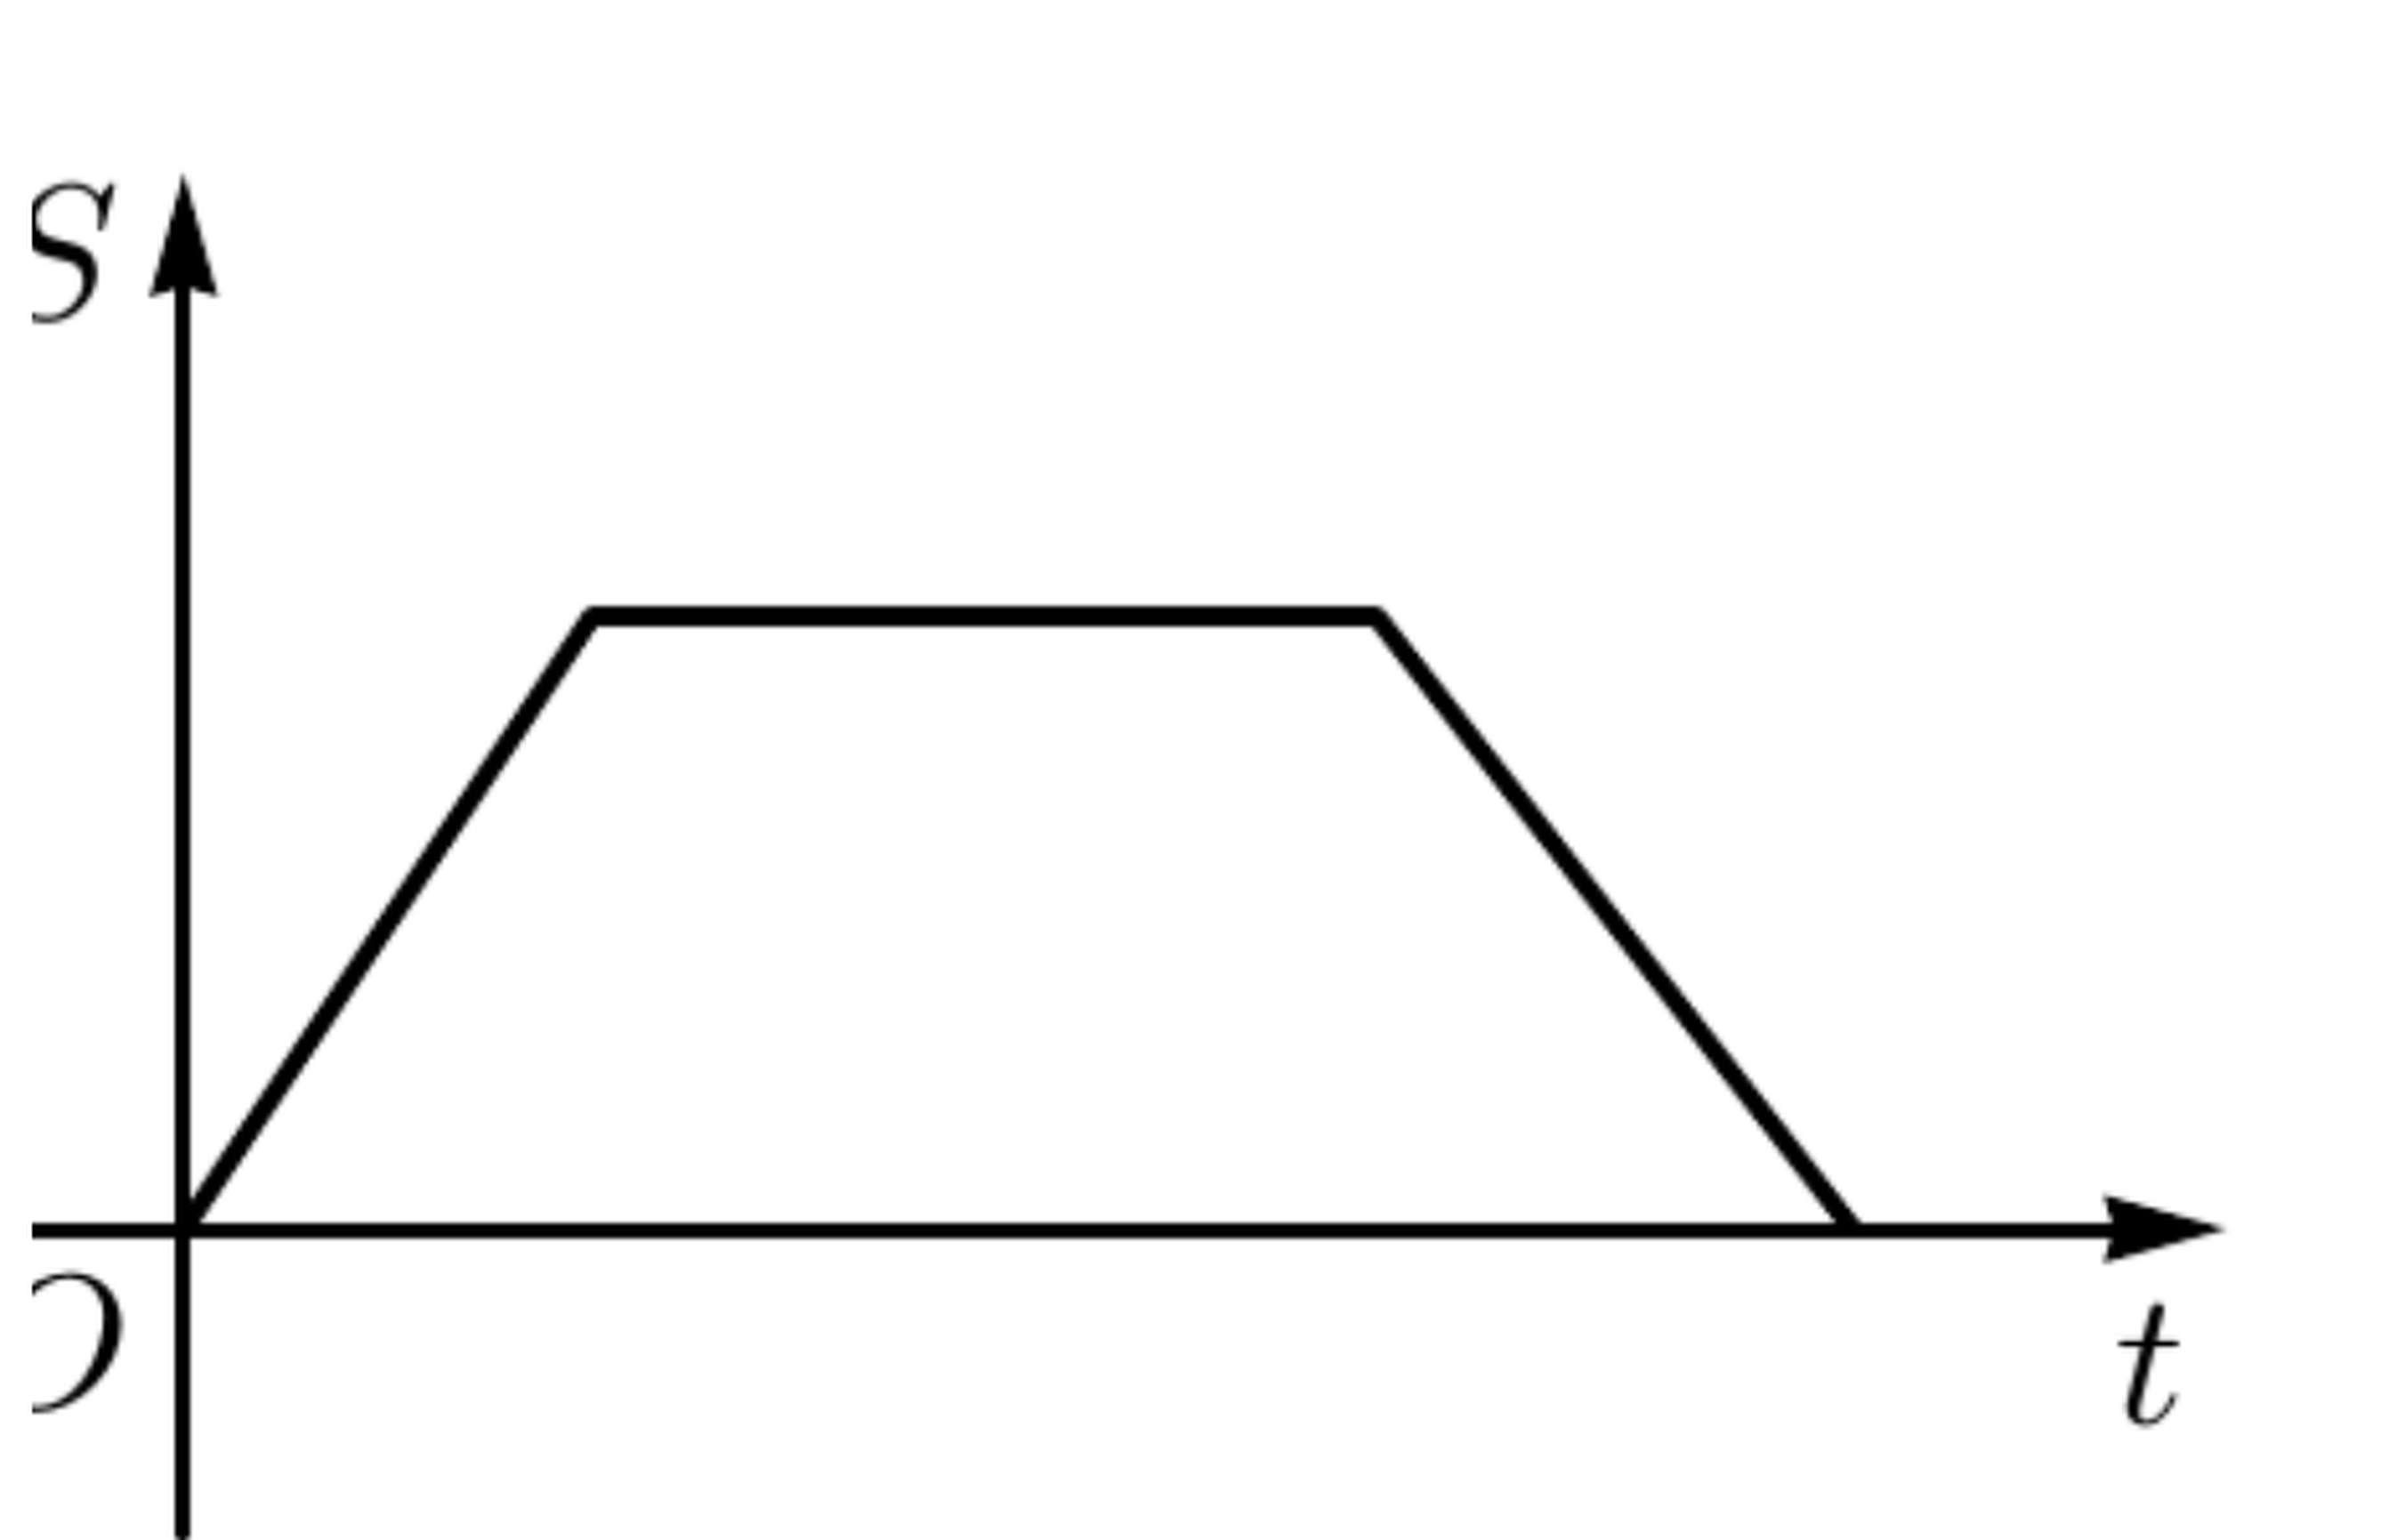
\includegraphics[width=0.34\textwidth]{figures/gao156_q14_st.png}
\end{center}

\keepwithprev
\begin{center}
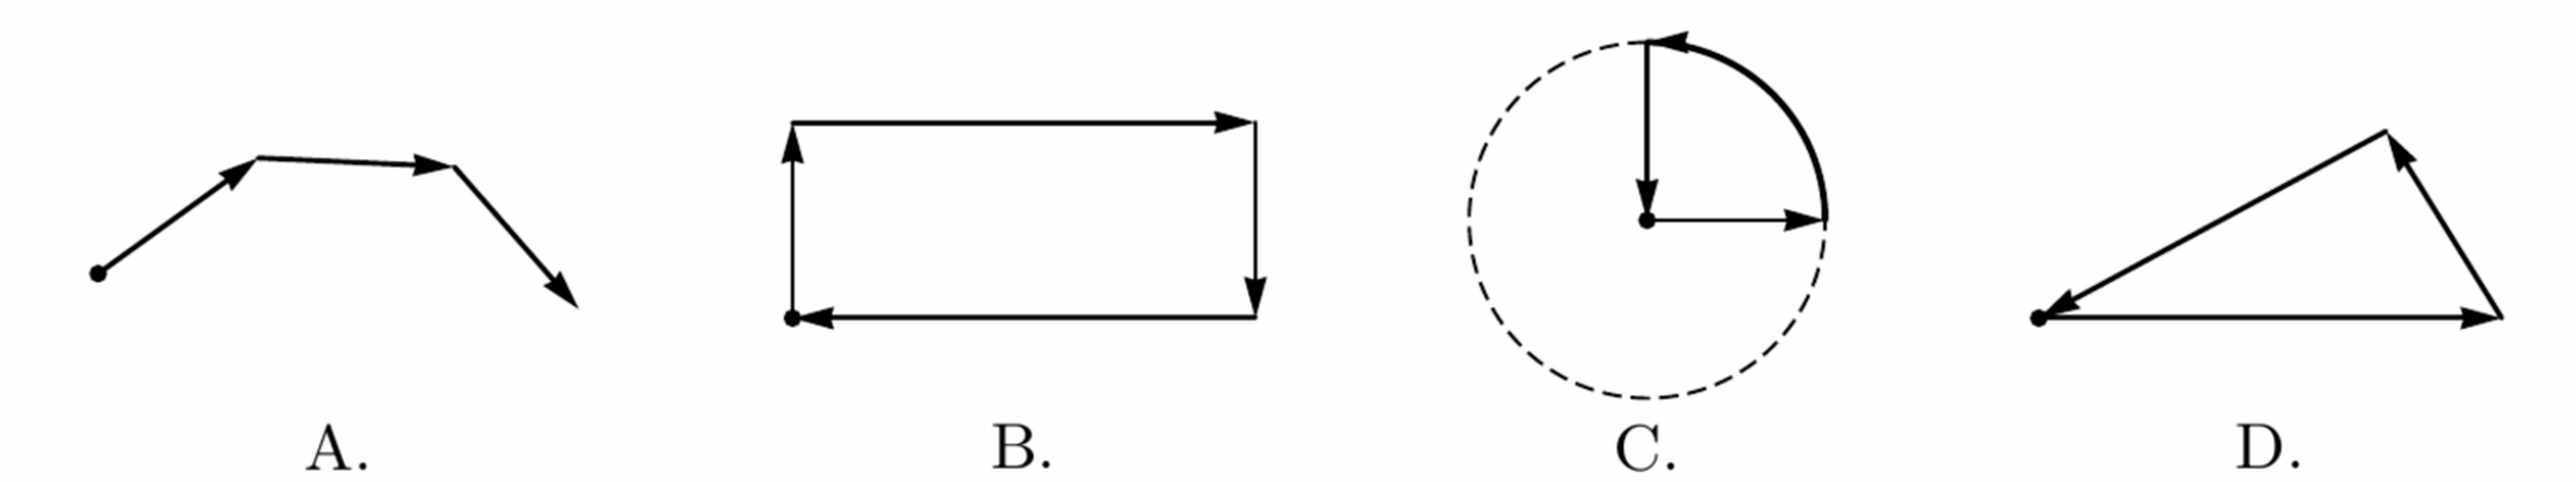
\includegraphics[width=0.86\textwidth]{figures/gao156_q14_opts.png}
\end{center}

\ifanswer
\solbegin
\step{由王老师锻炼时所走的离家距离（$S$）与行走时间（$t$）之间的函数关系图，}
\step{得在中间一段时间里，他到家的距离为定值，}
\step{故他所走的路程是一段以家为圆心的圆弧，故选 $C$.}
\solend
\fi

% === Q15 === 解析内曲线交点图（仅答案版出）；解析 4 行，故选 B
\item 已知 $a+2^a=b+\log_2 b=c+\log_3 c=k$，若 $k<1$，则\mbox{（\quad）}

\keepwithprev
A. $c<a<b$\qquad B. $a<c<b$\qquad C. $b<a<c$\qquad D. $a<b<c$

\ifanswer
\solbegin
\step{因为 $a+2^a=b+\log_2 b=c+\log_3 c=k$，}
\step{所以 $2^a=-a+k$，$\log_2 b=-b+k$，$\log_3 c=-c+k$，其中 $k<1$；}
\step{分别作出 $y=2^x$，$y=\log_2 x$，$y=\log_3 x$ 和 $y=-x+k$ 的图象，}

\begin{center}
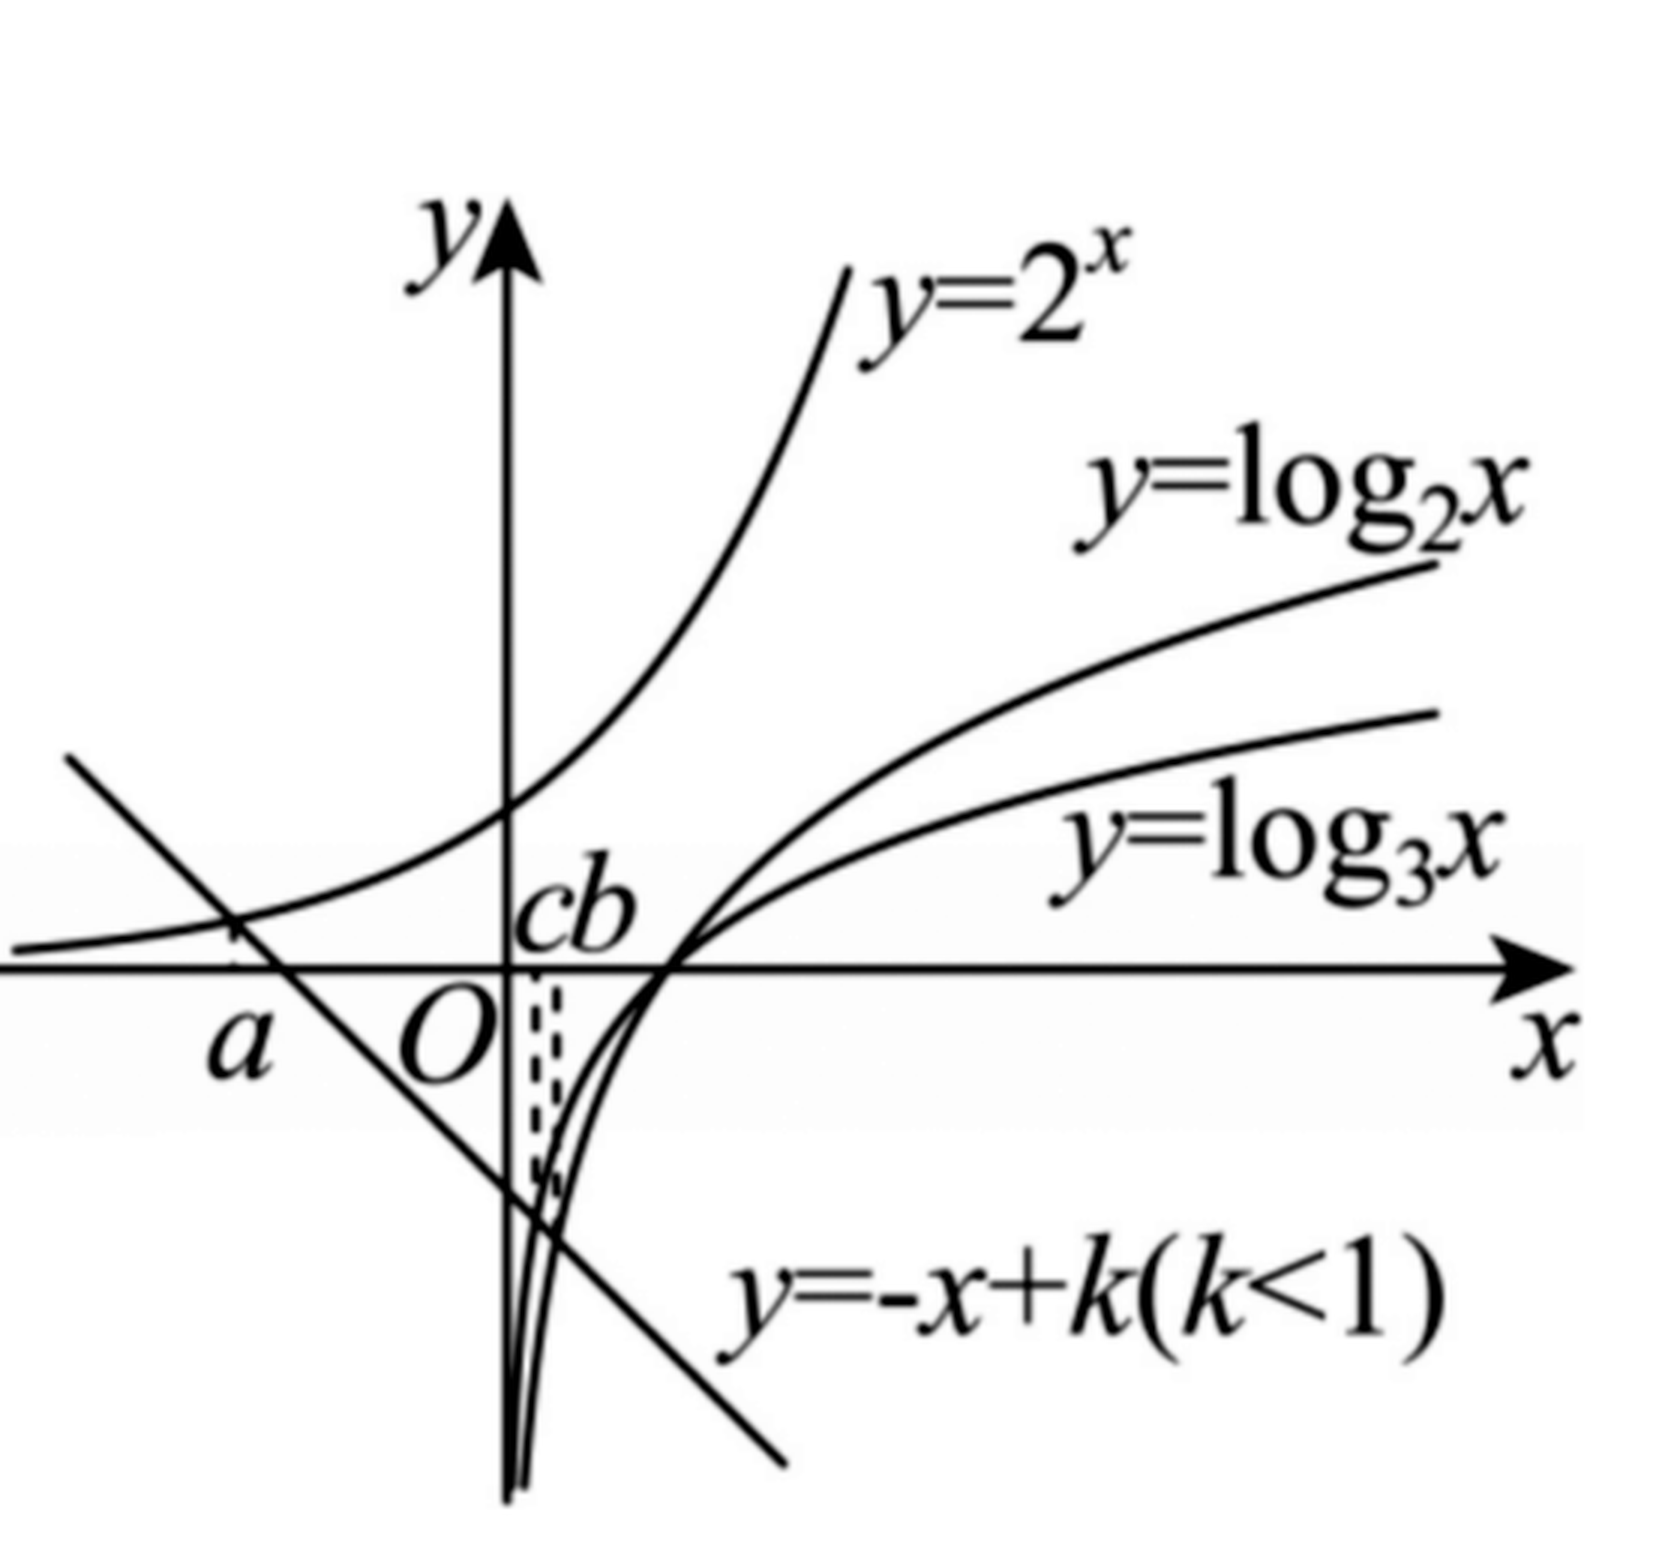
\includegraphics[width=0.52\textwidth]{figures/gao156_q15_curves.png}
\end{center}

\step{如图所示，由图象得 $a<c<b$. 故选 $B$.}
\solend
\fi

% === Q16 === ①② 文本圈数字、"一阶/二阶不动点""稳定点"自定义名词；解析 5 行，故选 A
\item 对定义域为 $I$ 的函数 $y=f(x)$，若存在 $x_0\in I$ 使得 $f(x_0)=x_0$，则称 $x_0$ 是函数 $f(x)$ 的
一阶不动点，简称不动点；若存在 $x_0\in I$ 使得 $f(f(x_0))=x_0$，则称 $x_0$ 是函数 $f(x)$ 的二阶
不动点，简称稳定点. 现有如下两个命题：①存在函数非 $y=x$ 且有无穷多个不动点；②
存在函数有无穷多个稳定点，且这些稳定点不都是不动点. 则\mbox{（\quad）}

\keepwithprev
A. ①成立，②成立\qquad\qquad B. ①成立，②不成立

C. ①不成立，②成立\qquad\qquad D. ①不成立，②不成立

\ifanswer
\solbegin
\step{①取定义在全体实数上的 $f(x)=\lvert x\rvert$，其不动点为一切非负实数，有无穷多个，}
\step{且 $f(-1)=1\ne-1$，①成立.}
\step{②取定义在全体实数上的 $g(x)=-x$，则 $g(g(x))=-(-x)=x$，}
\step{全体实数都是稳定点，而不动点只有 0，②成立.}
\step{故选 $A$.}
\solend
\fi

\end{enumerate}

\bigsec{三、解答题}

\begin{enumerate}
\setcounter{enumi}{16}

% === Q17 === $A\cap B$、$B\cap C$、\varnothing、\mid；解析 6 行
\item 设集合 $A=\{x\mid-1\leqslant x\leqslant2\}$，$B=\{x\mid2m<x<1\}$，$C=\{x\mid x<-1$ 或 $x>2\}$.

(1) 若 $A\cap B=B$，求实数 $m$ 的取值范围；

(2) 若 $B\cap C$ 中只有一个整数，求实数 $m$ 的取值范围.

\ifanswer
\solbegin
\step{(1) 当 $m\geqslant\dfrac12$ 时，$B=\varnothing$，满足 $A\cap B=B$.}
\step{当 $m<\dfrac12$ 时，$A\cap B=B$ 等价于 $2m\geqslant-1$，得 $-\dfrac12\leqslant m<\dfrac12$.}
\step{因此 $m$ 的取值范围为 $\left[-\dfrac12,+\infty\right)$.}
\step{(2) $B\cap C=\{x\mid2m<x<-1\}$，其中只有一个整数时，该整数必为 $-2$.}
\step{包含 $-2$ 且不包含 $-3$，等价于 $-3\leqslant2m<-2$，}
\step{因此 $m$ 的取值范围为 $\left[-\dfrac32,-1\right)$.}
\solend
\fi

% === Q18 === 幂函数 $x^{-\frac13}$、$m\in\R$；解析 12 行，跨 05—06 页
\item 已知幂函数 $f(x)=(3m^2-2m)x^m$（$m\in\R$）在定义域上不单调.

(1) 求函数 $f(x)$ 的解析式；

(2) 若 $f(a+1)<f(-2a+3)$，求实数 $a$ 的取值范围.

\ifanswer
\solbegin
\step{(1) 由幂函数的定义，$3m^2-2m=1$，即 $(3m+1)(m-1)=0$，得 $m=1$ 或 $m=-\dfrac13$.}
\step{当 $m=1$ 时，$f(x)=x$ 在定义域上单调递增，不合题意.}
\step{当 $m=-\dfrac13$ 时，$f(-1)=-1<f(1)=1$，而 $f(1)=1>f(8)=\dfrac12$，}
\step{故 $f(x)$ 在定义域上不单调.}
\step{因此 $f(x)=x^{-\frac13}$，定义域为 $(-\infty,0)\cup(0,+\infty)$.}
\step{(2) 有意义的条件为 $a\ne-1$ 且 $a\ne\dfrac32$.}
\step{当 $a<-1$ 时，$a+1<0<-2a+3$，有 $f(a+1)<0<f(-2a+3)$，}
\step{不等式成立.}
\step{当 $-1<a<\dfrac32$ 时，利用 $f(x)$ 在 $(0,+\infty)$ 上单调递减，}
\step{原不等式等价于 $a+1>-2a+3$，得 $\dfrac23<a<\dfrac32$.}
\step{当 $a>\dfrac32$ 时，$f(a+1)>0>f(-2a+3)$，不等式不成立.}
\step{所以 $a\in(-\infty,-1)\cup\left(\dfrac23,\dfrac32\right)$.}
\solend
\fi

% === Q19 === 两套解法（法一红字 \stepm，法二无标签）；\Delta 与 \subseteq；解析 21 行，跨 06—08 页
\item 已知 $a,c\in\R$，函数 $f(x)=\dfrac{x^2+(3a+1)x+c}{x+a}$.

(1) 若 $a=0$，求函数的定义域，并判断是否存在 $c$ 使得 $y=f(x)$ 图像关于原点对称，说明理由；

(2) 若函数过点 $(1,3)$，且函数 $y=f(x)$ 与 $x$ 轴负半轴有两个不同交点，求此时 $c$ 的值和 $a$ 的取值范围.

\ifanswer
\solbegin
\step{(1) 当 $a=0$ 时，$f(x)=\dfrac{x^2+(3a+1)x+c}{x+a}=\dfrac{x^2+x+c}{x}=x+\dfrac cx+1$，}
\step{故定义域为 $(-\infty,0)\cup(0,+\infty)$；}
\step{若存在实数 $c$，使得函数 $f(x)$ 为奇函数，则必有 $f(x)+f(-x)=0$，}
\step{而 $x+\dfrac cx+1+(-x)+\dfrac c{-x}+1=2\ne0$，}
\step{所以不存在实数 $c$，使得函数 $f(x)$ 为奇函数；}
\step{(2) 函数 $f(x)$ 的图像过点 $(1,3)$，则 $f(1)=\dfrac{1+(3a+1)+c}{1+a}=\dfrac{3a+c+2}{a+1}=3$，}
\step{解得 $c=1$，所以 $f(x)=\dfrac{x^2+(3a+1)x+1}{x+a}$，}
\stepm{法一：}{令 $f(x)=0$，则 $x^2+(3a+1)x+1=0$，此时方程有两不等负根，}
\step{则有 $\begin{cases}\Delta=(3a+1)^2-4>0\\-(3a+1)<0\end{cases}\Rightarrow\begin{cases}a>\dfrac13\text{ 或 }a<-1\\a>-\dfrac13\end{cases}\Rightarrow a>\dfrac13$，}
\step{注意到分母 $x+a\ne0$，则 $x\ne-a$，}
\step{若 $x=-a$ 也是方程 $x^2+(3a+1)x+1=0$ 的解，}
\step{代入方程 $(-a)^2+(3a+1)(-a)+1=0\Rightarrow2a^2+a-1=(a+1)(2a-1)=0$，}
\step{解得 $a=-1$ 或 $a=\dfrac12$，从而 $a\ne\dfrac12$，}
\step{综上，实数 $a$ 的取值范围为 $\left(\dfrac13,\dfrac12\right)\cup\left(\dfrac12,+\infty\right)$.}
\step{令 $g(x)=x^2+(3a+1)x+1$，与 $x$ 轴负半轴有两个交点，}
\step{则 $\begin{cases}-(3a+1)<0\\\Delta=(3a+1)^2-4>0\end{cases}\Rightarrow a>\dfrac13$.}
\step{注意到分母 $x+a\ne0$，则 $x\ne-a$，}
\step{若 $x=-a$ 也是方程 $x^2+(3a+1)x+1=0$ 的解，}
\step{代入方程 $(-a)^2+(3a+1)(-a)+1=0\Rightarrow2a^2+a-1=(a+1)(2a-1)=0$，}
\step{解得 $a=-1$ 或 $a=\dfrac12$，从而 $a\ne\dfrac12$，}
\step{综上，实数 $a$ 的取值范围为 $\left(\dfrac13,\dfrac12\right)\cup\left(\dfrac12,+\infty\right)$.}
\solend
\fi

% === Q20 === $Q$ 常数段 80000 照录；cases 与基本不等式；解析 10 行，跨 08—09 页
\item 某工厂生产某种零件的固定成本为 20000 元，每生产一个零件要增加投入 100 元，已知
总收入 $Q$（单位：元）关于产量 $x$（单位：个）满足函数：$Q=\begin{cases}400x-\dfrac12x^2,&0\leqslant x\leqslant400\\80000,&x>400\end{cases}$.

(1) 将利润 $P$（单位：元）表示为产量 $x$ 的函数；（总收入$=$总成本$+$利润）

(2) 当产量为何值时，零件的单位利润最大？最大单位利润是多少元？（单位利润$=$利润$\div$产量）

\ifanswer
\solbegin
\step{(1) 当 $0\leqslant x\leqslant400$ 时，}
\step{$P(x)=400x-\dfrac12x^2-20000-100x=-\dfrac12x^2+300x-20000$，}
\step{当 $x>400$ 时，$P(x)=80000-100x-20000=60000-100x$，}
\step{故 $P(x)=\begin{cases}-\dfrac12x^2+300x-20000,&0\leqslant x\leqslant400\\60000-100x,&x>400\end{cases}$.}
\step{(2) 设零件的单位利润为 $g(x)$，则 $g(x)=\begin{cases}-\dfrac12x-\dfrac{20000}{x}+300,&0\leqslant x\leqslant400\\\dfrac{60000}{x}-100,&x>400\end{cases}$，}
\step{当 $0\leqslant x\leqslant400$ 时，}
\step{$g(x)=300-\left(\dfrac12x+\dfrac{20000}{x}\right)\leqslant300-2\sqrt{\dfrac x2\cdot\dfrac{20000}{x}}=100$，}
\step{当且仅当 $\dfrac x2=\dfrac{20000}{x}$，即 $x=200$ 时取等号，}
\step{当 $x>400$ 时，$g(x)=\dfrac{60000}{x}-100$，此时无最值，}
\step{故当产量为 200 个，零件的单位利润最大，最大单位利润是 100 元.}
\solend
\fi

% === Q21 === 上升集定义、$D(x_0)=\{d\in\R\mid\cdots\}$、①②③ 文本圈数字、
%            \subseteq 带下划线、$-2^{-x}$；解析 19 行，跨 09—10 页
\item 已知函数 $y=f(x)$ 的定义域为 $\R$. 对任意 $x_0\in\R$，定义集合
$D(x_0)=\{d\in\R\mid f(x_0+d)>f(x_0)\}$，则称 $D(x_0)$ 为函数 $y=f(x)$ 在 $x_0$ 处的上升集.

(1) 若 $f(x)=1-x$，求 $D(-1)$；

(2) 若 $f(x)=\begin{cases}2^x,&x<0\\0,&x=0\\-2^{-x},&x>0\end{cases}$，求 $D(x)$；

(3) 设 $y=f(x)$ 满足：①当 $x<0$ 时，$f(x)=2^x$；②若 $f(x_1)\leqslant f(x_2)$，则
$D(x_2)\subseteq D(x_1)$；③当 $0<x<1$ 时，$f(x)<f(0)$. 证明：$f(0)\geqslant1$.

\ifanswer
\solbegin
\step{(1) $f(-1+d)>f(-1)\Leftrightarrow2-d>2\Leftrightarrow d<0$，所以 $D(-1)=(-\infty,0)$.}
\step{(2) 函数在 $(-\infty,0)$、$(0,+\infty)$ 上分别严格递增，}
\step{且这两个区间上的函数值分别为正、负，$f(0)=0$.}
\step{当 $x<0$ 时，$f(x+d)>f(x)\Leftrightarrow x<x+d<0\Leftrightarrow0<d<-x$，}
\step{当 $x=0$ 时，$f(d)>f(0)\Leftrightarrow d<0$，}
\step{当 $x>0$ 时，$f(x+d)>f(x)\Leftrightarrow x+d\leqslant0$ 或 $x+d>x$}
\step{$\Leftrightarrow d\leqslant-x$ 或 $d>0$，}
\step{因此 $D(x)=\begin{cases}(0,-x),&x<0\\(-\infty,0),&x=0\\(-\infty,-x]\cup(0,+\infty),&x>0\end{cases}$.}
\step{(3) 任取 $a\in(-1,0)$，}
\step{令 $d=-\dfrac a2$，则 $0<d<1$，且 $f(a+d)=2^{\frac a2}>2^a=f(a)$，}
\step{所以 $d\in D(a)$；}
\step{由③，$f(d)<f(0)$，所以 $d\notin D(0)$.}
\step{若 $f(0)\leqslant f(a)$，由②得 $D(a)\subseteq D(0)$，与上述结论矛盾.}
\step{因此，对任意 $a\in(-1,0)$，都有 $f(0)>2^a$.}
\step{特别地 $f(0)>2^{-\frac12}>0$.}
\step{若 $f(0)<1$，取 $a=\dfrac12\log_2 f(0)$，则 $-\dfrac14<a<0$，且}
\step{$2^a=\sqrt{f(0)}>f(0)$，}
\step{与 $f(0)>2^a$ 矛盾.}
\step{所以 $f(0)\geqslant1$.}
\solend
\fi

\end{enumerate}

\end{document}
